\documentclass[12pt]{article}
\usepackage{tikz}
\usetikzlibrary{decorations.pathreplacing}
\usetikzlibrary{positioning}
\usepackage{hyperref}
\usepackage{apacite}
\usepackage{float}
\usepackage{geometry}
\usepackage{setspace}
\usepackage{adjustbox}
\usepackage{multirow}
\usepackage[T1]{fontenc} % for smaller printing smaller than sign correctly in plots
\usepackage[labelfont=bf]{caption} % for captions
\usepackage[toc]{appendix} % toc to show in table of contents
\usepackage{tabularx} % expanding tables
\usepackage{xltabular} % multipage tabularx
\usepackage{amsmath} % Align equations
\usepackage{booktabs} % toprule etc..
\usepackage{parskip}
\usepackage{fontspec}
\usepackage[longnamesfirst]{natbib}
\setstretch{1.5}
\geometry{left=20mm, right=50mm, top=20mm, bottom=10mm, includefoot}
\setmainfont{Times New Roman}
\pagecolor{white}

% Command to remove dot after year in references, see TUM.bst
\makeatletter
\newcommand{\removeperiod}{\@ifnextchar.{\@gobble}\relax}
\makeatother

\interfootnotelinepenalty=10000

\renewcommand{\contentsname}{Table of Contents}

\title{Cross-sectional predictability of stock returns in Nordic stock markets using machine learning methods}
\author{Jesse Keränen}
%add time period to all plot and tables once final

\begin{document}
\begin{titlepage}
\begin{center}
\vspace*{2em}
Master thesis submitted in partial fulfillment of the requirements for the degree\\
Master of Science \\
at Technische Universität München 

\vspace{4em}

\Large\textbf{Cross-sectional predictability of stock returns in Nordic stock markets using machine learning methods}

\vspace{4em}

\end{center}

\begin{tabular}{p{10em} l} 
\multirow[t]{4}{*}{Reviewer} 		& Prof. Dr. Christoph Kaserer\\ 
							& Department of Financial Management and Capital Markets\\ 
							& TUM School of Management\\ 
							& Technische Universität München\\[3ex]
Advisor: 						& Noorhan Elkhayat\\[3ex]
Study program: 				& TUM-BWL\\[3ex]
\multirow[t]{5}{*}{Composed by:} 	& Jesse Keränen\\
							& Motorstraße 64\\
							& 80809 Munich\\
							& Tel.: +49 (0) 1628410926\\
							& Matriculation number: 03748837\\[3ex]
Submitted on: 					& \today \\
\end{tabular}

\thispagestyle{empty}
\end{titlepage}

\newpage
\pagenumbering{Roman}

\tableofcontents

\newpage

\addcontentsline{toc}{section}{List of Figures}
\listoffigures

\newpage

\addcontentsline{toc}{section}{List of Tables}
\listoftables

\newpage

\addcontentsline{toc}{section}{List of Abbreviations}
\section*{List of Abbreviations}
\begin{table}[H] 
\setlength\extrarowheight{10pt}
\newcolumntype{Y}{>{\raggedright\arraybackslash}X}
\begin{tabularx}{\textwidth}{@{\extracolsep{4pt}} l Y l Y} 
EXC.RET & Excess return & SMB & Size factor\\ 
CA & Cash-to-asset ratio & RMRF & Market factor\\
CTO & Capital turnover & HML & Value factor\\
INV & Investment & CMA & Investment factor\\
BEME & Book-to-market ratio & RMW & Profitability factor\\
CFP & Cashflow-to-price ratio & MOM & Momentum factor\\
DEBT & Leverage & VO & Trading volume\\
SP & Sales-to-price ratio & NOSH & Number of shares outstanding\\
EP & Earnings-to-price ratio & L.OBV & One month lagged on-balance volume \\
ROA & Return on assets & L.SD & One month lagged turnover \\
ROE & Return on equity & L.LOG.MV & One month lagged log market value\\
Q & Tobin's Q & L.IDVOL & One month lagged idiosyncratic volatility \\
MOM$_7$ & Intermediate momentum & L.BETA & One month lagged beta\\
MOM$_{12}$ & Momentum & &\\
MOM$_{36}$ & Long-term reversals & &\\
MOM$_{2}$ & Short-term reversals & &\\
MOM.IND & Industry momentum & &\\
L.SD & One month lagged standard deviation & &\\
L.HIGH52 & One month lagged 52 week high price ratio & &\\
\end{tabularx}
\end{table} 

\newpage

\addcontentsline{toc}{section}{List of Symbols}
\section*{List of Symbols}
\begin{tabular}{l l}
$\theta$ & \\
$\hat{r}$ & Predicted return\\
$\overline{r}$ & Mean return\\
$\beta$ & Regression coefficient \\
$\alpha$ & Regression intercept\\
$\epsilon$ & Regression error term\\
$\sigma$ & Standard deviation\\
$w$ & Weight of the security in a portfolio\\
$R^2_{oos}$ & Conservative out-of-sample r squared \\
$R^2_{Trad. \ oos}$ & Traditional out-of-sample r squared \\
\end{tabular}

\newpage

\section{Introduction} \label{Introduction}
\pagenumbering{arabic}
In the year 1808 world was in many ways different compared to what it is today. In 1808 Napoleon was the Emperor of the French Empire and Maximilian I was ruling the Kingdom of Bavaria. In 1808 Finnish war broke out between the Kingdom of Sweden and the Russian Empire which would ultimately lead to the establishment of the autonomous Grand Duchy of Finland. It would still take more than 100 years for Finland to gain its independence. In the same year began the Dano-Swedish war between Sweden and Denmark-Norway. Something historically far less remarkable, but essential for this study happened in 1808 as well. The first stock exchange in a Nordic country was opened in Copenhagen\footnotemark. Slowly after that rest of the Nordic countries would open their own stock exchanges as well. Upon facilitated change of ownership of securities, investors were left with the question how to price these assets. \par

\footnotetext{See: \url{https://www.nasdaqomxnordic.com/about_us?languageId=1&Instrument=SSE101}}

A major breakthrough in this topic happened in the sixties when the capital asset pricing model was first developed \citep{Sharpe1964, Lintner1965}. In the eighties performance of the capital asset pricing model was questioned and scholars started to come up with variables that could explain portions of cross-sectional stock returns that the capital asset pricing model could not. These so-called stock market factors would include variables such as earnings-to-price ratio, leverage and market capitalization \citep{Basu1977, Bhandari1988, BANZ1981}. During these times machine learning gained large interest and artificial neural networks became popular. The next big step in empirical asset pricing happened when Eugene Fama and Kenneth French combined a selection of stock market factors into a coherent three-factor asset pricing model \citep{FAMA19933}. A few years later researchers made breakthroughs to overcome limitations of the generalization of the decision trees, by ensembling multiple randomized trees, which would ultimately lead to the introduction of a machine learning method called random forest \citep{Ho1995, Breiman20015}. \par

Although the three-factor model was a remarkable improvement compared to the capital asset pricing model, it was still not able to explain variation in stock returns completely. Even after the three-factor model lot of new stock market factors have been discovered and in the year 2015, Fama and French extended their three-factor model by two additional factors \citep{FAMA20151}. Characteristic for empirical asset pricing literature in recent years has been a large number of predictive variables. Including more than 100 possibly even strongly correlated explanatory variables, could pose serious challenges to traditional linear regression models. This has led researchers to examine other models that do not suffer from over-parameterization as much as linear regression. In recent years lot of research has applied machine learning methods to capture abnormal returns in stock markets.  \par

%Nordic market introduction
The objective of this study is to apply a set of machine learning methods to well-established asset pricing factors to capture abnormal stock return patterns. This study will focus on four Nordic stock markets namely Denmark, Finland, Norway and Sweden. These four developed markets are relatively homogenous in many aspects. They are geographically close, politically stable and economically interconnected. Denmark, Finland and Sweden all belong to the European Union. Additionally, the stock exchanges of all these three countries are operated by Nasdaq, Inc. Therefore, investors could view them as a single market. European market integration is emphasized also by \citet{FAMA2012457}, but this study focuses on possibly even more integrated Nordic markets. Some of the features that are characteristic for Nordic markets make them fertile ground for stock market anomaly studies. As mentioned Nordic countries are geographically closely located in northern Europe and therefore relatively distant from large European and especially American markets.  \par

One stock market phenomenon that could affect Nordic stock markets is the periphery effect \citep{leivo2011}. It refers to investor behaviour where during times of a crisis investors tend to liquidate their investments first from the markets more distant to them. This increases the volatility of periphery markets and can challenge the efficient market theory. Another common feature that Nordic markets share is the high level of foreign ownership. Share of foreign investments in Nordic stock markets can reach more than 50\%\footnotemark. Given the remote location of Nordic stock markets and their high share of foreign ownership, it is likely that Nordic countries could be subject to periphery effect. Which again can result in abnormal return patterns. \par

\footnotetext{\citet{Butt2018} calculate the share of foreign ownership from IMF Coordinated Direct Investment Survey CDIS data. Foreign ownership share of \citeauthor{Butt2018} is 52\% for Denmark, 42\% for Finland, 35\% for Norway and 56\% for Sweden. %check the source
}

This study contributes to the existing literature in several ways. First of all, it applies a machine learning framework from \citet{guetal} to a new market. The machine learning approach has been previously applied to European markets, but as mentioned this study focuses on an even more coherent Nordic submarket \citep{Drobetz, Fieberg}. The objective is to examine if an investor investing only in Nordic markets could benefit from implementing the machine learning framework of \citet{guetal}. The dataset of the study is unique in the sense that a lot of machine learning approach studies have been conducted in wider markets such as European stock markets, whereas previous Nordic stock market anomaly studies have mainly focused on single markets. Pooling the four Nordic markets ensures us a sufficient amount of data to train complex machine learning models, but also allows us to focus on homogenous clearly defined submarket. \par

Additionally, existing stock market anomaly literature focusing solely on Nordic markets is rather limited. Section \ref{NordicStockMarketAnomalies} introduces the existing Nordic stock market anomaly literature. Characteristic for studies in this section is that they mainly focus on one or two stock market anomalies. As this study constructs 23 stock characteristic anomalies, it allows to us examine anomalies that have not been studied in Nordic stock markets previously. This means that this study cannot only reveal the profitability of the machine learning framework in the Nordic market setting, but it can also reveal evidence of the existence of certain stock market anomalies in Nordic markets. As mentioned lot of Nordic stock market anomaly research focuses only up to two anomalies at a time. Since this study includes 23 anomalies simultaneously, it allows us also to examine the performance of already discovered Nordic anomalies while controlling for many other variables. Applying sophisticated machine learning models allows us to control for more complex interactions. \par

The objective of this study is slightly more ambitious than in existing Nordic stock market anomaly literature. Existing literature mainly examines the existence of anomalies by uni- or multivariate portfolio sorts. Studies predefine variables of interest and form portfolios based on these variables. Then the historical excess returns are investigated. This study goes one step further and attempts to predict stock level out-of-sample returns based on the predefined set of variables. This allows us to evaluate which portion of the return variability these variables are able to capture in addition to the profitability of the strategy. \par

The final contribution of this study is to expand the explanatory variable set. This study includes a variable called on-balance volume. On-balance volume is a technical trading indicator that has not been studied in a great extent as a cross-sectional stock return predictor. Due to the previous strong performance of momentum indicators, this study includes several momentum variables. The extended variable set allows us to examine whether an on-balance anomaly exists in Nordic stock markets or whether including on-balance volume affects the performance of well-established momentum indicators. \par

The structure of this paper goes as follows. In the second chapter introduction to related previous literature is provided. In this chapter performance of different methods and the persistence of different anomalies in different regions are discussed. The third chapter introduces the data used in this study and the filters applied to the data. The fourth chapter presents the methodology. It introduces the implemented models in more detail and describes the measurements applied in order to evaluate the performance of the models. The fifth chapter focuses on benchmarking factors, showing how benchmark factors are constructed and how well they behave in Nordic markets. The sixth chapter describes the results of the empirical study. The chapter is divided to discuss separately predictive accuracy, economic profitability and characteristic importance for the machine learning models. Finally, the last chapter provides a conclusion of the empirical study. \par

\section{Stock return anomaly literature}\label{StockReturnAnomalyLiterature}

Being the largest and most prominent stock market in the world US stock market has been subject to the majority of asset pricing studies. Despite the dominance of US markets in capturing the attraction of academics, a lot of empirical asset pricing literature has been conducted in international settings as well. Characteristic for international asset pricing literature is that instead of focusing on single countries they aggregate stock market data to a certain regional level such as Europe or Asia-Pacific. The following chapter provides an overview of pioneering asset pricing anomaly literature. The focus will mainly be on the literature on the US, European and Nordic markets. US stock markets are chosen because of their significant impact on international stock markets and because most anomalies have been discovered there and therefore majority of the initial studies of these anomalies have been conducted there. European studies provide an interesting perspective for this study since in many of them Nordic countries are included. \par

The chapter introduces the most important anomalies in these markets and how they have been exploited with different methods. This works as a starting point to define a set of factors that will be used in this study. It can be argued that this kind of process when the set of variables is chosen based on their performance in previous studies is one sort of forward-looking information as we try to mimic the information set of a historical investor. On the other hand \citet{JACOBS2020213} only find a reliable post-publication decline in long/short factor returns in the US, which emphasizes the practical potential of this study. \par

\subsection{US stock market anomalies}\label{USStockMarketAnomalies}

Many of the recent cross-sectional stock return studies use the framework of \citet{Lewellen2015} as the base model. He runs 10-year rolling \citet{FamaMacBeth1973} regressions using lagged firm characteristics to predict out-of-sample stock returns. He studies cross sections of US stock returns between 1964 and 2013 using different model settings up to 15 company characteristics. He finds a strong positive correlation between expected returns derived from rolling Fama-MacBeth regressions and realized returns. Additionally, \citeauthor{Lewellen2015} shows that the spread between the realized return of the portfolio formed from stock with the lowest expected returns and the portfolio with the highest expected return is up to 2.36\%. In his study logarithmic market value of equity, logarithmic book-to-market value, momentum and accruals show the strongest statistical power in explaining monthly returns using lagged variables. \par

 \citet{guetal} contribute to the literature by applying machine learning methods to exploit the stock market anomalies. By deploying sophisticated models that do not suffer from over-parameterization as heavily as OLS \citeauthor{guetal} are able to include 94 stock characteristics and their interactions as well as eight aggregated time series variables to their models. \citeauthor{guetal} use a large variety of statistical methods including linear regression, generalized linear models with penalization, dimension reduction via principal components regression and partial least squares, gradient-boosted regression trees, random forest and different settings of neural networks. Out of these gradient-boosted regression trees and neural networks\footnotemark \ explain the monthly out-of-sample stock return the best, reaching out-of-sample $R^{2}$ of 0.33\% and 0.44\% correspondingly whereas the three-factor OLS model introduced by \citet{Lewellen2015} only reaches out-of-sample $R^{2}$ of -3.46\%. \par

\footnotetext{\citet{guetal} use five different settings of neural networks differing by the number of hidden layers. A neural network with three hidden layers reaches the highest $R^{2}_{oos}$ and is reported here.}

Similar to \citet{Lewellen2015}, \citeauthor{guetal} construct portfolios based on the predicted return of different models. Monthly spread in realized return between portfolio constructed from decile of companies with lowest expected return and decile of stocks with highest expected return\footnotemark is 0.94\%, 1.62\% and 2.12\% for models based on OLS, random forest and three-layer neural network correspondingly. \citeauthor{guetal} also show that all methods they examine show somewhat similar patterns on variable importance on return predictability. The most important factors are price trends such as momentum followed by stock liquidity, stock volatility, and valuation ratios. \par
% Deeper neural networks seem to be too complex

\footnotetext{Portfolio returns are average value-weighted returns.}

\subsection{European stock market anomalies}\label{EuropeanStockMarketAnomalies}

As mentioned, the US stock market environment is different in many ways compared to Nordic markets. Fortunately lot of stock market studies have been conducted in Europe. Since Nordic markets are usually just a subset of European markets it can be beneficial to have a look at the European studies. \citet{TOBEK2021100588} study machine learning-based anomaly strategies in an international setting. Their study includes 153 different equity anomalies and they only include anomalies to their data after the documented discovery of corresponding anomalies. This way they can mimic the information set an investor would have had and avoid forward-looking information. \citeauthor{TOBEK2021100588} examine five different models including weighted least squares, penalized weighted least squares, gradient boosting regression trees, random forest and neural networks. Their data set spans from 1990 to 2018. \par

Similar to \citet{guetal} in the US, \citeauthor{TOBEK2021100588} find that strategy using neural networks provides the highest returns on quintile long-short portfolios. The mean return for neural network long-short portfolio in Europe was 0.7\%. Interestingly penalized weighted least square method provided a mean return of 0.65\% which is higher than the return of the random forest-based portfolio's return of 0.40\%. \citeauthor{TOBEK2021100588} find that Industry momentum, lagged momentum, liquidity shocks, 52-week high price, book-to-market value and return on equity are the most important variables for neural networks mode\footnotemark. \par

\footnotetext{\citet{TOBEK2021100588} discover possibilities for training models either only using historical data from the US, using historical data from local markets or using international historical data. Only results for models trained using local data are reported here because that is closest to the setting of this study. Additionally, \citeauthor{TOBEK2021100588} state that the difference between model trained on US data and local data is small.}

Exploiting stock market anomalies using machine learning methods is also studied by \citet{Drobetz}. Their data set contains all companies listed in at least one of the 19 Eurozone countries in December 2020 and spans from 1990 to 2020\footnotemark. \citeauthor{Drobetz} examine the performance of ordinary least squares, penalized least squares, principal component regressions, partial least squares, random forests, gradient boosted regression trees and neural networks on predicting monthly stock level returns exploiting a set of 22 predictions, their two-way interactions and second- and third-order polynomials. Findings of \citeauthor{Drobetz} are similar to \citet{guetal}. They show that with a large number of explanatory variables simple linear regression is not able to explain well out-of-sample stock returns. \par

\footnotetext{Finland is the only country included in the study of \citet{Drobetz} that is also included in this study since it is the only country belonging to the Eurozone.}

Findings of \citet{Drobetz} are also similar to \citet{TOBEK2021100588} in the sense that least squares methods where dimensionality is restricted can actually perform better than tree-based methods. Like in the majority of other literature, \citeauthor{Drobetz} find out that neural networks provide a superior framework for stock return prediction models measured in both explanatory power and economic profitability. The neural network method reaches an out-of-sample $R^{2}$ value of 1.23\% and the long-short portfolio formed based on expected returns derived from the neural networks model provides an average value weighted monthly return of 1.94\%. Similar to \citet{guetal}, \citeauthor{Drobetz} find that the same variables show the most importance across the different models, most notably earnings-to-price ratio and 12-month momentum. \par
%Deeper neural networks seem to be too complex

\citet*{Fieberg} study stock market anomalies in 16 European stock markets using machine learning methods over almost the same period as \citet{Drobetz}\footnotemark. Nevertheless, they choose a slightly different approach where instead of including a vast set of anomalies they only consider six prominent equity factors. Factors \citeauthor{Fieberg} consider are beta, market capitalization, the book-to-market-equity ratio, momentum, investment and operating profitability. These factors correspond to the benchmark factor set of this study discussed in Section \ref{BenchmarkFactors}. Their conclusion endorses the findings of \citet{Drobetz} and \citet{TOBEK2021100588} as they show that more complex machine learning models beat the linear approach in terms of both economic and statistical performance. \par

\footnotetext{Dataset of \citet{Fieberg} contains Denmark, Finland, Norway and Sweden.}

\subsection{Nordic stock market anomalies}\label{NordicStockMarketAnomalies}

This chapter provides an overview of discovered stock market anomalies in different Nordic stock markets. Many studies in this chapter have slightly different objectives than this study. Studies show the existence of the anomalies by constructing a portfolio heavily weighted on a certain factor. Nevertheless, they do not describe the magnitude of the relationship between the factor and the expected stock return. This study has a slightly more ambitious objective and tries to derive return expectations from predefined stock market factors. This literature review serves as a starting point for choosing the most promising stock market factors that have already been studied. \par
%small amount of stocks

The magnitude of value and momentum anomalies in Nordic stock markets are examined in the paper by \citet{grobys}. They combine information from companies listed in the main lists of Danish, Finnish, Norwegian and Swedish stock exchanges between 1991 and 2017. \citeauthor{grobys} measure value with book-to-market value and momentum with past 12-month total shareholder return. \citeauthor{grobys} show that the momentum effect exists in Nordics markets and profitability of momentum strategy is not related to the size factor. Value factor yields also significant excess return, but according to \citeauthor{grobys} it could be partly driven by the size factor, since value premium reduces when accounted for the size. Among all stocks, the monthly average equally weighted long-short return is 1.72\% and 1.25\% for momentum and value strategies correspondingly. Both of the excess returns are statistically highly significant. \citeauthor{grobys} also test combination strategies using signals from both momentum and strategy which yield even stronger results. \par

Value premium has shown consistency in Finnish stock markets. \citet*{Davydov2017MagicFV} examine the profitability of different value investing strategies between 1991 and 2013. \citet{Davydov2017MagicFV} investigate a set of value indicators which included earnings-to-price, book-to-price, cashflow-to-price, dividends-to-price and earnings before income and taxes-to-enterprise value ratios. Additionally, they test the performance of investing strategy where portfolios are formed based on the combined ranking of the company's return on invested capital and earnings before income and taxes-to-enterprise value ratio. \citet{Davydov2017MagicFV} show that returns of all of the value portfolios not only beat the market return but can also not be explained by the four-factor model of \citet{Carhart1997}.  \par
%(Finnish Stock Exchange in the period 1991–2013. In total, the number of companies varies from 39 to 136)
%check the second article from patari and leivo

Similar to \citet{grobys}, \citet{leivo2011} combine value anomaly with momentum anomaly in the Finnish stock market for data set between 1993 and 2008. They show that a two-step portfolio sort that first allocates stocks to three portfolios based on their value indicators and subsequently based on the momentum indicator can capture extraordinary stock returns.\citeauthor{leivo2011} show that including momentum further increases returns of already recognized value sorting. The strategy performs even better when authors allow for a long position in a high value high momentum portfolio and a short position in a low value low momentum portfolio. Excess returns resulting from the two-fold portfolio construction cannot be explained by the capital asset pricing model or two-factor model including also the size factor. It is not a surprise that value and momentum premiums exist in Nordic markets. Value and momentum anomalies are among the most well-documented factors showing persistence in multiple cross-sectional studies \citep[e.g.][]{guetal, Lewellen2015, Drobetz, TOBEK2021100588}. \par
% Helsinki Stock Exchange (HEX; later OMX Helsinki) during the period 1993–2008. E/P, EBITDA/EV, CF/P, dividend yield (D/P), B/P and S/P and combinations.
%re-phrase the text

Nordic stock markets have several characteristic features. One is that all Nordic stock markets are considered to be developed, but also small. Especially market capitalization of companies listed in Nordic stock exchanges are on average much smaller than theri international counterparties. Therefore, it is reasonable to ask whether the liquidity of the stock could be a driving factor of the stock returns. The impact of illiquidity risk on stock returns in the Nordic market setting has been studied by \citet{Butt2018}. \citeauthor{Butt2018} test a variety of different illiquidity measures and find that dollar zero returns is the most profitable illiquidity anomaly measure across all four Nordic markets. Dollar zero return measurement is calculated by dividing the number of days stocks return in US dollars is zero by the total number of trading days. \citeauthor{Butt2018} construct five quintile portfolios based on the liquidity of the stocks with data spanning from 1988 to 2013. They show that in all Nordic markets there exists a large illiquidity premium as the annual difference in equal-weighted return of the most illiquid portfolio and least illiquid portfolio is more than 18\% for Finland, Norway and Sweden. For Denmark premium is slightly smaller 8.8\%. \par

\citet{jokipii2006free} investigate free cash flow anomaly in Finnish stock markets between 1992 and 2002. They construct portfolios from stocks listed in the Finnish stock exchange based on predefined thresholds for free cash flow ratios. These ratios include market value to free cash flow and total debt to free cash flow ratios. A high free cash flow portfolio yields higher returns than the market on average and the excess returns can not be completely explained by weightings in \citet{FAMA19933} risk factors. \par
%Finnish companies during the period 1992-2002. net cash flow from operating activities minus capital expenditures. The net cash flow from operating activities, in turn, is defined as the sum of net income, all non-cash charges and credits (e.g.,  depreciation,  amortization  of  intangibles,  and  deferred  taxes),  extra ordinary items, and net change in working capital

\section{Data}\label{Data}

This section provides an overview of the dataset used in this study. The section starts by introducing overall market characteristics in Nordic stock markets. The section discusses how companies are distributed across Nordic markets and also describes the size properties of the companies in different Nordic markets. This part also describes the static and dynamic screens applied to the Datastream data in order to ensure sufficient data quality. The second part of the section describes the firm-level characteristics considered in this study. This includes stock-level excess returns as well as all independent variables. This part introduces definitions of all variables including which characteristics are included calculation of each variable. Descriptive statistics of the firm-level characteristics are also presented in this part of the study. \par

\subsection{Nordic stock market data}\label{NordicStockMarketData}

The main data source for this study is Refinitv Datastream. Company fundamentals data is collected from Worldscope database. The dataset spans from 1990 January to 2022 December which is shorter than in many previous studies. The reason why the period is limited to 1990 is that the amount of publicly listed companies in Nordic markets was rather low in the 1980s and finding reliable data for the period before 1990 is difficult. The dataset contains all stocks listed in primary markets of corresponding countries including also companies that went bankrupt or were de-listed for any other reason. Therefore, the dataset is not subject to survivorship bias. \par

Table \ref{table:constituteLists} in the appendix shows the constituent lists used in data collection. As highlighted by \citet{Ince2006} data from Datastream can be noisy and uncleaned data could lead to a false statistical inference. Therefore, several static and dynamic screens are applied to the data. Static screens include filtering non-equity securities, securities that are not listed in the respective country and securities that are quoted in a currency other than respective country's currency. Panel A from Table \ref{table:StaticScreens} shows which values are accepted for the type of instrument, ISIN code, code indicating the country of origin of the company, country where the security is listed, currency in which the security is noted and ISIN country code. \par

In order to filter non-common and duplicate stock affiliations keywords indicating such securities are searched from Datastream attributes NAME, ENAME and ECNAME. Panel B of Table \ref{table:StaticScreens} presents the country-specific keywords. These keywords are only searched for securities from specific countries but among all the above-mentioned attributes. Keywords from Table \ref{table:GeneralKeywords} are searched from name attributes of securities from all countries. If a keyword is found from any of the name attributes, the security will be removed from the dataset. Keyword deletion follows \citet{Ince2006} and \citet{HANAUER2023106712}. \par

As mentioned \citet{Ince2006} argue that data quality issues in Datastream could even lead to wrong conclusions. In order to avoid results being driven by extraordinary data points, which could be caused by data quality issues, dynamic screens are applied to the data. Table \ref{table:DynamicScreens} in the appendix presents the applied dynamic screens. Observations are removed from the dataset in case of extreme abnormal returns. Observations are also removed in case of extremely strong strong return reversals.\par

One characteristic has to be taken into consideration when working with data from Datastream. In case the company is delisted for some reason Datastream returns the last available value for the remaining periods in the query. In order to only include actively traded securities these observations have to be cleaned from the dataset. This could be done with variable TIME from Datastream which shows the date of last equity price data. Nevertheless, \citet{Ince2006} argue that the TIME attribute is not a reliable indicator of the delisting date, but propose to remove consecutive zero returns from the end of the dataset. Removal of zero returns from the end of the dataset could lead to the removal of actual zero returns, but the effect of this is considered to be smaller than the noise caused by the usage of TIME variable. Therefore, all consecutive zero returns at the end of the dataset are removed for all companies. \par

\begin{table}[ht] 
\footnotesize
\caption[Country summary statistics]{\textbf{Country summary statistics \textnormal{- Own source}}\\ Table provides summary statistics for pooled Nordic market and separate country-specific Nordic markets. The minimum number of companies tells the number of companies included in the data set in a month that the value was lowest for the respective country. The maximum number of companies tells the number of companies included in the data set in a month that the value was highest for the respective country. The mean number of companies is the time series average of the monthly number of companies for each country. Total number of companies is the number of unique companies in the whole data set. Time series averages for monthly mean, median and total market values are also presented. Total market value is the sum of the market values of the respective country in each month. All marked values are converted to USD. Only companies in the final dataset are included in the calculation of the figures. The micro-cap stocks are excluded from the dataset. The dataset spans from January 1990 to December 2022.}
 \label{table:CountrySummary}
\centering
\newcolumntype{Y}{>{\centering\arraybackslash}X}
\begin{tabularx}{\textwidth}{@{\extracolsep{4pt}} X Y Y Y Y Y Y Y} 
\toprule
 & \multicolumn{4}{c}{Number of companies} & \multicolumn{3}{c}{Market value} \\
\cmidrule{2-5} \cmidrule{6-8} 
Market		& Min 	& Max 	& Mean  	& Total	& Mean 		& Median 	& Total \\
\midrule
Denmark	 	& 42		& 106 	& 70	 	& 235	& 2399.78 	& 810.32	& 141657.9  \\
Finland	 	& 26 		& 83	 	& 62		& 186 	& 1893.43 	& 634.47	& 124389.2 \\
Norway		& 44 		& 132 	& 79	 	& 408	& 1520.75	 	& 506.17  & 124689.5 \\
Sweden		& 45 		& 256 	& 132 	& 593	& 2115.65	 	& 616.59	& 308952.1  \\
\midrule
Nordic		& 200 	& 527 	& 343 	& 1422	& 1946.46 	& 583.02	& 699688.8  \\
\bottomrule
\end{tabularx}
\end{table} 

On average number of companies with large market capitalization is more limited in Nordic countries than in the United States or Europe. The smallest companies can be numerous, but still only account for a fraction of total market capitalization. The liquidity of these companies is often also quite low. To avoid results being driven by such stocks, the approach of \citet{HANAUER2023} for emerging markets is applied and companies with the smallest market value that account for 3\% of the aggregated market value are excluded. On the other hand, we do not want a few extremely large companies to drive the results either. Therefore, the market value of the companies is winsorized monthly to 99\%. If company's market value is among the 1\% biggest market values in the corresponding month, the market value will be replaced by the 1\% threshold value. \par

Table \ref{table:CountrySummary} presents the number of companies and their sizes in separate and pooled Nordic markets after applying the above-described filters. The total number of non-micro cap stocks in the dataset is 1422 whereas the monthly number of stocks in the dataset is 343 on average. Figure \ref{plot:number_of_companies_wo_micro} shows the development of the non-micro-cap company count that passed the static and dynamic screens over time. Figure \ref{plot:number_of_companies} in the appendix shows the development of company counts over time including micro-cap stocks. Comparing the two figures it can be seen that even though micro-cap stocks account only for 3\% of the aggregated market value, they account for a remarkable share of company count also in Nordic stock markets. The maximum number of companies including micro-cap stocks exceeds 1000 whereas the maximum number of companies excluding micro-cap stocks is slightly above 500. \par

Sweden is clearly the biggest of the four Nordic markets both in regards to the number of companies and total market value of the companies. Even though Sweden is the biggest market it is not dominating. On average Sweden accounts for less than half of the total market value of the pooled Nordic market. In regards to average and median market value, Denmark has the biggest companies. Finland on the other hand is clearly the smallest of the markets included in the study measured both in number of companies and market value of the companies. \par

\begin{figure}[ht]
\centering
\caption[Number of non-micro-cap companies]{\textbf{Number of non-micro-cap companies \textnormal{- Own source}}\\ Figure shows the development of the total number of securities considered in the dataset from January 1990 to December 2022 for each Nordic country. The figure counts all non-micro-cap securities that passed the static and dynamic screens.}
% Created by tikzDevice version 0.12.6 on 2024-03-10 22:08:15
% !TEX encoding = UTF-8 Unicode
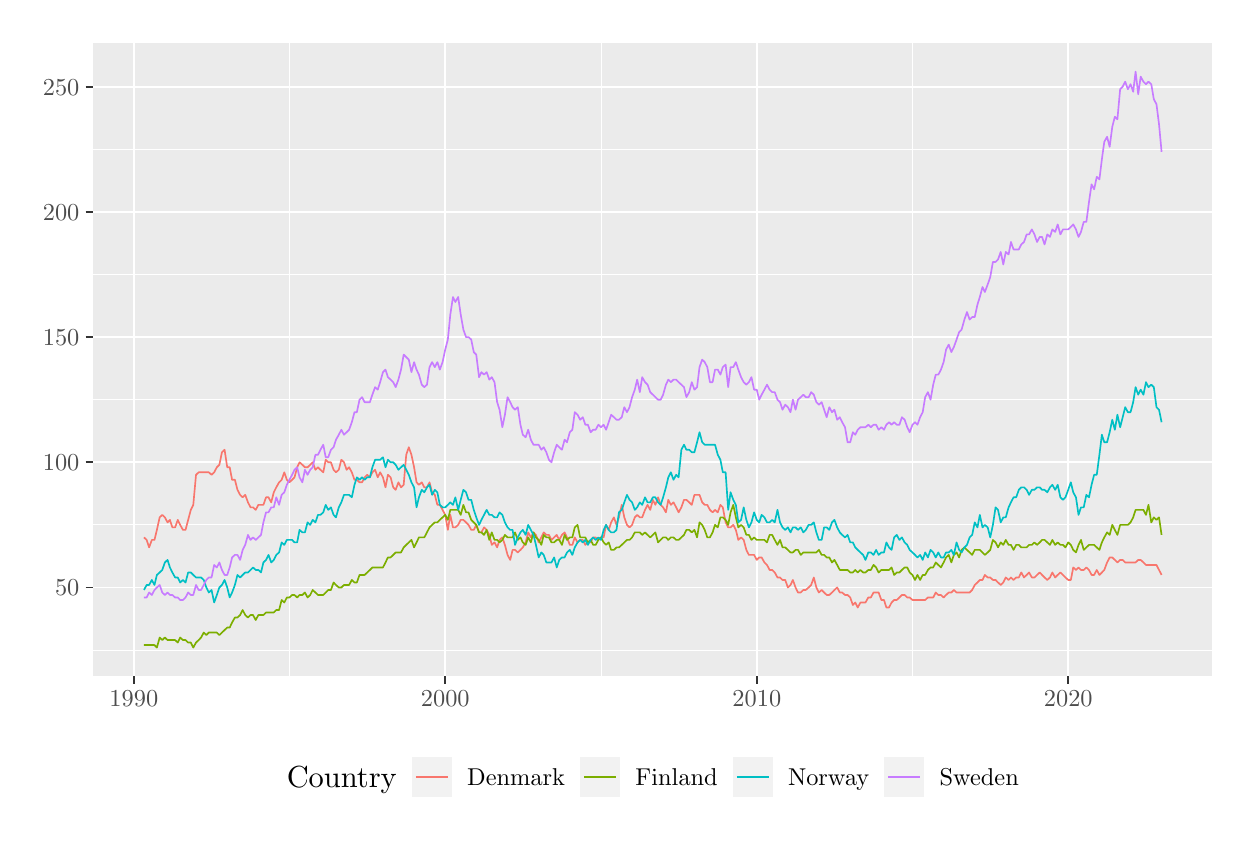
\begin{tikzpicture}[x=1pt,y=1pt]
\definecolor{fillColor}{RGB}{255,255,255}
\path[use as bounding box,fill=fillColor,fill opacity=0.00] (0,0) rectangle (433.62,289.08);
\begin{scope}
\path[clip] (  0.00,  0.00) rectangle (433.62,289.08);
\definecolor{drawColor}{RGB}{255,255,255}
\definecolor{fillColor}{RGB}{255,255,255}

\path[draw=drawColor,line width= 0.6pt,line join=round,line cap=round,fill=fillColor] (  0.00,  0.00) rectangle (433.62,289.08);
\end{scope}
\begin{scope}
\path[clip] ( 23.65, 54.68) rectangle (428.12,283.58);
\definecolor{fillColor}{gray}{0.92}

\path[fill=fillColor] ( 23.65, 54.68) rectangle (428.12,283.58);
\definecolor{drawColor}{RGB}{255,255,255}

\path[draw=drawColor,line width= 0.3pt,line join=round] ( 23.65, 64.18) --
	(428.12, 64.18);

\path[draw=drawColor,line width= 0.3pt,line join=round] ( 23.65,109.41) --
	(428.12,109.41);

\path[draw=drawColor,line width= 0.3pt,line join=round] ( 23.65,154.65) --
	(428.12,154.65);

\path[draw=drawColor,line width= 0.3pt,line join=round] ( 23.65,199.89) --
	(428.12,199.89);

\path[draw=drawColor,line width= 0.3pt,line join=round] ( 23.65,245.13) --
	(428.12,245.13);

\path[draw=drawColor,line width= 0.3pt,line join=round] ( 94.64, 54.68) --
	( 94.64,283.58);

\path[draw=drawColor,line width= 0.3pt,line join=round] (207.19, 54.68) --
	(207.19,283.58);

\path[draw=drawColor,line width= 0.3pt,line join=round] (319.75, 54.68) --
	(319.75,283.58);

\path[draw=drawColor,line width= 0.6pt,line join=round] ( 23.65, 86.79) --
	(428.12, 86.79);

\path[draw=drawColor,line width= 0.6pt,line join=round] ( 23.65,132.03) --
	(428.12,132.03);

\path[draw=drawColor,line width= 0.6pt,line join=round] ( 23.65,177.27) --
	(428.12,177.27);

\path[draw=drawColor,line width= 0.6pt,line join=round] ( 23.65,222.51) --
	(428.12,222.51);

\path[draw=drawColor,line width= 0.6pt,line join=round] ( 23.65,267.75) --
	(428.12,267.75);

\path[draw=drawColor,line width= 0.6pt,line join=round] ( 38.36, 54.68) --
	( 38.36,283.58);

\path[draw=drawColor,line width= 0.6pt,line join=round] (150.91, 54.68) --
	(150.91,283.58);

\path[draw=drawColor,line width= 0.6pt,line join=round] (263.48, 54.68) --
	(263.48,283.58);

\path[draw=drawColor,line width= 0.6pt,line join=round] (376.02, 54.68) --
	(376.02,283.58);
\definecolor{drawColor}{RGB}{248,118,109}

\path[draw=drawColor,line width= 0.6pt,line join=round] ( 42.03,104.89) --
	( 42.99,103.98) --
	( 43.88,101.27) --
	( 44.87,103.98) --
	( 45.82,103.98) --
	( 46.69,107.60) --
	( 47.70,112.13) --
	( 48.63,113.03) --
	( 49.58,112.13) --
	( 50.54,110.32) --
	( 51.40,111.22) --
	( 52.29,108.51) --
	( 53.28,108.51) --
	( 54.24,111.22) --
	( 55.10,109.41) --
	( 56.12,107.60) --
	( 57.04,107.60) --
	( 57.99,111.22) --
	( 58.95,114.84) --
	( 59.84,116.65) --
	( 60.83,127.51) --
	( 61.79,128.41) --
	( 62.65,128.41) --
	( 63.63,128.41) --
	( 64.56,128.41) --
	( 65.45,128.41) --
	( 66.44,127.51) --
	( 67.39,128.41) --
	( 68.35,130.22) --
	( 69.27,131.13) --
	( 70.20,135.65) --
	( 71.15,136.56) --
	( 72.11,130.22) --
	( 73.00,130.22) --
	( 73.87,125.70) --
	( 74.88,125.70) --
	( 75.81,122.08) --
	( 76.76,120.27) --
	( 77.69,119.37) --
	( 78.61,120.27) --
	( 79.60,117.56) --
	( 80.52,115.75) --
	( 81.42,115.75) --
	( 82.40,114.84) --
	( 83.36,116.65) --
	( 84.31,116.65) --
	( 85.18,116.65) --
	( 86.13,119.37) --
	( 87.02,119.37) --
	( 88.01,117.56) --
	( 88.93,121.18) --
	( 89.83,122.98) --
	( 90.85,124.79) --
	( 91.77,125.70) --
	( 92.73,128.41) --
	( 93.65,125.70) --
	( 94.57,124.79) --
	( 95.56,125.70) --
	( 96.42,126.60) --
	( 97.38,130.22) --
	( 98.24,132.03) --
	( 99.26,131.13) --
	(100.18,130.22) --
	(101.14,130.22) --
	(102.09,131.13) --
	(102.99,132.03) --
	(103.97,129.32) --
	(104.90,130.22) --
	(105.79,129.32) --
	(106.81,128.41) --
	(107.70,132.94) --
	(108.60,132.03) --
	(109.58,132.03) --
	(110.54,129.32) --
	(111.40,128.41) --
	(112.42,129.32) --
	(113.34,132.94) --
	(114.30,132.03) --
	(115.25,129.32) --
	(116.15,130.22) --
	(117.13,128.41) --
	(118.09,125.70) --
	(118.95,125.70) --
	(119.91,124.79) --
	(120.83,124.79) --
	(121.75,126.60) --
	(122.71,127.51) --
	(123.66,126.60) --
	(124.56,128.41) --
	(125.54,129.32) --
	(126.50,126.60) --
	(127.36,128.41) --
	(128.38,126.60) --
	(129.30,122.98) --
	(130.17,127.51) --
	(131.15,126.60) --
	(132.08,122.98) --
	(132.97,122.08) --
	(133.96,124.79) --
	(134.91,122.98) --
	(135.87,123.89) --
	(136.79,134.75) --
	(137.72,137.46) --
	(138.67,134.75) --
	(139.63,130.22) --
	(140.52,124.79) --
	(141.38,123.89) --
	(142.40,124.79) --
	(143.33,122.98) --
	(144.28,122.98) --
	(145.21,124.79) --
	(146.13,121.18) --
	(147.12,120.27) --
	(148.04,116.65) --
	(148.93,116.65) --
	(149.92,114.84) --
	(150.88,113.03) --
	(151.83,107.60) --
	(152.72,113.03) --
	(153.68,108.51) --
	(154.54,108.51) --
	(155.56,109.41) --
	(156.48,111.22) --
	(157.44,111.22) --
	(158.40,110.32) --
	(159.29,109.41) --
	(160.28,107.60) --
	(161.20,107.60) --
	(162.09,109.41) --
	(163.11,106.70) --
	(163.97,106.70) --
	(164.90,108.51) --
	(165.85,107.60) --
	(166.81,105.79) --
	(167.70,102.18) --
	(168.69,103.08) --
	(169.64,101.27) --
	(170.51,103.98) --
	(171.52,104.89) --
	(172.45,102.18) --
	(173.40, 98.56) --
	(174.36, 96.75) --
	(175.22,100.37) --
	(176.11,100.37) --
	(177.10, 99.46) --
	(178.06,100.37) --
	(178.92,101.27) --
	(179.94,103.08) --
	(180.86,106.70) --
	(181.82,104.89) --
	(182.77,106.70) --
	(183.66,105.79) --
	(184.65,103.08) --
	(185.61,104.89) --
	(186.47,106.70) --
	(187.42,105.79) --
	(188.35,105.79) --
	(189.27,103.98) --
	(190.23,104.89) --
	(191.18,105.79) --
	(192.08,103.98) --
	(193.06,105.79) --
	(194.02,106.70) --
	(194.88,104.89) --
	(195.90,102.18) --
	(196.82,102.18) --
	(197.69,104.89) --
	(198.70,103.08) --
	(199.63,103.98) --
	(200.58,103.98) --
	(201.51,102.18) --
	(202.43,103.08) --
	(203.42,103.08) --
	(204.34,104.89) --
	(205.24,104.89) --
	(206.22,103.98) --
	(207.18,104.89) --
	(208.13,104.89) --
	(209.00,109.41) --
	(209.95,107.60) --
	(210.84,110.32) --
	(211.83,112.13) --
	(212.76,109.41) --
	(213.65,112.13) --
	(214.67,116.65) --
	(215.59,112.13) --
	(216.55,109.41) --
	(217.47,108.51) --
	(218.40,109.41) --
	(219.38,112.13) --
	(220.24,113.03) --
	(221.20,112.13) --
	(222.06,112.13) --
	(223.08,114.84) --
	(224.00,116.65) --
	(224.96,114.84) --
	(225.91,118.46) --
	(226.81,116.65) --
	(227.79,119.37) --
	(228.72,116.65) --
	(229.61,115.75) --
	(230.63,113.94) --
	(231.49,118.46) --
	(232.42,116.65) --
	(233.37,117.56) --
	(234.33,115.75) --
	(235.22,113.94) --
	(236.21,115.75) --
	(237.16,118.46) --
	(238.03,118.46) --
	(239.04,117.56) --
	(239.97,116.65) --
	(240.92,120.27) --
	(241.88,120.27) --
	(242.77,120.27) --
	(243.73,117.56) --
	(244.65,116.65) --
	(245.58,116.65) --
	(246.53,114.84) --
	(247.49,113.94) --
	(248.38,114.84) --
	(249.37,113.94) --
	(250.32,116.65) --
	(251.18,115.75) --
	(252.20,110.32) --
	(253.13,108.51) --
	(253.99,108.51) --
	(254.97,109.41) --
	(255.90,107.60) --
	(256.79,103.98) --
	(257.78,104.89) --
	(258.73,103.98) --
	(259.69,100.37) --
	(260.61, 98.56) --
	(261.54, 98.56) --
	(262.49, 98.56) --
	(263.45, 96.75) --
	(264.34, 97.65) --
	(265.21, 97.65) --
	(266.22, 95.84) --
	(267.15, 94.94) --
	(268.10, 93.13) --
	(269.03, 93.13) --
	(269.95, 92.22) --
	(270.94, 90.41) --
	(271.86, 90.41) --
	(272.76, 89.51) --
	(273.74, 89.51) --
	(274.70, 86.79) --
	(275.65, 87.70) --
	(276.51, 89.51) --
	(277.47, 86.79) --
	(278.36, 84.98) --
	(279.35, 84.98) --
	(280.27, 85.89) --
	(281.17, 85.89) --
	(282.19, 86.79) --
	(283.11, 87.70) --
	(284.07, 90.41) --
	(284.99, 86.79) --
	(285.91, 84.98) --
	(286.90, 85.89) --
	(287.79, 84.98) --
	(288.72, 84.08) --
	(289.67, 84.08) --
	(290.63, 84.98) --
	(291.52, 85.89) --
	(292.51, 86.79) --
	(293.46, 84.98) --
	(294.33, 84.98) --
	(295.34, 84.08) --
	(296.27, 84.08) --
	(297.22, 83.18) --
	(298.18, 80.46) --
	(299.04, 81.37) --
	(299.94, 79.56) --
	(300.92, 81.37) --
	(301.88, 81.37) --
	(302.74, 81.37) --
	(303.76, 83.18) --
	(304.68, 83.18) --
	(305.64, 84.98) --
	(306.59, 84.98) --
	(307.49, 84.98) --
	(308.47, 82.27) --
	(309.43, 82.27) --
	(310.29, 79.56) --
	(311.25, 79.56) --
	(312.17, 81.37) --
	(313.09, 82.27) --
	(314.05, 82.27) --
	(315.00, 83.18) --
	(315.90, 84.08) --
	(316.88, 84.08) --
	(317.84, 83.18) --
	(318.70, 83.18) --
	(319.72, 82.27) --
	(320.64, 82.27) --
	(321.51, 82.27) --
	(322.49, 82.27) --
	(323.42, 82.27) --
	(324.31, 82.27) --
	(325.30, 83.18) --
	(326.25, 83.18) --
	(327.21, 83.18) --
	(328.13, 84.98) --
	(329.06, 84.08) --
	(330.01, 84.08) --
	(330.97, 83.18) --
	(331.86, 84.08) --
	(332.82, 84.98) --
	(333.77, 84.98) --
	(334.67, 85.89) --
	(335.65, 84.98) --
	(336.58, 84.98) --
	(337.47, 84.98) --
	(338.49, 84.98) --
	(339.41, 84.98) --
	(340.37, 84.98) --
	(341.29, 85.89) --
	(342.22, 87.70) --
	(343.20, 88.60) --
	(344.06, 89.51) --
	(345.02, 89.51) --
	(345.88, 91.32) --
	(346.90, 90.41) --
	(347.82, 90.41) --
	(348.78, 89.51) --
	(349.74, 89.51) --
	(350.63, 88.60) --
	(351.61, 87.70) --
	(352.54, 88.60) --
	(353.43, 90.41) --
	(354.45, 89.51) --
	(355.31, 90.41) --
	(356.24, 89.51) --
	(357.19, 90.41) --
	(358.15, 90.41) --
	(359.04, 92.22) --
	(360.03, 90.41) --
	(360.98, 91.32) --
	(361.85, 92.22) --
	(362.86, 90.41) --
	(363.79, 90.41) --
	(364.74, 91.32) --
	(365.70, 92.22) --
	(366.56, 91.32) --
	(367.45, 90.41) --
	(368.44, 89.51) --
	(369.40, 90.41) --
	(370.26, 92.22) --
	(371.28, 90.41) --
	(372.20, 91.32) --
	(373.16, 92.22) --
	(374.11, 91.32) --
	(375.00, 90.41) --
	(375.99, 89.51) --
	(376.95, 89.51) --
	(377.81, 94.03) --
	(378.80, 93.13) --
	(379.72, 94.03) --
	(380.61, 93.13) --
	(381.60, 93.13) --
	(382.55, 94.03) --
	(383.51, 93.13) --
	(384.43, 91.32) --
	(385.36, 91.32) --
	(386.31, 93.13) --
	(387.27, 91.32) --
	(388.16, 92.22) --
	(389.03, 93.13) --
	(390.04, 95.84) --
	(390.97, 97.65) --
	(391.92, 97.65) --
	(392.85, 96.75) --
	(393.77, 95.84) --
	(394.76, 96.75) --
	(395.68, 96.75) --
	(396.58, 95.84) --
	(397.56, 95.84) --
	(398.52, 95.84) --
	(399.47, 95.84) --
	(400.34, 95.84) --
	(401.29, 96.75) --
	(402.18, 96.75) --
	(403.17, 95.84) --
	(404.10, 94.94) --
	(404.99, 94.94) --
	(406.01, 94.94) --
	(406.93, 94.94) --
	(407.89, 94.94) --
	(408.81, 93.13) --
	(409.73, 91.32);
\definecolor{drawColor}{RGB}{124,174,0}

\path[draw=drawColor,line width= 0.6pt,line join=round] ( 42.03, 65.98) --
	( 42.99, 65.98) --
	( 43.88, 65.98) --
	( 44.87, 65.98) --
	( 45.82, 65.98) --
	( 46.69, 65.08) --
	( 47.70, 68.70) --
	( 48.63, 67.79) --
	( 49.58, 68.70) --
	( 50.54, 67.79) --
	( 51.40, 67.79) --
	( 52.29, 67.79) --
	( 53.28, 67.79) --
	( 54.24, 66.89) --
	( 55.10, 68.70) --
	( 56.12, 67.79) --
	( 57.04, 67.79) --
	( 57.99, 66.89) --
	( 58.95, 66.89) --
	( 59.84, 65.08) --
	( 60.83, 66.89) --
	( 61.79, 67.79) --
	( 62.65, 68.70) --
	( 63.63, 70.51) --
	( 64.56, 69.60) --
	( 65.45, 70.51) --
	( 66.44, 70.51) --
	( 67.39, 70.51) --
	( 68.35, 70.51) --
	( 69.27, 69.60) --
	( 70.20, 70.51) --
	( 71.15, 71.41) --
	( 72.11, 72.32) --
	( 73.00, 72.32) --
	( 73.87, 74.13) --
	( 74.88, 75.94) --
	( 75.81, 75.94) --
	( 76.76, 76.84) --
	( 77.69, 78.65) --
	( 78.61, 76.84) --
	( 79.60, 75.94) --
	( 80.52, 76.84) --
	( 81.42, 76.84) --
	( 82.40, 75.03) --
	( 83.36, 76.84) --
	( 84.31, 76.84) --
	( 85.18, 76.84) --
	( 86.13, 77.75) --
	( 87.02, 77.75) --
	( 88.01, 77.75) --
	( 88.93, 77.75) --
	( 89.83, 78.65) --
	( 90.85, 78.65) --
	( 91.77, 82.27) --
	( 92.73, 81.37) --
	( 93.65, 83.18) --
	( 94.57, 83.18) --
	( 95.56, 84.08) --
	( 96.42, 84.08) --
	( 97.38, 83.18) --
	( 98.24, 84.08) --
	( 99.26, 84.08) --
	(100.18, 84.98) --
	(101.14, 83.18) --
	(102.09, 84.08) --
	(102.99, 85.89) --
	(103.97, 84.98) --
	(104.90, 84.08) --
	(105.79, 84.08) --
	(106.81, 84.08) --
	(107.70, 84.98) --
	(108.60, 85.89) --
	(109.58, 85.89) --
	(110.54, 88.60) --
	(111.40, 87.70) --
	(112.42, 86.79) --
	(113.34, 86.79) --
	(114.30, 87.70) --
	(115.25, 87.70) --
	(116.15, 87.70) --
	(117.13, 89.51) --
	(118.09, 88.60) --
	(118.95, 88.60) --
	(119.91, 91.32) --
	(120.83, 91.32) --
	(121.75, 91.32) --
	(122.71, 92.22) --
	(123.66, 93.13) --
	(124.56, 94.03) --
	(125.54, 94.03) --
	(126.50, 94.03) --
	(127.36, 94.03) --
	(128.38, 94.03) --
	(129.30, 95.84) --
	(130.17, 97.65) --
	(131.15, 97.65) --
	(132.08, 98.56) --
	(132.97, 99.46) --
	(133.96, 99.46) --
	(134.91, 99.46) --
	(135.87,101.27) --
	(136.79,102.18) --
	(137.72,103.08) --
	(138.67,103.98) --
	(139.63,101.27) --
	(140.52,103.08) --
	(141.38,104.89) --
	(142.40,104.89) --
	(143.33,104.89) --
	(144.28,106.70) --
	(145.21,108.51) --
	(146.13,109.41) --
	(147.12,110.32) --
	(148.04,110.32) --
	(148.93,111.22) --
	(149.92,112.13) --
	(150.88,113.03) --
	(151.83,111.22) --
	(152.72,114.84) --
	(153.68,114.84) --
	(154.54,114.84) --
	(155.56,114.84) --
	(156.48,113.03) --
	(157.44,116.65) --
	(158.40,113.94) --
	(159.29,113.94) --
	(160.28,111.22) --
	(161.20,110.32) --
	(162.09,109.41) --
	(163.11,106.70) --
	(163.97,106.70) --
	(164.90,105.79) --
	(165.85,107.60) --
	(166.81,103.98) --
	(167.70,106.70) --
	(168.69,103.98) --
	(169.64,103.98) --
	(170.51,103.08) --
	(171.52,103.98) --
	(172.45,105.79) --
	(173.40,104.89) --
	(174.36,104.89) --
	(175.22,104.89) --
	(176.11,106.70) --
	(177.10,103.98) --
	(178.06,104.89) --
	(178.92,103.08) --
	(179.94,102.18) --
	(180.86,104.89) --
	(181.82,103.08) --
	(182.77,106.70) --
	(183.66,104.89) --
	(184.65,103.98) --
	(185.61,102.18) --
	(186.47,105.79) --
	(187.42,104.89) --
	(188.35,104.89) --
	(189.27,103.08) --
	(190.23,103.08) --
	(191.18,103.98) --
	(192.08,103.98) --
	(193.06,102.18) --
	(194.02,105.79) --
	(194.88,103.98) --
	(195.90,104.89) --
	(196.82,104.89) --
	(197.69,108.51) --
	(198.70,109.41) --
	(199.63,104.89) --
	(200.58,104.89) --
	(201.51,104.89) --
	(202.43,103.08) --
	(203.42,103.98) --
	(204.34,102.18) --
	(205.24,102.18) --
	(206.22,103.98) --
	(207.18,104.89) --
	(208.13,103.08) --
	(209.00,102.18) --
	(209.95,103.08) --
	(210.84,100.37) --
	(211.83,100.37) --
	(212.76,101.27) --
	(213.65,101.27) --
	(214.67,102.18) --
	(215.59,103.08) --
	(216.55,103.98) --
	(217.47,103.98) --
	(218.40,104.89) --
	(219.38,106.70) --
	(220.24,106.70) --
	(221.20,106.70) --
	(222.06,105.79) --
	(223.08,106.70) --
	(224.00,105.79) --
	(224.96,104.89) --
	(225.91,105.79) --
	(226.81,106.70) --
	(227.79,103.08) --
	(228.72,103.98) --
	(229.61,104.89) --
	(230.63,104.89) --
	(231.49,103.98) --
	(232.42,104.89) --
	(233.37,104.89) --
	(234.33,103.98) --
	(235.22,103.98) --
	(236.21,104.89) --
	(237.16,105.79) --
	(238.03,107.60) --
	(239.04,107.60) --
	(239.97,106.70) --
	(240.92,107.60) --
	(241.88,104.89) --
	(242.77,110.32) --
	(243.73,109.41) --
	(244.65,107.60) --
	(245.58,104.89) --
	(246.53,104.89) --
	(247.49,106.70) --
	(248.38,109.41) --
	(249.37,108.51) --
	(250.32,112.13) --
	(251.18,112.13) --
	(252.20,111.22) --
	(253.13,109.41) --
	(253.99,113.94) --
	(254.97,116.65) --
	(255.90,112.13) --
	(256.79,108.51) --
	(257.78,109.41) --
	(258.73,108.51) --
	(259.69,105.79) --
	(260.61,105.79) --
	(261.54,103.98) --
	(262.49,104.89) --
	(263.45,103.98) --
	(264.34,103.98) --
	(265.21,103.98) --
	(266.22,103.98) --
	(267.15,103.08) --
	(268.10,105.79) --
	(269.03,105.79) --
	(269.95,103.98) --
	(270.94,102.18) --
	(271.86,103.98) --
	(272.76,101.27) --
	(273.74,101.27) --
	(274.70,100.37) --
	(275.65, 99.46) --
	(276.51, 99.46) --
	(277.47,100.37) --
	(278.36,100.37) --
	(279.35, 98.56) --
	(280.27, 99.46) --
	(281.17, 99.46) --
	(282.19, 99.46) --
	(283.11, 99.46) --
	(284.07, 99.46) --
	(284.99, 99.46) --
	(285.91,100.37) --
	(286.90, 98.56) --
	(287.79, 98.56) --
	(288.72, 97.65) --
	(289.67, 97.65) --
	(290.63, 95.84) --
	(291.52, 96.75) --
	(292.51, 94.94) --
	(293.46, 93.13) --
	(294.33, 93.13) --
	(295.34, 93.13) --
	(296.27, 93.13) --
	(297.22, 92.22) --
	(298.18, 92.22) --
	(299.04, 93.13) --
	(299.94, 92.22) --
	(300.92, 93.13) --
	(301.88, 92.22) --
	(302.74, 92.22) --
	(303.76, 93.13) --
	(304.68, 93.13) --
	(305.64, 94.94) --
	(306.59, 94.03) --
	(307.49, 92.22) --
	(308.47, 93.13) --
	(309.43, 93.13) --
	(310.29, 93.13) --
	(311.25, 93.13) --
	(312.17, 94.03) --
	(313.09, 91.32) --
	(314.05, 92.22) --
	(315.00, 92.22) --
	(315.90, 93.13) --
	(316.88, 94.03) --
	(317.84, 94.03) --
	(318.70, 92.22) --
	(319.72, 91.32) --
	(320.64, 89.51) --
	(321.51, 91.32) --
	(322.49, 89.51) --
	(323.42, 91.32) --
	(324.31, 91.32) --
	(325.30, 93.13) --
	(326.25, 94.03) --
	(327.21, 94.03) --
	(328.13, 95.84) --
	(329.06, 94.94) --
	(330.01, 94.03) --
	(330.97, 95.84) --
	(331.86, 97.65) --
	(332.82, 98.56) --
	(333.77, 95.84) --
	(334.67, 98.56) --
	(335.65, 99.46) --
	(336.58, 97.65) --
	(337.47,100.37) --
	(338.49,101.27) --
	(339.41,100.37) --
	(340.37, 99.46) --
	(341.29, 98.56) --
	(342.22,100.37) --
	(343.20,100.37) --
	(344.06,100.37) --
	(345.02, 99.46) --
	(345.88, 98.56) --
	(346.90, 99.46) --
	(347.82,100.37) --
	(348.78,103.98) --
	(349.74,103.08) --
	(350.63,101.27) --
	(351.61,103.08) --
	(352.54,102.18) --
	(353.43,103.98) --
	(354.45,102.18) --
	(355.31,102.18) --
	(356.24,100.37) --
	(357.19,102.18) --
	(358.15,102.18) --
	(359.04,101.27) --
	(360.03,101.27) --
	(360.98,101.27) --
	(361.85,102.18) --
	(362.86,102.18) --
	(363.79,103.08) --
	(364.74,102.18) --
	(365.70,103.08) --
	(366.56,103.98) --
	(367.45,103.98) --
	(368.44,103.08) --
	(369.40,102.18) --
	(370.26,103.98) --
	(371.28,102.18) --
	(372.20,103.08) --
	(373.16,102.18) --
	(374.11,102.18) --
	(375.00,101.27) --
	(375.99,103.08) --
	(376.95,102.18) --
	(377.81,100.37) --
	(378.80, 99.46) --
	(379.72,102.18) --
	(380.61,103.98) --
	(381.60,100.37) --
	(382.55,101.27) --
	(383.51,102.18) --
	(384.43,102.18) --
	(385.36,102.18) --
	(386.31,101.27) --
	(387.27,100.37) --
	(388.16,103.08) --
	(389.03,104.89) --
	(390.04,106.70) --
	(390.97,105.79) --
	(391.92,109.41) --
	(392.85,107.60) --
	(393.77,105.79) --
	(394.76,109.41) --
	(395.68,109.41) --
	(396.58,109.41) --
	(397.56,109.41) --
	(398.52,110.32) --
	(399.47,112.13) --
	(400.34,114.84) --
	(401.29,114.84) --
	(402.18,114.84) --
	(403.17,114.84) --
	(404.10,113.03) --
	(404.99,116.65) --
	(406.01,110.32) --
	(406.93,112.13) --
	(407.89,111.22) --
	(408.81,112.13) --
	(409.73,105.79);
\definecolor{drawColor}{RGB}{0,191,196}

\path[draw=drawColor,line width= 0.6pt,line join=round] ( 42.03, 85.89) --
	( 42.99, 87.70) --
	( 43.88, 87.70) --
	( 44.87, 89.51) --
	( 45.82, 87.70) --
	( 46.69, 91.32) --
	( 47.70, 92.22) --
	( 48.63, 93.13) --
	( 49.58, 95.84) --
	( 50.54, 96.75) --
	( 51.40, 94.03) --
	( 52.29, 92.22) --
	( 53.28, 90.41) --
	( 54.24, 90.41) --
	( 55.10, 88.60) --
	( 56.12, 89.51) --
	( 57.04, 88.60) --
	( 57.99, 92.22) --
	( 58.95, 92.22) --
	( 59.84, 91.32) --
	( 60.83, 90.41) --
	( 61.79, 90.41) --
	( 62.65, 90.41) --
	( 63.63, 89.51) --
	( 64.56, 86.79) --
	( 65.45, 84.98) --
	( 66.44, 85.89) --
	( 67.39, 81.37) --
	( 68.35, 84.08) --
	( 69.27, 86.79) --
	( 70.20, 87.70) --
	( 71.15, 89.51) --
	( 72.11, 86.79) --
	( 73.00, 83.18) --
	( 73.87, 84.98) --
	( 74.88, 87.70) --
	( 75.81, 91.32) --
	( 76.76, 90.41) --
	( 77.69, 91.32) --
	( 78.61, 92.22) --
	( 79.60, 92.22) --
	( 80.52, 93.13) --
	( 81.42, 94.03) --
	( 82.40, 93.13) --
	( 83.36, 93.13) --
	( 84.31, 92.22) --
	( 85.18, 95.84) --
	( 86.13, 96.75) --
	( 87.02, 98.56) --
	( 88.01, 95.84) --
	( 88.93, 96.75) --
	( 89.83, 98.56) --
	( 90.85, 99.46) --
	( 91.77,103.08) --
	( 92.73,102.18) --
	( 93.65,103.98) --
	( 94.57,103.98) --
	( 95.56,103.98) --
	( 96.42,103.08) --
	( 97.38,103.08) --
	( 98.24,107.60) --
	( 99.26,106.70) --
	(100.18,106.70) --
	(101.14,110.32) --
	(102.09,109.41) --
	(102.99,111.22) --
	(103.97,110.32) --
	(104.90,113.03) --
	(105.79,113.03) --
	(106.81,113.94) --
	(107.70,116.65) --
	(108.60,114.84) --
	(109.58,115.75) --
	(110.54,113.03) --
	(111.40,112.13) --
	(112.42,115.75) --
	(113.34,117.56) --
	(114.30,120.27) --
	(115.25,120.27) --
	(116.15,120.27) --
	(117.13,119.37) --
	(118.09,123.89) --
	(118.95,126.60) --
	(119.91,125.70) --
	(120.83,126.60) --
	(121.75,125.70) --
	(122.71,126.60) --
	(123.66,126.60) --
	(124.56,130.22) --
	(125.54,132.94) --
	(126.50,132.94) --
	(127.36,132.94) --
	(128.38,133.84) --
	(129.30,130.22) --
	(130.17,132.94) --
	(131.15,132.03) --
	(132.08,132.03) --
	(132.97,131.13) --
	(133.96,129.32) --
	(134.91,130.22) --
	(135.87,131.13) --
	(136.79,129.32) --
	(137.72,127.51) --
	(138.67,124.79) --
	(139.63,122.98) --
	(140.52,115.75) --
	(141.38,119.37) --
	(142.40,122.08) --
	(143.33,121.18) --
	(144.28,122.98) --
	(145.21,123.89) --
	(146.13,120.27) --
	(147.12,122.08) --
	(148.04,121.18) --
	(148.93,116.65) --
	(149.92,115.75) --
	(150.88,115.75) --
	(151.83,116.65) --
	(152.72,117.56) --
	(153.68,116.65) --
	(154.54,119.37) --
	(155.56,114.84) --
	(156.48,118.46) --
	(157.44,122.08) --
	(158.40,121.18) --
	(159.29,118.46) --
	(160.28,118.46) --
	(161.20,114.84) --
	(162.09,112.13) --
	(163.11,109.41) --
	(163.97,111.22) --
	(164.90,113.03) --
	(165.85,114.84) --
	(166.81,113.03) --
	(167.70,113.03) --
	(168.69,112.13) --
	(169.64,112.13) --
	(170.51,113.94) --
	(171.52,113.03) --
	(172.45,110.32) --
	(173.40,108.51) --
	(174.36,107.60) --
	(175.22,107.60) --
	(176.11,102.18) --
	(177.10,104.89) --
	(178.06,106.70) --
	(178.92,107.60) --
	(179.94,105.79) --
	(180.86,109.41) --
	(181.82,107.60) --
	(182.77,105.79) --
	(183.66,102.18) --
	(184.65, 97.65) --
	(185.61, 99.46) --
	(186.47, 98.56) --
	(187.42, 95.84) --
	(188.35, 95.84) --
	(189.27, 95.84) --
	(190.23, 97.65) --
	(191.18, 94.03) --
	(192.08, 96.75) --
	(193.06, 97.65) --
	(194.02, 97.65) --
	(194.88, 99.46) --
	(195.90,100.37) --
	(196.82, 98.56) --
	(197.69,101.27) --
	(198.70,103.08) --
	(199.63,103.98) --
	(200.58,103.08) --
	(201.51,103.98) --
	(202.43,102.18) --
	(203.42,103.98) --
	(204.34,104.89) --
	(205.24,103.98) --
	(206.22,104.89) --
	(207.18,103.98) --
	(208.13,107.60) --
	(209.00,109.41) --
	(209.95,107.60) --
	(210.84,106.70) --
	(211.83,106.70) --
	(212.76,107.60) --
	(213.65,113.94) --
	(214.67,114.84) --
	(215.59,117.56) --
	(216.55,120.27) --
	(217.47,118.46) --
	(218.40,117.56) --
	(219.38,114.84) --
	(220.24,115.75) --
	(221.20,117.56) --
	(222.06,116.65) --
	(223.08,119.37) --
	(224.00,117.56) --
	(224.96,117.56) --
	(225.91,119.37) --
	(226.81,119.37) --
	(227.79,117.56) --
	(228.72,116.65) --
	(229.61,119.37) --
	(230.63,122.98) --
	(231.49,126.60) --
	(232.42,128.41) --
	(233.37,125.70) --
	(234.33,127.51) --
	(235.22,126.60) --
	(236.21,136.56) --
	(237.16,138.37) --
	(238.03,136.56) --
	(239.04,136.56) --
	(239.97,135.65) --
	(240.92,135.65) --
	(241.88,139.27) --
	(242.77,142.89) --
	(243.73,139.27) --
	(244.65,138.37) --
	(245.58,138.37) --
	(246.53,138.37) --
	(247.49,138.37) --
	(248.38,138.37) --
	(249.37,134.75) --
	(250.32,132.94) --
	(251.18,128.41) --
	(252.20,128.41) --
	(253.13,114.84) --
	(253.99,121.18) --
	(254.97,118.46) --
	(255.90,116.65) --
	(256.79,110.32) --
	(257.78,111.22) --
	(258.73,115.75) --
	(259.69,111.22) --
	(260.61,108.51) --
	(261.54,110.32) --
	(262.49,113.94) --
	(263.45,111.22) --
	(264.34,110.32) --
	(265.21,113.03) --
	(266.22,112.13) --
	(267.15,110.32) --
	(268.10,110.32) --
	(269.03,111.22) --
	(269.95,110.32) --
	(270.94,114.84) --
	(271.86,110.32) --
	(272.76,108.51) --
	(273.74,107.60) --
	(274.70,108.51) --
	(275.65,106.70) --
	(276.51,108.51) --
	(277.47,108.51) --
	(278.36,107.60) --
	(279.35,108.51) --
	(280.27,106.70) --
	(281.17,107.60) --
	(282.19,109.41) --
	(283.11,109.41) --
	(284.07,110.32) --
	(284.99,106.70) --
	(285.91,103.98) --
	(286.90,103.98) --
	(287.79,108.51) --
	(288.72,108.51) --
	(289.67,107.60) --
	(290.63,110.32) --
	(291.52,111.22) --
	(292.51,108.51) --
	(293.46,106.70) --
	(294.33,105.79) --
	(295.34,104.89) --
	(296.27,105.79) --
	(297.22,103.08) --
	(298.18,103.08) --
	(299.04,101.27) --
	(299.94,100.37) --
	(300.92, 99.46) --
	(301.88, 98.56) --
	(302.74, 96.75) --
	(303.76, 99.46) --
	(304.68, 99.46) --
	(305.64, 98.56) --
	(306.59,100.37) --
	(307.49, 98.56) --
	(308.47, 99.46) --
	(309.43, 99.46) --
	(310.29,103.08) --
	(311.25,101.27) --
	(312.17,100.37) --
	(313.09,104.89) --
	(314.05,105.79) --
	(315.00,103.98) --
	(315.90,104.89) --
	(316.88,103.08) --
	(317.84,102.18) --
	(318.70,100.37) --
	(319.72, 99.46) --
	(320.64, 98.56) --
	(321.51, 97.65) --
	(322.49, 98.56) --
	(323.42, 96.75) --
	(324.31, 99.46) --
	(325.30, 97.65) --
	(326.25,100.37) --
	(327.21, 99.46) --
	(328.13, 97.65) --
	(329.06, 99.46) --
	(330.01, 97.65) --
	(330.97, 97.65) --
	(331.86, 99.46) --
	(332.82, 99.46) --
	(333.77,100.37) --
	(334.67, 98.56) --
	(335.65,103.08) --
	(336.58,100.37) --
	(337.47, 99.46) --
	(338.49,101.27) --
	(339.41,102.18) --
	(340.37,104.89) --
	(341.29,105.79) --
	(342.22,110.32) --
	(343.20,108.51) --
	(344.06,113.03) --
	(345.02,108.51) --
	(345.88,109.41) --
	(346.90,108.51) --
	(347.82,104.89) --
	(348.78,109.41) --
	(349.74,115.75) --
	(350.63,114.84) --
	(351.61,110.32) --
	(352.54,112.13) --
	(353.43,112.13) --
	(354.45,115.75) --
	(355.31,117.56) --
	(356.24,119.37) --
	(357.19,119.37) --
	(358.15,122.08) --
	(359.04,122.98) --
	(360.03,122.98) --
	(360.98,122.08) --
	(361.85,120.27) --
	(362.86,122.08) --
	(363.79,122.08) --
	(364.74,122.98) --
	(365.70,122.98) --
	(366.56,122.08) --
	(367.45,122.08) --
	(368.44,121.18) --
	(369.40,122.98) --
	(370.26,123.89) --
	(371.28,122.08) --
	(372.20,123.89) --
	(373.16,119.37) --
	(374.11,118.46) --
	(375.00,119.37) --
	(375.99,122.08) --
	(376.95,124.79) --
	(377.81,121.18) --
	(378.80,119.37) --
	(379.72,113.03) --
	(380.61,115.75) --
	(381.60,115.75) --
	(382.55,120.27) --
	(383.51,119.37) --
	(384.43,123.89) --
	(385.36,127.51) --
	(386.31,127.51) --
	(387.27,134.75) --
	(388.16,141.98) --
	(389.03,139.27) --
	(390.04,139.27) --
	(390.97,142.89) --
	(391.92,147.41) --
	(392.85,143.79) --
	(393.77,149.22) --
	(394.76,144.70) --
	(395.68,148.32) --
	(396.58,151.94) --
	(397.56,150.13) --
	(398.52,150.13) --
	(399.47,153.75) --
	(400.34,159.18) --
	(401.29,156.46) --
	(402.18,158.27) --
	(403.17,156.46) --
	(404.10,160.98) --
	(404.99,159.18) --
	(406.01,160.08) --
	(406.93,159.18) --
	(407.89,151.94) --
	(408.81,151.03) --
	(409.73,146.51);
\definecolor{drawColor}{RGB}{199,124,255}

\path[draw=drawColor,line width= 0.6pt,line join=round] ( 42.03, 83.18) --
	( 42.99, 83.18) --
	( 43.88, 84.98) --
	( 44.87, 84.08) --
	( 45.82, 85.89) --
	( 46.69, 86.79) --
	( 47.70, 87.70) --
	( 48.63, 84.98) --
	( 49.58, 84.08) --
	( 50.54, 84.98) --
	( 51.40, 84.08) --
	( 52.29, 84.08) --
	( 53.28, 83.18) --
	( 54.24, 83.18) --
	( 55.10, 82.27) --
	( 56.12, 82.27) --
	( 57.04, 83.18) --
	( 57.99, 84.98) --
	( 58.95, 84.08) --
	( 59.84, 84.08) --
	( 60.83, 87.70) --
	( 61.79, 85.89) --
	( 62.65, 85.89) --
	( 63.63, 87.70) --
	( 64.56, 89.51) --
	( 65.45, 90.41) --
	( 66.44, 90.41) --
	( 67.39, 94.94) --
	( 68.35, 94.03) --
	( 69.27, 95.84) --
	( 70.20, 93.13) --
	( 71.15, 91.32) --
	( 72.11, 91.32) --
	( 73.00, 94.03) --
	( 73.87, 97.65) --
	( 74.88, 98.56) --
	( 75.81, 98.56) --
	( 76.76, 96.75) --
	( 77.69,100.37) --
	( 78.61,102.18) --
	( 79.60,105.79) --
	( 80.52,103.98) --
	( 81.42,104.89) --
	( 82.40,103.98) --
	( 83.36,104.89) --
	( 84.31,105.79) --
	( 85.18,110.32) --
	( 86.13,113.94) --
	( 87.02,113.94) --
	( 88.01,115.75) --
	( 88.93,115.75) --
	( 89.83,119.37) --
	( 90.85,116.65) --
	( 91.77,120.27) --
	( 92.73,121.18) --
	( 93.65,123.89) --
	( 94.57,125.70) --
	( 95.56,127.51) --
	( 96.42,129.32) --
	( 97.38,130.22) --
	( 98.24,126.60) --
	( 99.26,124.79) --
	(100.18,129.32) --
	(101.14,127.51) --
	(102.09,129.32) --
	(102.99,130.22) --
	(103.97,134.75) --
	(104.90,134.75) --
	(105.79,136.56) --
	(106.81,138.37) --
	(107.70,133.84) --
	(108.60,133.84) --
	(109.58,136.56) --
	(110.54,137.46) --
	(111.40,140.18) --
	(112.42,141.98) --
	(113.34,143.79) --
	(114.30,141.98) --
	(115.25,142.89) --
	(116.15,143.79) --
	(117.13,146.51) --
	(118.09,150.13) --
	(118.95,150.13) --
	(119.91,154.65) --
	(120.83,155.56) --
	(121.75,153.75) --
	(122.71,153.75) --
	(123.66,153.75) --
	(124.56,156.46) --
	(125.54,159.18) --
	(126.50,158.27) --
	(127.36,160.98) --
	(128.38,164.60) --
	(129.30,165.51) --
	(130.17,162.79) --
	(131.15,161.89) --
	(132.08,160.98) --
	(132.97,159.18) --
	(133.96,161.89) --
	(134.91,165.51) --
	(135.87,170.94) --
	(136.79,170.03) --
	(137.72,169.13) --
	(138.67,164.60) --
	(139.63,168.22) --
	(140.52,165.51) --
	(141.38,163.70) --
	(142.40,160.08) --
	(143.33,159.18) --
	(144.28,160.08) --
	(145.21,166.41) --
	(146.13,168.22) --
	(147.12,166.41) --
	(148.04,168.22) --
	(148.93,165.51) --
	(149.92,168.22) --
	(150.88,172.75) --
	(151.83,176.37) --
	(152.72,185.41) --
	(153.68,191.75) --
	(154.54,189.94) --
	(155.56,191.75) --
	(156.48,185.41) --
	(157.44,179.98) --
	(158.40,177.27) --
	(159.29,177.27) --
	(160.28,176.37) --
	(161.20,171.84) --
	(162.09,170.94) --
	(163.11,162.79) --
	(163.97,164.60) --
	(164.90,163.70) --
	(165.85,164.60) --
	(166.81,161.89) --
	(167.70,162.79) --
	(168.69,160.98) --
	(169.64,153.75) --
	(170.51,151.03) --
	(171.52,144.70) --
	(172.45,149.22) --
	(173.40,155.56) --
	(174.36,153.75) --
	(175.22,151.94) --
	(176.11,151.03) --
	(177.10,151.94) --
	(178.06,145.60) --
	(178.92,141.98) --
	(179.94,141.08) --
	(180.86,143.79) --
	(181.82,140.18) --
	(182.77,138.37) --
	(183.66,138.37) --
	(184.65,138.37) --
	(185.61,136.56) --
	(186.47,137.46) --
	(187.42,135.65) --
	(188.35,132.94) --
	(189.27,132.03) --
	(190.23,135.65) --
	(191.18,138.37) --
	(192.08,137.46) --
	(193.06,136.56) --
	(194.02,140.18) --
	(194.88,139.27) --
	(195.90,142.89) --
	(196.82,143.79) --
	(197.69,150.13) --
	(198.70,149.22) --
	(199.63,147.41) --
	(200.58,148.32) --
	(201.51,145.60) --
	(202.43,145.60) --
	(203.42,142.89) --
	(204.34,143.79) --
	(205.24,143.79) --
	(206.22,145.60) --
	(207.18,144.70) --
	(208.13,145.60) --
	(209.00,143.79) --
	(209.95,146.51) --
	(210.84,149.22) --
	(211.83,148.32) --
	(212.76,147.41) --
	(213.65,147.41) --
	(214.67,148.32) --
	(215.59,151.94) --
	(216.55,150.13) --
	(217.47,151.94) --
	(218.40,155.56) --
	(219.38,158.27) --
	(220.24,161.89) --
	(221.20,157.37) --
	(222.06,162.79) --
	(223.08,160.98) --
	(224.00,160.08) --
	(224.96,157.37) --
	(225.91,156.46) --
	(226.81,155.56) --
	(227.79,154.65) --
	(228.72,154.65) --
	(229.61,156.46) --
	(230.63,160.08) --
	(231.49,161.89) --
	(232.42,160.98) --
	(233.37,161.89) --
	(234.33,161.89) --
	(235.22,160.98) --
	(236.21,160.08) --
	(237.16,159.18) --
	(238.03,155.56) --
	(239.04,157.37) --
	(239.97,160.98) --
	(240.92,158.27) --
	(241.88,159.18) --
	(242.77,166.41) --
	(243.73,169.13) --
	(244.65,168.22) --
	(245.58,166.41) --
	(246.53,160.98) --
	(247.49,160.98) --
	(248.38,165.51) --
	(249.37,165.51) --
	(250.32,163.70) --
	(251.18,166.41) --
	(252.20,167.32) --
	(253.13,159.18) --
	(253.99,166.41) --
	(254.97,166.41) --
	(255.90,168.22) --
	(256.79,165.51) --
	(257.78,162.79) --
	(258.73,160.98) --
	(259.69,160.08) --
	(260.61,160.98) --
	(261.54,162.79) --
	(262.49,158.27) --
	(263.45,158.27) --
	(264.34,154.65) --
	(265.21,156.46) --
	(266.22,158.27) --
	(267.15,160.08) --
	(268.10,158.27) --
	(269.03,157.37) --
	(269.95,157.37) --
	(270.94,154.65) --
	(271.86,153.75) --
	(272.76,151.03) --
	(273.74,152.84) --
	(274.70,151.94) --
	(275.65,150.13) --
	(276.51,154.65) --
	(277.47,151.03) --
	(278.36,154.65) --
	(279.35,155.56) --
	(280.27,156.46) --
	(281.17,155.56) --
	(282.19,155.56) --
	(283.11,157.37) --
	(284.07,156.46) --
	(284.99,153.75) --
	(285.91,152.84) --
	(286.90,153.75) --
	(287.79,151.03) --
	(288.72,148.32) --
	(289.67,151.94) --
	(290.63,150.13) --
	(291.52,151.03) --
	(292.51,147.41) --
	(293.46,148.32) --
	(294.33,146.51) --
	(295.34,144.70) --
	(296.27,139.27) --
	(297.22,139.27) --
	(298.18,142.89) --
	(299.04,141.98) --
	(299.94,143.79) --
	(300.92,144.70) --
	(301.88,144.70) --
	(302.74,144.70) --
	(303.76,145.60) --
	(304.68,144.70) --
	(305.64,145.60) --
	(306.59,145.60) --
	(307.49,143.79) --
	(308.47,144.70) --
	(309.43,143.79) --
	(310.29,145.60) --
	(311.25,146.51) --
	(312.17,145.60) --
	(313.09,146.51) --
	(314.05,145.60) --
	(315.00,145.60) --
	(315.90,148.32) --
	(316.88,147.41) --
	(317.84,144.70) --
	(318.70,142.89) --
	(319.72,145.60) --
	(320.64,146.51) --
	(321.51,145.60) --
	(322.49,148.32) --
	(323.42,150.13) --
	(324.31,155.56) --
	(325.30,157.37) --
	(326.25,154.65) --
	(327.21,160.08) --
	(328.13,163.70) --
	(329.06,163.70) --
	(330.01,165.51) --
	(330.97,168.22) --
	(331.86,172.75) --
	(332.82,174.56) --
	(333.77,171.84) --
	(334.67,173.65) --
	(335.65,176.37) --
	(336.58,179.08) --
	(337.47,179.98) --
	(338.49,183.60) --
	(339.41,186.32) --
	(340.37,183.60) --
	(341.29,184.51) --
	(342.22,184.51) --
	(343.20,189.03) --
	(344.06,191.75) --
	(345.02,195.37) --
	(345.88,193.56) --
	(346.90,196.27) --
	(347.82,198.98) --
	(348.78,204.41) --
	(349.74,204.41) --
	(350.63,205.32) --
	(351.61,208.03) --
	(352.54,203.51) --
	(353.43,208.03) --
	(354.45,207.13) --
	(355.31,211.65) --
	(356.24,208.94) --
	(357.19,208.94) --
	(358.15,208.94) --
	(359.04,210.75) --
	(360.03,211.65) --
	(360.98,214.37) --
	(361.85,214.37) --
	(362.86,216.18) --
	(363.79,214.37) --
	(364.74,211.65) --
	(365.70,213.46) --
	(366.56,213.46) --
	(367.45,210.75) --
	(368.44,214.37) --
	(369.40,213.46) --
	(370.26,216.18) --
	(371.28,215.27) --
	(372.20,217.98) --
	(373.16,214.37) --
	(374.11,216.18) --
	(375.00,216.18) --
	(375.99,216.18) --
	(376.95,217.08) --
	(377.81,217.98) --
	(378.80,216.18) --
	(379.72,213.46) --
	(380.61,215.27) --
	(381.60,218.89) --
	(382.55,218.89) --
	(383.51,226.13) --
	(384.43,232.46) --
	(385.36,230.65) --
	(386.31,235.18) --
	(387.27,234.27) --
	(388.16,241.51) --
	(389.03,247.84) --
	(390.04,249.65) --
	(390.97,246.03) --
	(391.92,253.27) --
	(392.85,256.89) --
	(393.77,255.98) --
	(394.76,266.84) --
	(395.68,267.75) --
	(396.58,269.56) --
	(397.56,266.84) --
	(398.52,268.65) --
	(399.47,265.94) --
	(400.34,273.18) --
	(401.29,265.03) --
	(402.18,271.37) --
	(403.17,269.56) --
	(404.10,268.65) --
	(404.99,269.56) --
	(406.01,268.65) --
	(406.93,263.22) --
	(407.89,261.41) --
	(408.81,254.18) --
	(409.73,244.22);
\end{scope}
\begin{scope}
\path[clip] (  0.00,  0.00) rectangle (433.62,289.08);
\definecolor{drawColor}{gray}{0.30}

\node[text=drawColor,anchor=base east,inner sep=0pt, outer sep=0pt, scale=  0.88] at ( 18.70, 83.76) {50};

\node[text=drawColor,anchor=base east,inner sep=0pt, outer sep=0pt, scale=  0.88] at ( 18.70,129.00) {100};

\node[text=drawColor,anchor=base east,inner sep=0pt, outer sep=0pt, scale=  0.88] at ( 18.70,174.24) {150};

\node[text=drawColor,anchor=base east,inner sep=0pt, outer sep=0pt, scale=  0.88] at ( 18.70,219.48) {200};

\node[text=drawColor,anchor=base east,inner sep=0pt, outer sep=0pt, scale=  0.88] at ( 18.70,264.72) {250};
\end{scope}
\begin{scope}
\path[clip] (  0.00,  0.00) rectangle (433.62,289.08);
\definecolor{drawColor}{gray}{0.20}

\path[draw=drawColor,line width= 0.6pt,line join=round] ( 20.90, 86.79) --
	( 23.65, 86.79);

\path[draw=drawColor,line width= 0.6pt,line join=round] ( 20.90,132.03) --
	( 23.65,132.03);

\path[draw=drawColor,line width= 0.6pt,line join=round] ( 20.90,177.27) --
	( 23.65,177.27);

\path[draw=drawColor,line width= 0.6pt,line join=round] ( 20.90,222.51) --
	( 23.65,222.51);

\path[draw=drawColor,line width= 0.6pt,line join=round] ( 20.90,267.75) --
	( 23.65,267.75);
\end{scope}
\begin{scope}
\path[clip] (  0.00,  0.00) rectangle (433.62,289.08);
\definecolor{drawColor}{gray}{0.20}

\path[draw=drawColor,line width= 0.6pt,line join=round] ( 38.36, 51.93) --
	( 38.36, 54.68);

\path[draw=drawColor,line width= 0.6pt,line join=round] (150.91, 51.93) --
	(150.91, 54.68);

\path[draw=drawColor,line width= 0.6pt,line join=round] (263.48, 51.93) --
	(263.48, 54.68);

\path[draw=drawColor,line width= 0.6pt,line join=round] (376.02, 51.93) --
	(376.02, 54.68);
\end{scope}
\begin{scope}
\path[clip] (  0.00,  0.00) rectangle (433.62,289.08);
\definecolor{drawColor}{gray}{0.30}

\node[text=drawColor,anchor=base,inner sep=0pt, outer sep=0pt, scale=  0.88] at ( 38.36, 43.66) {1990};

\node[text=drawColor,anchor=base,inner sep=0pt, outer sep=0pt, scale=  0.88] at (150.91, 43.66) {2000};

\node[text=drawColor,anchor=base,inner sep=0pt, outer sep=0pt, scale=  0.88] at (263.48, 43.66) {2010};

\node[text=drawColor,anchor=base,inner sep=0pt, outer sep=0pt, scale=  0.88] at (376.02, 43.66) {2020};
\end{scope}
\begin{scope}
\path[clip] (  0.00,  0.00) rectangle (433.62,289.08);
\definecolor{fillColor}{RGB}{255,255,255}

\path[fill=fillColor] ( 88.12,  5.50) rectangle (363.65, 30.95);
\end{scope}
\begin{scope}
\path[clip] (  0.00,  0.00) rectangle (433.62,289.08);
\definecolor{drawColor}{RGB}{0,0,0}

\node[text=drawColor,anchor=base west,inner sep=0pt, outer sep=0pt, scale=  1.10] at ( 93.62, 14.44) {Country};
\end{scope}
\begin{scope}
\path[clip] (  0.00,  0.00) rectangle (433.62,289.08);
\definecolor{fillColor}{gray}{0.95}

\path[fill=fillColor] (138.86, 11.00) rectangle (153.31, 25.45);
\end{scope}
\begin{scope}
\path[clip] (  0.00,  0.00) rectangle (433.62,289.08);
\definecolor{drawColor}{RGB}{248,118,109}

\path[draw=drawColor,line width= 0.6pt,line join=round] (140.30, 18.23) -- (151.87, 18.23);
\end{scope}
\begin{scope}
\path[clip] (  0.00,  0.00) rectangle (433.62,289.08);
\definecolor{fillColor}{gray}{0.95}

\path[fill=fillColor] (199.65, 11.00) rectangle (214.11, 25.45);
\end{scope}
\begin{scope}
\path[clip] (  0.00,  0.00) rectangle (433.62,289.08);
\definecolor{drawColor}{RGB}{124,174,0}

\path[draw=drawColor,line width= 0.6pt,line join=round] (201.10, 18.23) -- (212.66, 18.23);
\end{scope}
\begin{scope}
\path[clip] (  0.00,  0.00) rectangle (433.62,289.08);
\definecolor{fillColor}{gray}{0.95}

\path[fill=fillColor] (254.80, 11.00) rectangle (269.25, 25.45);
\end{scope}
\begin{scope}
\path[clip] (  0.00,  0.00) rectangle (433.62,289.08);
\definecolor{drawColor}{RGB}{0,191,196}

\path[draw=drawColor,line width= 0.6pt,line join=round] (256.24, 18.23) -- (267.81, 18.23);
\end{scope}
\begin{scope}
\path[clip] (  0.00,  0.00) rectangle (433.62,289.08);
\definecolor{fillColor}{gray}{0.95}

\path[fill=fillColor] (309.60, 11.00) rectangle (324.06, 25.45);
\end{scope}
\begin{scope}
\path[clip] (  0.00,  0.00) rectangle (433.62,289.08);
\definecolor{drawColor}{RGB}{199,124,255}

\path[draw=drawColor,line width= 0.6pt,line join=round] (311.05, 18.23) -- (322.61, 18.23);
\end{scope}
\begin{scope}
\path[clip] (  0.00,  0.00) rectangle (433.62,289.08);
\definecolor{drawColor}{RGB}{0,0,0}

\node[text=drawColor,anchor=base west,inner sep=0pt, outer sep=0pt, scale=  0.88] at (158.81, 15.20) {Denmark};
\end{scope}
\begin{scope}
\path[clip] (  0.00,  0.00) rectangle (433.62,289.08);
\definecolor{drawColor}{RGB}{0,0,0}

\node[text=drawColor,anchor=base west,inner sep=0pt, outer sep=0pt, scale=  0.88] at (219.61, 15.20) {Finland};
\end{scope}
\begin{scope}
\path[clip] (  0.00,  0.00) rectangle (433.62,289.08);
\definecolor{drawColor}{RGB}{0,0,0}

\node[text=drawColor,anchor=base west,inner sep=0pt, outer sep=0pt, scale=  0.88] at (274.75, 15.20) {Norway};
\end{scope}
\begin{scope}
\path[clip] (  0.00,  0.00) rectangle (433.62,289.08);
\definecolor{drawColor}{RGB}{0,0,0}

\node[text=drawColor,anchor=base west,inner sep=0pt, outer sep=0pt, scale=  0.88] at (329.56, 15.20) {Sweden};
\end{scope}
\end{tikzpicture}

\label{plot:number_of_companies_wo_micro}
\end{figure}

In this study, Nordic markets are examined as one market. In the introduction, it was argued that in the eyes of foreign investors Nordic markets can appear quite homogenous. There is also a more practical reason why Nordic markets are pooled in this study. Table \ref{table:CountrySummary} shows that individual Nordic stock markets hold a limited amount of large market capitalization stocks. This leads to a situation where the performance of the whole market, or portfolios formed from the market, can be driven by very few large market capitalization stocks. This could happen even after winsorizing the market values. Later in the study, we will allocate stocks to portfolios based on their expected returns and we want to ensure that there exists a reasonable amount of companies to diversify each portfolio. Unfortunately, Nordic countries have different currencies. In order to ensure comparability of the companies from different countries, we have to convert certain variables to a common currency which in this case is the US dollar. Variables will be converted using historical currency spot rates. Variables that are converted to US dollars include for example return index and market capitalization. The majority of the explanatory variables are some sort of ratios that can be directly calculated from the local currency values. \par

\subsection{Company characteristics}\label{CompanyCharacteristics}

A total of 23 characteristics are derived from the stock-level data. All the models use the same set of explanatory variables which includes book-to-market ratio (BEME), investment (INV), earnings-to-price ratio (EP), cash-to-total assets ratio (CA), capital turnover (CTO), cashflow-to-price ratio (CFP), leverage (DEBT), sales-to-price ratio (SP), return on assets (ROA), return on equity (ROE), Tobin's Q (Q), one-month momentum (MOM$_2$), momentum from $t-12$ to $t-7$ month (MOM$_7$), momentum from $t-12$ to $t-2$ (MOM$_{12}$), momentum from $t-36$ to $t-12$ (MOM$_{36}$), industry momentum (MOM.IND), log scaled market capitalization (L.LOG.MV), standard deviation (L.SD), ratio of current price and 52-week high price (L.HIGH52.RATIO), beta coefficient (L.BETA), idiosyncratic volatility (L.IDVOL), turnover (L.TO) and on balance volume (L.OBV). \par

Data consists of variables that are available on three different frequencies. The majority of these variables are ratios calculated from accounting data. 
Usually, income statement and balance sheet information are available annually and therefore majority of accounting-based variables are updated only once a year. To account for possible reporting delay associated with accounting data, accounting data from year $t$ is considered to be available end of June $t+1$. Detailed descriptions of how each of these variables is calculated are provided in Table \ref{table:variableDefs}. Table \ref{table:variableDefs} also provides corresponding Datastream items used in the calculation of the variables. 

The dataset contains also variables calculated from monthly data. These include momentum variables and the market value. Even though the frequency of the return prediction will be monthly, some variables are calculated from weekly data. These include standard deviation, the ratio between price and 52-week high price, beta coefficient, idiosyncratic volatility, turnover and on-balance volume. Standard deviation is calculated as a rolling 52-week standard deviation of the stock returns. Nevertheless, also these variables are updated only monthly and therefore these variables are noted as having monthly frequency in Table \ref{table:variableDefs}. \par

{\footnotesize {\setstretch{1.0}
\newcolumntype{Z}{>{\centering\arraybackslash}X}
\begin{xltabular}{\textwidth}{ >{\raggedright\arraybackslash}p{0.23\textwidth} >{\raggedright\arraybackslash}p{0.2\textwidth} X}
\caption[Variable definitions]{\textbf{Variable definitions \textnormal{- Own source}} \\ Table provides definitions and initial authors for all anomalies considered in this study. Construction of variables follows mainly \protect\citet{Green2017} and \protect\citet{HANAUER2023} and can deviate from variable definitions of initial authors. The table also provides the direct formulas and relevant Datastream items used to calculate the variables. Abbreviations used to indicate different variables later in the study are also displayed in the table. MV$_{Dec}$ indicates market value as of the end of December in year $t -1$. The frequency of the variable is indicated after the variable name.}\
\label{table:variableDefs} \\ \toprule
Variable & Author & Definition \\ \midrule
\endfirsthead 
\multicolumn{3}{@{}l}{\ldots\ \small Continued from the previous page}\\ \midrule
Variable & Author & Definition and affected Datastream items \\ \midrule
\endhead 
\midrule
\multicolumn{3}{r@{}}{\small Table continues in the next page \ldots}\\ 
\endfoot 
\endlastfoot
Cash-to-Assets \newline \emph{Yearly}		& Palazzo \citeyearpar{PALAZZO2012162} 			& Cash-to-Asset ratio is calculated by dividing cash and short-term investments by total assets. \newline CA$_t$ = WC02001$_{t}$ / WC02999$_{t}$\\ \rule{-1ex}{3ex}
Capital Turnover \newline \emph{Yearly}		& Haugen and Baker \citeyearpar{HAUGEN1996}		& Capital turnover is calculated by dividing total sales by one year lagged total assets. \newline CTO$_t$ = WC01001$_{t}$ / WC02999$_{t-1}$\\ \rule{-1ex}{3ex}
Investment  \newline \emph{Yearly}			& Cooper, Gulen and Schill \citeyearpar{cooper2008}	& Investments are defined as a yearly change in total assets. \newline INV$_t$ = (WC02999$_{t}$ - WC02999$_{t-12}$) / WC02999$_{t-12}$\\	\rule{-1ex}{3ex}
Book-to-Market Equity \newline \emph{Yearly} 	& Davis, Fama and French \citeyearpar{Davis2000}	&  Book-to-Market value is calculated by dividing the company's book value of equity by the company's market capitalization end of the previous year. The book value of equity is calculated by summing common equity and deferred taxes of the company. \newline BEME$_t$ = (WC03501$_{t}$ + WC03263$_{t}$) /  MV$_{Dec}$\\ \rule{-1ex}{3ex}
Cash Flow-to-Price \newline \emph{Yearly}	& Lakonishok, Shleifer and Vishny  \citeyearpar{Lakonishok1994} 	& Cash flow to price ratio is calculated by dividing the company's cash flow from operating activities by the asset's market capitalization end of the previous year. \newline CFP$_t$ = WC04860$_{t}$ / MV$_{Dec}$\\ \rule{-1ex}{3ex}
Debt-to-Price \newline \emph{Yearly}			& Bhandari \citeyearpar{Bhandari1988}				& Debt-to-price value is calculated as the difference between total assets and common equity divided by the asset's market capitalization end of the previous year. \newline DEBT$_t$ = (WC02999$_{t}$ - WC03501$_{t}$) / MV$_{Dec}$\\ \rule{-1ex}{3ex}
Sales-to-Price 	\newline \emph{Yearly}		& Lewellen \citeyearpar{Lewellen2015}				& Sales-to-price ratio is calculated by dividing total sales by the asset's market capitalization end of the previous year. \newline SP$_t$ = WC01001$_{t}$ / MV$_{Dec}$ \\ \rule{-1ex}{3ex}
Earnings-to-Price \newline \emph{Yearly}		& Basu \citeyearpar{Basu1977}					& Earnings-to-price ratio is calculated by dividing net income before extra Items and preferred dividends by asset's market capitalization end of the previous year. \newline EP$_t$ = WC01551$_{t}$ / MV$_{Dec}$ \\ \rule{-1ex}{3ex}
Return-on-Assets \newline \emph{Yearly}		& Balakrishnan, Bartov and Faurel \citeyearpar{BALAKRISHNAN2010}	& Return-on-assets is calculated as net income before extra items and preferred dividends divided by one year lagged total assets. \newline ROA$_t$ = WC01551$_{t}$ / WC02999$_{t-12}$ \\ \rule{-1ex}{3ex}
Return-on-Equity \newline \emph{Yearly}		& Haugen and Baker \citeyearpar{HAUGEN1996}		& Return-on-equity is calculated as net income before extra Items and preferred dividends divided by one year lagged book value of equity. See book-to-market equity for the definition of the book value of equity. \newline ROE$_t$ = WC01551$_{t}$ / BE$_{t-12}$ \\ \rule{-1ex}{3ex}
Tobin's Q 	\newline \emph{Yearly}			& Freyberger, Neuhierl and Weber \citeyearpar{Freyberger2020} & Tobin's Q is calculated by summing up total assets and market capitalization from the previous December, then subtracting cash and short-term investments and deferred taxes. Finally, the result is divided by the total assets. \newline Q$_t$ = (WC02999$_{t}$ + MV$_{Dec}$ - WC02001$_{t}$ - WC03263$_{t}$) / WC02999$_{t}$ \\ \rule{-1ex}{3ex}
Momentum$_{7}$ \newline \emph{Monthly}	& Novy-Marx \citeyearpar{NOVYMARX2012}			& MOM7 is defined as cumulative return in US dollars between $t-7$ and $t-12$ months.\\ \rule{-1ex}{3ex}
Momentum$_{12}$ \newline \emph{Monthly}	& Jegadeesh and Titman \citeyearpar{Jegadeesh1993}	& MOM12 is defined as cumulative return in US dollars between $t-2$ and $t-12$ months.\\ \rule{-1ex}{3ex}
Momentum$_{36}$ \newline \emph{Monthly}	& De Bondt and Thaler \citeyearpar{DeBondt1985}		& MOM36 is defined as cumulative return in US dollars between $t-12$ and $t-36$ months.\\ \rule{-1ex}{3ex}
Momentum$_{2}$ \newline \emph{Monthly}	& Jegadeesh \citeyearpar{Jegadeesh1990}			& MOM2 is defined as the prior month's return in US dollars.\\ \rule{-1ex}{3ex}
Industry Momentum \newline \emph{Monthly} 	& Moskowitz and Grinblatt \citeyearpar{Moskowitz1999}	& MOM.IND is defined as 12 12-month cumulative equal-weighted industry return. The industry is defined using INDG attribute from Datastream. \\ \rule{-1ex}{3ex}
Standard deviation \newline \emph{Monthly}	& Ang, Hodrick, Xing and Zhang \citeyearpar{Ang2006}	& L.SD is defined as the standard deviation of unadjusted weekly price for the last 52 weeks. \\ \rule{-1ex}{3ex}
52-week high price \newline \emph{Monthly}	& George and Hwang \citeyearpar{george2004}		& Calculated from weekly unadjusted prices by dividing current price by past 52-week high price. \newline  L.HIGH52.RATIO$_t$ = UP$_{t-1}$ / UP$_{52 week high}$\\ \rule{-1ex}{3ex}
Beta	 \newline \emph{Monthly}				& Fama and MacBeth \citeyearpar{FamaMacBeth1973}	& L.BETA is estimated by beta coefficients obtained by regressing unadjusted weekly returns noted in US dollars with equally weighted market returns. Minimum 15 observations is required.\\ \rule{-1ex}{3ex}
Idiosyncratic volatility \newline \emph{Monthly} & Ali, Hwang and Trombley \citeyearpar{ali2003}		& L.IDVOL is estimated by the standard deviation of regression residuals from regressing unadjusted weekly US dollar returns by equally weighted market return. \\ \rule{-1ex}{3ex}
Log. market value \newline \emph{Monthly} 	& Banz \citeyearpar{BANZ1981}					& Natural logarithm of the market value of the company end of the previous month. \newline L.LOG.USD.MV$_t$ = $\ln$(USD.MV$_{t-1}$)\\ \rule{-1ex}{3ex}
Turnover \newline \emph{Monthly} 			& Datar, Naik and Radcliffe \citeyearpar{datar1998} 	& Turnover is defined as the end of the previous month's weekly trading volume divided by the shares outstanding. \newline L.TO$_t$ = VO$_{t-1}$ / NOSH$_{t-1}$ \\ \rule{-1ex}{3ex}
On-balance volume \newline \emph{Monthly} 	& Tsang and Chong \citeyearpar{tsang2009}			& L.OBV is calculated with the following process. First, on-balance volume is the weekly trading volume multiplied by the corresponding week return's sign. Following on-balance volumes are calculated by adding the product of trading volume and the sign of the return to the previous on-balance volume.\\ 
\bottomrule
\end{xltabular}
}}

The set of explanatory variables includes seven value indicators. Book-to-market value is calculated by dividing the sum of common equity and deferred taxes by the market value of last December. Also four of the other value indicators are price ratios. Income before extraordinary items, net cash flow from operating activities and net sales are divided by the market capitalization of the previous year December in order to obtain earnings-to-price, cashflow-to-price ratio and sales-to-price ratios correspondingly. Leverage is calculated by first subtracting common equity from total assets and then dividing by market capitalization from the previous year's December. The rest two of the value indicators are normalized by the total assets. Cash-to-total assets ratio is calculated by dividing cash and short-term investments by total assets and Tobin's Q is calculated by summing up total assets and market capitalization from the previous December, then subtracting cash and short-term investments and deferred taxes and finally dividing by the total assets. \par

The profitability of the companies is described with three indicators. Return on assets and return on equity divide earnings before extraordinary items by lagged total assets and lagged book equity. As described above, book equity is defined as the sum of common equity and deferred taxes. The third profitability indicator is capital turnover. Capital turnover is calculated by dividing net sales by the total assets. Momentum characteristics are described by five different momentum variables. Momentum variables include traditional and intermediate momentum as well as short-term and long-term reversals. Traditional momentum is defined as cumulative return from $t-12$ to $t-2$ and intermediate as cumulative return from $t-12$ to $t-7$. Short-term reversal is the return of the previous month whereas long-term reversal is defined as cumulative return from $t-36$ to $t-12$. The final momentum indicator is the industry momentum. Industry momentum is defined as the 12-month cumulative equal-weighted return of an industry sector. Industries are defined by the INDG Datastream attribute. \par

\begin{table}[ht] 
\footnotesize
\caption[Descriptive statistics]{\textbf{Descriptive statistics \textnormal{- Own source}}\\ Table provides the time series averages of cross-sectional means and standard deviations of all variables used in this study. Values are reported separately for the pooled Nordic market and four Nordic markets Denmark, Finland, Norway and Sweden. EXC.RET is the monthly excess return calculated from the total return index noted in US dollars. The risk-free rate used to calculate excess returns is a US dollar one-month Treasury bill rate. The time period spans from January 1990 to December 2022.}
 \label{table:DescriptiveStatistics}
\centering
\begin{tabularx}{\textwidth}{@{\extracolsep{1pt}} X r r r r r r r r r r} 
\toprule
 & \multicolumn{2}{c}{Nordic} & \multicolumn{2}{c}{Denmark} & \multicolumn{2}{c}{Finland} & \multicolumn{2}{c}{Norway}&\multicolumn{2}{c}{Sweden} \\
\cmidrule{2-3}\cmidrule{4-5}\cmidrule{6-7}\cmidrule{8-9}\cmidrule{10-11}
Variable 		& Mean 	& Std. 	& Mean 	& Std. 	& Mean 	& Std. 	& Mean 	& Std. 	& Mean 	& Std. \\
\midrule
EXC.RET		& 0.007 	& 0.100	& 0.007 	& 0.088	& 0.009	& 0.089	& 0.006	& 0.106	& 0.009	& 0.098 \\
CA		 	& 0.117 	& 0.148	& 0.107 	& 0.159	& 0.108	& 0.119	& 0.132	& 0.159	& 0.115	& 0.144 \\
CTO		 	& 0.813  	& 0.710 	& 0.739 	& 0.670	& 0.970	& 0.647	& 0.651	& 0.674	& 0.868	& 0.741 \\
INV 			& 0.161 	& 0.422	& 0.118 	& 0.305	& 0.097	& 0.273	& 0.203	& 0.481	& 0.179	& 0.443 \\
BEME	 	& 0.699 	& 0.709	& 0.688 	& 0.558	& 0.757	& 0.661	& 0.680	& 0.630	& 0.753	& 0.827 \\
CFP	 		& 0.080 	& 0.122	& 0.086 	& 0.140	& 0.090	& 0.099	& 0.093	& 0.145	& 0.065	& 0.102 \\
DEBT	 	& 2.574 	& 5.231	& 3.025 	& 5.249	& 2.415	& 4.646	& 3.330	& 6.456	& 2.353	& 4.443 \\
SP 			& 1.585	& 2.279	& 1.356 	& 1.636	& 2.066	& 2.105	& 1.316	& 1.719	& 1.940	& 2.849 \\
EP 			& 0.045	& 0.143	& 0.044 	& 0.114	& 0.051	& 0.106	& 0.026	& 0.163	& 0.058	& 0.160 \\
ROA 		& 0.045	& 0.103	& 0.043 	& 0.096	& 0.053	& 0.072	& 0.029	& 0.110	& 0.052	& 0.112 \\
ROE 		& 0.088 	& 0.224	& 0.095 	& 0.203	& 0.103	& 0.158	& 0.058	& 0.280	& 0.093	& 0.212 \\
Q			& 0.696 	& 0.326	& 0.597 	& 0.391	& 0.735	& 0.286	& 0.655	& 0.345	& 0.759 	& 0.273 \\
MOM$_{7}$ 	& 0.080 	& 0.229	& 0.069 	& 0.198	& 0.072	& 0.201	& 0.080	& 0.245	& 0.089	& 0.230 \\
MOM$_{12}$ 	& 0.171	& 0.382	& 0.149 	& 0.329	& 0.153	& 0.320	& 0.171	& 0.409	& 0.190	& 0.387 \\
MOM$_{36}$ 	& 0.397	& 0.751	& 0.400 	& 0.679	& 0.363	& 0.625	& 0.357	& 0.797	& 0.432	& 0.754 \\
MOM$_{2}$ 	& 0.015 	& 0.093	& 0.013 	& 0.081	& 0.014	& 0.085	& 0.015	& 0.097	& 0.017	& 0.093 \\ 
MOM.IND 	& 1.144 	& 0.284	& 1.132 	& 0.248	& 1.142	& 0.285	& 1.148	& 0.293	& 1.148	& 0.279 \\
L.SD	 		& 0.047	& 0.030	& 0.045 	& 0.028	& 0.042	& 0.028	& 0.051	& 0.030	& 0.051	& 0.029 \\
L.HIGH52		& 0.684 	& 0.284	& 0.722 	& 0.266	& 0.621	& 0.294	& 0.684	& 0.271	& 0.695	& 0.261 \\
L.BETA	 	& 0.863 	& 0.525	& 0.703 	& 0.391	& 0.732	& 0.495	& 0.909	& 0.530	& 0.999	& 0.509 \\
L.IDVOL	 	& 0.046 	& 0.030	& 0.044 	& 0.025	& 0.040	& 0.028	& 0.051	& 0.032	& 0.048	& 0.029 \\ 
L.LOG.MV	& 6.331  	& 1.340	& 6.400 	& 1.328	& 6.402	& 1.272	& 6.124	& 1.246	& 6.452	& 1.414 \\ 
L.TO		 	& 0.043  	& 0.109	& 0.053 	& 0.126	& 0.025	& 0.065	& 0.028	& 0.073	& 0.056	& 0.119 \\
L.OBV		& 0.170 	& 0.507	& 0.151 	& 0.544	& 0.098	& 0.390	& 0.174	& 0.529	& 0.216	& 0.524 \\ 
\bottomrule
\end{tabularx}
\end{table} 

Trading frictions are estimated by six variables. Beta coefficient and idiosyncratic volatility are calculated by regressing returns of the stocks by the excess market return. As described above, in order to pool the dataset certain variables are converted to US dollars. One of these variables is weekly unadjusted stock price which is used to calculate the weekly stock returns used in the regression. The market return is constructed as an equal-weighted weekly market return following \citet*{Green2017}. Because the returns are noted in US dollars one-month Treasury bill rate, which is obtained from Kenneth French's database\footnotemark, is used as a risk-free rate proxy. The regression is run for each company separately for each month on a rolling basis. For each regression up to three years of weekly historical data is considered, but a minimum of 15 weeks of data is required. Finally, the beta is simply the sensitivity of stock returns on the market return changes and the idiosyncratic volatility is the standard deviation of the regression residuals obtained from the same regression. \par

\footnotetext{See: \url{https://mba.tuck.dartmouth.edu/pages/faculty/ken.french/data_library.html}}

In addition to beta coefficient and idiosyncratic volatility, trading frictions are also measured by turnover, standard deviation, market capitalization and 52-week high price. Turnover is calculated by dividing weekly trading volume by the number of shares outstanding. Standard deviation is calculated from up to 52 weeks of weekly unadjusted price data. The one-month lagged logarithm of market value is used as a size indicator. The 52-week high indicator is also calculated from weekly data and it is defined as the ratio between the highest unadjusted weekly price in the last 52 weeks and the current price. The investment characteristic of the companies is measured by the yearly growth rate of total assets. \par

This study introduces a new explanatory variables class to the cross-sectional stock return literature. On-balance volume which is traditionally used as a technical trading indicator is included in the explanatory variable set. On-balance volume is often used as a time series predictor for individual securities, but the objective of this study is to investigate whether it could contain information about the cross-section of stock returns. Calculation of on-balance volume consists of two steps and it is also calculated from weekly data. First current weekly turnover is multiplied by the sign of the corresponding week's return. Then this product is added to the cumulative sum of the previous on-balance volumes. On-balance volume is defined as \par

\begin{equation}
\label{eq:OBV}
OBV_t = OBV_{t-1} + 
\begin{cases}
    \text{trading volume}, 	& \text{if $r_t$} \geq \text{0}\\
    \text{- trading volume},	& \text{if $r_t$ < 0}
\end{cases}
\end{equation}

where $OBV_t$ is the on-balance volume value at time $t$, $OBV_{t-1}$ is the on-balance volume value at $t-1$, trading volume is the weekly trading volume and $r_t$ is the return of the corresponding stock at time $t$. \par

As described above covariates included in this study can be clustered to value, trading frictions, momentum, investment and profitability. Since trading frictions include size and beta coefficient, all dimensions of the typical Fama and French framework are considered. For many of the dimensions lot of alternative indicators are also considered. Whereas the traditional \citet{FAMA19933} model only evaluates the value characteristic of a company by the book-to-market value, this study simultaneously considers six additional value indicators. \par

Machine learning algorithms can be sensitive to outliers in the data. Therefore, all explanatory variables are winsorized between the 1st and 99th percentiles. In case the value of a certain variable is less than the 1st percentile of the corresponding month's values it will be replaced by the 1st percentile threshold value. In case the value of the certain variable is above the 99th percentile of the corresponding month's values it will be replaced by the 99th percentile threshold value. %check how the returns are winzorized
Additionally, any missing value in explanatory variables will be replaced by zero. \par

Table \ref{table:DescriptiveStatistics} provides descriptive statistics of company characteristics. For each explanatory variable time series average and standard deviation of the cross-sectional mean are reported. Values are reported for pooled Nordic markets as well as individual markets. The table shows that the mean monthly excess return of Nordic markets during the studied period was 0.7\%. The mean excess return of Sweden and Finland is slightly above that and the mean excess return of Denmark and Norway is slightly below that. Additionally, Figure \ref{plot:variableTS} in the appendix shows the time series development of cross-sectional means of the firm-level characteristics. Some trends can be seen in the time series. For example, for many of the variables, a clear change in the mean value can be seen during the financial crisis. 

In this study, the excess return is defined as a spread between the return noted in US dollars and the risk-free rate. This follows the approach of \citet{guetal}. \citet{HANAUER2023} use an alternative definition of excess market return. While training machine learning models they use stock return demeaned by the value-weighted average market return of the company's home country as the independent variable. Then they rank companies into portfolios in a country-neutral manner. \citeauthor{HANAUER2023} conduct their study on emerging markets which can be geographically extremely scattered. Additionally, the political systems of emerging markets can be diverse and their economic system might not be tightly connected. This justifies their approach. Nevertheless, in this study, four Nordic markets are pooled and treated as one market. Therefore, a more traditional definition of the excess return is chosen for this study. \par

%discuss this more in detail

%time periods

\section{Methodology} \label{Methodology}

This section provides the theoretical framework of this study. The section starts by providing the theoretical foundation of the three machine learning models used in this study. Each model has its own subsection. After machine learning methods are introduced, the following section describes how stock return predictions obtained from different models are evaluated. The section describes both prediction accuracy and economic profitability metrics used to evaluate the performance of the models. \par

The variable importance section presents the approach implemented in order to evaluate comparably between models the importance of different covariates to the predictive accuracy of the models. The final part of this section introduces the sample splitting scheme applied while training the machine learning models. It also describes the hyperparameters considered as well as if they are subject to optimization. \par

\subsection{Linear regression}\label{LinearRegression}
The benchmark model of this study is the \citet{FamaMacBeth1973} regression. This method follows the approach of \citet{Lewellen2015}. The first step of the method is to run rolling cross-sectional regressions with lagged variables. The second step of the method calculates the means of the factor loadings obtained from the cross-sectional regressions. Finally, the expected stock return can be obtained by multiplying the mean factors loading with the latest available stock characteristics. The below formulas show the generalized notation of the model \par

%review this
\begin{equation}
f(x_{i, t}; \theta) = \theta^T x_{i, t}
\end{equation}

\begin{equation}
\overline \theta_j = \frac{1}{T} \sum^{T}_{t=1}\theta_{j, t}
\end{equation}

\begin{equation}
E_t \left[ r_{i, t} | x_{i, t-1} \right] = \overline \theta_{t-1}^T x_{i, t-1}
\end{equation}

In the above formulas, $x$ indicates the firm-level characteristics and $\theta$ the loadings obtained from the regression. Symbol $T$ indicates the rolling window considered to calculate the historical mean factor loadings. \par

One advantage that linear regression models typically have is that they do not require hyperparameter tuning. Therefore data does not have to be split into three sub-samples for separate validation of hyperparameters and testing. To obtain the expected return mean of 120 historical regression coefficients is calculated. Nevertheless, the implemented linear model is not the simplest linear regression model. One variable in the implemented Fama-MacBeth model that could be treated as a hyperparameter is the rolling window. For example \citet{Lewellen2015} reports results also for alternative rolling windows in addition to the rolling window of 120 months. Despite the possibility for hyperparameter optimization, this study uses a predefined rolling window of 120 months, which is also the rolling window in the main focus of \citet{Lewellen2015}. \par

Due to their high computing cost machine learning models are usually trained only once a year and then used for the rest of the year. More precisely in this study models are trained once for the next 12 months. Each month most recent information is just inserted into the model. Computing requirements for linear models are far lesser than for non-linear models. Nevertheless, to ensure comparability between different models also the linear model is trained only once per year. That means that no more recent stock returns than $t-1$ are used to train the model to predict stock return $t$, but the gap between the predicted return and the last return used to train the model can grow up to 12 months. Since we use lagged variables, this means that for the prediction of stock return $t$ we always use stock characteristics from $t-1$, but some factors are only updated yearly. To mimic the information set an investor would have had available in historical periods we have to account for the delay in reporting balance sheet information. Therefore timeline of \citet{FAMA19933} is followed and models are trained each year at the end of June. \par

\subsection{Random forest}

Decision trees are one example of nonparametric machine learning algorithms. The idea of the decision trees is to split data into the most homogenous groups. Decision trees can be used for both classification and regression tasks. The starting point of the decision tree is called a root node. At each iteration of the decision tree algorithm finds the optimal threshold to split the data to the nodes to minimize the objective function value. Then iteratively these nodes can be further split and the tree grows. This process is repeated until a predefined tree size, set by the user, is reached or objective function cannot be improved anymore. Regression tree nodes that are not further split are called leaves. The final prediction of the regression tree leaf is the average of the dependent variable values of training set observations inside it. \citet{guetal} formulate prediction of a regression tree with $K$ leaves as \par

\begin{equation}
f(x_{i, t}; \theta, K, L) = \sum_{k=1}^K \theta_k 1 _{\{x_{i, t} \in C_K(L)\}}
\end{equation}

Where $C_k(L)$ represents one of the $K$ splits the tree consists of. $L$ is the indicator of the depth of the leaf. $\theta_k$ indicates average return within leaf $k$ and $1 _{\{x_{i, t} \in C_K(L)\}}$ indicates whether observation $x_{i, t}$ belongs to leaf $k$. Since observation can only belong to one leaf, partition $C_K(L)$ is the product of the above partitions. \par

\begin{figure}[ht]
\centering
\caption[Illustrative regression tree]{\textbf{Illustrative regression tree \textnormal{- Own source}}\\ Tree is trained from the actual dataset for 30th of July 2004 and then pruned to show only a few most important leaves. The figure serves only illustrative purposes and random forest models used in the study do not necessarily contain identical trees. }
% Created by tikzDevice version 0.12.6 on 2024-03-27 06:56:51
% !TEX encoding = UTF-8 Unicode
\begin{tikzpicture}[x=1pt,y=1pt]
\definecolor{fillColor}{RGB}{255,255,255}
\path[use as bounding box,fill=fillColor,fill opacity=0.00] (0,0) rectangle (289.08,289.08);
\begin{scope}
\path[clip] ( 49.20, 61.20) rectangle (263.88,239.88);
\definecolor{drawColor}{RGB}{0,0,0}

\node[text=drawColor,anchor=base,inner sep=0pt, outer sep=0pt, scale=  1.00] at (156.54,230.76) {|};

\path[draw=drawColor,line width= 0.4pt,line join=round,line cap=round] ( 86.97,178.11) --
	( 86.97,233.26) --
	(226.11,233.26) --
	(226.11,178.11);

\path[draw=drawColor,line width= 0.4pt,line join=round,line cap=round] ( 57.15,122.97) --
	( 57.15,178.11) --
	(116.78,178.11) --
	(116.78,122.97);

\path[draw=drawColor,line width= 0.4pt,line join=round,line cap=round] ( 96.91, 67.82) --
	( 96.91,122.97) --
	(136.66,122.97) --
	(136.66, 67.82);

\path[draw=drawColor,line width= 0.4pt,line join=round,line cap=round] (196.30,122.97) --
	(196.30,178.11) --
	(255.93,178.11) --
	(255.93,122.97);

\path[draw=drawColor,line width= 0.4pt,line join=round,line cap=round] (176.42, 67.82) --
	(176.42,122.97) --
	(216.17,122.97) --
	(216.17, 67.82);
\end{scope}
\begin{scope}
\path[clip] (  0.00,  0.00) rectangle (289.08,289.08);
\definecolor{drawColor}{RGB}{0,0,0}

\node[text=drawColor,anchor=base,inner sep=0pt, outer sep=0pt, scale=  0.70] at (156.54,236.99) {L.BETA>=1.201};

\node[text=drawColor,anchor=base,inner sep=0pt, outer sep=0pt, scale=  0.70] at ( 86.97,182.04) {L.HIGH52.RATIO< 0.7105};

\node[text=drawColor,anchor=base,inner sep=0pt, outer sep=0pt, scale=  0.70] at (116.78,126.90) {MOM12< 0.6632};

\node[text=drawColor,anchor=base,inner sep=0pt, outer sep=0pt, scale=  0.70] at (226.11,182.04) {MOM36< -0.06951};

\node[text=drawColor,anchor=base,inner sep=0pt, outer sep=0pt, scale=  0.70] at (196.30,126.90) {MOM7< 0.1648};

\node[text=drawColor,anchor=base,inner sep=0pt, outer sep=0pt, scale=  0.70] at ( 57.15,118.76) {-0.1218};

\node[text=drawColor,anchor=base,inner sep=0pt, outer sep=0pt, scale=  0.70] at ( 57.15,110.36) {n=14};

\node[text=drawColor,anchor=base,inner sep=0pt, outer sep=0pt, scale=  0.70] at ( 96.91, 63.61) {-0.08285};

\node[text=drawColor,anchor=base,inner sep=0pt, outer sep=0pt, scale=  0.70] at ( 96.91, 55.21) {n=33};

\node[text=drawColor,anchor=base,inner sep=0pt, outer sep=0pt, scale=  0.70] at (136.66, 63.61) {-0.0333};

\node[text=drawColor,anchor=base,inner sep=0pt, outer sep=0pt, scale=  0.70] at (136.66, 55.21) {n=21};

\node[text=drawColor,anchor=base,inner sep=0pt, outer sep=0pt, scale=  0.70] at (176.42, 63.61) {-0.1258};

\node[text=drawColor,anchor=base,inner sep=0pt, outer sep=0pt, scale=  0.70] at (176.42, 55.21) {n=9};

\node[text=drawColor,anchor=base,inner sep=0pt, outer sep=0pt, scale=  0.70] at (216.17, 63.61) {-0.03391};

\node[text=drawColor,anchor=base,inner sep=0pt, outer sep=0pt, scale=  0.70] at (216.17, 55.21) {n=26};

\node[text=drawColor,anchor=base,inner sep=0pt, outer sep=0pt, scale=  0.70] at (255.93,118.76) {-0.007487};

\node[text=drawColor,anchor=base,inner sep=0pt, outer sep=0pt, scale=  0.70] at (255.93,110.36) {n=215};
\end{scope}
\end{tikzpicture}

\label{plot:regre_tree}
\end{figure}

The advantage of the regression trees is that they are rather simple and intuitive, but still, they are able to model even complex interactions and non-linear relationships among the predictors. One common problem with regression trees is that they easily overfit the data and would require heavy regularization. Random forest models aim to avoid this problem by deriving the predictions from an ensemble of regression trees. As the name might suggest random forest consists of multiple decision trees. \par

The idea of the random forest is to randomly generate a set of decision trees and then use the average outcome of the decision trees as the final output. This way the model is less likely to overfit the data. Nevertheless to avoid overfitting trees inside a random forest should not be too correlated and this is ensured including randomness in the construction of the decision trees. Randomness in the generation of the decision trees is applied by restricting the set of observations used in the training of the model. The number of variables the model considers in each split as well as the maximum depth of the decision tree and the number of trees in the random forest can also be limited. Setting these parameters correctly is a crucial part of the training. These are the hyperparameters that require input from the user, but which also can be optimized for different tasks. Table \ref{table:Hyperparameters} in the appendix shows which values were considered for each hyperparameter that was optimized for random forest. \par

\subsection{Neural networks}

Artificial neural networks are a powerful machine learning method category. Currently, neural networks are a popular approach to many real-world prediction issues. Due to their strong performance in multiple domains, neural networks are often considered state-of-the-art machine learning methods. Despite their popularity, for many users neural networks are sort of black box tools because of their complexity. Compared to linear regression and tree-based models, neural networks are far less interpretable. Another weakness of the neural networks is that they are highly parameterized and highly sensitive for parameter initialization. Some of the parameters, such as learning rate, are usually optimized during the training of the model while others such as the architecture of the model are usually fixed.  \par

\begin{figure}[ht]
\centering
\caption[Illustrative neural network]{\textbf{Illustrative neural network \textnormal{- Own source}}\\  Figure serves only for illustrative purposes. The sole purpose of the figure is to visualize the structure of a neural network. Weights and biases of the neural network are obtained by training a model from the dataset of this study. Nevertheless, this model is not used in stock return predictions. Neural networks used in predictions contain more nodes in hidden layers, but a narrower architecture was chosen for better visualization.}
% Created by tikzDevice version 0.12.6 on 2024-03-26 00:07:19
% !TEX encoding = UTF-8 Unicode
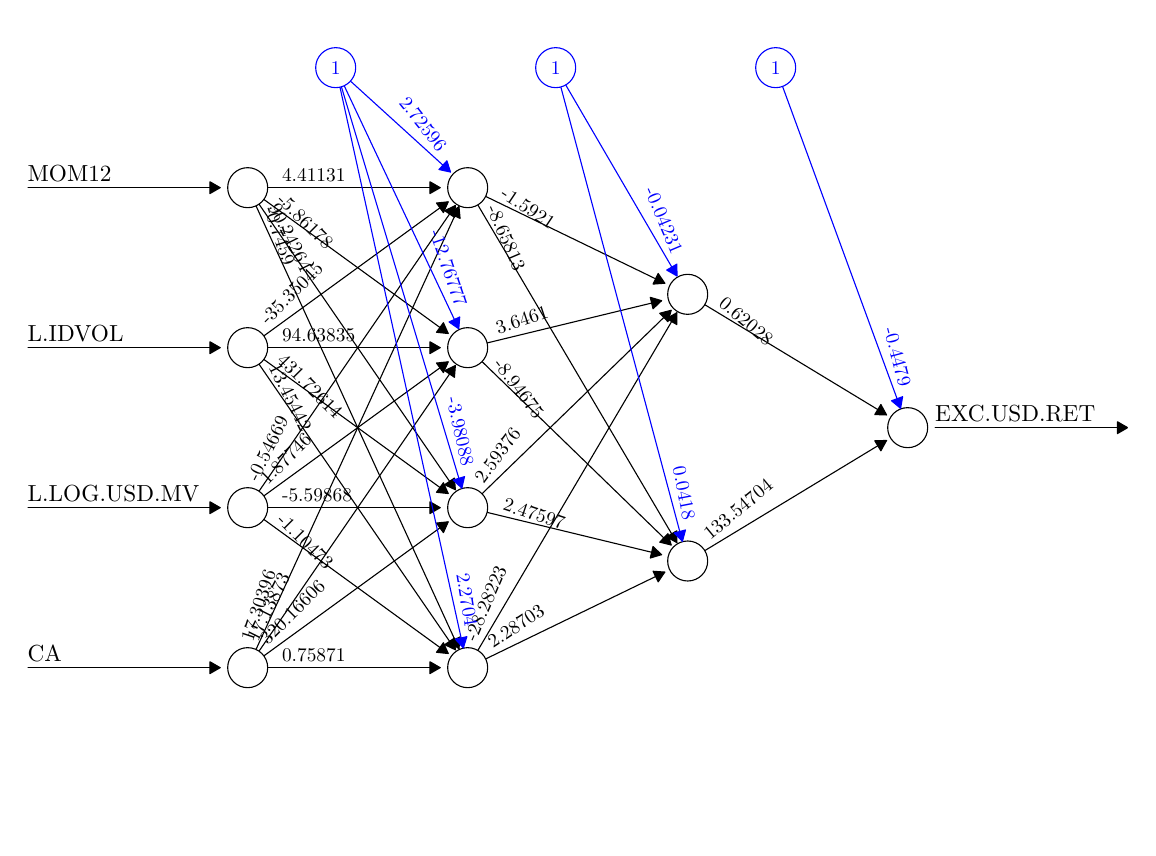
\begin{tikzpicture}[x=1pt,y=1pt]
\definecolor{fillColor}{RGB}{255,255,255}
\path[use as bounding box,fill=fillColor,fill opacity=0.00] (0,0) rectangle (397.48,289.08);
\begin{scope}
\path[clip] (  0.00,  0.00) rectangle (397.48,289.08);
\definecolor{drawColor}{RGB}{0,0,0}

\path[draw=drawColor,line width= 0.4pt,line join=round,line cap=round] ( 79.50, 57.82) --
	(149.06, 57.82);
\definecolor{fillColor}{RGB}{0,0,0}

\path[draw=drawColor,line width= 0.4pt,line join=round,line cap=round,fill=fillColor] (145.36, 55.68) --
	(149.06, 57.82) --
	(145.36, 59.95) --
	cycle;

\node[text=drawColor,anchor=base west,inner sep=0pt, outer sep=0pt, scale=  0.70] at ( 91.92, 59.95) {0.75871};
\end{scope}
\begin{scope}
\path[clip] (  0.00,  0.00) rectangle (397.48,289.08);
\definecolor{drawColor}{RGB}{0,0,0}

\path[draw=drawColor,line width= 0.4pt,line join=round,line cap=round] ( 79.50, 57.82) --
	(151.97,110.52);
\definecolor{fillColor}{RGB}{0,0,0}

\path[draw=drawColor,line width= 0.4pt,line join=round,line cap=round,fill=fillColor] (150.23,106.62) --
	(151.97,110.52) --
	(147.72,110.07) --
	cycle;

\node[text=drawColor,rotate= 45.00,anchor=base west,inner sep=0pt, outer sep=0pt, scale=  0.70] at ( 86.77, 65.71) {320.16606};
\end{scope}
\begin{scope}
\path[clip] (  0.00,  0.00) rectangle (397.48,289.08);
\definecolor{drawColor}{RGB}{0,0,0}

\path[draw=drawColor,line width= 0.4pt,line join=round,line cap=round] ( 79.50, 57.82) --
	(154.55,166.98);
\definecolor{fillColor}{RGB}{0,0,0}

\path[draw=drawColor,line width= 0.4pt,line join=round,line cap=round,fill=fillColor] (154.21,162.73) --
	(154.55,166.98) --
	(150.70,165.15) --
	cycle;

\node[text=drawColor,rotate= 63.43,anchor=base west,inner sep=0pt, outer sep=0pt, scale=  0.70] at ( 83.14, 66.85) {17.13873};
\end{scope}
\begin{scope}
\path[clip] (  0.00,  0.00) rectangle (397.48,289.08);
\definecolor{drawColor}{RGB}{0,0,0}

\path[draw=drawColor,line width= 0.4pt,line join=round,line cap=round] ( 79.50, 57.82) --
	(155.85,224.41);
\definecolor{fillColor}{RGB}{0,0,0}

\path[draw=drawColor,line width= 0.4pt,line join=round,line cap=round,fill=fillColor] (156.25,220.16) --
	(155.85,224.41) --
	(152.37,221.94) --
	cycle;

\node[text=drawColor,rotate= 71.57,anchor=base west,inner sep=0pt, outer sep=0pt, scale=  0.70] at ( 81.40, 67.06) {17.30396};
\end{scope}
\begin{scope}
\path[clip] (  0.00,  0.00) rectangle (397.48,289.08);
\definecolor{drawColor}{RGB}{0,0,0}

\path[draw=drawColor,line width= 0.4pt,line join=round,line cap=round] ( -0.00, 57.82) --
	( 69.56, 57.82);
\definecolor{fillColor}{RGB}{0,0,0}

\path[draw=drawColor,line width= 0.4pt,line join=round,line cap=round,fill=fillColor] ( 65.86, 55.68) --
	( 69.56, 57.82) --
	( 65.86, 59.95) --
	cycle;

\node[text=drawColor,anchor=base west,inner sep=0pt, outer sep=0pt, scale=  0.84] at ( -0.00, 59.95) {CA};
\end{scope}
\begin{scope}
\path[clip] (  0.00,  0.00) rectangle (397.48,289.08);
\definecolor{drawColor}{RGB}{0,0,0}
\definecolor{fillColor}{RGB}{255,255,255}

\path[draw=drawColor,line width= 0.4pt,line join=round,line cap=round,fill=fillColor] ( 79.50, 57.82) circle (  7.23);

\path[draw=drawColor,line width= 0.4pt,line join=round,line cap=round] ( 79.50,115.63) --
	(151.97, 62.93);
\definecolor{fillColor}{RGB}{0,0,0}

\path[draw=drawColor,line width= 0.4pt,line join=round,line cap=round,fill=fillColor] (147.72, 63.37) --
	(151.97, 62.93) --
	(150.23, 66.83) --
	cycle;

\node[text=drawColor,rotate=-45.00,anchor=base west,inner sep=0pt, outer sep=0pt, scale=  0.70] at ( 89.79,110.75) {-1.10473};
\end{scope}
\begin{scope}
\path[clip] (  0.00,  0.00) rectangle (397.48,289.08);
\definecolor{drawColor}{RGB}{0,0,0}

\path[draw=drawColor,line width= 0.4pt,line join=round,line cap=round] ( 79.50,115.63) --
	(149.06,115.63);
\definecolor{fillColor}{RGB}{0,0,0}

\path[draw=drawColor,line width= 0.4pt,line join=round,line cap=round,fill=fillColor] (145.36,113.50) --
	(149.06,115.63) --
	(145.36,117.77) --
	cycle;

\node[text=drawColor,anchor=base west,inner sep=0pt, outer sep=0pt, scale=  0.70] at ( 91.92,117.77) {-5.59868};
\end{scope}
\begin{scope}
\path[clip] (  0.00,  0.00) rectangle (397.48,289.08);
\definecolor{drawColor}{RGB}{0,0,0}

\path[draw=drawColor,line width= 0.4pt,line join=round,line cap=round] ( 79.50,115.63) --
	(151.97,168.34);
\definecolor{fillColor}{RGB}{0,0,0}

\path[draw=drawColor,line width= 0.4pt,line join=round,line cap=round,fill=fillColor] (150.23,164.44) --
	(151.97,168.34) --
	(147.72,167.89) --
	cycle;

\node[text=drawColor,rotate= 45.00,anchor=base west,inner sep=0pt, outer sep=0pt, scale=  0.70] at ( 86.77,123.53) {1.87746};
\end{scope}
\begin{scope}
\path[clip] (  0.00,  0.00) rectangle (397.48,289.08);
\definecolor{drawColor}{RGB}{0,0,0}

\path[draw=drawColor,line width= 0.4pt,line join=round,line cap=round] ( 79.50,115.63) --
	(154.55,224.80);
\definecolor{fillColor}{RGB}{0,0,0}

\path[draw=drawColor,line width= 0.4pt,line join=round,line cap=round,fill=fillColor] (154.21,220.55) --
	(154.55,224.80) --
	(150.70,222.96) --
	cycle;

\node[text=drawColor,rotate= 63.43,anchor=base west,inner sep=0pt, outer sep=0pt, scale=  0.70] at ( 83.14,124.67) {-0.54669};
\end{scope}
\begin{scope}
\path[clip] (  0.00,  0.00) rectangle (397.48,289.08);
\definecolor{drawColor}{RGB}{0,0,0}

\path[draw=drawColor,line width= 0.4pt,line join=round,line cap=round] ( -0.00,115.63) --
	( 69.56,115.63);
\definecolor{fillColor}{RGB}{0,0,0}

\path[draw=drawColor,line width= 0.4pt,line join=round,line cap=round,fill=fillColor] ( 65.86,113.50) --
	( 69.56,115.63) --
	( 65.86,117.77) --
	cycle;

\node[text=drawColor,anchor=base west,inner sep=0pt, outer sep=0pt, scale=  0.84] at ( -0.00,117.77) {L.LOG.USD.MV};
\end{scope}
\begin{scope}
\path[clip] (  0.00,  0.00) rectangle (397.48,289.08);
\definecolor{drawColor}{RGB}{0,0,0}
\definecolor{fillColor}{RGB}{255,255,255}

\path[draw=drawColor,line width= 0.4pt,line join=round,line cap=round,fill=fillColor] ( 79.50,115.63) circle (  7.23);

\path[draw=drawColor,line width= 0.4pt,line join=round,line cap=round] ( 79.50,173.45) --
	(154.55, 64.28);
\definecolor{fillColor}{RGB}{0,0,0}

\path[draw=drawColor,line width= 0.4pt,line join=round,line cap=round,fill=fillColor] (150.70, 66.12) --
	(154.55, 64.28) --
	(154.21, 68.53) --
	cycle;

\node[text=drawColor,rotate=-63.43,anchor=base west,inner sep=0pt, outer sep=0pt, scale=  0.70] at ( 86.96,166.32) {13.45442};
\end{scope}
\begin{scope}
\path[clip] (  0.00,  0.00) rectangle (397.48,289.08);
\definecolor{drawColor}{RGB}{0,0,0}

\path[draw=drawColor,line width= 0.4pt,line join=round,line cap=round] ( 79.50,173.45) --
	(151.97,120.74);
\definecolor{fillColor}{RGB}{0,0,0}

\path[draw=drawColor,line width= 0.4pt,line join=round,line cap=round,fill=fillColor] (147.72,121.19) --
	(151.97,120.74) --
	(150.23,124.64) --
	cycle;

\node[text=drawColor,rotate=-45.00,anchor=base west,inner sep=0pt, outer sep=0pt, scale=  0.70] at ( 89.79,168.57) {431.72614};
\end{scope}
\begin{scope}
\path[clip] (  0.00,  0.00) rectangle (397.48,289.08);
\definecolor{drawColor}{RGB}{0,0,0}

\path[draw=drawColor,line width= 0.4pt,line join=round,line cap=round] ( 79.50,173.45) --
	(149.06,173.45);
\definecolor{fillColor}{RGB}{0,0,0}

\path[draw=drawColor,line width= 0.4pt,line join=round,line cap=round,fill=fillColor] (145.36,171.31) --
	(149.06,173.45) --
	(145.36,175.58) --
	cycle;

\node[text=drawColor,anchor=base west,inner sep=0pt, outer sep=0pt, scale=  0.70] at ( 91.92,175.58) {94.63835};
\end{scope}
\begin{scope}
\path[clip] (  0.00,  0.00) rectangle (397.48,289.08);
\definecolor{drawColor}{RGB}{0,0,0}

\path[draw=drawColor,line width= 0.4pt,line join=round,line cap=round] ( 79.50,173.45) --
	(151.97,226.15);
\definecolor{fillColor}{RGB}{0,0,0}

\path[draw=drawColor,line width= 0.4pt,line join=round,line cap=round,fill=fillColor] (150.23,222.25) --
	(151.97,226.15) --
	(147.72,225.71) --
	cycle;

\node[text=drawColor,rotate= 45.00,anchor=base west,inner sep=0pt, outer sep=0pt, scale=  0.70] at ( 86.77,181.34) {-35.35045};
\end{scope}
\begin{scope}
\path[clip] (  0.00,  0.00) rectangle (397.48,289.08);
\definecolor{drawColor}{RGB}{0,0,0}

\path[draw=drawColor,line width= 0.4pt,line join=round,line cap=round] ( -0.00,173.45) --
	( 69.56,173.45);
\definecolor{fillColor}{RGB}{0,0,0}

\path[draw=drawColor,line width= 0.4pt,line join=round,line cap=round,fill=fillColor] ( 65.86,171.31) --
	( 69.56,173.45) --
	( 65.86,175.58) --
	cycle;

\node[text=drawColor,anchor=base west,inner sep=0pt, outer sep=0pt, scale=  0.84] at ( -0.00,175.58) {L.IDVOL};
\end{scope}
\begin{scope}
\path[clip] (  0.00,  0.00) rectangle (397.48,289.08);
\definecolor{drawColor}{RGB}{0,0,0}
\definecolor{fillColor}{RGB}{255,255,255}

\path[draw=drawColor,line width= 0.4pt,line join=round,line cap=round,fill=fillColor] ( 79.50,173.45) circle (  7.23);

\path[draw=drawColor,line width= 0.4pt,line join=round,line cap=round] ( 79.50,231.26) --
	(155.85, 64.67);
\definecolor{fillColor}{RGB}{0,0,0}

\path[draw=drawColor,line width= 0.4pt,line join=round,line cap=round,fill=fillColor] (152.37, 67.14) --
	(155.85, 64.67) --
	(156.25, 68.92) --
	cycle;

\node[text=drawColor,rotate=-71.57,anchor=base west,inner sep=0pt, outer sep=0pt, scale=  0.70] at ( 85.45,223.37) {-0.7459};
\end{scope}
\begin{scope}
\path[clip] (  0.00,  0.00) rectangle (397.48,289.08);
\definecolor{drawColor}{RGB}{0,0,0}

\path[draw=drawColor,line width= 0.4pt,line join=round,line cap=round] ( 79.50,231.26) --
	(154.55,122.10);
\definecolor{fillColor}{RGB}{0,0,0}

\path[draw=drawColor,line width= 0.4pt,line join=round,line cap=round,fill=fillColor] (150.70,123.93) --
	(154.55,122.10) --
	(154.21,126.35) --
	cycle;

\node[text=drawColor,rotate=-63.43,anchor=base west,inner sep=0pt, outer sep=0pt, scale=  0.70] at ( 86.96,224.14) {90.24264};
\end{scope}
\begin{scope}
\path[clip] (  0.00,  0.00) rectangle (397.48,289.08);
\definecolor{drawColor}{RGB}{0,0,0}

\path[draw=drawColor,line width= 0.4pt,line join=round,line cap=round] ( 79.50,231.26) --
	(151.97,178.56);
\definecolor{fillColor}{RGB}{0,0,0}

\path[draw=drawColor,line width= 0.4pt,line join=round,line cap=round,fill=fillColor] (147.72,179.01) --
	(151.97,178.56) --
	(150.23,182.46) --
	cycle;

\node[text=drawColor,rotate=-45.00,anchor=base west,inner sep=0pt, outer sep=0pt, scale=  0.70] at ( 89.79,226.39) {-5.86178};
\end{scope}
\begin{scope}
\path[clip] (  0.00,  0.00) rectangle (397.48,289.08);
\definecolor{drawColor}{RGB}{0,0,0}

\path[draw=drawColor,line width= 0.4pt,line join=round,line cap=round] ( 79.50,231.26) --
	(149.06,231.26);
\definecolor{fillColor}{RGB}{0,0,0}

\path[draw=drawColor,line width= 0.4pt,line join=round,line cap=round,fill=fillColor] (145.36,229.13) --
	(149.06,231.26) --
	(145.36,233.40) --
	cycle;

\node[text=drawColor,anchor=base west,inner sep=0pt, outer sep=0pt, scale=  0.70] at ( 91.92,233.40) {4.41131};
\end{scope}
\begin{scope}
\path[clip] (  0.00,  0.00) rectangle (397.48,289.08);
\definecolor{drawColor}{RGB}{0,0,0}

\path[draw=drawColor,line width= 0.4pt,line join=round,line cap=round] ( -0.00,231.26) --
	( 69.56,231.26);
\definecolor{fillColor}{RGB}{0,0,0}

\path[draw=drawColor,line width= 0.4pt,line join=round,line cap=round,fill=fillColor] ( 65.86,229.13) --
	( 69.56,231.26) --
	( 65.86,233.40) --
	cycle;

\node[text=drawColor,anchor=base west,inner sep=0pt, outer sep=0pt, scale=  0.84] at ( -0.00,233.40) {MOM12};
\end{scope}
\begin{scope}
\path[clip] (  0.00,  0.00) rectangle (397.48,289.08);
\definecolor{drawColor}{RGB}{0,0,0}
\definecolor{fillColor}{RGB}{255,255,255}

\path[draw=drawColor,line width= 0.4pt,line join=round,line cap=round,fill=fillColor] ( 79.50,231.26) circle (  7.23);

\path[draw=drawColor,line width= 0.4pt,line join=round,line cap=round] (158.99, 57.82) --
	(230.22, 92.35);
\definecolor{fillColor}{RGB}{0,0,0}

\path[draw=drawColor,line width= 0.4pt,line join=round,line cap=round,fill=fillColor] (227.83, 88.82) --
	(230.22, 92.35) --
	(225.97, 92.66) --
	cycle;

\node[text=drawColor,rotate= 33.69,anchor=base west,inner sep=0pt, outer sep=0pt, scale=  0.70] at (168.15, 64.60) {2.28703};
\end{scope}
\begin{scope}
\path[clip] (  0.00,  0.00) rectangle (397.48,289.08);
\definecolor{drawColor}{RGB}{0,0,0}

\path[draw=drawColor,line width= 0.4pt,line join=round,line cap=round] (158.99, 57.82) --
	(234.58,186.08);
\definecolor{fillColor}{RGB}{0,0,0}

\path[draw=drawColor,line width= 0.4pt,line join=round,line cap=round,fill=fillColor] (234.54,181.81) --
	(234.58,186.08) --
	(230.86,183.98) --
	cycle;

\node[text=drawColor,rotate= 66.80,anchor=base west,inner sep=0pt, outer sep=0pt, scale=  0.70] at (161.93, 66.96) {-28.28223};
\end{scope}
\begin{scope}
\path[clip] (  0.00,  0.00) rectangle (397.48,289.08);
\definecolor{drawColor}{RGB}{0,0,0}
\definecolor{fillColor}{RGB}{255,255,255}

\path[draw=drawColor,line width= 0.4pt,line join=round,line cap=round,fill=fillColor] (158.99, 57.82) circle (  7.23);

\path[draw=drawColor,line width= 0.4pt,line join=round,line cap=round] (158.99,115.63) --
	(229.06, 98.65);
\definecolor{fillColor}{RGB}{0,0,0}

\path[draw=drawColor,line width= 0.4pt,line join=round,line cap=round,fill=fillColor] (224.97, 97.44) --
	(229.06, 98.65) --
	(225.97,101.59) --
	cycle;

\node[text=drawColor,rotate=-18.43,anchor=base west,inner sep=0pt, outer sep=0pt, scale=  0.70] at (171.45,114.80) {2.47597};
\end{scope}
\begin{scope}
\path[clip] (  0.00,  0.00) rectangle (397.48,289.08);
\definecolor{drawColor}{RGB}{0,0,0}

\path[draw=drawColor,line width= 0.4pt,line join=round,line cap=round] (158.99,115.63) --
	(232.53,186.94);
\definecolor{fillColor}{RGB}{0,0,0}

\path[draw=drawColor,line width= 0.4pt,line join=round,line cap=round,fill=fillColor] (231.36,182.83) --
	(232.53,186.94) --
	(228.39,185.90) --
	cycle;

\node[text=drawColor,rotate= 53.13,anchor=base west,inner sep=0pt, outer sep=0pt, scale=  0.70] at (164.74,124.14) {2.59376};
\end{scope}
\begin{scope}
\path[clip] (  0.00,  0.00) rectangle (397.48,289.08);
\definecolor{drawColor}{RGB}{0,0,0}
\definecolor{fillColor}{RGB}{255,255,255}

\path[draw=drawColor,line width= 0.4pt,line join=round,line cap=round,fill=fillColor] (158.99,115.63) circle (  7.23);

\path[draw=drawColor,line width= 0.4pt,line join=round,line cap=round] (158.99,173.45) --
	(232.53,102.14);
\definecolor{fillColor}{RGB}{0,0,0}

\path[draw=drawColor,line width= 0.4pt,line join=round,line cap=round,fill=fillColor] (228.39,103.18) --
	(232.53,102.14) --
	(231.36,106.25) --
	cycle;

\node[text=drawColor,rotate=-53.13,anchor=base west,inner sep=0pt, outer sep=0pt, scale=  0.70] at (168.15,167.50) {-8.94675};
\end{scope}
\begin{scope}
\path[clip] (  0.00,  0.00) rectangle (397.48,289.08);
\definecolor{drawColor}{RGB}{0,0,0}

\path[draw=drawColor,line width= 0.4pt,line join=round,line cap=round] (158.99,173.45) --
	(229.06,190.43);
\definecolor{fillColor}{RGB}{0,0,0}

\path[draw=drawColor,line width= 0.4pt,line join=round,line cap=round,fill=fillColor] (225.97,187.49) --
	(229.06,190.43) --
	(224.97,191.64) --
	cycle;

\node[text=drawColor,rotate= 18.43,anchor=base west,inner sep=0pt, outer sep=0pt, scale=  0.70] at (170.10,178.33) {3.6461};
\end{scope}
\begin{scope}
\path[clip] (  0.00,  0.00) rectangle (397.48,289.08);
\definecolor{drawColor}{RGB}{0,0,0}
\definecolor{fillColor}{RGB}{255,255,255}

\path[draw=drawColor,line width= 0.4pt,line join=round,line cap=round,fill=fillColor] (158.99,173.45) circle (  7.23);

\path[draw=drawColor,line width= 0.4pt,line join=round,line cap=round] (158.99,231.26) --
	(234.58,103.00);
\definecolor{fillColor}{RGB}{0,0,0}

\path[draw=drawColor,line width= 0.4pt,line join=round,line cap=round,fill=fillColor] (230.86,105.10) --
	(234.58,103.00) --
	(234.54,107.27) --
	cycle;

\node[text=drawColor,rotate=-66.80,anchor=base west,inner sep=0pt, outer sep=0pt, scale=  0.70] at (165.85,223.80) {-8.65813};
\end{scope}
\begin{scope}
\path[clip] (  0.00,  0.00) rectangle (397.48,289.08);
\definecolor{drawColor}{RGB}{0,0,0}

\path[draw=drawColor,line width= 0.4pt,line join=round,line cap=round] (158.99,231.26) --
	(230.22,196.73);
\definecolor{fillColor}{RGB}{0,0,0}

\path[draw=drawColor,line width= 0.4pt,line join=round,line cap=round,fill=fillColor] (225.97,196.42) --
	(230.22,196.73) --
	(227.83,200.26) --
	cycle;

\node[text=drawColor,rotate=-33.69,anchor=base west,inner sep=0pt, outer sep=0pt, scale=  0.70] at (170.51,228.03) {-1.5921};
\end{scope}
\begin{scope}
\path[clip] (  0.00,  0.00) rectangle (397.48,289.08);
\definecolor{drawColor}{RGB}{0,0,0}
\definecolor{fillColor}{RGB}{255,255,255}

\path[draw=drawColor,line width= 0.4pt,line join=round,line cap=round,fill=fillColor] (158.99,231.26) circle (  7.23);

\path[draw=drawColor,line width= 0.4pt,line join=round,line cap=round] (238.49, 96.36) --
	(310.35,139.91);
\definecolor{fillColor}{RGB}{0,0,0}

\path[draw=drawColor,line width= 0.4pt,line join=round,line cap=round,fill=fillColor] (308.30,136.17) --
	(310.35,139.91) --
	(306.09,139.82) --
	cycle;

\node[text=drawColor,rotate= 39.81,anchor=base west,inner sep=0pt, outer sep=0pt, scale=  0.70] at (246.67,103.78) {133.54704};
\end{scope}
\begin{scope}
\path[clip] (  0.00,  0.00) rectangle (397.48,289.08);
\definecolor{drawColor}{RGB}{0,0,0}
\definecolor{fillColor}{RGB}{255,255,255}

\path[draw=drawColor,line width= 0.4pt,line join=round,line cap=round,fill=fillColor] (238.49, 96.36) circle (  7.23);

\path[draw=drawColor,line width= 0.4pt,line join=round,line cap=round] (238.49,192.72) --
	(310.35,149.17);
\definecolor{fillColor}{RGB}{0,0,0}

\path[draw=drawColor,line width= 0.4pt,line join=round,line cap=round,fill=fillColor] (306.09,149.26) --
	(310.35,149.17) --
	(308.30,152.91) --
	cycle;

\node[text=drawColor,rotate=-39.81,anchor=base west,inner sep=0pt, outer sep=0pt, scale=  0.70] at (249.40,188.58) {0.62028};
\end{scope}
\begin{scope}
\path[clip] (  0.00,  0.00) rectangle (397.48,289.08);
\definecolor{drawColor}{RGB}{0,0,0}
\definecolor{fillColor}{RGB}{255,255,255}

\path[draw=drawColor,line width= 0.4pt,line join=round,line cap=round,fill=fillColor] (238.49,192.72) circle (  7.23);

\path[draw=drawColor,line width= 0.4pt,line join=round,line cap=round] (327.93,144.54) --
	(397.48,144.54);
\definecolor{fillColor}{RGB}{0,0,0}

\path[draw=drawColor,line width= 0.4pt,line join=round,line cap=round,fill=fillColor] (393.79,142.41) --
	(397.48,144.54) --
	(393.79,146.67) --
	cycle;

\node[text=drawColor,anchor=base west,inner sep=0pt, outer sep=0pt, scale=  0.84] at (327.93,146.67) {EXC.USD.RET};
\end{scope}
\begin{scope}
\path[clip] (  0.00,  0.00) rectangle (397.48,289.08);
\definecolor{drawColor}{RGB}{0,0,0}
\definecolor{fillColor}{RGB}{255,255,255}

\path[draw=drawColor,line width= 0.4pt,line join=round,line cap=round,fill=fillColor] (317.99,144.54) circle (  7.23);
\definecolor{drawColor}{RGB}{0,0,255}

\path[draw=drawColor,line width= 0.4pt,line join=round,line cap=round] (111.30,274.63) --
	(157.42, 64.95);
\definecolor{fillColor}{RGB}{0,0,255}

\path[draw=drawColor,line width= 0.4pt,line join=round,line cap=round,fill=fillColor] (154.55, 68.10) --
	(157.42, 64.95) --
	(158.71, 69.02) --
	cycle;

\node[text=drawColor,rotate=-80.91,anchor=base east,inner sep=0pt, outer sep=0pt, scale=  0.70] at (157.96, 72.43) {2.2704};
\end{scope}
\begin{scope}
\path[clip] (  0.00,  0.00) rectangle (397.48,289.08);
\definecolor{drawColor}{RGB}{0,0,255}

\path[draw=drawColor,line width= 0.4pt,line join=round,line cap=round] (111.30,274.63) --
	(156.88,122.69);
\definecolor{fillColor}{RGB}{0,0,255}

\path[draw=drawColor,line width= 0.4pt,line join=round,line cap=round,fill=fillColor] (153.77,125.62) --
	(156.88,122.69) --
	(157.86,126.85) --
	cycle;

\node[text=drawColor,rotate=-77.69,anchor=base east,inner sep=0pt, outer sep=0pt, scale=  0.70] at (156.84,130.21) {-3.98088};
\end{scope}
\begin{scope}
\path[clip] (  0.00,  0.00) rectangle (397.48,289.08);
\definecolor{drawColor}{RGB}{0,0,255}

\path[draw=drawColor,line width= 0.4pt,line join=round,line cap=round] (111.30,274.63) --
	(155.77,180.28);
\definecolor{fillColor}{RGB}{0,0,255}

\path[draw=drawColor,line width= 0.4pt,line join=round,line cap=round,fill=fillColor] (152.26,182.72) --
	(155.77,180.28) --
	(156.13,184.54) --
	cycle;

\node[text=drawColor,rotate=-71.08,anchor=base east,inner sep=0pt, outer sep=0pt, scale=  0.70] at (154.57,187.81) {-12.76777};
\end{scope}
\begin{scope}
\path[clip] (  0.00,  0.00) rectangle (397.48,289.08);
\definecolor{drawColor}{RGB}{0,0,255}

\path[draw=drawColor,line width= 0.4pt,line join=round,line cap=round] (111.30,274.63) --
	(152.79,236.91);
\definecolor{fillColor}{RGB}{0,0,255}

\path[draw=drawColor,line width= 0.4pt,line join=round,line cap=round,fill=fillColor] (148.62,237.81) --
	(152.79,236.91) --
	(151.49,240.97) --
	cycle;

\node[text=drawColor,rotate=-51.34,anchor=base east,inner sep=0pt, outer sep=0pt, scale=  0.70] at (148.24,243.88) {2.72596};
\end{scope}
\begin{scope}
\path[clip] (  0.00,  0.00) rectangle (397.48,289.08);
\definecolor{drawColor}{RGB}{0,0,255}
\definecolor{fillColor}{RGB}{255,255,255}

\path[draw=drawColor,line width= 0.4pt,line join=round,line cap=round,fill=fillColor] (111.30,274.63) circle (  7.23);

\node[text=drawColor,anchor=base,inner sep=0pt, outer sep=0pt, scale=  0.70] at (111.30,272.22) {1};

\path[draw=drawColor,line width= 0.4pt,line join=round,line cap=round] (190.79,274.63) --
	(236.59,103.45);
\definecolor{fillColor}{RGB}{0,0,255}

\path[draw=drawColor,line width= 0.4pt,line join=round,line cap=round,fill=fillColor] (233.58,106.47) --
	(236.59,103.45) --
	(237.70,107.58) --
	cycle;

\node[text=drawColor,rotate=-78.99,anchor=base east,inner sep=0pt, outer sep=0pt, scale=  0.70] at (236.79,110.96) {0.0418};
\end{scope}
\begin{scope}
\path[clip] (  0.00,  0.00) rectangle (397.48,289.08);
\definecolor{drawColor}{RGB}{0,0,255}

\path[draw=drawColor,line width= 0.4pt,line join=round,line cap=round] (190.79,274.63) --
	(234.62,199.37);
\definecolor{fillColor}{RGB}{0,0,255}

\path[draw=drawColor,line width= 0.4pt,line join=round,line cap=round,fill=fillColor] (230.91,201.49) --
	(234.62,199.37) --
	(234.60,203.64) --
	cycle;

\node[text=drawColor,rotate=-67.05,anchor=base east,inner sep=0pt, outer sep=0pt, scale=  0.70] at (232.71,206.86) {-0.04231};
\end{scope}
\begin{scope}
\path[clip] (  0.00,  0.00) rectangle (397.48,289.08);
\definecolor{drawColor}{RGB}{0,0,255}
\definecolor{fillColor}{RGB}{255,255,255}

\path[draw=drawColor,line width= 0.4pt,line join=round,line cap=round,fill=fillColor] (190.79,274.63) circle (  7.23);

\node[text=drawColor,anchor=base,inner sep=0pt, outer sep=0pt, scale=  0.70] at (190.79,272.22) {1};

\path[draw=drawColor,line width= 0.4pt,line join=round,line cap=round] (270.29,274.63) --
	(315.43,151.52);
\definecolor{fillColor}{RGB}{0,0,255}

\path[draw=drawColor,line width= 0.4pt,line join=round,line cap=round,fill=fillColor] (312.15,154.26) --
	(315.43,151.52) --
	(316.16,155.73) --
	cycle;

\node[text=drawColor,rotate=-75.07,anchor=base east,inner sep=0pt, outer sep=0pt, scale=  0.70] at (314.93,159.06) {-0.4479};
\end{scope}
\begin{scope}
\path[clip] (  0.00,  0.00) rectangle (397.48,289.08);
\definecolor{drawColor}{RGB}{0,0,255}
\definecolor{fillColor}{RGB}{255,255,255}

\path[draw=drawColor,line width= 0.4pt,line join=round,line cap=round,fill=fillColor] (270.29,274.63) circle (  7.23);

\node[text=drawColor,anchor=base,inner sep=0pt, outer sep=0pt, scale=  0.70] at (270.29,272.22) {1};
\end{scope}
\end{tikzpicture}

\label{plot:NN}
\end{figure}

One of the first things the user has to decide while training a neural network is the architecture of the model. This study focuses on feedforward neural networks which consist of the input layer, hidden layers and an output layer. The input layer consists of the predictive variables whereas the output layer produces the final prediction. In between there exist 1 to N hidden layers. Hidden layers again consist of so-called neurons. Similar to the number of hidden layers, the user has to also decide the number of neurons in each of the hidden layers. Number of the hidden layers is often referred as the deepness of the model whereas number of the neurons in each hidden layer is referred as the width of the model. \par

While a lot of previous literature simultaneously examines multiple different architectural forms, due to computing capacity in this study only one architecture will be examined \citep{guetal, HANAUER2023, TOBEK2021100588}. The neural network architecture chosen for this study has two hidden layers. The first hidden layer has 16 neurons and following the common geometric pyramid rule second hidden layer has 8 neurons. Rather shallow and narrow architecture is chosen because they usually perform better with smaller datasets \citep{guetal}. In order to improve and fasten the converging of the model batch normalization is implemented between all layers. \par

The idea of the neural network is that each neuron, using weights and biases terms, aggregates information from the previous layer and subsequently feeds the information to the activations function. The neural network model used in this study is fully connected, meaning that each neuron is connected to all neurons in the previous layer. The output of the activation function will be the input for the next layer. The neural network model is trained by optimizing these weights and bias terms. There exist many options for the activation function, which is again one choice the user has to make. The activation function used in this study is rectified linear unit \par

\begin{equation}
\label{ReLU}
ReLU(x) = max(0, x)
\end{equation}

Since the model is trained for a regression task final neuron in the output layer has a different activation function than the neurons in the hidden layers. The activation function for the output neuron is a linear function. \par

As mentioned neural networks include numerous hyperparameters that can be optimized during the training of the model. Training neural networks is computationally demanding. Due to limited computing capacity, hyperparameters are not optimized in this study, but predefined values are used. Hyperparameters and their values are presented in Table \ref{table:Hyperparameters}. Additionally, to further limit the computational demand and simultaneously avoid overfitting early stopping algorithm is applied. Early stopping is implemented so that training of the model is terminated after five epochs where the loss function value does not reduce for the validation set. Instead of inserting the whole dataset into the model at once, data is inserted into the model in smaller subsamples so-called batches. Epoch on the other hand measures how many times the whole dataset is run through the model. \par

Neural networks learn by adjusting weights to the direction of the gradient. This is done in repetitive iterations. In each iteration size of the change is defined by a hyperparameter called learning rate. Since the learning rate is a hyperparameter it needs input from the user. It can also be optimized. Setting the correct learning rate is crucial since too big learning rate might prevent the algorithm from converging to the optimal solution, but too small learning rate makes converging slow. For the above-described reasons learning rate is not optimized in this study, but using a learning rate scheduler it is adjusted during the training of the model. In order to ensure efficient training learning rate is set to 0.01 at the beginning of the training and after ten epochs learning rate will be multiplied by 0.9 in each epoch. \par

Neural networks are also sensitive to the weight initialization, where the initial weights are set which the model starts to optimize. Depending on the initialization of the weights neural networks can converge to different results. To reduce model variance caused by this, an ensemble method is applied. An ensemble is implemented by training five separate models with different initial weights. The final prediction will be then the average of the predictions of the five models. \par

\subsection{Prediction performance evaluation}\label{PredictionPerformanceEvaluation}

This study will evaluate machine learning methods from two perspectives. Models are evaluated based on their predictive accuracy and their potential economic profitability. The profitability of the models is evaluated by backtesting portfolios that are constructed based on the stock return prediction of different models. Prediction accuracy is on the other hand evaluated by a set of statistical tests which are described in more detail below. This allows us to evaluate the relation between predicted and realized excess returns. \par

The first perspective that machine learning models are evaluated is based on their prediction accuracy. Prediction accuracy will be evaluated using out-of-sample $R^{2}_{oos}$ and \citet{Diebold1995} tests. Two out-of-sample $R^{2}$ figures are considered. Traditional out-of-sample $R^{2}$ uses historical mean return as the benchmark estimation. Traditional out-of-sample $R^{2}$ is defined as \par

\begin{equation}
\label{eq:r2Trad}
R^{2}_{oos \ Trad.} = 1 - \frac{\sum^T_{t=1} \sum^N_{i=1} (r_{i, t} - \hat r_{i, t})^2}{ \sum^T_{t=1} \sum^N_{i=1} (r_{i, t} - \overline{r}_{i, t} )^2}
\end{equation}

where $r_{i, t}$ is the realized return of stock $i$ in month $t$, $\hat r_{i, t}$ is the predicted return of the same stock for month $i$ and $\overline{r}_{i, t}$ is the historical mean return of the same stock excluding month $i$. Nevertheless, \citet{guetal} argue that the historical mean return is so noisy estimator that it underperforms compared to a static estimation of zero and therefore artificially improves the out-of-sample $R^{2}$. Instead, they propose an alternative out-of-sample $R^{2}$ measure where the squared sum of returns in the denominator is not demeaned. \par

\begin{equation}
\label{eq:r2}
R^{2}_{oos} = 1 - \frac{\sum^T_{t=1} \sum^N_{i=1} (r_{i, t} - \hat r_{i, t})^2}{ \sum^T_{t=1} \sum^N_{i=1} r^2_{i, t}}
\end{equation}

$R^2$ presents the prediction accuracy as a single figure, whereas \citet{Diebold1995} test allows for pairwise comparison of different models. Diebold-Mariano value is calculated as \par

\begin{equation}
\label{eq:Diebold-Mariano}
\begin{split}
 d_{12, t} 			& = \ \frac{1}{N_{t}}  \sum^N_{i=1}((r_{i, t} - \hat r_{i, t, 1})^2 - (r_{i, t} - \hat r_{i, t, 2})^2) \\
\overline{d}_{12} 	& = \ \frac{1}{T} \sum^T_{t=1} d_{12, t} \\
DM_{12} 			& = \ \frac{\overline{d}_{12}}{\hat \sigma_{d_{12}}} \\
\end{split}
\end{equation}

where $\hat r_{i, t, 1}$ is the return prediction of first model for company $i$ at time $t$, $\hat r_{i, t, 1}$ is the return prediction of the second model  for company $i$ at time $t$ and $N_t$ is the number of observations in the prediction period $t$. Therefore, $d_{12, t}$ is a time series of differences in average squared prediction errors between model $1$ and model $2$. Then $\overline{d}_{12}$ is the time series mean of $d_{12, t}$ and $\hat \sigma_{d_{12}}$ is the \citet{Newey1987} standard error of $d_{12, t}$. \citet{Diebold1995} test allows us to estimate the statistical significance of the prediction accuracy of two models. Under the assumption that there do not exist differences in prediction accuracy between models Diebold-Mariano statistic follows the normal distribution with a mean of $0$ and standard deviation of $1$, $DM \sim \mathcal{N}(0,\, 1)$. The significance of the difference is reported both for traditional $5\%$ level as well as for 3-way comparisons with Bonferroni adjustment. \par

In the spirit of \citet{Lewellen2015} expected returns are also estimated by regressing realized returns with the expected returns. This regression follows \par

\begin{equation}
\label{eq:realizedRegression}
r_{i, t} = \alpha + \beta_1 \hat r_{i, t}
\end{equation}

where $r_{i, t}$ is the realized return of company $i$ at time $t$ and $\hat r_{i, t}$ is the expected return of corresponding model for company $i$ at time $t$. For these regressions betas, $t$-statistics for betas and $R^2$ values will be reported. Ideally, the beta coefficient or the slope for the predicted return should be 1 and highly significant. The magnitude of the beta coefficients can provide information on possible over or undershooting of the models. \par

The second perspective that is evaluated is the economic profitability of the methods. Profitability is estimated via portfolio construction following the approach of \citet{Lewellen2015}. First expected returns are derived from each model. This process is introduced in more detail in the above subsections for each model. After obtaining the expected returns, each month all stocks are distributed to ten portfolios based on the magnitude of their expected return. Allocation is univariate and does not consider any other variables than the expected return of the stock for the next month. Even though models are trained only once a year, expected returns are re-calculated every month as the most recent available data is inserted into the model. Therefore, also the portfolio allocation is repeated monthly. Each month all stocks are allocated to one of the ten expected return portfolios, but to avoid the result being mainly driven by small stocks approach from \citet{HANAUER2023} is applied and the breakpoints for the allocation are calculated only from the large market value stocks. Large market value stocks are the biggest stocks that account for 90\% of the aggregated total market value of the respective month. \par

In addition to the ten expected return portfolios, for each method zero investment portfolio is formed. Zero investment, or long-short portfolio, is simply the spread between the return of the highest expected return portfolio and the return of the lowest expected return portfolio. Both value and equal-weighted returns will be reported for each portfolio including expected return and long-short portfolios. The performance of the machine learning portfolios is backtested and evaluated in multiple ways. For all expected return portfolios historical realized mean returns are reported together with Sharpe ratios. Sharpe ratio is defined as

\begin{equation}
\label{eq:SharpeRatio}
Sharpe \ Ratio = \frac{\overline{r}_i}{\sigma_i}
\end{equation}

where $\overline{r}_i$ is the time series average excess return of portfolio $i$ and $\sigma_i$ is the standard deviation of the excess returns of portfolio $i$. For long-short portfolios also maximum drawdown and maximum one-month loss will be reported. Maximum one-month loss is simply the largest negative monthly return of each portfolio. Maximum drawdown is defined as \par

\begin{equation}
\label{eq:maxDD}
MaxDD = \max\limits_{0\leq t_1\leq t_2\leq T} (Y_{t_1} - Y_{t_2})
\end{equation}

where $Y_t$ stands for cumulative return from the beginning of the period until date $t$. In order to examine risk-adjusted returns long-short portfolio returns will be regressed against \citet{FAMA20151} six-factor model factors\footnotemark. From this regression alphas, which can be interpreted as the excess return that the models are able to generate and cannot be explained by the loadings in the six risk factors. Also, $t$-statistics for the alphas and $R^2$ values are reported. Regression formula for risk-adjusted performance \par

\begin{equation}
\label{eq:FFRegFormula}
\begin{split}
r_{t, m} = 	& \ \alpha+ \beta_{1} \ RMRF_{t} + \beta_{2} + \ SMB_{t} + \beta_{3} \ HML_{t} + \\
		&  \beta_{4} \ CMA_{t} +  \beta_{5} \ RMW_{t} + \beta_{6} \ MOM_{t} + \epsilon_{t}
\end{split}
\end{equation}

where $r_{t, m}$ is the return of long-short portfolio from model $m$ in time $t$, $RMRF$ is the excess market return, $SMB$ is the spread in the return between small market value stocks and large market value stocks, $HML$ is the spread in the return between high book-to-market value stocks and low book-to-market value stocks, $CMA$ is the spread in the return between conservatively investing stocks and aggressively investing stocks, $RMW$ is the spread in the return between stocks with robust profitability and stocks with weak profitability and $MOM$ is the between returns of stocks that had the highest return in period $t-1$ and the stocks that had the lowest return in period $t-1$. Factors are constructed from the same dataset as machine learning portfolios, except that the micro-cap stocks are not excluded. Construction of these factors is described in more detail in Section \ref{BenchmarkFactorsConstruction}. \par

\footnotetext{\citet{FAMA20151} introduced the five factor model. Factors used to regress machine learning portfolio returns include five-factor model factors and momentum factor from \citet{Carhart1997}.}

Finally, turnovers for the long-short portfolios are reported. In a real-world setting, investors usually are subject to some sort of trading cost. Even if the model generates excess returns but the monthly turnover remains large, it could lead to a situation where after counting for transaction costs more passive strategy would become more profitable. Therefore, turnover provides valuable information on the practical implementability of the constructed machine learning models. For month $t$ turnover is defined as \par

\begin{equation}
\label{eq:Turnover}
Turnover_t = \sum_{i=1}^{N_t}  \left ( \left | w_{i, t} - \frac{w_{i, t-1}(1 + r_{i, t})}{ \sum_{j=1}^{N_{t}} w_{j, t-1}(1 + r_{j, t})} \right | \right )
\end{equation}

where $N_t$ is number of companies in portfolio $j$ in month $t$ and $w_{i, t}$ is the weight of the company $i$ in portfolio $j$ after the reallocation. The latter part of the equation indicates the weight of the company $i$ right before the reallocation. It considers the change in weight of company $i$ due to the relative return in month $t$ compared to the return of the corresponding portfolio.

\subsection{Variable importance} \label{VariableImportance}

One challenge in dealing with various statistical methods is that they lack common metrics for explanatory inference. Many of the models have metrics for variable importance, but the comparability of these metrics can be questioned. Therefore, the approach of \citet{guetal} is implemented to define variable importance metrics for the model applied in this study. The approach consists of the following steps. First one variable at a time is set to zero. Then the reduced model is retrained and new predicted returns are derived using the reduced model. The process of training and predicting returns is identical to the reduced model as for the full model. After obtaining the predicted returns from the reduced model, out-of-sample $R^2$ values are calculated for these returns. Then change compared to out-of-sample $R^2$ of the full model is calculated. Finally, to obtain the relative variable importance metric, the sum of changes in out-of-sample $R^2$s is normalized to one within a model. The same process is applied to each variable and all models. \par

\subsection{Sample splitting} \label{SampleSplitting}

It is common while training machine learning models to split the data into three sets. The training set will be used as the name suggests to train the model. In case a machine learning model includes hyperparameters these can be optimized with a validation set. Finally, the true out-of-sample predictions can be performed for testing data. Because we want to mimic the situation and information set of an investor we have to take into consideration the time series nature of the data. \par

In stock return prediction literature it is common to split the data as described above, but considering the chronological order. For example \citet{Fieberg} use a rolling ten-year scheme where they first train the model using the first seven years of the data and then optimize hyperparameters using the last three years of the rolling window. Finally, they train the model with optimal hyperparameter initialization with a whole ten-year window to predict returns for the next year. \citet{guetal} use a slightly different approach. Instead of using a rolling window, they increase the training window size after each training period by one year. Common for these two approaches is that they both train the model only once a year. \par

\definecolor{Gray}{RGB}{160,160,160}
\definecolor{LightGray}{RGB}{191,191,191}
\begin{figure}[ht]
\centering
\caption[Sample splitting scheme]{\textbf{Sample splitting \textnormal{- Own source}}\\ Illustration sample splitting used in training of the machine learning models. Machine learning models are trained once a year and after each training model is used for the next 12 months to predict the stock returns. Each year training period is extended by 12 months. The training period is further split into training data and validation data randomly allocating 80\% of the data to the training set and 20\% of the data to the validation set. A validation set is used to optimize hyperparameters. The minimum length of the training period is 50 months.}
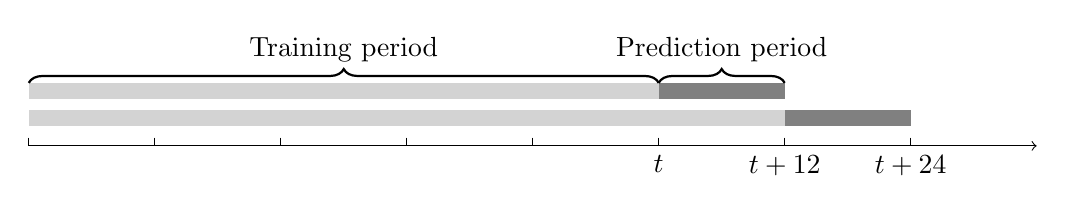
\begin{tikzpicture}
\draw[->] (0, 0) -- (12.8, 0);
\foreach \x in {0, 1.6,...,12.8}{
    \draw (\x cm, 3pt) -- (\x cm, 0pt);
} 
\fill[LightGray] (0, 0.8) rectangle (8, 0.6);
\fill[Gray] (8, 0.8) rectangle (9.6, 0.6);
\fill[LightGray] (0, 0.45) rectangle (9.6, 0.25);
\fill[Gray] (9.6, 0.45) rectangle (11.2, 0.25);

\draw [thick, decorate, decoration = {brace, amplitude = 5pt}] (0, 0.8)  -- +(8, 0) 
       node [black, midway, above = 4pt] {Training period};
\draw [thick, decorate, decoration = {brace, amplitude = 5pt}] (8, 0.8)  -- +(1.6, 0) 
       node [black, midway, above = 4pt] {Prediction period};
       
\node[anchor=north] at (8, 0) {$t$};
\node[anchor=north] at (9.6,0) {$t+12$};
\node[anchor=north] at (11.2, 0) {$t+24$};
\end{tikzpicture}
\label{plot:SampleSplitting}
\end{figure}

The sample splitting scheme applied in this study is slightly different from above described ones. The above-described approaches use disjoint time periods to mimic the out-of-sample setting in the hyperparameter optimization. In this study training and validation sets are separated from the testing data based on time. The approach is closer to the approach of \citet{guetal} in the sense that the training data window is increased each year. Nevertheless, the difference is that the data is distributed to training data and validation randomly instead of using the disjoint periods. The reason why this scheme is chosen is that we want to avoid the retraining of the model after the hyperparameter optimization which is necessary if the most recent data should be included in the model. The sample splitting scheme is illustrated in Figure \ref{plot:SampleSplitting}. \par

\begin{table}[ht]
\footnotesize
\caption[Hyperparameters]{\textbf{Hyperparameters \textnormal{- Own source}}\\ Table presents the hyperparameters that are either optimized or taken as fixed values. In case predefined values are used only one figure is indicated in the table. If hyperparameter is optimized set or list is displayed. FM stands for linear regression model, RF stands for random forest model and NN stands for neural networks model.  }
\label{table:Hyperparameters}
\centering
\newcolumntype{Y}{>{\centering\arraybackslash}X}
\begin{tabularx}{\textwidth}{@{\extracolsep{4pt}} X Y Y Y} 
\toprule
& FM & RF & NN \\
\midrule
\multirow[t]{5}{*}{Hyperparameter} & \multirow[t]{5}{*}{Rolling window = 120} & ntree$ \ =  300$ & Learning rate$ \ = 0.001$  \\
			& 						& mtry$ \ = \ \in (2, 3, 5, 7)$ 		& Batch size$ \ = 502$ \\
			&						& max.depth$ \ = 2 \sim 6$ 		& Epochs$ \ = 100$ \\
			&						& sample.fraction$ \ = 0.5$ 		& Patience$\  = 5$\\
			&						& 							& Ensemble$ \ = 5$\\
\bottomrule
\end{tabularx}
\end{table}

Since linear regression does not require any hyperparameter optimization there is no need for validation set and all data can be used to train the model. For the random forest model, we actually optimize the hyperparameters. Therefore, the training window is split into training and validation data so that $80\%$ of the data is used in the training and $20\%$ is assigned to the validation set. For the neural network model, we do not optimize any actual hyperparameters, but we still need a validation set for the early stopping algorithm. Therefore, for also neural network $20\%$ of the training window is assigned to the validation set. The approach of this study follows the common approach to only train the models once a year. \par

\section{Benchmark factors} \label{BenchmarkFactors}

This section serves as a prerequisite for machine learning portfolios. In this section, well-established factors from \citet{FAMA20151} framework are constructed. These factors include market, size, value, investment, profitability and momentum factor.  The first part describes the construction of the factors and the second part discusses the performance of the factors in Nordic stock markets. Later in the study, these factors are used to evaluate the risk-adjusted performance of the different machine learning models. Factors also provide interesting insight into the existence of different traditional stock market factor anomalies in Nordic markets in a bit more traditional setting. 

Factors can also be used as a benchmark for the profitability of the machine learning models. Compared to machine learning portfolios, the construction of the traditional stock market factors is far more simple. They do not require such intense computing as training machine learning models. The amount of data required for the construction of traditional stock market factors is also rather limited compared to the set of predictors included in this study. In order to justify the effort required, the machine learning models should be able to exceed the performance of the traditional factors.

\subsection{Benchmark factor construction}\label{BenchmarkFactorsConstruction}

Benchmark factor construction follows $2 \times 3$ portfolio sort approach of \citet{FAMA19933, FAMA20151} and \citet{Carhart1997}. \citet{FAMA19933} use NYSE breakpoints for size and book-to-market value sorts. Since compared to US markets Nordic markets have fewer companies with high market value, using NYSE breakpoints could lead to highly un-diversified portfolios, especially among the high market value portfolios. On the other hand, breakpoints should not be driven by the small stocks that are numerous, but only account for a small part of the total market capitalization. Therefore the approach of \citet{FAMA2012457} is applied.  \par

At the end of each June, stocks are first distributed to two size portfolios. Companies with the biggest market value that accounts for $90\%$ of the total market value are classified as big stocks. All the rest of the stocks are considered to be small stocks. Therefore dataset used to construct benchmark factors is slightly different than the dataset used to train the machine learning models as it includes also the smallest stocks. Next stocks are allocated to three value, investment, profitability and momentum portfolios. For all of the above variables 30th and 70th percentiles are used to calculate breakpoints. Breakpoints are calculated using only big companies from the size allocation, but the breakpoints are used to allocate all stocks to a portfolio. Factor construction can be formulated as \par

\begin{equation} \label{eq:FF6factors}
\footnotesize
\begin{split}
SMB_{B/M} = & \ \frac{1}{3} (Small.High + Small.Neutral + Small.Low) \\
			& - \frac{1}{3} (Big.High + Big.Neutral + Big.Low) \\[5pt]
SMB_{OP} = & \ \frac{1}{3} (Small.Robust + Small.Neutral_{OP} + Small.Weak)\\
			& - \frac{1}{3} (Big.Robust + Big.Neutral_{OP} + Big.Weak)\\[5pt]
SMB_{INV} = & \ \frac{1}{3} (Small.Conservative + Small.Neutral_{INV} + Small.Aggressive)\\
			& - \frac{1}{3} (Big.Conservative + Big.Neutral_{INV} + Big.Aggressive)\\[5pt]
SMB_{MOM} = & \ \frac{1}{3} ((Small.Winner + Small.Neutral_{MOM} + Small.Loser)\\
		     	& - \frac{1}{3} (Big.Winner + Big.Neutral_{MOM} + Big.Loser)\\[5pt]
SMB = & \ \frac{1}{4} (SMB_{B/M} + SMB_{OP} + SMB_{INV} + SMB_{MOM})\\[20pt]
HML = & \ \frac{1}{2} (Small.High + Big.High) - \frac{1}{2} (Small.Low + Big.Low)\\[5pt]
RMW = & \ \frac{1}{2} (Small.Robust + Big.Robust) - \frac{1}{2} (Small.Weak + Big.Weak)\\[5pt]
CMA = & \ \frac{1}{2} (Small.Conservative + Big.Conservative)\\
		& - \frac{1}{2} (Small.Aggressive + Big.Aggressive)\\[5pt]
MOM = & \ \frac{1}{2} (Small.Winner + Big.Winner)\\
		& - \frac{1}{2} (Small.Loser + Big.Loser)\\
\end{split}
\end{equation}

Book-to-market value is used as an indicator of the value characteristic of a company. Book-to-market value is calculated as the ratio between the sum of common equity and deferred taxes and market capitalization on December $t-1$. Profitability is defined as net income before extra items/preferred dividends divided by the book equity of the company. The investment variable is calculated as an annual change in total assets. Momentum is defined as a cumulated return from $t-12$ to $t-2$. Returns are calculated using the total return index that is converted to US dollars for comparability between different countries. The market value used in size allocation as well as to weight portfolio returns is also converted to US dollars. \par

Equation \ref{eq:FF6factors} shows the formula for each factor. The abbreviation for each variable is derived from how they are calculated. The value factor is called high minus low (HML), profitability factor is called robust minus weak (RMW), investment factor is called conservative minus aggressive (CMA). Only the momentum factor is an exception to this rule and more intuitive naming is used. Portfolio allocation results in six portfolios for value, investment, profitability and momentum factors and 24 two-fold size portfolios. After portfolio construction portfolio returns are calculated as differences in value-weighted average returns on portfolios formed based on respective variables. E.g. value factor return is the difference between the average of value-weighted returns of two high book-to-market portfolios and an average of value-weighted returns of two low book-to-market portfolios. The market factor is the average value-weighted excess return of the whole market. The risk-free rate is obtained from Kenneth French's website. \par

\subsection{Benchmark factor performance}\label{BenchmarkFactorPerformance}

Before jumping to the machine learning portfolios this section shows the historical performance of the \citet{FAMA20151} five-factor model factors extended by the momentum factor in Nordic stock markets. Later these factors are used to evaluate the risk-adjusted performance of the machine learning portfolios, but prior to that, it is interesting to observe whether simpler factor construction shows profitability in Nordic markets. \par

\begin{table}[ht]
\footnotesize
\caption[Benchmark factor summary statistics]{\textbf{Benchmark factor summary statistics \textnormal{- Own source}} \\ Table presents the mean returns and standard deviations of the benchmark factors together with two-sided $t$-statistics and corresponding p-values. For each factor minimum and maximum monthly returns are reported.  RMRF is the average value-weighted excess return of the pooled Nordic market. Portfolio returns are calculated based on $2 \times 3$ sorts on size and one other factor. HML is the difference in the average value-weighted return of two high value portfolios and the average value-weighted return of two low value portfolios. RMW, CMA and MOM are calculated in a similar manner, but portfolio sorts are done based on investment, profitability and momentum factors. SMB is the average of the value-weighted returns of the 12 portfolios of small stocks minus the average of the value-weighted returns of the 12 portfolios of big stocks. Returns are calculated in US dollars. The risk-free rate used to calculate excess returns is the US dollar one-month Treasury bill rate. The time period spans from January 1990 to December 2022.}
\label{table:variableFFfactors}
\centering
\newcolumntype{Y}{>{\centering\arraybackslash}X}
\begin{tabularx}{\textwidth}{@{\extracolsep{4pt}} X Y Y Y Y Y Y} 
\toprule
& Mean & Std. & $t$-stat. & p-value & Min & Max \\
\midrule
HML & 0.0014 & 0.0022 & 0.6299 & 0.5291 & -0.2662 & 0.2508 \\
RMW & 0.0013 & 0.0015 & 0.8711 & 0.3842 & -0.1251 & 0.1640 \\
CMA & 0.0014 & 0.0015 & 0.9102 & 0.3633 & -0.1077 & 0.1704 \\
MOM & 0.0090 & 0.0021 & 4.2990 & 0.0000 & -0.1501 & 0.1828 \\
SMB & -0.0001 & 0.0014 & -0.1091 & 0.9132 & -0.1204 & 0.1042 \\
RMRF & 0.0074 & 0.0032 & 2.3051 & 0.0217 & -0.2576 & 0.2072 \\
\bottomrule
\end{tabularx}
\end{table}

Table \ref{table:variableFFfactors} provides the time series averages of the factor returns, standard deviation of the factor returns, corresponding $t$ and p-values as well as monthly minimum and maximum returns for all six factors. From Table \ref{table:variableFFfactors} it is clear that the momentum factor shows the strongest performance measured both by the magnitude of the return as well as the statistical significance. The monthly momentum factor return is 0.9\% with $t$-statistic of 4.3. Table \ref{table:FFfactorsCorrelations} in the appendix shows the correlations between the factor returns. In Nordic markets, the correlation of the momentum factor with other factors is only minor. Interestingly in Nordic markets momentum factor seems to negatively correlate with the market factor. \par

The strong performance of the momentum factor is in line with previous literature. Many previous studies have documented excess momentum returns either in pooled or individual Nordic markets \citep{grobys, leivo2011}. Slightly more surprising is the poor performance of the value factor. The average return of the value factor is 0.14\% and it is not statistically significant. Some of the previous studies document value premiums in Nordic markets. \citet{grobys} find statistically significant value premium in Nordic markets, but \citeauthor{grobys} construct equal-weighted portfolios whereas benchmark factors reported here are formed from value-weighted portfolios. \par
% check if huhta-halkola reports value-weighted factors

\begin{figure}[ht]
\centering
\caption[Benchmark factor performance]{\textbf{Benchmark factor performance}\\ Plot presents the cumulative return of the benchmark factors. RMRF is the average value-weighted excess return of the pooled Nordic market. Portfolio returns are calculated based on $2 \times 3$ sorts on size and one other factor. HML is the difference in the average value-weighted return of two high value portfolios and the average value-weighted return of two low value portfolios. RMW, CMA and MOM are calculated in a similar manner, but portfolio sorts are done based on investment, profitability and momentum factors. SMB is the average of the value-weighted returns of the 12 portfolios of small stocks minus the average of the value-weighted returns of the 12 portfolios of big stocks. Returns are calculated in US dollars. The risk-free rate used to calculate excess returns is the US dollar one-month Treasury bill rate.}
% Created by tikzDevice version 0.12.6 on 2024-03-21 19:24:54
% !TEX encoding = UTF-8 Unicode
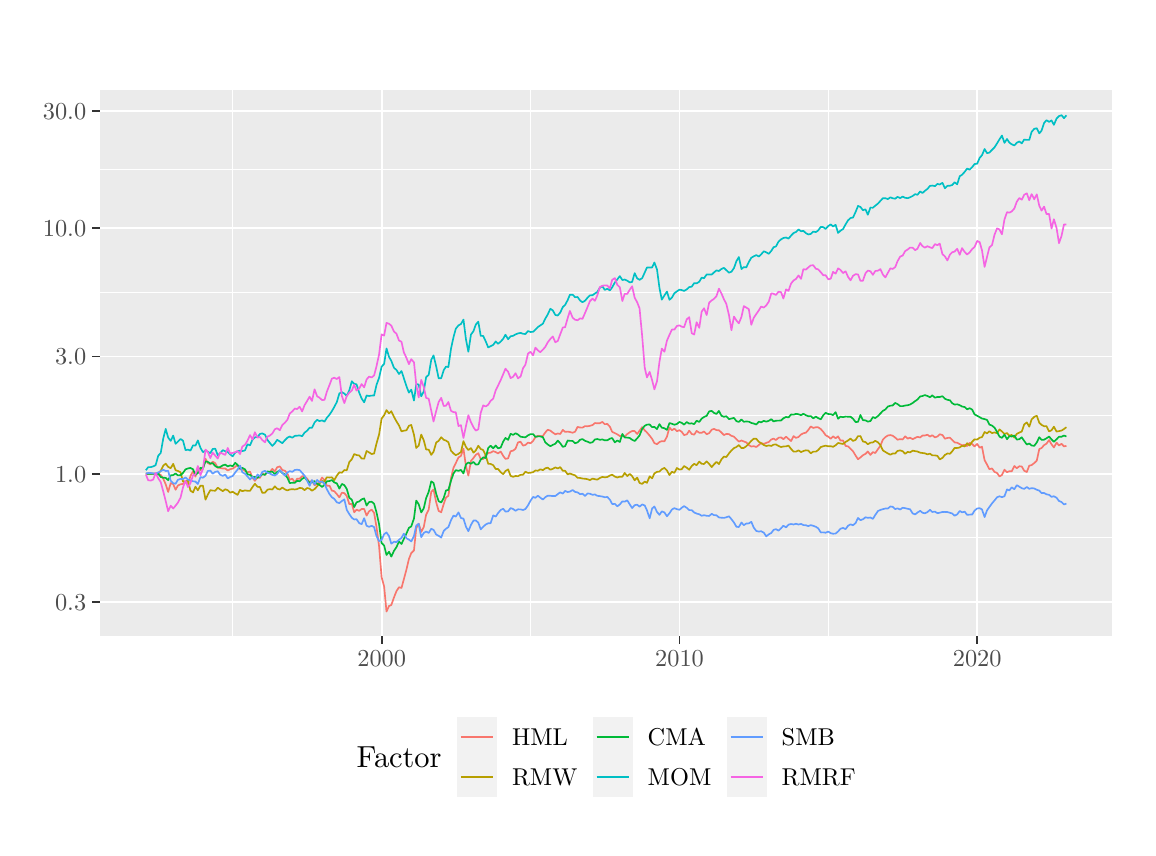
\begin{tikzpicture}[x=1pt,y=1pt]
\definecolor{fillColor}{RGB}{255,255,255}
\path[use as bounding box,fill=fillColor,fill opacity=0.00] (0,0) rectangle (397.48,289.08);
\begin{scope}
\path[clip] (  0.00,  0.00) rectangle (397.48,289.08);
\definecolor{drawColor}{RGB}{255,255,255}
\definecolor{fillColor}{RGB}{255,255,255}

\path[draw=drawColor,line width= 0.6pt,line join=round,line cap=round,fill=fillColor] (  0.00,  0.00) rectangle (397.48,289.08);
\end{scope}
\begin{scope}
\path[clip] ( 26.09, 69.13) rectangle (391.98,266.42);
\definecolor{fillColor}{gray}{0.92}

\path[fill=fillColor] ( 26.09, 69.13) rectangle (391.98,266.42);
\definecolor{drawColor}{RGB}{255,255,255}

\path[draw=drawColor,line width= 0.3pt,line join=round] ( 26.09,104.73) --
	(391.98,104.73);

\path[draw=drawColor,line width= 0.3pt,line join=round] ( 26.09,149.07) --
	(391.98,149.07);

\path[draw=drawColor,line width= 0.3pt,line join=round] ( 26.09,193.40) --
	(391.98,193.40);

\path[draw=drawColor,line width= 0.3pt,line join=round] ( 26.09,237.74) --
	(391.98,237.74);

\path[draw=drawColor,line width= 0.3pt,line join=round] ( 74.11, 69.13) --
	( 74.11,266.42);

\path[draw=drawColor,line width= 0.3pt,line join=round] (181.73, 69.13) --
	(181.73,266.42);

\path[draw=drawColor,line width= 0.3pt,line join=round] (289.33, 69.13) --
	(289.33,266.42);

\path[draw=drawColor,line width= 0.6pt,line join=round] ( 26.09, 81.55) --
	(391.98, 81.55);

\path[draw=drawColor,line width= 0.6pt,line join=round] ( 26.09,127.91) --
	(391.98,127.91);

\path[draw=drawColor,line width= 0.6pt,line join=round] ( 26.09,170.22) --
	(391.98,170.22);

\path[draw=drawColor,line width= 0.6pt,line join=round] ( 26.09,216.58) --
	(391.98,216.58);

\path[draw=drawColor,line width= 0.6pt,line join=round] ( 26.09,258.89) --
	(391.98,258.89);

\path[draw=drawColor,line width= 0.6pt,line join=round] (127.92, 69.13) --
	(127.92,266.42);

\path[draw=drawColor,line width= 0.6pt,line join=round] (235.54, 69.13) --
	(235.54,266.42);

\path[draw=drawColor,line width= 0.6pt,line join=round] (343.12, 69.13) --
	(343.12,266.42);
\definecolor{drawColor}{RGB}{248,118,109}

\path[draw=drawColor,line width= 0.6pt,line join=round] ( 42.72,127.91) --
	( 43.55,127.91) --
	( 44.49,127.91) --
	( 45.37,127.91) --
	( 46.23,127.91) --
	( 47.17,127.91) --
	( 48.08,127.45) --
	( 49.00,126.08) --
	( 49.88,124.07) --
	( 50.76,121.31) --
	( 51.68,124.51) --
	( 52.59,124.14) --
	( 53.45,122.11) --
	( 54.27,123.61) --
	( 55.24,124.08) --
	( 56.13,124.23) --
	( 57.04,125.07) --
	( 57.92,124.27) --
	( 58.81,127.02) --
	( 59.75,128.84) --
	( 60.63,126.84) --
	( 61.49,130.24) --
	( 62.43,129.19) --
	( 63.34,129.73) --
	( 64.26,133.32) --
	( 65.08,131.77) --
	( 66.00,131.26) --
	( 66.85,132.26) --
	( 67.79,131.69) --
	( 68.68,130.06) --
	( 69.53,129.98) --
	( 70.50,129.79) --
	( 71.39,129.79) --
	( 72.30,129.06) --
	( 73.18,129.54) --
	( 74.07,129.73) --
	( 75.01,130.39) --
	( 75.84,131.03) --
	( 76.75,129.52) --
	( 77.57,129.56) --
	( 78.55,128.92) --
	( 79.43,128.43) --
	( 80.34,128.66) --
	( 81.26,126.38) --
	( 82.11,125.35) --
	( 83.05,126.54) --
	( 83.94,126.41) --
	( 84.79,128.05) --
	( 85.76,127.48) --
	( 86.62,128.47) --
	( 87.47,128.51) --
	( 88.41,129.67) --
	( 89.33,128.76) --
	( 90.15,130.23) --
	( 91.12,130.54) --
	( 92.01,129.26) --
	( 92.92,128.98) --
	( 93.84,128.04) --
	( 94.69,125.71) --
	( 95.63,126.13) --
	( 96.55,124.75) --
	( 97.37,126.10) --
	( 98.28,126.09) --
	( 99.17,127.01) --
	(100.05,126.94) --
	(100.96,126.15) --
	(101.88,124.72) --
	(102.73,125.47) --
	(103.67,123.73) --
	(104.59,124.22) --
	(105.41,124.71) --
	(106.38,126.53) --
	(107.27,125.64) --
	(108.09,123.50) --
	(109.04,123.59) --
	(109.92,121.78) --
	(110.77,121.60) --
	(111.72,120.51) --
	(112.63,119.36) --
	(113.54,121.04) --
	(114.43,120.89) --
	(115.31,119.85) --
	(116.22,116.92) --
	(117.14,117.00) --
	(117.99,113.95) --
	(118.82,114.90) --
	(119.79,114.49) --
	(120.67,115.14) --
	(121.59,115.16) --
	(122.47,112.76) --
	(123.35,114.30) --
	(124.30,114.92) --
	(125.18,113.74) --
	(126.03,108.74) --
	(126.98,101.69) --
	(127.89, 90.53) --
	(128.80, 87.16) --
	(129.66, 78.10) --
	(130.57, 80.09) --
	(131.40, 80.47) --
	(132.37, 83.21) --
	(133.25, 85.45) --
	(134.17, 86.88) --
	(135.08, 86.62) --
	(135.93, 89.77) --
	(136.88, 93.33) --
	(137.76, 97.09) --
	(138.61, 99.23) --
	(139.59,100.19) --
	(140.41,108.23) --
	(141.29,109.87) --
	(142.21,106.88) --
	(143.12,108.61) --
	(143.98,113.11) --
	(144.92,114.99) --
	(145.83,121.35) --
	(146.66,122.17) --
	(147.63,117.50) --
	(148.51,114.45) --
	(149.43,113.96) --
	(150.34,116.97) --
	(151.16,119.30) --
	(152.02,119.89) --
	(152.96,126.31) --
	(153.87,130.05) --
	(154.70,131.74) --
	(155.67,133.77) --
	(156.56,134.34) --
	(157.47,136.96) --
	(158.38,130.59) --
	(159.24,127.22) --
	(160.18,132.50) --
	(161.09,133.58) --
	(161.92,134.72) --
	(162.83,135.30) --
	(163.71,133.17) --
	(164.60,133.21) --
	(165.51,134.63) --
	(166.42,135.38) --
	(167.28,135.50) --
	(168.22,136.05) --
	(169.13,135.71) --
	(169.96,135.24) --
	(170.93,135.91) --
	(171.82,134.38) --
	(172.64,133.28) --
	(173.61,133.45) --
	(174.50,136.02) --
	(175.41,136.24) --
	(176.29,136.93) --
	(177.18,139.22) --
	(178.12,139.45) --
	(179.00,138.04) --
	(179.86,138.30) --
	(180.80,139.12) --
	(181.71,138.91) --
	(182.63,139.75) --
	(183.45,141.11) --
	(184.37,141.61) --
	(185.22,141.49) --
	(186.16,141.51) --
	(187.05,142.83) --
	(187.90,143.79) --
	(188.87,143.46) --
	(189.76,142.76) --
	(190.67,142.14) --
	(191.55,142.45) --
	(192.44,142.26) --
	(193.38,143.73) --
	(194.20,143.01) --
	(195.12,143.12) --
	(195.94,142.97) --
	(196.92,142.71) --
	(197.80,143.08) --
	(198.71,144.81) --
	(199.63,144.58) --
	(200.48,144.56) --
	(201.42,145.11) --
	(202.31,145.04) --
	(203.16,145.20) --
	(204.13,145.49) --
	(204.96,146.21) --
	(205.84,146.12) --
	(206.75,146.14) --
	(207.67,146.63) --
	(208.52,145.80) --
	(209.47,145.87) --
	(210.38,144.88) --
	(211.20,143.05) --
	(212.18,142.57) --
	(213.06,142.13) --
	(213.97,141.52) --
	(214.89,141.59) --
	(215.74,141.34) --
	(216.65,142.22) --
	(217.54,142.86) --
	(218.42,143.32) --
	(219.33,143.31) --
	(220.25,142.25) --
	(221.10,143.45) --
	(222.04,144.74) --
	(222.96,143.58) --
	(223.78,142.80) --
	(224.75,141.65) --
	(225.64,140.49) --
	(226.46,138.96) --
	(227.41,138.56) --
	(228.29,139.35) --
	(229.14,139.68) --
	(230.09,139.59) --
	(231.00,141.32) --
	(231.91,144.61) --
	(232.80,143.61) --
	(233.68,144.18) --
	(234.59,143.26) --
	(235.51,143.63) --
	(236.36,143.01) --
	(237.19,141.86) --
	(238.16,142.12) --
	(239.04,143.45) --
	(239.96,142.26) --
	(240.84,142.00) --
	(241.72,143.37) --
	(242.67,142.72) --
	(243.55,142.68) --
	(244.40,143.17) --
	(245.35,142.16) --
	(246.26,142.57) --
	(247.17,143.79) --
	(248.00,144.10) --
	(248.91,143.66) --
	(249.77,143.59) --
	(250.71,142.77) --
	(251.59,141.86) --
	(252.45,142.28) --
	(253.42,142.20) --
	(254.30,141.59) --
	(255.22,141.28) --
	(256.10,140.40) --
	(256.98,139.52) --
	(257.93,139.90) --
	(258.78,139.55) --
	(259.66,139.23) --
	(260.58,138.23) --
	(261.49,137.72) --
	(262.35,137.85) --
	(263.29,137.56) --
	(264.20,138.27) --
	(265.03,138.98) --
	(266.00,138.67) --
	(266.88,139.05) --
	(267.80,139.35) --
	(268.71,140.28) --
	(269.53,140.57) --
	(270.39,140.07) --
	(271.33,140.91) --
	(272.24,141.03) --
	(273.07,140.38) --
	(274.04,141.29) --
	(274.92,140.49) --
	(275.84,139.70) --
	(276.75,141.47) --
	(277.61,140.85) --
	(278.55,141.17) --
	(279.46,142.09) --
	(280.29,142.52) --
	(281.20,142.72) --
	(282.08,143.70) --
	(282.97,144.98) --
	(283.88,144.43) --
	(284.79,144.70) --
	(285.65,144.66) --
	(286.59,144.02) --
	(287.50,143.01) --
	(288.33,141.81) --
	(289.30,141.28) --
	(290.19,140.53) --
	(291.01,141.40) --
	(291.95,140.71) --
	(292.84,141.39) --
	(293.69,139.88) --
	(294.63,139.92) --
	(295.55,137.96) --
	(296.46,137.76) --
	(297.34,136.92) --
	(298.23,136.03) --
	(299.14,134.51) --
	(300.05,133.13) --
	(300.91,133.78) --
	(301.82,134.58) --
	(302.73,135.06) --
	(303.59,135.92) --
	(304.53,134.69) --
	(305.42,135.73) --
	(306.27,135.37) --
	(307.24,136.76) --
	(308.13,138.01) --
	(309.04,140.26) --
	(309.92,141.13) --
	(310.81,141.71) --
	(311.75,141.87) --
	(312.57,141.62) --
	(313.49,140.95) --
	(314.31,140.19) --
	(315.28,140.40) --
	(316.17,140.28) --
	(317.08,141.41) --
	(318.00,140.60) --
	(318.85,140.91) --
	(319.79,140.39) --
	(320.68,140.83) --
	(321.53,141.23) --
	(322.50,140.99) --
	(323.33,141.70) --
	(324.21,141.72) --
	(325.12,141.98) --
	(326.04,141.33) --
	(326.89,141.81) --
	(327.83,141.03) --
	(328.75,141.36) --
	(329.57,142.15) --
	(330.55,141.88) --
	(331.43,140.55) --
	(332.34,140.82) --
	(333.26,140.91) --
	(334.08,140.12) --
	(334.93,139.22) --
	(335.88,139.09) --
	(336.79,138.60) --
	(337.62,138.18) --
	(338.59,138.30) --
	(339.47,137.91) --
	(340.38,139.05) --
	(341.30,138.60) --
	(342.15,137.77) --
	(343.09,138.66) --
	(344.01,137.30) --
	(344.83,137.65) --
	(345.78,132.79) --
	(346.66,131.21) --
	(347.51,129.53) --
	(348.46,129.81) --
	(349.37,128.55) --
	(350.28,128.17) --
	(351.17,126.92) --
	(352.05,127.45) --
	(352.96,129.36) --
	(353.88,128.45) --
	(354.73,128.81) --
	(355.56,128.74) --
	(356.53,130.69) --
	(357.41,129.88) --
	(358.33,130.60) --
	(359.21,130.50) --
	(360.09,128.98) --
	(361.04,128.52) --
	(361.92,130.81) --
	(362.77,131.02) --
	(363.72,131.75) --
	(364.63,132.61) --
	(365.54,136.80) --
	(366.37,137.18) --
	(367.28,138.24) --
	(368.14,138.76) --
	(369.08,140.06) --
	(369.96,138.53) --
	(370.82,137.39) --
	(371.79,139.12) --
	(372.67,138.11) --
	(373.59,138.70) --
	(374.47,137.77) --
	(375.35,137.96);
\definecolor{drawColor}{RGB}{183,159,0}

\path[draw=drawColor,line width= 0.6pt,line join=round] ( 42.72,127.91) --
	( 43.55,127.91) --
	( 44.49,127.91) --
	( 45.37,127.91) --
	( 46.23,127.91) --
	( 47.17,127.91) --
	( 48.08,128.99) --
	( 49.00,130.83) --
	( 49.88,131.54) --
	( 50.76,130.39) --
	( 51.68,129.89) --
	( 52.59,131.46) --
	( 53.45,129.15) --
	( 54.27,128.90) --
	( 55.24,128.43) --
	( 56.13,125.04) --
	( 57.04,125.14) --
	( 57.92,125.52) --
	( 58.81,121.78) --
	( 59.75,121.14) --
	( 60.63,123.21) --
	( 61.49,121.92) --
	( 62.43,123.58) --
	( 63.34,123.54) --
	( 64.26,118.52) --
	( 65.08,120.31) --
	( 66.00,121.97) --
	( 66.85,121.79) --
	( 67.79,121.76) --
	( 68.68,122.84) --
	( 69.53,122.26) --
	( 70.50,121.60) --
	( 71.39,122.28) --
	( 72.30,121.95) --
	( 73.18,121.03) --
	( 74.07,121.40) --
	( 75.01,120.77) --
	( 75.84,120.26) --
	( 76.75,122.05) --
	( 77.57,121.59) --
	( 78.55,121.90) --
	( 79.43,121.72) --
	( 80.34,121.71) --
	( 81.26,123.12) --
	( 82.11,124.27) --
	( 83.05,123.18) --
	( 83.94,123.08) --
	( 84.79,120.99) --
	( 85.76,121.06) --
	( 86.62,122.09) --
	( 87.47,122.35) --
	( 88.41,122.19) --
	( 89.33,123.35) --
	( 90.15,122.48) --
	( 91.12,122.19) --
	( 92.01,122.90) --
	( 92.92,122.25) --
	( 93.84,121.86) --
	( 94.69,122.20) --
	( 95.63,122.32) --
	( 96.55,122.21) --
	( 97.37,122.36) --
	( 98.28,122.77) --
	( 99.17,122.67) --
	(100.05,121.97) --
	(100.96,122.73) --
	(101.88,122.50) --
	(102.73,121.75) --
	(103.67,122.36) --
	(104.59,123.31) --
	(105.41,124.37) --
	(106.38,125.25) --
	(107.27,125.19) --
	(108.09,126.60) --
	(109.04,126.55) --
	(109.92,126.60) --
	(110.77,125.56) --
	(111.72,127.22) --
	(112.63,128.41) --
	(113.54,128.26) --
	(114.43,129.22) --
	(115.31,129.16) --
	(116.22,132.10) --
	(117.14,133.14) --
	(117.99,135.02) --
	(118.82,134.65) --
	(119.79,134.50) --
	(120.67,133.39) --
	(121.59,133.33) --
	(122.47,136.11) --
	(123.35,135.61) --
	(124.30,135.01) --
	(125.18,135.23) --
	(126.03,138.75) --
	(126.98,142.09) --
	(127.89,147.82) --
	(128.80,149.02) --
	(129.66,150.89) --
	(130.57,149.69) --
	(131.40,150.48) --
	(132.37,148.43) --
	(133.25,146.83) --
	(134.17,145.34) --
	(135.08,143.20) --
	(135.93,143.44) --
	(136.88,143.60) --
	(137.76,145.21) --
	(138.61,145.52) --
	(139.59,141.96) --
	(140.41,137.19) --
	(141.29,138.04) --
	(142.21,142.05) --
	(143.12,139.98) --
	(143.98,136.68) --
	(144.92,136.58) --
	(145.83,134.70) --
	(146.66,135.85) --
	(147.63,139.18) --
	(148.51,139.79) --
	(149.43,141.08) --
	(150.34,140.15) --
	(151.16,139.86) --
	(152.02,139.28) --
	(152.96,136.22) --
	(153.87,135.24) --
	(154.70,134.61) --
	(155.67,135.08) --
	(156.56,135.77) --
	(157.47,139.65) --
	(158.38,137.56) --
	(159.24,136.45) --
	(160.18,137.16) --
	(161.09,135.52) --
	(161.92,136.31) --
	(162.83,138.00) --
	(163.71,136.85) --
	(164.60,136.43) --
	(165.51,134.54) --
	(166.42,131.45) --
	(167.28,131.45) --
	(168.22,130.99) --
	(169.13,129.59) --
	(169.96,129.62) --
	(170.93,128.45) --
	(171.82,127.74) --
	(172.64,128.86) --
	(173.61,129.47) --
	(174.50,127.13) --
	(175.41,126.79) --
	(176.29,127.07) --
	(177.18,127.01) --
	(178.12,127.49) --
	(179.00,127.55) --
	(179.86,128.63) --
	(180.80,128.18) --
	(181.71,128.28) --
	(182.63,128.45) --
	(183.45,129.07) --
	(184.37,128.97) --
	(185.22,129.50) --
	(186.16,129.19) --
	(187.05,129.86) --
	(187.90,130.09) --
	(188.87,129.35) --
	(189.76,129.67) --
	(190.67,130.19) --
	(191.55,129.79) --
	(192.44,130.28) --
	(193.38,128.94) --
	(194.20,128.96) --
	(195.12,127.66) --
	(195.94,127.97) --
	(196.92,127.60) --
	(197.80,127.31) --
	(198.71,126.42) --
	(199.63,126.37) --
	(200.48,126.15) --
	(201.42,126.08) --
	(202.31,125.92) --
	(203.16,125.59) --
	(204.13,126.14) --
	(204.96,125.92) --
	(205.84,125.75) --
	(206.75,126.35) --
	(207.67,126.75) --
	(208.52,126.60) --
	(209.47,126.71) --
	(210.38,127.25) --
	(211.20,127.54) --
	(212.18,126.86) --
	(213.06,126.54) --
	(213.97,126.83) --
	(214.89,126.82) --
	(215.74,128.18) --
	(216.65,127.05) --
	(217.54,127.84) --
	(218.42,127.03) --
	(219.33,125.52) --
	(220.25,126.49) --
	(221.10,124.58) --
	(222.04,124.22) --
	(222.96,125.07) --
	(223.78,124.63) --
	(224.75,126.96) --
	(225.64,126.23) --
	(226.46,128.01) --
	(227.41,128.57) --
	(228.29,128.69) --
	(229.14,129.52) --
	(230.09,130.02) --
	(231.00,129.06) --
	(231.91,127.41) --
	(232.80,128.60) --
	(233.68,128.21) --
	(234.59,129.97) --
	(235.51,129.39) --
	(236.36,129.55) --
	(237.19,130.67) --
	(238.16,130.07) --
	(239.04,129.34) --
	(239.96,130.68) --
	(240.84,131.47) --
	(241.72,130.98) --
	(242.67,132.28) --
	(243.55,131.50) --
	(244.40,131.40) --
	(245.35,132.35) --
	(246.26,131.42) --
	(247.17,130.29) --
	(248.00,131.29) --
	(248.91,132.17) --
	(249.77,131.38) --
	(250.71,133.10) --
	(251.59,134.10) --
	(252.45,133.92) --
	(253.42,135.26) --
	(254.30,136.30) --
	(255.22,137.14) --
	(256.10,137.56) --
	(256.98,138.25) --
	(257.93,137.14) --
	(258.78,137.22) --
	(259.66,137.82) --
	(260.58,138.77) --
	(261.49,139.79) --
	(262.35,140.54) --
	(263.29,140.52) --
	(264.20,139.42) --
	(265.03,138.95) --
	(266.00,138.27) --
	(266.88,137.92) --
	(267.80,138.12) --
	(268.71,137.93) --
	(269.53,138.41) --
	(270.39,138.46) --
	(271.33,137.94) --
	(272.24,137.53) --
	(273.07,137.75) --
	(274.04,137.79) --
	(274.92,138.06) --
	(275.84,136.86) --
	(276.75,135.91) --
	(277.61,135.88) --
	(278.55,136.34) --
	(279.46,135.71) --
	(280.29,136.10) --
	(281.20,136.36) --
	(282.08,136.27) --
	(282.97,135.27) --
	(283.88,135.89) --
	(284.79,135.87) --
	(285.65,136.46) --
	(286.59,137.53) --
	(287.50,137.83) --
	(288.33,138.03) --
	(289.30,137.81) --
	(290.19,137.86) --
	(291.01,137.62) --
	(291.95,138.18) --
	(292.84,139.00) --
	(293.69,138.83) --
	(294.63,138.65) --
	(295.55,139.38) --
	(296.46,139.92) --
	(297.34,140.63) --
	(298.23,139.75) --
	(299.14,140.11) --
	(300.05,141.49) --
	(300.91,141.50) --
	(301.82,139.54) --
	(302.73,139.34) --
	(303.59,138.54) --
	(304.53,139.11) --
	(305.42,139.21) --
	(306.27,139.79) --
	(307.24,139.24) --
	(308.13,138.24) --
	(309.04,136.30) --
	(309.92,135.77) --
	(310.81,135.23) --
	(311.75,134.75) --
	(312.57,135.21) --
	(313.49,135.20) --
	(314.31,136.15) --
	(315.28,136.32) --
	(316.17,136.04) --
	(317.08,135.09) --
	(318.00,135.78) --
	(318.85,135.62) --
	(319.79,136.23) --
	(320.68,136.06) --
	(321.53,135.92) --
	(322.50,135.50) --
	(323.33,135.39) --
	(324.21,135.27) --
	(325.12,134.89) --
	(326.04,135.14) --
	(326.89,134.52) --
	(327.83,134.52) --
	(328.75,134.36) --
	(329.57,133.08) --
	(330.55,133.61) --
	(331.43,134.67) --
	(332.34,135.21) --
	(333.26,135.11) --
	(334.08,135.99) --
	(334.93,137.21) --
	(335.88,137.21) --
	(336.79,137.38) --
	(337.62,138.02) --
	(338.59,137.75) --
	(339.47,138.92) --
	(340.38,138.11) --
	(341.30,139.49) --
	(342.15,140.33) --
	(343.09,140.24) --
	(344.01,140.92) --
	(344.83,141.10) --
	(345.78,142.97) --
	(346.66,142.48) --
	(347.51,143.25) --
	(348.46,142.58) --
	(349.37,142.82) --
	(350.28,142.54) --
	(351.17,143.89) --
	(352.05,143.19) --
	(352.96,142.26) --
	(353.88,142.59) --
	(354.73,141.61) --
	(355.56,141.91) --
	(356.53,140.93) --
	(357.41,142.29) --
	(358.33,142.77) --
	(359.21,143.14) --
	(360.09,145.71) --
	(361.04,146.43) --
	(361.92,144.89) --
	(362.77,147.51) --
	(363.72,148.45) --
	(364.63,148.84) --
	(365.54,146.32) --
	(366.37,145.54) --
	(367.28,145.05) --
	(368.14,145.11) --
	(369.08,143.21) --
	(369.96,143.58) --
	(370.82,144.89) --
	(371.79,143.13) --
	(372.67,143.30) --
	(373.59,143.50) --
	(374.47,144.05) --
	(375.35,144.72);
\definecolor{drawColor}{RGB}{0,186,56}

\path[draw=drawColor,line width= 0.6pt,line join=round] ( 42.72,127.91) --
	( 43.55,127.91) --
	( 44.49,127.91) --
	( 45.37,127.91) --
	( 46.23,127.91) --
	( 47.17,127.91) --
	( 48.08,126.72) --
	( 49.00,126.45) --
	( 49.88,126.40) --
	( 50.76,125.56) --
	( 51.68,127.31) --
	( 52.59,127.40) --
	( 53.45,127.98) --
	( 54.27,127.31) --
	( 55.24,127.33) --
	( 56.13,128.21) --
	( 57.04,129.48) --
	( 57.92,129.81) --
	( 58.81,129.98) --
	( 59.75,129.51) --
	( 60.63,127.54) --
	( 61.49,128.12) --
	( 62.43,130.04) --
	( 63.34,129.82) --
	( 64.26,132.38) --
	( 65.08,132.17) --
	( 66.00,131.60) --
	( 66.85,131.73) --
	( 67.79,130.65) --
	( 68.68,130.18) --
	( 69.53,130.33) --
	( 70.50,130.92) --
	( 71.39,131.20) --
	( 72.30,130.55) --
	( 73.18,130.90) --
	( 74.07,130.60) --
	( 75.01,131.84) --
	( 75.84,131.09) --
	( 76.75,129.76) --
	( 77.57,130.00) --
	( 78.55,129.47) --
	( 79.43,127.70) --
	( 80.34,127.48) --
	( 81.26,126.69) --
	( 82.11,126.75) --
	( 83.05,126.44) --
	( 83.94,127.06) --
	( 84.79,127.68) --
	( 85.76,127.51) --
	( 86.62,128.74) --
	( 87.47,128.53) --
	( 88.41,128.69) --
	( 89.33,127.75) --
	( 90.15,128.53) --
	( 91.12,129.05) --
	( 92.01,128.17) --
	( 92.92,127.65) --
	( 93.84,126.45) --
	( 94.69,124.54) --
	( 95.63,124.62) --
	( 96.55,124.64) --
	( 97.37,125.34) --
	( 98.28,125.17) --
	( 99.17,126.04) --
	(100.05,126.62) --
	(100.96,125.52) --
	(101.88,124.66) --
	(102.73,124.76) --
	(103.67,125.22) --
	(104.59,124.29) --
	(105.41,123.88) --
	(106.38,123.13) --
	(107.27,123.88) --
	(108.09,125.15) --
	(109.04,125.26) --
	(109.92,125.60) --
	(110.77,124.78) --
	(111.72,124.40) --
	(112.63,122.50) --
	(113.54,124.19) --
	(114.43,123.77) --
	(115.31,122.38) --
	(116.22,119.20) --
	(117.14,118.50) --
	(117.99,115.84) --
	(118.82,117.55) --
	(119.79,117.87) --
	(120.67,118.64) --
	(121.59,118.97) --
	(122.47,116.39) --
	(123.35,117.65) --
	(124.30,117.79) --
	(125.18,117.05) --
	(126.03,114.00) --
	(126.98,109.61) --
	(127.89,102.88) --
	(128.80,101.94) --
	(129.66, 98.55) --
	(130.57, 99.69) --
	(131.40, 97.95) --
	(132.37,100.05) --
	(133.25,101.36) --
	(134.17,103.38) --
	(135.08,102.51) --
	(135.93,104.33) --
	(136.88,106.34) --
	(137.76,108.34) --
	(138.61,108.87) --
	(139.59,111.72) --
	(140.41,118.18) --
	(141.29,116.86) --
	(142.21,113.91) --
	(143.12,115.38) --
	(143.98,119.07) --
	(144.92,121.39) --
	(145.83,125.13) --
	(146.66,124.57) --
	(147.63,120.61) --
	(148.51,117.97) --
	(149.43,117.50) --
	(150.34,119.13) --
	(151.16,121.87) --
	(152.02,122.05) --
	(152.96,125.33) --
	(153.87,127.97) --
	(154.70,129.20) --
	(155.67,128.92) --
	(156.56,129.29) --
	(157.47,127.99) --
	(158.38,131.29) --
	(159.24,131.96) --
	(160.18,131.49) --
	(161.09,132.17) --
	(161.92,131.21) --
	(162.83,131.28) --
	(163.71,133.01) --
	(164.60,133.78) --
	(165.51,133.56) --
	(166.42,137.20) --
	(167.28,138.01) --
	(168.22,137.09) --
	(169.13,138.08) --
	(169.96,137.07) --
	(170.93,137.37) --
	(171.82,139.50) --
	(172.64,140.82) --
	(173.61,140.14) --
	(174.50,142.33) --
	(175.41,141.92) --
	(176.29,142.53) --
	(177.18,142.05) --
	(178.12,141.26) --
	(179.00,141.14) --
	(179.86,141.05) --
	(180.80,141.77) --
	(181.71,142.22) --
	(182.63,142.22) --
	(183.45,141.23) --
	(184.37,141.38) --
	(185.22,141.38) --
	(186.16,141.12) --
	(187.05,139.23) --
	(187.90,138.50) --
	(188.87,137.82) --
	(189.76,138.33) --
	(190.67,138.74) --
	(191.55,139.87) --
	(192.44,138.92) --
	(193.38,137.60) --
	(194.20,137.88) --
	(195.12,139.89) --
	(195.94,139.78) --
	(196.92,139.74) --
	(197.80,138.91) --
	(198.71,139.21) --
	(199.63,140.19) --
	(200.48,140.41) --
	(201.42,139.77) --
	(202.31,139.48) --
	(203.16,139.05) --
	(204.13,139.28) --
	(204.96,140.28) --
	(205.84,140.44) --
	(206.75,140.16) --
	(207.67,140.28) --
	(208.52,139.97) --
	(209.47,140.00) --
	(210.38,140.55) --
	(211.20,140.80) --
	(212.18,139.23) --
	(213.06,139.92) --
	(213.97,139.36) --
	(214.89,142.27) --
	(215.74,140.98) --
	(216.65,140.95) --
	(217.54,140.82) --
	(218.42,140.17) --
	(219.33,139.72) --
	(220.25,140.69) --
	(221.10,141.73) --
	(222.04,144.08) --
	(222.96,145.20) --
	(223.78,145.64) --
	(224.75,145.69) --
	(225.64,144.72) --
	(226.46,144.82) --
	(227.41,144.02) --
	(228.29,145.82) --
	(229.14,144.54) --
	(230.09,144.33) --
	(231.00,143.75) --
	(231.91,146.21) --
	(232.80,145.94) --
	(233.68,145.60) --
	(234.59,145.88) --
	(235.51,146.60) --
	(236.36,146.27) --
	(237.19,145.64) --
	(238.16,146.57) --
	(239.04,145.99) --
	(239.96,146.12) --
	(240.84,145.82) --
	(241.72,147.05) --
	(242.67,146.61) --
	(243.55,147.82) --
	(244.40,148.40) --
	(245.35,148.83) --
	(246.26,150.43) --
	(247.17,150.59) --
	(248.00,149.87) --
	(248.91,149.51) --
	(249.77,150.58) --
	(250.71,148.83) --
	(251.59,148.47) --
	(252.45,148.67) --
	(253.42,147.63) --
	(254.30,147.84) --
	(255.22,148.06) --
	(256.10,146.91) --
	(256.98,146.61) --
	(257.93,147.51) --
	(258.78,146.67) --
	(259.66,146.78) --
	(260.58,146.70) --
	(261.49,146.24) --
	(262.35,146.04) --
	(263.29,145.69) --
	(264.20,146.70) --
	(265.03,146.47) --
	(266.00,147.00) --
	(266.88,146.70) --
	(267.80,147.02) --
	(268.71,147.61) --
	(269.53,146.80) --
	(270.39,147.06) --
	(271.33,147.08) --
	(272.24,147.14) --
	(273.07,147.93) --
	(274.04,148.40) --
	(274.92,148.24) --
	(275.84,149.30) --
	(276.75,149.24) --
	(277.61,149.54) --
	(278.55,149.40) --
	(279.46,149.05) --
	(280.29,149.57) --
	(281.20,149.05) --
	(282.08,148.67) --
	(282.97,148.72) --
	(283.88,147.92) --
	(284.79,148.53) --
	(285.65,147.98) --
	(286.59,147.57) --
	(287.50,149.04) --
	(288.33,149.91) --
	(289.30,149.46) --
	(290.19,149.43) --
	(291.01,149.08) --
	(291.95,150.14) --
	(292.84,147.75) --
	(293.69,148.52) --
	(294.63,148.33) --
	(295.55,148.55) --
	(296.46,148.49) --
	(297.34,148.49) --
	(298.23,147.78) --
	(299.14,146.61) --
	(300.05,146.62) --
	(300.91,149.13) --
	(301.82,147.27) --
	(302.73,147.18) --
	(303.59,146.72) --
	(304.53,146.93) --
	(305.42,148.36) --
	(306.27,148.01) --
	(307.24,148.74) --
	(308.13,149.66) --
	(309.04,150.64) --
	(309.92,151.11) --
	(310.81,152.16) --
	(311.75,152.49) --
	(312.57,152.57) --
	(313.49,153.48) --
	(314.31,153.07) --
	(315.28,152.33) --
	(316.17,152.31) --
	(317.08,152.54) --
	(318.00,152.66) --
	(318.85,152.90) --
	(319.79,153.46) --
	(320.68,154.14) --
	(321.53,154.72) --
	(322.50,155.83) --
	(323.33,155.97) --
	(324.21,156.33) --
	(325.12,155.98) --
	(326.04,155.52) --
	(326.89,156.22) --
	(327.83,155.38) --
	(328.75,155.64) --
	(329.57,155.63) --
	(330.55,155.90) --
	(331.43,155.00) --
	(332.34,154.59) --
	(333.26,154.45) --
	(334.08,153.36) --
	(334.93,152.90) --
	(335.88,152.98) --
	(336.79,152.66) --
	(337.62,152.19) --
	(338.59,151.99) --
	(339.47,151.18) --
	(340.38,151.56) --
	(341.30,151.08) --
	(342.15,149.34) --
	(343.09,148.83) --
	(344.01,148.33) --
	(344.83,147.85) --
	(345.78,147.64) --
	(346.66,147.34) --
	(347.51,145.64) --
	(348.46,145.30) --
	(349.37,144.54) --
	(350.28,143.05) --
	(351.17,141.29) --
	(352.05,140.86) --
	(352.96,142.03) --
	(353.88,140.37) --
	(354.73,141.47) --
	(355.56,141.35) --
	(356.53,141.70) --
	(357.41,140.24) --
	(358.33,140.38) --
	(359.21,141.06) --
	(360.09,139.75) --
	(361.04,138.45) --
	(361.92,138.83) --
	(362.77,138.10) --
	(363.72,137.96) --
	(364.63,139.20) --
	(365.54,141.09) --
	(366.37,140.12) --
	(367.28,140.20) --
	(368.14,140.70) --
	(369.08,141.33) --
	(369.96,140.30) --
	(370.82,139.45) --
	(371.79,140.35) --
	(372.67,141.26) --
	(373.59,141.27) --
	(374.47,141.70) --
	(375.35,141.34);
\definecolor{drawColor}{RGB}{0,191,196}

\path[draw=drawColor,line width= 0.6pt,line join=round] ( 42.72,129.15) --
	( 43.55,130.28) --
	( 44.49,130.29) --
	( 45.37,130.57) --
	( 46.23,130.96) --
	( 47.17,134.39) --
	( 48.08,135.42) --
	( 49.00,140.66) --
	( 49.88,144.10) --
	( 50.76,140.96) --
	( 51.68,139.78) --
	( 52.59,141.67) --
	( 53.45,138.71) --
	( 54.27,139.48) --
	( 55.24,140.46) --
	( 56.13,139.84) --
	( 57.04,136.42) --
	( 57.92,136.60) --
	( 58.81,136.26) --
	( 59.75,138.16) --
	( 60.63,138.06) --
	( 61.49,139.93) --
	( 62.43,137.25) --
	( 63.34,135.71) --
	( 64.26,136.21) --
	( 65.08,135.84) --
	( 66.00,135.32) --
	( 66.85,136.83) --
	( 67.79,136.96) --
	( 68.68,134.58) --
	( 69.53,135.25) --
	( 70.50,136.42) --
	( 71.39,136.02) --
	( 72.30,135.76) --
	( 73.18,134.89) --
	( 74.07,134.17) --
	( 75.01,135.57) --
	( 75.84,136.00) --
	( 76.75,136.26) --
	( 77.57,136.07) --
	( 78.55,136.34) --
	( 79.43,138.53) --
	( 80.34,138.14) --
	( 81.26,140.26) --
	( 82.11,141.03) --
	( 83.05,141.18) --
	( 83.94,142.28) --
	( 84.79,142.46) --
	( 85.76,142.01) --
	( 86.62,140.13) --
	( 87.47,139.07) --
	( 88.41,137.94) --
	( 89.33,138.92) --
	( 90.15,140.15) --
	( 91.12,139.53) --
	( 92.01,138.93) --
	( 92.92,139.99) --
	( 93.84,140.90) --
	( 94.69,141.35) --
	( 95.63,140.92) --
	( 96.55,141.58) --
	( 97.37,141.64) --
	( 98.28,141.74) --
	( 99.17,141.44) --
	(100.05,142.74) --
	(100.96,143.43) --
	(101.88,144.52) --
	(102.73,144.47) --
	(103.67,146.42) --
	(104.59,147.38) --
	(105.41,146.92) --
	(106.38,147.16) --
	(107.27,146.73) --
	(108.09,148.09) --
	(109.04,149.19) --
	(109.92,150.52) --
	(110.77,151.98) --
	(111.72,153.82) --
	(112.63,156.92) --
	(113.54,157.35) --
	(114.43,156.86) --
	(115.31,156.03) --
	(116.22,158.05) --
	(117.14,161.31) --
	(117.99,160.36) --
	(118.82,160.22) --
	(119.79,157.23) --
	(120.67,155.08) --
	(121.59,153.69) --
	(122.47,156.17) --
	(123.35,155.99) --
	(124.30,156.13) --
	(125.18,156.15) --
	(126.03,159.93) --
	(126.98,162.56) --
	(127.89,166.58) --
	(128.80,167.57) --
	(129.66,173.16) --
	(130.57,170.12) --
	(131.40,168.67) --
	(132.37,166.16) --
	(133.25,165.41) --
	(134.17,163.93) --
	(135.08,165.00) --
	(135.93,162.42) --
	(136.88,159.49) --
	(137.76,157.19) --
	(138.61,158.29) --
	(139.59,154.33) --
	(140.41,160.28) --
	(141.29,160.14) --
	(142.21,155.86) --
	(143.12,157.63) --
	(143.98,162.79) --
	(144.92,163.65) --
	(145.83,169.05) --
	(146.66,170.65) --
	(147.63,166.58) --
	(148.51,162.36) --
	(149.43,162.41) --
	(150.34,165.33) --
	(151.16,166.61) --
	(152.02,166.45) --
	(152.96,173.04) --
	(153.87,177.24) --
	(154.70,180.29) --
	(155.67,181.51) --
	(156.56,181.98) --
	(157.47,183.59) --
	(158.38,176.39) --
	(159.24,171.98) --
	(160.18,178.17) --
	(161.09,179.43) --
	(161.92,181.77) --
	(162.83,182.85) --
	(163.71,177.72) --
	(164.60,177.68) --
	(165.51,175.74) --
	(166.42,173.52) --
	(167.28,173.97) --
	(168.22,174.45) --
	(169.13,175.70) --
	(169.96,174.82) --
	(170.93,175.65) --
	(171.82,176.65) --
	(172.64,178.12) --
	(173.61,176.49) --
	(174.50,177.56) --
	(175.41,177.72) --
	(176.29,178.25) --
	(177.18,178.60) --
	(178.12,178.79) --
	(179.00,178.46) --
	(179.86,178.38) --
	(180.80,179.46) --
	(181.71,179.11) --
	(182.63,179.19) --
	(183.45,179.93) --
	(184.37,180.90) --
	(185.22,181.46) --
	(186.16,182.10) --
	(187.05,183.95) --
	(187.90,185.41) --
	(188.87,187.50) --
	(189.76,186.90) --
	(190.67,185.26) --
	(191.55,185.07) --
	(192.44,186.14) --
	(193.38,188.16) --
	(194.20,188.87) --
	(195.12,190.63) --
	(195.94,192.57) --
	(196.92,192.60) --
	(197.80,191.69) --
	(198.71,191.74) --
	(199.63,190.47) --
	(200.48,189.87) --
	(201.42,190.42) --
	(202.31,191.51) --
	(203.16,192.34) --
	(204.13,192.42) --
	(204.96,193.01) --
	(205.84,193.57) --
	(206.75,195.11) --
	(207.67,195.66) --
	(208.52,194.32) --
	(209.47,194.75) --
	(210.38,194.15) --
	(211.20,195.25) --
	(212.18,197.01) --
	(213.06,198.10) --
	(213.97,199.31) --
	(214.89,197.88) --
	(215.74,198.07) --
	(216.65,197.66) --
	(217.54,197.04) --
	(218.42,197.21) --
	(219.33,200.38) --
	(220.25,198.49) --
	(221.10,197.97) --
	(222.04,198.55) --
	(222.96,200.59) --
	(223.78,202.42) --
	(224.75,202.43) --
	(225.64,202.44) --
	(226.46,204.23) --
	(227.41,201.68) --
	(228.29,195.06) --
	(229.14,190.82) --
	(230.09,192.32) --
	(231.00,193.72) --
	(231.91,190.75) --
	(232.80,191.55) --
	(233.68,193.11) --
	(234.59,193.79) --
	(235.51,194.41) --
	(236.36,194.25) --
	(237.19,193.95) --
	(238.16,194.51) --
	(239.04,195.33) --
	(239.96,195.50) --
	(240.84,196.78) --
	(241.72,196.68) --
	(242.67,197.27) --
	(243.55,198.76) --
	(244.40,198.53) --
	(245.35,199.92) --
	(246.26,199.88) --
	(247.17,199.85) --
	(248.00,200.64) --
	(248.91,201.38) --
	(249.77,201.14) --
	(250.71,201.90) --
	(251.59,202.28) --
	(252.45,201.46) --
	(253.42,200.54) --
	(254.30,200.89) --
	(255.22,202.21) --
	(256.10,204.70) --
	(256.98,206.19) --
	(257.93,201.86) --
	(258.78,202.57) --
	(259.66,202.44) --
	(260.58,204.41) --
	(261.49,205.95) --
	(262.35,206.46) --
	(263.29,206.89) --
	(264.20,206.38) --
	(265.03,207.16) --
	(266.00,208.27) --
	(266.88,207.91) --
	(267.80,207.35) --
	(268.71,208.44) --
	(269.53,209.74) --
	(270.39,210.04) --
	(271.33,211.79) --
	(272.24,212.59) --
	(273.07,213.08) --
	(274.04,213.25) --
	(274.92,212.85) --
	(275.84,213.93) --
	(276.75,214.86) --
	(277.61,215.25) --
	(278.55,216.18) --
	(279.46,215.51) --
	(280.29,215.67) --
	(281.20,214.84) --
	(282.08,214.36) --
	(282.97,214.55) --
	(283.88,215.40) --
	(284.79,215.20) --
	(285.65,215.81) --
	(286.59,217.09) --
	(287.50,217.00) --
	(288.33,216.34) --
	(289.30,217.42) --
	(290.19,217.98) --
	(291.01,217.24) --
	(291.95,217.84) --
	(292.84,214.90) --
	(293.69,215.72) --
	(294.63,216.30) --
	(295.55,218.01) --
	(296.46,219.48) --
	(297.34,220.30) --
	(298.23,220.48) --
	(299.14,222.42) --
	(300.05,224.66) --
	(300.91,224.30) --
	(301.82,223.10) --
	(302.73,223.44) --
	(303.59,221.49) --
	(304.53,224.07) --
	(305.42,224.02) --
	(306.27,224.74) --
	(307.24,225.50) --
	(308.13,226.49) --
	(309.04,227.46) --
	(309.92,227.47) --
	(310.81,227.14) --
	(311.75,227.77) --
	(312.57,227.44) --
	(313.49,227.27) --
	(314.31,227.94) --
	(315.28,227.50) --
	(316.17,228.04) --
	(317.08,227.60) --
	(318.00,227.46) --
	(318.85,227.79) --
	(319.79,228.26) --
	(320.68,228.92) --
	(321.53,228.69) --
	(322.50,229.91) --
	(323.33,229.32) --
	(324.21,230.12) --
	(325.12,230.80) --
	(326.04,231.91) --
	(326.89,232.02) --
	(327.83,231.81) --
	(328.75,232.62) --
	(329.57,232.40) --
	(330.55,233.02) --
	(331.43,231.06) --
	(332.34,231.92) --
	(333.26,231.98) --
	(334.08,232.22) --
	(334.93,233.21) --
	(335.88,232.49) --
	(336.79,235.40) --
	(337.62,235.91) --
	(338.59,236.99) --
	(339.47,238.17) --
	(340.38,237.78) --
	(341.30,238.69) --
	(342.15,239.80) --
	(343.09,239.92) --
	(344.01,242.06) --
	(344.83,242.97) --
	(345.78,245.23) --
	(346.66,243.73) --
	(347.51,243.93) --
	(348.46,244.94) --
	(349.37,245.83) --
	(350.28,247.27) --
	(351.17,248.75) --
	(352.05,250.09) --
	(352.96,247.44) --
	(353.88,248.83) --
	(354.73,247.53) --
	(355.56,246.96) --
	(356.53,246.51) --
	(357.41,247.49) --
	(358.33,247.96) --
	(359.21,247.27) --
	(360.09,248.65) --
	(361.04,248.53) --
	(361.92,248.52) --
	(362.77,251.42) --
	(363.72,252.52) --
	(364.63,252.74) --
	(365.54,250.88) --
	(366.37,251.88) --
	(367.28,254.63) --
	(368.14,255.65) --
	(369.08,255.04) --
	(369.96,255.55) --
	(370.82,253.97) --
	(371.79,256.24) --
	(372.67,257.12) --
	(373.59,257.45) --
	(374.47,256.38) --
	(375.35,257.41);
\definecolor{drawColor}{RGB}{97,156,255}

\path[draw=drawColor,line width= 0.6pt,line join=round] ( 42.72,127.93) --
	( 43.55,128.19) --
	( 44.49,128.16) --
	( 45.37,127.99) --
	( 46.23,127.91) --
	( 47.17,128.36) --
	( 48.08,128.81) --
	( 49.00,129.34) --
	( 49.88,128.89) --
	( 50.76,128.95) --
	( 51.68,125.37) --
	( 52.59,124.46) --
	( 53.45,124.28) --
	( 54.27,125.69) --
	( 55.24,126.03) --
	( 56.13,125.98) --
	( 57.04,126.56) --
	( 57.92,125.75) --
	( 58.81,125.52) --
	( 59.75,125.16) --
	( 60.63,125.07) --
	( 61.49,124.17) --
	( 62.43,126.68) --
	( 63.34,126.46) --
	( 64.26,127.17) --
	( 65.08,128.88) --
	( 66.00,129.04) --
	( 66.85,127.91) --
	( 67.79,128.57) --
	( 68.68,128.78) --
	( 69.53,127.57) --
	( 70.50,127.10) --
	( 71.39,127.60) --
	( 72.30,126.19) --
	( 73.18,126.73) --
	( 74.07,127.04) --
	( 75.01,128.37) --
	( 75.84,129.39) --
	( 76.75,130.84) --
	( 77.57,128.42) --
	( 78.55,127.87) --
	( 79.43,126.94) --
	( 80.34,125.82) --
	( 81.26,126.80) --
	( 82.11,125.81) --
	( 83.05,127.64) --
	( 83.94,126.93) --
	( 84.79,128.55) --
	( 85.76,128.96) --
	( 86.62,128.25) --
	( 87.47,127.99) --
	( 88.41,127.48) --
	( 89.33,127.25) --
	( 90.15,127.83) --
	( 91.12,129.24) --
	( 92.01,128.22) --
	( 92.92,127.20) --
	( 93.84,128.33) --
	( 94.69,128.83) --
	( 95.63,128.59) --
	( 96.55,129.26) --
	( 97.37,129.34) --
	( 98.28,129.21) --
	( 99.17,128.19) --
	(100.05,127.21) --
	(100.96,125.44) --
	(101.88,123.50) --
	(102.73,125.60) --
	(103.67,124.05) --
	(104.59,125.65) --
	(105.41,124.84) --
	(106.38,125.10) --
	(107.27,124.24) --
	(108.09,122.32) --
	(109.04,120.57) --
	(109.92,119.38) --
	(110.77,118.85) --
	(111.72,117.55) --
	(112.63,117.29) --
	(113.54,118.04) --
	(114.43,118.62) --
	(115.31,114.82) --
	(116.22,113.31) --
	(117.14,111.97) --
	(117.99,111.37) --
	(118.82,111.47) --
	(119.79,110.06) --
	(120.67,109.65) --
	(121.59,111.84) --
	(122.47,109.09) --
	(123.35,108.72) --
	(124.30,109.07) --
	(125.18,108.62) --
	(126.03,105.38) --
	(126.98,103.54) --
	(127.89,103.95) --
	(128.80,106.04) --
	(129.66,106.68) --
	(130.57,105.35) --
	(131.40,102.61) --
	(132.37,103.31) --
	(133.25,103.19) --
	(134.17,104.01) --
	(135.08,104.73) --
	(135.93,106.24) --
	(136.88,104.57) --
	(137.76,104.10) --
	(138.61,103.43) --
	(139.59,105.41) --
	(140.41,109.18) --
	(141.29,109.81) --
	(142.21,104.96) --
	(143.12,106.49) --
	(143.98,107.00) --
	(144.92,106.50) --
	(145.83,108.02) --
	(146.66,107.62) --
	(147.63,105.92) --
	(148.51,105.46) --
	(149.43,104.84) --
	(150.34,107.25) --
	(151.16,108.03) --
	(152.02,108.60) --
	(152.96,111.08) --
	(153.87,112.79) --
	(154.70,112.41) --
	(155.67,113.93) --
	(156.56,111.89) --
	(157.47,111.67) --
	(158.38,108.77) --
	(159.24,107.13) --
	(160.18,109.41) --
	(161.09,110.97) --
	(161.92,111.02) --
	(162.83,110.23) --
	(163.71,107.79) --
	(164.60,108.74) --
	(165.51,109.54) --
	(166.42,110.01) --
	(167.28,110.02) --
	(168.22,112.85) --
	(169.13,112.43) --
	(169.96,113.65) --
	(170.93,114.81) --
	(171.82,115.25) --
	(172.64,114.22) --
	(173.61,114.30) --
	(174.50,115.48) --
	(175.41,115.15) --
	(176.29,114.50) --
	(177.18,115.04) --
	(178.12,115.00) --
	(179.00,114.78) --
	(179.86,115.15) --
	(180.80,116.48) --
	(181.71,118.16) --
	(182.63,119.51) --
	(183.45,119.20) --
	(184.37,119.95) --
	(185.22,119.26) --
	(186.16,118.57) --
	(187.05,119.43) --
	(187.90,119.94) --
	(188.87,119.92) --
	(189.76,119.83) --
	(190.67,119.85) --
	(191.55,120.54) --
	(192.44,121.17) --
	(193.38,120.72) --
	(194.20,121.69) --
	(195.12,121.27) --
	(195.94,121.44) --
	(196.92,122.01) --
	(197.80,121.33) --
	(198.71,121.15) --
	(199.63,120.50) --
	(200.48,120.67) --
	(201.42,119.86) --
	(202.31,120.76) --
	(203.16,120.67) --
	(204.13,120.28) --
	(204.96,120.41) --
	(205.84,119.91) --
	(206.75,119.81) --
	(207.67,119.65) --
	(208.52,119.41) --
	(209.47,119.49) --
	(210.38,118.53) --
	(211.20,116.98) --
	(212.18,116.99) --
	(213.06,116.11) --
	(213.97,116.80) --
	(214.89,117.92) --
	(215.74,117.80) --
	(216.65,118.28) --
	(217.54,116.85) --
	(218.42,115.49) --
	(219.33,116.54) --
	(220.25,116.70) --
	(221.10,115.99) --
	(222.04,116.79) --
	(222.96,116.43) --
	(223.78,114.67) --
	(224.75,111.78) --
	(225.64,115.33) --
	(226.46,116.06) --
	(227.41,114.07) --
	(228.29,113.04) --
	(229.14,114.31) --
	(230.09,113.90) --
	(231.00,112.52) --
	(231.91,113.63) --
	(232.80,114.97) --
	(233.68,115.46) --
	(234.59,115.09) --
	(235.51,114.87) --
	(236.36,115.62) --
	(237.19,116.18) --
	(238.16,115.57) --
	(239.04,114.76) --
	(239.96,114.73) --
	(240.84,113.89) --
	(241.72,113.50) --
	(242.67,113.25) --
	(243.55,112.71) --
	(244.40,112.90) --
	(245.35,112.70) --
	(246.26,112.64) --
	(247.17,113.39) --
	(248.00,112.95) --
	(248.91,112.88) --
	(249.77,112.10) --
	(250.71,112.00) --
	(251.59,111.93) --
	(252.45,112.16) --
	(253.42,112.51) --
	(254.30,111.47) --
	(255.22,110.26) --
	(256.10,108.75) --
	(256.98,108.63) --
	(257.93,110.27) --
	(258.78,109.30) --
	(259.66,109.90) --
	(260.58,109.95) --
	(261.49,110.51) --
	(262.35,108.46) --
	(263.29,107.21) --
	(264.20,106.99) --
	(265.03,107.12) --
	(266.00,106.59) --
	(266.88,105.26) --
	(267.80,105.99) --
	(268.71,106.49) --
	(269.53,107.62) --
	(270.39,107.86) --
	(271.33,107.34) --
	(272.24,108.19) --
	(273.07,109.11) --
	(274.04,108.52) --
	(274.92,109.49) --
	(275.84,109.72) --
	(276.75,109.56) --
	(277.61,109.81) --
	(278.55,109.55) --
	(279.46,109.75) --
	(280.29,109.34) --
	(281.20,109.28) --
	(282.08,108.97) --
	(282.97,109.32) --
	(283.88,109.07) --
	(284.79,108.73) --
	(285.65,108.18) --
	(286.59,106.68) --
	(287.50,106.71) --
	(288.33,106.58) --
	(289.30,107.01) --
	(290.19,106.40) --
	(291.01,106.22) --
	(291.95,106.28) --
	(292.84,107.04) --
	(293.69,108.01) --
	(294.63,108.32) --
	(295.55,107.88) --
	(296.46,109.12) --
	(297.34,109.60) --
	(298.23,109.28) --
	(299.14,110.05) --
	(300.05,111.91) --
	(300.91,111.12) --
	(301.82,111.43) --
	(302.73,112.16) --
	(303.59,111.96) --
	(304.53,112.07) --
	(305.42,111.57) --
	(306.27,113.00) --
	(307.24,114.40) --
	(308.13,114.83) --
	(309.04,115.09) --
	(309.92,115.32) --
	(310.81,115.31) --
	(311.75,116.06) --
	(312.57,115.94) --
	(313.49,115.11) --
	(314.31,115.38) --
	(315.28,114.97) --
	(316.17,115.60) --
	(317.08,115.45) --
	(318.00,115.23) --
	(318.85,115.05) --
	(319.79,113.54) --
	(320.68,113.21) --
	(321.53,113.86) --
	(322.50,114.49) --
	(323.33,113.79) --
	(324.21,113.61) --
	(325.12,114.02) --
	(326.04,114.86) --
	(326.89,114.07) --
	(327.83,114.22) --
	(328.75,113.63) --
	(329.57,113.82) --
	(330.55,114.07) --
	(331.43,114.10) --
	(332.34,114.05) --
	(333.26,113.78) --
	(334.08,113.52) --
	(334.93,112.74) --
	(335.88,113.20) --
	(336.79,114.44) --
	(337.62,113.97) --
	(338.59,114.17) --
	(339.47,113.03) --
	(340.38,113.12) --
	(341.30,113.17) --
	(342.15,114.57) --
	(343.09,115.34) --
	(344.01,115.44) --
	(344.83,115.01) --
	(345.78,112.24) --
	(346.66,114.68) --
	(347.51,115.87) --
	(348.46,117.18) --
	(349.37,118.25) --
	(350.28,119.38) --
	(351.17,119.75) --
	(352.05,119.42) --
	(352.96,119.76) --
	(353.88,122.24) --
	(354.73,121.84) --
	(355.56,122.98) --
	(356.53,122.31) --
	(357.41,123.75) --
	(358.33,123.22) --
	(359.21,122.67) --
	(360.09,122.41) --
	(361.04,123.10) --
	(361.92,122.45) --
	(362.77,122.69) --
	(363.72,122.58) --
	(364.63,122.09) --
	(365.54,121.80) --
	(366.37,120.89) --
	(367.28,120.94) --
	(368.14,120.45) --
	(369.08,120.29) --
	(369.96,119.55) --
	(370.82,119.76) --
	(371.79,119.21) --
	(372.67,118.05) --
	(373.59,117.66) --
	(374.47,116.81) --
	(375.35,117.09);
\definecolor{drawColor}{RGB}{245,100,227}

\path[draw=drawColor,line width= 0.6pt,line join=round] ( 42.72,127.61) --
	( 43.55,125.53) --
	( 44.49,125.43) --
	( 45.37,125.80) --
	( 46.23,128.17) --
	( 47.17,126.28) --
	( 48.08,124.89) --
	( 49.00,121.46) --
	( 49.88,118.01) --
	( 50.76,114.35) --
	( 51.68,116.34) --
	( 52.59,115.34) --
	( 53.45,116.36) --
	( 54.27,117.43) --
	( 55.24,119.28) --
	( 56.13,122.97) --
	( 57.04,125.38) --
	( 57.92,123.07) --
	( 58.81,124.43) --
	( 59.75,127.35) --
	( 60.63,127.64) --
	( 61.49,130.68) --
	( 62.43,127.38) --
	( 63.34,129.62) --
	( 64.26,136.61) --
	( 65.08,135.76) --
	( 66.00,133.54) --
	( 66.85,135.53) --
	( 67.79,134.42) --
	( 68.68,133.39) --
	( 69.53,135.56) --
	( 70.50,135.10) --
	( 71.39,134.69) --
	( 72.30,137.22) --
	( 73.18,135.19) --
	( 74.07,135.44) --
	( 75.01,135.69) --
	( 75.84,136.12) --
	( 76.75,134.97) --
	( 77.57,137.72) --
	( 78.55,138.36) --
	( 79.43,139.83) --
	( 80.34,141.86) --
	( 81.26,140.25) --
	( 82.11,142.90) --
	( 83.05,140.95) --
	( 83.94,141.19) --
	( 84.79,140.05) --
	( 85.76,139.27) --
	( 86.62,141.29) --
	( 87.47,141.66) --
	( 88.41,142.44) --
	( 89.33,143.98) --
	( 90.15,144.33) --
	( 91.12,143.61) --
	( 92.01,145.50) --
	( 92.92,146.31) --
	( 93.84,147.37) --
	( 94.69,149.63) --
	( 95.63,150.43) --
	( 96.55,151.46) --
	( 97.37,151.26) --
	( 98.28,152.10) --
	( 99.17,150.40) --
	(100.05,152.66) --
	(100.96,154.16) --
	(101.88,155.74) --
	(102.73,154.19) --
	(103.67,158.39) --
	(104.59,155.89) --
	(105.41,155.39) --
	(106.38,154.51) --
	(107.27,154.61) --
	(108.09,157.48) --
	(109.04,159.91) --
	(109.92,162.24) --
	(110.77,162.59) --
	(111.72,162.12) --
	(112.63,162.84) --
	(113.54,155.95) --
	(114.43,153.41) --
	(115.31,155.99) --
	(116.22,157.18) --
	(117.14,157.97) --
	(117.99,160.04) --
	(118.82,157.96) --
	(119.79,158.66) --
	(120.67,160.30) --
	(121.59,159.10) --
	(122.47,161.96) --
	(123.35,163.00) --
	(124.30,162.69) --
	(125.18,163.41) --
	(126.03,166.67) --
	(126.98,171.00) --
	(127.89,178.25) --
	(128.80,177.81) --
	(129.66,182.40) --
	(130.57,182.08) --
	(131.40,181.41) --
	(132.37,179.25) --
	(133.25,178.51) --
	(134.17,176.04) --
	(135.08,175.57) --
	(135.93,171.74) --
	(136.88,169.73) --
	(137.76,167.49) --
	(138.61,169.30) --
	(139.59,168.12) --
	(140.41,160.11) --
	(141.29,155.46) --
	(142.21,161.80) --
	(143.12,159.24) --
	(143.98,155.30) --
	(144.92,154.98) --
	(145.83,150.69) --
	(146.66,146.78) --
	(147.63,150.60) --
	(148.51,153.82) --
	(149.43,155.30) --
	(150.34,152.37) --
	(151.16,152.46) --
	(152.02,153.80) --
	(152.96,150.64) --
	(153.87,150.14) --
	(154.70,150.12) --
	(155.67,145.13) --
	(156.56,145.43) --
	(157.47,140.83) --
	(158.38,145.17) --
	(159.24,149.03) --
	(160.18,146.50) --
	(161.09,144.67) --
	(161.92,143.50) --
	(162.83,143.93) --
	(163.71,149.94) --
	(164.60,152.59) --
	(165.51,152.20) --
	(166.42,152.84) --
	(167.28,154.22) --
	(168.22,155.03) --
	(169.13,158.06) --
	(169.96,159.72) --
	(170.93,161.75) --
	(171.82,163.85) --
	(172.64,165.83) --
	(173.61,164.73) --
	(174.50,162.44) --
	(175.41,162.94) --
	(176.29,164.20) --
	(177.18,162.36) --
	(178.12,163.04) --
	(179.00,166.02) --
	(179.86,167.32) --
	(180.80,171.31) --
	(181.71,171.94) --
	(182.63,170.66) --
	(183.45,173.44) --
	(184.37,172.48) --
	(185.22,171.80) --
	(186.16,172.71) --
	(187.05,173.74) --
	(187.90,175.35) --
	(188.87,176.60) --
	(189.76,177.49) --
	(190.67,175.40) --
	(191.55,175.86) --
	(192.44,178.29) --
	(193.38,180.75) --
	(194.20,180.84) --
	(195.12,184.10) --
	(195.94,186.72) --
	(196.92,184.27) --
	(197.80,183.55) --
	(198.71,183.35) --
	(199.63,184.05) --
	(200.48,183.86) --
	(201.42,186.03) --
	(202.31,188.15) --
	(203.16,190.25) --
	(204.13,191.18) --
	(204.96,190.37) --
	(205.84,192.33) --
	(206.75,195.35) --
	(207.67,195.80) --
	(208.52,195.97) --
	(209.47,195.90) --
	(210.38,194.84) --
	(211.20,197.96) --
	(212.18,198.58) --
	(213.06,196.13) --
	(213.97,195.29) --
	(214.89,190.30) --
	(215.74,192.90) --
	(216.65,192.86) --
	(217.54,194.36) --
	(218.42,195.64) --
	(219.33,191.51) --
	(220.25,189.84) --
	(221.10,187.64) --
	(222.04,177.69) --
	(222.96,166.23) --
	(223.78,162.69) --
	(224.75,164.70) --
	(225.64,161.70) --
	(226.46,158.37) --
	(227.41,161.35) --
	(228.29,168.32) --
	(229.14,173.11) --
	(230.09,171.98) --
	(231.00,176.00) --
	(231.91,178.09) --
	(232.80,179.99) --
	(233.68,179.98) --
	(234.59,181.29) --
	(235.51,181.50) --
	(236.36,181.03) --
	(237.19,180.84) --
	(238.16,183.70) --
	(239.04,184.46) --
	(239.96,178.68) --
	(240.84,178.20) --
	(241.72,182.65) --
	(242.67,180.60) --
	(243.55,186.49) --
	(244.40,187.68) --
	(245.35,185.25) --
	(246.26,189.73) --
	(247.17,190.53) --
	(248.00,191.09) --
	(248.91,192.10) --
	(249.77,194.77) --
	(250.71,193.00) --
	(251.59,190.93) --
	(252.45,189.27) --
	(253.42,185.19) --
	(254.30,179.76) --
	(255.22,184.69) --
	(256.10,183.27) --
	(256.98,182.24) --
	(257.93,184.60) --
	(258.78,188.46) --
	(259.66,187.94) --
	(260.58,187.37) --
	(261.49,181.72) --
	(262.35,184.21) --
	(263.29,185.62) --
	(264.20,186.92) --
	(265.03,188.31) --
	(266.00,187.94) --
	(266.88,188.72) --
	(267.80,190.10) --
	(268.71,193.08) --
	(269.53,192.93) --
	(270.39,192.50) --
	(271.33,193.68) --
	(272.24,193.50) --
	(273.07,191.21) --
	(274.04,194.50) --
	(274.92,193.94) --
	(275.84,196.62) --
	(276.75,197.73) --
	(277.61,198.27) --
	(278.55,199.54) --
	(279.46,198.29) --
	(280.29,201.81) --
	(281.20,201.64) --
	(282.08,202.46) --
	(282.97,203.17) --
	(283.88,203.22) --
	(284.79,201.98) --
	(285.65,201.74) --
	(286.59,200.71) --
	(287.50,199.61) --
	(288.33,199.65) --
	(289.30,198.14) --
	(290.19,198.38) --
	(291.01,200.82) --
	(291.95,200.19) --
	(292.84,202.11) --
	(293.69,201.56) --
	(294.63,200.40) --
	(295.55,201.04) --
	(296.46,199.00) --
	(297.34,197.78) --
	(298.23,199.40) --
	(299.14,200.00) --
	(300.05,199.91) --
	(300.91,197.61) --
	(301.82,197.63) --
	(302.73,200.33) --
	(303.59,201.30) --
	(304.53,201.06) --
	(305.42,199.77) --
	(306.27,201.15) --
	(307.24,201.27) --
	(308.13,201.82) --
	(309.04,199.83) --
	(309.92,198.83) --
	(310.81,200.46) --
	(311.75,202.13) --
	(312.57,201.88) --
	(313.49,202.56) --
	(314.31,204.65) --
	(315.28,206.36) --
	(316.17,206.73) --
	(317.08,208.34) --
	(318.00,208.93) --
	(318.85,209.61) --
	(319.79,209.56) --
	(320.68,208.68) --
	(321.53,209.21) --
	(322.50,211.27) --
	(323.33,210.13) --
	(324.21,209.60) --
	(325.12,210.11) --
	(326.04,209.71) --
	(326.89,209.43) --
	(327.83,210.85) --
	(328.75,210.48) --
	(329.57,211.07) --
	(330.55,207.24) --
	(331.43,206.45) --
	(332.34,204.97) --
	(333.26,207.10) --
	(334.08,207.93) --
	(334.93,208.16) --
	(335.88,209.19) --
	(336.79,207.00) --
	(337.62,209.41) --
	(338.59,208.01) --
	(339.47,207.12) --
	(340.38,207.88) --
	(341.30,209.09) --
	(342.15,209.81) --
	(343.09,211.99) --
	(344.01,211.57) --
	(344.83,208.66) --
	(345.78,202.62) --
	(346.66,206.24) --
	(347.51,209.65) --
	(348.46,210.52) --
	(349.37,214.27) --
	(350.28,216.56) --
	(351.17,216.16) --
	(352.05,214.40) --
	(352.96,219.79) --
	(353.88,222.40) --
	(354.73,222.23) --
	(355.56,222.66) --
	(356.53,223.73) --
	(357.41,226.18) --
	(358.33,227.52) --
	(359.21,226.92) --
	(360.09,228.71) --
	(361.04,229.21) --
	(361.92,226.73) --
	(362.77,228.94) --
	(363.72,227.05) --
	(364.63,228.85) --
	(365.54,224.73) --
	(366.37,222.97) --
	(367.28,224.42) --
	(368.14,221.72) --
	(369.08,221.77) --
	(369.96,216.50) --
	(370.82,219.85) --
	(371.79,216.66) --
	(372.67,211.20) --
	(373.59,213.88) --
	(374.47,217.97) --
	(375.35,217.97);
\end{scope}
\begin{scope}
\path[clip] (  0.00,  0.00) rectangle (397.48,289.08);
\definecolor{drawColor}{gray}{0.30}

\node[text=drawColor,anchor=base east,inner sep=0pt, outer sep=0pt, scale=  0.88] at ( 21.14, 78.52) {0.3};

\node[text=drawColor,anchor=base east,inner sep=0pt, outer sep=0pt, scale=  0.88] at ( 21.14,124.88) {1.0};

\node[text=drawColor,anchor=base east,inner sep=0pt, outer sep=0pt, scale=  0.88] at ( 21.14,167.19) {3.0};

\node[text=drawColor,anchor=base east,inner sep=0pt, outer sep=0pt, scale=  0.88] at ( 21.14,213.55) {10.0};

\node[text=drawColor,anchor=base east,inner sep=0pt, outer sep=0pt, scale=  0.88] at ( 21.14,255.86) {30.0};
\end{scope}
\begin{scope}
\path[clip] (  0.00,  0.00) rectangle (397.48,289.08);
\definecolor{drawColor}{gray}{0.20}

\path[draw=drawColor,line width= 0.6pt,line join=round] ( 23.34, 81.55) --
	( 26.09, 81.55);

\path[draw=drawColor,line width= 0.6pt,line join=round] ( 23.34,127.91) --
	( 26.09,127.91);

\path[draw=drawColor,line width= 0.6pt,line join=round] ( 23.34,170.22) --
	( 26.09,170.22);

\path[draw=drawColor,line width= 0.6pt,line join=round] ( 23.34,216.58) --
	( 26.09,216.58);

\path[draw=drawColor,line width= 0.6pt,line join=round] ( 23.34,258.89) --
	( 26.09,258.89);
\end{scope}
\begin{scope}
\path[clip] (  0.00,  0.00) rectangle (397.48,289.08);
\definecolor{drawColor}{gray}{0.20}

\path[draw=drawColor,line width= 0.6pt,line join=round] (127.92, 66.38) --
	(127.92, 69.13);

\path[draw=drawColor,line width= 0.6pt,line join=round] (235.54, 66.38) --
	(235.54, 69.13);

\path[draw=drawColor,line width= 0.6pt,line join=round] (343.12, 66.38) --
	(343.12, 69.13);
\end{scope}
\begin{scope}
\path[clip] (  0.00,  0.00) rectangle (397.48,289.08);
\definecolor{drawColor}{gray}{0.30}

\node[text=drawColor,anchor=base,inner sep=0pt, outer sep=0pt, scale=  0.88] at (127.92, 58.12) {2000};

\node[text=drawColor,anchor=base,inner sep=0pt, outer sep=0pt, scale=  0.88] at (235.54, 58.12) {2010};

\node[text=drawColor,anchor=base,inner sep=0pt, outer sep=0pt, scale=  0.88] at (343.12, 58.12) {2020};
\end{scope}
\begin{scope}
\path[clip] (  0.00,  0.00) rectangle (397.48,289.08);
\definecolor{fillColor}{RGB}{255,255,255}

\path[fill=fillColor] (113.33,  5.50) rectangle (304.74, 45.41);
\end{scope}
\begin{scope}
\path[clip] (  0.00,  0.00) rectangle (397.48,289.08);
\definecolor{drawColor}{RGB}{0,0,0}

\node[text=drawColor,anchor=base west,inner sep=0pt, outer sep=0pt, scale=  1.10] at (118.83, 21.67) {Factor};
\end{scope}
\begin{scope}
\path[clip] (  0.00,  0.00) rectangle (397.48,289.08);
\definecolor{fillColor}{gray}{0.95}

\path[fill=fillColor] (155.06, 25.45) rectangle (169.52, 39.91);
\end{scope}
\begin{scope}
\path[clip] (  0.00,  0.00) rectangle (397.48,289.08);
\definecolor{drawColor}{RGB}{248,118,109}

\path[draw=drawColor,line width= 0.6pt,line join=round] (156.51, 32.68) -- (168.07, 32.68);
\end{scope}
\begin{scope}
\path[clip] (  0.00,  0.00) rectangle (397.48,289.08);
\definecolor{fillColor}{gray}{0.95}

\path[fill=fillColor] (155.06, 11.00) rectangle (169.52, 25.45);
\end{scope}
\begin{scope}
\path[clip] (  0.00,  0.00) rectangle (397.48,289.08);
\definecolor{drawColor}{RGB}{183,159,0}

\path[draw=drawColor,line width= 0.6pt,line join=round] (156.51, 18.23) -- (168.07, 18.23);
\end{scope}
\begin{scope}
\path[clip] (  0.00,  0.00) rectangle (397.48,289.08);
\definecolor{fillColor}{gray}{0.95}

\path[fill=fillColor] (204.10, 25.45) rectangle (218.56, 39.91);
\end{scope}
\begin{scope}
\path[clip] (  0.00,  0.00) rectangle (397.48,289.08);
\definecolor{drawColor}{RGB}{0,186,56}

\path[draw=drawColor,line width= 0.6pt,line join=round] (205.55, 32.68) -- (217.11, 32.68);
\end{scope}
\begin{scope}
\path[clip] (  0.00,  0.00) rectangle (397.48,289.08);
\definecolor{fillColor}{gray}{0.95}

\path[fill=fillColor] (204.10, 11.00) rectangle (218.56, 25.45);
\end{scope}
\begin{scope}
\path[clip] (  0.00,  0.00) rectangle (397.48,289.08);
\definecolor{drawColor}{RGB}{0,191,196}

\path[draw=drawColor,line width= 0.6pt,line join=round] (205.55, 18.23) -- (217.11, 18.23);
\end{scope}
\begin{scope}
\path[clip] (  0.00,  0.00) rectangle (397.48,289.08);
\definecolor{fillColor}{gray}{0.95}

\path[fill=fillColor] (252.53, 25.45) rectangle (266.98, 39.91);
\end{scope}
\begin{scope}
\path[clip] (  0.00,  0.00) rectangle (397.48,289.08);
\definecolor{drawColor}{RGB}{97,156,255}

\path[draw=drawColor,line width= 0.6pt,line join=round] (253.97, 32.68) -- (265.54, 32.68);
\end{scope}
\begin{scope}
\path[clip] (  0.00,  0.00) rectangle (397.48,289.08);
\definecolor{fillColor}{gray}{0.95}

\path[fill=fillColor] (252.53, 11.00) rectangle (266.98, 25.45);
\end{scope}
\begin{scope}
\path[clip] (  0.00,  0.00) rectangle (397.48,289.08);
\definecolor{drawColor}{RGB}{245,100,227}

\path[draw=drawColor,line width= 0.6pt,line join=round] (253.97, 18.23) -- (265.54, 18.23);
\end{scope}
\begin{scope}
\path[clip] (  0.00,  0.00) rectangle (397.48,289.08);
\definecolor{drawColor}{RGB}{0,0,0}

\node[text=drawColor,anchor=base west,inner sep=0pt, outer sep=0pt, scale=  0.88] at (175.02, 29.65) {HML};
\end{scope}
\begin{scope}
\path[clip] (  0.00,  0.00) rectangle (397.48,289.08);
\definecolor{drawColor}{RGB}{0,0,0}

\node[text=drawColor,anchor=base west,inner sep=0pt, outer sep=0pt, scale=  0.88] at (175.02, 15.20) {RMW};
\end{scope}
\begin{scope}
\path[clip] (  0.00,  0.00) rectangle (397.48,289.08);
\definecolor{drawColor}{RGB}{0,0,0}

\node[text=drawColor,anchor=base west,inner sep=0pt, outer sep=0pt, scale=  0.88] at (224.06, 29.65) {CMA};
\end{scope}
\begin{scope}
\path[clip] (  0.00,  0.00) rectangle (397.48,289.08);
\definecolor{drawColor}{RGB}{0,0,0}

\node[text=drawColor,anchor=base west,inner sep=0pt, outer sep=0pt, scale=  0.88] at (224.06, 15.20) {MOM};
\end{scope}
\begin{scope}
\path[clip] (  0.00,  0.00) rectangle (397.48,289.08);
\definecolor{drawColor}{RGB}{0,0,0}

\node[text=drawColor,anchor=base west,inner sep=0pt, outer sep=0pt, scale=  0.88] at (272.48, 29.65) {SMB};
\end{scope}
\begin{scope}
\path[clip] (  0.00,  0.00) rectangle (397.48,289.08);
\definecolor{drawColor}{RGB}{0,0,0}

\node[text=drawColor,anchor=base west,inner sep=0pt, outer sep=0pt, scale=  0.88] at (272.48, 15.20) {RMRF};
\end{scope}
\end{tikzpicture}

\label{plot:factor_performance}
\end{figure}

Figure \ref{plot:factor_performance} shows the historical performance of the benchmark factors. It shows that until 2008 even the momentum factor could not exceed the market return, but still seemed to be less volatile. In the post-financial crisis period, the momentum factor has been clearly the strongest performing factor. Interestingly late nineties, which was a strong period for market return, was an extremely difficult period for value factor. Contrary in the early 2000's value factor performed strongly when the market factor was decreasing steeply. Until 2003 performance of the value factor was almost opposite to the market factor, but after that value factor has not been able to generate significant value. \par

Figure \ref{plot:factor_performance} also shows that the performance of the size, investment and profitability factors has been poor throughout the examined period. Return of the size factor is even negative indicating reverse size premium. This would indicate that on average large market capitalization stocks have performed better than small market capitalization stocks. Nevertheless, the negative return of the size factor is small and not statistically significant. The performance of the benchmark factor indicates that momentum indicators could hold profitable information about Nordic stock market returns. \par

\section{Empirical results on Nordic equities}

Discuss optimal hyperparameters

The performance of the machine learning models will be evaluated from two aspects. Prediction accuracy is evaluated by the out-out sample $R^2$ and \citet{Diebold1995} tests. Additionally, in the spirit of \citet{Lewellen2015} relationship between expected and realized excess returns is examined by regressing the realized excess returns with the individual stock level predicted returns. Then the economic profitability of the models will be evaluated by investigating the performance of univariate expected return sort portfolios. The construction of these portfolios is explained in more detail in Section \ref{Methodology}. The second aspect that is examined is the prediction accuracy of the machine learning models. Finally, the variable importance for different methods is calculated to see the effect of each explanatory variable on the prediction accuracy of the model. The process to define variable importance is described in Section \ref{VariableImportance}. \par

\subsection{Prediction accuracy}\label{PredictionAccuracy}

Panel A of Table \ref{table:PredictionAccuracy} presents the out-of-sample predictive accuracies for all models whereas panel B presents the pairwise Diebold-Mariano statistics. It can clearly be seen from Table \ref{table:PredictionAccuracy} that the random forest model produces the most accurate out-of-sample predictions. Out of the three models, it is the only one that produces a positive out-of-sample $R^2$ value of 0.2\% even with the more conservative definition where the benchmark model is a prediction of zero. While linear and neural network models both produce negative out-of-sample $R^2$ of -1.95\% and -0.05\%, it can still be seen that the neural network model performs better than the linear model in regards to predictive accuracy. \par

Another interesting insight Table \ref{table:PredictionAccuracy} provides is the relationship between traditional out-of-sample $R^2$ and the conservative out-of-sample $R^2$. It confirms the hypothesis of \citet{guetal} about traditional out-of-sample $R^2$ metric being too loose and showing unrealistically strong results. The traditional out-of-sample $R^2$ metric is positive for all three models, which means that compared to the more strict out-of-sample $R^2$ metric, the sign of the metric changes for linear and neural network models. Nevertheless, the order between models does not change based on the definition of the out-of-sample $R^2$ metric. In this regard, results are in line with findings of \citet{Fieberg}. \par

\begin{table}[ht]
\footnotesize
\caption[Prediction accuracy]{\textbf{Prediction accuracy \textnormal{- Own source}}\\ Table presents the prediction accuracy metrics for different machine learning models. Panel A presents two out-of-sample $R^2$ values. The first one uses zero prediction as a benchmark model. This means that the denominator in the calculation of the metric is the squared excess return. The second out-of-sample $R^2$ figure follows the traditional definition and the realized excess return is demeaned by the historical mean return. Panel B of the table presents the pairwise Diebold-Mariano statistics for all the methods. Positive number indicates that the out-of-sample prediction accuracy of the model indicated in the columns is better that the prediction accuracy of the model indicated in the rows. The bolded figure indicated significance at 5\% level, whereas the asterisk indicates significance at 5\% level after three-way Bonferroni adjustment. FM stands for linear regression model, RF stands for random forest model and NN stands for neural networks model.}
\label{table:PredictionAccuracy}
\centering
\newcolumntype{Y}{>{\centering\arraybackslash}X}
\begin{tabularx}{\textwidth}{@{\extracolsep{4pt}} X Y Y Y} 
\toprule
\multicolumn{4}{l}{\textit{Panel A: Out-of-sample $R^2$}}\\
\midrule
& FM & RF & NN \\
\midrule
$R^2_{oos}$ & -0.0195 & 0.0021 & -0.0005\\
$R^2_{oos \ Trad.}$  & 0.0499 & 0.0492 & 0.0467\\
\midrule
\multicolumn{4}{l}{\textit{Panel B: Diebold-Mariano statistics}}\\
\midrule
& FM & RF & NN \\
\midrule
FM 	& 	& \textbf{7.6134*} (0.0000)& \textbf{5.1740*} (0.0000)\\
RF	& 	& 					& \textbf{-3.4488*} (0.0010)\\
\bottomrule
\end{tabularx}
\end{table}

%mentions also in the table that Diebold-mariano statistics are calculated using Newey West standard errors

Figure \ref{plot:OOSR2_ts} in the appendix shows the out-of-sample $R^2$ values as a time series of the prediction periods. The figure shows that the same overall trends can be seen from all of the methods. It also reveals that in the prediction period starting from July 2011 neural network model produced extremely bad out-of-sample predictions. This period is difficult for other methods as well, but not on the same scale as for the neural network model. The conservative out-of-sample $R^2$ value of the neural network model reaches -10\% during this period. \par

Inspecting the time series of the out-of-sample $R^2$ produced by the two definitions further supports the argumentation that the traditional out-of-sample $R^2$ is too optimistic metric to evaluate the goodness of the stock return prediction model. Figure \ref{plot:OOSR2_ts} shows how the traditional out-of-sample $R^2$ are not only sifted upwards, but also the variation of the out-of-sample $R^2$ is smaller. This supports the argument of \citet{guetal} that the historical mean as an estimator of future stock return contains so much noise that it actually artificially improves the out-of-sample $R^2$ values. \par

As mentioned, the overall trends in the development of out-of-sample $R^2$ can be seen for all models as shown in Figure \ref{plot:OOSR2_ts}. At the beginning of the prediction periods models are able to produce rather positive out-of-sample $R^2$ values, but coming to the 2000s models struggle more. Then until the period of financial crisis predictive performance of all models improves, ultimately leading to more than five percent out-of-sample $R^2$ for all models. Then in post post-financial crisis period predictive performance of the models is quite volatile for all models, fluctuating on both sides of zero. As these trends can be seen for all three methodologically different models it could be argued that the underlying predictive power of the predictors included in this study is varying over time. \par

In this study, machine learning models predict the stock returns between July 1994 and November 2022. Meaning that the period of financial crisis in 2008 is exactly in the middle of the prediction period. Interestingly in the first half of the prediction window neural network model shows the strongest predictive accuracy with out-of-sample $R^2$ of 0.9\%. During that time the out-of-sample $R^2$ of the random forest model is 0.6\% whereas the predictive accuracy of the linear model remains negative with out-of-sample $R^2$ of -3.7\%. The predictive accuracy of the linear model is even worse in the first half of the prediction window than in the whole window. This also shows that negative out-of-sample $R^2$ is driven by the poor predictive accuracy of the model in the second half of the prediction window. \par

Results of the predictive performance of different models measured by out-of-sample $R^2$ are partially in line with previous literature. Results are in line with findings of \citet{Drobetz} study in European stock markets in a sense that the linear model offers the worst out-of-sample predictive power when measured by the out-of-sample $R^2$ introduced in Equation \ref{eq:r2}. They also find negative out-of-sample $R^2$ for the linear model. Results are also in line in the sense that the random forest model shows strong predictive performance. Results of \ \citet{Fieberg} are slightly more contradictory since they show positive out-of-sample $R^2$ also for linear model\footnotemark. Both studies of \citeauthor{Drobetz} and \citeauthor{Fieberg} are conducted in European stock markets, which partially overlap with markets of this study, but the difference is that \citeauthor{Drobetz} use twenty-two characteristics as well as their  second- and third-order polynomials and two-way interactions whereas \citeauthor{Fieberg} only use six characteristics. Variable selection of this study is in between these two since we include more variables than \citeauthor{Fieberg}, but we do not include second- and third-order polynomials or two-way interactions like \citeauthor{Drobetz}. \par

\footnotetext{\citet{Fieberg} report the results for multiple subsets where companies are filtered based on their market capitalization. The linear model produces negative out-of-sample $R^2$ values when only the biggest 20\% of the stocks are included, but this is not the setting of this study.}

Where the results clearly deviate from previous literature is the predictive performance of the neural network model. In studies of \citet{Drobetz} and \citet{Fieberg} neural network model produces the highest, clearly positive, out-of-sample $R^2$ values. Naturally studies of \citeauthor{Drobetz} and \citeauthor{Fieberg} are not directly comparable to this study since the variable set differs and the datasets of  \citeauthor{Drobetz} and \citeauthor{Fieberg} are much wider since they include more countries. The size of the dataset could also partially explain the relatively poor performance of the neural network model, since usually neural network models require a lot of data. \par

Panel B of Table \ref{table:PredictionAccuracy} presents the pairwise \citet{Diebold1995} test statistics for all the models. Calculation of the statistics is described in Section \ref{Methodology}. The Diebold-Mariano statistics are reported together with corresponding p-values. Bolding of the Diebold-Mariano figure implies significance in a normal 5\% level whereas the asterisk implies a more conservative 5\% level which is Bonferroni adjusted for three-way comparisons. The three-way Bonferroni adjusted critical one-sided Diebold-Mariano value is 2.13. The Diebold-Mariano statistics support the results from the panel A of Table \ref{table:PredictionAccuracy}. Both neural network and random forest models produce more accurate predictions than the linear regression model as they have positive significant Diebold-Mariano statistic values. Further more, predictions of random forest model are more precise than the predictions of the neural network model. All the differences in the prediction accuracies are statistically significant even in more conservative Bonferroni adjusted significance level. \par

Next, the prediction accuracy is examined by following the approach of \citet{Lewellen2015} by regressing the realized excess returns by the return predictions from different models. Table \ref{table:expRetRegressions} presents the summary statistics for these regressions. The left side of the table presents the univariate properties of expected returns and the right side of the table presents the regression statistics. Comparing univariate properties of the expected returns from Table \ref{table:expRetRegressions} to descriptive statistics in Table \ref{table:DescriptiveStatistics} shows that the mean expected return is really close to the actual realized mean excess return for neural network and random forest model. Both mean expected and realized return are calculated as time series averages of cross-sectional means. Linear model on the other hand seems to predict larger returns on average than what is actually realized. Another remark from Table \ref{table:expRetRegressions} is that the standard deviation for the return predictions produced by the linear model and neural network model is higher than the standard deviation of the realized excess returns. This indicates that the variation in expected returns from these models is larger than the variation in the realized excess returns. \par

\begin{table}[ht]
\footnotesize
\caption[Expected return regression summaries]{\textbf{Expected return regression summaries \textnormal{- Own source}} \\ Table provides univariate properties of the return predictions for all models and summary statistics for regression where realized excess returns are regressed with expected returns. Mean and standard deviation are reported for expected returns. The mean value reported is the time series average of the cross-sectional means and standard deviation is the time series average of cross-sectional standard deviations. The right side of the table reports the regression coefficients, standard errors of the coefficients, corresponding $t$-statistics and the $R^2$ values. FM stands for linear regression model, RF stands for random forest model and NN stands for neural networks model. The prediction period spans from July 1994 to November 2022.}
\label{table:expRetRegressions}
\centering
\newcolumntype{Y}{>{\centering\arraybackslash}X}
\begin{tabularx}{\textwidth}{@{\extracolsep{4pt}} X Y Y Y Y Y Y} 
\toprule
& \multicolumn{2}{c}{Univariate properties} & \multicolumn{4}{c}{Predictive ability}\\
\cmidrule{2-3}\cmidrule{4-7}
& Mean & Std. & Slope. & SE & $t$-stat & $R^2$ \\
\midrule
FM & 0.0127 & 0.0123 & 0.1454 & 0.0221 & 6.584 & 0.0003 \\
RF & 0.0074 & 0.0095 & 0.4055 & 0.0300 & 13.500 & 0.0015 \\
NN & 0.0068 & 0.0123 & 0.3719 & 0.0224 & 16.612 & 0.0023 \\
\bottomrule
\end{tabularx}
\end{table}

Results from the right side of Table \ref{table:expRetRegressions} support the remarks from out-of-sample predictive performance and univariate properties. For all of the models, there exists a statistically highly significant positive relationship between expected returns and realized returns. If the expected returns would reflect realized excess returns perfectly regression slope shown in Table \ref{table:expRetRegressions} should be one. The random forest model has the highest predictive slope of 0.41, which means that a 1\% change in expected return responds to a 0.41\% change in the realized return. Neural network and linear models have slightly smaller slopes of 0.37 and 0.15 respectively. $R^2$ values from the regressions are also presented as a third alternative out-of-sample prediction accuracy metric in addition to two previously introduced out-of-sample $R^2$ metrics. The third $R^2$ metric further confirms the message of the first two as the neural network and random forest perform better than the linear model. With the regression-based $R^2$ neural network model is able to explain more variation realized excess returns than the random forest model. \par

Given that the mean predicted return matches quite well the mean realized excess return, but the standard deviation is higher and the slope is slower, it seems that models seem to overshoot in their predictions. Especially, It seems that the neural network and random forest models are able to predict the returns correctly on average, but exaggerate the extreme returns. This could at least partially explain rather low out-of-sample $R^2$ values discovered in Table \ref{table:PredictionAccuracy}. Further insight into this will be provided in the next section where the performance of expected return sorted portfolios is examined. \par

\subsection{Portfolio performance}\label{PortfolioPerformance}

This section focuses on backtesting the machine learning portfolios, which are formed based on the expected returns produced by the different models. The approach attempts to mimic of information set of a historical investor. The section describes the historical realized returns for investment strategies built based on the machine learning models. The first part of the section mainly focuses on evaluating the performance of the expected return portfolios whereas the second part discusses the performance of the long-short portfolios in more detail. Formation of expected return portfolios is described in Section \ref{Methodology}. Results are reported separately for value and equal-weighted portfolios. \par

{\footnotesize {\setstretch{1.0}
\newcolumntype{Y}{>{\centering\arraybackslash}X}
\begin{xltabular}{\textwidth}{@{\extracolsep{1pt}} l c Y Y Y Y c Y Y Y Y} 
\caption[Machine learning portfolio performance]{\textbf{Machine learning portfolio performance \textnormal{- Own source}} \\{Table reports performance metrics for portfolios formed based on univariate expected return sort. Each month all stocks are allocated to ten portfolios based on their expected returns. Breakpoints for the allocation are calculated only from big stocks, which are the biggest stocks that in the current month account for 90\% of the cumulative market value of all stocks in the dataset. H-L is the zero investment portfolio which consists of a short position in the portfolio formed from stocks with the lowest expected return and a long position in the portfolio formed from stocks with the highest expected return. The time series average of predicted return and realized excess return of each portfolio is reported for each model together with the standard error of realized excess return. Additionally, Sharpe ratios are reported. The left side of the table reports the results for equally weighted portfolios and the right side reports results for portfolios where each stock in the portfolio is weighted by its lagged market value. The prediction period spans from July 1994 to November 2022.}} \
\label{table:PortfolioPerformance}\\ 
\toprule
\endfirsthead 
\multicolumn{11}{@{}l}{\ldots\ \small Continued from the previous page}\\ \midrule
\endhead 
\midrule
\multicolumn{11}{r@{}}{\small Table continues in the next page \ldots}\\  
\endfoot 
\endlastfoot
\multicolumn{11}{l}{\textit{Panel A: Linear regression}}\\
\midrule
& \multicolumn{5}{c}{Equal weighted} & \multicolumn{5}{c}{Value weighted}\\
\cmidrule{2-6}\cmidrule{7-11}
			& Pred. 	& Avg. 	& Std. 	& $t$-stat	 & SR 	& Pred. 	& Avg. 	& Std. 	& $t$-stat	& SR \\
\midrule
Low			& -0.0024	& 0.0046 	& 0.0788	& 1.0743	& 0.0583 	& -0.0012	& 0.0082	& 0.0797	& 1.9058	& 0.1034 \\
2			& 0.0051 	& 0.0039 	& 0.0680	& 1.0596	& 0.0575 	& 0.0051 	& 0.0056	& 0.0680	& 1.5061	& 0.0817 \\
3		 	& 0.0081 	& 0.0060 	& 0.0634	& 1.7332	& 0.0940 	& 0.0081 	& 0.0068	& 0.0629	& 2.0032	& 0.1086 \\
4 			& 0.0102 	& 0.0069 	& 0.0626	& 2.0253	& 0.1098 	& 0.0102 	& 0.0064	& 0.0634	& 1.8505	& 0.1004 \\
5 			& 0.0119 	& 0.0100 	& 0.0621	& 2.9585	& 0.1604 	& 0.0119 	& 0.0091	& 0.0665	& 2.5295	& 0.1372 \\
6			& 0.0136 	& 0.0093 	& 0.0587	& 2.9221	& 0.1585 	& 0.0136 	& 0.0078	& 0.0622	& 2.3015	& 0.1248 \\
7			& 0.0153 	& 0.0087 	& 0.0613	& 2.6052 	& 0.1413	& 0.0153 	& 0.0095	& 0.0642	& 2.7171	& 0.1474 \\
8			& 0.0174 	& 0.0094 	& 0.0622	& 2.7761	& 0.1506	& 0.0174 	& 0.0084	& 0.0644	& 2.4068	& 0.1305 \\
9			& 0.0206 	& 0.0135 	& 0.0637	& 3.9000	& 0.2115 	& 0.0207  	& 0.0091	& 0.0634	& 2.6441	& 0.1434 \\
High			& 0.0330 	& 0.0170	& 0.0676	& 4.6416	& 0.2517 	& 0.0348 	& 0.0127	& 0.0683	& 3.4361	& 0.1863 \\
H-L			& 0.0354 	& 0.0124	& 0.0512	& 4.4708	& 0.2425	& 0.0360	& 0.0045	& 0.0576	& 1.4328 	& 0.0777 \\
\midrule
\multicolumn{11}{l}{\textit{Panel B: Random forest}}\\
\midrule
& \multicolumn{5}{c}{Equal weighted} & \multicolumn{5}{c}{Value weighted}\\
\cmidrule{2-6}\cmidrule{7-11}
			& Pred. 	& Avg. 	& Std. 	& $t$-stat	 & SR 	& Pred. 	& Avg. 	& Std. 	& $t$-stat	& SR \\
\midrule
Low			& -0.0060	& 0.0007	 & 0.0753	& 0.1707	 & 0.0093	 & -0.0048	& 0.0043	& 0.0777	& 1.0141	& 0.0550 \\
2			& 0.0010	& 0.0042	 & 0.0647	& 1.2114	 & 0.0657	 & 0.0010 	& 0.0047	& 0.0663	& 1.3177	& 0.0715 \\
3		 	& 0.0035	& 0.0075	 & 0.0612	& 2.2721	 & 0.1232	 & 0.0036	& 0.0090	& 0.0656	& 2.5278	& 0.1371 \\
4 			& 0.0057	& 0.0087	 & 0.0628	& 2.5530	 & 0.1385	 & 0.0058	& 0.0086	& 0.0652	& 2.4351	& 0.1321 \\
5 			& 0.0077	& 0.0072	 & 0.0598	& 2.2355	 & 0.1212	 & 0.0078	& 0.0079	& 0.0628	& 2.3171	& 0.1257 \\
6			& 0.0097	& 0.0092	 & 0.0611	& 2.7685	 & 0.1501	 & 0.0097	& 0.0054	& 0.0627	& 1.5987	& 0.0867 \\
7			& 0.0115	& 0.0113	 & 0.0634	& 3.2810	 & 0.1779	 & 0.0115	& 0.0080	& 0.0670	& 2.1914 	& 0.1188 \\
8			& 0.0132	& 0.0123	 & 0.0620	& 3.6509	 & 0.1980	 & 0.0132	& 0.0105	& 0.0657	& 2.9379	& 0.1593 \\
9			& 0.0153	& 0.0139	 & 0.0631	& 4.0488	 & 0.2196	 & 0.0153	& 0.0114	& 0.0656	& 3.2039	& 0.1738 \\
High			& 0.0224	& 0.0165	 & 0.0705	& 4.3041	 & 0.2334	 & 0.0210	& 0.0135	& 0.0742	& 3.3591	& 0.1822 \\
H-L			& 0.0284	& 0.0158	 & 0.0422	& 6.8846	 & 0.3734	 & 0.0259	& 0.0092	& 0.0574	& 2.9678	& 0.1610 \\
\midrule
\multicolumn{11}{l}{\textit{Panel C: Neural network}}\\
\midrule
& \multicolumn{5}{c}{Equal weighted} & \multicolumn{5}{c}{Value weighted}\\
\cmidrule{2-6}\cmidrule{7-11}
			& Pred. 	& Avg. 	 & Std. 	& $t$-stat	 & SR 	& Pred. 	& Avg. 	& Std. 	& $t$-stat	& SR \\
\midrule
Low			& -0.0143	& 0.0014	 & 0.0800	& 0.3156	 & 0.0171	 & -0.0121	& 0.0055	& 0.0836	& 1.2160	& 0.0659 \\
2			& -0.0015 	& 0.0054	 & 0.0674	& 1.4704	 & 0.0797	 & -0.0015	& 0.0066	& 0.0694	& 1.7639	& 0.0957 \\
3		 	& 0.0021	& 0.0074	 & 0.0646	& 2.1098	 & 0.1144	 & 0.0021	& 0.0055	& 0.0685	& 1.4862	& 0.0806 \\
4 			& 0.0046	& 0.0087	 & 0.0601	& 2.6784	 & 0.1453	 & 0.0046	& 0.0095	& 0.0633	& 2.7524	& 0.1493 \\
5 			& 0.0066	& 0.0090	 & 0.0595	& 2.7819	 & 0.1509	 & 0.0067	& 0.0090	& 0.0631	& 2.6242	& 0.1423 \\
6			& 0.0085	& 0.0100	 & 0.0595	& 3.0946	 & 0.1678	 & 0.0085	& 0.0085	& 0.0619	& 2.5283	& 0.1371 \\
7			& 0.0104	& 0.0096	 & 0.0589	& 2.9958	 & 0.1625	 & 0.0104	& 0.0075	& 0.0628	& 2.1906	& 0.1188 \\
8			& 0.0126	& 0.0111	 & 0.0617	& 3.3128	 & 0.1797	 & 0.0127	& 0.0086	& 0.0632	& 2.5208	& 0.1367 \\
9			& 0.0156	& 0.0111	 & 0.0618	& 3.3103	 & 0.1795	 & 0.0156	& 0.0114	& 0.0647	& 3.2419	& 0.1758 \\
High			& 0.0245	& 0.0137	 & 0.0674	& 3.7442	 & 0.2031	 & 0.0241	& 0.0127	& 0.0744	& 3.1384	& 0.1702 \\
H-L			& 0.0388	& 0.0123	 & 0.0439	& 5.1716	 & 0.2805	 & 0.0362	& 0.0072	& 0.0548	& 2.4058	& 0.1305 \\
\bottomrule
\end{xltabular}
}}

Table \ref{table:PortfolioPerformance} presents the performance statistics for all ten expected return portfolios for all three models. Average predicted return, average realized excess return, standard deviation of the realized excess return, corresponding $t$-statistic and Sharpe ratio are reported for each portfolio. The left side of the table presents the values for equal-weighted portfolios, whereas the right side of the table presents the values for the value-weighted portfolios. Panel A of the table shows the results for the linear regression model, panel B shows the results for the random forest model and panel C shows the results for the neural network model. Numbers on the first column of the table indicate the expected return decile of the corresponding portfolio. H-L is a portfolio formed from a short position on the lowest expected return portfolio and a long position on the highest expected return portfolio. \par

Looking at the equal-weighted part of Table \ref{table:PortfolioPerformance} provides quite a clear message. Even though out-of-sample $R^2$ remained rather low, especially for the linear and neural network model, the examined variable set seems to contain information about the cross-section of future stock returns. For all models, there is a clear rising trend of realized excess returns across expected return portfolios. The linear model has a couple of outliers where the return of a lower expected return portfolio actually exceeds the return of a higher expected return portfolio. Random forest and neural network models both only have one such an outlier. The spread of average realized excess return between the minimum expected return portfolio and maximum expected return portfolio is more than one percent for all models.  \par

Models struggle more with value-weighted portfolios. The increasing trend among value weighted is not as smooth and more outliers exist than among equal-weighted portfolios. Nevertheless, for all models on average five smallest expected return portfolios generate lower realized returns than the five largest expected return portfolios. For all models portfolio with the highest expected return also has the highest realized excess return. Not surprisingly even among the value-weighted portfolios random forest and neural network models show stronger performance. For these two models value-weighted portfolio with the highest expected return has the highest realized excess return, but also value-weighted portfolio with the lowest expected return has the lowest realized return. Additionally, it can be seen from Table \ref{table:PortfolioPerformance} that the realized return of the two lowest expected return portfolios is clearly below average market return from Table \ref{table:DescriptiveStatistics}. Simultaneously, for these two models, the return of the two highest expected return portfolios is above average market return with a clear premium. \par

\begin{figure}[ht]
\centering
\caption[Cumulative return of equal weighted machine learning portfolios]{\textbf{Cumulative return of equal weighted machine learning portfolios \textnormal{- Own source}}\\ Figure plots the realized historical cumulative excess return of the out-of-sample predictions. The figure shows the performance of portfolios that are formed by allocating all except micro-cap stocks to ten portfolios based on their expected returns. Re-allocation is done monthly. Section \ref{Methodology} describes how expected returns are derived for different models. FM stands for linear regression model, RF stands for random forest model and NN stands for neural network model. The solid line plots the cumulative performance of the highest expected return portfolio whereas the dashed line plots the cumulative excess return for the lowest expected return portfolio. All portfolios are equal-weighted. The solid black line shows the value-weighted market return. All returns are converted to US dollars. The prediction period spans from July 1994 to November 2022.}
% Created by tikzDevice version 0.12.6 on 2024-03-18 21:55:39
% !TEX encoding = UTF-8 Unicode
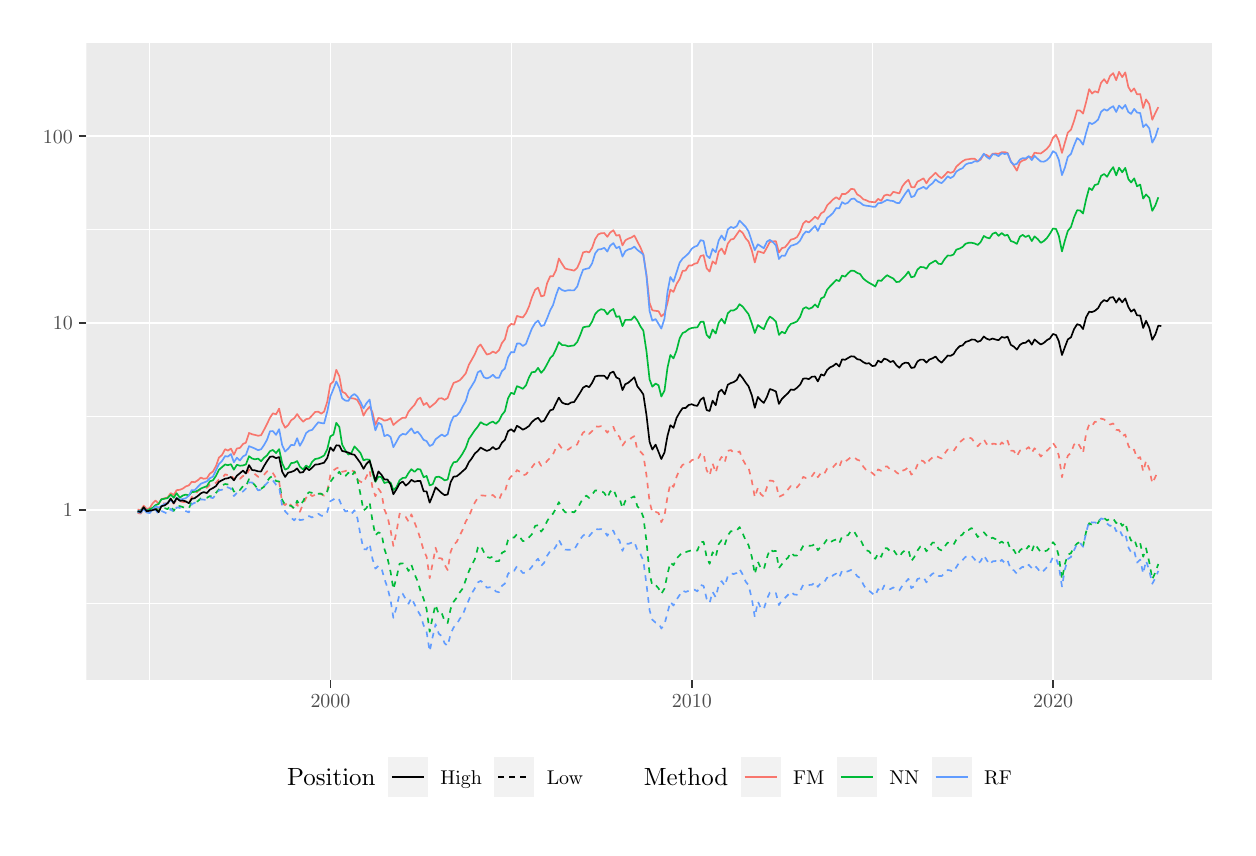
\begin{tikzpicture}[x=1pt,y=1pt]
\definecolor{fillColor}{RGB}{255,255,255}
\path[use as bounding box,fill=fillColor,fill opacity=0.00] (0,0) rectangle (433.62,289.08);
\begin{scope}
\path[clip] (  0.00,  0.00) rectangle (433.62,289.08);
\definecolor{drawColor}{RGB}{255,255,255}
\definecolor{fillColor}{RGB}{255,255,255}

\path[draw=drawColor,line width= 0.6pt,line join=round,line cap=round,fill=fillColor] (  0.00,  0.00) rectangle (433.62,289.08);
\end{scope}
\begin{scope}
\path[clip] ( 21.25, 53.26) rectangle (428.12,283.58);
\definecolor{fillColor}{gray}{0.92}

\path[fill=fillColor] ( 21.25, 53.26) rectangle (428.12,283.58);
\definecolor{drawColor}{RGB}{255,255,255}

\path[draw=drawColor,line width= 0.3pt,line join=round] ( 21.25, 80.97) --
	(428.12, 80.97);

\path[draw=drawColor,line width= 0.3pt,line join=round] ( 21.25,148.54) --
	(428.12,148.54);

\path[draw=drawColor,line width= 0.3pt,line join=round] ( 21.25,216.10) --
	(428.12,216.10);

\path[draw=drawColor,line width= 0.3pt,line join=round] ( 44.12, 53.26) --
	( 44.12,283.58);

\path[draw=drawColor,line width= 0.3pt,line join=round] (174.69, 53.26) --
	(174.69,283.58);

\path[draw=drawColor,line width= 0.3pt,line join=round] (305.25, 53.26) --
	(305.25,283.58);

\path[draw=drawColor,line width= 0.6pt,line join=round] ( 21.25,114.75) --
	(428.12,114.75);

\path[draw=drawColor,line width= 0.6pt,line join=round] ( 21.25,182.32) --
	(428.12,182.32);

\path[draw=drawColor,line width= 0.6pt,line join=round] ( 21.25,249.88) --
	(428.12,249.88);

\path[draw=drawColor,line width= 0.6pt,line join=round] (109.41, 53.26) --
	(109.41,283.58);

\path[draw=drawColor,line width= 0.6pt,line join=round] (239.98, 53.26) --
	(239.98,283.58);

\path[draw=drawColor,line width= 0.6pt,line join=round] (370.52, 53.26) --
	(370.52,283.58);
\definecolor{drawColor}{RGB}{248,118,109}

\path[draw=drawColor,line width= 0.6pt,line join=round] ( 39.74,114.99) --
	( 40.81,114.62) --
	( 41.92,116.34) --
	( 42.99,115.19) --
	( 44.07,115.44) --
	( 45.21,117.27) --
	( 46.21,118.22) --
	( 47.32,117.05) --
	( 48.32,118.69) --
	( 49.50,119.04) --
	( 50.57,119.29) --
	( 51.68,120.89) --
	( 52.79,120.19) --
	( 53.82,121.96) --
	( 54.97,122.09) --
	( 56.04,122.50) --
	( 57.08,123.28) --
	( 58.26,123.71) --
	( 59.29,124.98) --
	( 60.33,124.83) --
	( 61.47,125.52) --
	( 62.58,126.50) --
	( 63.58,126.08) --
	( 64.76,126.26) --
	( 65.84,127.95) --
	( 66.94,128.67) --
	( 68.05,130.65) --
	( 69.09,133.69) --
	( 70.23,134.68) --
	( 71.34,136.75) --
	( 72.34,136.25) --
	( 73.45,136.97) --
	( 74.52,134.76) --
	( 75.59,137.01) --
	( 76.70,137.23) --
	( 77.81,138.64) --
	( 78.85,139.11) --
	( 79.99,142.62) --
	( 81.10,142.16) --
	( 82.10,141.92) --
	( 83.28,141.62) --
	( 84.35,141.82) --
	( 85.35,143.65) --
	( 86.50,145.91) --
	( 87.57,148.16) --
	( 88.60,149.72) --
	( 89.75,149.34) --
	( 90.86,151.43) --
	( 91.96,146.58) --
	( 93.04,144.51) --
	( 94.11,145.45) --
	( 95.22,147.23) --
	( 96.33,147.96) --
	( 97.36,149.46) --
	( 98.36,148.01) --
	( 99.54,146.70) --
	(100.61,147.62) --
	(101.72,147.83) --
	(102.79,148.98) --
	(103.87,150.20) --
	(105.01,150.33) --
	(106.08,149.60) --
	(107.12,150.35) --
	(108.26,153.92) --
	(109.37,160.24) --
	(110.48,161.23) --
	(111.52,165.44) --
	(112.62,163.11) --
	(113.63,157.54) --
	(114.81,156.93) --
	(115.88,155.45) --
	(116.99,155.18) --
	(118.09,155.03) --
	(119.13,154.50) --
	(120.27,152.44) --
	(121.35,148.90) --
	(122.38,150.75) --
	(123.56,152.08) --
	(124.56,150.17) --
	(125.64,145.56) --
	(126.74,148.08) --
	(127.85,147.75) --
	(128.89,147.06) --
	(130.03,147.34) --
	(131.14,147.95) --
	(132.14,145.51) --
	(133.32,146.56) --
	(134.39,147.39) --
	(135.50,148.14) --
	(136.61,148.13) --
	(137.61,150.31) --
	(138.65,151.55) --
	(139.79,152.78) --
	(140.90,154.76) --
	(141.90,155.36) --
	(143.08,152.72) --
	(144.15,153.50) --
	(145.26,151.83) --
	(146.37,152.72) --
	(147.40,153.57) --
	(148.55,155.07) --
	(149.66,155.17) --
	(150.66,154.61) --
	(151.76,155.25) --
	(152.84,158.21) --
	(153.91,160.73) --
	(155.02,161.12) --
	(156.13,161.65) --
	(157.16,162.78) --
	(158.31,164.18) --
	(159.41,167.24) --
	(160.42,169.02) --
	(161.59,171.13) --
	(162.67,173.63) --
	(163.67,174.59) --
	(164.85,172.64) --
	(165.92,170.96) --
	(167.03,171.27) --
	(168.10,172.04) --
	(169.17,171.48) --
	(170.32,172.57) --
	(171.39,175.16) --
	(172.43,176.48) --
	(173.57,180.85) --
	(174.68,182.02) --
	(175.79,181.76) --
	(176.79,184.92) --
	(177.89,184.58) --
	(178.93,184.36) --
	(180.07,185.93) --
	(181.15,188.34) --
	(182.18,191.50) --
	(183.36,194.37) --
	(184.44,195.13) --
	(185.54,192.01) --
	(186.62,192.27) --
	(187.69,196.72) --
	(188.83,199.29) --
	(189.83,199.24) --
	(190.94,201.51) --
	(191.94,205.67) --
	(193.12,203.66) --
	(194.19,202.07) --
	(195.30,201.75) --
	(196.41,201.55) --
	(197.45,201.27) --
	(198.59,202.31) --
	(199.66,204.71) --
	(200.70,207.87) --
	(201.88,208.19) --
	(202.88,207.85) --
	(203.95,209.48) --
	(205.06,212.71) --
	(206.17,214.38) --
	(207.20,214.79) --
	(208.35,214.86) --
	(209.46,213.50) --
	(210.46,215.03) --
	(211.64,215.87) --
	(212.71,213.93) --
	(213.82,214.17) --
	(214.93,210.40) --
	(215.96,212.24) --
	(217.07,212.86) --
	(218.14,213.25) --
	(219.21,213.96) --
	(220.32,211.80) --
	(221.43,209.66) --
	(222.47,207.11) --
	(223.61,199.72) --
	(224.72,189.60) --
	(225.72,186.95) --
	(226.90,186.75) --
	(227.97,186.62) --
	(228.97,184.75) --
	(230.12,185.80) --
	(231.19,189.61) --
	(232.23,194.40) --
	(233.37,193.61) --
	(234.48,196.49) --
	(235.59,198.24) --
	(236.66,201.18) --
	(237.73,201.30) --
	(238.84,203.11) --
	(239.95,203.13) --
	(240.98,203.81) --
	(241.98,204.01) --
	(243.16,206.57) --
	(244.24,206.86) --
	(245.34,202.14) --
	(246.42,200.94) --
	(247.49,204.63) --
	(248.63,203.69) --
	(249.70,208.16) --
	(250.74,209.26) --
	(251.89,207.22) --
	(252.99,211.07) --
	(254.10,212.53) --
	(255.10,212.75) --
	(256.21,214.34) --
	(257.25,215.86) --
	(258.39,214.90) --
	(259.46,212.97) --
	(260.50,211.79) --
	(261.68,208.50) --
	(262.75,204.24) --
	(263.86,208.28) --
	(264.93,207.99) --
	(266.00,207.62) --
	(267.15,209.66) --
	(268.18,211.65) --
	(269.26,211.85) --
	(270.37,211.93) --
	(271.47,207.84) --
	(272.51,209.41) --
	(273.65,209.72) --
	(274.76,211.04) --
	(275.76,212.48) --
	(276.94,212.79) --
	(278.01,213.44) --
	(279.12,215.29) --
	(280.23,218.31) --
	(281.23,219.24) --
	(282.27,218.70) --
	(283.41,219.66) --
	(284.52,220.76) --
	(285.52,219.96) --
	(286.70,222.00) --
	(287.77,222.61) --
	(288.88,224.86) --
	(289.99,225.94) --
	(291.03,227.01) --
	(292.17,227.82) --
	(293.28,227.03) --
	(294.28,229.03) --
	(295.39,228.94) --
	(296.46,229.67) --
	(297.53,230.84) --
	(298.64,230.69) --
	(299.75,228.82) --
	(300.78,228.21) --
	(301.93,227.06) --
	(303.04,226.70) --
	(304.04,226.20) --
	(305.22,226.07) --
	(306.29,226.00) --
	(307.29,227.22) --
	(308.43,226.52) --
	(309.51,228.41) --
	(310.54,228.76) --
	(311.69,228.38) --
	(312.79,229.76) --
	(313.90,229.47) --
	(314.97,229.19) --
	(316.05,231.73) --
	(317.15,233.15) --
	(318.26,234.11) --
	(319.30,231.47) --
	(320.41,231.37) --
	(321.52,233.42) --
	(322.55,233.98) --
	(323.70,234.64) --
	(324.77,232.83) --
	(325.80,234.50) --
	(326.98,235.58) --
	(328.06,236.66) --
	(329.16,235.45) --
	(330.24,234.68) --
	(331.31,235.71) --
	(332.45,236.99) --
	(333.45,236.63) --
	(334.56,237.01) --
	(335.56,238.85) --
	(336.74,239.93) --
	(337.82,240.82) --
	(338.92,241.41) --
	(340.03,241.55) --
	(341.07,241.74) --
	(342.21,241.70) --
	(343.28,240.78) --
	(344.32,241.40) --
	(345.50,243.30) --
	(346.50,243.08) --
	(347.57,242.29) --
	(348.68,243.52) --
	(349.79,243.61) --
	(350.83,243.47) --
	(351.97,244.07) --
	(353.08,244.12) --
	(354.08,243.77) --
	(355.26,240.80) --
	(356.33,239.21) --
	(357.44,237.41) --
	(358.55,240.40) --
	(359.55,241.10) --
	(360.58,241.39) --
	(361.73,242.52) --
	(362.84,242.17) --
	(363.84,243.89) --
	(365.02,243.71) --
	(366.09,243.63) --
	(367.20,244.43) --
	(368.31,245.35) --
	(369.34,246.59) --
	(370.49,249.26) --
	(371.59,250.36) --
	(372.59,248.21) --
	(373.74,243.82) --
	(374.81,247.56) --
	(375.85,251.16) --
	(376.99,252.21) --
	(378.10,255.36) --
	(379.21,259.21) --
	(380.28,259.13) --
	(381.35,258.03) --
	(382.46,262.17) --
	(383.57,266.88) --
	(384.60,265.27) --
	(385.61,266.10) --
	(386.79,265.63) --
	(387.86,269.18) --
	(388.97,270.44) --
	(390.04,268.97) --
	(391.11,271.61) --
	(392.25,272.64) --
	(393.33,270.10) --
	(394.36,273.11) --
	(395.51,271.19) --
	(396.61,272.92) --
	(397.72,267.64) --
	(398.72,265.97) --
	(399.83,267.11) --
	(400.87,265.00) --
	(402.01,265.09) --
	(403.08,260.05) --
	(404.12,263.15) --
	(405.30,261.38) --
	(406.37,255.80) --
	(407.48,258.25) --
	(408.55,260.36);

\path[draw=drawColor,line width= 0.6pt,dash pattern=on 2pt off 2pt ,line join=round] ( 39.74,113.74) --
	( 40.81,113.46) --
	( 41.92,115.11) --
	( 42.99,114.01) --
	( 44.07,114.92) --
	( 45.21,114.74) --
	( 46.21,115.07) --
	( 47.32,115.42) --
	( 48.32,117.13) --
	( 49.50,117.16) --
	( 50.57,117.27) --
	( 51.68,118.16) --
	( 52.79,117.06) --
	( 53.82,118.57) --
	( 54.97,117.96) --
	( 56.04,117.70) --
	( 57.08,117.64) --
	( 58.26,117.21) --
	( 59.29,119.49) --
	( 60.33,119.95) --
	( 61.47,121.64) --
	( 62.58,122.26) --
	( 63.58,122.67) --
	( 64.76,122.83) --
	( 65.84,123.93) --
	( 66.94,123.81) --
	( 68.05,124.65) --
	( 69.09,125.73) --
	( 70.23,126.20) --
	( 71.34,127.68) --
	( 72.34,127.37) --
	( 73.45,127.66) --
	( 74.52,125.86) --
	( 75.59,126.79) --
	( 76.70,126.04) --
	( 77.81,127.12) --
	( 78.85,126.85) --
	( 79.99,129.42) --
	( 81.10,128.56) --
	( 82.10,127.76) --
	( 83.28,126.78) --
	( 84.35,126.84) --
	( 85.35,127.44) --
	( 86.50,128.76) --
	( 87.57,129.02) --
	( 88.60,128.15) --
	( 89.75,126.28) --
	( 90.86,125.19) --
	( 91.96,117.21) --
	( 93.04,116.55) --
	( 94.11,117.80) --
	( 95.22,116.44) --
	( 96.33,114.97) --
	( 97.36,117.16) --
	( 98.36,114.12) --
	( 99.54,117.08) --
	(100.61,119.21) --
	(101.72,120.73) --
	(102.79,119.83) --
	(103.87,120.25) --
	(105.01,121.14) --
	(106.08,120.54) --
	(107.12,119.94) --
	(108.26,121.62) --
	(109.37,127.36) --
	(110.48,129.11) --
	(111.52,129.83) --
	(112.62,130.23) --
	(113.63,128.58) --
	(114.81,128.86) --
	(115.88,129.34) --
	(116.99,129.10) --
	(118.09,128.67) --
	(119.13,125.79) --
	(120.27,125.04) --
	(121.35,124.54) --
	(122.38,126.82) --
	(123.56,129.10) --
	(124.56,123.05) --
	(125.64,119.78) --
	(126.74,122.50) --
	(127.85,120.89) --
	(128.89,115.00) --
	(130.03,112.37) --
	(131.14,107.47) --
	(132.14,101.79) --
	(133.32,107.16) --
	(134.39,113.44) --
	(135.50,112.89) --
	(136.61,112.29) --
	(137.61,110.64) --
	(138.65,113.23) --
	(139.79,110.28) --
	(140.90,107.52) --
	(141.90,104.31) --
	(143.08,100.21) --
	(144.15, 97.91) --
	(145.26, 90.16) --
	(146.37, 95.62) --
	(147.40,101.17) --
	(148.55, 97.43) --
	(149.66, 97.26) --
	(150.66, 95.02) --
	(151.76, 93.09) --
	(152.84, 99.71) --
	(153.91,102.25) --
	(155.02,103.25) --
	(156.13,105.61) --
	(157.16,107.60) --
	(158.31,110.67) --
	(159.41,112.36) --
	(160.42,114.89) --
	(161.59,117.50) --
	(162.67,119.19) --
	(163.67,120.10) --
	(164.85,119.99) --
	(165.92,119.90) --
	(167.03,119.68) --
	(168.10,120.24) --
	(169.17,119.20) --
	(170.32,118.41) --
	(171.39,121.03) --
	(172.43,121.31) --
	(173.57,125.41) --
	(174.68,126.96) --
	(175.79,127.33) --
	(176.79,129.20) --
	(177.89,128.59) --
	(178.93,127.29) --
	(180.07,127.67) --
	(181.15,129.00) --
	(182.18,130.19) --
	(183.36,131.75) --
	(184.44,132.67) --
	(185.54,130.76) --
	(186.62,131.07) --
	(187.69,132.51) --
	(188.83,133.71) --
	(189.83,134.91) --
	(190.94,137.30) --
	(191.94,138.57) --
	(193.12,136.89) --
	(194.19,136.67) --
	(195.30,136.57) --
	(196.41,137.45) --
	(197.45,137.45) --
	(198.59,138.57) --
	(199.66,140.92) --
	(200.70,142.76) --
	(201.88,143.50) --
	(202.88,142.29) --
	(203.95,143.28) --
	(205.06,145.03) --
	(206.17,144.89) --
	(207.20,145.06) --
	(208.35,144.15) --
	(209.46,142.72) --
	(210.46,144.20) --
	(211.64,144.86) --
	(212.71,142.01) --
	(213.82,141.36) --
	(214.93,138.07) --
	(215.96,139.52) --
	(217.07,139.64) --
	(218.14,140.84) --
	(219.21,141.47) --
	(220.32,136.38) --
	(221.43,135.86) --
	(222.47,134.72) --
	(223.61,127.27) --
	(224.72,117.79) --
	(225.72,113.90) --
	(226.90,114.09) --
	(227.97,113.73) --
	(228.97,110.39) --
	(230.12,112.71) --
	(231.19,119.57) --
	(232.23,124.29) --
	(233.37,123.14) --
	(234.48,126.81) --
	(235.59,129.46) --
	(236.66,131.16) --
	(237.73,131.36) --
	(238.84,131.58) --
	(239.95,132.79) --
	(240.98,133.12) --
	(241.98,132.83) --
	(243.16,135.05) --
	(244.24,135.23) --
	(245.34,129.18) --
	(246.42,127.24) --
	(247.49,131.62) --
	(248.63,128.27) --
	(249.70,132.20) --
	(250.74,133.98) --
	(251.89,132.08) --
	(252.99,136.15) --
	(254.10,136.45) --
	(255.10,135.51) --
	(256.21,135.49) --
	(257.25,135.96) --
	(258.39,133.01) --
	(259.46,131.14) --
	(260.50,130.03) --
	(261.68,125.21) --
	(262.75,119.37) --
	(263.86,122.85) --
	(264.93,120.49) --
	(266.00,119.62) --
	(267.15,123.13) --
	(268.18,125.44) --
	(269.26,125.30) --
	(270.37,124.44) --
	(271.47,119.50) --
	(272.51,120.05) --
	(273.65,120.64) --
	(274.76,122.22) --
	(275.76,123.47) --
	(276.94,122.84) --
	(278.01,122.95) --
	(279.12,124.35) --
	(280.23,126.78) --
	(281.23,126.33) --
	(282.27,126.25) --
	(283.41,127.04) --
	(284.52,128.61) --
	(285.52,126.63) --
	(286.70,128.25) --
	(287.77,127.73) --
	(288.88,129.73) --
	(289.99,129.96) --
	(291.03,130.30) --
	(292.17,131.57) --
	(293.28,130.32) --
	(294.28,132.97) --
	(295.39,132.27) --
	(296.46,133.07) --
	(297.53,133.94) --
	(298.64,133.89) --
	(299.75,132.94) --
	(300.78,132.61) --
	(301.93,130.48) --
	(303.04,129.15) --
	(304.04,128.96) --
	(305.22,128.13) --
	(306.29,127.15) --
	(307.29,129.47) --
	(308.43,128.94) --
	(309.51,130.41) --
	(310.54,130.55) --
	(311.69,129.45) --
	(312.79,129.49) --
	(313.90,128.39) --
	(314.97,127.68) --
	(316.05,128.95) --
	(317.15,129.40) --
	(318.26,130.26) --
	(319.30,127.56) --
	(320.41,128.49) --
	(321.52,131.12) --
	(322.55,132.79) --
	(323.70,132.42) --
	(324.77,131.14) --
	(325.80,132.78) --
	(326.98,133.80) --
	(328.06,134.48) --
	(329.16,133.86) --
	(330.24,133.39) --
	(331.31,135.13) --
	(332.45,136.67) --
	(333.45,136.22) --
	(334.56,136.09) --
	(335.56,137.57) --
	(336.74,139.24) --
	(337.82,140.11) --
	(338.92,141.00) --
	(340.03,140.95) --
	(341.07,140.66) --
	(342.21,139.12) --
	(343.28,137.82) --
	(344.32,138.94) --
	(345.50,140.32) --
	(346.50,138.66) --
	(347.57,137.82) --
	(348.68,138.78) --
	(349.79,138.65) --
	(350.83,137.61) --
	(351.97,139.22) --
	(353.08,138.31) --
	(354.08,139.82) --
	(355.26,136.25) --
	(356.33,136.16) --
	(357.44,134.21) --
	(358.55,136.25) --
	(359.55,136.62) --
	(360.58,136.68) --
	(361.73,137.51) --
	(362.84,135.49) --
	(363.84,137.10) --
	(365.02,135.87) --
	(366.09,134.10) --
	(367.20,135.31) --
	(368.31,136.22) --
	(369.34,137.21) --
	(370.49,139.05) --
	(371.59,137.40) --
	(372.59,134.55) --
	(373.74,126.65) --
	(374.81,131.29) --
	(375.85,134.41) --
	(376.99,135.48) --
	(378.10,138.42) --
	(379.21,139.36) --
	(380.28,137.71) --
	(381.35,135.40) --
	(382.46,142.43) --
	(383.57,145.74) --
	(384.60,145.07) --
	(385.61,146.72) --
	(386.79,146.43) --
	(387.86,147.84) --
	(388.97,147.50) --
	(390.04,146.60) --
	(391.11,145.66) --
	(392.25,146.07) --
	(393.33,143.74) --
	(394.36,143.69) --
	(395.51,141.45) --
	(396.61,142.07) --
	(397.72,138.09) --
	(398.72,136.17) --
	(399.83,136.60) --
	(400.87,133.37) --
	(402.01,133.90) --
	(403.08,128.69) --
	(404.12,132.51) --
	(405.30,129.57) --
	(406.37,124.47) --
	(407.48,126.73) --
	(408.55,129.21);
\definecolor{drawColor}{RGB}{0,186,56}

\path[draw=drawColor,line width= 0.6pt,line join=round] ( 39.74,114.45) --
	( 40.81,113.87) --
	( 41.92,115.63) --
	( 42.99,114.22) --
	( 44.07,114.96) --
	( 45.21,115.64) --
	( 46.21,116.55) --
	( 47.32,116.99) --
	( 48.32,118.65) --
	( 49.50,118.87) --
	( 50.57,119.11) --
	( 51.68,120.30) --
	( 52.79,119.21) --
	( 53.82,120.86) --
	( 54.97,119.23) --
	( 56.04,120.02) --
	( 57.08,120.35) --
	( 58.26,120.06) --
	( 59.29,121.29) --
	( 60.33,121.33) --
	( 61.47,121.81) --
	( 62.58,122.55) --
	( 63.58,122.96) --
	( 64.76,123.41) --
	( 65.84,125.18) --
	( 66.94,125.50) --
	( 68.05,127.12) --
	( 69.09,129.30) --
	( 70.23,130.28) --
	( 71.34,131.26) --
	( 72.34,130.97) --
	( 73.45,131.32) --
	( 74.52,129.35) --
	( 75.59,131.13) --
	( 76.70,130.79) --
	( 77.81,130.89) --
	( 78.85,131.24) --
	( 79.99,134.22) --
	( 81.10,133.39) --
	( 82.10,133.11) --
	( 83.28,133.36) --
	( 84.35,132.40) --
	( 85.35,133.61) --
	( 86.50,134.55) --
	( 87.57,136.07) --
	( 88.60,136.48) --
	( 89.75,135.36) --
	( 90.86,136.79) --
	( 91.96,131.71) --
	( 93.04,129.39) --
	( 94.11,129.88) --
	( 95.22,131.74) --
	( 96.33,131.88) --
	( 97.36,132.48) --
	( 98.36,130.46) --
	( 99.54,129.44) --
	(100.61,130.85) --
	(101.72,130.08) --
	(102.79,132.21) --
	(103.87,133.21) --
	(105.01,133.42) --
	(106.08,133.89) --
	(107.12,134.49) --
	(108.26,136.80) --
	(109.37,141.41) --
	(110.48,142.02) --
	(111.52,146.28) --
	(112.62,144.78) --
	(113.63,138.42) --
	(114.81,136.28) --
	(115.88,134.80) --
	(116.99,135.44) --
	(118.09,137.78) --
	(119.13,136.66) --
	(120.27,135.37) --
	(121.35,132.74) --
	(122.38,133.10) --
	(123.56,132.93) --
	(124.56,128.27) --
	(125.64,124.96) --
	(126.74,126.82) --
	(127.85,126.66) --
	(128.89,124.54) --
	(130.03,124.87) --
	(131.14,124.74) --
	(132.14,122.01) --
	(133.32,123.14) --
	(134.39,125.52) --
	(135.50,126.37) --
	(136.61,126.45) --
	(137.61,128.16) --
	(138.65,129.53) --
	(139.79,128.58) --
	(140.90,129.60) --
	(141.90,129.42) --
	(143.08,126.62) --
	(144.15,127.10) --
	(145.26,123.67) --
	(146.37,124.09) --
	(147.40,126.65) --
	(148.55,126.83) --
	(149.66,126.31) --
	(150.66,125.50) --
	(151.76,125.79) --
	(152.84,130.06) --
	(153.91,132.05) --
	(155.02,132.20) --
	(156.13,133.66) --
	(157.16,135.20) --
	(158.31,137.29) --
	(159.41,140.41) --
	(160.42,141.90) --
	(161.59,143.62) --
	(162.67,144.93) --
	(163.67,146.53) --
	(164.85,145.80) --
	(165.92,145.50) --
	(167.03,146.29) --
	(168.10,146.74) --
	(169.17,145.94) --
	(170.32,147.07) --
	(171.39,149.20) --
	(172.43,150.44) --
	(173.57,155.14) --
	(174.68,157.15) --
	(175.79,156.69) --
	(176.79,159.53) --
	(177.89,159.12) --
	(178.93,158.57) --
	(180.07,159.85) --
	(181.15,162.70) --
	(182.18,164.58) --
	(183.36,164.70) --
	(184.44,166.14) --
	(185.54,164.34) --
	(186.62,165.56) --
	(187.69,167.49) --
	(188.83,169.72) --
	(189.83,170.67) --
	(190.94,172.97) --
	(191.94,175.44) --
	(193.12,174.38) --
	(194.19,174.36) --
	(195.30,173.94) --
	(196.41,174.11) --
	(197.45,174.27) --
	(198.59,175.53) --
	(199.66,178.00) --
	(200.70,180.78) --
	(201.88,181.06) --
	(202.88,181.14) --
	(203.95,182.86) --
	(205.06,185.60) --
	(206.17,186.80) --
	(207.20,187.33) --
	(208.35,187.06) --
	(209.46,185.48) --
	(210.46,186.71) --
	(211.64,187.43) --
	(212.71,184.56) --
	(213.82,184.81) --
	(214.93,181.21) --
	(215.96,183.50) --
	(217.07,183.49) --
	(218.14,183.54) --
	(219.21,184.78) --
	(220.32,183.29) --
	(221.43,181.11) --
	(222.47,179.62) --
	(223.61,172.08) --
	(224.72,161.98) --
	(225.72,159.34) --
	(226.90,160.47) --
	(227.97,159.83) --
	(228.97,155.80) --
	(230.12,157.96) --
	(231.19,166.16) --
	(232.23,170.80) --
	(233.37,169.58) --
	(234.48,172.45) --
	(235.59,176.82) --
	(236.66,178.74) --
	(237.73,179.21) --
	(238.84,180.15) --
	(239.95,180.56) --
	(240.98,180.72) --
	(241.98,180.79) --
	(243.16,182.77) --
	(244.24,182.85) --
	(245.34,178.08) --
	(246.42,176.91) --
	(247.49,180.01) --
	(248.63,178.57) --
	(249.70,182.46) --
	(250.74,183.84) --
	(251.89,182.16) --
	(252.99,185.87) --
	(254.10,186.91) --
	(255.10,186.90) --
	(256.21,187.58) --
	(257.25,189.15) --
	(258.39,188.26) --
	(259.46,186.84) --
	(260.50,185.52) --
	(261.68,182.18) --
	(262.75,178.76) --
	(263.86,181.61) --
	(264.93,180.81) --
	(266.00,180.14) --
	(267.15,182.96) --
	(268.18,184.67) --
	(269.26,183.94) --
	(270.37,182.88) --
	(271.47,178.05) --
	(272.51,179.18) --
	(273.65,178.61) --
	(274.76,180.78) --
	(275.76,182.04) --
	(276.94,182.43) --
	(278.01,182.97) --
	(279.12,184.58) --
	(280.23,187.56) --
	(281.23,188.07) --
	(282.27,187.46) --
	(283.41,187.92) --
	(284.52,189.06) --
	(285.52,188.00) --
	(286.70,191.24) --
	(287.77,191.74) --
	(288.88,194.38) --
	(289.99,195.68) --
	(291.03,196.71) --
	(292.17,197.93) --
	(293.28,197.49) --
	(294.28,199.50) --
	(295.39,199.12) --
	(296.46,200.35) --
	(297.53,201.28) --
	(298.64,201.19) --
	(299.75,200.46) --
	(300.78,200.07) --
	(301.93,198.43) --
	(303.04,197.53) --
	(304.04,196.88) --
	(305.22,196.25) --
	(306.29,195.54) --
	(307.29,197.78) --
	(308.43,197.57) --
	(309.51,198.72) --
	(310.54,199.64) --
	(311.69,198.97) --
	(312.79,198.42) --
	(313.90,197.17) --
	(314.97,197.27) --
	(316.05,198.39) --
	(317.15,199.47) --
	(318.26,200.92) --
	(319.30,198.87) --
	(320.41,199.19) --
	(321.52,201.66) --
	(322.55,202.58) --
	(323.70,202.55) --
	(324.77,201.98) --
	(325.80,203.62) --
	(326.98,204.32) --
	(328.06,204.93) --
	(329.16,203.73) --
	(330.24,203.69) --
	(331.31,205.44) --
	(332.45,206.74) --
	(333.45,206.69) --
	(334.56,207.09) --
	(335.56,208.87) --
	(336.74,209.25) --
	(337.82,209.86) --
	(338.92,211.00) --
	(340.03,211.36) --
	(341.07,211.34) --
	(342.21,211.11) --
	(343.28,210.58) --
	(344.32,211.55) --
	(345.50,213.80) --
	(346.50,213.24) --
	(347.57,212.94) --
	(348.68,214.61) --
	(349.79,215.08) --
	(350.83,213.85) --
	(351.97,214.88) --
	(353.08,213.93) --
	(354.08,214.24) --
	(355.26,211.98) --
	(356.33,211.61) --
	(357.44,210.95) --
	(358.55,213.57) --
	(359.55,214.20) --
	(360.58,213.43) --
	(361.73,214.00) --
	(362.84,211.97) --
	(363.84,213.66) --
	(365.02,212.65) --
	(366.09,211.34) --
	(367.20,211.99) --
	(368.31,213.08) --
	(369.34,214.54) --
	(370.49,216.50) --
	(371.59,216.36) --
	(372.59,213.93) --
	(373.74,208.23) --
	(374.81,212.17) --
	(375.85,215.62) --
	(376.99,217.04) --
	(378.10,220.54) --
	(379.21,223.09) --
	(380.28,223.05) --
	(381.35,221.94) --
	(382.46,227.05) --
	(383.57,231.14) --
	(384.60,230.39) --
	(385.61,232.23) --
	(386.79,232.56) --
	(387.86,235.52) --
	(388.97,236.21) --
	(390.04,235.20) --
	(391.11,237.14) --
	(392.25,238.68) --
	(393.33,235.70) --
	(394.36,238.46) --
	(395.51,236.84) --
	(396.61,238.41) --
	(397.72,234.38) --
	(398.72,233.14) --
	(399.83,234.61) --
	(400.87,231.76) --
	(402.01,232.39) --
	(403.08,227.30) --
	(404.12,228.81) --
	(405.30,227.59) --
	(406.37,222.90) --
	(407.48,224.87) --
	(408.55,227.78);

\path[draw=drawColor,line width= 0.6pt,dash pattern=on 2pt off 2pt ,line join=round] ( 39.74,113.88) --
	( 40.81,114.65) --
	( 41.92,115.76) --
	( 42.99,114.63) --
	( 44.07,115.09) --
	( 45.21,115.22) --
	( 46.21,115.51) --
	( 47.32,114.40) --
	( 48.32,115.53) --
	( 49.50,115.46) --
	( 50.57,115.11) --
	( 51.68,116.43) --
	( 52.79,114.45) --
	( 53.82,116.25) --
	( 54.97,116.20) --
	( 56.04,115.83) --
	( 57.08,115.53) --
	( 58.26,115.46) --
	( 59.29,117.60) --
	( 60.33,117.56) --
	( 61.47,117.97) --
	( 62.58,118.98) --
	( 63.58,119.09) --
	( 64.76,119.20) --
	( 65.84,119.82) --
	( 66.94,119.73) --
	( 68.05,120.98) --
	( 69.09,122.21) --
	( 70.23,123.64) --
	( 71.34,124.18) --
	( 72.34,124.03) --
	( 73.45,123.83) --
	( 74.52,121.43) --
	( 75.59,122.43) --
	( 76.70,122.01) --
	( 77.81,123.40) --
	( 78.85,123.27) --
	( 79.99,125.95) --
	( 81.10,124.88) --
	( 82.10,123.76) --
	( 83.28,122.26) --
	( 84.35,122.49) --
	( 85.35,123.15) --
	( 86.50,125.15) --
	( 87.57,126.55) --
	( 88.60,127.03) --
	( 89.75,125.25) --
	( 90.86,125.11) --
	( 91.96,118.44) --
	( 93.04,116.68) --
	( 94.11,116.49) --
	( 95.22,116.27) --
	( 96.33,115.41) --
	( 97.36,118.15) --
	( 98.36,116.55) --
	( 99.54,117.94) --
	(100.61,120.29) --
	(101.72,121.23) --
	(102.79,120.98) --
	(103.87,120.62) --
	(105.01,120.64) --
	(106.08,120.66) --
	(107.12,120.06) --
	(108.26,121.54) --
	(109.37,124.94) --
	(110.48,126.46) --
	(111.52,127.38) --
	(112.62,128.60) --
	(113.63,126.86) --
	(114.81,127.06) --
	(115.88,128.25) --
	(116.99,126.95) --
	(118.09,128.66) --
	(119.13,125.89) --
	(120.27,120.42) --
	(121.35,114.58) --
	(122.38,115.45) --
	(123.56,117.55) --
	(124.56,111.10) --
	(125.64,105.60) --
	(126.74,106.69) --
	(127.85,106.32) --
	(128.89,100.79) --
	(130.03, 97.33) --
	(131.14, 92.43) --
	(132.14, 86.16) --
	(133.32, 90.53) --
	(134.39, 95.41) --
	(135.50, 95.52) --
	(136.61, 94.75) --
	(137.61, 92.73) --
	(138.65, 95.05) --
	(139.79, 91.63) --
	(140.90, 89.06) --
	(141.90, 85.67) --
	(143.08, 82.67) --
	(144.15, 78.93) --
	(145.26, 70.80) --
	(146.37, 76.38) --
	(147.40, 80.57) --
	(148.55, 77.07) --
	(149.66, 77.42) --
	(150.66, 74.70) --
	(151.76, 73.95) --
	(152.84, 79.08) --
	(153.91, 81.62) --
	(155.02, 83.09) --
	(156.13, 85.00) --
	(157.16, 86.40) --
	(158.31, 89.54) --
	(159.41, 92.59) --
	(160.42, 94.82) --
	(161.59, 97.02) --
	(162.67,101.16) --
	(163.67,102.00) --
	(164.85, 99.55) --
	(165.92, 97.84) --
	(167.03, 97.47) --
	(168.10, 97.98) --
	(169.17, 96.28) --
	(170.32, 96.34) --
	(171.39, 99.35) --
	(172.43, 99.84) --
	(173.57,103.94) --
	(174.68,104.88) --
	(175.79,104.84) --
	(176.79,106.07) --
	(177.89,104.96) --
	(178.93,103.52) --
	(180.07,103.81) --
	(181.15,104.90) --
	(182.18,106.01) --
	(183.36,109.04) --
	(184.44,109.29) --
	(185.54,106.98) --
	(186.62,108.35) --
	(187.69,110.75) --
	(188.83,112.58) --
	(189.83,113.48) --
	(190.94,115.42) --
	(191.94,117.65) --
	(193.12,115.28) --
	(194.19,114.05) --
	(195.30,113.59) --
	(196.41,114.18) --
	(197.45,113.94) --
	(198.59,115.19) --
	(199.66,117.21) --
	(200.70,119.06) --
	(201.88,119.98) --
	(202.88,119.14) --
	(203.95,120.31) --
	(205.06,121.87) --
	(206.17,121.80) --
	(207.20,121.74) --
	(208.35,120.94) --
	(209.46,119.15) --
	(210.46,121.40) --
	(211.64,122.30) --
	(212.71,119.68) --
	(213.82,119.17) --
	(214.93,115.45) --
	(215.96,118.08) --
	(217.07,118.42) --
	(218.14,119.22) --
	(219.21,119.73) --
	(220.32,116.10) --
	(221.43,114.92) --
	(222.47,112.22) --
	(223.61,103.46) --
	(224.72, 91.67) --
	(225.72, 87.55) --
	(226.90, 87.70) --
	(227.97, 86.46) --
	(228.97, 84.49) --
	(230.12, 86.41) --
	(231.19, 91.66) --
	(232.23, 95.80) --
	(233.37, 94.85) --
	(234.48, 97.26) --
	(235.59, 98.40) --
	(236.66, 99.71) --
	(237.73, 99.57) --
	(238.84, 99.92) --
	(239.95,100.25) --
	(240.98,100.31) --
	(241.98,100.10) --
	(243.16,103.18) --
	(244.24,103.30) --
	(245.34, 97.79) --
	(246.42, 95.34) --
	(247.49, 99.53) --
	(248.63, 97.80) --
	(249.70,102.49) --
	(250.74,103.85) --
	(251.89,102.21) --
	(252.99,105.61) --
	(254.10,107.15) --
	(255.10,106.93) --
	(256.21,107.38) --
	(257.25,108.62) --
	(258.39,106.30) --
	(259.46,103.76) --
	(260.50,102.06) --
	(261.68, 97.82) --
	(262.75, 91.63) --
	(263.86, 96.10) --
	(264.93, 93.74) --
	(266.00, 93.32) --
	(267.15, 97.62) --
	(268.18,100.59) --
	(269.26, 99.87) --
	(270.37,100.03) --
	(271.47, 93.83) --
	(272.51, 95.17) --
	(273.65, 96.65) --
	(274.76, 97.57) --
	(275.76, 99.46) --
	(276.94, 98.32) --
	(278.01, 98.37) --
	(279.12, 99.82) --
	(280.23,101.82) --
	(281.23,102.02) --
	(282.27,101.88) --
	(283.41,101.91) --
	(284.52,102.48) --
	(285.52,100.25) --
	(286.70,101.69) --
	(287.77,102.60) --
	(288.88,104.22) --
	(289.99,103.12) --
	(291.03,103.73) --
	(292.17,104.14) --
	(293.28,102.81) --
	(294.28,105.17) --
	(295.39,105.51) --
	(296.46,105.67) --
	(297.53,107.36) --
	(298.64,106.98) --
	(299.75,105.16) --
	(300.78,104.34) --
	(301.93,101.99) --
	(303.04,100.26) --
	(304.04, 99.86) --
	(305.22, 98.30) --
	(306.29, 97.12) --
	(307.29, 99.16) --
	(308.43, 97.87) --
	(309.51,100.95) --
	(310.54,100.99) --
	(311.69, 99.82) --
	(312.79,100.42) --
	(313.90, 98.82) --
	(314.97, 97.86) --
	(316.05, 99.46) --
	(317.15,100.25) --
	(318.26,100.36) --
	(319.30, 96.32) --
	(320.41, 97.85) --
	(321.52,100.13) --
	(322.55,101.58) --
	(323.70,101.88) --
	(324.77, 99.85) --
	(325.80,101.40) --
	(326.98,103.03) --
	(328.06,102.93) --
	(329.16,100.74) --
	(330.24,100.18) --
	(331.31,101.54) --
	(332.45,103.05) --
	(333.45,102.41) --
	(334.56,102.25) --
	(335.56,104.07) --
	(336.74,105.27) --
	(337.82,105.93) --
	(338.92,107.76) --
	(340.03,107.57) --
	(341.07,108.30) --
	(342.21,106.98) --
	(343.28,105.03) --
	(344.32,105.77) --
	(345.50,106.76) --
	(346.50,105.59) --
	(347.57,104.34) --
	(348.68,104.78) --
	(349.79,104.24) --
	(350.83,102.66) --
	(351.97,103.37) --
	(353.08,102.52) --
	(354.08,103.45) --
	(355.26,100.18) --
	(356.33,100.37) --
	(357.44, 98.32) --
	(358.55,100.20) --
	(359.55,101.00) --
	(360.58,100.26) --
	(361.73,101.84) --
	(362.84, 99.78) --
	(363.84,102.58) --
	(365.02,101.00) --
	(366.09, 99.53) --
	(367.20, 99.78) --
	(368.31,100.16) --
	(369.34,101.16) --
	(370.49,103.17) --
	(371.59,101.77) --
	(372.59, 98.12) --
	(373.74, 89.78) --
	(374.81, 95.30) --
	(375.85, 98.63) --
	(376.99, 99.19) --
	(378.10,101.48) --
	(379.21,102.68) --
	(380.28,103.26) --
	(381.35,101.69) --
	(382.46,106.88) --
	(383.57,110.04) --
	(384.60,109.42) --
	(385.61,109.92) --
	(386.79,110.10) --
	(387.86,112.12) --
	(388.97,111.87) --
	(390.04,111.02) --
	(391.11,111.65) --
	(392.25,111.67) --
	(393.33,110.05) --
	(394.36,110.98) --
	(395.51,109.06) --
	(396.61,110.19) --
	(397.72,106.25) --
	(398.72,103.70) --
	(399.83,104.37) --
	(400.87,101.32) --
	(402.01,102.79) --
	(403.08, 97.92) --
	(404.12,100.96) --
	(405.30, 95.87) --
	(406.37, 89.78) --
	(407.48, 92.22) --
	(408.55, 95.27);
\definecolor{drawColor}{RGB}{97,156,255}

\path[draw=drawColor,line width= 0.6pt,line join=round] ( 39.74,114.16) --
	( 40.81,113.77) --
	( 41.92,115.15) --
	( 42.99,113.90) --
	( 44.07,113.66) --
	( 45.21,114.98) --
	( 46.21,116.11) --
	( 47.32,115.61) --
	( 48.32,116.26) --
	( 49.50,116.97) --
	( 50.57,117.31) --
	( 51.68,118.45) --
	( 52.79,117.29) --
	( 53.82,119.10) --
	( 54.97,118.55) --
	( 56.04,118.76) --
	( 57.08,119.03) --
	( 58.26,119.97) --
	( 59.29,121.99) --
	( 60.33,121.92) --
	( 61.47,123.16) --
	( 62.58,124.29) --
	( 63.58,124.68) --
	( 64.76,125.16) --
	( 65.84,126.28) --
	( 66.94,126.81) --
	( 68.05,129.13) --
	( 69.09,131.36) --
	( 70.23,132.51) --
	( 71.34,134.28) --
	( 72.34,134.07) --
	( 73.45,135.01) --
	( 74.52,132.04) --
	( 75.59,133.69) --
	( 76.70,132.68) --
	( 77.81,134.16) --
	( 78.85,134.69) --
	( 79.99,137.84) --
	( 81.10,137.42) --
	( 82.10,137.00) --
	( 83.28,136.40) --
	( 84.35,136.74) --
	( 85.35,138.16) --
	( 86.50,140.21) --
	( 87.57,143.25) --
	( 88.60,143.31) --
	( 89.75,141.95) --
	( 90.86,144.01) --
	( 91.96,138.22) --
	( 93.04,135.91) --
	( 94.11,136.92) --
	( 95.22,138.32) --
	( 96.33,138.19) --
	( 97.36,140.74) --
	( 98.36,137.99) --
	( 99.54,140.05) --
	(100.61,142.58) --
	(101.72,143.45) --
	(102.79,143.73) --
	(103.87,145.11) --
	(105.01,146.49) --
	(106.08,146.21) --
	(107.12,146.06) --
	(108.26,150.43) --
	(109.37,155.82) --
	(110.48,158.49) --
	(111.52,161.23) --
	(112.62,158.84) --
	(113.63,155.17) --
	(114.81,154.31) --
	(115.88,154.21) --
	(116.99,155.97) --
	(118.09,156.71) --
	(119.13,155.76) --
	(120.27,153.80) --
	(121.35,151.51) --
	(122.38,153.31) --
	(123.56,154.70) --
	(124.56,148.59) --
	(125.64,143.57) --
	(126.74,146.29) --
	(127.85,145.67) --
	(128.89,141.46) --
	(130.03,141.98) --
	(131.14,141.18) --
	(132.14,137.49) --
	(133.32,139.56) --
	(134.39,141.50) --
	(135.50,142.29) --
	(136.61,142.05) --
	(137.61,143.15) --
	(138.65,144.30) --
	(139.79,142.46) --
	(140.90,143.11) --
	(141.90,141.93) --
	(143.08,140.13) --
	(144.15,139.69) --
	(145.26,137.90) --
	(146.37,138.47) --
	(147.40,140.35) --
	(148.55,141.23) --
	(149.66,142.08) --
	(150.66,141.38) --
	(151.76,142.16) --
	(152.84,146.27) --
	(153.91,148.58) --
	(155.02,148.85) --
	(156.13,150.15) --
	(157.16,152.20) --
	(158.31,154.17) --
	(159.41,157.94) --
	(160.42,159.54) --
	(161.59,161.51) --
	(162.67,164.55) --
	(163.67,165.14) --
	(164.85,162.78) --
	(165.92,162.33) --
	(167.03,162.77) --
	(168.10,163.67) --
	(169.17,162.56) --
	(170.32,162.57) --
	(171.39,164.99) --
	(172.43,165.89) --
	(173.57,169.93) --
	(174.68,171.86) --
	(175.79,171.73) --
	(176.79,174.93) --
	(177.89,174.96) --
	(178.93,174.04) --
	(180.07,174.84) --
	(181.15,177.70) --
	(182.18,180.32) --
	(183.36,182.33) --
	(184.44,183.24) --
	(185.54,181.25) --
	(186.62,181.60) --
	(187.69,184.04) --
	(188.83,186.98) --
	(189.83,188.82) --
	(190.94,192.47) --
	(191.94,195.17) --
	(193.12,194.25) --
	(194.19,193.93) --
	(195.30,194.21) --
	(196.41,194.16) --
	(197.45,194.16) --
	(198.59,195.55) --
	(199.66,198.89) --
	(200.70,201.62) --
	(201.88,201.96) --
	(202.88,202.16) --
	(203.95,203.89) --
	(205.06,207.50) --
	(206.17,208.94) --
	(207.20,209.03) --
	(208.35,209.52) --
	(209.46,208.19) --
	(210.46,210.30) --
	(211.64,211.22) --
	(212.71,209.39) --
	(213.82,209.97) --
	(214.93,206.35) --
	(215.96,208.32) --
	(217.07,208.97) --
	(218.14,209.22) --
	(219.21,209.97) --
	(220.32,208.76) --
	(221.43,207.95) --
	(222.47,207.06) --
	(223.61,199.24) --
	(224.72,186.72) --
	(225.72,183.19) --
	(226.90,183.79) --
	(227.97,182.03) --
	(228.97,180.33) --
	(230.12,183.97) --
	(231.19,193.51) --
	(232.23,198.98) --
	(233.37,197.27) --
	(234.48,200.69) --
	(235.59,204.16) --
	(236.66,205.63) --
	(237.73,206.51) --
	(238.84,207.55) --
	(239.95,209.21) --
	(240.98,209.91) --
	(241.98,210.30) --
	(243.16,212.29) --
	(244.24,212.02) --
	(245.34,206.78) --
	(246.42,205.79) --
	(247.49,209.10) --
	(248.63,207.93) --
	(249.70,212.20) --
	(250.74,213.98) --
	(251.89,212.22) --
	(252.99,216.18) --
	(254.10,217.07) --
	(255.10,216.68) --
	(256.21,217.35) --
	(257.25,219.35) --
	(258.39,218.20) --
	(259.46,217.09) --
	(260.50,215.45) --
	(261.68,211.81) --
	(262.75,208.69) --
	(263.86,210.80) --
	(264.93,210.08) --
	(266.00,209.37) --
	(267.15,211.78) --
	(268.18,212.38) --
	(269.26,211.64) --
	(270.37,210.41) --
	(271.47,205.49) --
	(272.51,206.73) --
	(273.65,206.63) --
	(274.76,208.94) --
	(275.76,210.25) --
	(276.94,210.62) --
	(278.01,211.04) --
	(279.12,212.15) --
	(280.23,214.27) --
	(281.23,215.44) --
	(282.27,215.10) --
	(283.41,216.32) --
	(284.52,217.45) --
	(285.52,215.63) --
	(286.70,218.15) --
	(287.77,218.10) --
	(288.88,220.34) --
	(289.99,221.15) --
	(291.03,222.15) --
	(292.17,223.90) --
	(293.28,223.78) --
	(294.28,226.04) --
	(295.39,225.37) --
	(296.46,225.89) --
	(297.53,227.13) --
	(298.64,227.35) --
	(299.75,226.30) --
	(300.78,225.90) --
	(301.93,224.99) --
	(303.04,224.72) --
	(304.04,224.63) --
	(305.22,224.40) --
	(306.29,224.33) --
	(307.29,225.64) --
	(308.43,225.73) --
	(309.51,226.29) --
	(310.54,226.86) --
	(311.69,226.56) --
	(312.79,226.43) --
	(313.90,225.77) --
	(314.97,225.67) --
	(316.05,227.44) --
	(317.15,229.16) --
	(318.26,230.59) --
	(319.30,227.83) --
	(320.41,228.29) --
	(321.52,230.51) --
	(322.55,230.98) --
	(323.70,231.55) --
	(324.77,230.75) --
	(325.80,231.98) --
	(326.98,232.86) --
	(328.06,234.25) --
	(329.16,233.35) --
	(330.24,232.91) --
	(331.31,233.99) --
	(332.45,235.37) --
	(333.45,234.73) --
	(334.56,235.38) --
	(335.56,237.07) --
	(336.74,237.84) --
	(337.82,238.31) --
	(338.92,239.63) --
	(340.03,240.11) --
	(341.07,240.20) --
	(342.21,240.79) --
	(343.28,240.70) --
	(344.32,241.77) --
	(345.50,243.53) --
	(346.50,242.42) --
	(347.57,241.68) --
	(348.68,243.35) --
	(349.79,243.21) --
	(350.83,242.63) --
	(351.97,243.74) --
	(353.08,243.40) --
	(354.08,243.70) --
	(355.26,240.66) --
	(356.33,239.54) --
	(357.44,239.88) --
	(358.55,241.41) --
	(359.55,241.95) --
	(360.58,241.82) --
	(361.73,242.66) --
	(362.84,241.21) --
	(363.84,242.75) --
	(365.02,241.62) --
	(366.09,240.71) --
	(367.20,240.65) --
	(368.31,241.22) --
	(369.34,242.28) --
	(370.49,244.45) --
	(371.59,243.73) --
	(372.59,241.37) --
	(373.74,235.81) --
	(374.81,238.57) --
	(375.85,242.38) --
	(376.99,243.46) --
	(378.10,246.54) --
	(379.21,249.18) --
	(380.28,248.40) --
	(381.35,246.79) --
	(382.46,251.05) --
	(383.57,254.79) --
	(384.60,254.26) --
	(385.61,254.81) --
	(386.79,255.86) --
	(387.86,258.64) --
	(388.97,259.61) --
	(390.04,259.08) --
	(391.11,260.02) --
	(392.25,260.70) --
	(393.33,258.61) --
	(394.36,260.92) --
	(395.51,259.78) --
	(396.61,261.16) --
	(397.72,258.60) --
	(398.72,257.92) --
	(399.83,259.74) --
	(400.87,258.41) --
	(402.01,258.23) --
	(403.08,253.15) --
	(404.12,254.18) --
	(405.30,252.67) --
	(406.37,247.54) --
	(407.48,249.58) --
	(408.55,252.91);

\path[draw=drawColor,line width= 0.6pt,dash pattern=on 2pt off 2pt ,line join=round] ( 39.74,114.34) --
	( 40.81,114.35) --
	( 41.92,116.06) --
	( 42.99,114.32) --
	( 44.07,114.83) --
	( 45.21,114.89) --
	( 46.21,114.91) --
	( 47.32,113.28) --
	( 48.32,114.45) --
	( 49.50,113.94) --
	( 50.57,113.34) --
	( 51.68,115.23) --
	( 52.79,113.92) --
	( 53.82,115.75) --
	( 54.97,115.59) --
	( 56.04,114.87) --
	( 57.08,114.41) --
	( 58.26,113.95) --
	( 59.29,116.86) --
	( 60.33,117.40) --
	( 61.47,117.63) --
	( 62.58,118.61) --
	( 63.58,118.54) --
	( 64.76,118.38) --
	( 65.84,119.34) --
	( 66.94,119.10) --
	( 68.05,120.37) --
	( 69.09,121.90) --
	( 70.23,122.09) --
	( 71.34,123.24) --
	( 72.34,122.95) --
	( 73.45,122.51) --
	( 74.52,119.82) --
	( 75.59,120.97) --
	( 76.70,121.01) --
	( 77.81,121.50) --
	( 78.85,122.52) --
	( 79.99,124.79) --
	( 81.10,124.73) --
	( 82.10,123.50) --
	( 83.28,121.88) --
	( 84.35,122.18) --
	( 85.35,123.30) --
	( 86.50,124.46) --
	( 87.57,125.64) --
	( 88.60,125.49) --
	( 89.75,123.93) --
	( 90.86,123.17) --
	( 91.96,116.18) --
	( 93.04,114.32) --
	( 94.11,113.19) --
	( 95.22,111.98) --
	( 96.33,111.04) --
	( 97.36,112.47) --
	( 98.36,111.12) --
	( 99.54,111.31) --
	(100.61,112.37) --
	(101.72,112.57) --
	(102.79,112.08) --
	(103.87,112.68) --
	(105.01,113.45) --
	(106.08,112.73) --
	(107.12,112.72) --
	(108.26,114.13) --
	(109.37,117.98) --
	(110.48,118.57) --
	(111.52,119.37) --
	(112.62,118.42) --
	(113.63,115.90) --
	(114.81,114.27) --
	(115.88,114.49) --
	(116.99,113.34) --
	(118.09,114.68) --
	(119.13,111.92) --
	(120.27,105.68) --
	(121.35,100.65) --
	(122.38,100.54) --
	(123.56,102.57) --
	(124.56, 97.27) --
	(125.64, 93.59) --
	(126.74, 94.62) --
	(127.85, 93.80) --
	(128.89, 89.97) --
	(130.03, 86.71) --
	(131.14, 82.18) --
	(132.14, 75.81) --
	(133.32, 79.79) --
	(134.39, 84.60) --
	(135.50, 84.53) --
	(136.61, 82.59) --
	(137.61, 80.91) --
	(138.65, 82.98) --
	(139.79, 80.67) --
	(140.90, 78.45) --
	(141.90, 76.71) --
	(143.08, 73.11) --
	(144.15, 70.74) --
	(145.26, 63.73) --
	(146.37, 69.08) --
	(147.40, 73.53) --
	(148.55, 70.10) --
	(149.66, 69.18) --
	(150.66, 66.62) --
	(151.76, 65.71) --
	(152.84, 70.00) --
	(153.91, 72.38) --
	(155.02, 73.48) --
	(156.13, 75.46) --
	(157.16, 76.78) --
	(158.31, 79.73) --
	(159.41, 82.28) --
	(160.42, 84.61) --
	(161.59, 86.47) --
	(162.67, 88.62) --
	(163.67, 89.18) --
	(164.85, 88.32) --
	(165.92, 86.71) --
	(167.03, 86.87) --
	(168.10, 86.75) --
	(169.17, 85.36) --
	(170.32, 85.07) --
	(171.39, 87.40) --
	(172.43, 88.18) --
	(173.57, 91.65) --
	(174.68, 92.95) --
	(175.79, 92.81) --
	(176.79, 94.45) --
	(177.89, 93.28) --
	(178.93, 92.02) --
	(180.07, 92.23) --
	(181.15, 93.06) --
	(182.18, 94.26) --
	(183.36, 96.11) --
	(184.44, 97.18) --
	(185.54, 94.60) --
	(186.62, 95.74) --
	(187.69, 98.24) --
	(188.83, 99.98) --
	(189.83, 99.97) --
	(190.94,101.76) --
	(191.94,103.98) --
	(193.12,101.76) --
	(194.19,100.47) --
	(195.30,100.44) --
	(196.41,100.42) --
	(197.45,100.44) --
	(198.59,102.35) --
	(199.66,104.25) --
	(200.70,105.53) --
	(201.88,106.35) --
	(202.88,105.34) --
	(203.95,106.59) --
	(205.06,107.96) --
	(206.17,107.78) --
	(207.20,107.90) --
	(208.35,107.24) --
	(209.46,105.47) --
	(210.46,107.37) --
	(211.64,107.32) --
	(212.71,104.64) --
	(213.82,103.86) --
	(214.93,100.01) --
	(215.96,102.61) --
	(217.07,102.56) --
	(218.14,102.93) --
	(219.21,103.40) --
	(220.32,100.19) --
	(221.43, 98.88) --
	(222.47, 96.53) --
	(223.61, 87.85) --
	(224.72, 78.63) --
	(225.72, 75.14) --
	(226.90, 74.10) --
	(227.97, 73.96) --
	(228.97, 71.95) --
	(230.12, 73.57) --
	(231.19, 77.62) --
	(232.23, 81.61) --
	(233.37, 80.26) --
	(234.48, 82.40) --
	(235.59, 84.09) --
	(236.66, 85.70) --
	(237.73, 85.17) --
	(238.84, 85.57) --
	(239.95, 85.93) --
	(240.98, 85.99) --
	(241.98, 85.40) --
	(243.16, 87.69) --
	(244.24, 87.37) --
	(245.34, 82.72) --
	(246.42, 81.20) --
	(247.49, 85.22) --
	(248.63, 83.25) --
	(249.70, 87.65) --
	(250.74, 89.10) --
	(251.89, 87.42) --
	(252.99, 90.89) --
	(254.10, 91.95) --
	(255.10, 91.64) --
	(256.21, 92.06) --
	(257.25, 93.46) --
	(258.39, 91.44) --
	(259.46, 88.89) --
	(260.50, 87.61) --
	(261.68, 82.65) --
	(262.75, 76.12) --
	(263.86, 81.73) --
	(264.93, 79.26) --
	(266.00, 78.98) --
	(267.15, 82.71) --
	(268.18, 84.97) --
	(269.26, 84.86) --
	(270.37, 84.76) --
	(271.47, 80.44) --
	(272.51, 82.25) --
	(273.65, 83.02) --
	(274.76, 84.13) --
	(275.76, 85.25) --
	(276.94, 84.26) --
	(278.01, 84.15) --
	(279.12, 85.53) --
	(280.23, 87.72) --
	(281.23, 87.79) --
	(282.27, 87.69) --
	(283.41, 87.78) --
	(284.52, 88.65) --
	(285.52, 87.02) --
	(286.70, 88.57) --
	(287.77, 88.61) --
	(288.88, 90.39) --
	(289.99, 89.94) --
	(291.03, 91.23) --
	(292.17, 91.82) --
	(293.28, 90.44) --
	(294.28, 92.86) --
	(295.39, 92.30) --
	(296.46, 92.66) --
	(297.53, 93.12) --
	(298.64, 92.40) --
	(299.75, 90.87) --
	(300.78, 90.23) --
	(301.93, 87.95) --
	(303.04, 86.06) --
	(304.04, 85.64) --
	(305.22, 84.63) --
	(306.29, 83.82) --
	(307.29, 86.22) --
	(308.43, 85.10) --
	(309.51, 87.50) --
	(310.54, 87.24) --
	(311.69, 86.18) --
	(312.79, 86.80) --
	(313.90, 86.12) --
	(314.97, 85.69) --
	(316.05, 87.46) --
	(317.15, 88.63) --
	(318.26, 89.92) --
	(319.30, 86.57) --
	(320.41, 87.35) --
	(321.52, 89.85) --
	(322.55, 90.16) --
	(323.70, 90.52) --
	(324.77, 88.64) --
	(325.80, 90.68) --
	(326.98, 91.80) --
	(328.06, 92.15) --
	(329.16, 90.97) --
	(330.24, 90.89) --
	(331.31, 91.89) --
	(332.45, 93.13) --
	(333.45, 92.92) --
	(334.56, 92.45) --
	(335.56, 94.17) --
	(336.74, 95.98) --
	(337.82, 96.70) --
	(338.92, 97.89) --
	(340.03, 97.99) --
	(341.07, 98.21) --
	(342.21, 96.95) --
	(343.28, 95.40) --
	(344.32, 96.26) --
	(345.50, 98.40) --
	(346.50, 96.80) --
	(347.57, 95.13) --
	(348.68, 96.23) --
	(349.79, 96.36) --
	(350.83, 95.55) --
	(351.97, 96.80) --
	(353.08, 95.66) --
	(354.08, 96.62) --
	(355.26, 93.25) --
	(356.33, 93.02) --
	(357.44, 91.75) --
	(358.55, 93.57) --
	(359.55, 94.30) --
	(360.58, 93.68) --
	(361.73, 94.98) --
	(362.84, 93.77) --
	(363.84, 94.78) --
	(365.02, 93.53) --
	(366.09, 92.09) --
	(367.20, 92.91) --
	(368.31, 94.13) --
	(369.34, 95.27) --
	(370.49, 97.82) --
	(371.59, 97.29) --
	(372.59, 94.66) --
	(373.74, 87.15) --
	(374.81, 93.36) --
	(375.85, 97.06) --
	(376.99, 97.82) --
	(378.10,100.29) --
	(379.21,102.57) --
	(380.28,102.95) --
	(381.35,101.51) --
	(382.46,106.58) --
	(383.57,110.79) --
	(384.60,110.27) --
	(385.61,110.33) --
	(386.79,109.74) --
	(387.86,111.78) --
	(388.97,111.40) --
	(390.04,109.87) --
	(391.11,108.99) --
	(392.25,109.68) --
	(393.33,107.12) --
	(394.36,108.02) --
	(395.51,105.54) --
	(396.61,106.39) --
	(397.72,101.35) --
	(398.72, 99.45) --
	(399.83,100.07) --
	(400.87, 95.79) --
	(402.01, 96.85) --
	(403.08, 91.82) --
	(404.12, 96.49) --
	(405.30, 92.84) --
	(406.37, 88.14) --
	(407.48, 90.19) --
	(408.55, 92.73);
\definecolor{drawColor}{RGB}{0,0,0}

\path[draw=drawColor,line width= 0.6pt,line join=round] ( 39.74,114.35) --
	( 40.81,114.05) --
	( 41.92,115.79) --
	( 42.99,114.36) --
	( 44.07,114.51) --
	( 45.21,114.76) --
	( 46.21,115.11) --
	( 47.32,114.00) --
	( 48.32,116.16) --
	( 49.50,116.46) --
	( 50.57,117.22) --
	( 51.68,118.93) --
	( 52.79,117.25) --
	( 53.82,119.08) --
	( 54.97,118.13) --
	( 56.04,118.20) --
	( 57.08,117.93) --
	( 58.26,117.24) --
	( 59.29,118.84) --
	( 60.33,119.06) --
	( 61.47,119.86) --
	( 62.58,120.81) --
	( 63.58,121.27) --
	( 64.76,120.91) --
	( 65.84,122.15) --
	( 66.94,122.71) --
	( 68.05,123.46) --
	( 69.09,124.92) --
	( 70.23,125.56) --
	( 71.34,126.12) --
	( 72.34,126.25) --
	( 73.45,126.73) --
	( 74.52,125.50) --
	( 75.59,127.18) --
	( 76.70,128.08) --
	( 77.81,129.03) --
	( 78.85,127.98) --
	( 79.99,131.01) --
	( 81.10,129.22) --
	( 82.10,129.12) --
	( 83.28,128.75) --
	( 84.35,128.71) --
	( 85.35,130.58) --
	( 86.50,132.46) --
	( 87.57,134.00) --
	( 88.60,134.15) --
	( 89.75,133.52) --
	( 90.86,133.93) --
	( 91.96,128.65) --
	( 93.04,126.73) --
	( 94.11,128.29) --
	( 95.22,128.54) --
	( 96.33,128.97) --
	( 97.36,129.82) --
	( 98.36,128.27) --
	( 99.54,128.48) --
	(100.61,130.04) --
	(101.72,129.17) --
	(102.79,130.08) --
	(103.87,131.19) --
	(105.01,131.29) --
	(106.08,131.58) --
	(107.12,131.89) --
	(108.26,133.60) --
	(109.37,137.39) --
	(110.48,136.14) --
	(111.52,138.17) --
	(112.62,138.09) --
	(113.63,136.13) --
	(114.81,135.84) --
	(115.88,135.55) --
	(116.99,134.98) --
	(118.09,134.74) --
	(119.13,133.31) --
	(120.27,131.75) --
	(121.35,129.67) --
	(122.38,131.40) --
	(123.56,132.56) --
	(124.56,129.31) --
	(125.64,125.28) --
	(126.74,128.71) --
	(127.85,127.50) --
	(128.89,125.85) --
	(130.03,125.78) --
	(131.14,123.99) --
	(132.14,120.48) --
	(133.32,122.36) --
	(134.39,124.34) --
	(135.50,125.09) --
	(136.61,123.62) --
	(137.61,124.41) --
	(138.65,125.68) --
	(139.79,125.01) --
	(140.90,125.27) --
	(141.90,125.29) --
	(143.08,121.55) --
	(144.15,121.50) --
	(145.26,117.44) --
	(146.37,120.14) --
	(147.40,122.99) --
	(148.55,121.90) --
	(149.66,120.86) --
	(150.66,120.17) --
	(151.76,120.40) --
	(152.84,124.87) --
	(153.91,126.84) --
	(155.02,126.96) --
	(156.13,127.85) --
	(157.16,128.80) --
	(158.31,129.79) --
	(159.41,132.07) --
	(160.42,133.36) --
	(161.59,135.22) --
	(162.67,136.14) --
	(163.67,137.35) --
	(164.85,136.66) --
	(165.92,136.15) --
	(167.03,136.57) --
	(168.10,137.53) --
	(169.17,136.67) --
	(170.32,137.19) --
	(171.39,139.15) --
	(172.43,140.09) --
	(173.57,143.24) --
	(174.68,143.98) --
	(175.79,143.06) --
	(176.79,145.21) --
	(177.89,144.59) --
	(178.93,143.81) --
	(180.07,144.39) --
	(181.15,145.12) --
	(182.18,146.56) --
	(183.36,147.56) --
	(184.44,148.11) --
	(185.54,146.64) --
	(186.62,147.04) --
	(187.69,148.93) --
	(188.83,150.82) --
	(189.83,151.11) --
	(190.94,153.44) --
	(191.94,155.39) --
	(193.12,153.60) --
	(194.19,153.12) --
	(195.30,152.99) --
	(196.41,153.66) --
	(197.45,153.79) --
	(198.59,155.54) --
	(199.66,157.24) --
	(200.70,159.00) --
	(201.88,159.69) --
	(202.88,159.18) --
	(203.95,160.71) --
	(205.06,163.04) --
	(206.17,163.31) --
	(207.20,163.28) --
	(208.35,163.27) --
	(209.46,162.15) --
	(210.46,164.25) --
	(211.64,164.82) --
	(212.71,162.71) --
	(213.82,162.15) --
	(214.93,158.13) --
	(215.96,160.26) --
	(217.07,160.80) --
	(218.14,161.75) --
	(219.21,162.75) --
	(220.32,159.46) --
	(221.43,158.08) --
	(222.47,156.54) --
	(223.61,149.01) --
	(224.72,139.40) --
	(225.72,136.63) --
	(226.90,138.41) --
	(227.97,135.73) --
	(228.97,133.22) --
	(230.12,135.57) --
	(231.19,141.58) --
	(232.23,145.41) --
	(233.37,144.49) --
	(234.48,148.09) --
	(235.59,150.03) --
	(236.66,151.61) --
	(237.73,151.63) --
	(238.84,152.72) --
	(239.95,153.01) --
	(240.98,152.58) --
	(241.98,152.43) --
	(243.16,154.65) --
	(244.24,155.45) --
	(245.34,150.89) --
	(246.42,150.57) --
	(247.49,154.29) --
	(248.63,152.65) --
	(249.70,157.37) --
	(250.74,158.28) --
	(251.89,156.58) --
	(252.99,160.06) --
	(254.10,160.67) --
	(255.10,161.00) --
	(256.21,161.76) --
	(257.25,163.84) --
	(258.39,162.44) --
	(259.46,160.81) --
	(260.50,159.46) --
	(261.68,156.20) --
	(262.75,151.73) --
	(263.86,155.64) --
	(264.93,154.39) --
	(266.00,153.48) --
	(267.15,155.71) --
	(268.18,158.51) --
	(269.26,158.13) --
	(270.37,157.62) --
	(271.47,153.11) --
	(272.51,154.89) --
	(273.65,156.01) --
	(274.76,157.03) --
	(275.76,158.33) --
	(276.94,158.17) --
	(278.01,158.98) --
	(279.12,160.07) --
	(280.23,162.25) --
	(281.23,162.36) --
	(282.27,162.08) --
	(283.41,162.96) --
	(284.52,163.02) --
	(285.52,161.25) --
	(286.70,163.80) --
	(287.77,163.34) --
	(288.88,165.39) --
	(289.99,166.37) --
	(291.03,166.81) --
	(292.17,167.75) --
	(293.28,166.65) --
	(294.28,169.22) --
	(295.39,169.08) --
	(296.46,169.73) --
	(297.53,170.33) --
	(298.64,170.24) --
	(299.75,169.28) --
	(300.78,169.10) --
	(301.93,168.21) --
	(303.04,167.69) --
	(304.04,167.84) --
	(305.22,166.79) --
	(306.29,166.96) --
	(307.29,168.77) --
	(308.43,168.10) --
	(309.51,169.49) --
	(310.54,169.14) --
	(311.69,168.26) --
	(312.79,168.66) --
	(313.90,167.12) --
	(314.97,166.19) --
	(316.05,167.54) --
	(317.15,168.06) --
	(318.26,167.88) --
	(319.30,166.11) --
	(320.41,166.32) --
	(321.52,168.45) --
	(322.55,169.12) --
	(323.70,169.12) --
	(324.77,168.06) --
	(325.80,169.15) --
	(326.98,169.60) --
	(328.06,170.25) --
	(329.16,168.85) --
	(330.24,168.03) --
	(331.31,169.27) --
	(332.45,170.60) --
	(333.45,170.48) --
	(334.56,171.10) --
	(335.56,172.71) --
	(336.74,173.97) --
	(337.82,174.27) --
	(338.92,175.51) --
	(340.03,175.86) --
	(341.07,176.38) --
	(342.21,176.34) --
	(343.28,175.56) --
	(344.32,175.92) --
	(345.50,177.48) --
	(346.50,176.69) --
	(347.57,176.31) --
	(348.68,176.75) --
	(349.79,176.38) --
	(350.83,176.17) --
	(351.97,177.30) --
	(353.08,177.04) --
	(354.08,177.44) --
	(355.26,174.47) --
	(356.33,173.85) --
	(357.44,172.75) --
	(358.55,174.43) --
	(359.55,175.10) --
	(360.58,175.21) --
	(361.73,176.19) --
	(362.84,174.53) --
	(363.84,176.41) --
	(365.02,175.39) --
	(366.09,174.59) --
	(367.20,175.18) --
	(368.31,176.18) --
	(369.34,176.74) --
	(370.49,178.39) --
	(371.59,178.00) --
	(372.59,175.83) --
	(373.74,170.79) --
	(374.81,173.68) --
	(375.85,176.42) --
	(376.99,177.19) --
	(378.10,180.13) --
	(379.21,181.93) --
	(380.28,181.59) --
	(381.35,180.17) --
	(382.46,184.46) --
	(383.57,186.42) --
	(384.60,186.32) --
	(385.61,186.75) --
	(386.79,187.72) --
	(387.86,189.66) --
	(388.97,190.65) --
	(390.04,190.16) --
	(391.11,191.52) --
	(392.25,191.72) --
	(393.33,189.73) --
	(394.36,191.35) --
	(395.51,189.84) --
	(396.61,191.24) --
	(397.72,188.15) --
	(398.72,186.49) --
	(399.83,187.30) --
	(400.87,185.11) --
	(402.01,185.09) --
	(403.08,180.56) --
	(404.12,183.16) --
	(405.30,180.62) --
	(406.37,176.29) --
	(407.48,178.26) --
	(408.55,181.40) --
	(409.63,181.26);
\end{scope}
\begin{scope}
\path[clip] (  0.00,  0.00) rectangle (433.62,289.08);
\definecolor{drawColor}{gray}{0.30}

\node[text=drawColor,anchor=base east,inner sep=0pt, outer sep=0pt, scale=  0.72] at ( 16.30,112.28) {1};

\node[text=drawColor,anchor=base east,inner sep=0pt, outer sep=0pt, scale=  0.72] at ( 16.30,179.84) {10};

\node[text=drawColor,anchor=base east,inner sep=0pt, outer sep=0pt, scale=  0.72] at ( 16.30,247.40) {100};
\end{scope}
\begin{scope}
\path[clip] (  0.00,  0.00) rectangle (433.62,289.08);
\definecolor{drawColor}{gray}{0.20}

\path[draw=drawColor,line width= 0.6pt,line join=round] ( 18.50,114.75) --
	( 21.25,114.75);

\path[draw=drawColor,line width= 0.6pt,line join=round] ( 18.50,182.32) --
	( 21.25,182.32);

\path[draw=drawColor,line width= 0.6pt,line join=round] ( 18.50,249.88) --
	( 21.25,249.88);
\end{scope}
\begin{scope}
\path[clip] (  0.00,  0.00) rectangle (433.62,289.08);
\definecolor{drawColor}{gray}{0.20}

\path[draw=drawColor,line width= 0.6pt,line join=round] (109.41, 50.51) --
	(109.41, 53.26);

\path[draw=drawColor,line width= 0.6pt,line join=round] (239.98, 50.51) --
	(239.98, 53.26);

\path[draw=drawColor,line width= 0.6pt,line join=round] (370.52, 50.51) --
	(370.52, 53.26);
\end{scope}
\begin{scope}
\path[clip] (  0.00,  0.00) rectangle (433.62,289.08);
\definecolor{drawColor}{gray}{0.30}

\node[text=drawColor,anchor=base,inner sep=0pt, outer sep=0pt, scale=  0.72] at (109.41, 43.35) {2000};

\node[text=drawColor,anchor=base,inner sep=0pt, outer sep=0pt, scale=  0.72] at (239.98, 43.35) {2010};

\node[text=drawColor,anchor=base,inner sep=0pt, outer sep=0pt, scale=  0.72] at (370.52, 43.35) {2020};
\end{scope}
\begin{scope}
\path[clip] (  0.00,  0.00) rectangle (433.62,289.08);
\definecolor{fillColor}{RGB}{255,255,255}

\path[fill=fillColor] ( 88.25,  5.50) rectangle (206.17, 30.95);
\end{scope}
\begin{scope}
\path[clip] (  0.00,  0.00) rectangle (433.62,289.08);
\definecolor{drawColor}{RGB}{0,0,0}

\node[text=drawColor,anchor=base west,inner sep=0pt, outer sep=0pt, scale=  0.90] at ( 93.75, 15.13) {Position};
\end{scope}
\begin{scope}
\path[clip] (  0.00,  0.00) rectangle (433.62,289.08);
\definecolor{fillColor}{gray}{0.95}

\path[fill=fillColor] (130.17, 11.00) rectangle (144.62, 25.45);
\end{scope}
\begin{scope}
\path[clip] (  0.00,  0.00) rectangle (433.62,289.08);
\definecolor{drawColor}{RGB}{0,0,0}

\path[draw=drawColor,line width= 0.6pt,line join=round] (131.61, 18.23) -- (143.18, 18.23);
\end{scope}
\begin{scope}
\path[clip] (  0.00,  0.00) rectangle (433.62,289.08);
\definecolor{fillColor}{gray}{0.95}

\path[fill=fillColor] (168.62, 11.00) rectangle (183.07, 25.45);
\end{scope}
\begin{scope}
\path[clip] (  0.00,  0.00) rectangle (433.62,289.08);
\definecolor{drawColor}{RGB}{0,0,0}

\path[draw=drawColor,line width= 0.6pt,dash pattern=on 2pt off 2pt ,line join=round] (170.06, 18.23) -- (181.63, 18.23);
\end{scope}
\begin{scope}
\path[clip] (  0.00,  0.00) rectangle (433.62,289.08);
\definecolor{drawColor}{RGB}{0,0,0}

\node[text=drawColor,anchor=base west,inner sep=0pt, outer sep=0pt, scale=  0.72] at (149.12, 15.75) {High};
\end{scope}
\begin{scope}
\path[clip] (  0.00,  0.00) rectangle (433.62,289.08);
\definecolor{drawColor}{RGB}{0,0,0}

\node[text=drawColor,anchor=base west,inner sep=0pt, outer sep=0pt, scale=  0.72] at (187.57, 15.75) {Low};
\end{scope}
\begin{scope}
\path[clip] (  0.00,  0.00) rectangle (433.62,289.08);
\definecolor{fillColor}{RGB}{255,255,255}

\path[fill=fillColor] (217.17,  5.50) rectangle (361.12, 30.95);
\end{scope}
\begin{scope}
\path[clip] (  0.00,  0.00) rectangle (433.62,289.08);
\definecolor{drawColor}{RGB}{0,0,0}

\node[text=drawColor,anchor=base west,inner sep=0pt, outer sep=0pt, scale=  0.90] at (222.67, 15.13) {Method};
\end{scope}
\begin{scope}
\path[clip] (  0.00,  0.00) rectangle (433.62,289.08);
\definecolor{fillColor}{gray}{0.95}

\path[fill=fillColor] (257.66, 11.00) rectangle (272.12, 25.45);
\end{scope}
\begin{scope}
\path[clip] (  0.00,  0.00) rectangle (433.62,289.08);
\definecolor{drawColor}{RGB}{248,118,109}

\path[draw=drawColor,line width= 0.6pt,line join=round] (259.11, 18.23) -- (270.67, 18.23);
\end{scope}
\begin{scope}
\path[clip] (  0.00,  0.00) rectangle (433.62,289.08);
\definecolor{fillColor}{gray}{0.95}

\path[fill=fillColor] (292.41, 11.00) rectangle (306.87, 25.45);
\end{scope}
\begin{scope}
\path[clip] (  0.00,  0.00) rectangle (433.62,289.08);
\definecolor{drawColor}{RGB}{0,186,56}

\path[draw=drawColor,line width= 0.6pt,line join=round] (293.86, 18.23) -- (305.42, 18.23);
\end{scope}
\begin{scope}
\path[clip] (  0.00,  0.00) rectangle (433.62,289.08);
\definecolor{fillColor}{gray}{0.95}

\path[fill=fillColor] (326.66, 11.00) rectangle (341.12, 25.45);
\end{scope}
\begin{scope}
\path[clip] (  0.00,  0.00) rectangle (433.62,289.08);
\definecolor{drawColor}{RGB}{97,156,255}

\path[draw=drawColor,line width= 0.6pt,line join=round] (328.11, 18.23) -- (339.67, 18.23);
\end{scope}
\begin{scope}
\path[clip] (  0.00,  0.00) rectangle (433.62,289.08);
\definecolor{drawColor}{RGB}{0,0,0}

\node[text=drawColor,anchor=base west,inner sep=0pt, outer sep=0pt, scale=  0.72] at (276.62, 15.75) {FM};
\end{scope}
\begin{scope}
\path[clip] (  0.00,  0.00) rectangle (433.62,289.08);
\definecolor{drawColor}{RGB}{0,0,0}

\node[text=drawColor,anchor=base west,inner sep=0pt, outer sep=0pt, scale=  0.72] at (311.37, 15.75) {NN};
\end{scope}
\begin{scope}
\path[clip] (  0.00,  0.00) rectangle (433.62,289.08);
\definecolor{drawColor}{RGB}{0,0,0}

\node[text=drawColor,anchor=base west,inner sep=0pt, outer sep=0pt, scale=  0.72] at (345.62, 15.75) {RF};
\end{scope}
\end{tikzpicture}

\label{plot:cumul_ew_portf_return}
\end{figure}

It is quite expected that the predictability of the value-weighted portfolios is lower than the equal-weighted portfolios. One reason for this is that the stocks are divided into ten expected return portfolios. From Table \ref{table:CountrySummary} it can be seen that on an average month dataset contains approximately 340 stocks. This would mean that even if stocks were allocated to portfolios evenly, each portfolio would on average contain 34 stocks. This can be considered sufficient diversification for an equal-weighted portfolio. Nevertheless, typical to stock markets also Nordic stock markets have few extremely large market capitalization companies. The performance of these companies can even after winsorizing the market value drive the performance of the whole portfolio if the number of stocks inside the portfolio is limited. \par

Additionally, it is not guaranteed that each expected return portfolio would consist of the same amount of stocks. This is because breakpoint expected returns for the portfolio allocation are calculated from the expected returns of large market capitalization stocks. The distribution of the expected returns of the small market value companies does not necessarily follow the expected return distribution of the large market value companies, which could lead to unbalanced portfolios. This can further lower the diversification of the portfolios. One alternative to ensure diversification of the machine learning portfolios would be to allocate stocks to only five expected return portfolios instead of ten. \par

\begin{figure}[ht]
\centering
\caption[Cumulative return of value weighted machine learning portfolios]{\textbf{Cumulative return of value weighted machine learning portfolios \textnormal{- Own source}}\\ Figure plots the realized historical cumulative excess return of the out-of-sample predictions. The figure shows the performance of portfolios that are formed allocating all except micro-cap stocks to ten portfolios based on their expected returns. Re-allocation is done monthly. Section \ref{Methodology} describes how expected returns are derived for different models. FM stands for linear regression model, RF stands for random forest model and NN stands for neural network model. The solid line plots the cumulative performance of the highest expected return portfolio whereas the dashed line plots the cumulative excess return for the lowest expected return portfolio. All portfolios are value-weighted. The solid black line shows the value-weighted market return. All returns are converted to US dollars. The prediction period spans from July 1994 to November 2022.}
% Created by tikzDevice version 0.12.6 on 2024-03-11 19:47:34
% !TEX encoding = UTF-8 Unicode
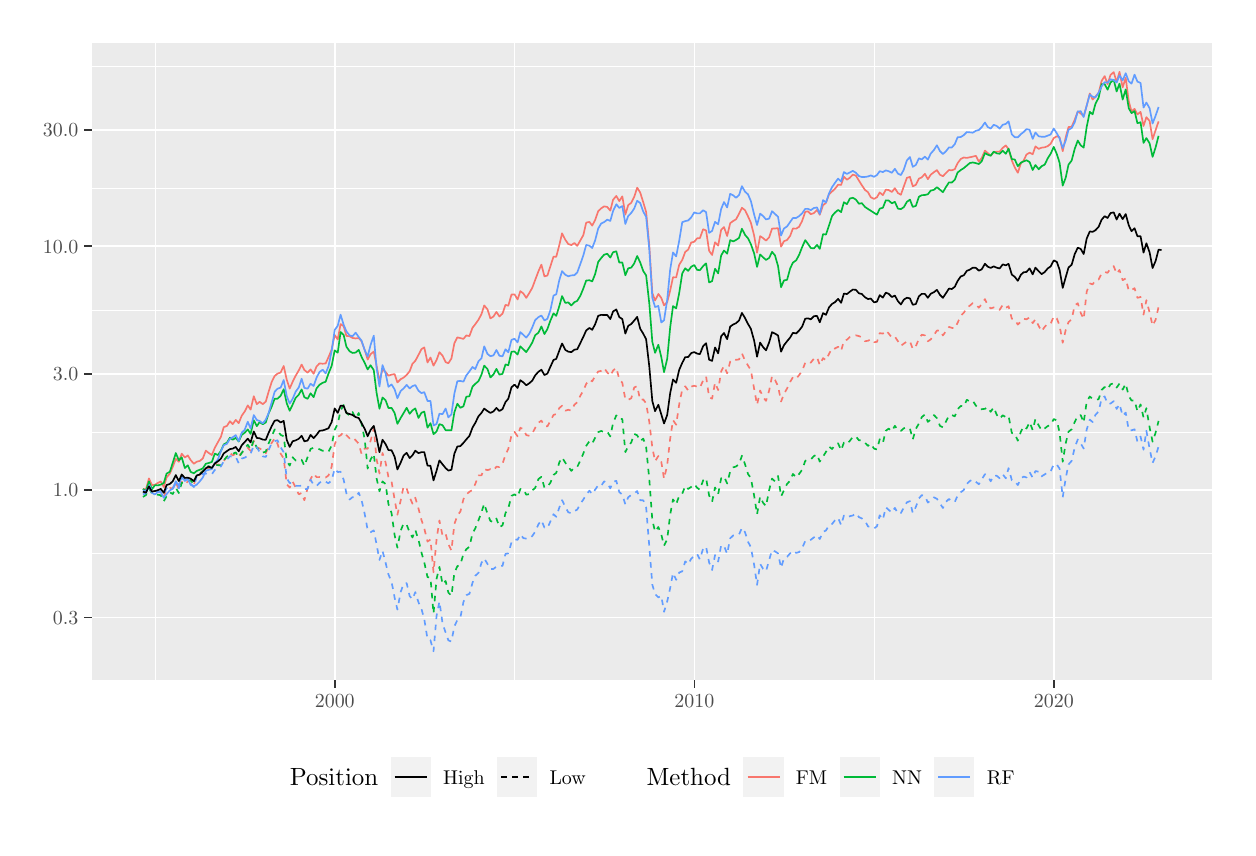
\begin{tikzpicture}[x=1pt,y=1pt]
\definecolor{fillColor}{RGB}{255,255,255}
\path[use as bounding box,fill=fillColor,fill opacity=0.00] (0,0) rectangle (433.62,289.08);
\begin{scope}
\path[clip] (  0.00,  0.00) rectangle (433.62,289.08);
\definecolor{drawColor}{RGB}{255,255,255}
\definecolor{fillColor}{RGB}{255,255,255}

\path[draw=drawColor,line width= 0.6pt,line join=round,line cap=round,fill=fillColor] (  0.00,  0.00) rectangle (433.62,289.08);
\end{scope}
\begin{scope}
\path[clip] ( 23.25, 53.26) rectangle (428.12,283.58);
\definecolor{fillColor}{gray}{0.92}

\path[fill=fillColor] ( 23.25, 53.26) rectangle (428.12,283.58);
\definecolor{drawColor}{RGB}{255,255,255}

\path[draw=drawColor,line width= 0.3pt,line join=round] ( 23.25, 98.94) --
	(428.12, 98.94);

\path[draw=drawColor,line width= 0.3pt,line join=round] ( 23.25,142.99) --
	(428.12,142.99);

\path[draw=drawColor,line width= 0.3pt,line join=round] ( 23.25,187.05) --
	(428.12,187.05);

\path[draw=drawColor,line width= 0.3pt,line join=round] ( 23.25,231.10) --
	(428.12,231.10);

\path[draw=drawColor,line width= 0.3pt,line join=round] ( 23.25,275.16) --
	(428.12,275.16);

\path[draw=drawColor,line width= 0.3pt,line join=round] ( 46.01, 53.26) --
	( 46.01,283.58);

\path[draw=drawColor,line width= 0.3pt,line join=round] (175.94, 53.26) --
	(175.94,283.58);

\path[draw=drawColor,line width= 0.3pt,line join=round] (305.86, 53.26) --
	(305.86,283.58);

\path[draw=drawColor,line width= 0.6pt,line join=round] ( 23.25, 75.90) --
	(428.12, 75.90);

\path[draw=drawColor,line width= 0.6pt,line join=round] ( 23.25,121.97) --
	(428.12,121.97);

\path[draw=drawColor,line width= 0.6pt,line join=round] ( 23.25,164.01) --
	(428.12,164.01);

\path[draw=drawColor,line width= 0.6pt,line join=round] ( 23.25,210.08) --
	(428.12,210.08);

\path[draw=drawColor,line width= 0.6pt,line join=round] ( 23.25,252.12) --
	(428.12,252.12);

\path[draw=drawColor,line width= 0.6pt,line join=round] (110.97, 53.26) --
	(110.97,283.58);

\path[draw=drawColor,line width= 0.6pt,line join=round] (240.91, 53.26) --
	(240.91,283.58);

\path[draw=drawColor,line width= 0.6pt,line join=round] (370.80, 53.26) --
	(370.80,283.58);
\definecolor{drawColor}{RGB}{248,118,109}

\path[draw=drawColor,line width= 0.6pt,line join=round] ( 41.65,122.42) --
	( 42.72,122.18) --
	( 43.82,126.20) --
	( 44.89,123.83) --
	( 45.95,123.88) --
	( 47.09,124.60) --
	( 48.09,125.11) --
	( 49.19,123.09) --
	( 50.19,126.54) --
	( 51.36,127.93) --
	( 52.43,130.39) --
	( 53.53,133.30) --
	( 54.63,132.20) --
	( 55.66,135.15) --
	( 56.80,133.77) --
	( 57.87,134.50) --
	( 58.90,132.81) --
	( 60.07,131.50) --
	( 61.11,132.26) --
	( 62.14,132.48) --
	( 63.28,133.40) --
	( 64.38,136.24) --
	( 65.37,135.43) --
	( 66.55,134.64) --
	( 67.62,137.26) --
	( 68.72,139.26) --
	( 69.82,141.21) --
	( 70.85,144.73) --
	( 71.99,145.17) --
	( 73.09,146.86) --
	( 74.09,145.81) --
	( 75.19,147.34) --
	( 76.26,146.17) --
	( 77.33,148.82) --
	( 78.43,150.39) --
	( 79.53,152.61) --
	( 80.56,151.05) --
	( 81.70,155.90) --
	( 82.80,153.02) --
	( 83.80,153.87) --
	( 84.97,153.05) --
	( 86.04,153.95) --
	( 87.04,157.44) --
	( 88.17,161.04) --
	( 89.24,163.20) --
	( 90.27,164.06) --
	( 91.41,164.49) --
	( 92.51,166.83) --
	( 93.62,161.81) --
	( 94.68,158.66) --
	( 95.75,161.12) --
	( 96.85,163.33) --
	( 97.96,165.24) --
	( 98.99,167.33) --
	( 99.98,165.38) --
	(101.16,164.42) --
	(102.22,165.60) --
	(103.33,164.03) --
	(104.39,166.68) --
	(105.46,167.77) --
	(106.60,167.65) --
	(107.67,167.75) --
	(108.70,170.00) --
	(109.84,172.77) --
	(110.94,178.03) --
	(112.04,176.41) --
	(113.07,181.99) --
	(114.18,181.22) --
	(115.17,177.69) --
	(116.34,177.58) --
	(117.41,176.96) --
	(118.51,176.78) --
	(119.62,176.94) --
	(120.65,175.74) --
	(121.79,172.61) --
	(122.85,169.14) --
	(123.89,171.07) --
	(125.06,172.05) --
	(126.06,167.04) --
	(127.12,161.38) --
	(128.22,165.61) --
	(129.33,164.66) --
	(130.36,163.32) --
	(131.50,163.72) --
	(132.60,163.89) --
	(133.60,160.89) --
	(134.77,162.05) --
	(135.84,162.63) --
	(136.94,163.59) --
	(138.04,164.97) --
	(139.04,167.62) --
	(140.07,168.69) --
	(141.21,170.82) --
	(142.31,172.93) --
	(143.31,173.54) --
	(144.48,168.08) --
	(145.55,169.88) --
	(146.65,166.96) --
	(147.75,168.98) --
	(148.78,171.82) --
	(149.92,170.54) --
	(151.02,168.24) --
	(152.02,167.81) --
	(153.12,169.53) --
	(154.19,175.06) --
	(155.26,177.16) --
	(156.36,176.91) --
	(157.46,176.61) --
	(158.49,177.86) --
	(159.63,177.64) --
	(160.73,180.63) --
	(161.73,181.91) --
	(162.90,183.54) --
	(163.97,185.54) --
	(164.97,188.71) --
	(166.14,187.31) --
	(167.21,184.01) --
	(168.31,184.70) --
	(169.38,186.37) --
	(170.45,184.73) --
	(171.58,185.74) --
	(172.65,188.92) --
	(173.68,188.61) --
	(174.82,192.64) --
	(175.92,192.72) --
	(177.03,190.87) --
	(178.02,193.87) --
	(179.12,193.02) --
	(180.16,191.43) --
	(181.29,193.25) --
	(182.36,195.13) --
	(183.39,197.93) --
	(184.57,201.05) --
	(185.63,203.46) --
	(186.74,199.19) --
	(187.80,199.52) --
	(188.87,202.83) --
	(190.01,206.35) --
	(191.00,206.31) --
	(192.11,210.53) --
	(193.10,214.77) --
	(194.28,212.43) --
	(195.34,210.90) --
	(196.45,210.52) --
	(197.55,211.26) --
	(198.58,210.23) --
	(199.72,212.23) --
	(200.79,214.13) --
	(201.82,218.63) --
	(202.99,218.89) --
	(203.99,217.56) --
	(205.05,219.58) --
	(206.16,222.78) --
	(207.26,223.80) --
	(208.29,224.51) --
	(209.43,224.29) --
	(210.53,222.95) --
	(211.53,226.90) --
	(212.70,228.27) --
	(213.77,226.41) --
	(214.87,228.13) --
	(215.97,221.54) --
	(217.00,224.95) --
	(218.11,225.81) --
	(219.17,227.92) --
	(220.24,231.26) --
	(221.34,229.49) --
	(222.45,225.94) --
	(223.48,222.45) --
	(224.62,210.36) --
	(225.72,193.17) --
	(226.71,190.50) --
	(227.89,192.85) --
	(228.96,191.41) --
	(229.95,188.73) --
	(231.09,189.89) --
	(232.16,194.09) --
	(233.19,198.88) --
	(234.33,198.83) --
	(235.43,203.41) --
	(236.53,205.16) --
	(237.60,208.04) --
	(238.67,208.88) --
	(239.77,211.44) --
	(240.87,211.71) --
	(241.90,212.97) --
	(242.90,213.02) --
	(244.07,216.23) --
	(245.14,215.82) --
	(246.24,208.44) --
	(247.31,206.95) --
	(248.38,211.55) --
	(249.51,210.31) --
	(250.58,216.05) --
	(251.61,217.03) --
	(252.75,213.80) --
	(253.85,218.43) --
	(254.96,219.25) --
	(255.95,219.81) --
	(257.06,221.85) --
	(258.09,223.99) --
	(259.22,223.12) --
	(260.29,220.89) --
	(261.32,218.63) --
	(262.50,213.98) --
	(263.56,207.76) --
	(264.67,213.74) --
	(265.73,213.04) --
	(266.80,212.13) --
	(267.94,213.34) --
	(268.97,216.47) --
	(270.04,216.52) --
	(271.14,216.62) --
	(272.24,209.94) --
	(273.27,211.91) --
	(274.41,212.36) --
	(275.52,213.84) --
	(276.51,216.50) --
	(277.69,216.45) --
	(278.75,217.13) --
	(279.85,219.25) --
	(280.96,222.54) --
	(281.95,222.72) --
	(282.98,221.69) --
	(284.12,222.07) --
	(285.23,223.23) --
	(286.22,221.48) --
	(287.40,224.91) --
	(288.46,225.78) --
	(289.57,228.87) --
	(290.67,229.89) --
	(291.70,230.83) --
	(292.84,232.33) --
	(293.94,232.25) --
	(294.94,235.24) --
	(296.04,234.13) --
	(297.11,234.87) --
	(298.17,236.00) --
	(299.28,235.60) --
	(300.38,233.80) --
	(301.41,232.16) --
	(302.55,230.46) --
	(303.65,229.62) --
	(304.65,227.78) --
	(305.82,227.20) --
	(306.89,227.81) --
	(307.88,229.52) --
	(309.02,228.57) --
	(310.09,230.53) --
	(311.12,230.40) --
	(312.26,229.70) --
	(313.36,231.06) --
	(314.46,229.32) --
	(315.53,228.70) --
	(316.60,231.74) --
	(317.70,234.81) --
	(318.80,235.17) --
	(319.83,231.76) --
	(320.94,232.27) --
	(322.04,234.51) --
	(323.07,234.99) --
	(324.21,236.28) --
	(325.28,234.33) --
	(326.31,235.95) --
	(327.48,236.86) --
	(328.55,237.61) --
	(329.65,235.91) --
	(330.72,235.41) --
	(331.79,236.51) --
	(332.92,237.65) --
	(333.92,237.51) --
	(335.02,237.97) --
	(336.02,240.11) --
	(337.19,241.65) --
	(338.26,242.16) --
	(339.36,242.01) --
	(340.46,242.26) --
	(341.50,242.47) --
	(342.63,242.77) --
	(343.70,240.70) --
	(344.73,241.95) --
	(345.91,244.65) --
	(346.90,243.79) --
	(347.97,242.84) --
	(349.07,244.02) --
	(350.17,244.29) --
	(351.21,244.27) --
	(352.34,245.66) --
	(353.45,246.51) --
	(354.44,245.17) --
	(355.62,241.09) --
	(356.68,238.58) --
	(357.79,236.65) --
	(358.89,240.07) --
	(359.88,241.02) --
	(360.92,243.24) --
	(362.05,243.91) --
	(363.16,243.34) --
	(364.15,246.18) --
	(365.33,245.29) --
	(366.39,245.72) --
	(367.50,245.85) --
	(368.60,246.28) --
	(369.63,247.11) --
	(370.77,249.18) --
	(371.87,249.84) --
	(372.87,249.47) --
	(374.01,244.46) --
	(375.07,249.38) --
	(376.10,253.16) --
	(377.24,253.28) --
	(378.34,255.81) --
	(379.45,258.81) --
	(380.51,258.06) --
	(381.58,257.15) --
	(382.68,260.91) --
	(383.79,265.30) --
	(384.82,263.12) --
	(385.81,264.16) --
	(386.99,265.48) --
	(388.06,269.83) --
	(389.16,271.58) --
	(390.22,268.68) --
	(391.29,272.02) --
	(392.43,273.00) --
	(393.50,269.42) --
	(394.53,273.11) --
	(395.67,267.51) --
	(396.77,270.95) --
	(397.87,262.50) --
	(398.87,258.84) --
	(399.97,259.73) --
	(401.00,257.73) --
	(402.14,258.64) --
	(403.21,253.57) --
	(404.24,256.73) --
	(405.41,255.37) --
	(406.48,248.77) --
	(407.58,252.09) --
	(408.65,255.20);

\path[draw=drawColor,line width= 0.6pt,dash pattern=on 2pt off 2pt ,line join=round] ( 41.65,122.41) --
	( 42.72,121.90) --
	( 43.82,124.38) --
	( 44.89,121.72) --
	( 45.95,121.67) --
	( 47.09,121.36) --
	( 48.09,121.10) --
	( 49.19,119.56) --
	( 50.19,122.23) --
	( 51.36,122.73) --
	( 52.43,122.66) --
	( 53.53,124.87) --
	( 54.63,122.10) --
	( 55.66,124.94) --
	( 56.80,123.97) --
	( 57.87,125.15) --
	( 58.90,125.60) --
	( 60.07,124.01) --
	( 61.11,127.28) --
	( 62.14,127.43) --
	( 63.28,129.61) --
	( 64.38,130.16) --
	( 65.37,129.91) --
	( 66.55,130.03) --
	( 67.62,131.66) --
	( 68.72,131.09) --
	( 69.82,131.63) --
	( 70.85,132.53) --
	( 71.99,133.98) --
	( 73.09,135.45) --
	( 74.09,134.48) --
	( 75.19,135.16) --
	( 76.26,134.23) --
	( 77.33,135.50) --
	( 78.43,136.02) --
	( 79.53,137.27) --
	( 80.56,136.14) --
	( 81.70,139.77) --
	( 82.80,137.38) --
	( 83.80,137.06) --
	( 84.97,136.32) --
	( 86.04,135.32) --
	( 87.04,137.62) --
	( 88.17,139.01) --
	( 89.24,140.65) --
	( 90.27,138.73) --
	( 91.41,135.15) --
	( 92.51,133.43) --
	( 93.62,124.06) --
	( 94.68,122.89) --
	( 95.75,125.10) --
	( 96.85,122.84) --
	( 97.96,120.46) --
	( 98.99,120.94) --
	( 99.98,118.33) --
	(101.16,122.68) --
	(102.22,125.97) --
	(103.33,127.92) --
	(104.39,126.66) --
	(105.46,126.69) --
	(106.60,126.36) --
	(107.67,126.53) --
	(108.70,127.27) --
	(109.84,130.44) --
	(110.94,138.47) --
	(112.04,141.25) --
	(113.07,141.76) --
	(114.18,142.99) --
	(115.17,141.83) --
	(116.34,140.65) --
	(117.41,141.12) --
	(118.51,140.00) --
	(119.62,138.75) --
	(120.65,135.03) --
	(121.79,137.02) --
	(122.85,136.92) --
	(123.89,139.71) --
	(125.06,144.23) --
	(126.06,133.23) --
	(127.12,127.99) --
	(128.22,135.40) --
	(129.33,131.92) --
	(130.36,126.64) --
	(131.50,125.02) --
	(132.60,118.51) --
	(133.60,113.07) --
	(134.77,118.18) --
	(135.84,123.37) --
	(136.94,122.51) --
	(138.04,119.44) --
	(139.04,117.08) --
	(140.07,119.23) --
	(141.21,115.34) --
	(142.31,111.12) --
	(143.31,108.14) --
	(144.48,103.38) --
	(145.55,104.13) --
	(146.65, 92.28) --
	(147.75,104.16) --
	(148.78,111.00) --
	(149.92,105.49) --
	(151.02,106.23) --
	(152.02,102.46) --
	(153.12,100.13) --
	(154.19,109.69) --
	(155.26,112.79) --
	(156.36,114.23) --
	(157.46,118.69) --
	(158.49,120.40) --
	(159.63,121.37) --
	(160.73,122.03) --
	(161.73,124.17) --
	(162.90,127.30) --
	(163.97,127.31) --
	(164.97,129.60) --
	(166.14,129.18) --
	(167.21,129.55) --
	(168.31,129.09) --
	(169.38,130.43) --
	(170.45,130.32) --
	(171.58,131.46) --
	(172.65,134.72) --
	(173.68,136.88) --
	(174.82,141.77) --
	(175.92,143.02) --
	(177.03,141.41) --
	(178.02,144.51) --
	(179.12,143.99) --
	(180.16,141.86) --
	(181.29,141.58) --
	(182.36,142.48) --
	(183.39,144.49) --
	(184.57,146.34) --
	(185.63,147.09) --
	(186.74,145.15) --
	(187.80,145.02) --
	(188.87,146.92) --
	(190.01,149.16) --
	(191.00,149.49) --
	(192.11,151.65) --
	(193.10,152.46) --
	(194.28,150.68) --
	(195.34,151.00) --
	(196.45,150.71) --
	(197.55,152.83) --
	(198.58,153.71) --
	(199.72,156.13) --
	(200.79,157.88) --
	(201.82,160.36) --
	(202.99,161.90) --
	(203.99,161.27) --
	(205.05,163.20) --
	(206.16,164.83) --
	(207.26,165.07) --
	(208.29,166.09) --
	(209.43,164.51) --
	(210.53,163.25) --
	(211.53,165.18) --
	(212.70,166.19) --
	(213.77,162.03) --
	(214.87,160.77) --
	(215.97,154.73) --
	(217.00,154.61) --
	(218.11,155.17) --
	(219.17,159.08) --
	(220.24,159.54) --
	(221.34,154.47) --
	(222.45,154.76) --
	(223.48,153.26) --
	(224.62,146.65) --
	(225.72,137.32) --
	(226.71,132.39) --
	(227.89,134.30) --
	(228.96,132.18) --
	(229.95,126.05) --
	(231.09,131.08) --
	(232.16,140.53) --
	(233.19,147.26) --
	(234.33,145.61) --
	(235.43,153.01) --
	(236.53,158.38) --
	(237.60,159.48) --
	(238.67,158.00) --
	(239.77,159.38) --
	(240.87,159.69) --
	(241.90,159.36) --
	(242.90,158.94) --
	(244.07,161.61) --
	(245.14,163.03) --
	(246.24,155.54) --
	(247.31,155.00) --
	(248.38,160.80) --
	(249.51,158.11) --
	(250.58,164.84) --
	(251.61,166.84) --
	(252.75,164.20) --
	(253.85,168.39) --
	(254.96,169.37) --
	(255.95,169.05) --
	(257.06,169.19) --
	(258.09,171.39) --
	(259.22,168.75) --
	(260.29,166.99) --
	(261.32,165.33) --
	(262.50,158.60) --
	(263.56,152.81) --
	(264.67,157.96) --
	(265.73,155.59) --
	(266.80,154.22) --
	(267.94,157.99) --
	(268.97,163.16) --
	(270.04,161.81) --
	(271.14,159.60) --
	(272.24,153.97) --
	(273.27,156.74) --
	(274.41,158.70) --
	(275.52,161.06) --
	(276.51,162.77) --
	(277.69,162.23) --
	(278.75,163.53) --
	(279.85,165.07) --
	(280.96,167.99) --
	(281.95,168.55) --
	(282.98,168.03) --
	(284.12,169.51) --
	(285.23,169.97) --
	(286.22,167.19) --
	(287.40,169.68) --
	(288.46,168.91) --
	(289.57,171.18) --
	(290.67,173.30) --
	(291.70,173.14) --
	(292.84,173.78) --
	(293.94,172.31) --
	(294.94,175.95) --
	(296.04,176.32) --
	(297.11,177.32) --
	(298.17,177.48) --
	(299.28,177.90) --
	(300.38,177.64) --
	(301.41,177.15) --
	(302.55,175.78) --
	(303.65,175.95) --
	(304.65,176.49) --
	(305.82,175.42) --
	(306.89,175.55) --
	(307.88,178.72) --
	(309.02,178.51) --
	(310.09,179.67) --
	(311.12,178.56) --
	(312.26,177.08) --
	(313.36,177.42) --
	(314.46,175.77) --
	(315.53,174.10) --
	(316.60,174.92) --
	(317.70,175.66) --
	(318.80,175.78) --
	(319.83,172.96) --
	(320.94,173.98) --
	(322.04,176.63) --
	(323.07,178.14) --
	(324.21,177.88) --
	(325.28,175.76) --
	(326.31,176.42) --
	(327.48,178.04) --
	(328.55,179.61) --
	(329.65,179.71) --
	(330.72,177.87) --
	(331.79,179.40) --
	(332.92,180.96) --
	(333.92,180.62) --
	(335.02,180.40) --
	(336.02,182.42) --
	(337.19,185.03) --
	(338.26,186.05) --
	(339.36,187.85) --
	(340.46,188.64) --
	(341.50,189.54) --
	(342.63,189.07) --
	(343.70,187.89) --
	(344.73,189.16) --
	(345.91,190.98) --
	(346.90,188.73) --
	(347.97,187.62) --
	(349.07,188.00) --
	(350.17,187.98) --
	(351.21,187.12) --
	(352.34,188.91) --
	(353.45,187.83) --
	(354.44,188.42) --
	(355.62,183.91) --
	(356.68,183.56) --
	(357.79,181.78) --
	(358.89,182.94) --
	(359.88,183.89) --
	(360.92,183.69) --
	(362.05,184.37) --
	(363.16,182.30) --
	(364.15,183.71) --
	(365.33,181.30) --
	(366.39,179.35) --
	(367.50,180.98) --
	(368.60,182.06) --
	(369.63,182.05) --
	(370.77,184.75) --
	(371.87,184.03) --
	(372.87,181.42) --
	(374.01,175.24) --
	(375.07,179.75) --
	(376.10,182.68) --
	(377.24,183.70) --
	(378.34,188.72) --
	(379.45,189.51) --
	(380.51,186.05) --
	(381.58,183.80) --
	(382.68,193.70) --
	(383.79,196.65) --
	(384.82,196.32) --
	(385.81,197.80) --
	(386.99,198.09) --
	(388.06,200.25) --
	(389.16,200.82) --
	(390.22,200.48) --
	(391.29,202.15) --
	(392.43,202.91) --
	(393.50,200.18) --
	(394.53,201.53) --
	(395.67,197.82) --
	(396.77,198.44) --
	(397.87,194.04) --
	(398.87,194.26) --
	(399.97,194.94) --
	(401.00,191.44) --
	(402.14,191.77) --
	(403.21,185.39) --
	(404.24,190.63) --
	(405.41,186.08) --
	(406.48,181.41) --
	(407.58,183.56) --
	(408.65,188.22);
\definecolor{drawColor}{RGB}{0,186,56}

\path[draw=drawColor,line width= 0.6pt,line join=round] ( 41.65,122.40) --
	( 42.72,121.63) --
	( 43.82,125.13) --
	( 44.89,122.27) --
	( 45.95,123.71) --
	( 47.09,123.70) --
	( 48.09,123.96) --
	( 49.19,124.56) --
	( 50.19,127.96) --
	( 51.36,128.57) --
	( 52.43,131.88) --
	( 53.53,135.37) --
	( 54.63,132.73) --
	( 55.66,133.83) --
	( 56.80,129.94) --
	( 57.87,130.93) --
	( 58.90,128.56) --
	( 60.07,128.05) --
	( 61.11,128.92) --
	( 62.14,129.31) --
	( 63.28,129.82) --
	( 64.38,131.51) --
	( 65.37,131.76) --
	( 66.55,132.13) --
	( 67.62,135.18) --
	( 68.72,134.62) --
	( 69.82,136.15) --
	( 70.85,138.49) --
	( 71.99,139.11) --
	( 73.09,140.92) --
	( 74.09,140.17) --
	( 75.19,140.88) --
	( 76.26,139.54) --
	( 77.33,141.90) --
	( 78.43,142.72) --
	( 79.53,143.90) --
	( 80.56,142.28) --
	( 81.70,147.25) --
	( 82.80,145.09) --
	( 83.80,146.55) --
	( 84.97,145.79) --
	( 86.04,146.42) --
	( 87.04,149.64) --
	( 88.17,152.13) --
	( 89.24,155.00) --
	( 90.27,155.01) --
	( 91.41,156.05) --
	( 92.51,158.43) --
	( 93.62,153.32) --
	( 94.68,150.65) --
	( 95.75,152.89) --
	( 96.85,155.36) --
	( 97.96,156.44) --
	( 98.99,158.36) --
	( 99.98,155.54) --
	(101.16,154.98) --
	(102.22,156.96) --
	(103.33,155.56) --
	(104.39,158.74) --
	(105.46,160.04) --
	(106.60,160.76) --
	(107.67,161.13) --
	(108.70,164.11) --
	(109.84,166.87) --
	(110.94,172.47) --
	(112.04,171.62) --
	(113.07,179.10) --
	(114.18,178.04) --
	(115.17,173.81) --
	(116.34,172.14) --
	(117.41,171.54) --
	(118.51,171.67) --
	(119.62,172.66) --
	(120.65,170.13) --
	(121.79,167.92) --
	(122.85,165.57) --
	(123.89,167.09) --
	(125.06,165.32) --
	(126.06,157.22) --
	(127.12,151.37) --
	(128.22,155.44) --
	(129.33,154.45) --
	(130.36,151.64) --
	(131.50,151.69) --
	(132.60,149.84) --
	(133.60,145.90) --
	(134.77,148.04) --
	(135.84,149.82) --
	(136.94,151.72) --
	(138.04,149.55) --
	(139.04,150.79) --
	(140.07,151.49) --
	(141.21,148.05) --
	(142.31,149.94) --
	(143.31,150.37) --
	(144.48,144.54) --
	(145.55,146.16) --
	(146.65,142.17) --
	(147.75,143.17) --
	(148.78,145.80) --
	(149.92,145.43) --
	(151.02,143.62) --
	(152.02,143.61) --
	(153.12,143.59) --
	(154.19,150.12) --
	(155.26,153.19) --
	(156.36,151.71) --
	(157.46,152.28) --
	(158.49,155.71) --
	(159.63,155.89) --
	(160.73,159.35) --
	(161.73,160.38) --
	(162.90,161.35) --
	(163.97,163.68) --
	(164.97,166.97) --
	(166.14,165.73) --
	(167.21,162.69) --
	(168.31,163.77) --
	(169.38,165.79) --
	(170.45,163.71) --
	(171.58,163.98) --
	(172.65,167.39) --
	(173.68,167.09) --
	(174.82,171.98) --
	(175.92,172.06) --
	(177.03,170.96) --
	(178.02,173.94) --
	(179.12,172.85) --
	(180.16,171.84) --
	(181.29,173.54) --
	(182.36,175.35) --
	(183.39,177.96) --
	(184.57,178.85) --
	(185.63,181.12) --
	(186.74,178.37) --
	(187.80,180.18) --
	(188.87,183.19) --
	(190.01,185.84) --
	(191.00,184.94) --
	(192.11,188.48) --
	(193.10,192.08) --
	(194.28,189.62) --
	(195.34,189.81) --
	(196.45,188.71) --
	(197.55,189.87) --
	(198.58,190.36) --
	(199.72,192.24) --
	(200.79,194.85) --
	(201.82,197.70) --
	(202.99,197.82) --
	(203.99,197.37) --
	(205.05,200.03) --
	(206.16,204.45) --
	(207.26,205.85) --
	(208.29,207.04) --
	(209.43,207.39) --
	(210.53,206.00) --
	(211.53,207.93) --
	(212.70,208.27) --
	(213.77,204.19) --
	(214.87,204.25) --
	(215.97,199.60) --
	(217.00,202.11) --
	(218.11,202.37) --
	(219.17,203.90) --
	(220.24,206.57) --
	(221.34,204.23) --
	(222.45,201.10) --
	(223.48,199.58) --
	(224.62,189.44) --
	(225.72,175.53) --
	(226.71,171.57) --
	(227.89,174.50) --
	(228.96,170.03) --
	(229.95,164.61) --
	(231.09,169.38) --
	(232.16,180.72) --
	(233.19,188.47) --
	(234.33,187.64) --
	(235.43,193.22) --
	(236.53,200.31) --
	(237.60,202.13) --
	(238.67,201.20) --
	(239.77,202.69) --
	(240.87,203.31) --
	(241.90,201.56) --
	(242.90,201.44) --
	(244.07,202.91) --
	(245.14,203.91) --
	(246.24,197.01) --
	(247.31,197.49) --
	(248.38,201.98) --
	(249.51,200.29) --
	(250.58,206.74) --
	(251.61,208.54) --
	(252.75,207.40) --
	(253.85,212.31) --
	(254.96,211.84) --
	(255.95,212.35) --
	(257.06,213.13) --
	(258.09,216.42) --
	(259.22,214.20) --
	(260.29,212.95) --
	(261.32,210.87) --
	(262.50,207.52) --
	(263.56,202.63) --
	(264.67,207.11) --
	(265.73,206.09) --
	(266.80,205.16) --
	(267.94,205.87) --
	(268.97,208.09) --
	(270.04,206.78) --
	(271.14,202.95) --
	(272.24,195.30) --
	(273.27,197.73) --
	(274.41,197.98) --
	(275.52,202.06) --
	(276.51,204.18) --
	(277.69,205.00) --
	(278.75,206.96) --
	(279.85,209.78) --
	(280.96,212.30) --
	(281.95,210.97) --
	(282.98,209.45) --
	(284.12,209.32) --
	(285.23,210.58) --
	(286.22,209.14) --
	(287.40,214.46) --
	(288.46,214.33) --
	(289.57,217.62) --
	(290.67,221.05) --
	(291.70,222.24) --
	(292.84,223.22) --
	(293.94,222.44) --
	(294.94,226.00) --
	(296.04,225.31) --
	(297.11,227.35) --
	(298.17,227.61) --
	(299.28,226.95) --
	(300.38,225.45) --
	(301.41,225.68) --
	(302.55,224.31) --
	(303.65,223.57) --
	(304.65,222.93) --
	(305.82,222.18) --
	(306.89,221.50) --
	(307.88,223.68) --
	(309.02,224.00) --
	(310.09,226.69) --
	(311.12,226.63) --
	(312.26,225.61) --
	(313.36,226.14) --
	(314.46,223.69) --
	(315.53,223.50) --
	(316.60,224.22) --
	(317.70,226.14) --
	(318.80,226.93) --
	(319.83,224.30) --
	(320.94,224.67) --
	(322.04,227.97) --
	(323.07,228.55) --
	(324.21,228.62) --
	(325.28,228.88) --
	(326.31,230.20) --
	(327.48,230.48) --
	(328.55,231.45) --
	(329.65,230.53) --
	(330.72,229.62) --
	(331.79,231.45) --
	(332.92,233.19) --
	(333.92,233.11) --
	(335.02,234.13) --
	(336.02,236.73) --
	(337.19,237.65) --
	(338.26,238.33) --
	(339.36,239.25) --
	(340.46,240.18) --
	(341.50,240.36) --
	(342.63,240.13) --
	(343.70,239.80) --
	(344.73,240.76) --
	(345.91,243.77) --
	(346.90,243.20) --
	(347.97,242.79) --
	(349.07,244.29) --
	(350.17,243.67) --
	(351.21,243.51) --
	(352.34,244.62) --
	(353.45,243.51) --
	(354.44,245.34) --
	(355.62,241.56) --
	(356.68,241.45) --
	(357.79,239.02) --
	(358.89,240.29) --
	(359.88,240.75) --
	(360.92,241.17) --
	(362.05,240.51) --
	(363.16,237.65) --
	(364.15,239.44) --
	(365.33,237.91) --
	(366.39,239.03) --
	(367.50,239.58) --
	(368.60,241.88) --
	(369.63,243.49) --
	(370.77,245.99) --
	(371.87,243.43) --
	(372.87,240.29) --
	(374.01,232.02) --
	(375.07,234.80) --
	(376.10,239.57) --
	(377.24,241.07) --
	(378.34,245.27) --
	(379.45,248.29) --
	(380.51,246.56) --
	(381.58,245.74) --
	(382.68,253.25) --
	(383.79,258.65) --
	(384.82,257.77) --
	(385.81,261.49) --
	(386.99,263.79) --
	(388.06,268.62) --
	(389.16,268.71) --
	(390.22,266.66) --
	(391.29,269.27) --
	(392.43,270.25) --
	(393.50,266.01) --
	(394.53,268.86) --
	(395.67,263.11) --
	(396.77,266.76) --
	(397.87,259.97) --
	(398.87,258.21) --
	(399.97,258.95) --
	(401.00,254.56) --
	(402.14,254.90) --
	(403.21,247.45) --
	(404.24,249.18) --
	(405.41,247.27) --
	(406.48,242.38) --
	(407.58,245.85) --
	(408.65,249.99);

\path[draw=drawColor,line width= 0.6pt,dash pattern=on 2pt off 2pt ,line join=round] ( 41.65,119.52) --
	( 42.72,120.16) --
	( 43.82,122.66) --
	( 44.89,120.78) --
	( 45.95,120.42) --
	( 47.09,120.31) --
	( 48.09,120.10) --
	( 49.19,117.89) --
	( 50.19,119.82) --
	( 51.36,121.17) --
	( 52.43,120.57) --
	( 53.53,122.79) --
	( 54.63,120.91) --
	( 55.66,124.61) --
	( 56.80,124.73) --
	( 57.87,125.20) --
	( 58.90,125.47) --
	( 60.07,124.07) --
	( 61.11,127.99) --
	( 62.14,127.83) --
	( 63.28,128.79) --
	( 64.38,130.36) --
	( 65.37,130.66) --
	( 66.55,129.83) --
	( 67.62,131.13) --
	( 68.72,130.99) --
	( 69.82,130.89) --
	( 70.85,132.70) --
	( 71.99,134.11) --
	( 73.09,134.59) --
	( 74.09,135.07) --
	( 75.19,135.60) --
	( 76.26,133.81) --
	( 77.33,135.35) --
	( 78.43,137.12) --
	( 79.53,138.34) --
	( 80.56,136.74) --
	( 81.70,140.04) --
	( 82.80,137.22) --
	( 83.80,136.69) --
	( 84.97,135.55) --
	( 86.04,135.87) --
	( 87.04,138.77) --
	( 88.17,141.37) --
	( 89.24,143.87) --
	( 90.27,143.66) --
	( 91.41,141.93) --
	( 92.51,141.41) --
	( 93.62,132.50) --
	( 94.68,130.81) --
	( 95.75,133.83) --
	( 96.85,132.68) --
	( 97.96,132.51) --
	( 98.99,132.95) --
	( 99.98,130.73) --
	(101.16,133.91) --
	(102.22,136.85) --
	(103.33,137.29) --
	(104.39,137.12) --
	(105.46,136.73) --
	(106.60,136.19) --
	(107.67,136.29) --
	(108.70,135.84) --
	(109.84,138.05) --
	(110.94,143.77) --
	(112.04,145.88) --
	(113.07,150.72) --
	(114.18,152.71) --
	(115.17,149.86) --
	(116.34,148.86) --
	(117.41,150.19) --
	(118.51,147.80) --
	(119.62,149.85) --
	(120.65,145.97) --
	(121.79,140.26) --
	(122.85,129.76) --
	(123.89,132.97) --
	(125.06,135.08) --
	(126.06,126.35) --
	(127.12,121.55) --
	(128.22,125.12) --
	(129.33,124.17) --
	(130.36,116.89) --
	(131.50,113.60) --
	(132.60,105.68) --
	(133.60,101.17) --
	(134.77,107.25) --
	(135.84,109.96) --
	(136.94,109.49) --
	(138.04,106.68) --
	(139.04,104.87) --
	(140.07,107.56) --
	(141.21,104.07) --
	(142.31, 99.36) --
	(143.31, 95.85) --
	(144.48, 90.53) --
	(145.55, 90.34) --
	(146.65, 77.35) --
	(147.75, 89.90) --
	(148.78, 94.25) --
	(149.92, 87.94) --
	(151.02, 89.14) --
	(152.02, 84.94) --
	(153.12, 83.81) --
	(154.19, 92.07) --
	(155.26, 94.48) --
	(156.36, 95.10) --
	(157.46, 98.93) --
	(158.49,100.60) --
	(159.63,101.54) --
	(160.73,106.32) --
	(161.73,108.12) --
	(162.90,111.07) --
	(163.97,113.95) --
	(164.97,117.09) --
	(166.14,113.43) --
	(167.21,110.84) --
	(168.31,110.38) --
	(169.38,111.72) --
	(170.45,108.61) --
	(171.58,109.23) --
	(172.65,113.67) --
	(173.68,115.42) --
	(174.82,119.89) --
	(175.92,120.46) --
	(177.03,119.57) --
	(178.02,122.38) --
	(179.12,122.31) --
	(180.16,120.32) --
	(181.29,120.54) --
	(182.36,121.90) --
	(183.39,122.77) --
	(184.57,125.98) --
	(185.63,126.76) --
	(186.74,122.83) --
	(187.80,123.19) --
	(188.87,124.64) --
	(190.01,127.46) --
	(191.00,128.21) --
	(192.11,132.02) --
	(193.10,133.78) --
	(194.28,131.86) --
	(195.34,130.49) --
	(196.45,128.93) --
	(197.55,130.17) --
	(198.58,130.35) --
	(199.72,132.67) --
	(200.79,135.23) --
	(201.82,137.94) --
	(202.99,139.68) --
	(203.99,138.84) --
	(205.05,140.91) --
	(206.16,142.94) --
	(207.26,143.35) --
	(208.29,142.88) --
	(209.43,143.09) --
	(210.53,141.37) --
	(211.53,146.22) --
	(212.70,148.99) --
	(213.77,147.59) --
	(214.87,147.69) --
	(215.97,135.70) --
	(217.00,137.78) --
	(218.11,139.21) --
	(219.17,142.31) --
	(220.24,141.79) --
	(221.34,139.71) --
	(222.45,140.57) --
	(223.48,137.51) --
	(224.62,125.87) --
	(225.72,111.08) --
	(226.71,106.99) --
	(227.89,108.65) --
	(228.96,105.95) --
	(229.95,101.89) --
	(231.09,104.18) --
	(232.16,113.07) --
	(233.19,118.62) --
	(234.33,116.79) --
	(235.43,119.99) --
	(236.53,120.67) --
	(237.60,123.46) --
	(238.67,122.40) --
	(239.77,123.14) --
	(240.87,124.14) --
	(241.90,122.81) --
	(242.90,122.12) --
	(244.07,125.50) --
	(245.14,126.30) --
	(246.24,120.02) --
	(247.31,117.75) --
	(248.38,122.92) --
	(249.51,120.52) --
	(250.58,126.25) --
	(251.61,126.95) --
	(252.75,124.38) --
	(253.85,128.74) --
	(254.96,130.20) --
	(255.95,130.51) --
	(257.06,131.40) --
	(258.09,134.41) --
	(259.22,131.31) --
	(260.29,127.81) --
	(261.32,126.32) --
	(262.50,119.99) --
	(263.56,113.21) --
	(264.67,119.62) --
	(265.73,117.40) --
	(266.80,116.18) --
	(267.94,122.00) --
	(268.97,126.13) --
	(270.04,125.15) --
	(271.14,127.08) --
	(272.24,119.72) --
	(273.27,121.86) --
	(274.41,124.22) --
	(275.52,125.40) --
	(276.51,127.82) --
	(277.69,126.56) --
	(278.75,127.79) --
	(279.85,129.33) --
	(280.96,132.52) --
	(281.95,133.01) --
	(282.98,133.04) --
	(284.12,134.31) --
	(285.23,134.86) --
	(286.22,132.28) --
	(287.40,134.10) --
	(288.46,135.78) --
	(289.57,137.69) --
	(290.67,136.83) --
	(291.70,138.26) --
	(292.84,138.89) --
	(293.94,136.37) --
	(294.94,139.15) --
	(296.04,138.69) --
	(297.11,139.81) --
	(298.17,141.19) --
	(299.28,141.39) --
	(300.38,139.95) --
	(301.41,140.00) --
	(302.55,139.13) --
	(303.65,137.95) --
	(304.65,138.78) --
	(305.82,136.96) --
	(306.89,136.68) --
	(307.88,140.34) --
	(309.02,139.01) --
	(310.09,143.43) --
	(311.12,144.19) --
	(312.26,143.27) --
	(313.36,145.22) --
	(314.46,143.60) --
	(315.53,143.37) --
	(316.60,144.31) --
	(317.70,144.62) --
	(318.80,144.23) --
	(319.83,140.31) --
	(320.94,144.12) --
	(322.04,146.02) --
	(323.07,148.34) --
	(324.21,149.30) --
	(325.28,146.64) --
	(326.31,147.46) --
	(327.48,149.08) --
	(328.55,147.99) --
	(329.65,145.19) --
	(330.72,144.65) --
	(331.79,146.70) --
	(332.92,148.96) --
	(333.92,149.08) --
	(335.02,148.64) --
	(336.02,151.23) --
	(337.19,152.38) --
	(338.26,152.21) --
	(339.36,154.60) --
	(340.46,154.02) --
	(341.50,154.25) --
	(342.63,152.52) --
	(343.70,151.20) --
	(344.73,151.21) --
	(345.91,151.35) --
	(346.90,151.95) --
	(347.97,150.27) --
	(349.07,151.90) --
	(350.17,149.20) --
	(351.21,147.77) --
	(352.34,149.00) --
	(353.45,148.36) --
	(354.44,148.79) --
	(355.62,142.60) --
	(356.68,142.37) --
	(357.79,139.83) --
	(358.89,143.09) --
	(359.88,145.01) --
	(360.92,144.24) --
	(362.05,146.55) --
	(363.16,143.68) --
	(364.15,147.65) --
	(365.33,145.35) --
	(366.39,143.57) --
	(367.50,144.27) --
	(368.60,145.12) --
	(369.63,145.53) --
	(370.77,147.66) --
	(371.87,147.15) --
	(372.87,142.79) --
	(374.01,132.22) --
	(375.07,138.82) --
	(376.10,143.08) --
	(377.24,143.96) --
	(378.34,146.57) --
	(379.45,148.88) --
	(380.51,149.09) --
	(381.58,146.39) --
	(382.68,153.93) --
	(383.79,155.80) --
	(384.82,154.88) --
	(385.81,154.62) --
	(386.99,154.83) --
	(388.06,158.17) --
	(389.16,159.23) --
	(390.22,158.37) --
	(391.29,160.22) --
	(392.43,160.59) --
	(393.50,159.03) --
	(394.53,160.47) --
	(395.67,158.31) --
	(396.77,160.41) --
	(397.87,155.99) --
	(398.87,154.34) --
	(399.97,154.39) --
	(401.00,150.45) --
	(402.14,152.95) --
	(403.21,148.22) --
	(404.24,151.58) --
	(405.41,144.60) --
	(406.48,139.48) --
	(407.58,142.78) --
	(408.65,146.98);
\definecolor{drawColor}{RGB}{97,156,255}

\path[draw=drawColor,line width= 0.6pt,line join=round] ( 41.65,120.42) --
	( 42.72,120.87) --
	( 43.82,123.34) --
	( 44.89,120.99) --
	( 45.95,120.41) --
	( 47.09,121.38) --
	( 48.09,121.26) --
	( 49.19,119.19) --
	( 50.19,120.51) --
	( 51.36,121.88) --
	( 52.43,122.50) --
	( 53.53,125.16) --
	( 54.63,123.42) --
	( 55.66,127.08) --
	( 56.80,125.27) --
	( 57.87,126.11) --
	( 58.90,123.85) --
	( 60.07,123.39) --
	( 61.11,123.98) --
	( 62.14,125.08) --
	( 63.28,126.51) --
	( 64.38,129.00) --
	( 65.37,129.29) --
	( 66.55,129.58) --
	( 67.62,131.71) --
	( 68.72,133.00) --
	( 69.82,135.98) --
	( 70.85,138.21) --
	( 71.99,138.69) --
	( 73.09,140.50) --
	( 74.09,141.09) --
	( 75.19,141.84) --
	( 76.26,139.65) --
	( 77.33,142.75) --
	( 78.43,143.77) --
	( 79.53,146.68) --
	( 80.56,144.25) --
	( 81.70,149.10) --
	( 82.80,147.30) --
	( 83.80,146.98) --
	( 84.97,146.09) --
	( 86.04,147.45) --
	( 87.04,149.72) --
	( 88.17,153.70) --
	( 89.24,157.51) --
	( 90.27,158.61) --
	( 91.41,159.01) --
	( 92.51,161.75) --
	( 93.62,155.93) --
	( 94.68,153.26) --
	( 95.75,154.96) --
	( 96.85,157.59) --
	( 97.96,159.08) --
	( 98.99,162.22) --
	( 99.98,158.92) --
	(101.16,158.63) --
	(102.22,160.41) --
	(103.33,159.60) --
	(104.39,162.64) --
	(105.46,164.67) --
	(106.60,165.47) --
	(107.67,164.17) --
	(108.70,166.68) --
	(109.84,172.24) --
	(110.94,179.85) --
	(112.04,181.36) --
	(113.07,185.38) --
	(114.18,181.71) --
	(115.17,179.32) --
	(116.34,177.86) --
	(117.41,177.61) --
	(118.51,178.86) --
	(119.62,177.28) --
	(120.65,176.00) --
	(121.79,172.55) --
	(122.85,170.26) --
	(123.89,174.38) --
	(125.06,177.80) --
	(126.06,166.24) --
	(127.12,159.42) --
	(128.22,167.15) --
	(129.33,164.13) --
	(130.36,159.31) --
	(131.50,160.15) --
	(132.60,158.36) --
	(133.60,155.15) --
	(134.77,157.78) --
	(135.84,158.72) --
	(136.94,159.99) --
	(138.04,158.71) --
	(139.04,159.54) --
	(140.07,159.94) --
	(141.21,157.89) --
	(142.31,157.03) --
	(143.31,157.38) --
	(144.48,154.17) --
	(145.55,154.20) --
	(146.65,145.34) --
	(147.75,145.86) --
	(148.78,149.59) --
	(149.92,149.42) --
	(151.02,151.44) --
	(152.02,148.26) --
	(153.12,149.33) --
	(154.19,156.89) --
	(155.26,161.32) --
	(156.36,161.44) --
	(157.46,161.16) --
	(158.49,163.40) --
	(159.63,164.88) --
	(160.73,166.46) --
	(161.73,165.73) --
	(162.90,168.54) --
	(163.97,169.60) --
	(164.97,173.92) --
	(166.14,171.19) --
	(167.21,170.36) --
	(168.31,170.66) --
	(169.38,172.61) --
	(170.45,170.55) --
	(171.58,170.30) --
	(172.65,172.87) --
	(173.68,171.76) --
	(174.82,176.27) --
	(175.92,176.67) --
	(177.03,175.36) --
	(178.02,179.08) --
	(179.12,178.06) --
	(180.16,177.08) --
	(181.29,178.53) --
	(182.36,180.84) --
	(183.39,183.41) --
	(184.57,184.49) --
	(185.63,185.07) --
	(186.74,183.27) --
	(187.80,183.88) --
	(188.87,186.94) --
	(190.01,192.28) --
	(191.00,192.75) --
	(192.11,197.89) --
	(193.10,201.09) --
	(194.28,199.78) --
	(195.34,199.24) --
	(196.45,199.57) --
	(197.55,199.64) --
	(198.58,200.62) --
	(199.72,203.73) --
	(200.79,206.81) --
	(201.82,210.56) --
	(202.99,210.28) --
	(203.99,209.46) --
	(205.05,212.20) --
	(206.16,216.52) --
	(207.26,218.34) --
	(208.29,218.81) --
	(209.43,219.70) --
	(210.53,219.24) --
	(211.53,222.83) --
	(212.70,225.26) --
	(213.77,223.94) --
	(214.87,224.61) --
	(215.97,218.15) --
	(217.00,221.03) --
	(218.11,222.15) --
	(219.17,223.72) --
	(220.24,226.53) --
	(221.34,225.72) --
	(222.45,222.58) --
	(223.48,220.74) --
	(224.62,209.03) --
	(225.72,191.45) --
	(226.71,188.14) --
	(227.89,188.52) --
	(228.96,182.55) --
	(229.95,183.35) --
	(231.09,190.75) --
	(232.16,201.65) --
	(233.19,207.85) --
	(234.33,206.43) --
	(235.43,212.09) --
	(236.53,218.81) --
	(237.60,219.17) --
	(238.67,219.42) --
	(239.77,220.52) --
	(240.87,222.33) --
	(241.90,221.96) --
	(242.90,221.97) --
	(244.07,223.10) --
	(245.14,222.43) --
	(246.24,214.94) --
	(247.31,215.65) --
	(248.38,218.90) --
	(249.51,218.03) --
	(250.58,223.54) --
	(251.61,226.06) --
	(252.75,224.12) --
	(253.85,229.06) --
	(254.96,228.47) --
	(255.95,227.60) --
	(257.06,228.60) --
	(258.09,231.81) --
	(259.22,229.80) --
	(260.29,228.85) --
	(261.32,226.45) --
	(262.50,221.59) --
	(263.56,217.76) --
	(264.67,221.87) --
	(265.73,221.03) --
	(266.80,219.78) --
	(267.94,220.09) --
	(268.97,222.75) --
	(270.04,221.76) --
	(271.14,220.76) --
	(272.24,213.97) --
	(273.27,216.50) --
	(274.41,217.27) --
	(275.52,218.87) --
	(276.51,220.30) --
	(277.69,220.31) --
	(278.75,220.98) --
	(279.85,221.99) --
	(280.96,223.59) --
	(281.95,223.62) --
	(282.98,223.14) --
	(284.12,223.92) --
	(285.23,224.12) --
	(286.22,221.76) --
	(287.40,226.76) --
	(288.46,225.92) --
	(289.57,229.22) --
	(290.67,231.47) --
	(291.70,232.98) --
	(292.84,234.54) --
	(293.94,233.46) --
	(294.94,236.91) --
	(296.04,236.22) --
	(297.11,236.77) --
	(298.17,237.34) --
	(299.28,236.63) --
	(300.38,235.44) --
	(301.41,235.10) --
	(302.55,235.14) --
	(303.65,235.31) --
	(304.65,235.69) --
	(305.82,235.19) --
	(306.89,235.83) --
	(307.88,237.22) --
	(309.02,236.90) --
	(310.09,237.52) --
	(311.12,237.20) --
	(312.26,236.64) --
	(313.36,238.07) --
	(314.46,236.36) --
	(315.53,235.81) --
	(316.60,237.80) --
	(317.70,241.10) --
	(318.80,242.35) --
	(319.83,238.80) --
	(320.94,239.47) --
	(322.04,241.88) --
	(323.07,241.45) --
	(324.21,242.49) --
	(325.28,241.39) --
	(326.31,243.57) --
	(327.48,244.89) --
	(328.55,246.58) --
	(329.65,244.47) --
	(330.72,243.41) --
	(331.79,244.39) --
	(332.92,245.83) --
	(333.92,245.76) --
	(335.02,246.99) --
	(336.02,249.47) --
	(337.19,249.57) --
	(338.26,250.26) --
	(339.36,251.35) --
	(340.46,251.26) --
	(341.50,251.12) --
	(342.63,251.82) --
	(343.70,252.10) --
	(344.73,253.10) --
	(345.91,254.82) --
	(346.90,253.18) --
	(347.97,252.63) --
	(349.07,253.97) --
	(350.17,253.56) --
	(351.21,252.60) --
	(352.34,253.99) --
	(353.45,254.31) --
	(354.44,255.21) --
	(355.62,250.55) --
	(356.68,249.51) --
	(357.79,249.46) --
	(358.89,250.59) --
	(359.88,251.37) --
	(360.92,252.42) --
	(362.05,252.17) --
	(363.16,248.89) --
	(364.15,251.19) --
	(365.33,249.82) --
	(366.39,249.66) --
	(367.50,249.65) --
	(368.60,250.07) --
	(369.63,250.47) --
	(370.77,252.64) --
	(371.87,250.92) --
	(372.87,249.08) --
	(374.01,245.58) --
	(375.07,248.19) --
	(376.10,252.18) --
	(377.24,252.81) --
	(378.34,254.88) --
	(379.45,258.78) --
	(380.51,258.89) --
	(381.58,256.78) --
	(382.68,260.94) --
	(383.79,264.93) --
	(384.82,264.11) --
	(385.81,263.85) --
	(386.99,265.61) --
	(388.06,267.85) --
	(389.16,269.38) --
	(390.22,269.20) --
	(391.29,270.44) --
	(392.43,270.13) --
	(393.50,269.27) --
	(394.53,271.82) --
	(395.67,270.02) --
	(396.77,272.62) --
	(397.87,269.69) --
	(398.87,268.84) --
	(399.97,272.10) --
	(401.00,269.58) --
	(402.14,269.11) --
	(403.21,260.22) --
	(404.24,262.01) --
	(405.41,259.94) --
	(406.48,254.46) --
	(407.58,257.27) --
	(408.65,260.42);

\path[draw=drawColor,line width= 0.6pt,dash pattern=on 2pt off 2pt ,line join=round] ( 41.65,121.87) --
	( 42.72,121.59) --
	( 43.82,124.14) --
	( 44.89,121.64) --
	( 45.95,121.62) --
	( 47.09,121.34) --
	( 48.09,121.60) --
	( 49.19,120.56) --
	( 50.19,122.57) --
	( 51.36,122.95) --
	( 52.43,122.43) --
	( 53.53,124.49) --
	( 54.63,122.56) --
	( 55.66,126.23) --
	( 56.80,125.91) --
	( 57.87,124.89) --
	( 58.90,124.29) --
	( 60.07,123.06) --
	( 61.11,127.16) --
	( 62.14,127.60) --
	( 63.28,127.81) --
	( 64.38,127.93) --
	( 65.37,127.91) --
	( 66.55,127.67) --
	( 67.62,129.29) --
	( 68.72,129.66) --
	( 69.82,130.52) --
	( 70.85,132.38) --
	( 71.99,132.93) --
	( 73.09,134.23) --
	( 74.09,134.05) --
	( 75.19,134.01) --
	( 76.26,131.65) --
	( 77.33,133.35) --
	( 78.43,133.71) --
	( 79.53,134.34) --
	( 80.56,135.13) --
	( 81.70,138.10) --
	( 82.80,137.40) --
	( 83.80,135.79) --
	( 84.97,134.17) --
	( 86.04,133.96) --
	( 87.04,136.37) --
	( 88.17,138.96) --
	( 89.24,139.66) --
	( 90.27,139.99) --
	( 91.41,137.46) --
	( 92.51,135.68) --
	( 93.62,126.20) --
	( 94.68,124.55) --
	( 95.75,124.54) --
	( 96.85,123.53) --
	( 97.96,123.50) --
	( 98.99,123.55) --
	( 99.98,122.28) --
	(101.16,122.44) --
	(102.22,125.77) --
	(103.33,123.83) --
	(104.39,123.46) --
	(105.46,124.61) --
	(106.60,125.40) --
	(107.67,125.01) --
	(108.70,124.44) --
	(109.84,125.53) --
	(110.94,129.71) --
	(112.04,128.51) --
	(113.07,128.62) --
	(114.18,125.72) --
	(115.17,120.82) --
	(116.34,118.59) --
	(117.41,119.45) --
	(118.51,119.36) --
	(119.62,121.05) --
	(120.65,118.39) --
	(121.79,113.32) --
	(122.85,107.56) --
	(123.89,106.73) --
	(125.06,107.44) --
	(126.06,102.43) --
	(127.12, 96.75) --
	(128.22,100.02) --
	(129.33, 95.75) --
	(130.36, 91.52) --
	(131.50, 88.81) --
	(132.60, 83.08) --
	(133.60, 78.82) --
	(134.77, 85.12) --
	(135.84, 88.13) --
	(136.94, 88.37) --
	(138.04, 83.65) --
	(139.04, 82.57) --
	(140.07, 85.11) --
	(141.21, 81.46) --
	(142.31, 78.99) --
	(143.31, 75.33) --
	(144.48, 68.12) --
	(145.55, 67.70) --
	(146.65, 63.73) --
	(147.75, 76.57) --
	(148.78, 81.73) --
	(149.92, 73.76) --
	(151.02, 70.54) --
	(152.02, 67.67) --
	(153.12, 67.29) --
	(154.19, 72.82) --
	(155.26, 74.98) --
	(156.36, 75.96) --
	(157.46, 81.53) --
	(158.49, 84.02) --
	(159.63, 84.50) --
	(160.73, 88.45) --
	(161.73, 91.00) --
	(162.90, 92.09) --
	(163.97, 95.66) --
	(164.97, 97.31) --
	(166.14, 95.32) --
	(167.21, 93.50) --
	(168.31, 93.49) --
	(169.38, 94.36) --
	(170.45, 94.39) --
	(171.58, 94.62) --
	(172.65, 98.92) --
	(173.68, 99.15) --
	(174.82,103.07) --
	(175.92,104.28) --
	(177.03,103.99) --
	(178.02,106.01) --
	(179.12,104.64) --
	(180.16,104.44) --
	(181.29,104.46) --
	(182.36,105.43) --
	(183.39,106.95) --
	(184.57,109.63) --
	(185.63,111.10) --
	(186.74,108.44) --
	(187.80,108.21) --
	(188.87,110.63) --
	(190.01,113.26) --
	(191.00,112.33) --
	(192.11,115.68) --
	(193.10,118.34) --
	(194.28,115.93) --
	(195.34,113.96) --
	(196.45,113.59) --
	(197.55,114.40) --
	(198.58,114.94) --
	(199.72,117.03) --
	(200.79,118.58) --
	(201.82,120.35) --
	(202.99,121.76) --
	(203.99,120.52) --
	(205.05,122.14) --
	(206.16,123.74) --
	(207.26,123.51) --
	(208.29,125.16) --
	(209.43,124.45) --
	(210.53,122.64) --
	(211.53,124.94) --
	(212.70,125.33) --
	(213.77,121.27) --
	(214.87,120.37) --
	(215.97,116.81) --
	(217.00,119.38) --
	(218.11,120.24) --
	(219.17,120.74) --
	(220.24,121.64) --
	(221.34,118.33) --
	(222.45,118.28) --
	(223.48,115.78) --
	(224.62,101.64) --
	(225.72, 87.77) --
	(226.71, 84.42) --
	(227.89, 83.21) --
	(228.96, 83.76) --
	(229.95, 78.00) --
	(231.09, 81.76) --
	(232.16, 86.55) --
	(233.19, 92.02) --
	(234.33, 89.56) --
	(235.43, 92.20) --
	(236.53, 92.61) --
	(237.60, 96.22) --
	(238.67, 95.21) --
	(239.77, 97.19) --
	(240.87, 98.20) --
	(241.90, 98.92) --
	(242.90, 96.93) --
	(244.07,100.90) --
	(245.14,101.54) --
	(246.24, 95.82) --
	(247.31, 93.10) --
	(248.38, 98.50) --
	(249.51, 96.15) --
	(250.58,102.02) --
	(251.61,101.89) --
	(252.75, 98.94) --
	(253.85,104.55) --
	(254.96,105.61) --
	(255.95,105.63) --
	(257.06,105.93) --
	(258.09,108.35) --
	(259.22,106.75) --
	(260.29,103.32) --
	(261.32,101.36) --
	(262.50, 95.02) --
	(263.56, 87.72) --
	(264.67, 95.34) --
	(265.73, 93.55) --
	(266.80, 92.63) --
	(267.94, 96.77) --
	(268.97,100.31) --
	(270.04, 99.83) --
	(271.14, 99.11) --
	(272.24, 93.87) --
	(273.27, 97.32) --
	(274.41, 97.88) --
	(275.52, 99.14) --
	(276.51,100.03) --
	(277.69, 99.29) --
	(278.75, 99.57) --
	(279.85,101.03) --
	(280.96,103.54) --
	(281.95,103.42) --
	(282.98,104.03) --
	(284.12,104.90) --
	(285.23,105.67) --
	(286.22,104.28) --
	(287.40,106.93) --
	(288.46,107.36) --
	(289.57,109.35) --
	(290.67,109.74) --
	(291.70,111.05) --
	(292.84,111.98) --
	(293.94,109.33) --
	(294.94,112.79) --
	(296.04,112.07) --
	(297.11,112.56) --
	(298.17,112.81) --
	(299.28,113.60) --
	(300.38,112.21) --
	(301.41,111.75) --
	(302.55,110.94) --
	(303.65,108.82) --
	(304.65,108.75) --
	(305.82,108.10) --
	(306.89,108.92) --
	(307.88,112.88) --
	(309.02,111.31) --
	(310.09,115.76) --
	(311.12,114.84) --
	(312.26,113.84) --
	(313.36,115.56) --
	(314.46,113.47) --
	(315.53,113.68) --
	(316.60,115.67) --
	(317.70,117.57) --
	(318.80,117.97) --
	(319.83,113.67) --
	(320.94,115.91) --
	(322.04,118.95) --
	(323.07,120.16) --
	(324.21,119.86) --
	(325.28,117.47) --
	(326.31,118.28) --
	(327.48,119.36) --
	(328.55,118.84) --
	(329.65,117.21) --
	(330.72,115.50) --
	(331.79,117.72) --
	(332.92,118.79) --
	(333.92,117.85) --
	(335.02,117.71) --
	(336.02,119.99) --
	(337.19,121.22) --
	(338.26,122.01) --
	(339.36,124.23) --
	(340.46,125.27) --
	(341.50,125.83) --
	(342.63,124.97) --
	(343.70,124.10) --
	(344.73,125.80) --
	(345.91,127.74) --
	(346.90,127.16) --
	(347.97,125.16) --
	(349.07,127.27) --
	(350.17,127.16) --
	(351.21,126.27) --
	(352.34,127.71) --
	(353.45,126.24) --
	(354.44,129.92) --
	(355.62,125.57) --
	(356.68,125.25) --
	(357.79,123.80) --
	(358.89,126.14) --
	(359.88,126.87) --
	(360.92,126.54) --
	(362.05,128.45) --
	(363.16,126.46) --
	(364.15,128.87) --
	(365.33,128.61) --
	(366.39,126.94) --
	(367.50,127.66) --
	(368.60,128.38) --
	(369.63,128.65) --
	(370.77,131.35) --
	(371.87,131.20) --
	(372.87,129.76) --
	(374.01,119.39) --
	(375.07,126.14) --
	(376.10,131.24) --
	(377.24,132.54) --
	(378.34,137.35) --
	(379.45,140.27) --
	(380.51,138.87) --
	(381.58,136.99) --
	(382.68,143.91) --
	(383.79,147.45) --
	(384.82,146.56) --
	(385.81,149.15) --
	(386.99,150.40) --
	(388.06,155.13) --
	(389.16,155.83) --
	(390.22,153.15) --
	(391.29,153.26) --
	(392.43,154.11) --
	(393.50,151.31) --
	(394.53,153.07) --
	(395.67,148.81) --
	(396.77,149.97) --
	(397.87,143.61) --
	(398.87,143.57) --
	(399.97,143.96) --
	(401.00,139.47) --
	(402.14,141.33) --
	(403.21,136.58) --
	(404.24,143.43) --
	(405.41,136.91) --
	(406.48,131.79) --
	(407.58,134.21) --
	(408.65,137.80);
\definecolor{drawColor}{RGB}{0,0,0}

\path[draw=drawColor,line width= 0.6pt,line join=round] ( 41.65,121.44) --
	( 42.72,121.05) --
	( 43.82,123.32) --
	( 44.89,121.45) --
	( 45.95,121.65) --
	( 47.09,121.97) --
	( 48.09,122.43) --
	( 49.19,120.99) --
	( 50.19,123.80) --
	( 51.36,124.20) --
	( 52.43,125.18) --
	( 53.53,127.42) --
	( 54.63,125.22) --
	( 55.66,127.62) --
	( 56.80,126.37) --
	( 57.87,126.47) --
	( 58.90,126.11) --
	( 60.07,125.22) --
	( 61.11,127.31) --
	( 62.14,127.58) --
	( 63.28,128.63) --
	( 64.38,129.87) --
	( 65.37,130.47) --
	( 66.55,129.99) --
	( 67.62,131.62) --
	( 68.72,132.34) --
	( 69.82,133.33) --
	( 70.85,135.23) --
	( 71.99,136.07) --
	( 73.09,136.80) --
	( 74.09,136.97) --
	( 75.19,137.59) --
	( 76.26,135.99) --
	( 77.33,138.17) --
	( 78.43,139.35) --
	( 79.53,140.59) --
	( 80.56,139.22) --
	( 81.70,143.17) --
	( 82.80,140.83) --
	( 83.80,140.71) --
	( 84.97,140.22) --
	( 86.04,140.17) --
	( 87.04,142.61) --
	( 88.17,145.07) --
	( 89.24,147.06) --
	( 90.27,147.27) --
	( 91.41,146.44) --
	( 92.51,146.98) --
	( 93.62,140.09) --
	( 94.68,137.58) --
	( 95.75,139.62) --
	( 96.85,139.96) --
	( 97.96,140.52) --
	( 98.99,141.61) --
	( 99.98,139.60) --
	(101.16,139.88) --
	(102.22,141.91) --
	(103.33,140.77) --
	(104.39,141.95) --
	(105.46,143.41) --
	(106.60,143.54) --
	(107.67,143.91) --
	(108.70,144.32) --
	(109.84,146.55) --
	(110.94,151.49) --
	(112.04,149.87) --
	(113.07,152.51) --
	(114.18,152.41) --
	(115.17,149.84) --
	(116.34,149.47) --
	(117.41,149.10) --
	(118.51,148.36) --
	(119.62,148.03) --
	(120.65,146.17) --
	(121.79,144.13) --
	(122.85,141.43) --
	(123.89,143.69) --
	(125.06,145.19) --
	(126.06,140.96) --
	(127.12,135.69) --
	(128.22,140.18) --
	(129.33,138.60) --
	(130.36,136.44) --
	(131.50,136.35) --
	(132.60,134.02) --
	(133.60,129.44) --
	(134.77,131.89) --
	(135.84,134.47) --
	(136.94,135.45) --
	(138.04,133.54) --
	(139.04,134.56) --
	(140.07,136.22) --
	(141.21,135.34) --
	(142.31,135.69) --
	(143.31,135.71) --
	(144.48,130.83) --
	(145.55,130.77) --
	(146.65,125.48) --
	(147.75,128.99) --
	(148.78,132.71) --
	(149.92,131.29) --
	(151.02,129.93) --
	(152.02,129.04) --
	(153.12,129.33) --
	(154.19,135.16) --
	(155.26,137.73) --
	(156.36,137.89) --
	(157.46,139.04) --
	(158.49,140.29) --
	(159.63,141.58) --
	(160.73,144.55) --
	(161.73,146.24) --
	(162.90,148.66) --
	(163.97,149.87) --
	(164.97,151.44) --
	(166.14,150.54) --
	(167.21,149.87) --
	(168.31,150.42) --
	(169.38,151.67) --
	(170.45,150.55) --
	(171.58,151.24) --
	(172.65,153.78) --
	(173.68,155.01) --
	(174.82,159.13) --
	(175.92,160.09) --
	(177.03,158.89) --
	(178.02,161.69) --
	(179.12,160.89) --
	(180.16,159.86) --
	(181.29,160.62) --
	(182.36,161.57) --
	(183.39,163.45) --
	(184.57,164.75) --
	(185.63,165.47) --
	(186.74,163.55) --
	(187.80,164.07) --
	(188.87,166.54) --
	(190.01,169.00) --
	(191.00,169.39) --
	(192.11,172.42) --
	(193.10,174.97) --
	(194.28,172.63) --
	(195.34,172.01) --
	(196.45,171.83) --
	(197.55,172.72) --
	(198.58,172.88) --
	(199.72,175.17) --
	(200.79,177.37) --
	(201.82,179.67) --
	(202.99,180.58) --
	(203.99,179.91) --
	(205.05,181.90) --
	(206.16,184.95) --
	(207.26,185.30) --
	(208.29,185.25) --
	(209.43,185.25) --
	(210.53,183.78) --
	(211.53,186.52) --
	(212.70,187.26) --
	(213.77,184.52) --
	(214.87,183.78) --
	(215.97,178.53) --
	(217.00,181.31) --
	(218.11,182.02) --
	(219.17,183.25) --
	(220.24,184.56) --
	(221.34,180.28) --
	(222.45,178.48) --
	(223.48,176.46) --
	(224.62,166.64) --
	(225.72,154.12) --
	(226.71,150.51) --
	(227.89,152.82) --
	(228.96,149.33) --
	(229.95,146.05) --
	(231.09,149.12) --
	(232.16,156.95) --
	(233.19,161.95) --
	(234.33,160.75) --
	(235.43,165.44) --
	(236.53,167.97) --
	(237.60,170.03) --
	(238.67,170.06) --
	(239.77,171.48) --
	(240.87,171.86) --
	(241.90,171.31) --
	(242.90,171.10) --
	(244.07,174.00) --
	(245.14,175.04) --
	(246.24,169.10) --
	(247.31,168.67) --
	(248.38,173.53) --
	(249.51,171.39) --
	(250.58,177.55) --
	(251.61,178.74) --
	(252.75,176.52) --
	(253.85,181.06) --
	(254.96,181.85) --
	(255.95,182.28) --
	(257.06,183.28) --
	(258.09,185.99) --
	(259.22,184.17) --
	(260.29,182.03) --
	(261.32,180.27) --
	(262.50,176.02) --
	(263.56,170.19) --
	(264.67,175.29) --
	(265.73,173.66) --
	(266.80,172.48) --
	(267.94,175.38) --
	(268.97,179.03) --
	(270.04,178.54) --
	(271.14,177.87) --
	(272.24,172.00) --
	(273.27,174.32) --
	(274.41,175.78) --
	(275.52,177.11) --
	(276.51,178.81) --
	(277.69,178.59) --
	(278.75,179.64) --
	(279.85,181.06) --
	(280.96,183.91) --
	(281.95,184.05) --
	(282.98,183.69) --
	(284.12,184.83) --
	(285.23,184.92) --
	(286.22,182.61) --
	(287.40,185.93) --
	(288.46,185.33) --
	(289.57,188.01) --
	(290.67,189.28) --
	(291.70,189.86) --
	(292.84,191.08) --
	(293.94,189.65) --
	(294.94,193.00) --
	(296.04,192.82) --
	(297.11,193.67) --
	(298.17,194.45) --
	(299.28,194.34) --
	(300.38,193.08) --
	(301.41,192.85) --
	(302.55,191.68) --
	(303.65,191.01) --
	(304.65,191.20) --
	(305.82,189.83) --
	(306.89,190.06) --
	(307.88,192.42) --
	(309.02,191.54) --
	(310.09,193.35) --
	(311.12,192.90) --
	(312.26,191.75) --
	(313.36,192.27) --
	(314.46,190.26) --
	(315.53,189.05) --
	(316.60,190.82) --
	(317.70,191.49) --
	(318.80,191.26) --
	(319.83,188.94) --
	(320.94,189.22) --
	(322.04,192.00) --
	(323.07,192.88) --
	(324.21,192.87) --
	(325.28,191.48) --
	(326.31,192.91) --
	(327.48,193.50) --
	(328.55,194.35) --
	(329.65,192.53) --
	(330.72,191.45) --
	(331.79,193.07) --
	(332.92,194.81) --
	(333.92,194.64) --
	(335.02,195.45) --
	(336.02,197.55) --
	(337.19,199.20) --
	(338.26,199.59) --
	(339.36,201.20) --
	(340.46,201.66) --
	(341.50,202.34) --
	(342.63,202.29) --
	(343.70,201.28) --
	(344.73,201.74) --
	(345.91,203.77) --
	(346.90,202.74) --
	(347.97,202.25) --
	(349.07,202.82) --
	(350.17,202.34) --
	(351.21,202.07) --
	(352.34,203.54) --
	(353.45,203.21) --
	(354.44,203.73) --
	(355.62,199.84) --
	(356.68,199.04) --
	(357.79,197.61) --
	(358.89,199.80) --
	(359.88,200.68) --
	(360.92,200.81) --
	(362.05,202.09) --
	(363.16,199.93) --
	(364.15,202.38) --
	(365.33,201.06) --
	(366.39,200.01) --
	(367.50,200.78) --
	(368.60,202.08) --
	(369.63,202.80) --
	(370.77,204.97) --
	(371.87,204.46) --
	(372.87,201.62) --
	(374.01,195.05) --
	(375.07,198.82) --
	(376.10,202.40) --
	(377.24,203.40) --
	(378.34,207.23) --
	(379.45,209.58) --
	(380.51,209.14) --
	(381.58,207.29) --
	(382.68,212.88) --
	(383.79,215.44) --
	(384.82,215.30) --
	(385.81,215.86) --
	(386.99,217.13) --
	(388.06,219.67) --
	(389.16,220.96) --
	(390.22,220.31) --
	(391.29,222.08) --
	(392.43,222.35) --
	(393.50,219.75) --
	(394.53,221.86) --
	(395.67,219.89) --
	(396.77,221.73) --
	(397.87,217.68) --
	(398.87,215.53) --
	(399.97,216.59) --
	(401.00,213.73) --
	(402.14,213.71) --
	(403.21,207.79) --
	(404.24,211.18) --
	(405.41,207.87) --
	(406.48,202.22) --
	(407.58,204.80) --
	(408.65,208.89) --
	(409.72,208.71);
\end{scope}
\begin{scope}
\path[clip] (  0.00,  0.00) rectangle (433.62,289.08);
\definecolor{drawColor}{gray}{0.30}

\node[text=drawColor,anchor=base east,inner sep=0pt, outer sep=0pt, scale=  0.72] at ( 18.30, 73.42) {0.3};

\node[text=drawColor,anchor=base east,inner sep=0pt, outer sep=0pt, scale=  0.72] at ( 18.30,119.49) {1.0};

\node[text=drawColor,anchor=base east,inner sep=0pt, outer sep=0pt, scale=  0.72] at ( 18.30,161.53) {3.0};

\node[text=drawColor,anchor=base east,inner sep=0pt, outer sep=0pt, scale=  0.72] at ( 18.30,207.60) {10.0};

\node[text=drawColor,anchor=base east,inner sep=0pt, outer sep=0pt, scale=  0.72] at ( 18.30,249.64) {30.0};
\end{scope}
\begin{scope}
\path[clip] (  0.00,  0.00) rectangle (433.62,289.08);
\definecolor{drawColor}{gray}{0.20}

\path[draw=drawColor,line width= 0.6pt,line join=round] ( 20.50, 75.90) --
	( 23.25, 75.90);

\path[draw=drawColor,line width= 0.6pt,line join=round] ( 20.50,121.97) --
	( 23.25,121.97);

\path[draw=drawColor,line width= 0.6pt,line join=round] ( 20.50,164.01) --
	( 23.25,164.01);

\path[draw=drawColor,line width= 0.6pt,line join=round] ( 20.50,210.08) --
	( 23.25,210.08);

\path[draw=drawColor,line width= 0.6pt,line join=round] ( 20.50,252.12) --
	( 23.25,252.12);
\end{scope}
\begin{scope}
\path[clip] (  0.00,  0.00) rectangle (433.62,289.08);
\definecolor{drawColor}{gray}{0.20}

\path[draw=drawColor,line width= 0.6pt,line join=round] (110.97, 50.51) --
	(110.97, 53.26);

\path[draw=drawColor,line width= 0.6pt,line join=round] (240.91, 50.51) --
	(240.91, 53.26);

\path[draw=drawColor,line width= 0.6pt,line join=round] (370.80, 50.51) --
	(370.80, 53.26);
\end{scope}
\begin{scope}
\path[clip] (  0.00,  0.00) rectangle (433.62,289.08);
\definecolor{drawColor}{gray}{0.30}

\node[text=drawColor,anchor=base,inner sep=0pt, outer sep=0pt, scale=  0.72] at (110.97, 43.35) {2000};

\node[text=drawColor,anchor=base,inner sep=0pt, outer sep=0pt, scale=  0.72] at (240.91, 43.35) {2010};

\node[text=drawColor,anchor=base,inner sep=0pt, outer sep=0pt, scale=  0.72] at (370.80, 43.35) {2020};
\end{scope}
\begin{scope}
\path[clip] (  0.00,  0.00) rectangle (433.62,289.08);
\definecolor{fillColor}{RGB}{255,255,255}

\path[fill=fillColor] ( 89.25,  5.50) rectangle (207.17, 30.95);
\end{scope}
\begin{scope}
\path[clip] (  0.00,  0.00) rectangle (433.62,289.08);
\definecolor{drawColor}{RGB}{0,0,0}

\node[text=drawColor,anchor=base west,inner sep=0pt, outer sep=0pt, scale=  0.90] at ( 94.75, 15.13) {Position};
\end{scope}
\begin{scope}
\path[clip] (  0.00,  0.00) rectangle (433.62,289.08);
\definecolor{fillColor}{gray}{0.95}

\path[fill=fillColor] (131.17, 11.00) rectangle (145.62, 25.45);
\end{scope}
\begin{scope}
\path[clip] (  0.00,  0.00) rectangle (433.62,289.08);
\definecolor{drawColor}{RGB}{0,0,0}

\path[draw=drawColor,line width= 0.6pt,line join=round] (132.61, 18.23) -- (144.18, 18.23);
\end{scope}
\begin{scope}
\path[clip] (  0.00,  0.00) rectangle (433.62,289.08);
\definecolor{fillColor}{gray}{0.95}

\path[fill=fillColor] (169.62, 11.00) rectangle (184.07, 25.45);
\end{scope}
\begin{scope}
\path[clip] (  0.00,  0.00) rectangle (433.62,289.08);
\definecolor{drawColor}{RGB}{0,0,0}

\path[draw=drawColor,line width= 0.6pt,dash pattern=on 2pt off 2pt ,line join=round] (171.06, 18.23) -- (182.63, 18.23);
\end{scope}
\begin{scope}
\path[clip] (  0.00,  0.00) rectangle (433.62,289.08);
\definecolor{drawColor}{RGB}{0,0,0}

\node[text=drawColor,anchor=base west,inner sep=0pt, outer sep=0pt, scale=  0.72] at (150.12, 15.75) {High};
\end{scope}
\begin{scope}
\path[clip] (  0.00,  0.00) rectangle (433.62,289.08);
\definecolor{drawColor}{RGB}{0,0,0}

\node[text=drawColor,anchor=base west,inner sep=0pt, outer sep=0pt, scale=  0.72] at (188.57, 15.75) {Low};
\end{scope}
\begin{scope}
\path[clip] (  0.00,  0.00) rectangle (433.62,289.08);
\definecolor{fillColor}{RGB}{255,255,255}

\path[fill=fillColor] (218.17,  5.50) rectangle (362.12, 30.95);
\end{scope}
\begin{scope}
\path[clip] (  0.00,  0.00) rectangle (433.62,289.08);
\definecolor{drawColor}{RGB}{0,0,0}

\node[text=drawColor,anchor=base west,inner sep=0pt, outer sep=0pt, scale=  0.90] at (223.67, 15.13) {Method};
\end{scope}
\begin{scope}
\path[clip] (  0.00,  0.00) rectangle (433.62,289.08);
\definecolor{fillColor}{gray}{0.95}

\path[fill=fillColor] (258.66, 11.00) rectangle (273.12, 25.45);
\end{scope}
\begin{scope}
\path[clip] (  0.00,  0.00) rectangle (433.62,289.08);
\definecolor{drawColor}{RGB}{248,118,109}

\path[draw=drawColor,line width= 0.6pt,line join=round] (260.11, 18.23) -- (271.67, 18.23);
\end{scope}
\begin{scope}
\path[clip] (  0.00,  0.00) rectangle (433.62,289.08);
\definecolor{fillColor}{gray}{0.95}

\path[fill=fillColor] (293.41, 11.00) rectangle (307.87, 25.45);
\end{scope}
\begin{scope}
\path[clip] (  0.00,  0.00) rectangle (433.62,289.08);
\definecolor{drawColor}{RGB}{0,186,56}

\path[draw=drawColor,line width= 0.6pt,line join=round] (294.86, 18.23) -- (306.42, 18.23);
\end{scope}
\begin{scope}
\path[clip] (  0.00,  0.00) rectangle (433.62,289.08);
\definecolor{fillColor}{gray}{0.95}

\path[fill=fillColor] (327.66, 11.00) rectangle (342.12, 25.45);
\end{scope}
\begin{scope}
\path[clip] (  0.00,  0.00) rectangle (433.62,289.08);
\definecolor{drawColor}{RGB}{97,156,255}

\path[draw=drawColor,line width= 0.6pt,line join=round] (329.11, 18.23) -- (340.67, 18.23);
\end{scope}
\begin{scope}
\path[clip] (  0.00,  0.00) rectangle (433.62,289.08);
\definecolor{drawColor}{RGB}{0,0,0}

\node[text=drawColor,anchor=base west,inner sep=0pt, outer sep=0pt, scale=  0.72] at (277.62, 15.75) {FM};
\end{scope}
\begin{scope}
\path[clip] (  0.00,  0.00) rectangle (433.62,289.08);
\definecolor{drawColor}{RGB}{0,0,0}

\node[text=drawColor,anchor=base west,inner sep=0pt, outer sep=0pt, scale=  0.72] at (312.37, 15.75) {NN};
\end{scope}
\begin{scope}
\path[clip] (  0.00,  0.00) rectangle (433.62,289.08);
\definecolor{drawColor}{RGB}{0,0,0}

\node[text=drawColor,anchor=base west,inner sep=0pt, outer sep=0pt, scale=  0.72] at (346.62, 15.75) {RF};
\end{scope}
\end{tikzpicture}

\label{plot:cumul_vw_portf_return}
\end{figure}

Another interesting remark from Table \ref{table:PortfolioPerformance} is that the standard deviation of the realized excess portfolio returns does not increase together with average realized returns. For this reason, Sharpe ratios increase together with expected returns. For all models, the equal-weighted portfolios portfolio with the highest expected return has also the highest Sharpe ratio if high-low portfolios are not considered. Among the value-weighted portfolios, this is true for the linear regression and the random forest model. Since the volatility of the returns does not increase together with the magnitude of the returns, it means that machine learning models are able to generate excess returns without simply investing in more volatile stocks. Naturally, the correlation of the prices of the stocks inside the portfolio also affects the volatility of the portfolio returns, but this is already the first indication of the risk-adjusted performance of the machine learning portfolios. Risk-adjusted performance is discussed in more detail for high-low portfolios later. \par

Results from Table \ref{table:PortfolioPerformance} further support the findings of Section \ref{PredictionAccuracy} that models overshoot in their predictions. The table shows that average predicted returns for middle expected returns portfolios are close to mean return from Table \ref{table:DescriptiveStatistics} especially for random forest and neural network models. On the other hand, realized excess returns of the predicted return portfolios between the third and fifth decile land closest to the market mean return. On the other hand, expected returns for minimum and maximum expected return portfolios are rather extreme. For example for the neural network model spread between the average expected returns of the two extreme portfolios is almost four percent for both equal and value-weighted portfolios. \par

Given that there is a clear trend of increasing realized excess returns among the predicted returns while the expected and realized return of the middle predicted return portfolios quite well match the mean return of the market, it seems that the models do a pretty good job on allocating companies to return clusters, but produce too extreme predictions for lowest and highest predicted return portfolios. On average models are able to find which stocks that produce the highest returns, but are too optimistic in their predictions. There seems to be a similar situation with the lowest expected return portfolios as well. Realized average excess return of the lowest expected return portfolios from the neural network model are clearly below average market return, but still positive. As the average predicted return for these portfolios is between -1.4\% and -0.12\% percent, the spread between realized and expected returns is rather large. This phenomenon could at least partially explain the low out-of-sample $R^2$ values seen in Section \ref{PredictionAccuracy}. \par  

A similar kind of overshooting can be seen in the study of \citet{Drobetz}. Nevertheless, in the study of \citeauthor{Drobetz} overshooting seems to mainly happen for the linear regression model. For other models predicted and realized excess returns are quite well on the same scale. Interestingly with less predictors \citet{Fieberg} do not show the overshooting phenomenon even for the linear regression model. \par

Figures \ref{plot:cumul_ew_portf_return} and \ref{plot:cumul_vw_portf_return} show the historical cumulative return of the highest and lowest expected return portfolios for all models and for equal and value-weighted portfolios correspondingly. The solid line shows the cumulative excess return for the highest expected return portfolio, whereas the dashed line indicates the cumulative excess return of the lowest expected return portfolio for each model. Figures are in line with the results from Table \ref{table:PortfolioPerformance}. Overall market trends can be seen from all portfolios, but there is a clear spread between low and high expected return portfolios. Compared to Table \ref{table:PortfolioPerformance} Figures \ref{plot:cumul_ew_portf_return} and \ref{plot:cumul_vw_portf_return} provide the time series dimension of the returns. For equal-weighted portfolios, Figure \ref{plot:cumul_ew_portf_return} reveals a rather constant spread between high and low expected return portfolios, which results in divergent cumulative returns. Despite the average realized return being slightly positive for the lowest expected return portfolios for random forest and neural network models, the cumulative return of these portfolios is negative. \par

The same overall market trends can be seen in Figure \ref{plot:cumul_vw_portf_return} for value-weighted portfolios. Compared to equal-weighted portfolios, value-weighted portfolios show more seasonality. Especially value weighted high expected return portfolios from neural network model seems to be sensitive to overall market distress. Both in the early 2000s and during the financial crisis value of this portfolio decreased close to the market return. Among market value-weighted portfolios both performance of the highest expected return portfolio as well as performance of the lowest expected return portfolio are more modest than among equal-weighted portfolios. Even for neural network and random forest models cumulative return of the lowest expected return portfolio is positive. \par

The next part of the paper focuses on evaluating the performance of the long-short portfolios. Table \ref{table:PortfolioPerformanceMetrics} reports a set of performance metrics for both equal and value-weighted portfolios. The riskiness of the portfolios is evaluated by maximum drawdown and maximum one-month loss. Additionally, risk-adjusted performance is evaluated by regressing the realized returns of each of the portfolios by the benchmark factors. From these regressions alphas, $t$-statistics for alphas and $R^2$ values are reported. Also, Sharpe values are reported. Finally, the table reports the turnover for the long side of the long-short portfolios. \par

\begin{table}[ht]
\footnotesize
\caption[Zero investment portfolio performance metrics]{\textbf{Zero investment portfolio performance metrics \textnormal{- Own source}} \\ Table shows different performance metrics for the spread in realized excess return of highest and lowest expected return portfolios for each model. The left side of the table shows the results for equal-weighted portfolios and the right side for market value-weighted. Loss metrics reported in the table include maximum drawdown and maximum one-month loss. The table also reports risk-adjusted performance metrics. These include excess return that cannot be explained by regressing realized returns of the portfolios by benchmark factors indicated by alpha. Additionally, $t$-statistic for the alpha and $R^2$ values are reported. The table also shows Sharpe ratios for each of the long-short portfolios. The last row of the table shows the turnovers of the long side of the long-short portfolios. FM stands for linear regression model, RF stands for random forest model and NN stands for neural networks model. The prediction period spans from July 1994 to November 2022.}
\label{table:PortfolioPerformanceMetrics}
\centering
\newcolumntype{Y}{>{\centering\arraybackslash}X}
\begin{tabularx}{\textwidth}{@{\extracolsep{4pt}} l Y Y Y Y Y Y} 
\toprule
& \multicolumn{3}{c}{Equal weighted} & \multicolumn{3}{c}{Value weighted} \\
\cmidrule{2-4}\cmidrule{5-7}
					& FM 	& RF 	& NN 	& FM 	& RF 	& NN \\
\midrule
Max DD(\%) 			& -0.4001	& -0.2931 	& -0.3427	& -0.6360 	& -0.4782 	& -0.4583 \\
Max 1month Loss(\%) 	& -0.2096	& -0.1802	& -0.1947	& -0.3102 	& -0.3848 & -0.3615 \\
FF Alpha 				& 0.0028 & 0.0118 & 0.0069 & -0.0049 & 0.0037 & 0.0007 \\
$t$-stats 				& 1.4479 & 5.2782 & 3.2584 & -1.9984  & 1.2254 & 0.2580 \\
$R^2$ 				& 0.5853 & 0.1732 & 0.3180 & 0.4650 & 0.1747 & 0.2500 \\
Sharpe ratio			& 0.2425 & 0.3734 & 0.2805 & 0.0777 & 0.1610 & 0.1305 \\
Turnover (\%)		 	& 0.4456 & 0.4458 & 0.4728 & 0.48842 & 0.6071 & 0.5875 \\
\bottomrule
\end{tabularx}
\end{table}

Message from Table \ref{table:PortfolioPerformanceMetrics} is in line with the previous part. The overall performance of equal-weighted long-short portfolios is stronger than value-weighted long-short portfolios. Both maximum drawdown and maximum one-month loss are larger for value-weighted long-short portfolios than their equal-weighted counterparties for each model. This indicates that the value-weighted strategy is more risky than the equal-weighted strategy. On the other hand this could also further indicate the insufficient diversification of the value-weighted portfolios. The random forest model shows the strongest performance among the equal-weighted portfolios with a maximum drawdown of -29\% and a maximum one-month loss of -18\%. Among the value-weighted portfolios two risk measurements give a slightly inconsistent message linear regression model has the highest maximum drawdown of -64\%, but simultaneously the lowest maximum one-month loss of -31\%. \par

\begin{figure}[ht]
\centering
\caption[Cumulative return of equal-weighted long-short portfolios]{\textbf{Cumulative return of equal-weighted long-short portfolios \textnormal{- Own source}}\\ Figure presents the realized cumulative spread return between highest expected return portfolio and lowest expected return portfolio. Re-allocation of stocks to portfolios is done monthly. Section \ref{Methodology} describes how expected returns are derived for different models. Both high and low expected return portfolios are equal-weighted. FM stands for linear regression model, RF stands for random forest model and NN stands for neural network model. The solid black line shows the value-weighted market return. All returns are converted to US dollars. The prediction period spans from July 1994 to November 2022.}
% Created by tikzDevice version 0.12.6 on 2024-02-27 08:55:21
% !TEX encoding = UTF-8 Unicode
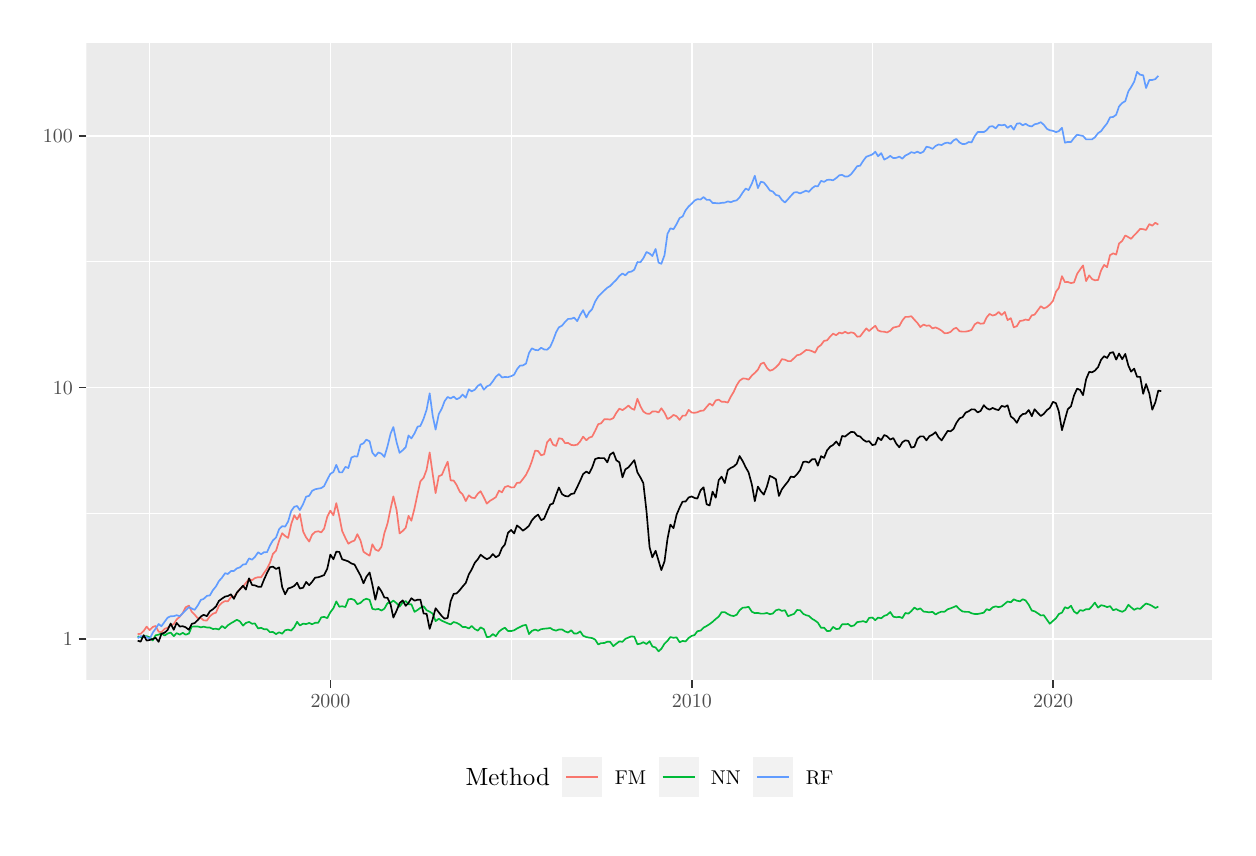
\begin{tikzpicture}[x=1pt,y=1pt]
\definecolor{fillColor}{RGB}{255,255,255}
\path[use as bounding box,fill=fillColor,fill opacity=0.00] (0,0) rectangle (433.62,289.08);
\begin{scope}
\path[clip] (  0.00,  0.00) rectangle (433.62,289.08);
\definecolor{drawColor}{RGB}{255,255,255}
\definecolor{fillColor}{RGB}{255,255,255}

\path[draw=drawColor,line width= 0.6pt,line join=round,line cap=round,fill=fillColor] (  0.00,  0.00) rectangle (433.62,289.08);
\end{scope}
\begin{scope}
\path[clip] ( 21.25, 53.26) rectangle (428.12,283.58);
\definecolor{fillColor}{gray}{0.92}

\path[fill=fillColor] ( 21.25, 53.26) rectangle (428.12,283.58);
\definecolor{drawColor}{RGB}{255,255,255}

\path[draw=drawColor,line width= 0.3pt,line join=round] ( 21.25,113.62) --
	(428.12,113.62);

\path[draw=drawColor,line width= 0.3pt,line join=round] ( 21.25,204.56) --
	(428.12,204.56);

\path[draw=drawColor,line width= 0.3pt,line join=round] ( 44.12, 53.26) --
	( 44.12,283.58);

\path[draw=drawColor,line width= 0.3pt,line join=round] (174.69, 53.26) --
	(174.69,283.58);

\path[draw=drawColor,line width= 0.3pt,line join=round] (305.25, 53.26) --
	(305.25,283.58);

\path[draw=drawColor,line width= 0.6pt,line join=round] ( 21.25, 68.15) --
	(428.12, 68.15);

\path[draw=drawColor,line width= 0.6pt,line join=round] ( 21.25,159.09) --
	(428.12,159.09);

\path[draw=drawColor,line width= 0.6pt,line join=round] ( 21.25,250.03) --
	(428.12,250.03);

\path[draw=drawColor,line width= 0.6pt,line join=round] (109.41, 53.26) --
	(109.41,283.58);

\path[draw=drawColor,line width= 0.6pt,line join=round] (239.98, 53.26) --
	(239.98,283.58);

\path[draw=drawColor,line width= 0.6pt,line join=round] (370.52, 53.26) --
	(370.52,283.58);
\definecolor{drawColor}{RGB}{248,118,109}

\path[draw=drawColor,line width= 0.6pt,line join=round] ( 39.74, 69.95) --
	( 40.81, 70.05) --
	( 41.92, 71.09) --
	( 42.99, 72.64) --
	( 44.07, 71.36) --
	( 45.21, 72.53) --
	( 46.21, 72.87) --
	( 47.32, 70.85) --
	( 48.32, 70.61) --
	( 49.50, 71.87) --
	( 50.57, 72.20) --
	( 51.68, 73.15) --
	( 52.79, 73.55) --
	( 53.82, 75.22) --
	( 54.97, 76.25) --
	( 56.04, 77.56) --
	( 57.08, 79.63) --
	( 58.26, 80.23) --
	( 59.29, 78.02) --
	( 60.33, 77.00) --
	( 61.47, 75.62) --
	( 62.58, 75.79) --
	( 63.58, 74.91) --
	( 64.76, 74.86) --
	( 65.84, 76.37) --
	( 66.94, 77.31) --
	( 68.05, 77.69) --
	( 69.09, 80.16) --
	( 70.23, 81.28) --
	( 71.34, 81.89) --
	( 72.34, 81.77) --
	( 73.45, 83.32) --
	( 74.52, 83.38) --
	( 75.59, 84.78) --
	( 76.70, 86.17) --
	( 77.81, 87.13) --
	( 78.85, 88.44) --
	( 79.99, 89.81) --
	( 81.10, 89.43) --
	( 82.10, 90.18) --
	( 83.28, 90.52) --
	( 84.35, 90.47) --
	( 85.35, 91.97) --
	( 86.50, 93.59) --
	( 87.57, 95.73) --
	( 88.60, 98.89) --
	( 89.75,100.08) --
	( 90.86,103.67) --
	( 91.96,106.40) --
	( 93.04,105.39) --
	( 94.11,104.68) --
	( 95.22,109.65) --
	( 96.33,112.90) --
	( 97.36,111.38) --
	( 98.36,113.33) --
	( 99.54,107.02) --
	(100.61,104.90) --
	(101.72,103.38) --
	(102.79,105.88) --
	(103.87,106.87) --
	(105.01,107.11) --
	(106.08,106.70) --
	(107.12,108.05) --
	(108.26,112.34) --
	(109.37,114.56) --
	(110.48,112.86) --
	(111.52,117.26) --
	(112.62,112.42) --
	(113.63,107.22) --
	(114.81,104.67) --
	(115.88,102.60) --
	(116.99,103.33) --
	(118.09,103.75) --
	(119.13,106.05) --
	(120.27,103.75) --
	(121.35, 99.71) --
	(122.38, 98.99) --
	(123.56, 98.27) --
	(124.56,102.39) --
	(125.64,100.51) --
	(126.74, 99.97) --
	(127.85,101.51) --
	(128.89,106.41) --
	(130.03,109.91) --
	(131.14,115.27) --
	(132.14,119.69) --
	(133.32,114.73) --
	(134.39,106.33) --
	(135.50,107.20) --
	(136.61,108.36) --
	(137.61,112.67) --
	(138.65,110.90) --
	(139.79,115.43) --
	(140.90,120.69) --
	(141.90,125.13) --
	(143.08,126.46) --
	(144.15,129.35) --
	(145.26,135.59) --
	(146.37,127.69) --
	(147.40,120.89) --
	(148.55,126.99) --
	(149.66,127.46) --
	(150.66,129.81) --
	(151.76,132.25) --
	(152.84,125.48) --
	(153.91,125.44) --
	(155.02,123.77) --
	(156.13,121.42) --
	(157.16,120.44) --
	(158.31,118.02) --
	(159.41,120.10) --
	(160.42,119.24) --
	(161.59,119.11) --
	(162.67,120.71) --
	(163.67,121.57) --
	(164.85,119.29) --
	(165.92,117.09) --
	(167.03,118.10) --
	(168.10,118.72) --
	(169.17,119.42) --
	(170.32,121.77) --
	(171.39,121.17) --
	(172.43,123.10) --
	(173.57,123.47) --
	(174.68,122.94) --
	(175.79,122.98) --
	(176.79,124.60) --
	(177.89,124.63) --
	(178.93,125.95) --
	(180.07,127.49) --
	(181.15,129.67) --
	(182.18,132.37) --
	(183.36,136.24) --
	(184.44,136.10) --
	(185.54,134.57) --
	(186.62,134.90) --
	(187.69,139.25) --
	(188.83,140.53) --
	(189.83,138.41) --
	(190.94,137.94) --
	(191.94,140.72) --
	(193.12,140.49) --
	(194.19,138.94) --
	(195.30,139.01) --
	(196.41,138.30) --
	(197.45,138.18) --
	(198.59,138.40) --
	(199.66,139.58) --
	(200.70,141.29) --
	(201.88,140.00) --
	(202.88,140.92) --
	(203.95,141.30) --
	(205.06,143.41) --
	(206.17,145.80) --
	(207.20,146.10) --
	(208.35,147.56) --
	(209.46,147.60) --
	(210.46,147.46) --
	(211.64,148.01) --
	(212.71,149.91) --
	(213.82,151.41) --
	(214.93,150.88) --
	(215.96,151.59) --
	(217.07,152.52) --
	(218.14,151.50) --
	(219.21,151.00) --
	(220.32,154.99) --
	(221.43,152.24) --
	(222.47,150.36) --
	(223.61,149.63) --
	(224.72,149.51) --
	(225.72,150.38) --
	(226.90,150.43) --
	(227.97,150.04) --
	(228.97,151.55) --
	(230.12,149.94) --
	(231.19,147.68) --
	(232.23,148.16) --
	(233.37,149.14) --
	(234.48,148.68) --
	(235.59,147.33) --
	(236.66,148.89) --
	(237.73,148.89) --
	(238.84,150.97) --
	(239.95,150.00) --
	(240.98,149.90) --
	(241.98,150.12) --
	(243.16,150.63) --
	(244.24,150.73) --
	(245.34,152.04) --
	(246.42,153.27) --
	(247.49,152.53) --
	(248.63,154.39) --
	(249.70,154.67) --
	(250.74,153.91) --
	(251.89,153.88) --
	(252.99,153.62) --
	(254.10,155.79) --
	(255.10,157.46) --
	(256.21,159.87) --
	(257.25,161.50) --
	(258.39,162.30) --
	(259.46,162.26) --
	(260.50,161.89) --
	(261.68,163.38) --
	(262.75,164.33) --
	(263.86,165.49) --
	(264.93,167.58) --
	(266.00,168.06) --
	(267.15,166.11) --
	(268.18,165.11) --
	(269.26,165.49) --
	(270.37,166.36) --
	(271.47,167.50) --
	(272.51,169.30) --
	(273.65,169.10) --
	(274.76,168.59) --
	(275.76,168.58) --
	(276.94,169.66) --
	(278.01,170.71) --
	(279.12,170.96) --
	(280.23,171.77) --
	(281.23,172.58) --
	(282.27,172.57) --
	(283.41,172.19) --
	(284.52,171.63) --
	(285.52,173.54) --
	(286.70,174.47) --
	(287.77,175.90) --
	(288.88,176.11) --
	(289.99,177.48) --
	(291.03,178.53) --
	(292.17,177.95) --
	(293.28,178.91) --
	(294.28,178.58) --
	(295.39,179.21) --
	(296.46,178.59) --
	(297.53,179.00) --
	(298.64,178.69) --
	(299.75,177.41) --
	(300.78,177.49) --
	(301.93,179.01) --
	(303.04,180.41) --
	(304.04,179.46) --
	(305.22,180.51) --
	(306.29,181.35) --
	(307.29,179.67) --
	(308.43,179.27) --
	(309.51,179.21) --
	(310.54,178.94) --
	(311.69,179.58) --
	(312.79,180.71) --
	(313.90,180.96) --
	(314.97,181.26) --
	(316.05,183.26) --
	(317.15,184.59) --
	(318.26,184.58) --
	(319.30,184.82) --
	(320.41,183.54) --
	(321.52,182.36) --
	(322.55,180.88) --
	(323.70,181.79) --
	(324.77,181.36) --
	(325.80,181.49) --
	(326.98,180.40) --
	(328.06,180.76) --
	(329.16,180.27) --
	(330.24,179.60) --
	(331.31,178.67) --
	(332.45,178.73) --
	(333.45,179.13) --
	(334.56,180.21) --
	(335.56,180.65) --
	(336.74,179.37) --
	(337.82,179.24) --
	(338.92,179.26) --
	(340.03,179.47) --
	(341.07,179.87) --
	(342.21,181.86) --
	(343.28,182.58) --
	(344.32,182.10) --
	(345.50,182.22) --
	(346.50,184.36) --
	(347.57,185.63) --
	(348.68,185.07) --
	(349.79,185.37) --
	(350.83,186.36) --
	(351.97,185.23) --
	(353.08,186.34) --
	(354.08,183.43) --
	(355.26,184.09) --
	(356.33,180.80) --
	(357.44,181.23) --
	(358.55,183.08) --
	(359.55,183.24) --
	(360.58,183.61) --
	(361.73,183.38) --
	(362.84,185.13) --
	(363.84,185.37) --
	(365.02,186.98) --
	(366.09,188.43) --
	(367.20,187.61) --
	(368.31,188.14) --
	(369.34,188.99) --
	(370.49,190.35) --
	(371.59,193.69) --
	(372.59,195.01) --
	(373.74,199.29) --
	(374.81,197.12) --
	(375.85,197.19) --
	(376.99,196.77) --
	(378.10,197.02) --
	(379.21,200.10) --
	(380.28,201.68) --
	(381.35,203.16) --
	(382.46,197.50) --
	(383.57,199.56) --
	(384.60,198.25) --
	(385.61,197.80) --
	(386.79,197.92) --
	(387.86,201.34) --
	(388.97,203.35) --
	(390.04,202.54) --
	(391.11,206.90) --
	(392.25,207.51) --
	(393.33,207.10) --
	(394.36,211.08) --
	(395.51,212.04) --
	(396.61,213.99) --
	(397.72,213.39) --
	(398.72,212.78) --
	(399.83,214.07) --
	(400.87,215.11) --
	(402.01,216.38) --
	(403.08,216.27) --
	(404.12,215.98) --
	(405.30,218.10) --
	(406.37,217.51) --
	(407.48,218.58) --
	(408.55,217.92);
\definecolor{drawColor}{RGB}{0,186,56}

\path[draw=drawColor,line width= 0.6pt,line join=round] ( 39.74, 69.16) --
	( 40.81, 68.73) --
	( 41.92, 69.15) --
	( 42.99, 69.18) --
	( 44.07, 68.80) --
	( 45.21, 67.65) --
	( 46.21, 69.51) --
	( 47.32, 69.75) --
	( 48.32, 70.17) --
	( 49.50, 69.43) --
	( 50.57, 70.15) --
	( 51.68, 70.50) --
	( 52.79, 69.21) --
	( 53.82, 70.29) --
	( 54.97, 69.76) --
	( 56.04, 70.40) --
	( 57.08, 69.73) --
	( 58.26, 70.15) --
	( 59.29, 72.64) --
	( 60.33, 72.68) --
	( 61.47, 72.69) --
	( 62.58, 72.40) --
	( 63.58, 72.63) --
	( 64.76, 72.34) --
	( 65.84, 72.32) --
	( 66.94, 71.79) --
	( 68.05, 71.88) --
	( 69.09, 71.62) --
	( 70.23, 72.87) --
	( 71.34, 72.08) --
	( 72.34, 73.14) --
	( 73.45, 73.87) --
	( 74.52, 74.47) --
	( 75.59, 75.12) --
	( 76.70, 74.53) --
	( 77.81, 73.01) --
	( 78.85, 73.97) --
	( 79.99, 74.37) --
	( 81.10, 73.68) --
	( 82.10, 73.81) --
	( 83.28, 71.98) --
	( 84.35, 72.23) --
	( 85.35, 71.72) --
	( 86.50, 71.67) --
	( 87.57, 70.64) --
	( 88.60, 70.72) --
	( 89.75, 69.96) --
	( 90.86, 70.61) --
	( 91.96, 70.08) --
	( 93.04, 71.34) --
	( 94.11, 71.56) --
	( 95.22, 71.22) --
	( 96.33, 72.45) --
	( 97.36, 74.39) --
	( 98.36, 73.06) --
	( 99.54, 73.74) --
	(100.61, 73.56) --
	(101.72, 73.97) --
	(102.79, 73.51) --
	(103.87, 74.04) --
	(105.01, 74.06) --
	(106.08, 75.99) --
	(107.12, 76.18) --
	(108.26, 75.71) --
	(109.37, 77.85) --
	(110.48, 79.31) --
	(111.52, 81.76) --
	(112.62, 79.82) --
	(113.63, 80.02) --
	(114.81, 79.73) --
	(115.88, 82.50) --
	(116.99, 82.67) --
	(118.09, 82.24) --
	(119.13, 80.77) --
	(120.27, 81.23) --
	(121.35, 82.27) --
	(122.38, 82.72) --
	(123.56, 82.30) --
	(124.56, 79.06) --
	(125.64, 78.84) --
	(126.74, 79.03) --
	(127.85, 78.46) --
	(128.89, 79.13) --
	(130.03, 81.16) --
	(131.14, 81.30) --
	(132.14, 82.05) --
	(133.32, 81.10) --
	(134.39, 79.87) --
	(135.50, 81.32) --
	(136.61, 81.88) --
	(137.61, 80.76) --
	(138.65, 80.72) --
	(139.79, 77.99) --
	(140.90, 78.68) --
	(141.90, 79.44) --
	(143.08, 79.99) --
	(144.15, 78.56) --
	(145.26, 78.05) --
	(146.37, 77.31) --
	(147.40, 74.63) --
	(148.55, 75.49) --
	(149.66, 74.77) --
	(150.66, 74.34) --
	(151.76, 73.84) --
	(152.84, 73.46) --
	(153.91, 74.31) --
	(155.02, 74.00) --
	(156.13, 73.42) --
	(157.16, 72.51) --
	(158.31, 72.50) --
	(159.41, 71.97) --
	(160.42, 72.88) --
	(161.59, 71.75) --
	(162.67, 71.20) --
	(163.67, 72.39) --
	(164.85, 71.72) --
	(165.92, 68.84) --
	(167.03, 68.99) --
	(168.10, 69.95) --
	(169.17, 69.19) --
	(170.32, 70.87) --
	(171.39, 71.68) --
	(172.43, 72.26) --
	(173.57, 71.06) --
	(174.68, 71.04) --
	(175.79, 71.33) --
	(176.79, 71.95) --
	(177.89, 72.50) --
	(178.93, 73.03) --
	(180.07, 73.30) --
	(181.15, 69.95) --
	(182.18, 71.09) --
	(183.36, 71.58) --
	(184.44, 71.15) --
	(185.54, 71.72) --
	(186.62, 71.89) --
	(187.69, 71.99) --
	(188.83, 72.15) --
	(189.83, 71.52) --
	(190.94, 71.20) --
	(191.94, 71.60) --
	(193.12, 71.62) --
	(194.19, 70.91) --
	(195.30, 70.52) --
	(196.41, 71.35) --
	(197.45, 70.13) --
	(198.59, 70.20) --
	(199.66, 70.92) --
	(200.70, 69.36) --
	(201.88, 68.86) --
	(202.88, 68.69) --
	(203.95, 68.51) --
	(205.06, 67.97) --
	(206.17, 66.19) --
	(207.20, 66.68) --
	(208.35, 66.72) --
	(209.46, 67.20) --
	(210.46, 67.14) --
	(211.64, 65.61) --
	(212.71, 66.49) --
	(213.82, 67.33) --
	(214.93, 67.15) --
	(215.96, 68.23) --
	(217.07, 68.69) --
	(218.14, 69.13) --
	(219.21, 69.00) --
	(220.32, 66.28) --
	(221.43, 66.51) --
	(222.47, 67.01) --
	(223.61, 66.35) --
	(224.72, 67.37) --
	(225.72, 65.50) --
	(226.90, 65.10) --
	(227.97, 63.73) --
	(228.97, 64.61) --
	(230.12, 66.49) --
	(231.19, 67.50) --
	(232.23, 68.88) --
	(233.37, 68.61) --
	(234.48, 68.77) --
	(235.59, 66.99) --
	(236.66, 67.49) --
	(237.73, 67.29) --
	(238.84, 68.57) --
	(239.95, 69.30) --
	(240.98, 69.61) --
	(241.98, 70.97) --
	(243.16, 71.22) --
	(244.24, 72.28) --
	(245.34, 72.88) --
	(246.42, 73.56) --
	(247.49, 74.38) --
	(248.63, 75.41) --
	(249.70, 76.25) --
	(250.74, 77.85) --
	(251.89, 77.89) --
	(252.99, 77.19) --
	(254.10, 76.65) --
	(255.10, 76.48) --
	(256.21, 76.95) --
	(257.25, 78.56) --
	(258.39, 79.50) --
	(259.46, 79.55) --
	(260.50, 79.81) --
	(261.68, 78.02) --
	(262.75, 77.53) --
	(263.86, 77.59) --
	(264.93, 77.34) --
	(266.00, 77.36) --
	(267.15, 77.58) --
	(268.18, 77.14) --
	(269.26, 77.38) --
	(270.37, 78.55) --
	(271.47, 78.87) --
	(272.51, 78.34) --
	(273.65, 78.55) --
	(274.76, 76.40) --
	(275.76, 76.82) --
	(276.94, 77.26) --
	(278.01, 78.65) --
	(279.12, 78.58) --
	(280.23, 77.28) --
	(281.23, 76.79) --
	(282.27, 76.53) --
	(283.41, 75.49) --
	(284.52, 74.85) --
	(285.52, 74.10) --
	(286.70, 72.20) --
	(287.77, 72.28) --
	(288.88, 71.02) --
	(289.99, 71.13) --
	(291.03, 72.54) --
	(292.17, 71.76) --
	(293.28, 71.90) --
	(294.28, 73.49) --
	(295.39, 73.48) --
	(296.46, 73.60) --
	(297.53, 72.77) --
	(298.64, 73.08) --
	(299.75, 74.28) --
	(300.78, 74.42) --
	(301.93, 74.63) --
	(303.04, 74.19) --
	(304.04, 75.78) --
	(305.22, 75.94) --
	(306.29, 74.98) --
	(307.29, 75.92) --
	(308.43, 75.66) --
	(309.51, 76.55) --
	(310.54, 76.90) --
	(311.69, 77.92) --
	(312.79, 76.24) --
	(313.90, 76.03) --
	(314.97, 76.17) --
	(316.05, 75.74) --
	(317.15, 77.57) --
	(318.26, 77.35) --
	(319.30, 78.25) --
	(320.41, 79.52) --
	(321.52, 78.81) --
	(322.55, 79.24) --
	(323.70, 78.09) --
	(324.77, 77.97) --
	(325.80, 77.81) --
	(326.98, 77.99) --
	(328.06, 77.02) --
	(329.16, 77.68) --
	(330.24, 78.06) --
	(331.31, 78.03) --
	(332.45, 78.92) --
	(333.45, 79.25) --
	(334.56, 79.69) --
	(335.56, 80.12) --
	(336.74, 78.90) --
	(337.82, 78.11) --
	(338.92, 77.99) --
	(340.03, 77.97) --
	(341.07, 77.46) --
	(342.21, 77.22) --
	(343.28, 77.22) --
	(344.32, 77.42) --
	(345.50, 77.69) --
	(346.50, 78.95) --
	(347.57, 78.56) --
	(348.68, 79.62) --
	(349.79, 79.97) --
	(350.83, 79.70) --
	(351.97, 79.96) --
	(353.08, 80.90) --
	(354.08, 81.72) --
	(355.26, 81.45) --
	(356.33, 82.51) --
	(357.44, 82.02) --
	(358.55, 81.79) --
	(359.55, 82.54) --
	(360.58, 82.13) --
	(361.73, 80.55) --
	(362.84, 78.42) --
	(363.84, 78.21) --
	(365.02, 77.45) --
	(366.09, 76.69) --
	(367.20, 76.76) --
	(368.31, 75.13) --
	(369.34, 73.69) --
	(370.49, 74.73) --
	(371.59, 75.69) --
	(372.59, 77.18) --
	(373.74, 77.71) --
	(374.81, 79.65) --
	(375.85, 79.23) --
	(376.99, 80.18) --
	(378.10, 78.09) --
	(379.21, 77.33) --
	(380.28, 78.63) --
	(381.35, 78.37) --
	(382.46, 78.93) --
	(383.57, 78.92) --
	(384.60, 80.01) --
	(385.61, 81.33) --
	(386.79, 79.50) --
	(387.86, 80.37) --
	(388.97, 80.16) --
	(390.04, 79.70) --
	(391.11, 80.06) --
	(392.25, 78.58) --
	(393.33, 78.97) --
	(394.36, 78.43) --
	(395.51, 78.01) --
	(396.61, 78.63) --
	(397.72, 80.54) --
	(398.72, 79.63) --
	(399.83, 78.71) --
	(400.87, 79.27) --
	(402.01, 79.06) --
	(403.08, 80.13) --
	(404.12, 81.01) --
	(405.30, 80.62) --
	(406.37, 80.08) --
	(407.48, 79.37) --
	(408.55, 79.89);
\definecolor{drawColor}{RGB}{97,156,255}

\path[draw=drawColor,line width= 0.6pt,line join=round] ( 39.74, 68.47) --
	( 40.81, 69.19) --
	( 41.92, 69.08) --
	( 42.99, 68.85) --
	( 44.07, 68.23) --
	( 45.21, 70.49) --
	( 46.21, 71.88) --
	( 47.32, 73.58) --
	( 48.32, 72.79) --
	( 49.50, 74.42) --
	( 50.57, 75.89) --
	( 51.68, 76.40) --
	( 52.79, 76.44) --
	( 53.82, 76.77) --
	( 54.97, 76.43) --
	( 56.04, 77.49) --
	( 57.08, 78.52) --
	( 58.26, 79.71) --
	( 59.29, 79.20) --
	( 60.33, 78.71) --
	( 61.47, 80.30) --
	( 62.58, 82.31) --
	( 63.58, 82.66) --
	( 64.76, 83.76) --
	( 65.84, 83.93) --
	( 66.94, 85.84) --
	( 68.05, 87.19) --
	( 69.09, 89.08) --
	( 70.23, 90.35) --
	( 71.34, 91.96) --
	( 72.34, 91.66) --
	( 73.45, 92.73) --
	( 74.52, 92.77) --
	( 75.59, 93.68) --
	( 76.70, 94.06) --
	( 77.81, 95.07) --
	( 78.85, 95.23) --
	( 79.99, 97.30) --
	( 81.10, 96.84) --
	( 82.10, 97.82) --
	( 83.28, 99.52) --
	( 84.35, 98.78) --
	( 85.35, 99.51) --
	( 86.50, 99.57) --
	( 87.57,101.99) --
	( 88.60,103.78) --
	( 89.75,104.86) --
	( 90.86,107.87) --
	( 91.96,108.94) --
	( 93.04,108.79) --
	( 94.11,110.62) --
	( 95.22,114.42) --
	( 96.33,115.95) --
	( 97.36,116.24) --
	( 98.36,114.75) --
	( 99.54,116.96) --
	(100.61,119.60) --
	(101.72,119.92) --
	(102.79,121.72) --
	(103.87,122.29) --
	(105.01,122.52) --
	(106.08,122.71) --
	(107.12,123.41) --
	(108.26,125.76) --
	(109.37,127.85) --
	(110.48,128.54) --
	(111.52,131.10) --
	(112.62,128.37) --
	(113.63,128.38) --
	(114.81,130.38) --
	(115.88,129.95) --
	(116.99,133.76) --
	(118.09,134.21) --
	(119.13,134.10) --
	(120.27,138.40) --
	(121.35,138.91) --
	(122.38,140.21) --
	(123.56,139.59) --
	(124.56,135.50) --
	(125.64,134.22) --
	(126.74,135.60) --
	(127.85,135.13) --
	(128.89,133.96) --
	(130.03,137.83) --
	(131.14,142.40) --
	(132.14,144.76) --
	(133.32,139.22) --
	(134.39,135.45) --
	(135.50,136.37) --
	(136.61,137.50) --
	(137.61,141.72) --
	(138.65,140.65) --
	(139.79,142.48) --
	(140.90,144.90) --
	(141.90,145.15) --
	(143.08,147.79) --
	(144.15,150.99) --
	(145.26,156.95) --
	(146.37,148.75) --
	(147.40,143.86) --
	(148.55,149.44) --
	(149.66,151.48) --
	(150.66,154.13) --
	(151.76,155.64) --
	(152.84,155.11) --
	(153.91,155.78) --
	(155.02,154.81) --
	(156.13,155.35) --
	(157.16,156.51) --
	(158.31,155.37) --
	(159.41,158.39) --
	(160.42,157.66) --
	(161.59,158.27) --
	(162.67,159.66) --
	(163.67,160.30) --
	(164.85,158.26) --
	(165.92,159.42) --
	(167.03,159.96) --
	(168.10,161.31) --
	(169.17,162.94) --
	(170.32,163.90) --
	(171.39,162.68) --
	(172.43,162.86) --
	(173.57,162.79) --
	(174.68,163.14) --
	(175.79,163.68) --
	(176.79,165.61) --
	(177.89,166.96) --
	(178.93,167.03) --
	(180.07,167.71) --
	(181.15,171.50) --
	(182.18,173.22) --
	(183.36,172.64) --
	(184.44,172.51) --
	(185.54,173.42) --
	(186.62,172.79) --
	(187.69,172.71) --
	(188.83,173.79) --
	(189.83,176.02) --
	(190.94,178.99) --
	(191.94,180.79) --
	(193.12,181.43) --
	(194.19,182.78) --
	(195.30,183.84) --
	(196.41,183.89) --
	(197.45,184.30) --
	(198.59,183.03) --
	(199.66,185.31) --
	(200.70,187.00) --
	(201.88,184.37) --
	(202.88,186.24) --
	(203.95,187.34) --
	(205.06,190.11) --
	(206.17,191.92) --
	(207.20,192.94) --
	(208.35,194.10) --
	(209.46,195.12) --
	(210.46,195.71) --
	(211.64,196.93) --
	(212.71,197.98) --
	(213.82,199.37) --
	(214.93,200.26) --
	(215.96,199.57) --
	(217.07,200.74) --
	(218.14,200.93) --
	(219.21,201.65) --
	(220.32,204.38) --
	(221.43,204.33) --
	(222.47,205.77) --
	(223.61,208.03) --
	(224.72,207.48) --
	(225.72,206.55) --
	(226.90,209.11) --
	(227.97,204.21) --
	(228.97,203.75) --
	(230.12,206.87) --
	(231.19,214.56) --
	(232.23,216.56) --
	(233.37,216.25) --
	(234.48,218.10) --
	(235.59,220.30) --
	(236.66,220.85) --
	(237.73,223.06) --
	(238.84,224.49) --
	(239.95,225.49) --
	(240.98,226.60) --
	(241.98,227.09) --
	(243.16,227.00) --
	(244.24,227.87) --
	(245.34,226.84) --
	(246.42,226.88) --
	(247.49,225.74) --
	(248.63,225.69) --
	(249.70,225.58) --
	(250.74,225.77) --
	(251.89,225.85) --
	(252.99,226.29) --
	(254.10,226.01) --
	(255.10,226.45) --
	(256.21,226.68) --
	(257.25,227.75) --
	(258.39,229.53) --
	(259.46,230.95) --
	(260.50,230.41) --
	(261.68,232.76) --
	(262.75,235.57) --
	(263.86,231.09) --
	(264.93,233.40) --
	(266.00,233.14) --
	(267.15,231.72) --
	(268.18,230.25) --
	(269.26,229.86) --
	(270.37,228.62) --
	(271.47,228.34) --
	(272.51,226.87) --
	(273.65,225.90) --
	(274.76,227.12) --
	(275.76,228.29) --
	(276.94,229.53) --
	(278.01,229.64) --
	(279.12,229.17) --
	(280.23,229.71) --
	(281.23,230.17) --
	(282.27,229.75) --
	(283.41,231.02) --
	(284.52,231.85) --
	(285.52,231.73) --
	(286.70,233.74) --
	(287.77,233.36) --
	(288.88,234.08) --
	(289.99,234.12) --
	(291.03,233.94) --
	(292.17,234.73) --
	(293.28,235.72) --
	(294.28,235.90) --
	(295.39,235.26) --
	(296.46,235.34) --
	(297.53,236.11) --
	(298.64,237.54) --
	(299.75,239.04) --
	(300.78,239.19) --
	(301.93,240.99) --
	(303.04,242.44) --
	(304.04,242.80) --
	(305.22,243.27) --
	(306.29,244.24) --
	(307.29,242.62) --
	(308.43,243.74) --
	(309.51,241.41) --
	(310.54,241.93) --
	(311.69,242.74) --
	(312.79,241.94) --
	(313.90,242.04) --
	(314.97,242.49) --
	(316.05,241.74) --
	(317.15,242.89) --
	(318.26,243.40) --
	(319.30,244.08) --
	(320.41,243.80) --
	(321.52,244.26) --
	(322.55,243.72) --
	(323.70,244.28) --
	(324.77,246.06) --
	(325.80,245.83) --
	(326.98,245.29) --
	(328.06,246.33) --
	(329.16,246.88) --
	(330.24,246.66) --
	(331.31,247.31) --
	(332.45,247.56) --
	(333.45,247.14) --
	(334.56,248.34) --
	(335.56,248.87) --
	(336.74,247.59) --
	(337.82,247.00) --
	(338.92,247.10) --
	(340.03,247.75) --
	(341.07,247.61) --
	(342.21,249.89) --
	(343.28,251.35) --
	(344.32,251.38) --
	(345.50,251.35) --
	(346.50,252.02) --
	(347.57,253.31) --
	(348.68,253.49) --
	(349.79,252.69) --
	(350.83,253.99) --
	(351.97,253.80) --
	(353.08,254.01) --
	(354.08,252.87) --
	(355.26,253.68) --
	(356.33,252.24) --
	(357.44,254.39) --
	(358.55,254.53) --
	(359.55,253.80) --
	(360.58,254.35) --
	(361.73,253.61) --
	(362.84,253.38) --
	(363.84,254.17) --
	(365.02,254.42) --
	(366.09,254.92) --
	(367.20,253.95) --
	(368.31,252.53) --
	(369.34,252.01) --
	(370.49,251.79) --
	(371.59,251.33) --
	(372.59,251.68) --
	(373.74,252.88) --
	(374.81,247.51) --
	(375.85,247.79) --
	(376.99,247.74) --
	(378.10,249.24) --
	(379.21,250.39) --
	(380.28,250.16) --
	(381.35,249.93) --
	(382.46,248.73) --
	(383.57,248.71) --
	(384.60,248.73) --
	(385.61,249.43) --
	(386.79,250.96) --
	(387.86,251.67) --
	(388.97,253.19) --
	(390.04,254.49) --
	(391.11,256.69) --
	(392.25,256.82) --
	(393.33,257.63) --
	(394.36,260.61) --
	(395.51,261.88) --
	(396.61,262.52) --
	(397.72,266.06) --
	(398.72,267.60) --
	(399.83,269.56) --
	(400.87,273.11) --
	(402.01,272.05) --
	(403.08,271.91) --
	(404.12,267.26) --
	(405.30,270.15) --
	(406.37,270.18) --
	(407.48,270.49) --
	(408.55,271.68);
\definecolor{drawColor}{RGB}{0,0,0}

\path[draw=drawColor,line width= 0.6pt,line join=round] ( 39.74, 67.60) --
	( 40.81, 67.20) --
	( 41.92, 69.54) --
	( 42.99, 67.61) --
	( 44.07, 67.82) --
	( 45.21, 68.15) --
	( 46.21, 68.62) --
	( 47.32, 67.14) --
	( 48.32, 70.04) --
	( 49.50, 70.45) --
	( 50.57, 71.46) --
	( 51.68, 73.77) --
	( 52.79, 71.50) --
	( 53.82, 73.98) --
	( 54.97, 72.69) --
	( 56.04, 72.79) --
	( 57.08, 72.42) --
	( 58.26, 71.50) --
	( 59.29, 73.65) --
	( 60.33, 73.94) --
	( 61.47, 75.02) --
	( 62.58, 76.30) --
	( 63.58, 76.92) --
	( 64.76, 76.43) --
	( 65.84, 78.18) --
	( 66.94, 78.92) --
	( 68.05, 79.94) --
	( 69.09, 81.91) --
	( 70.23, 82.77) --
	( 71.34, 83.52) --
	( 72.34, 83.70) --
	( 73.45, 84.33) --
	( 74.52, 82.68) --
	( 75.59, 84.94) --
	( 76.70, 86.16) --
	( 77.81, 87.43) --
	( 78.85, 86.02) --
	( 79.99, 90.09) --
	( 81.10, 87.68) --
	( 82.10, 87.56) --
	( 83.28, 87.06) --
	( 84.35, 87.00) --
	( 85.35, 89.52) --
	( 86.50, 92.06) --
	( 87.57, 94.12) --
	( 88.60, 94.33) --
	( 89.75, 93.47) --
	( 90.86, 94.03) --
	( 91.96, 86.92) --
	( 93.04, 84.33) --
	( 94.11, 86.43) --
	( 95.22, 86.78) --
	( 96.33, 87.36) --
	( 97.36, 88.49) --
	( 98.36, 86.41) --
	( 99.54, 86.70) --
	(100.61, 88.79) --
	(101.72, 87.62) --
	(102.79, 88.84) --
	(103.87, 90.35) --
	(105.01, 90.48) --
	(106.08, 90.86) --
	(107.12, 91.28) --
	(108.26, 93.59) --
	(109.37, 98.68) --
	(110.48, 97.01) --
	(111.52, 99.73) --
	(112.62, 99.63) --
	(113.63, 96.98) --
	(114.81, 96.60) --
	(115.88, 96.21) --
	(116.99, 95.45) --
	(118.09, 95.11) --
	(119.13, 93.19) --
	(120.27, 91.09) --
	(121.35, 88.30) --
	(122.38, 90.63) --
	(123.56, 92.19) --
	(124.56, 87.81) --
	(125.64, 82.38) --
	(126.74, 87.01) --
	(127.85, 85.38) --
	(128.89, 83.15) --
	(130.03, 83.05) --
	(131.14, 80.65) --
	(132.14, 75.92) --
	(133.32, 78.45) --
	(134.39, 81.12) --
	(135.50, 82.13) --
	(136.61, 80.15) --
	(137.61, 81.21) --
	(138.65, 82.92) --
	(139.79, 82.02) --
	(140.90, 82.37) --
	(141.90, 82.40) --
	(143.08, 77.36) --
	(144.15, 77.30) --
	(145.26, 71.84) --
	(146.37, 75.46) --
	(147.40, 79.30) --
	(148.55, 77.83) --
	(149.66, 76.43) --
	(150.66, 75.51) --
	(151.76, 75.81) --
	(152.84, 81.82) --
	(153.91, 84.48) --
	(155.02, 84.65) --
	(156.13, 85.84) --
	(157.16, 87.12) --
	(158.31, 88.45) --
	(159.41, 91.52) --
	(160.42, 93.26) --
	(161.59, 95.76) --
	(162.67, 97.01) --
	(163.67, 98.62) --
	(164.85, 97.70) --
	(165.92, 97.01) --
	(167.03, 97.58) --
	(168.10, 98.87) --
	(169.17, 97.71) --
	(170.32, 98.42) --
	(171.39,101.05) --
	(172.43,102.31) --
	(173.57,106.56) --
	(174.68,107.56) --
	(175.79,106.32) --
	(176.79,109.21) --
	(177.89,108.38) --
	(178.93,107.32) --
	(180.07,108.11) --
	(181.15,109.09) --
	(182.18,111.03) --
	(183.36,112.37) --
	(184.44,113.11) --
	(185.54,111.13) --
	(186.62,111.67) --
	(187.69,114.21) --
	(188.83,116.76) --
	(189.83,117.15) --
	(190.94,120.28) --
	(191.94,122.91) --
	(193.12,120.50) --
	(194.19,119.86) --
	(195.30,119.68) --
	(196.41,120.59) --
	(197.45,120.76) --
	(198.59,123.12) --
	(199.66,125.40) --
	(200.70,127.77) --
	(201.88,128.70) --
	(202.88,128.01) --
	(203.95,130.07) --
	(205.06,133.21) --
	(206.17,133.57) --
	(207.20,133.53) --
	(208.35,133.52) --
	(209.46,132.01) --
	(210.46,134.83) --
	(211.64,135.60) --
	(212.71,132.77) --
	(213.82,132.01) --
	(214.93,126.59) --
	(215.96,129.46) --
	(217.07,130.19) --
	(218.14,131.47) --
	(219.21,132.82) --
	(220.32,128.40) --
	(221.43,126.53) --
	(222.47,124.45) --
	(223.61,114.32) --
	(224.72,101.39) --
	(225.72, 97.66) --
	(226.90,100.05) --
	(227.97, 96.45) --
	(228.97, 93.06) --
	(230.12, 96.23) --
	(231.19,104.32) --
	(232.23,109.48) --
	(233.37,108.24) --
	(234.48,113.08) --
	(235.59,115.69) --
	(236.66,117.82) --
	(237.73,117.85) --
	(238.84,119.31) --
	(239.95,119.70) --
	(240.98,119.14) --
	(241.98,118.92) --
	(243.16,121.91) --
	(244.24,122.99) --
	(245.34,116.85) --
	(246.42,116.42) --
	(247.49,121.43) --
	(248.63,119.22) --
	(249.70,125.58) --
	(250.74,126.81) --
	(251.89,124.51) --
	(252.99,129.20) --
	(254.10,130.02) --
	(255.10,130.46) --
	(256.21,131.49) --
	(257.25,134.28) --
	(258.39,132.41) --
	(259.46,130.20) --
	(260.50,128.39) --
	(261.68,124.00) --
	(262.75,117.98) --
	(263.86,123.25) --
	(264.93,121.57) --
	(266.00,120.34) --
	(267.15,123.34) --
	(268.18,127.11) --
	(269.26,126.60) --
	(270.37,125.91) --
	(271.47,119.85) --
	(272.51,122.24) --
	(273.65,123.75) --
	(274.76,125.12) --
	(275.76,126.88) --
	(276.94,126.65) --
	(278.01,127.74) --
	(279.12,129.21) --
	(280.23,132.15) --
	(281.23,132.29) --
	(282.27,131.91) --
	(283.41,133.10) --
	(284.52,133.19) --
	(285.52,130.80) --
	(286.70,134.23) --
	(287.77,133.61) --
	(288.88,136.37) --
	(289.99,137.69) --
	(291.03,138.29) --
	(292.17,139.54) --
	(293.28,138.06) --
	(294.28,141.53) --
	(295.39,141.34) --
	(296.46,142.22) --
	(297.53,143.02) --
	(298.64,142.91) --
	(299.75,141.61) --
	(300.78,141.37) --
	(301.93,140.16) --
	(303.04,139.47) --
	(304.04,139.67) --
	(305.22,138.25) --
	(306.29,138.49) --
	(307.29,140.93) --
	(308.43,140.02) --
	(309.51,141.89) --
	(310.54,141.42) --
	(311.69,140.24) --
	(312.79,140.78) --
	(313.90,138.70) --
	(314.97,137.45) --
	(316.05,139.27) --
	(317.15,139.97) --
	(318.26,139.73) --
	(319.30,137.34) --
	(320.41,137.62) --
	(321.52,140.50) --
	(322.55,141.40) --
	(323.70,141.39) --
	(324.77,139.96) --
	(325.80,141.43) --
	(326.98,142.04) --
	(328.06,142.92) --
	(329.16,141.04) --
	(330.24,139.93) --
	(331.31,141.60) --
	(332.45,143.39) --
	(333.45,143.22) --
	(334.56,144.06) --
	(335.56,146.23) --
	(336.74,147.92) --
	(337.82,148.33) --
	(338.92,149.99) --
	(340.03,150.46) --
	(341.07,151.17) --
	(342.21,151.12) --
	(343.28,150.07) --
	(344.32,150.55) --
	(345.50,152.65) --
	(346.50,151.59) --
	(347.57,151.07) --
	(348.68,151.66) --
	(349.79,151.17) --
	(350.83,150.89) --
	(351.97,152.41) --
	(353.08,152.06) --
	(354.08,152.60) --
	(355.26,148.59) --
	(356.33,147.76) --
	(357.44,146.28) --
	(358.55,148.54) --
	(359.55,149.45) --
	(360.58,149.59) --
	(361.73,150.91) --
	(362.84,148.68) --
	(363.84,151.21) --
	(365.02,149.84) --
	(366.09,148.76) --
	(367.20,149.55) --
	(368.31,150.90) --
	(369.34,151.65) --
	(370.49,153.88) --
	(371.59,153.35) --
	(372.59,150.43) --
	(373.74,143.64) --
	(374.81,147.53) --
	(375.85,151.23) --
	(376.99,152.26) --
	(378.10,156.21) --
	(379.21,158.64) --
	(380.28,158.18) --
	(381.35,156.27) --
	(382.46,162.05) --
	(383.57,164.69) --
	(384.60,164.55) --
	(385.61,165.12) --
	(386.79,166.44) --
	(387.86,169.05) --
	(388.97,170.38) --
	(390.04,169.72) --
	(391.11,171.54) --
	(392.25,171.82) --
	(393.33,169.13) --
	(394.36,171.32) --
	(395.51,169.28) --
	(396.61,171.18) --
	(397.72,167.00) --
	(398.72,164.78) --
	(399.83,165.87) --
	(400.87,162.92) --
	(402.01,162.90) --
	(403.08,156.79) --
	(404.12,160.29) --
	(405.30,156.87) --
	(406.37,151.04) --
	(407.48,153.70) --
	(408.55,157.93) --
	(409.63,157.74);
\end{scope}
\begin{scope}
\path[clip] (  0.00,  0.00) rectangle (433.62,289.08);
\definecolor{drawColor}{gray}{0.30}

\node[text=drawColor,anchor=base east,inner sep=0pt, outer sep=0pt, scale=  0.72] at ( 16.30, 65.67) {1};

\node[text=drawColor,anchor=base east,inner sep=0pt, outer sep=0pt, scale=  0.72] at ( 16.30,156.61) {10};

\node[text=drawColor,anchor=base east,inner sep=0pt, outer sep=0pt, scale=  0.72] at ( 16.30,247.55) {100};
\end{scope}
\begin{scope}
\path[clip] (  0.00,  0.00) rectangle (433.62,289.08);
\definecolor{drawColor}{gray}{0.20}

\path[draw=drawColor,line width= 0.6pt,line join=round] ( 18.50, 68.15) --
	( 21.25, 68.15);

\path[draw=drawColor,line width= 0.6pt,line join=round] ( 18.50,159.09) --
	( 21.25,159.09);

\path[draw=drawColor,line width= 0.6pt,line join=round] ( 18.50,250.03) --
	( 21.25,250.03);
\end{scope}
\begin{scope}
\path[clip] (  0.00,  0.00) rectangle (433.62,289.08);
\definecolor{drawColor}{gray}{0.20}

\path[draw=drawColor,line width= 0.6pt,line join=round] (109.41, 50.51) --
	(109.41, 53.26);

\path[draw=drawColor,line width= 0.6pt,line join=round] (239.98, 50.51) --
	(239.98, 53.26);

\path[draw=drawColor,line width= 0.6pt,line join=round] (370.52, 50.51) --
	(370.52, 53.26);
\end{scope}
\begin{scope}
\path[clip] (  0.00,  0.00) rectangle (433.62,289.08);
\definecolor{drawColor}{gray}{0.30}

\node[text=drawColor,anchor=base,inner sep=0pt, outer sep=0pt, scale=  0.72] at (109.41, 43.35) {2000};

\node[text=drawColor,anchor=base,inner sep=0pt, outer sep=0pt, scale=  0.72] at (239.98, 43.35) {2010};

\node[text=drawColor,anchor=base,inner sep=0pt, outer sep=0pt, scale=  0.72] at (370.52, 43.35) {2020};
\end{scope}
\begin{scope}
\path[clip] (  0.00,  0.00) rectangle (433.62,289.08);
\definecolor{fillColor}{RGB}{255,255,255}

\path[fill=fillColor] (152.71,  5.50) rectangle (296.66, 30.95);
\end{scope}
\begin{scope}
\path[clip] (  0.00,  0.00) rectangle (433.62,289.08);
\definecolor{drawColor}{RGB}{0,0,0}

\node[text=drawColor,anchor=base west,inner sep=0pt, outer sep=0pt, scale=  0.90] at (158.21, 15.13) {Method};
\end{scope}
\begin{scope}
\path[clip] (  0.00,  0.00) rectangle (433.62,289.08);
\definecolor{fillColor}{gray}{0.95}

\path[fill=fillColor] (193.20, 11.00) rectangle (207.66, 25.45);
\end{scope}
\begin{scope}
\path[clip] (  0.00,  0.00) rectangle (433.62,289.08);
\definecolor{drawColor}{RGB}{248,118,109}

\path[draw=drawColor,line width= 0.6pt,line join=round] (194.65, 18.23) -- (206.21, 18.23);
\end{scope}
\begin{scope}
\path[clip] (  0.00,  0.00) rectangle (433.62,289.08);
\definecolor{fillColor}{gray}{0.95}

\path[fill=fillColor] (227.95, 11.00) rectangle (242.41, 25.45);
\end{scope}
\begin{scope}
\path[clip] (  0.00,  0.00) rectangle (433.62,289.08);
\definecolor{drawColor}{RGB}{0,186,56}

\path[draw=drawColor,line width= 0.6pt,line join=round] (229.40, 18.23) -- (240.96, 18.23);
\end{scope}
\begin{scope}
\path[clip] (  0.00,  0.00) rectangle (433.62,289.08);
\definecolor{fillColor}{gray}{0.95}

\path[fill=fillColor] (262.21, 11.00) rectangle (276.66, 25.45);
\end{scope}
\begin{scope}
\path[clip] (  0.00,  0.00) rectangle (433.62,289.08);
\definecolor{drawColor}{RGB}{97,156,255}

\path[draw=drawColor,line width= 0.6pt,line join=round] (263.65, 18.23) -- (275.21, 18.23);
\end{scope}
\begin{scope}
\path[clip] (  0.00,  0.00) rectangle (433.62,289.08);
\definecolor{drawColor}{RGB}{0,0,0}

\node[text=drawColor,anchor=base west,inner sep=0pt, outer sep=0pt, scale=  0.72] at (212.16, 15.75) {FM};
\end{scope}
\begin{scope}
\path[clip] (  0.00,  0.00) rectangle (433.62,289.08);
\definecolor{drawColor}{RGB}{0,0,0}

\node[text=drawColor,anchor=base west,inner sep=0pt, outer sep=0pt, scale=  0.72] at (246.91, 15.75) {NN};
\end{scope}
\begin{scope}
\path[clip] (  0.00,  0.00) rectangle (433.62,289.08);
\definecolor{drawColor}{RGB}{0,0,0}

\node[text=drawColor,anchor=base west,inner sep=0pt, outer sep=0pt, scale=  0.72] at (281.16, 15.75) {RF};
\end{scope}
\end{tikzpicture}

\label{plot:cumul_ew_LS_portf_return}
\end{figure}

Table \ref{table:PortfolioPerformance} showed the strong positive return long-short portfolios, which was statistically significantly different from zero for all portfolios except value weighted version from the linear model. Looking at the Sharpe ratios revealed that the returns were not driven by a difference in volatility of long and short portfolios. Next, we try to evaluate whether the positive return of the long-short portfolios can be explained by loadings in the six benchmark factors. This is done by regression of the long-short portfolio returns by the benchmark factors as explained in Section \ref{PredictionPerformanceEvaluation}. Significant positive alpha from these regressions would indicate risk-adjusted excess returns. \par

Table \ref{table:PortfolioPerformanceMetrics} shows that the excess returns of the equal-weighted long-short portfolios from random forest and neural network models cannot be explained by the benchmark factors. Alpha for the linear model is also positive, but statistically not significant. Additionally, benchmark factors are able to explain 58\% of the variation in returns of the equal-weighted long-short portfolio from the linear regression model, whereas for random forest and neural network models portion is only 17\% and 32\%. None of the alphas of the value-weighted long-short portfolios is positive and statistically significant. The only statistically significant alpha is the negative alpha of the linear regression model portfolio. \par

\begin{figure}[ht]
\centering
\caption[Cumulative return of value-weighted long-short portfolios]{\textbf{Cumulative return of value-weighted long-short portfolios \textnormal{- Own source}}\\ Figure presents the realized cumulative spread return between highest expected return portfolio and lowest expected return portfolio. Re-allocation of stocks to portfolios is done monthly. Section \ref{Methodology} describes how expected returns are derived for different models. Both high and low expected return portfolios are value-weighted. FM stands for linear regression model, RF stands for random forest model and NN stands for neural network model. The solid black line shows the value-weighted market return. All returns are converted to US dollars. The prediction period spans from July 1994 to November 2022.}
% Created by tikzDevice version 0.12.6 on 2024-02-19 16:46:53
% !TEX encoding = UTF-8 Unicode
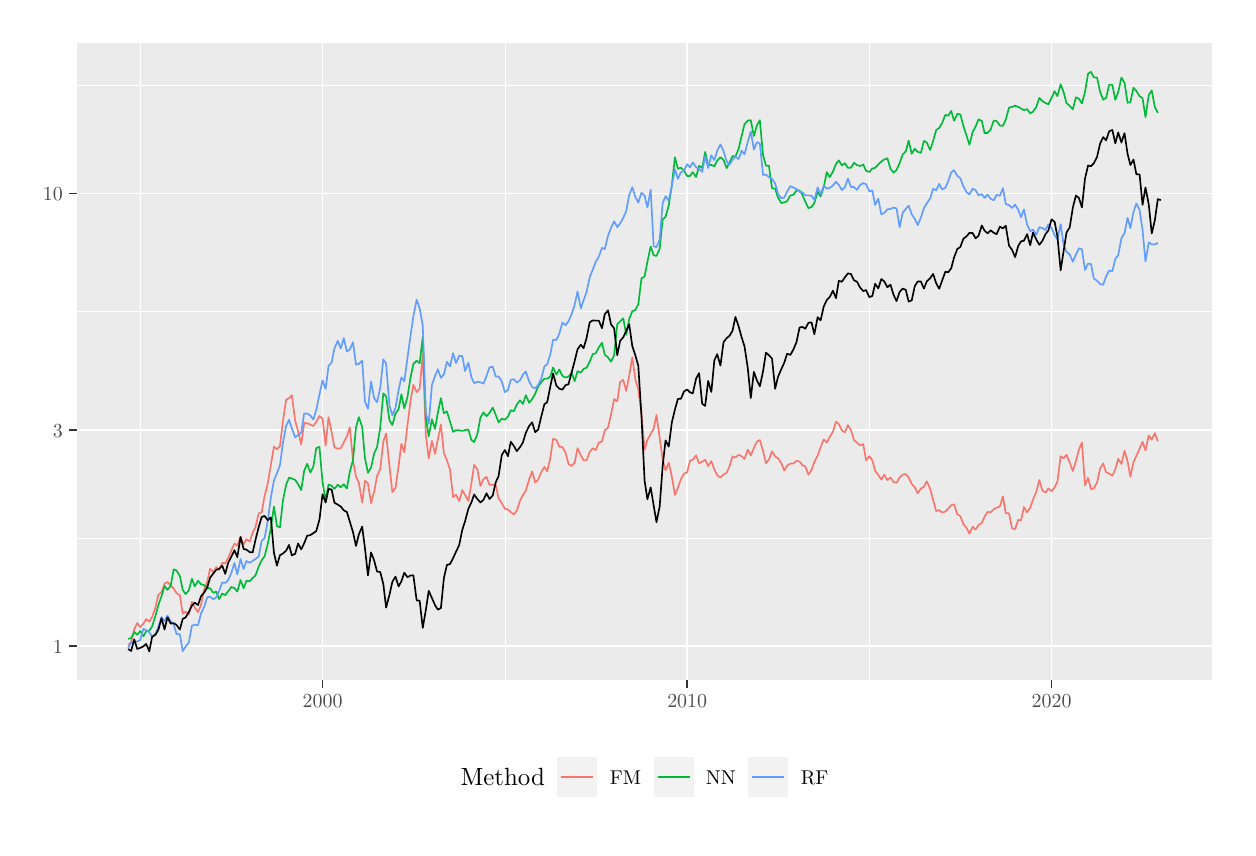
\begin{tikzpicture}[x=1pt,y=1pt]
\definecolor{fillColor}{RGB}{255,255,255}
\path[use as bounding box,fill=fillColor,fill opacity=0.00] (0,0) rectangle (433.62,289.08);
\begin{scope}
\path[clip] (  0.00,  0.00) rectangle (433.62,289.08);
\definecolor{drawColor}{RGB}{255,255,255}
\definecolor{fillColor}{RGB}{255,255,255}

\path[draw=drawColor,line width= 0.6pt,line join=round,line cap=round,fill=fillColor] (  0.00,  0.00) rectangle (433.62,289.08);
\end{scope}
\begin{scope}
\path[clip] ( 17.65, 53.26) rectangle (428.12,283.58);
\definecolor{fillColor}{gray}{0.92}

\path[fill=fillColor] ( 17.65, 53.26) rectangle (428.12,283.58);
\definecolor{drawColor}{RGB}{255,255,255}

\path[draw=drawColor,line width= 0.3pt,line join=round] ( 17.65,104.59) --
	(428.12,104.59);

\path[draw=drawColor,line width= 0.3pt,line join=round] ( 17.65,186.42) --
	(428.12,186.42);

\path[draw=drawColor,line width= 0.3pt,line join=round] ( 17.65,268.24) --
	(428.12,268.24);

\path[draw=drawColor,line width= 0.3pt,line join=round] ( 40.72, 53.26) --
	( 40.72,283.58);

\path[draw=drawColor,line width= 0.3pt,line join=round] (172.45, 53.26) --
	(172.45,283.58);

\path[draw=drawColor,line width= 0.3pt,line join=round] (304.16, 53.26) --
	(304.16,283.58);

\path[draw=drawColor,line width= 0.6pt,line join=round] ( 17.65, 65.55) --
	(428.12, 65.55);

\path[draw=drawColor,line width= 0.6pt,line join=round] ( 17.65,143.63) --
	(428.12,143.63);

\path[draw=drawColor,line width= 0.6pt,line join=round] ( 17.65,229.20) --
	(428.12,229.20);

\path[draw=drawColor,line width= 0.6pt,line join=round] (106.59, 53.26) --
	(106.59,283.58);

\path[draw=drawColor,line width= 0.6pt,line join=round] (238.32, 53.26) --
	(238.32,283.58);

\path[draw=drawColor,line width= 0.6pt,line join=round] (370.01, 53.26) --
	(370.01,283.58);
\definecolor{drawColor}{RGB}{248,118,109}

\path[draw=drawColor,line width= 0.6pt,line join=round] ( 36.31, 66.11) --
	( 37.39, 66.95) --
	( 38.51, 71.66) --
	( 39.59, 73.93) --
	( 40.67, 72.43) --
	( 41.82, 73.72) --
	( 42.83, 75.37) --
	( 43.95, 74.44) --
	( 44.96, 76.13) --
	( 46.15, 79.50) --
	( 47.23, 84.16) --
	( 48.35, 85.09) --
	( 49.47, 88.18) --
	( 50.51, 88.80) --
	( 51.67, 87.47) --
	( 52.75, 86.43) --
	( 53.80, 84.74) --
	( 54.99, 83.98) --
	( 56.03, 77.38) --
	( 57.08, 78.04) --
	( 58.23, 77.03) --
	( 59.35, 81.56) --
	( 60.36, 79.56) --
	( 61.55, 77.89) --
	( 62.63, 80.45) --
	( 63.75, 86.04) --
	( 64.87, 88.82) --
	( 65.91, 93.51) --
	( 67.07, 92.35) --
	( 68.18, 94.14) --
	( 69.19, 93.18) --
	( 70.31, 95.74) --
	( 71.39, 95.47) --
	( 72.47, 97.54) --
	( 73.59,100.18) --
	( 74.71,102.68) --
	( 75.76,101.92) --
	( 76.91,105.15) --
	( 78.03,102.25) --
	( 79.04,104.27) --
	( 80.23,103.37) --
	( 81.31,106.64) --
	( 82.32,108.62) --
	( 83.47,113.54) --
	( 84.56,113.97) --
	( 85.60,119.77) --
	( 86.75,124.37) --
	( 87.87,131.06) --
	( 88.99,137.66) --
	( 90.07,136.77) --
	( 91.15,137.80) --
	( 92.27,147.14) --
	( 93.39,154.64) --
	( 94.44,155.17) --
	( 95.45,156.28) --
	( 96.64,147.22) --
	( 97.72,143.28) --
	( 98.84,138.49) --
	( 99.92,146.23) --
	(101.00,146.12) --
	(102.15,145.66) --
	(103.23,145.12) --
	(104.28,146.61) --
	(105.43,148.75) --
	(106.55,147.80) --
	(107.67,138.12) --
	(108.72,148.32) --
	(109.83,142.95) --
	(110.84,137.43) --
	(112.03,136.94) --
	(113.12,137.10) --
	(114.23,139.20) --
	(115.35,141.41) --
	(116.40,144.67) --
	(117.55,132.72) --
	(118.63,126.90) --
	(119.68,124.63) --
	(120.87,117.42) --
	(121.88,125.32) --
	(122.96,124.43) --
	(124.08,117.25) --
	(125.20,121.37) --
	(126.24,126.96) --
	(127.40,129.59) --
	(128.51,139.56) --
	(129.52,142.43) --
	(130.71,130.75) --
	(131.79,121.27) --
	(132.91,122.81) --
	(134.03,130.63) --
	(135.04,138.71) --
	(136.09,135.64) --
	(137.24,145.48) --
	(138.36,154.33) --
	(139.37,160.05) --
	(140.56,157.42) --
	(141.64,158.63) --
	(142.76,171.28) --
	(143.88,141.82) --
	(144.92,133.39) --
	(146.07,139.78) --
	(147.19,135.07) --
	(148.20,140.13) --
	(149.32,145.64) --
	(150.40,135.42) --
	(151.48,132.80) --
	(152.60,129.41) --
	(153.72,119.44) --
	(154.77,120.32) --
	(155.92,117.99) --
	(157.04,121.97) --
	(158.05,120.23) --
	(159.24,118.02) --
	(160.32,124.32) --
	(161.33,131.09) --
	(162.52,129.47) --
	(163.60,123.47) --
	(164.72,126.03) --
	(165.80,126.78) --
	(166.88,123.87) --
	(168.04,123.96) --
	(169.12,123.81) --
	(170.16,119.00) --
	(171.32,117.25) --
	(172.44,115.21) --
	(173.55,114.95) --
	(174.56,114.03) --
	(175.68,113.20) --
	(176.73,114.49) --
	(177.88,118.08) --
	(178.96,120.19) --
	(180.01,121.86) --
	(181.20,125.79) --
	(182.28,128.74) --
	(183.40,124.73) --
	(184.48,125.77) --
	(185.56,128.48) --
	(186.72,130.38) --
	(187.72,128.74) --
	(188.84,133.45) --
	(189.85,140.48) --
	(191.04,140.16) --
	(192.12,137.65) --
	(193.24,137.51) --
	(194.36,135.50) --
	(195.41,131.45) --
	(196.56,130.69) --
	(197.64,131.88) --
	(198.69,137.16) --
	(199.88,134.48) --
	(200.89,132.75) --
	(201.97,132.73) --
	(203.09,135.81) --
	(204.20,137.13) --
	(205.25,136.45) --
	(206.40,139.13) --
	(207.52,139.55) --
	(208.53,143.49) --
	(209.72,144.61) --
	(210.80,149.31) --
	(211.92,154.85) --
	(213.04,154.05) --
	(214.09,161.07) --
	(215.20,161.78) --
	(216.29,157.78) --
	(217.37,163.36) --
	(218.48,170.00) --
	(219.60,161.90) --
	(220.65,158.33) --
	(221.80,149.44) --
	(222.92,136.53) --
	(223.93,140.14) --
	(225.12,142.23) --
	(226.20,144.14) --
	(227.21,149.13) --
	(228.37,140.93) --
	(229.45,132.99) --
	(230.49,129.06) --
	(231.65,131.89) --
	(232.76,126.90) --
	(233.88,120.20) --
	(234.96,122.82) --
	(236.05,125.89) --
	(237.16,127.92) --
	(238.28,128.35) --
	(239.33,132.61) --
	(240.34,132.99) --
	(241.53,134.55) --
	(242.61,131.65) --
	(243.73,132.27) --
	(244.81,132.91) --
	(245.89,130.69) --
	(247.04,132.46) --
	(248.13,129.39) --
	(249.17,127.36) --
	(250.33,126.49) --
	(251.44,127.63) --
	(252.56,128.23) --
	(253.57,130.44) --
	(254.69,134.18) --
	(255.74,133.79) --
	(256.89,134.70) --
	(257.97,134.27) --
	(259.02,133.22) --
	(260.21,136.58) --
	(261.29,134.51) --
	(262.41,137.21) --
	(263.49,139.50) --
	(264.57,140.04) --
	(265.72,136.13) --
	(266.77,131.70) --
	(267.85,132.99) --
	(268.97,136.02) --
	(270.09,134.11) --
	(271.13,133.48) --
	(272.29,131.77) --
	(273.41,129.01) --
	(274.41,130.81) --
	(275.60,131.55) --
	(276.69,131.62) --
	(277.80,132.52) --
	(278.92,132.32) --
	(279.93,131.02) --
	(280.98,130.50) --
	(282.13,127.52) --
	(283.25,129.26) --
	(284.26,132.17) --
	(285.45,134.44) --
	(286.53,137.48) --
	(287.65,140.33) --
	(288.77,139.19) --
	(289.81,141.12) --
	(290.97,143.07) --
	(292.08,146.72) --
	(293.09,145.84) --
	(294.21,143.55) --
	(295.29,142.84) --
	(296.38,145.46) --
	(297.49,143.65) --
	(298.61,140.01) --
	(299.66,139.15) --
	(300.81,138.13) --
	(301.93,138.60) --
	(302.94,132.79) --
	(304.13,134.23) --
	(305.21,132.73) --
	(306.22,128.93) --
	(307.37,127.45) --
	(308.46,125.79) --
	(309.50,127.52) --
	(310.66,125.59) --
	(311.77,126.50) --
	(312.89,124.91) --
	(313.97,124.60) --
	(315.06,126.51) --
	(316.17,127.59) --
	(317.29,127.77) --
	(318.34,126.59) --
	(319.45,124.22) --
	(320.57,122.94) --
	(321.62,120.79) --
	(322.77,122.52) --
	(323.85,123.19) --
	(324.90,125.16) --
	(326.09,122.45) --
	(327.17,118.48) --
	(328.29,114.42) --
	(329.37,114.75) --
	(330.45,113.87) --
	(331.61,114.23) --
	(332.62,115.25) --
	(333.73,116.55) --
	(334.74,116.81) --
	(335.93,113.24) --
	(337.02,112.56) --
	(338.13,109.65) --
	(339.25,108.37) --
	(340.30,106.22) --
	(341.45,108.73) --
	(342.53,107.71) --
	(343.58,109.33) --
	(344.77,110.10) --
	(345.78,112.39) --
	(346.86,114.10) --
	(347.98,113.94) --
	(349.10,115.10) --
	(350.14,115.61) --
	(351.30,116.03) --
	(352.41,119.72) --
	(353.42,113.61) --
	(354.61,113.58) --
	(355.70,108.20) --
	(356.81,107.87) --
	(357.93,111.25) --
	(358.94,110.99) --
	(359.99,115.87) --
	(361.14,113.89) --
	(362.26,115.64) --
	(363.27,118.57) --
	(364.46,121.35) --
	(365.54,125.63) --
	(366.66,121.86) --
	(367.78,121.09) --
	(368.82,122.54) --
	(369.98,121.59) --
	(371.09,122.93) --
	(372.10,125.07) --
	(373.26,134.22) --
	(374.34,133.50) --
	(375.38,134.73) --
	(376.54,131.91) --
	(377.66,128.85) --
	(378.77,132.44) --
	(379.86,136.55) --
	(380.94,139.22) --
	(382.06,123.70) --
	(383.17,126.41) --
	(384.22,122.34) --
	(385.23,122.56) --
	(386.42,124.74) --
	(387.50,129.72) --
	(388.62,131.62) --
	(389.70,128.41) --
	(390.78,127.97) --
	(391.94,127.17) --
	(393.02,129.51) --
	(394.06,133.28) --
	(395.22,131.41) --
	(396.34,136.17) --
	(397.45,132.34) --
	(398.46,126.86) --
	(399.58,132.08) --
	(400.63,134.37) --
	(401.78,136.92) --
	(402.86,139.46) --
	(403.91,136.34) --
	(405.10,141.76) --
	(406.18,140.20) --
	(407.30,142.58) --
	(408.38,139.56);
\definecolor{drawColor}{RGB}{0,186,56}

\path[draw=drawColor,line width= 0.6pt,line join=round] ( 36.31, 68.27) --
	( 37.39, 68.45) --
	( 38.51, 70.71) --
	( 39.59, 69.69) --
	( 40.67, 71.07) --
	( 41.82, 69.12) --
	( 42.83, 71.01) --
	( 43.95, 71.14) --
	( 44.96, 72.67) --
	( 46.15, 76.50) --
	( 47.23, 80.48) --
	( 48.35, 83.60) --
	( 49.47, 87.30) --
	( 50.51, 85.92) --
	( 51.67, 87.35) --
	( 52.75, 93.31) --
	( 53.80, 92.90) --
	( 54.99, 90.96) --
	( 56.03, 85.90) --
	( 57.08, 84.41) --
	( 58.23, 85.70) --
	( 59.35, 89.93) --
	( 60.36, 87.18) --
	( 61.55, 89.19) --
	( 62.63, 87.99) --
	( 63.75, 87.62) --
	( 64.87, 86.68) --
	( 65.91, 86.48) --
	( 67.07, 84.89) --
	( 68.18, 85.30) --
	( 69.19, 82.59) --
	( 70.31, 84.59) --
	( 71.39, 84.01) --
	( 72.47, 85.45) --
	( 73.59, 86.99) --
	( 74.71, 86.53) --
	( 75.76, 85.31) --
	( 76.91, 89.52) --
	( 78.03, 86.50) --
	( 79.04, 89.28) --
	( 80.23, 89.00) --
	( 81.31, 90.26) --
	( 82.32, 91.15) --
	( 83.47, 94.30) --
	( 84.56, 96.64) --
	( 85.60, 98.06) --
	( 86.75,102.46) --
	( 87.87,108.32) --
	( 88.99,116.00) --
	( 90.07,109.03) --
	( 91.15,108.47) --
	( 92.27,118.39) --
	( 93.39,123.93) --
	( 94.44,126.49) --
	( 95.45,126.21) --
	( 96.64,125.64) --
	( 97.72,124.10) --
	( 98.84,121.98) --
	( 99.92,128.99) --
	(101.00,131.47) --
	(102.15,128.34) --
	(103.23,130.45) --
	(104.28,137.16) --
	(105.43,137.60) --
	(106.55,124.86) --
	(107.67,118.32) --
	(108.72,123.99) --
	(109.83,123.60) --
	(110.84,122.42) --
	(112.03,123.90) --
	(113.12,123.00) --
	(114.23,124.12) --
	(115.35,122.54) --
	(116.40,128.60) --
	(117.55,132.73) --
	(118.63,144.58) --
	(119.68,148.35) --
	(120.87,144.81) --
	(121.88,133.46) --
	(122.96,128.24) --
	(124.08,130.12) --
	(125.20,135.21) --
	(126.24,137.46) --
	(127.40,144.60) --
	(128.51,156.96) --
	(129.52,155.86) --
	(130.71,147.29) --
	(131.79,145.47) --
	(132.91,149.67) --
	(134.03,151.16) --
	(135.04,156.59) --
	(136.09,151.52) --
	(137.24,155.61) --
	(138.36,162.80) --
	(139.37,167.56) --
	(140.56,168.74) --
	(141.64,167.82) --
	(142.76,177.31) --
	(143.88,148.06) --
	(144.92,141.39) --
	(146.07,147.61) --
	(147.19,144.06) --
	(148.20,149.89) --
	(149.32,155.21) --
	(150.40,149.71) --
	(151.48,150.45) --
	(152.60,146.79) --
	(153.72,143.02) --
	(154.77,143.64) --
	(155.92,143.59) --
	(157.04,143.36) --
	(158.05,143.68) --
	(159.24,143.86) --
	(160.32,140.14) --
	(161.33,139.32) --
	(162.52,142.32) --
	(163.60,148.20) --
	(164.72,150.08) --
	(165.80,148.69) --
	(166.88,149.90) --
	(168.04,151.80) --
	(169.12,149.21) --
	(170.16,146.48) --
	(171.32,147.82) --
	(172.44,147.42) --
	(173.55,148.54) --
	(174.56,150.84) --
	(175.68,150.49) --
	(176.73,152.86) --
	(177.88,154.42) --
	(178.96,153.11) --
	(180.01,156.26) --
	(181.20,153.55) --
	(182.28,154.87) --
	(183.40,156.84) --
	(184.48,159.45) --
	(185.56,160.91) --
	(186.72,162.25) --
	(187.72,162.26) --
	(188.84,162.98) --
	(189.85,166.29) --
	(191.04,163.71) --
	(192.12,165.54) --
	(193.24,163.24) --
	(194.36,162.66) --
	(195.41,162.94) --
	(196.56,164.34) --
	(197.64,161.33) --
	(198.69,164.96) --
	(199.88,164.41) --
	(200.89,165.77) --
	(201.97,166.22) --
	(203.09,168.44) --
	(204.20,171.13) --
	(205.25,171.40) --
	(206.40,173.58) --
	(207.52,175.23) --
	(208.53,170.93) --
	(209.72,169.92) --
	(210.80,168.37) --
	(211.92,170.70) --
	(213.04,181.95) --
	(214.09,182.96) --
	(215.20,184.07) --
	(216.29,178.13) --
	(217.37,183.83) --
	(218.48,186.62) --
	(219.60,187.08) --
	(220.65,189.12) --
	(221.80,198.49) --
	(222.92,199.19) --
	(223.93,204.41) --
	(225.12,210.02) --
	(226.20,206.81) --
	(227.21,206.60) --
	(228.37,209.17) --
	(229.45,219.82) --
	(230.49,220.69) --
	(231.65,224.84) --
	(232.76,232.06) --
	(233.88,242.25) --
	(234.96,238.10) --
	(236.05,238.51) --
	(237.16,237.37) --
	(238.28,235.48) --
	(239.33,235.48) --
	(240.34,236.89) --
	(241.53,235.08) --
	(242.61,239.17) --
	(243.73,238.34) --
	(244.81,244.16) --
	(245.89,239.38) --
	(247.04,239.49) --
	(248.13,238.98) --
	(249.17,241.02) --
	(250.33,242.29) --
	(251.44,241.29) --
	(252.56,238.31) --
	(253.57,240.31) --
	(254.69,242.68) --
	(255.74,242.52) --
	(256.89,245.32) --
	(257.97,249.86) --
	(259.02,254.21) --
	(260.21,255.51) --
	(261.29,255.64) --
	(262.41,249.93) --
	(263.49,253.78) --
	(264.57,255.64) --
	(265.72,243.05) --
	(266.77,239.23) --
	(267.85,239.16) --
	(268.97,231.04) --
	(270.09,230.87) --
	(271.13,227.72) --
	(272.29,225.71) --
	(273.41,225.95) --
	(274.41,226.34) --
	(275.60,228.45) --
	(276.69,228.69) --
	(277.80,230.25) --
	(278.92,230.29) --
	(279.93,228.69) --
	(280.98,226.23) --
	(282.13,223.84) --
	(283.25,224.33) --
	(284.26,225.73) --
	(285.45,229.74) --
	(286.53,228.12) --
	(287.65,231.49) --
	(288.77,236.88) --
	(289.81,235.06) --
	(290.97,237.03) --
	(292.08,239.84) --
	(293.09,241.13) --
	(294.21,239.31) --
	(295.29,240.09) --
	(296.38,238.45) --
	(297.49,238.48) --
	(298.61,240.26) --
	(299.66,239.41) --
	(300.81,239.09) --
	(301.93,239.64) --
	(302.94,237.38) --
	(304.13,236.93) --
	(305.21,238.18) --
	(306.22,238.42) --
	(307.37,239.64) --
	(308.46,240.71) --
	(309.50,241.43) --
	(310.66,241.88) --
	(311.77,238.11) --
	(312.89,236.67) --
	(313.97,237.66) --
	(315.06,240.11) --
	(316.17,243.20) --
	(317.29,244.38) --
	(318.34,248.24) --
	(319.45,243.50) --
	(320.57,245.31) --
	(321.62,244.19) --
	(322.77,243.87) --
	(323.85,248.15) --
	(324.90,247.58) --
	(326.09,244.85) --
	(327.17,248.07) --
	(328.29,252.09) --
	(329.37,252.85) --
	(330.45,254.63) --
	(331.61,257.60) --
	(332.62,257.22) --
	(333.73,258.99) --
	(334.74,255.44) --
	(335.93,257.93) --
	(337.02,257.74) --
	(338.13,253.53) --
	(339.25,250.08) --
	(340.30,246.78) --
	(341.45,251.38) --
	(342.53,253.32) --
	(343.58,255.92) --
	(344.77,255.42) --
	(345.78,250.98) --
	(346.86,251.03) --
	(347.98,252.33) --
	(349.10,255.52) --
	(350.14,255.31) --
	(351.30,253.71) --
	(352.41,253.62) --
	(353.42,255.83) --
	(354.61,260.16) --
	(355.70,260.44) --
	(356.81,260.88) --
	(357.93,260.40) --
	(358.94,259.89) --
	(359.99,259.27) --
	(361.14,259.65) --
	(362.26,258.10) --
	(363.27,258.74) --
	(364.46,260.42) --
	(365.54,263.68) --
	(366.66,262.57) --
	(367.78,261.84) --
	(368.82,261.39) --
	(369.98,263.68) --
	(371.09,266.14) --
	(372.10,264.34) --
	(373.26,268.64) --
	(374.34,265.76) --
	(375.38,261.80) --
	(376.54,260.80) --
	(377.66,259.56) --
	(378.77,263.89) --
	(379.86,263.43) --
	(380.94,261.72) --
	(382.06,265.83) --
	(383.17,272.47) --
	(384.22,273.11) --
	(385.23,271.15) --
	(386.42,271.02) --
	(387.50,265.95) --
	(388.62,263.02) --
	(389.70,263.74) --
	(390.78,268.41) --
	(391.94,268.43) --
	(393.02,262.97) --
	(394.06,265.79) --
	(395.22,271.03) --
	(396.34,269.17) --
	(397.45,261.93) --
	(398.46,262.19) --
	(399.58,267.37) --
	(400.63,266.19) --
	(401.78,264.31) --
	(402.86,263.59) --
	(403.91,256.77) --
	(405.10,264.70) --
	(406.18,266.37) --
	(407.30,260.42) --
	(408.38,258.30);
\definecolor{drawColor}{RGB}{97,156,255}

\path[draw=drawColor,line width= 0.6pt,line join=round] ( 36.31, 64.92) --
	( 37.39, 66.96) --
	( 38.51, 67.14) --
	( 39.59, 67.28) --
	( 40.67, 67.82) --
	( 41.82, 71.86) --
	( 42.83, 71.35) --
	( 43.95, 70.61) --
	( 44.96, 69.08) --
	( 46.15, 70.09) --
	( 47.23, 72.60) --
	( 48.35, 76.12) --
	( 49.47, 74.58) --
	( 50.51, 76.65) --
	( 51.67, 74.59) --
	( 52.75, 73.55) --
	( 53.80, 69.99) --
	( 54.99, 69.87) --
	( 56.03, 63.79) --
	( 57.08, 65.46) --
	( 58.23, 66.88) --
	( 59.35, 72.94) --
	( 60.36, 73.38) --
	( 61.55, 73.15) --
	( 62.63, 77.40) --
	( 63.75, 79.69) --
	( 64.87, 83.25) --
	( 65.91, 83.46) --
	( 67.07, 82.54) --
	( 68.18, 83.22) --
	( 69.19, 85.53) --
	( 70.31, 88.59) --
	( 71.39, 88.44) --
	( 72.47, 89.49) --
	( 73.59, 92.03) --
	( 74.71, 95.71) --
	( 75.76, 91.47) --
	( 76.91, 97.07) --
	( 78.03, 93.48) --
	( 79.04, 96.36) --
	( 80.23, 95.74) --
	( 81.31, 96.42) --
	( 82.32, 97.09) --
	( 83.47, 98.00) --
	( 84.56,103.68) --
	( 85.60,104.59) --
	( 86.75,110.82) --
	( 87.87,119.25) --
	( 88.99,125.48) --
	( 90.07,128.03) --
	( 91.15,130.93) --
	( 92.27,139.28) --
	( 93.39,145.17) --
	( 94.44,147.40) --
	( 95.45,144.31) --
	( 96.64,141.07) --
	( 97.72,141.84) --
	( 98.84,142.74) --
	( 99.92,149.71) --
	(101.00,149.64) --
	(102.15,148.95) --
	(103.23,147.45) --
	(104.28,150.94) --
	(105.43,156.50) --
	(106.55,161.57) --
	(107.67,158.54) --
	(108.72,166.85) --
	(109.83,168.08) --
	(110.84,173.14) --
	(112.03,175.90) --
	(113.12,173.17) --
	(114.23,176.90) --
	(115.35,172.05) --
	(116.40,172.79) --
	(117.55,175.45) --
	(118.63,167.32) --
	(119.68,167.57) --
	(120.87,168.74) --
	(121.88,153.98) --
	(122.96,151.35) --
	(124.08,161.25) --
	(125.20,155.13) --
	(126.24,153.75) --
	(127.40,158.95) --
	(128.51,169.21) --
	(129.52,167.72) --
	(130.71,152.67) --
	(131.79,148.96) --
	(132.91,151.69) --
	(134.03,158.16) --
	(135.04,162.73) --
	(136.09,161.31) --
	(137.24,169.73) --
	(138.36,177.90) --
	(139.37,184.78) --
	(140.56,190.78) --
	(141.64,187.65) --
	(142.76,181.49) --
	(143.88,149.79) --
	(144.92,145.98) --
	(146.07,159.97) --
	(147.19,163.16) --
	(148.20,165.67) --
	(149.32,162.52) --
	(150.40,163.80) --
	(151.48,168.33) --
	(152.60,166.66) --
	(153.72,171.47) --
	(154.77,167.87) --
	(155.92,170.52) --
	(157.04,170.40) --
	(158.05,165.00) --
	(159.24,168.03) --
	(160.32,162.86) --
	(161.33,160.61) --
	(162.52,161.12) --
	(163.60,160.92) --
	(164.72,160.46) --
	(165.80,163.26) --
	(166.88,166.33) --
	(168.04,166.60) --
	(169.12,163.00) --
	(170.16,163.00) --
	(171.32,161.24) --
	(172.44,157.38) --
	(173.55,158.14) --
	(174.56,161.82) --
	(175.68,162.07) --
	(176.73,160.83) --
	(177.88,161.63) --
	(178.96,163.69) --
	(180.01,164.84) --
	(181.20,161.30) --
	(182.28,159.26) --
	(183.40,158.75) --
	(184.48,160.03) --
	(185.56,162.19) --
	(186.72,166.66) --
	(187.72,167.49) --
	(188.84,170.92) --
	(189.85,176.30) --
	(191.04,176.24) --
	(192.12,178.56) --
	(193.24,182.54) --
	(194.36,181.58) --
	(195.41,182.96) --
	(196.56,185.57) --
	(197.64,188.87) --
	(198.69,193.76) --
	(199.88,187.63) --
	(200.89,190.60) --
	(201.97,193.63) --
	(203.09,198.87) --
	(204.20,201.69) --
	(205.25,204.41) --
	(206.40,206.42) --
	(207.52,209.49) --
	(208.53,209.07) --
	(209.72,213.91) --
	(210.80,216.75) --
	(211.92,219.13) --
	(213.04,217.02) --
	(214.09,218.33) --
	(215.20,220.36) --
	(216.29,222.83) --
	(217.37,228.63) --
	(218.48,231.46) --
	(219.60,227.89) --
	(220.65,225.90) --
	(221.80,229.43) --
	(222.92,228.40) --
	(223.93,224.09) --
	(225.12,230.50) --
	(226.20,210.13) --
	(227.21,209.74) --
	(228.37,212.45) --
	(229.45,225.72) --
	(230.49,228.17) --
	(231.65,226.54) --
	(232.76,231.91) --
	(233.88,237.86) --
	(234.96,234.46) --
	(236.05,236.85) --
	(237.16,237.28) --
	(238.28,239.77) --
	(239.33,238.62) --
	(240.34,240.37) --
	(241.53,238.65) --
	(242.61,238.02) --
	(243.73,236.97) --
	(244.81,242.61) --
	(245.89,238.39) --
	(247.04,242.96) --
	(248.13,241.21) --
	(249.17,244.65) --
	(250.33,246.91) --
	(251.44,244.48) --
	(252.56,240.76) --
	(253.57,239.54) --
	(254.69,241.26) --
	(255.74,242.50) --
	(256.89,241.59) --
	(257.97,244.62) --
	(259.02,243.34) --
	(260.21,247.80) --
	(261.29,251.59) --
	(262.41,245.04) --
	(263.49,247.68) --
	(264.57,247.25) --
	(265.72,235.87) --
	(266.77,235.98) --
	(267.85,235.08) --
	(268.97,234.45) --
	(270.09,232.80) --
	(271.13,228.95) --
	(272.29,227.46) --
	(273.41,227.69) --
	(274.41,229.85) --
	(275.60,231.83) --
	(276.69,231.29) --
	(277.80,230.78) --
	(278.92,229.76) --
	(279.93,229.56) --
	(280.98,228.55) --
	(282.13,228.45) --
	(283.25,228.34) --
	(284.26,226.87) --
	(285.45,231.34) --
	(286.53,228.85) --
	(287.65,231.96) --
	(288.77,230.93) --
	(289.81,231.18) --
	(290.97,232.04) --
	(292.08,233.43) --
	(293.09,232.28) --
	(294.21,230.41) --
	(295.29,231.36) --
	(296.38,234.54) --
	(297.49,231.49) --
	(298.61,231.50) --
	(299.66,230.45) --
	(300.81,232.26) --
	(301.93,232.91) --
	(302.94,232.52) --
	(304.13,229.96) --
	(305.21,230.22) --
	(306.22,225.00) --
	(307.37,227.25) --
	(308.46,221.60) --
	(309.50,222.16) --
	(310.66,223.43) --
	(311.77,223.58) --
	(312.89,224.08) --
	(313.97,223.76) --
	(315.06,216.96) --
	(316.17,222.17) --
	(317.29,223.60) --
	(318.34,224.78) --
	(319.45,221.62) --
	(320.57,219.96) --
	(321.62,217.73) --
	(322.77,220.47) --
	(323.85,223.86) --
	(324.90,225.62) --
	(326.09,227.33) --
	(327.17,230.85) --
	(328.29,230.31) --
	(329.37,232.63) --
	(330.45,230.62) --
	(331.61,231.23) --
	(332.62,233.57) --
	(333.73,236.82) --
	(334.74,237.58) --
	(335.93,235.51) --
	(337.02,234.66) --
	(338.13,231.70) --
	(339.25,229.65) --
	(340.30,228.82) --
	(341.45,230.90) --
	(342.53,230.35) --
	(343.58,228.51) --
	(344.77,228.95) --
	(345.78,227.57) --
	(346.86,228.78) --
	(347.98,227.21) --
	(349.10,226.70) --
	(350.14,228.68) --
	(351.30,228.32) --
	(352.41,231.06) --
	(353.42,225.40) --
	(354.61,224.95) --
	(355.70,223.93) --
	(356.81,225.10) --
	(357.93,223.27) --
	(358.94,220.51) --
	(359.99,223.42) --
	(361.14,217.94) --
	(362.26,215.49) --
	(363.27,216.11) --
	(364.46,214.27) --
	(365.54,216.96) --
	(366.66,216.69) --
	(367.78,215.95) --
	(368.82,217.99) --
	(369.98,216.68) --
	(371.09,214.10) --
	(372.10,212.59) --
	(373.26,218.09) --
	(374.34,210.68) --
	(375.38,208.02) --
	(376.54,207.16) --
	(377.66,204.52) --
	(378.77,207.09) --
	(379.86,209.36) --
	(380.94,208.99) --
	(382.06,201.53) --
	(383.17,203.80) --
	(384.22,203.66) --
	(385.23,198.48) --
	(386.42,197.62) --
	(387.50,196.48) --
	(388.62,196.14) --
	(389.70,199.21) --
	(390.78,201.32) --
	(391.94,201.10) --
	(393.02,205.53) --
	(394.06,206.84) --
	(395.22,213.01) --
	(396.34,214.85) --
	(397.45,220.36) --
	(398.46,216.67) --
	(399.58,222.50) --
	(400.63,225.55) --
	(401.78,223.22) --
	(402.86,215.92) --
	(403.91,204.59) --
	(405.10,211.51) --
	(406.18,210.81) --
	(407.30,210.72) --
	(408.38,211.34);
\definecolor{drawColor}{RGB}{0,0,0}

\path[draw=drawColor,line width= 0.6pt,line join=round] ( 36.31, 64.56) --
	( 37.39, 63.84) --
	( 38.51, 68.05) --
	( 39.59, 64.58) --
	( 40.67, 64.96) --
	( 41.82, 65.55) --
	( 42.83, 66.40) --
	( 43.95, 63.73) --
	( 44.96, 68.94) --
	( 46.15, 69.68) --
	( 47.23, 71.51) --
	( 48.35, 75.66) --
	( 49.47, 71.58) --
	( 50.51, 76.03) --
	( 51.67, 73.72) --
	( 52.75, 73.90) --
	( 53.80, 73.24) --
	( 54.99, 71.58) --
	( 56.03, 75.45) --
	( 57.08, 75.97) --
	( 58.23, 77.91) --
	( 59.35, 80.22) --
	( 60.36, 81.33) --
	( 61.55, 80.45) --
	( 62.63, 83.60) --
	( 63.75, 84.93) --
	( 64.87, 86.76) --
	( 65.91, 90.30) --
	( 67.07, 91.86) --
	( 68.18, 93.20) --
	( 69.19, 93.53) --
	( 70.31, 94.67) --
	( 71.39, 91.71) --
	( 72.47, 95.76) --
	( 73.59, 97.96) --
	( 74.71,100.24) --
	( 75.76, 97.71) --
	( 76.91,105.03) --
	( 78.03,100.70) --
	( 79.04,100.48) --
	( 80.23, 99.57) --
	( 81.31, 99.47) --
	( 82.32,104.00) --
	( 83.47,108.57) --
	( 84.56,112.28) --
	( 85.60,112.65) --
	( 86.75,111.12) --
	( 87.87,112.12) --
	( 88.99, 99.32) --
	( 90.07, 94.67) --
	( 91.15, 98.45) --
	( 92.27, 99.08) --
	( 93.39,100.11) --
	( 94.44,102.15) --
	( 95.45, 98.40) --
	( 96.64, 98.93) --
	( 97.72,102.70) --
	( 98.84,100.59) --
	( 99.92,102.78) --
	(101.00,105.49) --
	(102.15,105.73) --
	(103.23,106.43) --
	(104.28,107.17) --
	(105.43,111.32) --
	(106.55,120.49) --
	(107.67,117.48) --
	(108.72,122.38) --
	(109.83,122.20) --
	(110.84,117.44) --
	(112.03,116.75) --
	(113.12,116.05) --
	(114.23,114.67) --
	(115.35,114.07) --
	(116.40,110.61) --
	(117.55,106.83) --
	(118.63,101.80) --
	(119.68,106.00) --
	(120.87,108.80) --
	(121.88,100.93) --
	(122.96, 91.16) --
	(124.08, 99.48) --
	(125.20, 96.55) --
	(126.24, 92.54) --
	(127.40, 92.37) --
	(128.51, 88.04) --
	(129.52, 79.53) --
	(130.71, 84.08) --
	(131.79, 88.88) --
	(132.91, 90.71) --
	(134.03, 87.15) --
	(135.04, 89.05) --
	(136.09, 92.14) --
	(137.24, 90.50) --
	(138.36, 91.14) --
	(139.37, 91.19) --
	(140.56, 82.12) --
	(141.64, 82.01) --
	(142.76, 72.18) --
	(143.88, 78.71) --
	(144.92, 85.61) --
	(146.07, 82.97) --
	(147.19, 80.45) --
	(148.20, 78.79) --
	(149.32, 79.34) --
	(150.40, 90.16) --
	(151.48, 94.93) --
	(152.60, 95.24) --
	(153.72, 97.38) --
	(154.77, 99.68) --
	(155.92,102.08) --
	(157.04,107.60) --
	(158.05,110.73) --
	(159.24,115.23) --
	(160.32,117.48) --
	(161.33,120.39) --
	(162.52,118.73) --
	(163.60,117.49) --
	(164.72,118.50) --
	(165.80,120.83) --
	(166.88,118.75) --
	(168.04,120.02) --
	(169.12,124.75) --
	(170.16,127.03) --
	(171.32,134.68) --
	(172.44,136.47) --
	(173.55,134.24) --
	(174.56,139.44) --
	(175.68,137.95) --
	(176.73,136.05) --
	(177.88,137.46) --
	(178.96,139.22) --
	(180.01,142.71) --
	(181.20,145.13) --
	(182.28,146.46) --
	(183.40,142.90) --
	(184.48,143.87) --
	(185.56,148.45) --
	(186.72,153.02) --
	(187.72,153.74) --
	(188.84,159.37) --
	(189.85,164.10) --
	(191.04,159.77) --
	(192.12,158.61) --
	(193.24,158.28) --
	(194.36,159.92) --
	(195.41,160.22) --
	(196.56,164.47) --
	(197.64,168.57) --
	(198.69,172.84) --
	(199.88,174.52) --
	(200.89,173.28) --
	(201.97,176.98) --
	(203.09,182.63) --
	(204.20,183.29) --
	(205.25,183.21) --
	(206.40,183.20) --
	(207.52,180.47) --
	(208.53,185.55) --
	(209.72,186.94) --
	(210.80,181.83) --
	(211.92,180.46) --
	(213.04,170.73) --
	(214.09,175.89) --
	(215.20,177.19) --
	(216.29,179.49) --
	(217.37,181.92) --
	(218.48,173.97) --
	(219.60,170.61) --
	(220.65,166.87) --
	(221.80,148.64) --
	(222.92,125.37) --
	(223.93,118.66) --
	(225.12,122.96) --
	(226.20,116.47) --
	(227.21,110.39) --
	(228.37,116.08) --
	(229.45,130.64) --
	(230.49,139.93) --
	(231.65,137.69) --
	(232.76,146.40) --
	(233.88,151.11) --
	(234.96,154.94) --
	(236.05,154.99) --
	(237.16,157.62) --
	(238.28,158.33) --
	(239.33,157.30) --
	(240.34,156.92) --
	(241.53,162.29) --
	(242.61,164.24) --
	(243.73,153.20) --
	(244.81,152.41) --
	(245.89,161.43) --
	(247.04,157.45) --
	(248.13,168.90) --
	(249.17,171.11) --
	(250.33,166.98) --
	(251.44,175.41) --
	(252.56,176.89) --
	(253.57,177.68) --
	(254.69,179.54) --
	(255.74,184.56) --
	(256.89,181.19) --
	(257.97,177.22) --
	(259.02,173.95) --
	(260.21,166.06) --
	(261.29,155.22) --
	(262.41,164.70) --
	(263.49,161.68) --
	(264.57,159.47) --
	(265.72,164.87) --
	(266.77,171.65) --
	(267.85,170.73) --
	(268.97,169.49) --
	(270.09,158.59) --
	(271.13,162.89) --
	(272.29,165.61) --
	(273.41,168.08) --
	(274.41,171.23) --
	(275.60,170.83) --
	(276.69,172.79) --
	(277.80,175.42) --
	(278.92,180.72) --
	(279.93,180.97) --
	(280.98,180.29) --
	(282.13,182.43) --
	(283.25,182.59) --
	(284.26,178.29) --
	(285.45,184.47) --
	(286.53,183.35) --
	(287.65,188.32) --
	(288.77,190.69) --
	(289.81,191.77) --
	(290.97,194.03) --
	(292.08,191.36) --
	(293.09,197.60) --
	(294.21,197.26) --
	(295.29,198.85) --
	(296.38,200.28) --
	(297.49,200.08) --
	(298.61,197.75) --
	(299.66,197.32) --
	(300.81,195.14) --
	(301.93,193.90) --
	(302.94,194.26) --
	(304.13,191.70) --
	(305.21,192.13) --
	(306.22,196.52) --
	(307.37,194.88) --
	(308.46,198.25) --
	(309.50,197.41) --
	(310.66,195.28) --
	(311.77,196.24) --
	(312.89,192.51) --
	(313.97,190.26) --
	(315.06,193.54) --
	(316.17,194.79) --
	(317.29,194.36) --
	(318.34,190.07) --
	(319.45,190.57) --
	(320.57,195.75) --
	(321.62,197.37) --
	(322.77,197.36) --
	(323.85,194.78) --
	(324.90,197.43) --
	(326.09,198.52) --
	(327.17,200.11) --
	(328.29,196.72) --
	(329.37,194.73) --
	(330.45,197.74) --
	(331.61,200.95) --
	(332.62,200.65) --
	(333.73,202.15) --
	(334.74,206.05) --
	(335.93,209.11) --
	(337.02,209.85) --
	(338.13,212.83) --
	(339.25,213.68) --
	(340.30,214.94) --
	(341.45,214.86) --
	(342.53,212.97) --
	(343.58,213.83) --
	(344.77,217.61) --
	(345.78,215.70) --
	(346.86,214.77) --
	(347.98,215.84) --
	(349.10,214.95) --
	(350.14,214.45) --
	(351.30,217.18) --
	(352.41,216.55) --
	(353.42,217.52) --
	(354.61,210.31) --
	(355.70,208.81) --
	(356.81,206.15) --
	(357.93,210.22) --
	(358.94,211.85) --
	(359.99,212.11) --
	(361.14,214.49) --
	(362.26,210.47) --
	(363.27,215.03) --
	(364.46,212.56) --
	(365.54,210.62) --
	(366.66,212.04) --
	(367.78,214.47) --
	(368.82,215.81) --
	(369.98,219.82) --
	(371.09,218.88) --
	(372.10,213.62) --
	(373.26,201.40) --
	(374.34,208.41) --
	(375.38,215.05) --
	(376.54,216.91) --
	(377.66,224.03) --
	(378.77,228.39) --
	(379.86,227.57) --
	(380.94,224.13) --
	(382.06,234.53) --
	(383.17,239.27) --
	(384.22,239.02) --
	(385.23,240.06) --
	(386.42,242.42) --
	(387.50,247.13) --
	(388.62,249.52) --
	(389.70,248.33) --
	(390.78,251.62) --
	(391.94,252.11) --
	(393.02,247.28) --
	(394.06,251.21) --
	(395.22,247.55) --
	(396.34,250.95) --
	(397.45,243.45) --
	(398.46,239.44) --
	(399.58,241.41) --
	(400.63,236.10) --
	(401.78,236.06) --
	(402.86,225.07) --
	(403.91,231.37) --
	(405.10,225.21) --
	(406.18,214.72) --
	(407.30,219.51) --
	(408.38,227.11) --
	(409.46,226.78);
\end{scope}
\begin{scope}
\path[clip] (  0.00,  0.00) rectangle (433.62,289.08);
\definecolor{drawColor}{gray}{0.30}

\node[text=drawColor,anchor=base east,inner sep=0pt, outer sep=0pt, scale=  0.72] at ( 12.70, 63.07) {1};

\node[text=drawColor,anchor=base east,inner sep=0pt, outer sep=0pt, scale=  0.72] at ( 12.70,141.15) {3};

\node[text=drawColor,anchor=base east,inner sep=0pt, outer sep=0pt, scale=  0.72] at ( 12.70,226.72) {10};
\end{scope}
\begin{scope}
\path[clip] (  0.00,  0.00) rectangle (433.62,289.08);
\definecolor{drawColor}{gray}{0.20}

\path[draw=drawColor,line width= 0.6pt,line join=round] ( 14.90, 65.55) --
	( 17.65, 65.55);

\path[draw=drawColor,line width= 0.6pt,line join=round] ( 14.90,143.63) --
	( 17.65,143.63);

\path[draw=drawColor,line width= 0.6pt,line join=round] ( 14.90,229.20) --
	( 17.65,229.20);
\end{scope}
\begin{scope}
\path[clip] (  0.00,  0.00) rectangle (433.62,289.08);
\definecolor{drawColor}{gray}{0.20}

\path[draw=drawColor,line width= 0.6pt,line join=round] (106.59, 50.51) --
	(106.59, 53.26);

\path[draw=drawColor,line width= 0.6pt,line join=round] (238.32, 50.51) --
	(238.32, 53.26);

\path[draw=drawColor,line width= 0.6pt,line join=round] (370.01, 50.51) --
	(370.01, 53.26);
\end{scope}
\begin{scope}
\path[clip] (  0.00,  0.00) rectangle (433.62,289.08);
\definecolor{drawColor}{gray}{0.30}

\node[text=drawColor,anchor=base,inner sep=0pt, outer sep=0pt, scale=  0.72] at (106.59, 43.35) {2000};

\node[text=drawColor,anchor=base,inner sep=0pt, outer sep=0pt, scale=  0.72] at (238.32, 43.35) {2010};

\node[text=drawColor,anchor=base,inner sep=0pt, outer sep=0pt, scale=  0.72] at (370.01, 43.35) {2020};
\end{scope}
\begin{scope}
\path[clip] (  0.00,  0.00) rectangle (433.62,289.08);
\definecolor{fillColor}{RGB}{255,255,255}

\path[fill=fillColor] (150.91,  5.50) rectangle (294.86, 30.95);
\end{scope}
\begin{scope}
\path[clip] (  0.00,  0.00) rectangle (433.62,289.08);
\definecolor{drawColor}{RGB}{0,0,0}

\node[text=drawColor,anchor=base west,inner sep=0pt, outer sep=0pt, scale=  0.90] at (156.41, 15.13) {Method};
\end{scope}
\begin{scope}
\path[clip] (  0.00,  0.00) rectangle (433.62,289.08);
\definecolor{fillColor}{gray}{0.95}

\path[fill=fillColor] (191.40, 11.00) rectangle (205.86, 25.45);
\end{scope}
\begin{scope}
\path[clip] (  0.00,  0.00) rectangle (433.62,289.08);
\definecolor{drawColor}{RGB}{248,118,109}

\path[draw=drawColor,line width= 0.6pt,line join=round] (192.85, 18.23) -- (204.41, 18.23);
\end{scope}
\begin{scope}
\path[clip] (  0.00,  0.00) rectangle (433.62,289.08);
\definecolor{fillColor}{gray}{0.95}

\path[fill=fillColor] (226.15, 11.00) rectangle (240.61, 25.45);
\end{scope}
\begin{scope}
\path[clip] (  0.00,  0.00) rectangle (433.62,289.08);
\definecolor{drawColor}{RGB}{0,186,56}

\path[draw=drawColor,line width= 0.6pt,line join=round] (227.60, 18.23) -- (239.16, 18.23);
\end{scope}
\begin{scope}
\path[clip] (  0.00,  0.00) rectangle (433.62,289.08);
\definecolor{fillColor}{gray}{0.95}

\path[fill=fillColor] (260.41, 11.00) rectangle (274.86, 25.45);
\end{scope}
\begin{scope}
\path[clip] (  0.00,  0.00) rectangle (433.62,289.08);
\definecolor{drawColor}{RGB}{97,156,255}

\path[draw=drawColor,line width= 0.6pt,line join=round] (261.85, 18.23) -- (273.41, 18.23);
\end{scope}
\begin{scope}
\path[clip] (  0.00,  0.00) rectangle (433.62,289.08);
\definecolor{drawColor}{RGB}{0,0,0}

\node[text=drawColor,anchor=base west,inner sep=0pt, outer sep=0pt, scale=  0.72] at (210.36, 15.75) {FM};
\end{scope}
\begin{scope}
\path[clip] (  0.00,  0.00) rectangle (433.62,289.08);
\definecolor{drawColor}{RGB}{0,0,0}

\node[text=drawColor,anchor=base west,inner sep=0pt, outer sep=0pt, scale=  0.72] at (245.11, 15.75) {NN};
\end{scope}
\begin{scope}
\path[clip] (  0.00,  0.00) rectangle (433.62,289.08);
\definecolor{drawColor}{RGB}{0,0,0}

\node[text=drawColor,anchor=base west,inner sep=0pt, outer sep=0pt, scale=  0.72] at (279.36, 15.75) {RF};
\end{scope}
\end{tikzpicture}

\label{plot:cumul_vw_LS_portf_return}
\end{figure}

Figures \ref{plot:cumul_ew_LS_portf_return} and \ref{plot:cumul_vw_LS_portf_return} show the cumulative return of the equal and value-weighted long-short portfolios from July 1994 to November 2022. As a benchmark value weighted market value is plotted to these figures as well. As can be seen from Figure \ref{plot:cumul_ew_portf_return} among equal-weighted portfolios random forest approach provides the largest spread between the lowest and highest expected return portfolios. For linear regression and neural network models the spread is almost identical. Figure \ref{plot:cumul_ew_portf_return} shows that the high expected return portfolio of the linear model performs better than the high expected return portfolio of the neural network, but the neural network model does a better job picking low expected return companies. \par

An interesting remark from Figure \ref{plot:cumul_ew_portf_return} is that for equal-weighted long-short portfolios overall market trends are not visible. This means that the difference in realized excess return between the highest and lowest expected return machine learning portfolios is not affected by the overall stock market distress. For example, the effect of the financial crisis around 2008 can be clearly seen from the cumulative market return, but the cumulative return of any long-short machine learning portfolio has not remarkably changed. Figure \ref{plot:cumul_ew_portf_return} shows that the equal-weighted long-short machine learning portfolios provide larger and smoother returns than the market return. \par

Looking at Figure \ref{plot:cumul_vw_LS_portf_return} shows that none of the value-weighted long-short portfolios are able to remarkably exceed the market return. The cumulative return of the random forest model ends up slightly above market return whereas the cumulative return of the neural network model ends up slightly below it. Even though the cumulative return of value-weighted long-short neural network portfolio does not exceed market return it is the only model that shows an increasing trend in the cumulative return across the prediction period. Performance of the linear model is poor throughout the period whereas random forest performs strongly in the first 16 years of the period. In the last twelve years of the prediction period, the cumulative return of the value-weighted long-short portfolio from the random forest model is actually negative. \par

Finally, the turnover of the long-short portfolios is surprisingly low. A lot of previous studies report turnover exceeding 100\% for long-short portfolios \citep[e.g.][]{guetal, TOBEK2021100588}. Due to the nature of long-short portfolios and the definition of the turnover in Section \ref{PredictionPerformanceEvaluation} turnover can have values above 100\%. This is nevertheless, not the case in this study. Table \ref{table:PortfolioPerformanceMetrics} shows that the average monthly turnover of the long-short portfolios is around 50\%. The average monthly turnover for value-weighted long-short portfolios varies between 49\% for the linear model and 61\% for the random forest model. This is slightly more than the monthly turnover of equal-weighted long-short portfolios which are 45\% for the linear random forest model and 47\% for the neural network model. \par

Partially low turnover could be a result of the frequency of the predictor variables. This study includes a lot of covariates with a yearly frequency. In addition, all the models are trained only once a year. This means that if models weight in their predictions more the annually updated variables, then the predicted returns for a company should be rather stable for the next 12 months. In a situation where a set of companies would be constant throughout the whole period and only annual predictors would be included, the order of the predicted returns of the companies would remain the same between model re-trainings. This would mean that the turnover between the trainings would also be zero. \par

Actually, low turnover is a positive feature for an investor. Real-world investors are usually subject to transaction costs, which naturally reduce the return of the investment. An investment strategy that requires the investor to monthly change position in the majority of invested capital is often not implementable in a real-world setting due to increased transaction costs compared to a more passive investment strategy. \par

\subsection{Predictive characteristic importance}\label{PredictiveCharacteristicImportance}

This section sheds light on which covariates contribute the most to the predictive accuracy of the machine learning models. Figure \ref{plot:relative_VI} shows the relative importance of the explanatory variables for all models. Results are shown separately for different definitions of out-of-sample $R^2$. For the variable importance reduction out-of-sample $R^2$ is calculated separately for each retraining. The final variable importance figure is then the time series average reduction in out-of-sample $R^2$. Therefore, variable importance measured using a different definition of out-of-sample $R^2$ can result in slightly different results, but as can be seen from Figure \ref{plot:relative_VI} differences are minor. \par

\begin{figure}[p]
\centering
\caption[Relative variable importance]{\textbf{Relative variable importance \textnormal{- Own source}}\\ Figure plots the relative importance of the explanatory variables to the predictive performance of the three machine learning models. Variable importance is defined as a reduction in out-of-sample $R^2$ when the corresponding variable is replaced by zero before each training process. The definition of the out-of-sample $R^2$ is described in Section \ref{Methodology}. In order to obtain relative variable importance measures, reductions in out-of-sample $R^2$ compared to the full model are normalized to sum to one within one model. FM stands for linear regression model, RF stands for random forest model and NN stands for neural networks model. The prediction period spans from July 1994 to November 2022.}
% Created by tikzDevice version 0.12.6 on 2024-02-28 09:29:20
% !TEX encoding = UTF-8 Unicode
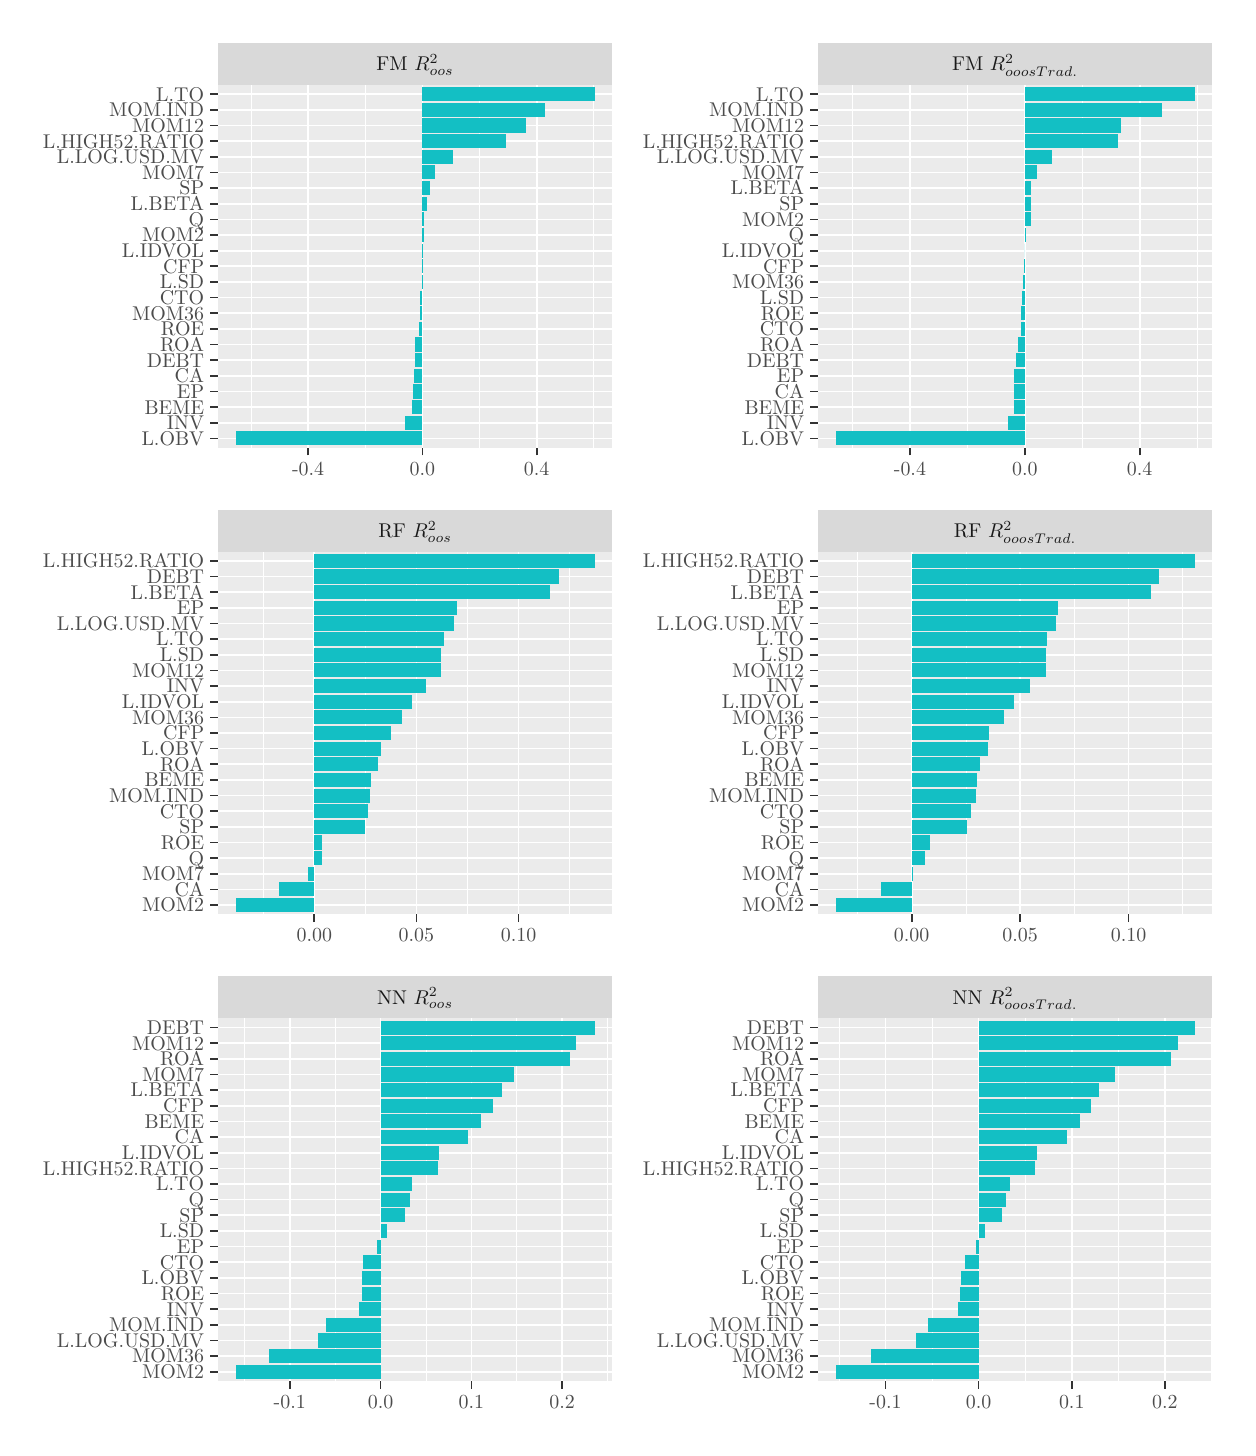
\begin{tikzpicture}[x=1pt,y=1pt]
\definecolor{fillColor}{RGB}{255,255,255}
\path[use as bounding box,fill=fillColor,fill opacity=0.00] (0,0) rectangle (433.62,505.89);
\begin{scope}
\path[clip] (  0.00,337.26) rectangle (216.81,505.89);
\definecolor{drawColor}{RGB}{255,255,255}
\definecolor{fillColor}{RGB}{255,255,255}

\path[draw=drawColor,line width= 0.6pt,line join=round,line cap=round,fill=fillColor] (  0.00,337.26) rectangle (216.81,505.89);
\end{scope}
\begin{scope}
\path[clip] ( 68.69,354.07) rectangle (211.31,485.23);
\definecolor{fillColor}{gray}{0.92}

\path[fill=fillColor] ( 68.69,354.07) rectangle (211.31,485.23);
\definecolor{drawColor}{RGB}{255,255,255}

\path[draw=drawColor,line width= 0.3pt,line join=round] ( 80.68,354.07) --
	( 80.68,485.23);

\path[draw=drawColor,line width= 0.3pt,line join=round] (121.99,354.07) --
	(121.99,485.23);

\path[draw=drawColor,line width= 0.3pt,line join=round] (163.29,354.07) --
	(163.29,485.23);

\path[draw=drawColor,line width= 0.3pt,line join=round] (204.59,354.07) --
	(204.59,485.23);

\path[draw=drawColor,line width= 0.6pt,line join=round] ( 68.69,357.46) --
	(211.31,357.46);

\path[draw=drawColor,line width= 0.6pt,line join=round] ( 68.69,363.11) --
	(211.31,363.11);

\path[draw=drawColor,line width= 0.6pt,line join=round] ( 68.69,368.77) --
	(211.31,368.77);

\path[draw=drawColor,line width= 0.6pt,line join=round] ( 68.69,374.42) --
	(211.31,374.42);

\path[draw=drawColor,line width= 0.6pt,line join=round] ( 68.69,380.07) --
	(211.31,380.07);

\path[draw=drawColor,line width= 0.6pt,line join=round] ( 68.69,385.73) --
	(211.31,385.73);

\path[draw=drawColor,line width= 0.6pt,line join=round] ( 68.69,391.38) --
	(211.31,391.38);

\path[draw=drawColor,line width= 0.6pt,line join=round] ( 68.69,397.04) --
	(211.31,397.04);

\path[draw=drawColor,line width= 0.6pt,line join=round] ( 68.69,402.69) --
	(211.31,402.69);

\path[draw=drawColor,line width= 0.6pt,line join=round] ( 68.69,408.34) --
	(211.31,408.34);

\path[draw=drawColor,line width= 0.6pt,line join=round] ( 68.69,414.00) --
	(211.31,414.00);

\path[draw=drawColor,line width= 0.6pt,line join=round] ( 68.69,419.65) --
	(211.31,419.65);

\path[draw=drawColor,line width= 0.6pt,line join=round] ( 68.69,425.30) --
	(211.31,425.30);

\path[draw=drawColor,line width= 0.6pt,line join=round] ( 68.69,430.96) --
	(211.31,430.96);

\path[draw=drawColor,line width= 0.6pt,line join=round] ( 68.69,436.61) --
	(211.31,436.61);

\path[draw=drawColor,line width= 0.6pt,line join=round] ( 68.69,442.26) --
	(211.31,442.26);

\path[draw=drawColor,line width= 0.6pt,line join=round] ( 68.69,447.92) --
	(211.31,447.92);

\path[draw=drawColor,line width= 0.6pt,line join=round] ( 68.69,453.57) --
	(211.31,453.57);

\path[draw=drawColor,line width= 0.6pt,line join=round] ( 68.69,459.23) --
	(211.31,459.23);

\path[draw=drawColor,line width= 0.6pt,line join=round] ( 68.69,464.88) --
	(211.31,464.88);

\path[draw=drawColor,line width= 0.6pt,line join=round] ( 68.69,470.53) --
	(211.31,470.53);

\path[draw=drawColor,line width= 0.6pt,line join=round] ( 68.69,476.19) --
	(211.31,476.19);

\path[draw=drawColor,line width= 0.6pt,line join=round] ( 68.69,481.84) --
	(211.31,481.84);

\path[draw=drawColor,line width= 0.6pt,line join=round] (101.34,354.07) --
	(101.34,485.23);

\path[draw=drawColor,line width= 0.6pt,line join=round] (142.64,354.07) --
	(142.64,485.23);

\path[draw=drawColor,line width= 0.6pt,line join=round] (183.94,354.07) --
	(183.94,485.23);
\definecolor{fillColor}{RGB}{19,191,196}

\path[fill=fillColor] (139.48,377.53) rectangle (142.64,382.62);

\path[fill=fillColor] (141.81,405.80) rectangle (142.64,410.89);

\path[fill=fillColor] (139.03,366.22) rectangle (142.64,371.31);

\path[fill=fillColor] (142.64,417.11) rectangle (142.82,422.19);

\path[fill=fillColor] (136.52,360.57) rectangle (142.64,365.66);

\path[fill=fillColor] (139.90,383.18) rectangle (142.64,388.27);

\path[fill=fillColor] (142.64,445.37) rectangle (145.48,450.46);

\path[fill=fillColor] (139.21,371.88) rectangle (142.64,376.97);

\path[fill=fillColor] (140.09,388.84) rectangle (142.64,393.93);

\path[fill=fillColor] (141.46,394.49) rectangle (142.64,399.58);

\path[fill=fillColor] (142.64,434.07) rectangle (143.28,439.15);

\path[fill=fillColor] (142.64,451.03) rectangle (147.18,456.12);

\path[fill=fillColor] (142.64,467.99) rectangle (180.01,473.08);

\path[fill=fillColor] (141.60,400.15) rectangle (142.64,405.23);

\path[fill=fillColor] (142.64,428.41) rectangle (143.08,433.50);

\path[fill=fillColor] (142.64,473.64) rectangle (186.98,478.73);

\path[fill=fillColor] (142.46,411.45) rectangle (142.64,416.54);

\path[fill=fillColor] (142.64,462.33) rectangle (172.88,467.42);

\path[fill=fillColor] (142.64,439.72) rectangle (144.15,444.81);

\path[fill=fillColor] (142.64,422.76) rectangle (142.88,427.85);

\path[fill=fillColor] (142.64,456.68) rectangle (153.67,461.77);

\path[fill=fillColor] (142.64,479.30) rectangle (204.83,484.38);

\path[fill=fillColor] ( 75.17,354.92) rectangle (142.64,360.00);
\end{scope}
\begin{scope}
\path[clip] ( 68.69,485.23) rectangle (211.31,500.39);
\definecolor{fillColor}{gray}{0.85}

\path[fill=fillColor] ( 68.69,485.23) rectangle (211.31,500.39);
\definecolor{drawColor}{gray}{0.10}

\node[text=drawColor,anchor=base,inner sep=0pt, outer sep=0pt, scale=  0.72] at (140.00,490.33) {FM $R^2_{oos}$};
\end{scope}
\begin{scope}
\path[clip] (  0.00,  0.00) rectangle (433.62,505.89);
\definecolor{drawColor}{gray}{0.20}

\path[draw=drawColor,line width= 0.6pt,line join=round] (101.34,351.32) --
	(101.34,354.07);

\path[draw=drawColor,line width= 0.6pt,line join=round] (142.64,351.32) --
	(142.64,354.07);

\path[draw=drawColor,line width= 0.6pt,line join=round] (183.94,351.32) --
	(183.94,354.07);
\end{scope}
\begin{scope}
\path[clip] (  0.00,  0.00) rectangle (433.62,505.89);
\definecolor{drawColor}{gray}{0.30}

\node[text=drawColor,anchor=base,inner sep=0pt, outer sep=0pt, scale=  0.72] at (101.34,344.16) {-0.4};

\node[text=drawColor,anchor=base,inner sep=0pt, outer sep=0pt, scale=  0.72] at (142.64,344.16) {0.0};

\node[text=drawColor,anchor=base,inner sep=0pt, outer sep=0pt, scale=  0.72] at (183.94,344.16) {0.4};
\end{scope}
\begin{scope}
\path[clip] (  0.00,  0.00) rectangle (433.62,505.89);
\definecolor{drawColor}{gray}{0.30}

\node[text=drawColor,anchor=base east,inner sep=0pt, outer sep=0pt, scale=  0.72] at ( 63.74,354.98) {L.OBV};

\node[text=drawColor,anchor=base east,inner sep=0pt, outer sep=0pt, scale=  0.72] at ( 63.74,360.63) {INV};

\node[text=drawColor,anchor=base east,inner sep=0pt, outer sep=0pt, scale=  0.72] at ( 63.74,366.29) {BEME};

\node[text=drawColor,anchor=base east,inner sep=0pt, outer sep=0pt, scale=  0.72] at ( 63.74,371.94) {EP};

\node[text=drawColor,anchor=base east,inner sep=0pt, outer sep=0pt, scale=  0.72] at ( 63.74,377.60) {CA};

\node[text=drawColor,anchor=base east,inner sep=0pt, outer sep=0pt, scale=  0.72] at ( 63.74,383.25) {DEBT};

\node[text=drawColor,anchor=base east,inner sep=0pt, outer sep=0pt, scale=  0.72] at ( 63.74,388.90) {ROA};

\node[text=drawColor,anchor=base east,inner sep=0pt, outer sep=0pt, scale=  0.72] at ( 63.74,394.56) {ROE};

\node[text=drawColor,anchor=base east,inner sep=0pt, outer sep=0pt, scale=  0.72] at ( 63.74,400.21) {MOM36};

\node[text=drawColor,anchor=base east,inner sep=0pt, outer sep=0pt, scale=  0.72] at ( 63.74,405.86) {CTO};

\node[text=drawColor,anchor=base east,inner sep=0pt, outer sep=0pt, scale=  0.72] at ( 63.74,411.52) {L.SD};

\node[text=drawColor,anchor=base east,inner sep=0pt, outer sep=0pt, scale=  0.72] at ( 63.74,417.17) {CFP};

\node[text=drawColor,anchor=base east,inner sep=0pt, outer sep=0pt, scale=  0.72] at ( 63.74,422.82) {L.IDVOL};

\node[text=drawColor,anchor=base east,inner sep=0pt, outer sep=0pt, scale=  0.72] at ( 63.74,428.48) {MOM2};

\node[text=drawColor,anchor=base east,inner sep=0pt, outer sep=0pt, scale=  0.72] at ( 63.74,434.13) {Q};

\node[text=drawColor,anchor=base east,inner sep=0pt, outer sep=0pt, scale=  0.72] at ( 63.74,439.78) {L.BETA};

\node[text=drawColor,anchor=base east,inner sep=0pt, outer sep=0pt, scale=  0.72] at ( 63.74,445.44) {SP};

\node[text=drawColor,anchor=base east,inner sep=0pt, outer sep=0pt, scale=  0.72] at ( 63.74,451.09) {MOM7};

\node[text=drawColor,anchor=base east,inner sep=0pt, outer sep=0pt, scale=  0.72] at ( 63.74,456.75) {L.LOG.USD.MV};

\node[text=drawColor,anchor=base east,inner sep=0pt, outer sep=0pt, scale=  0.72] at ( 63.74,462.40) {L.HIGH52.RATIO};

\node[text=drawColor,anchor=base east,inner sep=0pt, outer sep=0pt, scale=  0.72] at ( 63.74,468.05) {MOM12};

\node[text=drawColor,anchor=base east,inner sep=0pt, outer sep=0pt, scale=  0.72] at ( 63.74,473.71) {MOM.IND};

\node[text=drawColor,anchor=base east,inner sep=0pt, outer sep=0pt, scale=  0.72] at ( 63.74,479.36) {L.TO};
\end{scope}
\begin{scope}
\path[clip] (  0.00,  0.00) rectangle (433.62,505.89);
\definecolor{drawColor}{gray}{0.20}

\path[draw=drawColor,line width= 0.6pt,line join=round] ( 65.94,357.46) --
	( 68.69,357.46);

\path[draw=drawColor,line width= 0.6pt,line join=round] ( 65.94,363.11) --
	( 68.69,363.11);

\path[draw=drawColor,line width= 0.6pt,line join=round] ( 65.94,368.77) --
	( 68.69,368.77);

\path[draw=drawColor,line width= 0.6pt,line join=round] ( 65.94,374.42) --
	( 68.69,374.42);

\path[draw=drawColor,line width= 0.6pt,line join=round] ( 65.94,380.07) --
	( 68.69,380.07);

\path[draw=drawColor,line width= 0.6pt,line join=round] ( 65.94,385.73) --
	( 68.69,385.73);

\path[draw=drawColor,line width= 0.6pt,line join=round] ( 65.94,391.38) --
	( 68.69,391.38);

\path[draw=drawColor,line width= 0.6pt,line join=round] ( 65.94,397.04) --
	( 68.69,397.04);

\path[draw=drawColor,line width= 0.6pt,line join=round] ( 65.94,402.69) --
	( 68.69,402.69);

\path[draw=drawColor,line width= 0.6pt,line join=round] ( 65.94,408.34) --
	( 68.69,408.34);

\path[draw=drawColor,line width= 0.6pt,line join=round] ( 65.94,414.00) --
	( 68.69,414.00);

\path[draw=drawColor,line width= 0.6pt,line join=round] ( 65.94,419.65) --
	( 68.69,419.65);

\path[draw=drawColor,line width= 0.6pt,line join=round] ( 65.94,425.30) --
	( 68.69,425.30);

\path[draw=drawColor,line width= 0.6pt,line join=round] ( 65.94,430.96) --
	( 68.69,430.96);

\path[draw=drawColor,line width= 0.6pt,line join=round] ( 65.94,436.61) --
	( 68.69,436.61);

\path[draw=drawColor,line width= 0.6pt,line join=round] ( 65.94,442.26) --
	( 68.69,442.26);

\path[draw=drawColor,line width= 0.6pt,line join=round] ( 65.94,447.92) --
	( 68.69,447.92);

\path[draw=drawColor,line width= 0.6pt,line join=round] ( 65.94,453.57) --
	( 68.69,453.57);

\path[draw=drawColor,line width= 0.6pt,line join=round] ( 65.94,459.23) --
	( 68.69,459.23);

\path[draw=drawColor,line width= 0.6pt,line join=round] ( 65.94,464.88) --
	( 68.69,464.88);

\path[draw=drawColor,line width= 0.6pt,line join=round] ( 65.94,470.53) --
	( 68.69,470.53);

\path[draw=drawColor,line width= 0.6pt,line join=round] ( 65.94,476.19) --
	( 68.69,476.19);

\path[draw=drawColor,line width= 0.6pt,line join=round] ( 65.94,481.84) --
	( 68.69,481.84);
\end{scope}
\begin{scope}
\path[clip] (216.81,337.26) rectangle (433.62,505.89);
\definecolor{drawColor}{RGB}{255,255,255}
\definecolor{fillColor}{RGB}{255,255,255}

\path[draw=drawColor,line width= 0.6pt,line join=round,line cap=round,fill=fillColor] (216.81,337.26) rectangle (433.62,505.89);
\end{scope}
\begin{scope}
\path[clip] (285.50,354.07) rectangle (428.12,485.23);
\definecolor{fillColor}{gray}{0.92}

\path[fill=fillColor] (285.50,354.07) rectangle (428.12,485.23);
\definecolor{drawColor}{RGB}{255,255,255}

\path[draw=drawColor,line width= 0.3pt,line join=round] (298.05,354.07) --
	(298.05,485.23);

\path[draw=drawColor,line width= 0.3pt,line join=round] (339.56,354.07) --
	(339.56,485.23);

\path[draw=drawColor,line width= 0.3pt,line join=round] (381.06,354.07) --
	(381.06,485.23);

\path[draw=drawColor,line width= 0.3pt,line join=round] (422.57,354.07) --
	(422.57,485.23);

\path[draw=drawColor,line width= 0.6pt,line join=round] (285.50,357.46) --
	(428.12,357.46);

\path[draw=drawColor,line width= 0.6pt,line join=round] (285.50,363.11) --
	(428.12,363.11);

\path[draw=drawColor,line width= 0.6pt,line join=round] (285.50,368.77) --
	(428.12,368.77);

\path[draw=drawColor,line width= 0.6pt,line join=round] (285.50,374.42) --
	(428.12,374.42);

\path[draw=drawColor,line width= 0.6pt,line join=round] (285.50,380.07) --
	(428.12,380.07);

\path[draw=drawColor,line width= 0.6pt,line join=round] (285.50,385.73) --
	(428.12,385.73);

\path[draw=drawColor,line width= 0.6pt,line join=round] (285.50,391.38) --
	(428.12,391.38);

\path[draw=drawColor,line width= 0.6pt,line join=round] (285.50,397.04) --
	(428.12,397.04);

\path[draw=drawColor,line width= 0.6pt,line join=round] (285.50,402.69) --
	(428.12,402.69);

\path[draw=drawColor,line width= 0.6pt,line join=round] (285.50,408.34) --
	(428.12,408.34);

\path[draw=drawColor,line width= 0.6pt,line join=round] (285.50,414.00) --
	(428.12,414.00);

\path[draw=drawColor,line width= 0.6pt,line join=round] (285.50,419.65) --
	(428.12,419.65);

\path[draw=drawColor,line width= 0.6pt,line join=round] (285.50,425.30) --
	(428.12,425.30);

\path[draw=drawColor,line width= 0.6pt,line join=round] (285.50,430.96) --
	(428.12,430.96);

\path[draw=drawColor,line width= 0.6pt,line join=round] (285.50,436.61) --
	(428.12,436.61);

\path[draw=drawColor,line width= 0.6pt,line join=round] (285.50,442.26) --
	(428.12,442.26);

\path[draw=drawColor,line width= 0.6pt,line join=round] (285.50,447.92) --
	(428.12,447.92);

\path[draw=drawColor,line width= 0.6pt,line join=round] (285.50,453.57) --
	(428.12,453.57);

\path[draw=drawColor,line width= 0.6pt,line join=round] (285.50,459.23) --
	(428.12,459.23);

\path[draw=drawColor,line width= 0.6pt,line join=round] (285.50,464.88) --
	(428.12,464.88);

\path[draw=drawColor,line width= 0.6pt,line join=round] (285.50,470.53) --
	(428.12,470.53);

\path[draw=drawColor,line width= 0.6pt,line join=round] (285.50,476.19) --
	(428.12,476.19);

\path[draw=drawColor,line width= 0.6pt,line join=round] (285.50,481.84) --
	(428.12,481.84);

\path[draw=drawColor,line width= 0.6pt,line join=round] (318.80,354.07) --
	(318.80,485.23);

\path[draw=drawColor,line width= 0.6pt,line join=round] (360.31,354.07) --
	(360.31,485.23);

\path[draw=drawColor,line width= 0.6pt,line join=round] (401.82,354.07) --
	(401.82,485.23);
\definecolor{fillColor}{RGB}{19,191,196}

\path[fill=fillColor] (356.44,371.88) rectangle (360.31,376.97);

\path[fill=fillColor] (358.85,394.49) rectangle (360.31,399.58);

\path[fill=fillColor] (356.41,366.22) rectangle (360.31,371.31);

\path[fill=fillColor] (360.16,417.11) rectangle (360.31,422.19);

\path[fill=fillColor] (354.11,360.57) rectangle (360.31,365.66);

\path[fill=fillColor] (357.09,383.18) rectangle (360.31,388.27);

\path[fill=fillColor] (360.31,439.72) rectangle (362.56,444.81);

\path[fill=fillColor] (356.58,377.53) rectangle (360.31,382.62);

\path[fill=fillColor] (357.68,388.84) rectangle (360.31,393.93);

\path[fill=fillColor] (358.95,400.15) rectangle (360.31,405.23);

\path[fill=fillColor] (360.31,428.41) rectangle (360.61,433.50);

\path[fill=fillColor] (360.31,451.03) rectangle (364.60,456.12);

\path[fill=fillColor] (360.31,467.99) rectangle (395.13,473.08);

\path[fill=fillColor] (359.53,411.45) rectangle (360.31,416.54);

\path[fill=fillColor] (360.31,434.07) rectangle (362.37,439.15);

\path[fill=fillColor] (360.31,473.64) rectangle (409.92,478.73);

\path[fill=fillColor] (359.19,405.80) rectangle (360.31,410.89);

\path[fill=fillColor] (360.31,462.33) rectangle (394.12,467.42);

\path[fill=fillColor] (360.31,445.37) rectangle (362.61,450.46);

\path[fill=fillColor] (360.31,422.76) rectangle (360.31,427.85);

\path[fill=fillColor] (360.31,456.68) rectangle (370.08,461.77);

\path[fill=fillColor] (360.31,479.30) rectangle (421.64,484.38);

\path[fill=fillColor] (291.98,354.92) rectangle (360.31,360.00);
\end{scope}
\begin{scope}
\path[clip] (285.50,485.23) rectangle (428.12,500.39);
\definecolor{fillColor}{gray}{0.85}

\path[fill=fillColor] (285.50,485.23) rectangle (428.12,500.39);
\definecolor{drawColor}{gray}{0.10}

\node[text=drawColor,anchor=base,inner sep=0pt, outer sep=0pt, scale=  0.72] at (356.81,490.33) {FM $R^2_{ooos  Trad.}$};
\end{scope}
\begin{scope}
\path[clip] (  0.00,  0.00) rectangle (433.62,505.89);
\definecolor{drawColor}{gray}{0.20}

\path[draw=drawColor,line width= 0.6pt,line join=round] (318.80,351.32) --
	(318.80,354.07);

\path[draw=drawColor,line width= 0.6pt,line join=round] (360.31,351.32) --
	(360.31,354.07);

\path[draw=drawColor,line width= 0.6pt,line join=round] (401.82,351.32) --
	(401.82,354.07);
\end{scope}
\begin{scope}
\path[clip] (  0.00,  0.00) rectangle (433.62,505.89);
\definecolor{drawColor}{gray}{0.30}

\node[text=drawColor,anchor=base,inner sep=0pt, outer sep=0pt, scale=  0.72] at (318.80,344.16) {-0.4};

\node[text=drawColor,anchor=base,inner sep=0pt, outer sep=0pt, scale=  0.72] at (360.31,344.16) {0.0};

\node[text=drawColor,anchor=base,inner sep=0pt, outer sep=0pt, scale=  0.72] at (401.82,344.16) {0.4};
\end{scope}
\begin{scope}
\path[clip] (  0.00,  0.00) rectangle (433.62,505.89);
\definecolor{drawColor}{gray}{0.30}

\node[text=drawColor,anchor=base east,inner sep=0pt, outer sep=0pt, scale=  0.72] at (280.55,354.98) {L.OBV};

\node[text=drawColor,anchor=base east,inner sep=0pt, outer sep=0pt, scale=  0.72] at (280.55,360.63) {INV};

\node[text=drawColor,anchor=base east,inner sep=0pt, outer sep=0pt, scale=  0.72] at (280.55,366.29) {BEME};

\node[text=drawColor,anchor=base east,inner sep=0pt, outer sep=0pt, scale=  0.72] at (280.55,371.94) {CA};

\node[text=drawColor,anchor=base east,inner sep=0pt, outer sep=0pt, scale=  0.72] at (280.55,377.60) {EP};

\node[text=drawColor,anchor=base east,inner sep=0pt, outer sep=0pt, scale=  0.72] at (280.55,383.25) {DEBT};

\node[text=drawColor,anchor=base east,inner sep=0pt, outer sep=0pt, scale=  0.72] at (280.55,388.90) {ROA};

\node[text=drawColor,anchor=base east,inner sep=0pt, outer sep=0pt, scale=  0.72] at (280.55,394.56) {CTO};

\node[text=drawColor,anchor=base east,inner sep=0pt, outer sep=0pt, scale=  0.72] at (280.55,400.21) {ROE};

\node[text=drawColor,anchor=base east,inner sep=0pt, outer sep=0pt, scale=  0.72] at (280.55,405.86) {L.SD};

\node[text=drawColor,anchor=base east,inner sep=0pt, outer sep=0pt, scale=  0.72] at (280.55,411.52) {MOM36};

\node[text=drawColor,anchor=base east,inner sep=0pt, outer sep=0pt, scale=  0.72] at (280.55,417.17) {CFP};

\node[text=drawColor,anchor=base east,inner sep=0pt, outer sep=0pt, scale=  0.72] at (280.55,422.82) {L.IDVOL};

\node[text=drawColor,anchor=base east,inner sep=0pt, outer sep=0pt, scale=  0.72] at (280.55,428.48) {Q};

\node[text=drawColor,anchor=base east,inner sep=0pt, outer sep=0pt, scale=  0.72] at (280.55,434.13) {MOM2};

\node[text=drawColor,anchor=base east,inner sep=0pt, outer sep=0pt, scale=  0.72] at (280.55,439.78) {SP};

\node[text=drawColor,anchor=base east,inner sep=0pt, outer sep=0pt, scale=  0.72] at (280.55,445.44) {L.BETA};

\node[text=drawColor,anchor=base east,inner sep=0pt, outer sep=0pt, scale=  0.72] at (280.55,451.09) {MOM7};

\node[text=drawColor,anchor=base east,inner sep=0pt, outer sep=0pt, scale=  0.72] at (280.55,456.75) {L.LOG.USD.MV};

\node[text=drawColor,anchor=base east,inner sep=0pt, outer sep=0pt, scale=  0.72] at (280.55,462.40) {L.HIGH52.RATIO};

\node[text=drawColor,anchor=base east,inner sep=0pt, outer sep=0pt, scale=  0.72] at (280.55,468.05) {MOM12};

\node[text=drawColor,anchor=base east,inner sep=0pt, outer sep=0pt, scale=  0.72] at (280.55,473.71) {MOM.IND};

\node[text=drawColor,anchor=base east,inner sep=0pt, outer sep=0pt, scale=  0.72] at (280.55,479.36) {L.TO};
\end{scope}
\begin{scope}
\path[clip] (  0.00,  0.00) rectangle (433.62,505.89);
\definecolor{drawColor}{gray}{0.20}

\path[draw=drawColor,line width= 0.6pt,line join=round] (282.75,357.46) --
	(285.50,357.46);

\path[draw=drawColor,line width= 0.6pt,line join=round] (282.75,363.11) --
	(285.50,363.11);

\path[draw=drawColor,line width= 0.6pt,line join=round] (282.75,368.77) --
	(285.50,368.77);

\path[draw=drawColor,line width= 0.6pt,line join=round] (282.75,374.42) --
	(285.50,374.42);

\path[draw=drawColor,line width= 0.6pt,line join=round] (282.75,380.07) --
	(285.50,380.07);

\path[draw=drawColor,line width= 0.6pt,line join=round] (282.75,385.73) --
	(285.50,385.73);

\path[draw=drawColor,line width= 0.6pt,line join=round] (282.75,391.38) --
	(285.50,391.38);

\path[draw=drawColor,line width= 0.6pt,line join=round] (282.75,397.04) --
	(285.50,397.04);

\path[draw=drawColor,line width= 0.6pt,line join=round] (282.75,402.69) --
	(285.50,402.69);

\path[draw=drawColor,line width= 0.6pt,line join=round] (282.75,408.34) --
	(285.50,408.34);

\path[draw=drawColor,line width= 0.6pt,line join=round] (282.75,414.00) --
	(285.50,414.00);

\path[draw=drawColor,line width= 0.6pt,line join=round] (282.75,419.65) --
	(285.50,419.65);

\path[draw=drawColor,line width= 0.6pt,line join=round] (282.75,425.30) --
	(285.50,425.30);

\path[draw=drawColor,line width= 0.6pt,line join=round] (282.75,430.96) --
	(285.50,430.96);

\path[draw=drawColor,line width= 0.6pt,line join=round] (282.75,436.61) --
	(285.50,436.61);

\path[draw=drawColor,line width= 0.6pt,line join=round] (282.75,442.26) --
	(285.50,442.26);

\path[draw=drawColor,line width= 0.6pt,line join=round] (282.75,447.92) --
	(285.50,447.92);

\path[draw=drawColor,line width= 0.6pt,line join=round] (282.75,453.57) --
	(285.50,453.57);

\path[draw=drawColor,line width= 0.6pt,line join=round] (282.75,459.23) --
	(285.50,459.23);

\path[draw=drawColor,line width= 0.6pt,line join=round] (282.75,464.88) --
	(285.50,464.88);

\path[draw=drawColor,line width= 0.6pt,line join=round] (282.75,470.53) --
	(285.50,470.53);

\path[draw=drawColor,line width= 0.6pt,line join=round] (282.75,476.19) --
	(285.50,476.19);

\path[draw=drawColor,line width= 0.6pt,line join=round] (282.75,481.84) --
	(285.50,481.84);
\end{scope}
\begin{scope}
\path[clip] (  0.00,168.63) rectangle (216.81,337.26);
\definecolor{drawColor}{RGB}{255,255,255}
\definecolor{fillColor}{RGB}{255,255,255}

\path[draw=drawColor,line width= 0.6pt,line join=round,line cap=round,fill=fillColor] (  0.00,168.63) rectangle (216.81,337.26);
\end{scope}
\begin{scope}
\path[clip] ( 68.69,185.44) rectangle (211.31,316.60);
\definecolor{fillColor}{gray}{0.92}

\path[fill=fillColor] ( 68.69,185.44) rectangle (211.31,316.60);
\definecolor{drawColor}{RGB}{255,255,255}

\path[draw=drawColor,line width= 0.3pt,line join=round] ( 85.10,185.44) --
	( 85.10,316.60);

\path[draw=drawColor,line width= 0.3pt,line join=round] (122.01,185.44) --
	(122.01,316.60);

\path[draw=drawColor,line width= 0.3pt,line join=round] (158.92,185.44) --
	(158.92,316.60);

\path[draw=drawColor,line width= 0.3pt,line join=round] (195.83,185.44) --
	(195.83,316.60);

\path[draw=drawColor,line width= 0.6pt,line join=round] ( 68.69,188.83) --
	(211.31,188.83);

\path[draw=drawColor,line width= 0.6pt,line join=round] ( 68.69,194.48) --
	(211.31,194.48);

\path[draw=drawColor,line width= 0.6pt,line join=round] ( 68.69,200.14) --
	(211.31,200.14);

\path[draw=drawColor,line width= 0.6pt,line join=round] ( 68.69,205.79) --
	(211.31,205.79);

\path[draw=drawColor,line width= 0.6pt,line join=round] ( 68.69,211.44) --
	(211.31,211.44);

\path[draw=drawColor,line width= 0.6pt,line join=round] ( 68.69,217.10) --
	(211.31,217.10);

\path[draw=drawColor,line width= 0.6pt,line join=round] ( 68.69,222.75) --
	(211.31,222.75);

\path[draw=drawColor,line width= 0.6pt,line join=round] ( 68.69,228.41) --
	(211.31,228.41);

\path[draw=drawColor,line width= 0.6pt,line join=round] ( 68.69,234.06) --
	(211.31,234.06);

\path[draw=drawColor,line width= 0.6pt,line join=round] ( 68.69,239.71) --
	(211.31,239.71);

\path[draw=drawColor,line width= 0.6pt,line join=round] ( 68.69,245.37) --
	(211.31,245.37);

\path[draw=drawColor,line width= 0.6pt,line join=round] ( 68.69,251.02) --
	(211.31,251.02);

\path[draw=drawColor,line width= 0.6pt,line join=round] ( 68.69,256.67) --
	(211.31,256.67);

\path[draw=drawColor,line width= 0.6pt,line join=round] ( 68.69,262.33) --
	(211.31,262.33);

\path[draw=drawColor,line width= 0.6pt,line join=round] ( 68.69,267.98) --
	(211.31,267.98);

\path[draw=drawColor,line width= 0.6pt,line join=round] ( 68.69,273.63) --
	(211.31,273.63);

\path[draw=drawColor,line width= 0.6pt,line join=round] ( 68.69,279.29) --
	(211.31,279.29);

\path[draw=drawColor,line width= 0.6pt,line join=round] ( 68.69,284.94) --
	(211.31,284.94);

\path[draw=drawColor,line width= 0.6pt,line join=round] ( 68.69,290.60) --
	(211.31,290.60);

\path[draw=drawColor,line width= 0.6pt,line join=round] ( 68.69,296.25) --
	(211.31,296.25);

\path[draw=drawColor,line width= 0.6pt,line join=round] ( 68.69,301.90) --
	(211.31,301.90);

\path[draw=drawColor,line width= 0.6pt,line join=round] ( 68.69,307.56) --
	(211.31,307.56);

\path[draw=drawColor,line width= 0.6pt,line join=round] ( 68.69,313.21) --
	(211.31,313.21);

\path[draw=drawColor,line width= 0.6pt,line join=round] (103.56,185.44) --
	(103.56,316.60);

\path[draw=drawColor,line width= 0.6pt,line join=round] (140.46,185.44) --
	(140.46,316.60);

\path[draw=drawColor,line width= 0.6pt,line join=round] (177.37,185.44) --
	(177.37,316.60);
\definecolor{fillColor}{RGB}{19,191,196}

\path[fill=fillColor] ( 90.75,191.94) rectangle (103.56,197.03);

\path[fill=fillColor] (103.56,220.21) rectangle (123.12,225.30);

\path[fill=fillColor] (103.56,231.52) rectangle (124.13,236.60);

\path[fill=fillColor] (103.56,248.48) rectangle (131.46,253.56);

\path[fill=fillColor] (103.56,265.44) rectangle (144.06,270.52);

\path[fill=fillColor] (103.56,305.01) rectangle (191.83,310.10);

\path[fill=fillColor] (103.56,214.55) rectangle (121.72,219.64);

\path[fill=fillColor] (103.56,293.70) rectangle (154.96,298.79);

\path[fill=fillColor] (103.56,237.17) rectangle (126.48,242.26);

\path[fill=fillColor] (103.56,208.90) rectangle (106.28,213.99);

\path[fill=fillColor] (103.56,203.25) rectangle (106.25,208.34);

\path[fill=fillColor] (101.32,197.59) rectangle (103.56,202.68);

\path[fill=fillColor] (103.56,271.09) rectangle (149.38,276.18);

\path[fill=fillColor] (103.56,254.13) rectangle (135.27,259.22);

\path[fill=fillColor] ( 75.17,186.29) rectangle (103.56,191.37);

\path[fill=fillColor] (103.56,225.86) rectangle (123.68,230.95);

\path[fill=fillColor] (103.56,276.74) rectangle (149.52,281.83);

\path[fill=fillColor] (103.56,310.67) rectangle (204.83,315.75);

\path[fill=fillColor] (103.56,299.36) rectangle (188.83,304.45);

\path[fill=fillColor] (103.56,259.78) rectangle (138.82,264.87);

\path[fill=fillColor] (103.56,288.05) rectangle (154.05,293.14);

\path[fill=fillColor] (103.56,282.40) rectangle (150.34,287.49);

\path[fill=fillColor] (103.56,242.82) rectangle (127.72,247.91);
\end{scope}
\begin{scope}
\path[clip] ( 68.69,316.60) rectangle (211.31,331.76);
\definecolor{fillColor}{gray}{0.85}

\path[fill=fillColor] ( 68.69,316.60) rectangle (211.31,331.76);
\definecolor{drawColor}{gray}{0.10}

\node[text=drawColor,anchor=base,inner sep=0pt, outer sep=0pt, scale=  0.72] at (140.00,321.70) {RF $R^2_{oos}$};
\end{scope}
\begin{scope}
\path[clip] (  0.00,  0.00) rectangle (433.62,505.89);
\definecolor{drawColor}{gray}{0.20}

\path[draw=drawColor,line width= 0.6pt,line join=round] (103.56,182.69) --
	(103.56,185.44);

\path[draw=drawColor,line width= 0.6pt,line join=round] (140.46,182.69) --
	(140.46,185.44);

\path[draw=drawColor,line width= 0.6pt,line join=round] (177.37,182.69) --
	(177.37,185.44);
\end{scope}
\begin{scope}
\path[clip] (  0.00,  0.00) rectangle (433.62,505.89);
\definecolor{drawColor}{gray}{0.30}

\node[text=drawColor,anchor=base,inner sep=0pt, outer sep=0pt, scale=  0.72] at (103.56,175.53) {0.00};

\node[text=drawColor,anchor=base,inner sep=0pt, outer sep=0pt, scale=  0.72] at (140.46,175.53) {0.05};

\node[text=drawColor,anchor=base,inner sep=0pt, outer sep=0pt, scale=  0.72] at (177.37,175.53) {0.10};
\end{scope}
\begin{scope}
\path[clip] (  0.00,  0.00) rectangle (433.62,505.89);
\definecolor{drawColor}{gray}{0.30}

\node[text=drawColor,anchor=base east,inner sep=0pt, outer sep=0pt, scale=  0.72] at ( 63.74,186.35) {MOM2};

\node[text=drawColor,anchor=base east,inner sep=0pt, outer sep=0pt, scale=  0.72] at ( 63.74,192.00) {CA};

\node[text=drawColor,anchor=base east,inner sep=0pt, outer sep=0pt, scale=  0.72] at ( 63.74,197.66) {MOM7};

\node[text=drawColor,anchor=base east,inner sep=0pt, outer sep=0pt, scale=  0.72] at ( 63.74,203.31) {Q};

\node[text=drawColor,anchor=base east,inner sep=0pt, outer sep=0pt, scale=  0.72] at ( 63.74,208.97) {ROE};

\node[text=drawColor,anchor=base east,inner sep=0pt, outer sep=0pt, scale=  0.72] at ( 63.74,214.62) {SP};

\node[text=drawColor,anchor=base east,inner sep=0pt, outer sep=0pt, scale=  0.72] at ( 63.74,220.27) {CTO};

\node[text=drawColor,anchor=base east,inner sep=0pt, outer sep=0pt, scale=  0.72] at ( 63.74,225.93) {MOM.IND};

\node[text=drawColor,anchor=base east,inner sep=0pt, outer sep=0pt, scale=  0.72] at ( 63.74,231.58) {BEME};

\node[text=drawColor,anchor=base east,inner sep=0pt, outer sep=0pt, scale=  0.72] at ( 63.74,237.23) {ROA};

\node[text=drawColor,anchor=base east,inner sep=0pt, outer sep=0pt, scale=  0.72] at ( 63.74,242.89) {L.OBV};

\node[text=drawColor,anchor=base east,inner sep=0pt, outer sep=0pt, scale=  0.72] at ( 63.74,248.54) {CFP};

\node[text=drawColor,anchor=base east,inner sep=0pt, outer sep=0pt, scale=  0.72] at ( 63.74,254.19) {MOM36};

\node[text=drawColor,anchor=base east,inner sep=0pt, outer sep=0pt, scale=  0.72] at ( 63.74,259.85) {L.IDVOL};

\node[text=drawColor,anchor=base east,inner sep=0pt, outer sep=0pt, scale=  0.72] at ( 63.74,265.50) {INV};

\node[text=drawColor,anchor=base east,inner sep=0pt, outer sep=0pt, scale=  0.72] at ( 63.74,271.15) {MOM12};

\node[text=drawColor,anchor=base east,inner sep=0pt, outer sep=0pt, scale=  0.72] at ( 63.74,276.81) {L.SD};

\node[text=drawColor,anchor=base east,inner sep=0pt, outer sep=0pt, scale=  0.72] at ( 63.74,282.46) {L.TO};

\node[text=drawColor,anchor=base east,inner sep=0pt, outer sep=0pt, scale=  0.72] at ( 63.74,288.12) {L.LOG.USD.MV};

\node[text=drawColor,anchor=base east,inner sep=0pt, outer sep=0pt, scale=  0.72] at ( 63.74,293.77) {EP};

\node[text=drawColor,anchor=base east,inner sep=0pt, outer sep=0pt, scale=  0.72] at ( 63.74,299.42) {L.BETA};

\node[text=drawColor,anchor=base east,inner sep=0pt, outer sep=0pt, scale=  0.72] at ( 63.74,305.08) {DEBT};

\node[text=drawColor,anchor=base east,inner sep=0pt, outer sep=0pt, scale=  0.72] at ( 63.74,310.73) {L.HIGH52.RATIO};
\end{scope}
\begin{scope}
\path[clip] (  0.00,  0.00) rectangle (433.62,505.89);
\definecolor{drawColor}{gray}{0.20}

\path[draw=drawColor,line width= 0.6pt,line join=round] ( 65.94,188.83) --
	( 68.69,188.83);

\path[draw=drawColor,line width= 0.6pt,line join=round] ( 65.94,194.48) --
	( 68.69,194.48);

\path[draw=drawColor,line width= 0.6pt,line join=round] ( 65.94,200.14) --
	( 68.69,200.14);

\path[draw=drawColor,line width= 0.6pt,line join=round] ( 65.94,205.79) --
	( 68.69,205.79);

\path[draw=drawColor,line width= 0.6pt,line join=round] ( 65.94,211.44) --
	( 68.69,211.44);

\path[draw=drawColor,line width= 0.6pt,line join=round] ( 65.94,217.10) --
	( 68.69,217.10);

\path[draw=drawColor,line width= 0.6pt,line join=round] ( 65.94,222.75) --
	( 68.69,222.75);

\path[draw=drawColor,line width= 0.6pt,line join=round] ( 65.94,228.41) --
	( 68.69,228.41);

\path[draw=drawColor,line width= 0.6pt,line join=round] ( 65.94,234.06) --
	( 68.69,234.06);

\path[draw=drawColor,line width= 0.6pt,line join=round] ( 65.94,239.71) --
	( 68.69,239.71);

\path[draw=drawColor,line width= 0.6pt,line join=round] ( 65.94,245.37) --
	( 68.69,245.37);

\path[draw=drawColor,line width= 0.6pt,line join=round] ( 65.94,251.02) --
	( 68.69,251.02);

\path[draw=drawColor,line width= 0.6pt,line join=round] ( 65.94,256.67) --
	( 68.69,256.67);

\path[draw=drawColor,line width= 0.6pt,line join=round] ( 65.94,262.33) --
	( 68.69,262.33);

\path[draw=drawColor,line width= 0.6pt,line join=round] ( 65.94,267.98) --
	( 68.69,267.98);

\path[draw=drawColor,line width= 0.6pt,line join=round] ( 65.94,273.63) --
	( 68.69,273.63);

\path[draw=drawColor,line width= 0.6pt,line join=round] ( 65.94,279.29) --
	( 68.69,279.29);

\path[draw=drawColor,line width= 0.6pt,line join=round] ( 65.94,284.94) --
	( 68.69,284.94);

\path[draw=drawColor,line width= 0.6pt,line join=round] ( 65.94,290.60) --
	( 68.69,290.60);

\path[draw=drawColor,line width= 0.6pt,line join=round] ( 65.94,296.25) --
	( 68.69,296.25);

\path[draw=drawColor,line width= 0.6pt,line join=round] ( 65.94,301.90) --
	( 68.69,301.90);

\path[draw=drawColor,line width= 0.6pt,line join=round] ( 65.94,307.56) --
	( 68.69,307.56);

\path[draw=drawColor,line width= 0.6pt,line join=round] ( 65.94,313.21) --
	( 68.69,313.21);
\end{scope}
\begin{scope}
\path[clip] (216.81,168.63) rectangle (433.62,337.26);
\definecolor{drawColor}{RGB}{255,255,255}
\definecolor{fillColor}{RGB}{255,255,255}

\path[draw=drawColor,line width= 0.6pt,line join=round,line cap=round,fill=fillColor] (216.81,168.63) rectangle (433.62,337.26);
\end{scope}
\begin{scope}
\path[clip] (285.50,185.44) rectangle (428.12,316.60);
\definecolor{fillColor}{gray}{0.92}

\path[fill=fillColor] (285.50,185.44) rectangle (428.12,316.60);
\definecolor{drawColor}{RGB}{255,255,255}

\path[draw=drawColor,line width= 0.3pt,line join=round] (299.85,185.44) --
	(299.85,316.60);

\path[draw=drawColor,line width= 0.3pt,line join=round] (339.03,185.44) --
	(339.03,316.60);

\path[draw=drawColor,line width= 0.3pt,line join=round] (378.21,185.44) --
	(378.21,316.60);

\path[draw=drawColor,line width= 0.3pt,line join=round] (417.40,185.44) --
	(417.40,316.60);

\path[draw=drawColor,line width= 0.6pt,line join=round] (285.50,188.83) --
	(428.12,188.83);

\path[draw=drawColor,line width= 0.6pt,line join=round] (285.50,194.48) --
	(428.12,194.48);

\path[draw=drawColor,line width= 0.6pt,line join=round] (285.50,200.14) --
	(428.12,200.14);

\path[draw=drawColor,line width= 0.6pt,line join=round] (285.50,205.79) --
	(428.12,205.79);

\path[draw=drawColor,line width= 0.6pt,line join=round] (285.50,211.44) --
	(428.12,211.44);

\path[draw=drawColor,line width= 0.6pt,line join=round] (285.50,217.10) --
	(428.12,217.10);

\path[draw=drawColor,line width= 0.6pt,line join=round] (285.50,222.75) --
	(428.12,222.75);

\path[draw=drawColor,line width= 0.6pt,line join=round] (285.50,228.41) --
	(428.12,228.41);

\path[draw=drawColor,line width= 0.6pt,line join=round] (285.50,234.06) --
	(428.12,234.06);

\path[draw=drawColor,line width= 0.6pt,line join=round] (285.50,239.71) --
	(428.12,239.71);

\path[draw=drawColor,line width= 0.6pt,line join=round] (285.50,245.37) --
	(428.12,245.37);

\path[draw=drawColor,line width= 0.6pt,line join=round] (285.50,251.02) --
	(428.12,251.02);

\path[draw=drawColor,line width= 0.6pt,line join=round] (285.50,256.67) --
	(428.12,256.67);

\path[draw=drawColor,line width= 0.6pt,line join=round] (285.50,262.33) --
	(428.12,262.33);

\path[draw=drawColor,line width= 0.6pt,line join=round] (285.50,267.98) --
	(428.12,267.98);

\path[draw=drawColor,line width= 0.6pt,line join=round] (285.50,273.63) --
	(428.12,273.63);

\path[draw=drawColor,line width= 0.6pt,line join=round] (285.50,279.29) --
	(428.12,279.29);

\path[draw=drawColor,line width= 0.6pt,line join=round] (285.50,284.94) --
	(428.12,284.94);

\path[draw=drawColor,line width= 0.6pt,line join=round] (285.50,290.60) --
	(428.12,290.60);

\path[draw=drawColor,line width= 0.6pt,line join=round] (285.50,296.25) --
	(428.12,296.25);

\path[draw=drawColor,line width= 0.6pt,line join=round] (285.50,301.90) --
	(428.12,301.90);

\path[draw=drawColor,line width= 0.6pt,line join=round] (285.50,307.56) --
	(428.12,307.56);

\path[draw=drawColor,line width= 0.6pt,line join=round] (285.50,313.21) --
	(428.12,313.21);

\path[draw=drawColor,line width= 0.6pt,line join=round] (319.44,185.44) --
	(319.44,316.60);

\path[draw=drawColor,line width= 0.6pt,line join=round] (358.62,185.44) --
	(358.62,316.60);

\path[draw=drawColor,line width= 0.6pt,line join=round] (397.81,185.44) --
	(397.81,316.60);
\definecolor{fillColor}{RGB}{19,191,196}

\path[fill=fillColor] (308.45,191.94) rectangle (319.44,197.03);

\path[fill=fillColor] (319.44,220.21) rectangle (340.95,225.30);

\path[fill=fillColor] (319.44,231.52) rectangle (343.17,236.60);

\path[fill=fillColor] (319.44,248.48) rectangle (347.27,253.56);

\path[fill=fillColor] (319.44,265.44) rectangle (362.04,270.52);

\path[fill=fillColor] (319.44,305.01) rectangle (408.89,310.10);

\path[fill=fillColor] (319.44,214.55) rectangle (339.50,219.64);

\path[fill=fillColor] (319.44,293.70) rectangle (372.29,298.79);

\path[fill=fillColor] (319.44,237.17) rectangle (344.06,242.26);

\path[fill=fillColor] (319.44,208.90) rectangle (325.94,213.99);

\path[fill=fillColor] (319.44,203.25) rectangle (324.15,208.34);

\path[fill=fillColor] (319.44,197.59) rectangle (319.88,202.68);

\path[fill=fillColor] (319.44,271.09) rectangle (367.88,276.18);

\path[fill=fillColor] (319.44,254.13) rectangle (352.84,259.22);

\path[fill=fillColor] (291.98,186.29) rectangle (319.44,191.37);

\path[fill=fillColor] (319.44,225.86) rectangle (342.66,230.95);

\path[fill=fillColor] (319.44,276.74) rectangle (367.91,281.83);

\path[fill=fillColor] (319.44,310.67) rectangle (421.64,315.75);

\path[fill=fillColor] (319.44,299.36) rectangle (405.96,304.45);

\path[fill=fillColor] (319.44,259.78) rectangle (356.42,264.87);

\path[fill=fillColor] (319.44,288.05) rectangle (371.72,293.14);

\path[fill=fillColor] (319.44,282.40) rectangle (368.21,287.49);

\path[fill=fillColor] (319.44,242.82) rectangle (346.94,247.91);
\end{scope}
\begin{scope}
\path[clip] (285.50,316.60) rectangle (428.12,331.76);
\definecolor{fillColor}{gray}{0.85}

\path[fill=fillColor] (285.50,316.60) rectangle (428.12,331.76);
\definecolor{drawColor}{gray}{0.10}

\node[text=drawColor,anchor=base,inner sep=0pt, outer sep=0pt, scale=  0.72] at (356.81,321.70) {RF $R^2_{ooos  Trad.}$};
\end{scope}
\begin{scope}
\path[clip] (  0.00,  0.00) rectangle (433.62,505.89);
\definecolor{drawColor}{gray}{0.20}

\path[draw=drawColor,line width= 0.6pt,line join=round] (319.44,182.69) --
	(319.44,185.44);

\path[draw=drawColor,line width= 0.6pt,line join=round] (358.62,182.69) --
	(358.62,185.44);

\path[draw=drawColor,line width= 0.6pt,line join=round] (397.81,182.69) --
	(397.81,185.44);
\end{scope}
\begin{scope}
\path[clip] (  0.00,  0.00) rectangle (433.62,505.89);
\definecolor{drawColor}{gray}{0.30}

\node[text=drawColor,anchor=base,inner sep=0pt, outer sep=0pt, scale=  0.72] at (319.44,175.53) {0.00};

\node[text=drawColor,anchor=base,inner sep=0pt, outer sep=0pt, scale=  0.72] at (358.62,175.53) {0.05};

\node[text=drawColor,anchor=base,inner sep=0pt, outer sep=0pt, scale=  0.72] at (397.81,175.53) {0.10};
\end{scope}
\begin{scope}
\path[clip] (  0.00,  0.00) rectangle (433.62,505.89);
\definecolor{drawColor}{gray}{0.30}

\node[text=drawColor,anchor=base east,inner sep=0pt, outer sep=0pt, scale=  0.72] at (280.55,186.35) {MOM2};

\node[text=drawColor,anchor=base east,inner sep=0pt, outer sep=0pt, scale=  0.72] at (280.55,192.00) {CA};

\node[text=drawColor,anchor=base east,inner sep=0pt, outer sep=0pt, scale=  0.72] at (280.55,197.66) {MOM7};

\node[text=drawColor,anchor=base east,inner sep=0pt, outer sep=0pt, scale=  0.72] at (280.55,203.31) {Q};

\node[text=drawColor,anchor=base east,inner sep=0pt, outer sep=0pt, scale=  0.72] at (280.55,208.97) {ROE};

\node[text=drawColor,anchor=base east,inner sep=0pt, outer sep=0pt, scale=  0.72] at (280.55,214.62) {SP};

\node[text=drawColor,anchor=base east,inner sep=0pt, outer sep=0pt, scale=  0.72] at (280.55,220.27) {CTO};

\node[text=drawColor,anchor=base east,inner sep=0pt, outer sep=0pt, scale=  0.72] at (280.55,225.93) {MOM.IND};

\node[text=drawColor,anchor=base east,inner sep=0pt, outer sep=0pt, scale=  0.72] at (280.55,231.58) {BEME};

\node[text=drawColor,anchor=base east,inner sep=0pt, outer sep=0pt, scale=  0.72] at (280.55,237.23) {ROA};

\node[text=drawColor,anchor=base east,inner sep=0pt, outer sep=0pt, scale=  0.72] at (280.55,242.89) {L.OBV};

\node[text=drawColor,anchor=base east,inner sep=0pt, outer sep=0pt, scale=  0.72] at (280.55,248.54) {CFP};

\node[text=drawColor,anchor=base east,inner sep=0pt, outer sep=0pt, scale=  0.72] at (280.55,254.19) {MOM36};

\node[text=drawColor,anchor=base east,inner sep=0pt, outer sep=0pt, scale=  0.72] at (280.55,259.85) {L.IDVOL};

\node[text=drawColor,anchor=base east,inner sep=0pt, outer sep=0pt, scale=  0.72] at (280.55,265.50) {INV};

\node[text=drawColor,anchor=base east,inner sep=0pt, outer sep=0pt, scale=  0.72] at (280.55,271.15) {MOM12};

\node[text=drawColor,anchor=base east,inner sep=0pt, outer sep=0pt, scale=  0.72] at (280.55,276.81) {L.SD};

\node[text=drawColor,anchor=base east,inner sep=0pt, outer sep=0pt, scale=  0.72] at (280.55,282.46) {L.TO};

\node[text=drawColor,anchor=base east,inner sep=0pt, outer sep=0pt, scale=  0.72] at (280.55,288.12) {L.LOG.USD.MV};

\node[text=drawColor,anchor=base east,inner sep=0pt, outer sep=0pt, scale=  0.72] at (280.55,293.77) {EP};

\node[text=drawColor,anchor=base east,inner sep=0pt, outer sep=0pt, scale=  0.72] at (280.55,299.42) {L.BETA};

\node[text=drawColor,anchor=base east,inner sep=0pt, outer sep=0pt, scale=  0.72] at (280.55,305.08) {DEBT};

\node[text=drawColor,anchor=base east,inner sep=0pt, outer sep=0pt, scale=  0.72] at (280.55,310.73) {L.HIGH52.RATIO};
\end{scope}
\begin{scope}
\path[clip] (  0.00,  0.00) rectangle (433.62,505.89);
\definecolor{drawColor}{gray}{0.20}

\path[draw=drawColor,line width= 0.6pt,line join=round] (282.75,188.83) --
	(285.50,188.83);

\path[draw=drawColor,line width= 0.6pt,line join=round] (282.75,194.48) --
	(285.50,194.48);

\path[draw=drawColor,line width= 0.6pt,line join=round] (282.75,200.14) --
	(285.50,200.14);

\path[draw=drawColor,line width= 0.6pt,line join=round] (282.75,205.79) --
	(285.50,205.79);

\path[draw=drawColor,line width= 0.6pt,line join=round] (282.75,211.44) --
	(285.50,211.44);

\path[draw=drawColor,line width= 0.6pt,line join=round] (282.75,217.10) --
	(285.50,217.10);

\path[draw=drawColor,line width= 0.6pt,line join=round] (282.75,222.75) --
	(285.50,222.75);

\path[draw=drawColor,line width= 0.6pt,line join=round] (282.75,228.41) --
	(285.50,228.41);

\path[draw=drawColor,line width= 0.6pt,line join=round] (282.75,234.06) --
	(285.50,234.06);

\path[draw=drawColor,line width= 0.6pt,line join=round] (282.75,239.71) --
	(285.50,239.71);

\path[draw=drawColor,line width= 0.6pt,line join=round] (282.75,245.37) --
	(285.50,245.37);

\path[draw=drawColor,line width= 0.6pt,line join=round] (282.75,251.02) --
	(285.50,251.02);

\path[draw=drawColor,line width= 0.6pt,line join=round] (282.75,256.67) --
	(285.50,256.67);

\path[draw=drawColor,line width= 0.6pt,line join=round] (282.75,262.33) --
	(285.50,262.33);

\path[draw=drawColor,line width= 0.6pt,line join=round] (282.75,267.98) --
	(285.50,267.98);

\path[draw=drawColor,line width= 0.6pt,line join=round] (282.75,273.63) --
	(285.50,273.63);

\path[draw=drawColor,line width= 0.6pt,line join=round] (282.75,279.29) --
	(285.50,279.29);

\path[draw=drawColor,line width= 0.6pt,line join=round] (282.75,284.94) --
	(285.50,284.94);

\path[draw=drawColor,line width= 0.6pt,line join=round] (282.75,290.60) --
	(285.50,290.60);

\path[draw=drawColor,line width= 0.6pt,line join=round] (282.75,296.25) --
	(285.50,296.25);

\path[draw=drawColor,line width= 0.6pt,line join=round] (282.75,301.90) --
	(285.50,301.90);

\path[draw=drawColor,line width= 0.6pt,line join=round] (282.75,307.56) --
	(285.50,307.56);

\path[draw=drawColor,line width= 0.6pt,line join=round] (282.75,313.21) --
	(285.50,313.21);
\end{scope}
\begin{scope}
\path[clip] (  0.00,  0.00) rectangle (216.81,168.63);
\definecolor{drawColor}{RGB}{255,255,255}
\definecolor{fillColor}{RGB}{255,255,255}

\path[draw=drawColor,line width= 0.6pt,line join=round,line cap=round,fill=fillColor] (  0.00,  0.00) rectangle (216.81,168.63);
\end{scope}
\begin{scope}
\path[clip] ( 68.69, 16.81) rectangle (211.31,147.97);
\definecolor{fillColor}{gray}{0.92}

\path[fill=fillColor] ( 68.69, 16.81) rectangle (211.31,147.97);
\definecolor{drawColor}{RGB}{255,255,255}

\path[draw=drawColor,line width= 0.3pt,line join=round] ( 78.28, 16.81) --
	( 78.28,147.97);

\path[draw=drawColor,line width= 0.3pt,line join=round] (111.10, 16.81) --
	(111.10,147.97);

\path[draw=drawColor,line width= 0.3pt,line join=round] (143.92, 16.81) --
	(143.92,147.97);

\path[draw=drawColor,line width= 0.3pt,line join=round] (176.74, 16.81) --
	(176.74,147.97);

\path[draw=drawColor,line width= 0.3pt,line join=round] (209.57, 16.81) --
	(209.57,147.97);

\path[draw=drawColor,line width= 0.6pt,line join=round] ( 68.69, 20.20) --
	(211.31, 20.20);

\path[draw=drawColor,line width= 0.6pt,line join=round] ( 68.69, 25.85) --
	(211.31, 25.85);

\path[draw=drawColor,line width= 0.6pt,line join=round] ( 68.69, 31.51) --
	(211.31, 31.51);

\path[draw=drawColor,line width= 0.6pt,line join=round] ( 68.69, 37.16) --
	(211.31, 37.16);

\path[draw=drawColor,line width= 0.6pt,line join=round] ( 68.69, 42.81) --
	(211.31, 42.81);

\path[draw=drawColor,line width= 0.6pt,line join=round] ( 68.69, 48.47) --
	(211.31, 48.47);

\path[draw=drawColor,line width= 0.6pt,line join=round] ( 68.69, 54.12) --
	(211.31, 54.12);

\path[draw=drawColor,line width= 0.6pt,line join=round] ( 68.69, 59.78) --
	(211.31, 59.78);

\path[draw=drawColor,line width= 0.6pt,line join=round] ( 68.69, 65.43) --
	(211.31, 65.43);

\path[draw=drawColor,line width= 0.6pt,line join=round] ( 68.69, 71.08) --
	(211.31, 71.08);

\path[draw=drawColor,line width= 0.6pt,line join=round] ( 68.69, 76.74) --
	(211.31, 76.74);

\path[draw=drawColor,line width= 0.6pt,line join=round] ( 68.69, 82.39) --
	(211.31, 82.39);

\path[draw=drawColor,line width= 0.6pt,line join=round] ( 68.69, 88.04) --
	(211.31, 88.04);

\path[draw=drawColor,line width= 0.6pt,line join=round] ( 68.69, 93.70) --
	(211.31, 93.70);

\path[draw=drawColor,line width= 0.6pt,line join=round] ( 68.69, 99.35) --
	(211.31, 99.35);

\path[draw=drawColor,line width= 0.6pt,line join=round] ( 68.69,105.00) --
	(211.31,105.00);

\path[draw=drawColor,line width= 0.6pt,line join=round] ( 68.69,110.66) --
	(211.31,110.66);

\path[draw=drawColor,line width= 0.6pt,line join=round] ( 68.69,116.31) --
	(211.31,116.31);

\path[draw=drawColor,line width= 0.6pt,line join=round] ( 68.69,121.97) --
	(211.31,121.97);

\path[draw=drawColor,line width= 0.6pt,line join=round] ( 68.69,127.62) --
	(211.31,127.62);

\path[draw=drawColor,line width= 0.6pt,line join=round] ( 68.69,133.27) --
	(211.31,133.27);

\path[draw=drawColor,line width= 0.6pt,line join=round] ( 68.69,138.93) --
	(211.31,138.93);

\path[draw=drawColor,line width= 0.6pt,line join=round] ( 68.69,144.58) --
	(211.31,144.58);

\path[draw=drawColor,line width= 0.6pt,line join=round] ( 94.69, 16.81) --
	( 94.69,147.97);

\path[draw=drawColor,line width= 0.6pt,line join=round] (127.51, 16.81) --
	(127.51,147.97);

\path[draw=drawColor,line width= 0.6pt,line join=round] (160.33, 16.81) --
	(160.33,147.97);

\path[draw=drawColor,line width= 0.6pt,line join=round] (193.16, 16.81) --
	(193.16,147.97);
\definecolor{fillColor}{RGB}{19,191,196}

\path[fill=fillColor] (127.51,102.46) rectangle (159.01,107.55);

\path[fill=fillColor] (121.02, 57.23) rectangle (127.51, 62.32);

\path[fill=fillColor] (127.51,108.11) rectangle (163.79,113.20);

\path[fill=fillColor] (127.51,113.77) rectangle (167.99,118.86);

\path[fill=fillColor] (119.72, 40.27) rectangle (127.51, 45.36);

\path[fill=fillColor] (127.51,142.04) rectangle (204.83,147.12);

\path[fill=fillColor] (127.51, 74.19) rectangle (136.42, 79.28);

\path[fill=fillColor] (126.15, 62.89) rectangle (127.51, 67.97);

\path[fill=fillColor] (127.51,130.73) rectangle (196.13,135.82);

\path[fill=fillColor] (120.71, 45.92) rectangle (127.51, 51.01);

\path[fill=fillColor] (127.51, 79.85) rectangle (138.15, 84.93);

\path[fill=fillColor] (127.51,125.07) rectangle (175.77,130.16);

\path[fill=fillColor] (127.51,136.38) rectangle (198.07,141.47);

\path[fill=fillColor] ( 87.34, 23.31) rectangle (127.51, 28.40);

\path[fill=fillColor] ( 75.17, 17.66) rectangle (127.51, 22.74);

\path[fill=fillColor] (107.80, 34.62) rectangle (127.51, 39.71);

\path[fill=fillColor] (127.51, 68.54) rectangle (129.97, 73.63);

\path[fill=fillColor] (127.51, 91.15) rectangle (148.14, 96.24);

\path[fill=fillColor] (127.51,119.42) rectangle (171.51,124.51);

\path[fill=fillColor] (127.51, 96.81) rectangle (148.70,101.89);

\path[fill=fillColor] (104.99, 28.96) rectangle (127.51, 34.05);

\path[fill=fillColor] (127.51, 85.50) rectangle (138.86, 90.59);

\path[fill=fillColor] (120.72, 51.58) rectangle (127.51, 56.67);
\end{scope}
\begin{scope}
\path[clip] ( 68.69,147.97) rectangle (211.31,163.13);
\definecolor{fillColor}{gray}{0.85}

\path[fill=fillColor] ( 68.69,147.97) rectangle (211.31,163.13);
\definecolor{drawColor}{gray}{0.10}

\node[text=drawColor,anchor=base,inner sep=0pt, outer sep=0pt, scale=  0.72] at (140.00,153.07) {NN $R^2_{oos}$};
\end{scope}
\begin{scope}
\path[clip] (  0.00,  0.00) rectangle (433.62,505.89);
\definecolor{drawColor}{gray}{0.20}

\path[draw=drawColor,line width= 0.6pt,line join=round] ( 94.69, 14.06) --
	( 94.69, 16.81);

\path[draw=drawColor,line width= 0.6pt,line join=round] (127.51, 14.06) --
	(127.51, 16.81);

\path[draw=drawColor,line width= 0.6pt,line join=round] (160.33, 14.06) --
	(160.33, 16.81);

\path[draw=drawColor,line width= 0.6pt,line join=round] (193.16, 14.06) --
	(193.16, 16.81);
\end{scope}
\begin{scope}
\path[clip] (  0.00,  0.00) rectangle (433.62,505.89);
\definecolor{drawColor}{gray}{0.30}

\node[text=drawColor,anchor=base,inner sep=0pt, outer sep=0pt, scale=  0.72] at ( 94.69,  6.90) {-0.1};

\node[text=drawColor,anchor=base,inner sep=0pt, outer sep=0pt, scale=  0.72] at (127.51,  6.90) {0.0};

\node[text=drawColor,anchor=base,inner sep=0pt, outer sep=0pt, scale=  0.72] at (160.33,  6.90) {0.1};

\node[text=drawColor,anchor=base,inner sep=0pt, outer sep=0pt, scale=  0.72] at (193.16,  6.90) {0.2};
\end{scope}
\begin{scope}
\path[clip] (  0.00,  0.00) rectangle (433.62,505.89);
\definecolor{drawColor}{gray}{0.30}

\node[text=drawColor,anchor=base east,inner sep=0pt, outer sep=0pt, scale=  0.72] at ( 63.74, 17.72) {MOM2};

\node[text=drawColor,anchor=base east,inner sep=0pt, outer sep=0pt, scale=  0.72] at ( 63.74, 23.37) {MOM36};

\node[text=drawColor,anchor=base east,inner sep=0pt, outer sep=0pt, scale=  0.72] at ( 63.74, 29.03) {L.LOG.USD.MV};

\node[text=drawColor,anchor=base east,inner sep=0pt, outer sep=0pt, scale=  0.72] at ( 63.74, 34.68) {MOM.IND};

\node[text=drawColor,anchor=base east,inner sep=0pt, outer sep=0pt, scale=  0.72] at ( 63.74, 40.34) {INV};

\node[text=drawColor,anchor=base east,inner sep=0pt, outer sep=0pt, scale=  0.72] at ( 63.74, 45.99) {ROE};

\node[text=drawColor,anchor=base east,inner sep=0pt, outer sep=0pt, scale=  0.72] at ( 63.74, 51.64) {L.OBV};

\node[text=drawColor,anchor=base east,inner sep=0pt, outer sep=0pt, scale=  0.72] at ( 63.74, 57.30) {CTO};

\node[text=drawColor,anchor=base east,inner sep=0pt, outer sep=0pt, scale=  0.72] at ( 63.74, 62.95) {EP};

\node[text=drawColor,anchor=base east,inner sep=0pt, outer sep=0pt, scale=  0.72] at ( 63.74, 68.60) {L.SD};

\node[text=drawColor,anchor=base east,inner sep=0pt, outer sep=0pt, scale=  0.72] at ( 63.74, 74.26) {SP};

\node[text=drawColor,anchor=base east,inner sep=0pt, outer sep=0pt, scale=  0.72] at ( 63.74, 79.91) {Q};

\node[text=drawColor,anchor=base east,inner sep=0pt, outer sep=0pt, scale=  0.72] at ( 63.74, 85.56) {L.TO};

\node[text=drawColor,anchor=base east,inner sep=0pt, outer sep=0pt, scale=  0.72] at ( 63.74, 91.22) {L.HIGH52.RATIO};

\node[text=drawColor,anchor=base east,inner sep=0pt, outer sep=0pt, scale=  0.72] at ( 63.74, 96.87) {L.IDVOL};

\node[text=drawColor,anchor=base east,inner sep=0pt, outer sep=0pt, scale=  0.72] at ( 63.74,102.52) {CA};

\node[text=drawColor,anchor=base east,inner sep=0pt, outer sep=0pt, scale=  0.72] at ( 63.74,108.18) {BEME};

\node[text=drawColor,anchor=base east,inner sep=0pt, outer sep=0pt, scale=  0.72] at ( 63.74,113.83) {CFP};

\node[text=drawColor,anchor=base east,inner sep=0pt, outer sep=0pt, scale=  0.72] at ( 63.74,119.49) {L.BETA};

\node[text=drawColor,anchor=base east,inner sep=0pt, outer sep=0pt, scale=  0.72] at ( 63.74,125.14) {MOM7};

\node[text=drawColor,anchor=base east,inner sep=0pt, outer sep=0pt, scale=  0.72] at ( 63.74,130.79) {ROA};

\node[text=drawColor,anchor=base east,inner sep=0pt, outer sep=0pt, scale=  0.72] at ( 63.74,136.45) {MOM12};

\node[text=drawColor,anchor=base east,inner sep=0pt, outer sep=0pt, scale=  0.72] at ( 63.74,142.10) {DEBT};
\end{scope}
\begin{scope}
\path[clip] (  0.00,  0.00) rectangle (433.62,505.89);
\definecolor{drawColor}{gray}{0.20}

\path[draw=drawColor,line width= 0.6pt,line join=round] ( 65.94, 20.20) --
	( 68.69, 20.20);

\path[draw=drawColor,line width= 0.6pt,line join=round] ( 65.94, 25.85) --
	( 68.69, 25.85);

\path[draw=drawColor,line width= 0.6pt,line join=round] ( 65.94, 31.51) --
	( 68.69, 31.51);

\path[draw=drawColor,line width= 0.6pt,line join=round] ( 65.94, 37.16) --
	( 68.69, 37.16);

\path[draw=drawColor,line width= 0.6pt,line join=round] ( 65.94, 42.81) --
	( 68.69, 42.81);

\path[draw=drawColor,line width= 0.6pt,line join=round] ( 65.94, 48.47) --
	( 68.69, 48.47);

\path[draw=drawColor,line width= 0.6pt,line join=round] ( 65.94, 54.12) --
	( 68.69, 54.12);

\path[draw=drawColor,line width= 0.6pt,line join=round] ( 65.94, 59.78) --
	( 68.69, 59.78);

\path[draw=drawColor,line width= 0.6pt,line join=round] ( 65.94, 65.43) --
	( 68.69, 65.43);

\path[draw=drawColor,line width= 0.6pt,line join=round] ( 65.94, 71.08) --
	( 68.69, 71.08);

\path[draw=drawColor,line width= 0.6pt,line join=round] ( 65.94, 76.74) --
	( 68.69, 76.74);

\path[draw=drawColor,line width= 0.6pt,line join=round] ( 65.94, 82.39) --
	( 68.69, 82.39);

\path[draw=drawColor,line width= 0.6pt,line join=round] ( 65.94, 88.04) --
	( 68.69, 88.04);

\path[draw=drawColor,line width= 0.6pt,line join=round] ( 65.94, 93.70) --
	( 68.69, 93.70);

\path[draw=drawColor,line width= 0.6pt,line join=round] ( 65.94, 99.35) --
	( 68.69, 99.35);

\path[draw=drawColor,line width= 0.6pt,line join=round] ( 65.94,105.00) --
	( 68.69,105.00);

\path[draw=drawColor,line width= 0.6pt,line join=round] ( 65.94,110.66) --
	( 68.69,110.66);

\path[draw=drawColor,line width= 0.6pt,line join=round] ( 65.94,116.31) --
	( 68.69,116.31);

\path[draw=drawColor,line width= 0.6pt,line join=round] ( 65.94,121.97) --
	( 68.69,121.97);

\path[draw=drawColor,line width= 0.6pt,line join=round] ( 65.94,127.62) --
	( 68.69,127.62);

\path[draw=drawColor,line width= 0.6pt,line join=round] ( 65.94,133.27) --
	( 68.69,133.27);

\path[draw=drawColor,line width= 0.6pt,line join=round] ( 65.94,138.93) --
	( 68.69,138.93);

\path[draw=drawColor,line width= 0.6pt,line join=round] ( 65.94,144.58) --
	( 68.69,144.58);
\end{scope}
\begin{scope}
\path[clip] (216.81,  0.00) rectangle (433.62,168.63);
\definecolor{drawColor}{RGB}{255,255,255}
\definecolor{fillColor}{RGB}{255,255,255}

\path[draw=drawColor,line width= 0.6pt,line join=round,line cap=round,fill=fillColor] (216.81,  0.00) rectangle (433.62,168.63);
\end{scope}
\begin{scope}
\path[clip] (285.50, 16.81) rectangle (428.12,147.97);
\definecolor{fillColor}{gray}{0.92}

\path[fill=fillColor] (285.50, 16.81) rectangle (428.12,147.97);
\definecolor{drawColor}{RGB}{255,255,255}

\path[draw=drawColor,line width= 0.3pt,line join=round] (293.16, 16.81) --
	(293.16,147.97);

\path[draw=drawColor,line width= 0.3pt,line join=round] (326.81, 16.81) --
	(326.81,147.97);

\path[draw=drawColor,line width= 0.3pt,line join=round] (360.46, 16.81) --
	(360.46,147.97);

\path[draw=drawColor,line width= 0.3pt,line join=round] (394.10, 16.81) --
	(394.10,147.97);

\path[draw=drawColor,line width= 0.3pt,line join=round] (427.75, 16.81) --
	(427.75,147.97);

\path[draw=drawColor,line width= 0.6pt,line join=round] (285.50, 20.20) --
	(428.12, 20.20);

\path[draw=drawColor,line width= 0.6pt,line join=round] (285.50, 25.85) --
	(428.12, 25.85);

\path[draw=drawColor,line width= 0.6pt,line join=round] (285.50, 31.51) --
	(428.12, 31.51);

\path[draw=drawColor,line width= 0.6pt,line join=round] (285.50, 37.16) --
	(428.12, 37.16);

\path[draw=drawColor,line width= 0.6pt,line join=round] (285.50, 42.81) --
	(428.12, 42.81);

\path[draw=drawColor,line width= 0.6pt,line join=round] (285.50, 48.47) --
	(428.12, 48.47);

\path[draw=drawColor,line width= 0.6pt,line join=round] (285.50, 54.12) --
	(428.12, 54.12);

\path[draw=drawColor,line width= 0.6pt,line join=round] (285.50, 59.78) --
	(428.12, 59.78);

\path[draw=drawColor,line width= 0.6pt,line join=round] (285.50, 65.43) --
	(428.12, 65.43);

\path[draw=drawColor,line width= 0.6pt,line join=round] (285.50, 71.08) --
	(428.12, 71.08);

\path[draw=drawColor,line width= 0.6pt,line join=round] (285.50, 76.74) --
	(428.12, 76.74);

\path[draw=drawColor,line width= 0.6pt,line join=round] (285.50, 82.39) --
	(428.12, 82.39);

\path[draw=drawColor,line width= 0.6pt,line join=round] (285.50, 88.04) --
	(428.12, 88.04);

\path[draw=drawColor,line width= 0.6pt,line join=round] (285.50, 93.70) --
	(428.12, 93.70);

\path[draw=drawColor,line width= 0.6pt,line join=round] (285.50, 99.35) --
	(428.12, 99.35);

\path[draw=drawColor,line width= 0.6pt,line join=round] (285.50,105.00) --
	(428.12,105.00);

\path[draw=drawColor,line width= 0.6pt,line join=round] (285.50,110.66) --
	(428.12,110.66);

\path[draw=drawColor,line width= 0.6pt,line join=round] (285.50,116.31) --
	(428.12,116.31);

\path[draw=drawColor,line width= 0.6pt,line join=round] (285.50,121.97) --
	(428.12,121.97);

\path[draw=drawColor,line width= 0.6pt,line join=round] (285.50,127.62) --
	(428.12,127.62);

\path[draw=drawColor,line width= 0.6pt,line join=round] (285.50,133.27) --
	(428.12,133.27);

\path[draw=drawColor,line width= 0.6pt,line join=round] (285.50,138.93) --
	(428.12,138.93);

\path[draw=drawColor,line width= 0.6pt,line join=round] (285.50,144.58) --
	(428.12,144.58);

\path[draw=drawColor,line width= 0.6pt,line join=round] (309.98, 16.81) --
	(309.98,147.97);

\path[draw=drawColor,line width= 0.6pt,line join=round] (343.63, 16.81) --
	(343.63,147.97);

\path[draw=drawColor,line width= 0.6pt,line join=round] (377.28, 16.81) --
	(377.28,147.97);

\path[draw=drawColor,line width= 0.6pt,line join=round] (410.93, 16.81) --
	(410.93,147.97);
\definecolor{fillColor}{RGB}{19,191,196}

\path[fill=fillColor] (343.63,102.46) rectangle (375.49,107.55);

\path[fill=fillColor] (338.53, 57.23) rectangle (343.63, 62.32);

\path[fill=fillColor] (343.63,108.11) rectangle (380.36,113.20);

\path[fill=fillColor] (343.63,113.77) rectangle (384.15,118.86);

\path[fill=fillColor] (336.17, 40.27) rectangle (343.63, 45.36);

\path[fill=fillColor] (343.63,142.04) rectangle (421.64,147.12);

\path[fill=fillColor] (343.63, 74.19) rectangle (352.14, 79.28);

\path[fill=fillColor] (342.50, 62.89) rectangle (343.63, 67.97);

\path[fill=fillColor] (343.63,130.73) rectangle (413.08,135.82);

\path[fill=fillColor] (336.92, 45.92) rectangle (343.63, 51.01);

\path[fill=fillColor] (343.63, 79.85) rectangle (353.62, 84.93);

\path[fill=fillColor] (343.63,125.07) rectangle (392.94,130.16);

\path[fill=fillColor] (343.63,136.38) rectangle (415.55,141.47);

\path[fill=fillColor] (304.74, 23.31) rectangle (343.63, 28.40);

\path[fill=fillColor] (291.98, 17.66) rectangle (343.63, 22.74);

\path[fill=fillColor] (325.15, 34.62) rectangle (343.63, 39.71);

\path[fill=fillColor] (343.63, 68.54) rectangle (345.99, 73.63);

\path[fill=fillColor] (343.63, 91.15) rectangle (363.94, 96.24);

\path[fill=fillColor] (343.63,119.42) rectangle (387.17,124.51);

\path[fill=fillColor] (343.63, 96.81) rectangle (364.66,101.89);

\path[fill=fillColor] (321.08, 28.96) rectangle (343.63, 34.05);

\path[fill=fillColor] (343.63, 85.50) rectangle (355.06, 90.59);

\path[fill=fillColor] (337.16, 51.58) rectangle (343.63, 56.67);
\end{scope}
\begin{scope}
\path[clip] (285.50,147.97) rectangle (428.12,163.13);
\definecolor{fillColor}{gray}{0.85}

\path[fill=fillColor] (285.50,147.97) rectangle (428.12,163.13);
\definecolor{drawColor}{gray}{0.10}

\node[text=drawColor,anchor=base,inner sep=0pt, outer sep=0pt, scale=  0.72] at (356.81,153.07) {NN $R^2_{ooos  Trad.}$};
\end{scope}
\begin{scope}
\path[clip] (  0.00,  0.00) rectangle (433.62,505.89);
\definecolor{drawColor}{gray}{0.20}

\path[draw=drawColor,line width= 0.6pt,line join=round] (309.98, 14.06) --
	(309.98, 16.81);

\path[draw=drawColor,line width= 0.6pt,line join=round] (343.63, 14.06) --
	(343.63, 16.81);

\path[draw=drawColor,line width= 0.6pt,line join=round] (377.28, 14.06) --
	(377.28, 16.81);

\path[draw=drawColor,line width= 0.6pt,line join=round] (410.93, 14.06) --
	(410.93, 16.81);
\end{scope}
\begin{scope}
\path[clip] (  0.00,  0.00) rectangle (433.62,505.89);
\definecolor{drawColor}{gray}{0.30}

\node[text=drawColor,anchor=base,inner sep=0pt, outer sep=0pt, scale=  0.72] at (309.98,  6.90) {-0.1};

\node[text=drawColor,anchor=base,inner sep=0pt, outer sep=0pt, scale=  0.72] at (343.63,  6.90) {0.0};

\node[text=drawColor,anchor=base,inner sep=0pt, outer sep=0pt, scale=  0.72] at (377.28,  6.90) {0.1};

\node[text=drawColor,anchor=base,inner sep=0pt, outer sep=0pt, scale=  0.72] at (410.93,  6.90) {0.2};
\end{scope}
\begin{scope}
\path[clip] (  0.00,  0.00) rectangle (433.62,505.89);
\definecolor{drawColor}{gray}{0.30}

\node[text=drawColor,anchor=base east,inner sep=0pt, outer sep=0pt, scale=  0.72] at (280.55, 17.72) {MOM2};

\node[text=drawColor,anchor=base east,inner sep=0pt, outer sep=0pt, scale=  0.72] at (280.55, 23.37) {MOM36};

\node[text=drawColor,anchor=base east,inner sep=0pt, outer sep=0pt, scale=  0.72] at (280.55, 29.03) {L.LOG.USD.MV};

\node[text=drawColor,anchor=base east,inner sep=0pt, outer sep=0pt, scale=  0.72] at (280.55, 34.68) {MOM.IND};

\node[text=drawColor,anchor=base east,inner sep=0pt, outer sep=0pt, scale=  0.72] at (280.55, 40.34) {INV};

\node[text=drawColor,anchor=base east,inner sep=0pt, outer sep=0pt, scale=  0.72] at (280.55, 45.99) {ROE};

\node[text=drawColor,anchor=base east,inner sep=0pt, outer sep=0pt, scale=  0.72] at (280.55, 51.64) {L.OBV};

\node[text=drawColor,anchor=base east,inner sep=0pt, outer sep=0pt, scale=  0.72] at (280.55, 57.30) {CTO};

\node[text=drawColor,anchor=base east,inner sep=0pt, outer sep=0pt, scale=  0.72] at (280.55, 62.95) {EP};

\node[text=drawColor,anchor=base east,inner sep=0pt, outer sep=0pt, scale=  0.72] at (280.55, 68.60) {L.SD};

\node[text=drawColor,anchor=base east,inner sep=0pt, outer sep=0pt, scale=  0.72] at (280.55, 74.26) {SP};

\node[text=drawColor,anchor=base east,inner sep=0pt, outer sep=0pt, scale=  0.72] at (280.55, 79.91) {Q};

\node[text=drawColor,anchor=base east,inner sep=0pt, outer sep=0pt, scale=  0.72] at (280.55, 85.56) {L.TO};

\node[text=drawColor,anchor=base east,inner sep=0pt, outer sep=0pt, scale=  0.72] at (280.55, 91.22) {L.HIGH52.RATIO};

\node[text=drawColor,anchor=base east,inner sep=0pt, outer sep=0pt, scale=  0.72] at (280.55, 96.87) {L.IDVOL};

\node[text=drawColor,anchor=base east,inner sep=0pt, outer sep=0pt, scale=  0.72] at (280.55,102.52) {CA};

\node[text=drawColor,anchor=base east,inner sep=0pt, outer sep=0pt, scale=  0.72] at (280.55,108.18) {BEME};

\node[text=drawColor,anchor=base east,inner sep=0pt, outer sep=0pt, scale=  0.72] at (280.55,113.83) {CFP};

\node[text=drawColor,anchor=base east,inner sep=0pt, outer sep=0pt, scale=  0.72] at (280.55,119.49) {L.BETA};

\node[text=drawColor,anchor=base east,inner sep=0pt, outer sep=0pt, scale=  0.72] at (280.55,125.14) {MOM7};

\node[text=drawColor,anchor=base east,inner sep=0pt, outer sep=0pt, scale=  0.72] at (280.55,130.79) {ROA};

\node[text=drawColor,anchor=base east,inner sep=0pt, outer sep=0pt, scale=  0.72] at (280.55,136.45) {MOM12};

\node[text=drawColor,anchor=base east,inner sep=0pt, outer sep=0pt, scale=  0.72] at (280.55,142.10) {DEBT};
\end{scope}
\begin{scope}
\path[clip] (  0.00,  0.00) rectangle (433.62,505.89);
\definecolor{drawColor}{gray}{0.20}

\path[draw=drawColor,line width= 0.6pt,line join=round] (282.75, 20.20) --
	(285.50, 20.20);

\path[draw=drawColor,line width= 0.6pt,line join=round] (282.75, 25.85) --
	(285.50, 25.85);

\path[draw=drawColor,line width= 0.6pt,line join=round] (282.75, 31.51) --
	(285.50, 31.51);

\path[draw=drawColor,line width= 0.6pt,line join=round] (282.75, 37.16) --
	(285.50, 37.16);

\path[draw=drawColor,line width= 0.6pt,line join=round] (282.75, 42.81) --
	(285.50, 42.81);

\path[draw=drawColor,line width= 0.6pt,line join=round] (282.75, 48.47) --
	(285.50, 48.47);

\path[draw=drawColor,line width= 0.6pt,line join=round] (282.75, 54.12) --
	(285.50, 54.12);

\path[draw=drawColor,line width= 0.6pt,line join=round] (282.75, 59.78) --
	(285.50, 59.78);

\path[draw=drawColor,line width= 0.6pt,line join=round] (282.75, 65.43) --
	(285.50, 65.43);

\path[draw=drawColor,line width= 0.6pt,line join=round] (282.75, 71.08) --
	(285.50, 71.08);

\path[draw=drawColor,line width= 0.6pt,line join=round] (282.75, 76.74) --
	(285.50, 76.74);

\path[draw=drawColor,line width= 0.6pt,line join=round] (282.75, 82.39) --
	(285.50, 82.39);

\path[draw=drawColor,line width= 0.6pt,line join=round] (282.75, 88.04) --
	(285.50, 88.04);

\path[draw=drawColor,line width= 0.6pt,line join=round] (282.75, 93.70) --
	(285.50, 93.70);

\path[draw=drawColor,line width= 0.6pt,line join=round] (282.75, 99.35) --
	(285.50, 99.35);

\path[draw=drawColor,line width= 0.6pt,line join=round] (282.75,105.00) --
	(285.50,105.00);

\path[draw=drawColor,line width= 0.6pt,line join=round] (282.75,110.66) --
	(285.50,110.66);

\path[draw=drawColor,line width= 0.6pt,line join=round] (282.75,116.31) --
	(285.50,116.31);

\path[draw=drawColor,line width= 0.6pt,line join=round] (282.75,121.97) --
	(285.50,121.97);

\path[draw=drawColor,line width= 0.6pt,line join=round] (282.75,127.62) --
	(285.50,127.62);

\path[draw=drawColor,line width= 0.6pt,line join=round] (282.75,133.27) --
	(285.50,133.27);

\path[draw=drawColor,line width= 0.6pt,line join=round] (282.75,138.93) --
	(285.50,138.93);

\path[draw=drawColor,line width= 0.6pt,line join=round] (282.75,144.58) --
	(285.50,144.58);
\end{scope}
\end{tikzpicture}

\label{plot:relative_VI}
\end{figure}

Figure \ref{plot:relative_VI} shows that for linear regression model turnover (L.TO), industry momentum (MOM.IND) and 12-month momentum (MOM12) are the most influential characteristics. Also exclusion of the 52-week high price (L.HIHG52.RATIO) and log market value (L.LOG.USD.MV) results clear reduction in the prediction accuracy of the model. The rest of the variables seem to have only a minor effect on the prediction accuracy of the model or the effect is even negative. Another remarkable result from Figure \ref{plot:relative_VI} is that on-balance volume (L.OBV) has a clear negative effect on the prediction performance of the linear model and predictions of the model are more precise when the variable is excluded. \par

The variable importance of the random forest model is not as skewed as for the linear model and a lot of variables show similar importance. The random forest model puts a lot of weight on momentum variables. The most influential variables for the random forest model are short-term momentum (MOM2), 12-month momentum (MOM12), industry momentum (MOM.IND) and investment (INV). Only the 52-week high price (L.HIHG52.RATIO) worsens the predictive accuracy of the random forest model. \par

Variable importance for the neural network model shown in Figure \ref{plot:relative_VI} is quite different from the two other models. The linear model had few important variables, whereas for the random forest model majority of the models played similar importance. On the other hand for neural network variable importance is increasing almost linearly starting from the least important variable. Variables that play the biggest role in the prediction accuracy of the neural network model are investment (INV), 52-week high price (L.HIHG52.RATIO), return on equity (ROE) and capital turnover (CTO). Short-term momentum (MOM2) and industry momentum (MOM.IND) are the least important variables for the neural network model, which actually slightly reduces the prediction accuracy of the model. \par 

Figure \ref{plot:combined_VI} provides insight into how aligned the variable importances of different firm characteristics are between different models as it shows the variable importance ranks of the models. Each model variable with the highest variable importance gets a variable importance rank of one. Therefore, the darker color in Figure \ref{plot:combined_VI} indicates a lower variable importance rank and the lighter color higher variable importance rank. The figure shows some dispersion in the variable importance of the different models. For example, short-term momentum is the most important variable for the random forest model and 52-week high price is the least important. For the neural network model, the results are almost the opposite as the short-term momentum is the least important variable and the 52-week high price is among the most important ones. Interestingly for the linear regression model and random forest model most important variables have monthly frequency where neural network weights annual characteristics. \par

\begin{figure}[ht]
\centering
\caption[Variable importance]{\textbf{Variable importance \textnormal{- Own source}}\\ Figure plots the importance of the explanatory variables to the predictive performance of the three machine learning models. Variable importance is defined as a reduction in out-of-sample $R^2$ when the corresponding variable is replaced by zero before each training process. The definition of the out-of-sample $R^2$ is described in Section \ref{Methodology}. A darker color indicates higher variable importance. FM stands for linear regression model, RF stands for random forest model and NN stands for neural networks model. The prediction period spans from July 1994 to November 2022.}
% Created by tikzDevice version 0.12.6 on 2024-03-28 17:08:08
% !TEX encoding = UTF-8 Unicode
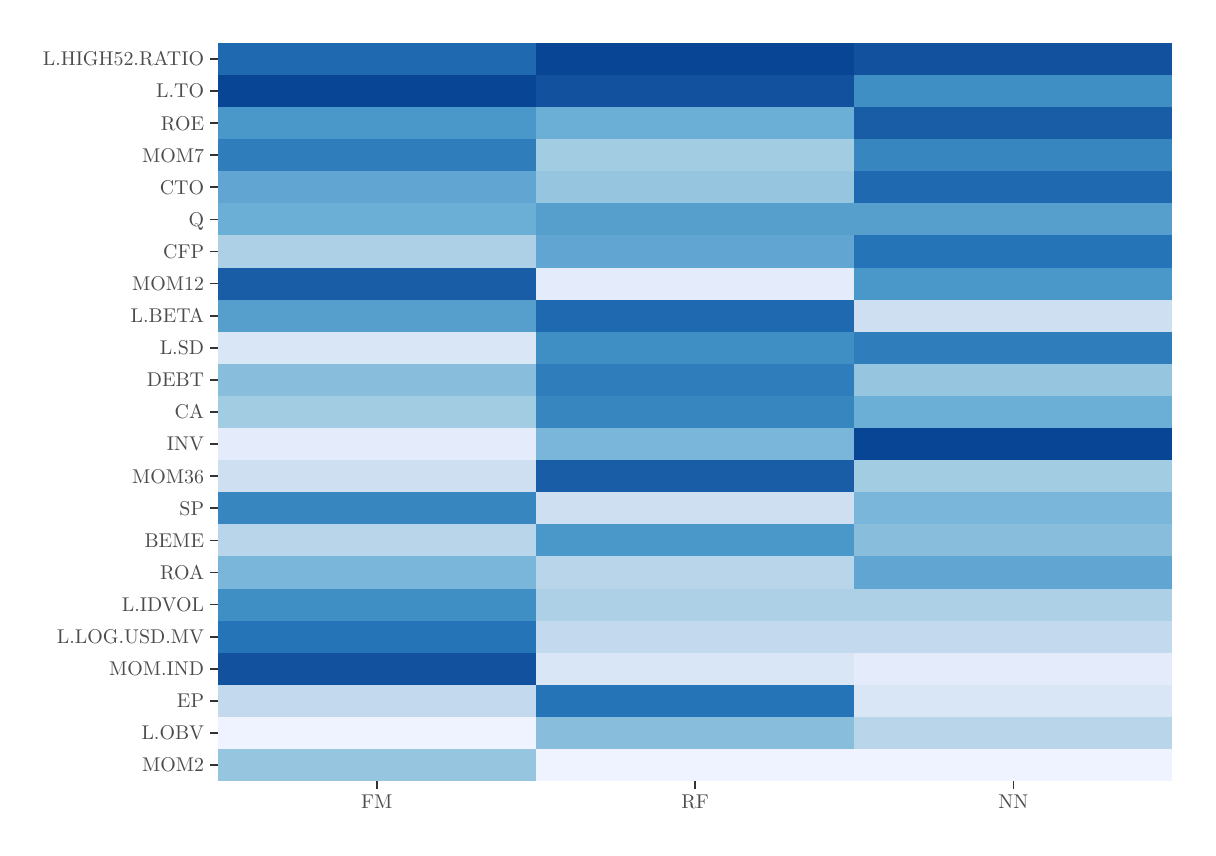
\begin{tikzpicture}[x=1pt,y=1pt]
\definecolor{fillColor}{RGB}{255,255,255}
\path[use as bounding box,fill=fillColor,fill opacity=0.00] (0,0) rectangle (419.17,289.08);
\begin{scope}
\path[clip] (  0.00,  0.00) rectangle (419.17,289.08);
\definecolor{drawColor}{RGB}{255,255,255}
\definecolor{fillColor}{RGB}{255,255,255}

\path[draw=drawColor,line width= 0.6pt,line join=round,line cap=round,fill=fillColor] (  0.00,  0.00) rectangle (419.17,289.08);
\end{scope}
\begin{scope}
\path[clip] ( 68.69, 16.81) rectangle (413.67,283.58);
\definecolor{fillColor}{gray}{0.92}

\path[fill=fillColor] ( 68.69, 16.81) rectangle (413.67,283.58);
\definecolor{drawColor}{RGB}{255,255,255}

\path[draw=drawColor,line width= 0.6pt,line join=round] ( 68.69, 22.61) --
	(413.67, 22.61);

\path[draw=drawColor,line width= 0.6pt,line join=round] ( 68.69, 34.21) --
	(413.67, 34.21);

\path[draw=drawColor,line width= 0.6pt,line join=round] ( 68.69, 45.81) --
	(413.67, 45.81);

\path[draw=drawColor,line width= 0.6pt,line join=round] ( 68.69, 57.40) --
	(413.67, 57.40);

\path[draw=drawColor,line width= 0.6pt,line join=round] ( 68.69, 69.00) --
	(413.67, 69.00);

\path[draw=drawColor,line width= 0.6pt,line join=round] ( 68.69, 80.60) --
	(413.67, 80.60);

\path[draw=drawColor,line width= 0.6pt,line join=round] ( 68.69, 92.20) --
	(413.67, 92.20);

\path[draw=drawColor,line width= 0.6pt,line join=round] ( 68.69,103.80) --
	(413.67,103.80);

\path[draw=drawColor,line width= 0.6pt,line join=round] ( 68.69,115.40) --
	(413.67,115.40);

\path[draw=drawColor,line width= 0.6pt,line join=round] ( 68.69,127.00) --
	(413.67,127.00);

\path[draw=drawColor,line width= 0.6pt,line join=round] ( 68.69,138.60) --
	(413.67,138.60);

\path[draw=drawColor,line width= 0.6pt,line join=round] ( 68.69,150.19) --
	(413.67,150.19);

\path[draw=drawColor,line width= 0.6pt,line join=round] ( 68.69,161.79) --
	(413.67,161.79);

\path[draw=drawColor,line width= 0.6pt,line join=round] ( 68.69,173.39) --
	(413.67,173.39);

\path[draw=drawColor,line width= 0.6pt,line join=round] ( 68.69,184.99) --
	(413.67,184.99);

\path[draw=drawColor,line width= 0.6pt,line join=round] ( 68.69,196.59) --
	(413.67,196.59);

\path[draw=drawColor,line width= 0.6pt,line join=round] ( 68.69,208.19) --
	(413.67,208.19);

\path[draw=drawColor,line width= 0.6pt,line join=round] ( 68.69,219.79) --
	(413.67,219.79);

\path[draw=drawColor,line width= 0.6pt,line join=round] ( 68.69,231.39) --
	(413.67,231.39);

\path[draw=drawColor,line width= 0.6pt,line join=round] ( 68.69,242.98) --
	(413.67,242.98);

\path[draw=drawColor,line width= 0.6pt,line join=round] ( 68.69,254.58) --
	(413.67,254.58);

\path[draw=drawColor,line width= 0.6pt,line join=round] ( 68.69,266.18) --
	(413.67,266.18);

\path[draw=drawColor,line width= 0.6pt,line join=round] ( 68.69,277.78) --
	(413.67,277.78);

\path[draw=drawColor,line width= 0.6pt,line join=round] (126.18, 16.81) --
	(126.18,283.58);

\path[draw=drawColor,line width= 0.6pt,line join=round] (241.18, 16.81) --
	(241.18,283.58);

\path[draw=drawColor,line width= 0.6pt,line join=round] (356.17, 16.81) --
	(356.17,283.58);
\definecolor{fillColor}{RGB}{74,151,201}

\path[fill=fillColor] (183.68, 98.00) rectangle (298.67,109.60);
\definecolor{fillColor}{RGB}{56,134,192}

\path[fill=fillColor] (183.68,144.39) rectangle (298.67,155.99);
\definecolor{fillColor}{RGB}{97,166,210}

\path[fill=fillColor] (183.68,202.39) rectangle (298.67,213.99);
\definecolor{fillColor}{RGB}{149,197,223}

\path[fill=fillColor] (183.68,225.59) rectangle (298.67,237.18);
\definecolor{fillColor}{RGB}{47,125,187}

\path[fill=fillColor] (183.68,155.99) rectangle (298.67,167.59);
\definecolor{fillColor}{RGB}{37,116,183}

\path[fill=fillColor] (183.68, 40.01) rectangle (298.67, 51.60);
\definecolor{fillColor}{RGB}{122,182,217}

\path[fill=fillColor] (183.68,132.80) rectangle (298.67,144.39);
\definecolor{fillColor}{RGB}{30,105,175}

\path[fill=fillColor] (183.68,179.19) rectangle (298.67,190.79);
\definecolor{fillColor}{RGB}{8,69,148}

\path[fill=fillColor] (183.68,271.98) rectangle (298.67,283.58);
\definecolor{fillColor}{RGB}{173,208,230}

\path[fill=fillColor] (183.68, 74.80) rectangle (298.67, 86.40);
\definecolor{fillColor}{RGB}{194,217,238}

\path[fill=fillColor] (183.68, 63.20) rectangle (298.67, 74.80);
\definecolor{fillColor}{RGB}{136,189,220}

\path[fill=fillColor] (183.68, 28.41) rectangle (298.67, 40.01);
\definecolor{fillColor}{RGB}{64,143,196}

\path[fill=fillColor] (183.68,167.59) rectangle (298.67,179.19);
\definecolor{fillColor}{RGB}{18,81,157}

\path[fill=fillColor] (183.68,260.38) rectangle (298.67,271.98);
\definecolor{fillColor}{RGB}{217,230,246}

\path[fill=fillColor] (183.68, 51.60) rectangle (298.67, 63.20);
\definecolor{fillColor}{RGB}{228,236,251}

\path[fill=fillColor] (183.68,190.79) rectangle (298.67,202.39);
\definecolor{fillColor}{RGB}{239,243,255}

\path[fill=fillColor] (183.68, 16.81) rectangle (298.67, 28.41);
\definecolor{fillColor}{RGB}{25,93,166}

\path[fill=fillColor] (183.68,121.20) rectangle (298.67,132.80);
\definecolor{fillColor}{RGB}{162,204,226}

\path[fill=fillColor] (183.68,237.18) rectangle (298.67,248.78);
\definecolor{fillColor}{RGB}{86,159,205}

\path[fill=fillColor] (183.68,213.99) rectangle (298.67,225.59);
\definecolor{fillColor}{RGB}{184,213,234}

\path[fill=fillColor] (183.68, 86.40) rectangle (298.67, 98.00);
\definecolor{fillColor}{RGB}{107,174,214}

\path[fill=fillColor] (183.68,248.78) rectangle (298.67,260.38);
\definecolor{fillColor}{RGB}{206,223,242}

\path[fill=fillColor] (183.68,109.60) rectangle (298.67,121.20);
\definecolor{fillColor}{RGB}{184,213,234}

\path[fill=fillColor] ( 68.69, 98.00) rectangle (183.68,109.60);
\definecolor{fillColor}{RGB}{162,204,226}

\path[fill=fillColor] ( 68.69,144.39) rectangle (183.68,155.99);
\definecolor{fillColor}{RGB}{173,208,230}

\path[fill=fillColor] ( 68.69,202.39) rectangle (183.68,213.99);
\definecolor{fillColor}{RGB}{97,166,210}

\path[fill=fillColor] ( 68.69,225.59) rectangle (183.68,237.18);
\definecolor{fillColor}{RGB}{136,189,220}

\path[fill=fillColor] ( 68.69,155.99) rectangle (183.68,167.59);
\definecolor{fillColor}{RGB}{194,217,238}

\path[fill=fillColor] ( 68.69, 40.01) rectangle (183.68, 51.60);
\definecolor{fillColor}{RGB}{228,236,251}

\path[fill=fillColor] ( 68.69,132.80) rectangle (183.68,144.39);
\definecolor{fillColor}{RGB}{86,159,205}

\path[fill=fillColor] ( 68.69,179.19) rectangle (183.68,190.79);
\definecolor{fillColor}{RGB}{30,105,175}

\path[fill=fillColor] ( 68.69,271.98) rectangle (183.68,283.58);
\definecolor{fillColor}{RGB}{64,143,196}

\path[fill=fillColor] ( 68.69, 74.80) rectangle (183.68, 86.40);
\definecolor{fillColor}{RGB}{37,116,183}

\path[fill=fillColor] ( 68.69, 63.20) rectangle (183.68, 74.80);
\definecolor{fillColor}{RGB}{239,243,255}

\path[fill=fillColor] ( 68.69, 28.41) rectangle (183.68, 40.01);
\definecolor{fillColor}{RGB}{217,230,246}

\path[fill=fillColor] ( 68.69,167.59) rectangle (183.68,179.19);
\definecolor{fillColor}{RGB}{8,69,148}

\path[fill=fillColor] ( 68.69,260.38) rectangle (183.68,271.98);
\definecolor{fillColor}{RGB}{18,81,157}

\path[fill=fillColor] ( 68.69, 51.60) rectangle (183.68, 63.20);
\definecolor{fillColor}{RGB}{25,93,166}

\path[fill=fillColor] ( 68.69,190.79) rectangle (183.68,202.39);
\definecolor{fillColor}{RGB}{149,197,223}

\path[fill=fillColor] ( 68.69, 16.81) rectangle (183.68, 28.41);
\definecolor{fillColor}{RGB}{206,223,242}

\path[fill=fillColor] ( 68.69,121.20) rectangle (183.68,132.80);
\definecolor{fillColor}{RGB}{47,125,187}

\path[fill=fillColor] ( 68.69,237.18) rectangle (183.68,248.78);
\definecolor{fillColor}{RGB}{107,174,214}

\path[fill=fillColor] ( 68.69,213.99) rectangle (183.68,225.59);
\definecolor{fillColor}{RGB}{122,182,217}

\path[fill=fillColor] ( 68.69, 86.40) rectangle (183.68, 98.00);
\definecolor{fillColor}{RGB}{74,151,201}

\path[fill=fillColor] ( 68.69,248.78) rectangle (183.68,260.38);
\definecolor{fillColor}{RGB}{56,134,192}

\path[fill=fillColor] ( 68.69,109.60) rectangle (183.68,121.20);
\definecolor{fillColor}{RGB}{136,189,220}

\path[fill=fillColor] (298.67, 98.00) rectangle (413.67,109.60);
\definecolor{fillColor}{RGB}{107,174,214}

\path[fill=fillColor] (298.67,144.39) rectangle (413.67,155.99);
\definecolor{fillColor}{RGB}{37,116,183}

\path[fill=fillColor] (298.67,202.39) rectangle (413.67,213.99);
\definecolor{fillColor}{RGB}{30,105,175}

\path[fill=fillColor] (298.67,225.59) rectangle (413.67,237.18);
\definecolor{fillColor}{RGB}{149,197,223}

\path[fill=fillColor] (298.67,155.99) rectangle (413.67,167.59);
\definecolor{fillColor}{RGB}{217,230,246}

\path[fill=fillColor] (298.67, 40.01) rectangle (413.67, 51.60);
\definecolor{fillColor}{RGB}{8,69,148}

\path[fill=fillColor] (298.67,132.80) rectangle (413.67,144.39);
\definecolor{fillColor}{RGB}{206,223,242}

\path[fill=fillColor] (298.67,179.19) rectangle (413.67,190.79);
\definecolor{fillColor}{RGB}{18,81,157}

\path[fill=fillColor] (298.67,271.98) rectangle (413.67,283.58);
\definecolor{fillColor}{RGB}{173,208,230}

\path[fill=fillColor] (298.67, 74.80) rectangle (413.67, 86.40);
\definecolor{fillColor}{RGB}{194,217,238}

\path[fill=fillColor] (298.67, 63.20) rectangle (413.67, 74.80);
\definecolor{fillColor}{RGB}{184,213,234}

\path[fill=fillColor] (298.67, 28.41) rectangle (413.67, 40.01);
\definecolor{fillColor}{RGB}{47,125,187}

\path[fill=fillColor] (298.67,167.59) rectangle (413.67,179.19);
\definecolor{fillColor}{RGB}{64,143,196}

\path[fill=fillColor] (298.67,260.38) rectangle (413.67,271.98);
\definecolor{fillColor}{RGB}{228,236,251}

\path[fill=fillColor] (298.67, 51.60) rectangle (413.67, 63.20);
\definecolor{fillColor}{RGB}{74,151,201}

\path[fill=fillColor] (298.67,190.79) rectangle (413.67,202.39);
\definecolor{fillColor}{RGB}{239,243,255}

\path[fill=fillColor] (298.67, 16.81) rectangle (413.67, 28.41);
\definecolor{fillColor}{RGB}{162,204,226}

\path[fill=fillColor] (298.67,121.20) rectangle (413.67,132.80);
\definecolor{fillColor}{RGB}{56,134,192}

\path[fill=fillColor] (298.67,237.18) rectangle (413.67,248.78);
\definecolor{fillColor}{RGB}{86,159,205}

\path[fill=fillColor] (298.67,213.99) rectangle (413.67,225.59);
\definecolor{fillColor}{RGB}{97,166,210}

\path[fill=fillColor] (298.67, 86.40) rectangle (413.67, 98.00);
\definecolor{fillColor}{RGB}{25,93,166}

\path[fill=fillColor] (298.67,248.78) rectangle (413.67,260.38);
\definecolor{fillColor}{RGB}{122,182,217}

\path[fill=fillColor] (298.67,109.60) rectangle (413.67,121.20);
\end{scope}
\begin{scope}
\path[clip] (  0.00,  0.00) rectangle (419.17,289.08);
\definecolor{drawColor}{gray}{0.30}

\node[text=drawColor,anchor=base east,inner sep=0pt, outer sep=0pt, scale=  0.72] at ( 63.74, 20.13) {MOM2};

\node[text=drawColor,anchor=base east,inner sep=0pt, outer sep=0pt, scale=  0.72] at ( 63.74, 31.73) {L.OBV};

\node[text=drawColor,anchor=base east,inner sep=0pt, outer sep=0pt, scale=  0.72] at ( 63.74, 43.33) {EP};

\node[text=drawColor,anchor=base east,inner sep=0pt, outer sep=0pt, scale=  0.72] at ( 63.74, 54.92) {MOM.IND};

\node[text=drawColor,anchor=base east,inner sep=0pt, outer sep=0pt, scale=  0.72] at ( 63.74, 66.52) {L.LOG.USD.MV};

\node[text=drawColor,anchor=base east,inner sep=0pt, outer sep=0pt, scale=  0.72] at ( 63.74, 78.12) {L.IDVOL};

\node[text=drawColor,anchor=base east,inner sep=0pt, outer sep=0pt, scale=  0.72] at ( 63.74, 89.72) {ROA};

\node[text=drawColor,anchor=base east,inner sep=0pt, outer sep=0pt, scale=  0.72] at ( 63.74,101.32) {BEME};

\node[text=drawColor,anchor=base east,inner sep=0pt, outer sep=0pt, scale=  0.72] at ( 63.74,112.92) {SP};

\node[text=drawColor,anchor=base east,inner sep=0pt, outer sep=0pt, scale=  0.72] at ( 63.74,124.52) {MOM36};

\node[text=drawColor,anchor=base east,inner sep=0pt, outer sep=0pt, scale=  0.72] at ( 63.74,136.12) {INV};

\node[text=drawColor,anchor=base east,inner sep=0pt, outer sep=0pt, scale=  0.72] at ( 63.74,147.71) {CA};

\node[text=drawColor,anchor=base east,inner sep=0pt, outer sep=0pt, scale=  0.72] at ( 63.74,159.31) {DEBT};

\node[text=drawColor,anchor=base east,inner sep=0pt, outer sep=0pt, scale=  0.72] at ( 63.74,170.91) {L.SD};

\node[text=drawColor,anchor=base east,inner sep=0pt, outer sep=0pt, scale=  0.72] at ( 63.74,182.51) {L.BETA};

\node[text=drawColor,anchor=base east,inner sep=0pt, outer sep=0pt, scale=  0.72] at ( 63.74,194.11) {MOM12};

\node[text=drawColor,anchor=base east,inner sep=0pt, outer sep=0pt, scale=  0.72] at ( 63.74,205.71) {CFP};

\node[text=drawColor,anchor=base east,inner sep=0pt, outer sep=0pt, scale=  0.72] at ( 63.74,217.31) {Q};

\node[text=drawColor,anchor=base east,inner sep=0pt, outer sep=0pt, scale=  0.72] at ( 63.74,228.91) {CTO};

\node[text=drawColor,anchor=base east,inner sep=0pt, outer sep=0pt, scale=  0.72] at ( 63.74,240.50) {MOM7};

\node[text=drawColor,anchor=base east,inner sep=0pt, outer sep=0pt, scale=  0.72] at ( 63.74,252.10) {ROE};

\node[text=drawColor,anchor=base east,inner sep=0pt, outer sep=0pt, scale=  0.72] at ( 63.74,263.70) {L.TO};

\node[text=drawColor,anchor=base east,inner sep=0pt, outer sep=0pt, scale=  0.72] at ( 63.74,275.30) {L.HIGH52.RATIO};
\end{scope}
\begin{scope}
\path[clip] (  0.00,  0.00) rectangle (419.17,289.08);
\definecolor{drawColor}{gray}{0.20}

\path[draw=drawColor,line width= 0.6pt,line join=round] ( 65.94, 22.61) --
	( 68.69, 22.61);

\path[draw=drawColor,line width= 0.6pt,line join=round] ( 65.94, 34.21) --
	( 68.69, 34.21);

\path[draw=drawColor,line width= 0.6pt,line join=round] ( 65.94, 45.81) --
	( 68.69, 45.81);

\path[draw=drawColor,line width= 0.6pt,line join=round] ( 65.94, 57.40) --
	( 68.69, 57.40);

\path[draw=drawColor,line width= 0.6pt,line join=round] ( 65.94, 69.00) --
	( 68.69, 69.00);

\path[draw=drawColor,line width= 0.6pt,line join=round] ( 65.94, 80.60) --
	( 68.69, 80.60);

\path[draw=drawColor,line width= 0.6pt,line join=round] ( 65.94, 92.20) --
	( 68.69, 92.20);

\path[draw=drawColor,line width= 0.6pt,line join=round] ( 65.94,103.80) --
	( 68.69,103.80);

\path[draw=drawColor,line width= 0.6pt,line join=round] ( 65.94,115.40) --
	( 68.69,115.40);

\path[draw=drawColor,line width= 0.6pt,line join=round] ( 65.94,127.00) --
	( 68.69,127.00);

\path[draw=drawColor,line width= 0.6pt,line join=round] ( 65.94,138.60) --
	( 68.69,138.60);

\path[draw=drawColor,line width= 0.6pt,line join=round] ( 65.94,150.19) --
	( 68.69,150.19);

\path[draw=drawColor,line width= 0.6pt,line join=round] ( 65.94,161.79) --
	( 68.69,161.79);

\path[draw=drawColor,line width= 0.6pt,line join=round] ( 65.94,173.39) --
	( 68.69,173.39);

\path[draw=drawColor,line width= 0.6pt,line join=round] ( 65.94,184.99) --
	( 68.69,184.99);

\path[draw=drawColor,line width= 0.6pt,line join=round] ( 65.94,196.59) --
	( 68.69,196.59);

\path[draw=drawColor,line width= 0.6pt,line join=round] ( 65.94,208.19) --
	( 68.69,208.19);

\path[draw=drawColor,line width= 0.6pt,line join=round] ( 65.94,219.79) --
	( 68.69,219.79);

\path[draw=drawColor,line width= 0.6pt,line join=round] ( 65.94,231.39) --
	( 68.69,231.39);

\path[draw=drawColor,line width= 0.6pt,line join=round] ( 65.94,242.98) --
	( 68.69,242.98);

\path[draw=drawColor,line width= 0.6pt,line join=round] ( 65.94,254.58) --
	( 68.69,254.58);

\path[draw=drawColor,line width= 0.6pt,line join=round] ( 65.94,266.18) --
	( 68.69,266.18);

\path[draw=drawColor,line width= 0.6pt,line join=round] ( 65.94,277.78) --
	( 68.69,277.78);
\end{scope}
\begin{scope}
\path[clip] (  0.00,  0.00) rectangle (419.17,289.08);
\definecolor{drawColor}{gray}{0.20}

\path[draw=drawColor,line width= 0.6pt,line join=round] (126.18, 14.06) --
	(126.18, 16.81);

\path[draw=drawColor,line width= 0.6pt,line join=round] (241.18, 14.06) --
	(241.18, 16.81);

\path[draw=drawColor,line width= 0.6pt,line join=round] (356.17, 14.06) --
	(356.17, 16.81);
\end{scope}
\begin{scope}
\path[clip] (  0.00,  0.00) rectangle (419.17,289.08);
\definecolor{drawColor}{gray}{0.30}

\node[text=drawColor,anchor=base,inner sep=0pt, outer sep=0pt, scale=  0.72] at (126.18,  6.90) {FM};

\node[text=drawColor,anchor=base,inner sep=0pt, outer sep=0pt, scale=  0.72] at (241.18,  6.90) {RF};

\node[text=drawColor,anchor=base,inner sep=0pt, outer sep=0pt, scale=  0.72] at (356.17,  6.90) {NN};
\end{scope}
\end{tikzpicture}

\label{plot:combined_VI}
\end{figure}

The most important variable among all models is the 12-month momentum. 12-month momentum shows relatively large importance in all models, which is not a big surprise given the strong performance of the momentum benchmark factor in Section \ref{BenchmarkFactorPerformance}. The momentum effect is also well documented in previous Nordic stock market anomaly literature  \citep[e.g.][]{grobys, leivo2011}. Another variable that shows a rather strong influence across the models is capital turnover. On the other hand, models agree on the low importance of on-balance volume and earnings-to-price ratio. Including the earnings-to-price ratio even reduces the prediction accuracy for two out of three models as can be seen from Figure \ref{plot:relative_VI}. One objective of this study was to examine whether on-balance volume would contain information about the future cross-section of stock returns. At least in the setting of this study information that on-balance volume can provide about future stock returns is limited. \par

Sections \ref{PredictionAccuracy} and \ref{PortfolioPerformance} showed evidence that models could be overshooting in their predictions. This phenomenon could also affect variable importance. Especially, this could be an important factor for the variable importance of the linear regression model with clearly negative out-of-sample $R^2$. Hypothetically if the exclusion of a characteristic would demean all the predictions of the linear model to 0, variable importance of this variable would be clearly positive. This is because then in the described case out-of-sample $R^2$ would be zero and since the out-of-sample $R^2$ of the full model is negative there would be a positive change in out-of-sample $R^2$. Nevertheless, after excluding this hypothetical variable model would become useless for an investor, since constant prediction would not provide any information about the cross-section of future stock returns. Therefore, the investor would not have any indicator for the portfolio construction from Section \ref{PortfolioPerformance}. \par

The above-described situation is only hypothetical, since even if the only variable containing information of the future returns would be excluded linear regression would not necessarily predict zeros, but rather cross-sectional averages. For example, the average excess return for Nordic stocks in the time period of this study is 0.7\%. Still, at least partially variable importance of certain variables could be driven by the fact that their removal just reduces the overshooting of the model. One option to investigate this would be to reproduce the expected return portfolios after the exclusion of a variable. This way it could be seen if including a variable brings the realized excess return of an expected return portfolio closer to its expected return. \par

\section{Conclusion}\label{Conclusion}

More trading variables.

Even though it is argued that the linear models do not require hyperparameter optimization, as the Fama MacBeth variation is chosen one variable could be treated as a hyperparameter. The implemented linear model requires input from the user for the rolling window used to calculate mean factor loadings. One option for further research could be to treat also linear model more like the other machine learning models and optimize the rolling window.

Discuss other hyperparameters as well.

Low variable because lot of yearly variables and few stocks allocated to each portfolio.

Rolling time window, because r2 in the end volatile. If there are indicators that predictors relation to excess return is time-varying shorter window could be justified.

\clearpage

\appendix
\section{Data collection}
\renewcommand{\thefigure}{A.\arabic{figure}}
\setcounter{figure}{0}
\renewcommand{\thetable}{A.\arabic{table}}
\setcounter{table}{0}

Data for this study is collected from Datastream. Raw data is collected using constitute sets introduced in Table \ref{table:constituteLists}. For each country research, Worldscope and dead constitute lists are considered. Including dead lists allows us to avoid survivorship bias. As shown by \citet{Ince2006} in order to ensure data quality, data from Datastream requires cleaning. Tables \ref{table:DynamicScreens}, \ref{table:StaticScreens} and \ref{table:GeneralKeywords} present the dynamic and static screens used in the data cleaning. \par

Dynamic screens from Table \ref{table:DynamicScreens} result deletion of observations from the dataset. If an observation is deleted due to a dynamic screen, corresponding security is not necessarily completely excluded from the dataset. Tables \ref{table:StaticScreens} and \ref{table:GeneralKeywords} show the static screen. The objective of these screens is to clean the dataset from non-common and duplicate stock affiliations. Panel A of Table \ref{table:StaticScreens} shows which values are accepted for certain attributes, whereas panel B of Table \ref{table:StaticScreens} and Table \ref{table:GeneralKeywords} introduce maleficent keywords that are searched among Datastream attributes NAME, ENAME and ECNAME. In case a requirement from panel A of Table \ref{table:StaticScreens} is not met or if a maleficent keyword is found in the name of the security, security is excluded from the dataset completely. \par

\begin{table}[H] 
\footnotesize
\caption[Constituent lists and keywords]{\textbf{Constituent lists and keywords}\\ Modified taken from \protect\citet{Ince2006} and \protect\citet{HANAUER2023106712}. The table provides the constituent lists used in data collection.}
 \label{table:constituteLists}
\centering
\begin{tabularx}{\textwidth}{X X X X}
\toprule
Denmark & Finland & Norway & Sweden \\
\midrule
FDEN 		&  FFIN		& FNOR		& FSWD\\
WSCOPEDK & WSCOPEFN & WSCOPENW& WSCOPESD\\
DEADDK 	&   DEADFN 	& DEADNW 	& DEADSD\\
& & & FAKTSWD\\
 \bottomrule
 \end{tabularx}
 \end{table} 
 
\begin{table}[H] 
\footnotesize
\caption[Dynamic screens]{\textbf{Dynamic screens}\\ Modified taken from \protect\citet{Ince2006} and \protect\citet{HANAUER2023106712}. The table provides the dynamics screens used in the data cleaning.}
 \label{table:DynamicScreens}
\centering
\begin{tabularx}{\textwidth}{l X}
\toprule
Affected attribute & Applied screen \\
\midrule
RI 		& Observations where the one-month return is larger than 990\% are removed.\\ \rule{-1ex}{3ex}
RI		& Observation is removed if return in $r_t$ or $r_{t-1}$ exceed 300\% and $(1+r_{t})(1+r_{t-1}) -1$ is less than 0.5. \\ \rule{-1ex}{3ex}
RI 		& For periods after the delisting of a security Datastream returns the last available value. Therefore, by removing all consecutive zero returns at the end of the dataset for all securities.\\
 \bottomrule
 \end{tabularx}
 \end{table} 

\begin{table}[H]
\footnotesize
\caption[Static screens]{\textbf{Static screens}\\ Modified taken from \protect\citet{Ince2006} and \protect\citet{HANAUER2023106712}. Panel A of the table provides the Datastream items that are considered for the filtering and accepted values for each country separately. Panel B of the table provides keywords that were used to delete entries from each market separately. The same logic is applied to remove both country-specific and generic keywords. A keyword is searched from Datastream attributes NAME, ENAME and ECNAME. In case at least one of these attributes contains the keyword security is deleted from the dataset. To avoid deleting proper entries, security is only deleted if the keyword occurs at the beginning of the name, at the end of the name or as a separate word in the name.}
\label{table:StaticScreens}
\begin{tabularx}{\textwidth}{X X X X l}
\toprule
\multicolumn{5}{l}{\textit{Panel A: Static screens.}} \\
\midrule
 & Denmark & Finland & Norway & Sweden\\
\midrule
MAJOR & Y & Y & Y & Y\\
TYPE & EQ & EQ & EQ & EQ\\
ISINID & P & P & P & P\\
GEOGN & DENMARK & FINLAND & NORWAY & SWEDEN\\
GEOLN & DENMARK & FINLAND & NORWAY & SWEDEN\\
PCUR & DK & FI, MK & NK & SK\\
GGSIN & DK & FI & NO &SE\\
\toprule
\multicolumn{5}{l}{\textit{Panel B: Country specific keywords.}} \\
\midrule
 & Denmark & Finland & Norway & Sweden\\
 \midrule
NAME & \multirow[m]{3}{*}{ \textbackslash \textbackslash)CSE \textbackslash \textbackslash} & \multirow[m]{3}{*}{USE} & & \multirow[m]{3}{13em}{CONVERTED INTO, USE, CONVERTED-, CONVERTED - SEE}\\
ENAME & & \\
ECNAME & &\\
\bottomrule
\end{tabularx}
\end{table}


\begin{table}[H] 
\footnotesize
\caption[Common keywords]{\textbf{Common keywords}\\ Modified taken from \protect\citet{Ince2006} and \protect\citet{HANAUER2023106712}. The table shows the general keywords that were used to delete entries from all markets. The same keyword deletion logic is applied to remove both country-specific and generic keywords. The keyword is searched from Datastream attributes NAME, ENAME and ECNAME. In case at least one of these attributes contains the keyword security is deleted from the dataset. To avoid deleting proper entries, security is only deleted if the keyword occurs at the beginning of the name, at the end of the name or as a separate word in the name.}
 \label{table:GeneralKeywords}
\centering
\begin{tabularx}{\textwidth}{l X}
\toprule
Security class 	& Keywords \\
\midrule
Duplicates 		& 1000DUPL, DULP, DUP, DUPE, DUPL, DUPLI, DUPLICATE, XSQ, XETa  \\[1ex]
Depository receipts	& ADR, GDR \\[1ex]
Preferred stock 	&  PF, ’PF’, PFD, PREF, PREFERRED, PRF\\ [1ex]
Warrants 			&  WARR, WARRANT, WARRANTS, WARRT, WTS, WTS2\\[1ex]
Debt 			& \%, DB, DCB, DEB, DEBENTURE, DEBENTURES, DEBT\\[1ex]
Unit trusts 		& .IT, .ITb, TST, INVESTMENTTRUST, RLSTIT, TRUST, TRUSTUNIT, TRUSTUNITS, TST, TSTUNIT, TST UNITS, UNIT, UNITTRUST, UNITS, UNT, UNTTST, UT\\[1ex]
ETFs 			& AMUNDI, ETF, INAV, ISHARES, JUNGE, LYXOR, X-TR\\[1ex]
Expired securities 	& EXPD, EXPIRED, EXPIRY, EXPY\\[1ex]
Miscellaneous 		& ADS, BOND, CAP.SHS, CONV, DEFER, DEP, DEPY, ELKS, FD, FUND, GW.FD, HI.YIELD, HIGHINCOME, IDX, INC.								\&GROWTH, INC.\&GW, INDEX, LP, MITS, MITT, MPS, NIKKEI, OPCVM, ORTF, PERQS, 												PFC, PFCL, PINES, PRTF, PTNS, PTSHP, QUIBS, QUIDS, RATE, RCPTS, REALEST, RECEIPTS, REIT, RESPT, 								RETUR, RIGHTS, RST, RTN.INC, RTS, SBVTG, SCORE, SPDR, STRYPES, TOPRS, UTS, VCT, VTG.SAS, 									XXXXX, YIELD, YLD, PF.SHS.\\
 \bottomrule
 \end{tabularx}
 \end{table} 

\clearpage

\section{Benchmark factor properties} \label{BenchmarkFactorProperties}
\renewcommand{\thefigure}{B.\arabic{figure}}
\setcounter{figure}{0}
\renewcommand{\thetable}{B.\arabic{table}}
\setcounter{table}{0}

Supplementary materials for the benchmark factors. 

\begin{table}[H]
\footnotesize
\caption[Benchmark factor correlation matrix]{\textbf{Benchmark factor correlation matrix \textnormal{- Own source}}\\ Table shows the correlations among the benchmark factors. RMRF is the average value return of the pooled Nordic market. Portfolio returns are calculated based on 2 × 3 sorts on size and one other factor. HML is the difference in the average of the value-weighted return of two high value portfolios and the average of the value-weighted return of two low value portfolios. RMW, CMA and MOM are calculated in a similar manner, but portfolio sorts are done based on investment, profitability and momentum factors. SMB is the average of the value-weighted returns of the 12 portfolios of small stocks minus the average of the value-weighted returns of the 12 portfolios of big stocks. Returns are calculated in US dollars.}
\label{table:FFfactorsCorrelations}
\centering
\newcolumntype{Y}{>{\raggedleft\arraybackslash}X}
\begin{tabularx}{\textwidth}{@{\extracolsep{4pt}} X Y Y Y Y Y Y} 
\toprule
& HML & RMW & CMA & MOM & SMB & RMRF \\
\midrule
HML & 1 & -0.5707 & 0.5542 & 0.1122 & 0.2998 & -0.2740 \\
RMW & -0.5707 & 1 & -0.5899 & 0.0857 & -0.2568 & 0.0639 \\
CMA & 0.5542 & -0.5899 & 1 & -0.0703 & 0.1777 & -0.2078 \\
MOM & 0.1122 & 0.0857 & -0.0703 & 1 & 0.1544 & -0.2040 \\
SMB & 0.2998 & -0.2568 & 0.1777 & 0.1544 & 1 & -0.2695 \\
RMRF & -0.2740 & 0.0639 & -0.2078 & -0.2040 & -0.2695 & 1 \\
\bottomrule
\end{tabularx}
\end{table}

\begin{figure}[H]
\centering
\caption[Factor autocorrelation]{\textbf{Factor autocorrelation \textnormal{- Own source}}\\ Figure plots the the benchmark factors autocorrelations. RMRF is the average value return of the pooled Nordic market. Portfolio returns are calculated based on 2 × 3 sorts on size and one other factor. HML is the difference in the average value-weighted return of two high value portfolios and the average value-weighted return of two low value portfolios. RMW, CMA and MOM are calculated in a similar manner, but portfolio sorts are done based on investment, profitability and momentum factors. SMB is the average of the value-weighted returns of the 12 portfolios of small stocks minus the average of the value-weighted returns of the 12 portfolios of big stocks. Returns are calculated in US dollars.}
% Created by tikzDevice version 0.12.6 on 2024-01-01 11:40:19
% !TEX encoding = UTF-8 Unicode
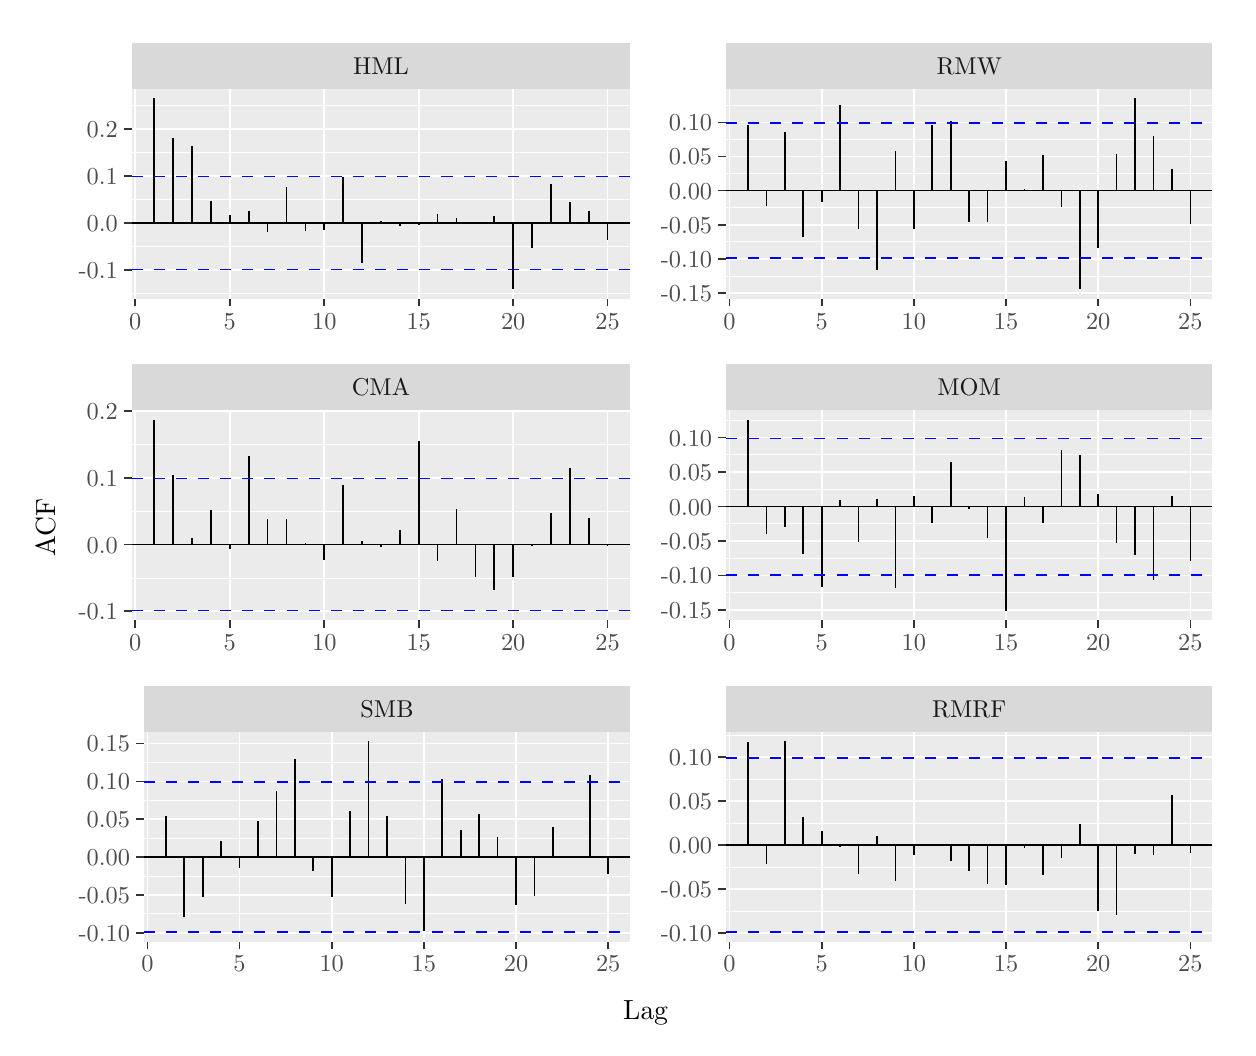
\begin{tikzpicture}[x=1pt,y=1pt]
\definecolor{fillColor}{RGB}{255,255,255}
\path[use as bounding box,fill=fillColor,fill opacity=0.00] (0,0) rectangle (433.62,361.35);
\begin{scope}
\path[clip] ( 12.91,245.20) rectangle (223.26,361.35);
\definecolor{drawColor}{RGB}{255,255,255}
\definecolor{fillColor}{RGB}{255,255,255}

\path[draw=drawColor,line width= 0.6pt,line join=round,line cap=round,fill=fillColor] ( 12.91,245.20) rectangle (223.26,361.35);
\end{scope}
\begin{scope}
\path[clip] ( 37.53,263.42) rectangle (217.76,339.28);
\definecolor{fillColor}{gray}{0.92}

\path[fill=fillColor] ( 37.53,263.42) rectangle (217.76,339.28);
\definecolor{drawColor}{RGB}{255,255,255}

\path[draw=drawColor,line width= 0.3pt,line join=round] ( 37.53,265.25) --
	(217.76,265.25);

\path[draw=drawColor,line width= 0.3pt,line join=round] ( 37.53,282.24) --
	(217.76,282.24);

\path[draw=drawColor,line width= 0.3pt,line join=round] ( 37.53,299.22) --
	(217.76,299.22);

\path[draw=drawColor,line width= 0.3pt,line join=round] ( 37.53,316.21) --
	(217.76,316.21);

\path[draw=drawColor,line width= 0.3pt,line join=round] ( 37.53,333.19) --
	(217.76,333.19);

\path[draw=drawColor,line width= 0.6pt,line join=round] ( 37.53,273.74) --
	(217.76,273.74);

\path[draw=drawColor,line width= 0.6pt,line join=round] ( 37.53,290.73) --
	(217.76,290.73);

\path[draw=drawColor,line width= 0.6pt,line join=round] ( 37.53,307.72) --
	(217.76,307.72);

\path[draw=drawColor,line width= 0.6pt,line join=round] ( 37.53,324.70) --
	(217.76,324.70);

\path[draw=drawColor,line width= 0.6pt,line join=round] ( 38.90,263.42) --
	( 38.90,339.28);

\path[draw=drawColor,line width= 0.6pt,line join=round] ( 73.03,263.42) --
	( 73.03,339.28);

\path[draw=drawColor,line width= 0.6pt,line join=round] (107.17,263.42) --
	(107.17,339.28);

\path[draw=drawColor,line width= 0.6pt,line join=round] (141.30,263.42) --
	(141.30,339.28);

\path[draw=drawColor,line width= 0.6pt,line join=round] (175.44,263.42) --
	(175.44,339.28);

\path[draw=drawColor,line width= 0.6pt,line join=round] (209.57,263.42) --
	(209.57,339.28);
\definecolor{drawColor}{RGB}{0,0,0}

\path[draw=drawColor,line width= 0.6pt,line join=round] ( 37.53,290.73) -- (217.76,290.73);

\path[draw=drawColor,line width= 0.6pt,line join=round] ( 45.73,290.73) -- ( 45.73,335.83);

\path[draw=drawColor,line width= 0.6pt,line join=round] ( 52.55,290.73) -- ( 52.55,321.43);

\path[draw=drawColor,line width= 0.6pt,line join=round] ( 59.38,290.73) -- ( 59.38,318.43);

\path[draw=drawColor,line width= 0.6pt,line join=round] ( 66.21,290.73) -- ( 66.21,298.76);

\path[draw=drawColor,line width= 0.6pt,line join=round] ( 73.03,290.73) -- ( 73.03,293.54);

\path[draw=drawColor,line width= 0.6pt,line join=round] ( 79.86,290.73) -- ( 79.86,294.99);

\path[draw=drawColor,line width= 0.6pt,line join=round] ( 86.69,290.73) -- ( 86.69,287.68);

\path[draw=drawColor,line width= 0.6pt,line join=round] ( 93.51,290.73) -- ( 93.51,303.92);

\path[draw=drawColor,line width= 0.6pt,line join=round] (100.34,290.73) -- (100.34,287.96);

\path[draw=drawColor,line width= 0.6pt,line join=round] (107.17,290.73) -- (107.17,288.35);

\path[draw=drawColor,line width= 0.6pt,line join=round] (114.00,290.73) -- (114.00,307.38);

\path[draw=drawColor,line width= 0.6pt,line join=round] (120.82,290.73) -- (120.82,276.36);

\path[draw=drawColor,line width= 0.6pt,line join=round] (127.65,290.73) -- (127.65,291.36);

\path[draw=drawColor,line width= 0.6pt,line join=round] (134.48,290.73) -- (134.48,289.50);

\path[draw=drawColor,line width= 0.6pt,line join=round] (141.30,290.73) -- (141.30,290.08);

\path[draw=drawColor,line width= 0.6pt,line join=round] (148.13,290.73) -- (148.13,293.90);

\path[draw=drawColor,line width= 0.6pt,line join=round] (154.96,290.73) -- (154.96,292.68);

\path[draw=drawColor,line width= 0.6pt,line join=round] (161.78,290.73) -- (161.78,290.30);

\path[draw=drawColor,line width= 0.6pt,line join=round] (168.61,290.73) -- (168.61,293.33);

\path[draw=drawColor,line width= 0.6pt,line join=round] (175.44,290.73) -- (175.44,266.87);

\path[draw=drawColor,line width= 0.6pt,line join=round] (182.26,290.73) -- (182.26,281.77);

\path[draw=drawColor,line width= 0.6pt,line join=round] (189.09,290.73) -- (189.09,304.71);

\path[draw=drawColor,line width= 0.6pt,line join=round] (195.92,290.73) -- (195.92,298.23);

\path[draw=drawColor,line width= 0.6pt,line join=round] (202.75,290.73) -- (202.75,294.98);

\path[draw=drawColor,line width= 0.6pt,line join=round] (209.57,290.73) -- (209.57,284.66);
\definecolor{drawColor}{RGB}{0,0,255}

\path[draw=drawColor,line width= 0.6pt,dash pattern=on 4pt off 4pt ,line join=round] ( 37.53,273.94) -- (217.76,273.94);

\path[draw=drawColor,line width= 0.6pt,dash pattern=on 4pt off 4pt ,line join=round] ( 37.53,307.52) -- (217.76,307.52);
\end{scope}
\begin{scope}
\path[clip] ( 37.53,339.28) rectangle (217.76,355.85);
\definecolor{fillColor}{gray}{0.85}

\path[fill=fillColor] ( 37.53,339.28) rectangle (217.76,355.85);
\definecolor{drawColor}{gray}{0.10}

\node[text=drawColor,anchor=base,inner sep=0pt, outer sep=0pt, scale=  0.88] at (127.65,344.53) {HML};
\end{scope}
\begin{scope}
\path[clip] (  0.00,  0.00) rectangle (433.62,361.35);
\definecolor{drawColor}{gray}{0.20}

\path[draw=drawColor,line width= 0.6pt,line join=round] ( 38.90,260.67) --
	( 38.90,263.42);

\path[draw=drawColor,line width= 0.6pt,line join=round] ( 73.03,260.67) --
	( 73.03,263.42);

\path[draw=drawColor,line width= 0.6pt,line join=round] (107.17,260.67) --
	(107.17,263.42);

\path[draw=drawColor,line width= 0.6pt,line join=round] (141.30,260.67) --
	(141.30,263.42);

\path[draw=drawColor,line width= 0.6pt,line join=round] (175.44,260.67) --
	(175.44,263.42);

\path[draw=drawColor,line width= 0.6pt,line join=round] (209.57,260.67) --
	(209.57,263.42);
\end{scope}
\begin{scope}
\path[clip] (  0.00,  0.00) rectangle (433.62,361.35);
\definecolor{drawColor}{gray}{0.30}

\node[text=drawColor,anchor=base,inner sep=0pt, outer sep=0pt, scale=  0.88] at ( 38.90,252.41) {0};

\node[text=drawColor,anchor=base,inner sep=0pt, outer sep=0pt, scale=  0.88] at ( 73.03,252.41) {5};

\node[text=drawColor,anchor=base,inner sep=0pt, outer sep=0pt, scale=  0.88] at (107.17,252.41) {10};

\node[text=drawColor,anchor=base,inner sep=0pt, outer sep=0pt, scale=  0.88] at (141.30,252.41) {15};

\node[text=drawColor,anchor=base,inner sep=0pt, outer sep=0pt, scale=  0.88] at (175.44,252.41) {20};

\node[text=drawColor,anchor=base,inner sep=0pt, outer sep=0pt, scale=  0.88] at (209.57,252.41) {25};
\end{scope}
\begin{scope}
\path[clip] (  0.00,  0.00) rectangle (433.62,361.35);
\definecolor{drawColor}{gray}{0.30}

\node[text=drawColor,anchor=base east,inner sep=0pt, outer sep=0pt, scale=  0.88] at ( 32.58,270.71) {-0.1};

\node[text=drawColor,anchor=base east,inner sep=0pt, outer sep=0pt, scale=  0.88] at ( 32.58,287.70) {0.0};

\node[text=drawColor,anchor=base east,inner sep=0pt, outer sep=0pt, scale=  0.88] at ( 32.58,304.69) {0.1};

\node[text=drawColor,anchor=base east,inner sep=0pt, outer sep=0pt, scale=  0.88] at ( 32.58,321.67) {0.2};
\end{scope}
\begin{scope}
\path[clip] (  0.00,  0.00) rectangle (433.62,361.35);
\definecolor{drawColor}{gray}{0.20}

\path[draw=drawColor,line width= 0.6pt,line join=round] ( 34.78,273.74) --
	( 37.53,273.74);

\path[draw=drawColor,line width= 0.6pt,line join=round] ( 34.78,290.73) --
	( 37.53,290.73);

\path[draw=drawColor,line width= 0.6pt,line join=round] ( 34.78,307.72) --
	( 37.53,307.72);

\path[draw=drawColor,line width= 0.6pt,line join=round] ( 34.78,324.70) --
	( 37.53,324.70);
\end{scope}
\begin{scope}
\path[clip] (223.26,245.20) rectangle (433.62,361.35);
\definecolor{drawColor}{RGB}{255,255,255}
\definecolor{fillColor}{RGB}{255,255,255}

\path[draw=drawColor,line width= 0.6pt,line join=round,line cap=round,fill=fillColor] (223.26,245.20) rectangle (433.62,361.35);
\end{scope}
\begin{scope}
\path[clip] (252.29,263.42) rectangle (428.12,339.28);
\definecolor{fillColor}{gray}{0.92}

\path[fill=fillColor] (252.29,263.42) rectangle (428.12,339.28);
\definecolor{drawColor}{RGB}{255,255,255}

\path[draw=drawColor,line width= 0.3pt,line join=round] (252.29,271.63) --
	(428.12,271.63);

\path[draw=drawColor,line width= 0.3pt,line join=round] (252.29,283.96) --
	(428.12,283.96);

\path[draw=drawColor,line width= 0.3pt,line join=round] (252.29,296.29) --
	(428.12,296.29);

\path[draw=drawColor,line width= 0.3pt,line join=round] (252.29,308.62) --
	(428.12,308.62);

\path[draw=drawColor,line width= 0.3pt,line join=round] (252.29,320.95) --
	(428.12,320.95);

\path[draw=drawColor,line width= 0.3pt,line join=round] (252.29,333.27) --
	(428.12,333.27);

\path[draw=drawColor,line width= 0.6pt,line join=round] (252.29,265.46) --
	(428.12,265.46);

\path[draw=drawColor,line width= 0.6pt,line join=round] (252.29,277.79) --
	(428.12,277.79);

\path[draw=drawColor,line width= 0.6pt,line join=round] (252.29,290.12) --
	(428.12,290.12);

\path[draw=drawColor,line width= 0.6pt,line join=round] (252.29,302.45) --
	(428.12,302.45);

\path[draw=drawColor,line width= 0.6pt,line join=round] (252.29,314.78) --
	(428.12,314.78);

\path[draw=drawColor,line width= 0.6pt,line join=round] (252.29,327.11) --
	(428.12,327.11);

\path[draw=drawColor,line width= 0.6pt,line join=round] (253.62,263.42) --
	(253.62,339.28);

\path[draw=drawColor,line width= 0.6pt,line join=round] (286.92,263.42) --
	(286.92,339.28);

\path[draw=drawColor,line width= 0.6pt,line join=round] (320.22,263.42) --
	(320.22,339.28);

\path[draw=drawColor,line width= 0.6pt,line join=round] (353.52,263.42) --
	(353.52,339.28);

\path[draw=drawColor,line width= 0.6pt,line join=round] (386.83,263.42) --
	(386.83,339.28);

\path[draw=drawColor,line width= 0.6pt,line join=round] (420.13,263.42) --
	(420.13,339.28);
\definecolor{drawColor}{RGB}{0,0,0}

\path[draw=drawColor,line width= 0.6pt,line join=round] (252.29,302.45) -- (428.12,302.45);

\path[draw=drawColor,line width= 0.6pt,line join=round] (260.28,302.45) -- (260.28,326.14);

\path[draw=drawColor,line width= 0.6pt,line join=round] (266.94,302.45) -- (266.94,297.04);

\path[draw=drawColor,line width= 0.6pt,line join=round] (273.60,302.45) -- (273.60,323.62);

\path[draw=drawColor,line width= 0.6pt,line join=round] (280.26,302.45) -- (280.26,285.77);

\path[draw=drawColor,line width= 0.6pt,line join=round] (286.92,302.45) -- (286.92,298.49);

\path[draw=drawColor,line width= 0.6pt,line join=round] (293.58,302.45) -- (293.58,333.58);

\path[draw=drawColor,line width= 0.6pt,line join=round] (300.24,302.45) -- (300.24,288.71);

\path[draw=drawColor,line width= 0.6pt,line join=round] (306.90,302.45) -- (306.90,273.85);

\path[draw=drawColor,line width= 0.6pt,line join=round] (313.56,302.45) -- (313.56,316.96);

\path[draw=drawColor,line width= 0.6pt,line join=round] (320.22,302.45) -- (320.22,288.61);

\path[draw=drawColor,line width= 0.6pt,line join=round] (326.88,302.45) -- (326.88,326.12);

\path[draw=drawColor,line width= 0.6pt,line join=round] (333.54,302.45) -- (333.54,327.62);

\path[draw=drawColor,line width= 0.6pt,line join=round] (340.20,302.45) -- (340.20,291.09);

\path[draw=drawColor,line width= 0.6pt,line join=round] (346.86,302.45) -- (346.86,290.95);

\path[draw=drawColor,line width= 0.6pt,line join=round] (353.52,302.45) -- (353.52,313.17);

\path[draw=drawColor,line width= 0.6pt,line join=round] (360.18,302.45) -- (360.18,303.11);

\path[draw=drawColor,line width= 0.6pt,line join=round] (366.85,302.45) -- (366.85,315.38);

\path[draw=drawColor,line width= 0.6pt,line join=round] (373.51,302.45) -- (373.51,296.45);

\path[draw=drawColor,line width= 0.6pt,line join=round] (380.17,302.45) -- (380.17,266.87);

\path[draw=drawColor,line width= 0.6pt,line join=round] (386.83,302.45) -- (386.83,281.57);

\path[draw=drawColor,line width= 0.6pt,line join=round] (393.49,302.45) -- (393.49,315.55);

\path[draw=drawColor,line width= 0.6pt,line join=round] (400.15,302.45) -- (400.15,335.83);

\path[draw=drawColor,line width= 0.6pt,line join=round] (406.81,302.45) -- (406.81,322.22);

\path[draw=drawColor,line width= 0.6pt,line join=round] (413.47,302.45) -- (413.47,310.33);

\path[draw=drawColor,line width= 0.6pt,line join=round] (420.13,302.45) -- (420.13,290.32);
\definecolor{drawColor}{RGB}{0,0,255}

\path[draw=drawColor,line width= 0.6pt,dash pattern=on 4pt off 4pt ,line join=round] (252.29,278.07) -- (428.12,278.07);

\path[draw=drawColor,line width= 0.6pt,dash pattern=on 4pt off 4pt ,line join=round] (252.29,326.83) -- (428.12,326.83);
\end{scope}
\begin{scope}
\path[clip] (252.29,339.28) rectangle (428.12,355.85);
\definecolor{fillColor}{gray}{0.85}

\path[fill=fillColor] (252.29,339.28) rectangle (428.12,355.85);
\definecolor{drawColor}{gray}{0.10}

\node[text=drawColor,anchor=base,inner sep=0pt, outer sep=0pt, scale=  0.88] at (340.20,344.53) {RMW};
\end{scope}
\begin{scope}
\path[clip] (  0.00,  0.00) rectangle (433.62,361.35);
\definecolor{drawColor}{gray}{0.20}

\path[draw=drawColor,line width= 0.6pt,line join=round] (253.62,260.67) --
	(253.62,263.42);

\path[draw=drawColor,line width= 0.6pt,line join=round] (286.92,260.67) --
	(286.92,263.42);

\path[draw=drawColor,line width= 0.6pt,line join=round] (320.22,260.67) --
	(320.22,263.42);

\path[draw=drawColor,line width= 0.6pt,line join=round] (353.52,260.67) --
	(353.52,263.42);

\path[draw=drawColor,line width= 0.6pt,line join=round] (386.83,260.67) --
	(386.83,263.42);

\path[draw=drawColor,line width= 0.6pt,line join=round] (420.13,260.67) --
	(420.13,263.42);
\end{scope}
\begin{scope}
\path[clip] (  0.00,  0.00) rectangle (433.62,361.35);
\definecolor{drawColor}{gray}{0.30}

\node[text=drawColor,anchor=base,inner sep=0pt, outer sep=0pt, scale=  0.88] at (253.62,252.41) {0};

\node[text=drawColor,anchor=base,inner sep=0pt, outer sep=0pt, scale=  0.88] at (286.92,252.41) {5};

\node[text=drawColor,anchor=base,inner sep=0pt, outer sep=0pt, scale=  0.88] at (320.22,252.41) {10};

\node[text=drawColor,anchor=base,inner sep=0pt, outer sep=0pt, scale=  0.88] at (353.52,252.41) {15};

\node[text=drawColor,anchor=base,inner sep=0pt, outer sep=0pt, scale=  0.88] at (386.83,252.41) {20};

\node[text=drawColor,anchor=base,inner sep=0pt, outer sep=0pt, scale=  0.88] at (420.13,252.41) {25};
\end{scope}
\begin{scope}
\path[clip] (  0.00,  0.00) rectangle (433.62,361.35);
\definecolor{drawColor}{gray}{0.30}

\node[text=drawColor,anchor=base east,inner sep=0pt, outer sep=0pt, scale=  0.88] at (247.34,262.43) {-0.15};

\node[text=drawColor,anchor=base east,inner sep=0pt, outer sep=0pt, scale=  0.88] at (247.34,274.76) {-0.10};

\node[text=drawColor,anchor=base east,inner sep=0pt, outer sep=0pt, scale=  0.88] at (247.34,287.09) {-0.05};

\node[text=drawColor,anchor=base east,inner sep=0pt, outer sep=0pt, scale=  0.88] at (247.34,299.42) {0.00};

\node[text=drawColor,anchor=base east,inner sep=0pt, outer sep=0pt, scale=  0.88] at (247.34,311.75) {0.05};

\node[text=drawColor,anchor=base east,inner sep=0pt, outer sep=0pt, scale=  0.88] at (247.34,324.08) {0.10};
\end{scope}
\begin{scope}
\path[clip] (  0.00,  0.00) rectangle (433.62,361.35);
\definecolor{drawColor}{gray}{0.20}

\path[draw=drawColor,line width= 0.6pt,line join=round] (249.54,265.46) --
	(252.29,265.46);

\path[draw=drawColor,line width= 0.6pt,line join=round] (249.54,277.79) --
	(252.29,277.79);

\path[draw=drawColor,line width= 0.6pt,line join=round] (249.54,290.12) --
	(252.29,290.12);

\path[draw=drawColor,line width= 0.6pt,line join=round] (249.54,302.45) --
	(252.29,302.45);

\path[draw=drawColor,line width= 0.6pt,line join=round] (249.54,314.78) --
	(252.29,314.78);

\path[draw=drawColor,line width= 0.6pt,line join=round] (249.54,327.11) --
	(252.29,327.11);
\end{scope}
\begin{scope}
\path[clip] ( 12.91,129.06) rectangle (223.26,245.20);
\definecolor{drawColor}{RGB}{255,255,255}
\definecolor{fillColor}{RGB}{255,255,255}

\path[draw=drawColor,line width= 0.6pt,line join=round,line cap=round,fill=fillColor] ( 12.91,129.06) rectangle (223.26,245.20);
\end{scope}
\begin{scope}
\path[clip] ( 37.53,147.28) rectangle (217.76,223.13);
\definecolor{fillColor}{gray}{0.92}

\path[fill=fillColor] ( 37.53,147.28) rectangle (217.76,223.13);
\definecolor{drawColor}{RGB}{255,255,255}

\path[draw=drawColor,line width= 0.3pt,line join=round] ( 37.53,162.50) --
	(217.76,162.50);

\path[draw=drawColor,line width= 0.3pt,line join=round] ( 37.53,186.61) --
	(217.76,186.61);

\path[draw=drawColor,line width= 0.3pt,line join=round] ( 37.53,210.71) --
	(217.76,210.71);

\path[draw=drawColor,line width= 0.6pt,line join=round] ( 37.53,150.45) --
	(217.76,150.45);

\path[draw=drawColor,line width= 0.6pt,line join=round] ( 37.53,174.55) --
	(217.76,174.55);

\path[draw=drawColor,line width= 0.6pt,line join=round] ( 37.53,198.66) --
	(217.76,198.66);

\path[draw=drawColor,line width= 0.6pt,line join=round] ( 37.53,222.76) --
	(217.76,222.76);

\path[draw=drawColor,line width= 0.6pt,line join=round] ( 38.90,147.28) --
	( 38.90,223.13);

\path[draw=drawColor,line width= 0.6pt,line join=round] ( 73.03,147.28) --
	( 73.03,223.13);

\path[draw=drawColor,line width= 0.6pt,line join=round] (107.17,147.28) --
	(107.17,223.13);

\path[draw=drawColor,line width= 0.6pt,line join=round] (141.30,147.28) --
	(141.30,223.13);

\path[draw=drawColor,line width= 0.6pt,line join=round] (175.44,147.28) --
	(175.44,223.13);

\path[draw=drawColor,line width= 0.6pt,line join=round] (209.57,147.28) --
	(209.57,223.13);
\definecolor{drawColor}{RGB}{0,0,0}

\path[draw=drawColor,line width= 0.6pt,line join=round] ( 37.53,174.55) -- (217.76,174.55);

\path[draw=drawColor,line width= 0.6pt,line join=round] ( 45.73,174.55) -- ( 45.73,219.68);

\path[draw=drawColor,line width= 0.6pt,line join=round] ( 52.55,174.55) -- ( 52.55,199.74);

\path[draw=drawColor,line width= 0.6pt,line join=round] ( 59.38,174.55) -- ( 59.38,177.11);

\path[draw=drawColor,line width= 0.6pt,line join=round] ( 66.21,174.55) -- ( 66.21,187.23);

\path[draw=drawColor,line width= 0.6pt,line join=round] ( 73.03,174.55) -- ( 73.03,172.99);

\path[draw=drawColor,line width= 0.6pt,line join=round] ( 79.86,174.55) -- ( 79.86,206.57);

\path[draw=drawColor,line width= 0.6pt,line join=round] ( 86.69,174.55) -- ( 86.69,183.69);

\path[draw=drawColor,line width= 0.6pt,line join=round] ( 93.51,174.55) -- ( 93.51,183.65);

\path[draw=drawColor,line width= 0.6pt,line join=round] (100.34,174.55) -- (100.34,175.11);

\path[draw=drawColor,line width= 0.6pt,line join=round] (107.17,174.55) -- (107.17,169.04);

\path[draw=drawColor,line width= 0.6pt,line join=round] (114.00,174.55) -- (114.00,196.19);

\path[draw=drawColor,line width= 0.6pt,line join=round] (120.82,174.55) -- (120.82,175.89);

\path[draw=drawColor,line width= 0.6pt,line join=round] (127.65,174.55) -- (127.65,173.64);

\path[draw=drawColor,line width= 0.6pt,line join=round] (134.48,174.55) -- (134.48,180.00);

\path[draw=drawColor,line width= 0.6pt,line join=round] (141.30,174.55) -- (141.30,211.82);

\path[draw=drawColor,line width= 0.6pt,line join=round] (148.13,174.55) -- (148.13,168.51);

\path[draw=drawColor,line width= 0.6pt,line join=round] (154.96,174.55) -- (154.96,187.37);

\path[draw=drawColor,line width= 0.6pt,line join=round] (161.78,174.55) -- (161.78,162.72);

\path[draw=drawColor,line width= 0.6pt,line join=round] (168.61,174.55) -- (168.61,158.07);

\path[draw=drawColor,line width= 0.6pt,line join=round] (175.44,174.55) -- (175.44,162.86);

\path[draw=drawColor,line width= 0.6pt,line join=round] (182.26,174.55) -- (182.26,174.26);

\path[draw=drawColor,line width= 0.6pt,line join=round] (189.09,174.55) -- (189.09,185.90);

\path[draw=drawColor,line width= 0.6pt,line join=round] (195.92,174.55) -- (195.92,202.35);

\path[draw=drawColor,line width= 0.6pt,line join=round] (202.75,174.55) -- (202.75,184.04);

\path[draw=drawColor,line width= 0.6pt,line join=round] (209.57,174.55) -- (209.57,174.16);
\definecolor{drawColor}{RGB}{0,0,255}

\path[draw=drawColor,line width= 0.6pt,dash pattern=on 4pt off 4pt ,line join=round] ( 37.53,150.73) -- (217.76,150.73);

\path[draw=drawColor,line width= 0.6pt,dash pattern=on 4pt off 4pt ,line join=round] ( 37.53,198.38) -- (217.76,198.38);
\end{scope}
\begin{scope}
\path[clip] ( 37.53,223.13) rectangle (217.76,239.70);
\definecolor{fillColor}{gray}{0.85}

\path[fill=fillColor] ( 37.53,223.13) rectangle (217.76,239.70);
\definecolor{drawColor}{gray}{0.10}

\node[text=drawColor,anchor=base,inner sep=0pt, outer sep=0pt, scale=  0.88] at (127.65,228.39) {CMA};
\end{scope}
\begin{scope}
\path[clip] (  0.00,  0.00) rectangle (433.62,361.35);
\definecolor{drawColor}{gray}{0.20}

\path[draw=drawColor,line width= 0.6pt,line join=round] ( 38.90,144.53) --
	( 38.90,147.28);

\path[draw=drawColor,line width= 0.6pt,line join=round] ( 73.03,144.53) --
	( 73.03,147.28);

\path[draw=drawColor,line width= 0.6pt,line join=round] (107.17,144.53) --
	(107.17,147.28);

\path[draw=drawColor,line width= 0.6pt,line join=round] (141.30,144.53) --
	(141.30,147.28);

\path[draw=drawColor,line width= 0.6pt,line join=round] (175.44,144.53) --
	(175.44,147.28);

\path[draw=drawColor,line width= 0.6pt,line join=round] (209.57,144.53) --
	(209.57,147.28);
\end{scope}
\begin{scope}
\path[clip] (  0.00,  0.00) rectangle (433.62,361.35);
\definecolor{drawColor}{gray}{0.30}

\node[text=drawColor,anchor=base,inner sep=0pt, outer sep=0pt, scale=  0.88] at ( 38.90,136.27) {0};

\node[text=drawColor,anchor=base,inner sep=0pt, outer sep=0pt, scale=  0.88] at ( 73.03,136.27) {5};

\node[text=drawColor,anchor=base,inner sep=0pt, outer sep=0pt, scale=  0.88] at (107.17,136.27) {10};

\node[text=drawColor,anchor=base,inner sep=0pt, outer sep=0pt, scale=  0.88] at (141.30,136.27) {15};

\node[text=drawColor,anchor=base,inner sep=0pt, outer sep=0pt, scale=  0.88] at (175.44,136.27) {20};

\node[text=drawColor,anchor=base,inner sep=0pt, outer sep=0pt, scale=  0.88] at (209.57,136.27) {25};
\end{scope}
\begin{scope}
\path[clip] (  0.00,  0.00) rectangle (433.62,361.35);
\definecolor{drawColor}{gray}{0.30}

\node[text=drawColor,anchor=base east,inner sep=0pt, outer sep=0pt, scale=  0.88] at ( 32.58,147.42) {-0.1};

\node[text=drawColor,anchor=base east,inner sep=0pt, outer sep=0pt, scale=  0.88] at ( 32.58,171.52) {0.0};

\node[text=drawColor,anchor=base east,inner sep=0pt, outer sep=0pt, scale=  0.88] at ( 32.58,195.63) {0.1};

\node[text=drawColor,anchor=base east,inner sep=0pt, outer sep=0pt, scale=  0.88] at ( 32.58,219.73) {0.2};
\end{scope}
\begin{scope}
\path[clip] (  0.00,  0.00) rectangle (433.62,361.35);
\definecolor{drawColor}{gray}{0.20}

\path[draw=drawColor,line width= 0.6pt,line join=round] ( 34.78,150.45) --
	( 37.53,150.45);

\path[draw=drawColor,line width= 0.6pt,line join=round] ( 34.78,174.55) --
	( 37.53,174.55);

\path[draw=drawColor,line width= 0.6pt,line join=round] ( 34.78,198.66) --
	( 37.53,198.66);

\path[draw=drawColor,line width= 0.6pt,line join=round] ( 34.78,222.76) --
	( 37.53,222.76);
\end{scope}
\begin{scope}
\path[clip] (223.26,129.06) rectangle (433.62,245.20);
\definecolor{drawColor}{RGB}{255,255,255}
\definecolor{fillColor}{RGB}{255,255,255}

\path[draw=drawColor,line width= 0.6pt,line join=round,line cap=round,fill=fillColor] (223.26,129.06) rectangle (433.62,245.20);
\end{scope}
\begin{scope}
\path[clip] (252.29,147.28) rectangle (428.12,223.13);
\definecolor{fillColor}{gray}{0.92}

\path[fill=fillColor] (252.29,147.28) rectangle (428.12,223.13);
\definecolor{drawColor}{RGB}{255,255,255}

\path[draw=drawColor,line width= 0.3pt,line join=round] (252.29,157.13) --
	(428.12,157.13);

\path[draw=drawColor,line width= 0.3pt,line join=round] (252.29,169.59) --
	(428.12,169.59);

\path[draw=drawColor,line width= 0.3pt,line join=round] (252.29,182.05) --
	(428.12,182.05);

\path[draw=drawColor,line width= 0.3pt,line join=round] (252.29,194.51) --
	(428.12,194.51);

\path[draw=drawColor,line width= 0.3pt,line join=round] (252.29,206.97) --
	(428.12,206.97);

\path[draw=drawColor,line width= 0.3pt,line join=round] (252.29,219.44) --
	(428.12,219.44);

\path[draw=drawColor,line width= 0.6pt,line join=round] (252.29,150.90) --
	(428.12,150.90);

\path[draw=drawColor,line width= 0.6pt,line join=round] (252.29,163.36) --
	(428.12,163.36);

\path[draw=drawColor,line width= 0.6pt,line join=round] (252.29,175.82) --
	(428.12,175.82);

\path[draw=drawColor,line width= 0.6pt,line join=round] (252.29,188.28) --
	(428.12,188.28);

\path[draw=drawColor,line width= 0.6pt,line join=round] (252.29,200.74) --
	(428.12,200.74);

\path[draw=drawColor,line width= 0.6pt,line join=round] (252.29,213.20) --
	(428.12,213.20);

\path[draw=drawColor,line width= 0.6pt,line join=round] (253.62,147.28) --
	(253.62,223.13);

\path[draw=drawColor,line width= 0.6pt,line join=round] (286.92,147.28) --
	(286.92,223.13);

\path[draw=drawColor,line width= 0.6pt,line join=round] (320.22,147.28) --
	(320.22,223.13);

\path[draw=drawColor,line width= 0.6pt,line join=round] (353.52,147.28) --
	(353.52,223.13);

\path[draw=drawColor,line width= 0.6pt,line join=round] (386.83,147.28) --
	(386.83,223.13);

\path[draw=drawColor,line width= 0.6pt,line join=round] (420.13,147.28) --
	(420.13,223.13);
\definecolor{drawColor}{RGB}{0,0,0}

\path[draw=drawColor,line width= 0.6pt,line join=round] (252.29,188.28) -- (428.12,188.28);

\path[draw=drawColor,line width= 0.6pt,line join=round] (260.28,188.28) -- (260.28,219.68);

\path[draw=drawColor,line width= 0.6pt,line join=round] (266.94,188.28) -- (266.94,178.54);

\path[draw=drawColor,line width= 0.6pt,line join=round] (273.60,188.28) -- (273.60,180.92);

\path[draw=drawColor,line width= 0.6pt,line join=round] (280.26,188.28) -- (280.26,171.00);

\path[draw=drawColor,line width= 0.6pt,line join=round] (286.92,188.28) -- (286.92,159.13);

\path[draw=drawColor,line width= 0.6pt,line join=round] (293.58,188.28) -- (293.58,190.62);

\path[draw=drawColor,line width= 0.6pt,line join=round] (300.24,188.28) -- (300.24,175.67);

\path[draw=drawColor,line width= 0.6pt,line join=round] (306.90,188.28) -- (306.90,191.03);

\path[draw=drawColor,line width= 0.6pt,line join=round] (313.56,188.28) -- (313.56,158.99);

\path[draw=drawColor,line width= 0.6pt,line join=round] (320.22,188.28) -- (320.22,192.18);

\path[draw=drawColor,line width= 0.6pt,line join=round] (326.88,188.28) -- (326.88,182.37);

\path[draw=drawColor,line width= 0.6pt,line join=round] (333.54,188.28) -- (333.54,204.54);

\path[draw=drawColor,line width= 0.6pt,line join=round] (340.20,188.28) -- (340.20,187.60);

\path[draw=drawColor,line width= 0.6pt,line join=round] (346.86,188.28) -- (346.86,176.89);

\path[draw=drawColor,line width= 0.6pt,line join=round] (353.52,188.28) -- (353.52,150.73);

\path[draw=drawColor,line width= 0.6pt,line join=round] (360.18,188.28) -- (360.18,191.85);

\path[draw=drawColor,line width= 0.6pt,line join=round] (366.85,188.28) -- (366.85,182.21);

\path[draw=drawColor,line width= 0.6pt,line join=round] (373.51,188.28) -- (373.51,208.71);

\path[draw=drawColor,line width= 0.6pt,line join=round] (380.17,188.28) -- (380.17,206.92);

\path[draw=drawColor,line width= 0.6pt,line join=round] (386.83,188.28) -- (386.83,193.01);

\path[draw=drawColor,line width= 0.6pt,line join=round] (393.49,188.28) -- (393.49,175.08);

\path[draw=drawColor,line width= 0.6pt,line join=round] (400.15,188.28) -- (400.15,170.64);

\path[draw=drawColor,line width= 0.6pt,line join=round] (406.81,188.28) -- (406.81,161.77);

\path[draw=drawColor,line width= 0.6pt,line join=round] (413.47,188.28) -- (413.47,192.00);

\path[draw=drawColor,line width= 0.6pt,line join=round] (420.13,188.28) -- (420.13,168.81);
\definecolor{drawColor}{RGB}{0,0,255}

\path[draw=drawColor,line width= 0.6pt,dash pattern=on 4pt off 4pt ,line join=round] (252.29,163.64) -- (428.12,163.64);

\path[draw=drawColor,line width= 0.6pt,dash pattern=on 4pt off 4pt ,line join=round] (252.29,212.92) -- (428.12,212.92);
\end{scope}
\begin{scope}
\path[clip] (252.29,223.13) rectangle (428.12,239.70);
\definecolor{fillColor}{gray}{0.85}

\path[fill=fillColor] (252.29,223.13) rectangle (428.12,239.70);
\definecolor{drawColor}{gray}{0.10}

\node[text=drawColor,anchor=base,inner sep=0pt, outer sep=0pt, scale=  0.88] at (340.20,228.39) {MOM};
\end{scope}
\begin{scope}
\path[clip] (  0.00,  0.00) rectangle (433.62,361.35);
\definecolor{drawColor}{gray}{0.20}

\path[draw=drawColor,line width= 0.6pt,line join=round] (253.62,144.53) --
	(253.62,147.28);

\path[draw=drawColor,line width= 0.6pt,line join=round] (286.92,144.53) --
	(286.92,147.28);

\path[draw=drawColor,line width= 0.6pt,line join=round] (320.22,144.53) --
	(320.22,147.28);

\path[draw=drawColor,line width= 0.6pt,line join=round] (353.52,144.53) --
	(353.52,147.28);

\path[draw=drawColor,line width= 0.6pt,line join=round] (386.83,144.53) --
	(386.83,147.28);

\path[draw=drawColor,line width= 0.6pt,line join=round] (420.13,144.53) --
	(420.13,147.28);
\end{scope}
\begin{scope}
\path[clip] (  0.00,  0.00) rectangle (433.62,361.35);
\definecolor{drawColor}{gray}{0.30}

\node[text=drawColor,anchor=base,inner sep=0pt, outer sep=0pt, scale=  0.88] at (253.62,136.27) {0};

\node[text=drawColor,anchor=base,inner sep=0pt, outer sep=0pt, scale=  0.88] at (286.92,136.27) {5};

\node[text=drawColor,anchor=base,inner sep=0pt, outer sep=0pt, scale=  0.88] at (320.22,136.27) {10};

\node[text=drawColor,anchor=base,inner sep=0pt, outer sep=0pt, scale=  0.88] at (353.52,136.27) {15};

\node[text=drawColor,anchor=base,inner sep=0pt, outer sep=0pt, scale=  0.88] at (386.83,136.27) {20};

\node[text=drawColor,anchor=base,inner sep=0pt, outer sep=0pt, scale=  0.88] at (420.13,136.27) {25};
\end{scope}
\begin{scope}
\path[clip] (  0.00,  0.00) rectangle (433.62,361.35);
\definecolor{drawColor}{gray}{0.30}

\node[text=drawColor,anchor=base east,inner sep=0pt, outer sep=0pt, scale=  0.88] at (247.34,147.86) {-0.15};

\node[text=drawColor,anchor=base east,inner sep=0pt, outer sep=0pt, scale=  0.88] at (247.34,160.33) {-0.10};

\node[text=drawColor,anchor=base east,inner sep=0pt, outer sep=0pt, scale=  0.88] at (247.34,172.79) {-0.05};

\node[text=drawColor,anchor=base east,inner sep=0pt, outer sep=0pt, scale=  0.88] at (247.34,185.25) {0.00};

\node[text=drawColor,anchor=base east,inner sep=0pt, outer sep=0pt, scale=  0.88] at (247.34,197.71) {0.05};

\node[text=drawColor,anchor=base east,inner sep=0pt, outer sep=0pt, scale=  0.88] at (247.34,210.17) {0.10};
\end{scope}
\begin{scope}
\path[clip] (  0.00,  0.00) rectangle (433.62,361.35);
\definecolor{drawColor}{gray}{0.20}

\path[draw=drawColor,line width= 0.6pt,line join=round] (249.54,150.90) --
	(252.29,150.90);

\path[draw=drawColor,line width= 0.6pt,line join=round] (249.54,163.36) --
	(252.29,163.36);

\path[draw=drawColor,line width= 0.6pt,line join=round] (249.54,175.82) --
	(252.29,175.82);

\path[draw=drawColor,line width= 0.6pt,line join=round] (249.54,188.28) --
	(252.29,188.28);

\path[draw=drawColor,line width= 0.6pt,line join=round] (249.54,200.74) --
	(252.29,200.74);

\path[draw=drawColor,line width= 0.6pt,line join=round] (249.54,213.20) --
	(252.29,213.20);
\end{scope}
\begin{scope}
\path[clip] ( 12.91, 12.91) rectangle (223.26,129.06);
\definecolor{drawColor}{RGB}{255,255,255}
\definecolor{fillColor}{RGB}{255,255,255}

\path[draw=drawColor,line width= 0.6pt,line join=round,line cap=round,fill=fillColor] ( 12.91, 12.91) rectangle (223.26,129.06);
\end{scope}
\begin{scope}
\path[clip] ( 41.93, 31.13) rectangle (217.76,106.98);
\definecolor{fillColor}{gray}{0.92}

\path[fill=fillColor] ( 41.93, 31.13) rectangle (217.76,106.98);
\definecolor{drawColor}{RGB}{255,255,255}

\path[draw=drawColor,line width= 0.3pt,line join=round] ( 41.93, 41.11) --
	(217.76, 41.11);

\path[draw=drawColor,line width= 0.3pt,line join=round] ( 41.93, 54.80) --
	(217.76, 54.80);

\path[draw=drawColor,line width= 0.3pt,line join=round] ( 41.93, 68.48) --
	(217.76, 68.48);

\path[draw=drawColor,line width= 0.3pt,line join=round] ( 41.93, 82.17) --
	(217.76, 82.17);

\path[draw=drawColor,line width= 0.3pt,line join=round] ( 41.93, 95.85) --
	(217.76, 95.85);

\path[draw=drawColor,line width= 0.6pt,line join=round] ( 41.93, 34.27) --
	(217.76, 34.27);

\path[draw=drawColor,line width= 0.6pt,line join=round] ( 41.93, 47.95) --
	(217.76, 47.95);

\path[draw=drawColor,line width= 0.6pt,line join=round] ( 41.93, 61.64) --
	(217.76, 61.64);

\path[draw=drawColor,line width= 0.6pt,line join=round] ( 41.93, 75.33) --
	(217.76, 75.33);

\path[draw=drawColor,line width= 0.6pt,line join=round] ( 41.93, 89.01) --
	(217.76, 89.01);

\path[draw=drawColor,line width= 0.6pt,line join=round] ( 41.93,102.70) --
	(217.76,102.70);

\path[draw=drawColor,line width= 0.6pt,line join=round] ( 43.27, 31.13) --
	( 43.27,106.98);

\path[draw=drawColor,line width= 0.6pt,line join=round] ( 76.57, 31.13) --
	( 76.57,106.98);

\path[draw=drawColor,line width= 0.6pt,line join=round] (109.87, 31.13) --
	(109.87,106.98);

\path[draw=drawColor,line width= 0.6pt,line join=round] (143.17, 31.13) --
	(143.17,106.98);

\path[draw=drawColor,line width= 0.6pt,line join=round] (176.47, 31.13) --
	(176.47,106.98);

\path[draw=drawColor,line width= 0.6pt,line join=round] (209.77, 31.13) --
	(209.77,106.98);
\definecolor{drawColor}{RGB}{0,0,0}

\path[draw=drawColor,line width= 0.6pt,line join=round] ( 41.93, 61.64) -- (217.76, 61.64);

\path[draw=drawColor,line width= 0.6pt,line join=round] ( 49.93, 61.64) -- ( 49.93, 76.47);

\path[draw=drawColor,line width= 0.6pt,line join=round] ( 56.59, 61.64) -- ( 56.59, 40.09);

\path[draw=drawColor,line width= 0.6pt,line join=round] ( 63.25, 61.64) -- ( 63.25, 47.27);

\path[draw=drawColor,line width= 0.6pt,line join=round] ( 69.91, 61.64) -- ( 69.91, 67.47);

\path[draw=drawColor,line width= 0.6pt,line join=round] ( 76.57, 61.64) -- ( 76.57, 57.68);

\path[draw=drawColor,line width= 0.6pt,line join=round] ( 83.23, 61.64) -- ( 83.23, 74.58);

\path[draw=drawColor,line width= 0.6pt,line join=round] ( 89.89, 61.64) -- ( 89.89, 85.69);

\path[draw=drawColor,line width= 0.6pt,line join=round] ( 96.55, 61.64) -- ( 96.55, 97.04);

\path[draw=drawColor,line width= 0.6pt,line join=round] (103.21, 61.64) -- (103.21, 56.45);

\path[draw=drawColor,line width= 0.6pt,line join=round] (109.87, 61.64) -- (109.87, 47.20);

\path[draw=drawColor,line width= 0.6pt,line join=round] (116.53, 61.64) -- (116.53, 78.32);

\path[draw=drawColor,line width= 0.6pt,line join=round] (123.19, 61.64) -- (123.19,103.54);

\path[draw=drawColor,line width= 0.6pt,line join=round] (129.85, 61.64) -- (129.85, 76.40);

\path[draw=drawColor,line width= 0.6pt,line join=round] (136.51, 61.64) -- (136.51, 44.51);

\path[draw=drawColor,line width= 0.6pt,line join=round] (143.17, 61.64) -- (143.17, 34.91);

\path[draw=drawColor,line width= 0.6pt,line join=round] (149.83, 61.64) -- (149.83, 89.84);

\path[draw=drawColor,line width= 0.6pt,line join=round] (156.49, 61.64) -- (156.49, 71.32);

\path[draw=drawColor,line width= 0.6pt,line join=round] (163.15, 61.64) -- (163.15, 77.24);

\path[draw=drawColor,line width= 0.6pt,line join=round] (169.81, 61.64) -- (169.81, 69.06);

\path[draw=drawColor,line width= 0.6pt,line join=round] (176.47, 61.64) -- (176.47, 44.38);

\path[draw=drawColor,line width= 0.6pt,line join=round] (183.13, 61.64) -- (183.13, 47.75);

\path[draw=drawColor,line width= 0.6pt,line join=round] (189.79, 61.64) -- (189.79, 72.65);

\path[draw=drawColor,line width= 0.6pt,line join=round] (196.45, 61.64) -- (196.45, 61.95);

\path[draw=drawColor,line width= 0.6pt,line join=round] (203.11, 61.64) -- (203.11, 91.29);

\path[draw=drawColor,line width= 0.6pt,line join=round] (209.77, 61.64) -- (209.77, 55.36);
\definecolor{drawColor}{RGB}{0,0,255}

\path[draw=drawColor,line width= 0.6pt,dash pattern=on 4pt off 4pt ,line join=round] ( 41.93, 34.58) -- (217.76, 34.58);

\path[draw=drawColor,line width= 0.6pt,dash pattern=on 4pt off 4pt ,line join=round] ( 41.93, 88.70) -- (217.76, 88.70);
\end{scope}
\begin{scope}
\path[clip] ( 41.93,106.98) rectangle (217.76,123.56);
\definecolor{fillColor}{gray}{0.85}

\path[fill=fillColor] ( 41.93,106.98) rectangle (217.76,123.56);
\definecolor{drawColor}{gray}{0.10}

\node[text=drawColor,anchor=base,inner sep=0pt, outer sep=0pt, scale=  0.88] at (129.85,112.24) {SMB};
\end{scope}
\begin{scope}
\path[clip] (  0.00,  0.00) rectangle (433.62,361.35);
\definecolor{drawColor}{gray}{0.20}

\path[draw=drawColor,line width= 0.6pt,line join=round] ( 43.27, 28.38) --
	( 43.27, 31.13);

\path[draw=drawColor,line width= 0.6pt,line join=round] ( 76.57, 28.38) --
	( 76.57, 31.13);

\path[draw=drawColor,line width= 0.6pt,line join=round] (109.87, 28.38) --
	(109.87, 31.13);

\path[draw=drawColor,line width= 0.6pt,line join=round] (143.17, 28.38) --
	(143.17, 31.13);

\path[draw=drawColor,line width= 0.6pt,line join=round] (176.47, 28.38) --
	(176.47, 31.13);

\path[draw=drawColor,line width= 0.6pt,line join=round] (209.77, 28.38) --
	(209.77, 31.13);
\end{scope}
\begin{scope}
\path[clip] (  0.00,  0.00) rectangle (433.62,361.35);
\definecolor{drawColor}{gray}{0.30}

\node[text=drawColor,anchor=base,inner sep=0pt, outer sep=0pt, scale=  0.88] at ( 43.27, 20.12) {0};

\node[text=drawColor,anchor=base,inner sep=0pt, outer sep=0pt, scale=  0.88] at ( 76.57, 20.12) {5};

\node[text=drawColor,anchor=base,inner sep=0pt, outer sep=0pt, scale=  0.88] at (109.87, 20.12) {10};

\node[text=drawColor,anchor=base,inner sep=0pt, outer sep=0pt, scale=  0.88] at (143.17, 20.12) {15};

\node[text=drawColor,anchor=base,inner sep=0pt, outer sep=0pt, scale=  0.88] at (176.47, 20.12) {20};

\node[text=drawColor,anchor=base,inner sep=0pt, outer sep=0pt, scale=  0.88] at (209.77, 20.12) {25};
\end{scope}
\begin{scope}
\path[clip] (  0.00,  0.00) rectangle (433.62,361.35);
\definecolor{drawColor}{gray}{0.30}

\node[text=drawColor,anchor=base east,inner sep=0pt, outer sep=0pt, scale=  0.88] at ( 36.98, 31.24) {-0.10};

\node[text=drawColor,anchor=base east,inner sep=0pt, outer sep=0pt, scale=  0.88] at ( 36.98, 44.92) {-0.05};

\node[text=drawColor,anchor=base east,inner sep=0pt, outer sep=0pt, scale=  0.88] at ( 36.98, 58.61) {0.00};

\node[text=drawColor,anchor=base east,inner sep=0pt, outer sep=0pt, scale=  0.88] at ( 36.98, 72.29) {0.05};

\node[text=drawColor,anchor=base east,inner sep=0pt, outer sep=0pt, scale=  0.88] at ( 36.98, 85.98) {0.10};

\node[text=drawColor,anchor=base east,inner sep=0pt, outer sep=0pt, scale=  0.88] at ( 36.98, 99.67) {0.15};
\end{scope}
\begin{scope}
\path[clip] (  0.00,  0.00) rectangle (433.62,361.35);
\definecolor{drawColor}{gray}{0.20}

\path[draw=drawColor,line width= 0.6pt,line join=round] ( 39.18, 34.27) --
	( 41.93, 34.27);

\path[draw=drawColor,line width= 0.6pt,line join=round] ( 39.18, 47.95) --
	( 41.93, 47.95);

\path[draw=drawColor,line width= 0.6pt,line join=round] ( 39.18, 61.64) --
	( 41.93, 61.64);

\path[draw=drawColor,line width= 0.6pt,line join=round] ( 39.18, 75.33) --
	( 41.93, 75.33);

\path[draw=drawColor,line width= 0.6pt,line join=round] ( 39.18, 89.01) --
	( 41.93, 89.01);

\path[draw=drawColor,line width= 0.6pt,line join=round] ( 39.18,102.70) --
	( 41.93,102.70);
\end{scope}
\begin{scope}
\path[clip] (223.26, 12.91) rectangle (433.62,129.06);
\definecolor{drawColor}{RGB}{255,255,255}
\definecolor{fillColor}{RGB}{255,255,255}

\path[draw=drawColor,line width= 0.6pt,line join=round,line cap=round,fill=fillColor] (223.26, 12.91) rectangle (433.62,129.06);
\end{scope}
\begin{scope}
\path[clip] (252.29, 31.13) rectangle (428.12,106.98);
\definecolor{fillColor}{gray}{0.92}

\path[fill=fillColor] (252.29, 31.13) rectangle (428.12,106.98);
\definecolor{drawColor}{RGB}{255,255,255}

\path[draw=drawColor,line width= 0.3pt,line join=round] (252.29, 42.16) --
	(428.12, 42.16);

\path[draw=drawColor,line width= 0.3pt,line join=round] (252.29, 58.05) --
	(428.12, 58.05);

\path[draw=drawColor,line width= 0.3pt,line join=round] (252.29, 73.94) --
	(428.12, 73.94);

\path[draw=drawColor,line width= 0.3pt,line join=round] (252.29, 89.82) --
	(428.12, 89.82);

\path[draw=drawColor,line width= 0.3pt,line join=round] (252.29,105.71) --
	(428.12,105.71);

\path[draw=drawColor,line width= 0.6pt,line join=round] (252.29, 34.22) --
	(428.12, 34.22);

\path[draw=drawColor,line width= 0.6pt,line join=round] (252.29, 50.11) --
	(428.12, 50.11);

\path[draw=drawColor,line width= 0.6pt,line join=round] (252.29, 65.99) --
	(428.12, 65.99);

\path[draw=drawColor,line width= 0.6pt,line join=round] (252.29, 81.88) --
	(428.12, 81.88);

\path[draw=drawColor,line width= 0.6pt,line join=round] (252.29, 97.77) --
	(428.12, 97.77);

\path[draw=drawColor,line width= 0.6pt,line join=round] (253.62, 31.13) --
	(253.62,106.98);

\path[draw=drawColor,line width= 0.6pt,line join=round] (286.92, 31.13) --
	(286.92,106.98);

\path[draw=drawColor,line width= 0.6pt,line join=round] (320.22, 31.13) --
	(320.22,106.98);

\path[draw=drawColor,line width= 0.6pt,line join=round] (353.52, 31.13) --
	(353.52,106.98);

\path[draw=drawColor,line width= 0.6pt,line join=round] (386.83, 31.13) --
	(386.83,106.98);

\path[draw=drawColor,line width= 0.6pt,line join=round] (420.13, 31.13) --
	(420.13,106.98);
\definecolor{drawColor}{RGB}{0,0,0}

\path[draw=drawColor,line width= 0.6pt,line join=round] (252.29, 65.99) -- (428.12, 65.99);

\path[draw=drawColor,line width= 0.6pt,line join=round] (260.28, 65.99) -- (260.28,103.10);

\path[draw=drawColor,line width= 0.6pt,line join=round] (266.94, 65.99) -- (266.94, 59.14);

\path[draw=drawColor,line width= 0.6pt,line join=round] (273.60, 65.99) -- (273.60,103.54);

\path[draw=drawColor,line width= 0.6pt,line join=round] (280.26, 65.99) -- (280.26, 76.15);

\path[draw=drawColor,line width= 0.6pt,line join=round] (286.92, 65.99) -- (286.92, 70.93);

\path[draw=drawColor,line width= 0.6pt,line join=round] (293.58, 65.99) -- (293.58, 65.33);

\path[draw=drawColor,line width= 0.6pt,line join=round] (300.24, 65.99) -- (300.24, 55.60);

\path[draw=drawColor,line width= 0.6pt,line join=round] (306.90, 65.99) -- (306.90, 69.17);

\path[draw=drawColor,line width= 0.6pt,line join=round] (313.56, 65.99) -- (313.56, 52.94);

\path[draw=drawColor,line width= 0.6pt,line join=round] (320.22, 65.99) -- (320.22, 62.42);

\path[draw=drawColor,line width= 0.6pt,line join=round] (326.88, 65.99) -- (326.88, 66.42);

\path[draw=drawColor,line width= 0.6pt,line join=round] (333.54, 65.99) -- (333.54, 60.18);

\path[draw=drawColor,line width= 0.6pt,line join=round] (340.20, 65.99) -- (340.20, 56.65);

\path[draw=drawColor,line width= 0.6pt,line join=round] (346.86, 65.99) -- (346.86, 52.02);

\path[draw=drawColor,line width= 0.6pt,line join=round] (353.52, 65.99) -- (353.52, 51.42);

\path[draw=drawColor,line width= 0.6pt,line join=round] (360.18, 65.99) -- (360.18, 65.08);

\path[draw=drawColor,line width= 0.6pt,line join=round] (366.85, 65.99) -- (366.85, 55.15);

\path[draw=drawColor,line width= 0.6pt,line join=round] (373.51, 65.99) -- (373.51, 61.22);

\path[draw=drawColor,line width= 0.6pt,line join=round] (380.17, 65.99) -- (380.17, 73.59);

\path[draw=drawColor,line width= 0.6pt,line join=round] (386.83, 65.99) -- (386.83, 42.32);

\path[draw=drawColor,line width= 0.6pt,line join=round] (393.49, 65.99) -- (393.49, 40.71);

\path[draw=drawColor,line width= 0.6pt,line join=round] (400.15, 65.99) -- (400.15, 62.88);

\path[draw=drawColor,line width= 0.6pt,line join=round] (406.81, 65.99) -- (406.81, 62.51);

\path[draw=drawColor,line width= 0.6pt,line join=round] (413.47, 65.99) -- (413.47, 83.92);

\path[draw=drawColor,line width= 0.6pt,line join=round] (420.13, 65.99) -- (420.13, 63.26);
\definecolor{drawColor}{RGB}{0,0,255}

\path[draw=drawColor,line width= 0.6pt,dash pattern=on 4pt off 4pt ,line join=round] (252.29, 34.58) -- (428.12, 34.58);

\path[draw=drawColor,line width= 0.6pt,dash pattern=on 4pt off 4pt ,line join=round] (252.29, 97.41) -- (428.12, 97.41);
\end{scope}
\begin{scope}
\path[clip] (252.29,106.98) rectangle (428.12,123.56);
\definecolor{fillColor}{gray}{0.85}

\path[fill=fillColor] (252.29,106.98) rectangle (428.12,123.56);
\definecolor{drawColor}{gray}{0.10}

\node[text=drawColor,anchor=base,inner sep=0pt, outer sep=0pt, scale=  0.88] at (340.20,112.24) {RMRF};
\end{scope}
\begin{scope}
\path[clip] (  0.00,  0.00) rectangle (433.62,361.35);
\definecolor{drawColor}{gray}{0.20}

\path[draw=drawColor,line width= 0.6pt,line join=round] (253.62, 28.38) --
	(253.62, 31.13);

\path[draw=drawColor,line width= 0.6pt,line join=round] (286.92, 28.38) --
	(286.92, 31.13);

\path[draw=drawColor,line width= 0.6pt,line join=round] (320.22, 28.38) --
	(320.22, 31.13);

\path[draw=drawColor,line width= 0.6pt,line join=round] (353.52, 28.38) --
	(353.52, 31.13);

\path[draw=drawColor,line width= 0.6pt,line join=round] (386.83, 28.38) --
	(386.83, 31.13);

\path[draw=drawColor,line width= 0.6pt,line join=round] (420.13, 28.38) --
	(420.13, 31.13);
\end{scope}
\begin{scope}
\path[clip] (  0.00,  0.00) rectangle (433.62,361.35);
\definecolor{drawColor}{gray}{0.30}

\node[text=drawColor,anchor=base,inner sep=0pt, outer sep=0pt, scale=  0.88] at (253.62, 20.12) {0};

\node[text=drawColor,anchor=base,inner sep=0pt, outer sep=0pt, scale=  0.88] at (286.92, 20.12) {5};

\node[text=drawColor,anchor=base,inner sep=0pt, outer sep=0pt, scale=  0.88] at (320.22, 20.12) {10};

\node[text=drawColor,anchor=base,inner sep=0pt, outer sep=0pt, scale=  0.88] at (353.52, 20.12) {15};

\node[text=drawColor,anchor=base,inner sep=0pt, outer sep=0pt, scale=  0.88] at (386.83, 20.12) {20};

\node[text=drawColor,anchor=base,inner sep=0pt, outer sep=0pt, scale=  0.88] at (420.13, 20.12) {25};
\end{scope}
\begin{scope}
\path[clip] (  0.00,  0.00) rectangle (433.62,361.35);
\definecolor{drawColor}{gray}{0.30}

\node[text=drawColor,anchor=base east,inner sep=0pt, outer sep=0pt, scale=  0.88] at (247.34, 31.19) {-0.10};

\node[text=drawColor,anchor=base east,inner sep=0pt, outer sep=0pt, scale=  0.88] at (247.34, 47.08) {-0.05};

\node[text=drawColor,anchor=base east,inner sep=0pt, outer sep=0pt, scale=  0.88] at (247.34, 62.96) {0.00};

\node[text=drawColor,anchor=base east,inner sep=0pt, outer sep=0pt, scale=  0.88] at (247.34, 78.85) {0.05};

\node[text=drawColor,anchor=base east,inner sep=0pt, outer sep=0pt, scale=  0.88] at (247.34, 94.74) {0.10};
\end{scope}
\begin{scope}
\path[clip] (  0.00,  0.00) rectangle (433.62,361.35);
\definecolor{drawColor}{gray}{0.20}

\path[draw=drawColor,line width= 0.6pt,line join=round] (249.54, 34.22) --
	(252.29, 34.22);

\path[draw=drawColor,line width= 0.6pt,line join=round] (249.54, 50.11) --
	(252.29, 50.11);

\path[draw=drawColor,line width= 0.6pt,line join=round] (249.54, 65.99) --
	(252.29, 65.99);

\path[draw=drawColor,line width= 0.6pt,line join=round] (249.54, 81.88) --
	(252.29, 81.88);

\path[draw=drawColor,line width= 0.6pt,line join=round] (249.54, 97.77) --
	(252.29, 97.77);
\end{scope}
\begin{scope}
\path[clip] (  0.00,  0.00) rectangle (433.62,361.35);
\definecolor{drawColor}{RGB}{0,0,0}

\node[text=drawColor,anchor=base,inner sep=0pt, outer sep=0pt, scale=  1.00] at (223.26,  3.01) {Lag};
\end{scope}
\begin{scope}
\path[clip] (  0.00,  0.00) rectangle (433.62,361.35);
\definecolor{drawColor}{RGB}{0,0,0}

\node[text=drawColor,rotate= 90.00,anchor=base,inner sep=0pt, outer sep=0pt, scale=  1.00] at (  9.90,180.67) {ACF};
\end{scope}
\end{tikzpicture}

\label{plot:factor_autocorrelation}
\end{figure}

\clearpage

\section{Additional information}
\renewcommand{\thefigure}{C.\arabic{figure}}
\setcounter{figure}{0}
\renewcommand{\thetable}{C.\arabic{table}}
\setcounter{table}{0}

\begin{figure}[H]
\centering
\caption[Number of companies]{\textbf{Number of companies \textnormal{- Own source}}\\ Figure shows the development of the total number of securities considered in the dataset from 1990 to 2022 for each Nordic country. The figure counts all securities that passed the static screens.}
% Created by tikzDevice version 0.12.6 on 2024-03-22 10:26:56
% !TEX encoding = UTF-8 Unicode
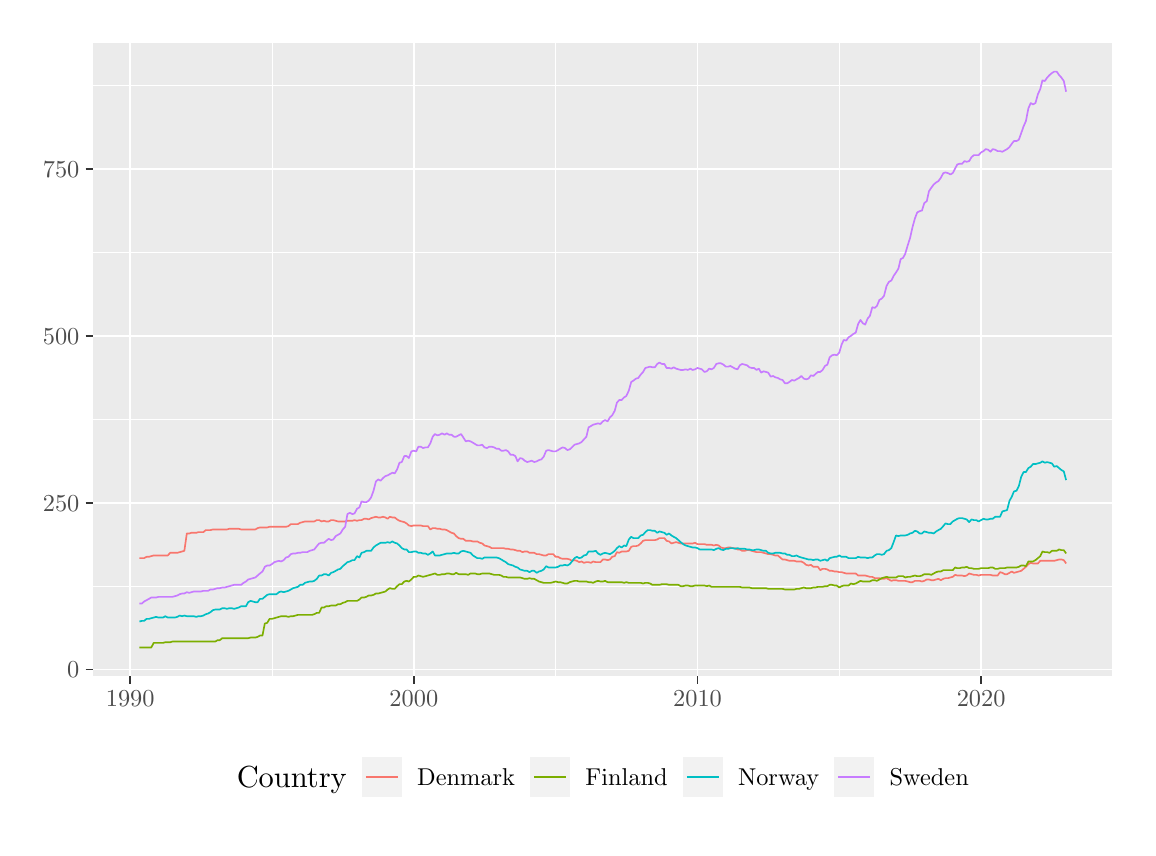
\begin{tikzpicture}[x=1pt,y=1pt]
\definecolor{fillColor}{RGB}{255,255,255}
\path[use as bounding box,fill=fillColor,fill opacity=0.00] (0,0) rectangle (397.48,289.08);
\begin{scope}
\path[clip] (  0.00,  0.00) rectangle (397.48,289.08);
\definecolor{drawColor}{RGB}{255,255,255}
\definecolor{fillColor}{RGB}{255,255,255}

\path[draw=drawColor,line width= 0.6pt,line join=round,line cap=round,fill=fillColor] (  0.00,  0.00) rectangle (397.48,289.08);
\end{scope}
\begin{scope}
\path[clip] ( 23.65, 54.68) rectangle (391.98,283.58);
\definecolor{fillColor}{gray}{0.92}

\path[fill=fillColor] ( 23.65, 54.68) rectangle (391.98,283.58);
\definecolor{drawColor}{RGB}{255,255,255}

\path[draw=drawColor,line width= 0.3pt,line join=round] ( 23.65, 87.26) --
	(391.98, 87.26);

\path[draw=drawColor,line width= 0.3pt,line join=round] ( 23.65,147.55) --
	(391.98,147.55);

\path[draw=drawColor,line width= 0.3pt,line join=round] ( 23.65,207.83) --
	(391.98,207.83);

\path[draw=drawColor,line width= 0.3pt,line join=round] ( 23.65,268.11) --
	(391.98,268.11);

\path[draw=drawColor,line width= 0.3pt,line join=round] ( 88.29, 54.68) --
	( 88.29,283.58);

\path[draw=drawColor,line width= 0.3pt,line join=round] (190.80, 54.68) --
	(190.80,283.58);

\path[draw=drawColor,line width= 0.3pt,line join=round] (293.30, 54.68) --
	(293.30,283.58);

\path[draw=drawColor,line width= 0.6pt,line join=round] ( 23.65, 57.12) --
	(391.98, 57.12);

\path[draw=drawColor,line width= 0.6pt,line join=round] ( 23.65,117.41) --
	(391.98,117.41);

\path[draw=drawColor,line width= 0.6pt,line join=round] ( 23.65,177.69) --
	(391.98,177.69);

\path[draw=drawColor,line width= 0.6pt,line join=round] ( 23.65,237.97) --
	(391.98,237.97);

\path[draw=drawColor,line width= 0.6pt,line join=round] ( 37.05, 54.68) --
	( 37.05,283.58);

\path[draw=drawColor,line width= 0.6pt,line join=round] (139.54, 54.68) --
	(139.54,283.58);

\path[draw=drawColor,line width= 0.6pt,line join=round] (242.05, 54.68) --
	(242.05,283.58);

\path[draw=drawColor,line width= 0.6pt,line join=round] (344.54, 54.68) --
	(344.54,283.58);
\definecolor{drawColor}{RGB}{248,118,109}

\path[draw=drawColor,line width= 0.6pt,line join=round] ( 40.39, 97.39) --
	( 41.26, 97.39) --
	( 42.07, 97.39) --
	( 42.97, 97.87) --
	( 43.84, 97.87) --
	( 44.63, 98.12) --
	( 45.55, 98.36) --
	( 46.40, 98.36) --
	( 47.27, 98.36) --
	( 48.13, 98.36) --
	( 48.92, 98.36) --
	( 49.73, 98.36) --
	( 50.63, 98.36) --
	( 51.50, 99.32) --
	( 52.29, 99.32) --
	( 53.21, 99.32) --
	( 54.06, 99.32) --
	( 54.93, 99.56) --
	( 55.80, 99.80) --
	( 56.61,100.04) --
	( 57.51,106.31) --
	( 58.38,106.31) --
	( 59.16,106.55) --
	( 60.06,106.55) --
	( 60.90,106.55) --
	( 61.72,106.80) --
	( 62.62,106.80) --
	( 63.49,106.80) --
	( 64.36,107.52) --
	( 65.20,107.52) --
	( 66.04,107.52) --
	( 66.91,107.76) --
	( 67.78,107.76) --
	( 68.59,107.76) --
	( 69.38,107.76) --
	( 70.31,107.76) --
	( 71.15,107.76) --
	( 72.02,107.76) --
	( 72.86,108.00) --
	( 73.70,108.00) --
	( 74.60,108.00) --
	( 75.44,108.00) --
	( 76.25,108.00) --
	( 77.15,107.76) --
	( 78.02,107.76) --
	( 78.89,107.76) --
	( 79.68,107.76) --
	( 80.55,107.76) --
	( 81.36,107.76) --
	( 82.26,107.76) --
	( 83.10,108.24) --
	( 83.92,108.48) --
	( 84.84,108.48) --
	( 85.68,108.48) --
	( 86.55,108.48) --
	( 87.40,108.72) --
	( 88.24,108.72) --
	( 89.14,108.72) --
	( 89.92,108.72) --
	( 90.79,108.72) --
	( 91.58,108.72) --
	( 92.50,108.72) --
	( 93.35,108.72) --
	( 94.22,108.97) --
	( 95.09,109.69) --
	( 95.90,109.69) --
	( 96.80,109.69) --
	( 97.64,109.69) --
	( 98.45,110.17) --
	( 99.38,110.41) --
	(100.19,110.65) --
	(101.01,110.65) --
	(101.90,110.65) --
	(102.77,110.65) --
	(103.56,110.65) --
	(104.49,111.14) --
	(105.33,111.14) --
	(106.20,110.65) --
	(107.07,110.89) --
	(107.88,110.65) --
	(108.78,110.65) --
	(109.65,111.14) --
	(110.44,111.14) --
	(111.31,110.89) --
	(112.15,110.65) --
	(112.99,110.65) --
	(113.86,110.65) --
	(114.73,110.65) --
	(115.54,110.89) --
	(116.44,110.89) --
	(117.31,110.89) --
	(118.10,111.14) --
	(119.02,110.89) --
	(119.87,111.14) --
	(120.65,111.14) --
	(121.55,111.62) --
	(122.39,111.62) --
	(123.20,111.38) --
	(124.10,111.86) --
	(124.97,112.10) --
	(125.84,112.34) --
	(126.68,112.10) --
	(127.53,112.10) --
	(128.40,112.34) --
	(129.27,112.10) --
	(130.08,111.62) --
	(130.87,112.34) --
	(131.79,112.10) --
	(132.63,112.10) --
	(133.50,111.38) --
	(134.35,110.89) --
	(135.19,110.65) --
	(136.09,110.41) --
	(136.93,109.93) --
	(137.74,109.21) --
	(138.64,108.97) --
	(139.51,109.21) --
	(140.38,109.21) --
	(141.19,109.21) --
	(142.06,109.21) --
	(142.85,108.97) --
	(143.78,108.97) --
	(144.62,108.97) --
	(145.49,107.76) --
	(146.36,108.24) --
	(147.17,108.24) --
	(148.07,108.00) --
	(148.91,108.00) --
	(149.72,107.76) --
	(150.65,107.76) --
	(151.44,107.52) --
	(152.28,107.04) --
	(153.15,106.55) --
	(154.02,106.31) --
	(154.83,105.35) --
	(155.73,104.63) --
	(156.60,104.38) --
	(157.39,104.38) --
	(158.31,103.66) --
	(159.15,103.66) --
	(160.02,103.66) --
	(160.89,103.42) --
	(161.68,103.42) --
	(162.49,103.42) --
	(163.39,102.94) --
	(164.26,102.70) --
	(165.05,101.97) --
	(165.97,101.73) --
	(166.82,101.49) --
	(167.69,101.01) --
	(168.56,101.01) --
	(169.37,101.01) --
	(170.27,101.01) --
	(171.14,101.01) --
	(171.92,101.01) --
	(172.79,100.77) --
	(173.63,100.77) --
	(174.48,100.53) --
	(175.35,100.53) --
	(176.22,100.29) --
	(177.03,100.04) --
	(177.93,100.04) --
	(178.80, 99.56) --
	(179.58, 99.80) --
	(180.51, 99.80) --
	(181.35, 99.32) --
	(182.14, 99.32) --
	(183.06, 99.32) --
	(183.91, 98.84) --
	(184.78, 98.84) --
	(185.62, 98.60) --
	(186.46, 98.36) --
	(187.36, 98.36) --
	(188.20, 98.84) --
	(189.01, 98.84) --
	(189.91, 98.84) --
	(190.78, 97.87) --
	(191.65, 97.87) --
	(192.44, 97.39) --
	(193.31, 97.15) --
	(194.12, 97.15) --
	(195.02, 97.15) --
	(195.86, 96.91) --
	(196.67, 96.43) --
	(197.60, 96.67) --
	(198.44, 96.43) --
	(199.31, 95.94) --
	(200.15, 96.19) --
	(201.00, 95.70) --
	(201.89, 95.94) --
	(202.68, 95.94) --
	(203.55, 95.70) --
	(204.34, 96.19) --
	(205.26, 95.94) --
	(206.10, 95.94) --
	(206.97, 95.94) --
	(207.84, 96.91) --
	(208.66, 96.91) --
	(209.56, 96.67) --
	(210.40, 96.91) --
	(211.21, 97.87) --
	(212.14, 98.12) --
	(212.92, 99.56) --
	(213.77, 99.32) --
	(214.64, 99.80) --
	(215.51, 99.80) --
	(216.32, 99.80) --
	(217.22,100.04) --
	(218.09,101.49) --
	(218.87,101.73) --
	(219.80,101.73) --
	(220.64,101.97) --
	(221.51,102.70) --
	(222.38,103.66) --
	(223.19,103.90) --
	(224.06,103.90) --
	(224.91,103.90) --
	(225.75,103.90) --
	(226.62,103.90) --
	(227.49,104.14) --
	(228.30,104.63) --
	(229.20,104.63) --
	(230.07,104.63) --
	(230.86,103.66) --
	(231.78,103.42) --
	(232.62,102.70) --
	(233.41,102.94) --
	(234.31,103.18) --
	(235.15,102.94) --
	(235.96,102.70) --
	(236.86,102.70) --
	(237.73,102.70) --
	(238.60,102.70) --
	(239.44,102.70) --
	(240.29,102.70) --
	(241.16,102.94) --
	(242.03,102.46) --
	(242.84,102.46) --
	(243.62,102.46) --
	(244.55,102.46) --
	(245.39,102.21) --
	(246.26,102.21) --
	(247.10,102.21) --
	(247.95,101.97) --
	(248.84,102.21) --
	(249.69,101.97) --
	(250.50,101.25) --
	(251.40,101.01) --
	(252.27,101.01) --
	(253.14,101.25) --
	(253.92,101.25) --
	(254.79,101.01) --
	(255.61,101.01) --
	(256.51,100.53) --
	(257.35,100.53) --
	(258.16,100.04) --
	(259.09,100.04) --
	(259.93,100.29) --
	(260.80,100.29) --
	(261.64,100.04) --
	(262.48, 99.80) --
	(263.38, 99.56) --
	(264.20, 99.56) --
	(265.04, 99.56) --
	(265.91, 99.32) --
	(266.78, 99.08) --
	(267.59, 98.84) --
	(268.49, 98.84) --
	(269.36, 98.60) --
	(270.14, 98.36) --
	(271.07, 98.36) --
	(271.91, 97.63) --
	(272.78, 96.91) --
	(273.65, 96.91) --
	(274.44, 96.67) --
	(275.25, 96.43) --
	(276.15, 96.43) --
	(277.02, 96.43) --
	(277.81, 96.19) --
	(278.73, 96.19) --
	(279.57, 96.19) --
	(280.44, 95.70) --
	(281.31, 94.98) --
	(282.13, 94.74) --
	(283.03, 94.98) --
	(283.90, 94.26) --
	(284.68, 94.26) --
	(285.55, 94.26) --
	(286.39, 93.05) --
	(287.24, 93.53) --
	(288.11, 93.53) --
	(288.98, 93.29) --
	(289.79, 92.81) --
	(290.69, 92.81) --
	(291.56, 92.57) --
	(292.34, 92.57) --
	(293.27, 92.33) --
	(294.11, 92.33) --
	(294.90, 92.09) --
	(295.79, 91.85) --
	(296.64, 91.85) --
	(297.45, 91.85) --
	(298.35, 91.85) --
	(299.22, 91.85) --
	(300.09, 91.12) --
	(300.93, 91.12) --
	(301.77, 91.12) --
	(302.64, 91.12) --
	(303.51, 90.88) --
	(304.33, 90.64) --
	(305.20, 90.64) --
	(306.07, 90.16) --
	(306.88, 90.16) --
	(307.78, 90.16) --
	(308.62, 89.92) --
	(309.43, 89.92) --
	(310.36, 90.16) --
	(311.20, 89.68) --
	(312.07, 89.19) --
	(312.91, 89.43) --
	(313.76, 89.43) --
	(314.65, 89.19) --
	(315.44, 89.19) --
	(316.31, 89.19) --
	(317.09, 89.19) --
	(318.02, 88.95) --
	(318.86, 88.71) --
	(319.73, 88.71) --
	(320.60, 89.19) --
	(321.42, 89.19) --
	(322.31, 89.19) --
	(323.16, 88.95) --
	(323.97, 89.19) --
	(324.90, 89.68) --
	(325.68, 89.68) --
	(326.52, 89.43) --
	(327.39, 89.43) --
	(328.26, 89.68) --
	(329.08, 89.92) --
	(329.98, 89.43) --
	(330.85, 89.92) --
	(331.63, 90.16) --
	(332.56, 90.16) --
	(333.40, 90.40) --
	(334.27, 90.64) --
	(335.14, 91.36) --
	(335.93, 91.12) --
	(336.74, 91.12) --
	(337.64, 91.12) --
	(338.51, 90.88) --
	(339.29, 91.12) --
	(340.22, 91.85) --
	(341.06, 91.60) --
	(341.93, 91.36) --
	(342.80, 91.36) --
	(343.61, 91.12) --
	(344.51, 91.36) --
	(345.38, 91.36) --
	(346.17, 91.36) --
	(347.07, 91.36) --
	(347.91, 91.36) --
	(348.72, 91.12) --
	(349.62, 91.12) --
	(350.49, 91.12) --
	(351.36, 92.33) --
	(352.20, 92.09) --
	(353.04, 91.60) --
	(353.91, 91.60) --
	(354.78, 92.09) --
	(355.60, 92.57) --
	(356.38, 92.09) --
	(357.31, 92.33) --
	(358.15, 92.57) --
	(359.02, 92.81) --
	(359.86, 93.53) --
	(360.71, 94.26) --
	(361.60, 95.22) --
	(362.45, 95.70) --
	(363.26, 95.46) --
	(364.16, 95.46) --
	(365.03, 95.46) --
	(365.90, 96.43) --
	(366.68, 96.43) --
	(367.55, 96.43) --
	(368.37, 96.43) --
	(369.26, 96.43) --
	(370.11, 96.43) --
	(370.92, 96.43) --
	(371.85, 96.67) --
	(372.69, 96.91) --
	(373.56, 96.91) --
	(374.40, 96.67) --
	(375.24, 95.46);
\definecolor{drawColor}{RGB}{124,174,0}

\path[draw=drawColor,line width= 0.6pt,line join=round] ( 40.39, 65.08) --
	( 41.26, 65.08) --
	( 42.07, 65.08) --
	( 42.97, 65.08) --
	( 43.84, 65.08) --
	( 44.63, 65.08) --
	( 45.55, 66.77) --
	( 46.40, 66.77) --
	( 47.27, 66.77) --
	( 48.13, 66.77) --
	( 48.92, 66.77) --
	( 49.73, 67.01) --
	( 50.63, 67.01) --
	( 51.50, 67.01) --
	( 52.29, 67.25) --
	( 53.21, 67.25) --
	( 54.06, 67.25) --
	( 54.93, 67.25) --
	( 55.80, 67.25) --
	( 56.61, 67.25) --
	( 57.51, 67.25) --
	( 58.38, 67.25) --
	( 59.16, 67.25) --
	( 60.06, 67.25) --
	( 60.90, 67.25) --
	( 61.72, 67.25) --
	( 62.62, 67.25) --
	( 63.49, 67.25) --
	( 64.36, 67.25) --
	( 65.20, 67.25) --
	( 66.04, 67.25) --
	( 66.91, 67.25) --
	( 67.78, 67.25) --
	( 68.59, 67.73) --
	( 69.38, 67.73) --
	( 70.31, 68.46) --
	( 71.15, 68.46) --
	( 72.02, 68.46) --
	( 72.86, 68.46) --
	( 73.70, 68.46) --
	( 74.60, 68.46) --
	( 75.44, 68.46) --
	( 76.25, 68.46) --
	( 77.15, 68.46) --
	( 78.02, 68.46) --
	( 78.89, 68.46) --
	( 79.68, 68.46) --
	( 80.55, 68.70) --
	( 81.36, 68.70) --
	( 82.26, 68.70) --
	( 83.10, 68.94) --
	( 83.92, 69.42) --
	( 84.84, 69.42) --
	( 85.68, 73.76) --
	( 86.55, 74.00) --
	( 87.40, 75.45) --
	( 88.24, 75.45) --
	( 89.14, 75.69) --
	( 89.92, 75.93) --
	( 90.79, 76.17) --
	( 91.58, 76.41) --
	( 92.50, 76.41) --
	( 93.35, 76.41) --
	( 94.22, 76.17) --
	( 95.09, 76.41) --
	( 95.90, 76.41) --
	( 96.80, 76.65) --
	( 97.64, 76.90) --
	( 98.45, 76.90) --
	( 99.38, 76.90) --
	(100.19, 76.90) --
	(101.01, 76.90) --
	(101.90, 76.90) --
	(102.77, 76.90) --
	(103.56, 77.14) --
	(104.49, 77.62) --
	(105.33, 77.62) --
	(106.20, 79.55) --
	(107.07, 79.55) --
	(107.88, 80.03) --
	(108.78, 80.03) --
	(109.65, 80.27) --
	(110.44, 80.27) --
	(111.31, 80.27) --
	(112.15, 80.75) --
	(112.99, 80.75) --
	(113.86, 81.24) --
	(114.73, 81.48) --
	(115.54, 81.96) --
	(116.44, 81.96) --
	(117.31, 81.96) --
	(118.10, 81.96) --
	(119.02, 81.96) --
	(119.87, 82.44) --
	(120.65, 83.16) --
	(121.55, 83.16) --
	(122.39, 83.41) --
	(123.20, 83.89) --
	(124.10, 83.89) --
	(124.97, 84.13) --
	(125.84, 84.61) --
	(126.68, 84.61) --
	(127.53, 84.85) --
	(128.40, 85.09) --
	(129.27, 85.34) --
	(130.08, 86.06) --
	(130.87, 86.54) --
	(131.79, 86.30) --
	(132.63, 86.30) --
	(133.50, 87.26) --
	(134.35, 87.99) --
	(135.19, 87.99) --
	(136.09, 88.95) --
	(136.93, 89.19) --
	(137.74, 88.95) --
	(138.64, 89.68) --
	(139.51, 90.64) --
	(140.38, 90.64) --
	(141.19, 91.12) --
	(142.06, 90.88) --
	(142.85, 90.64) --
	(143.78, 90.88) --
	(144.62, 91.12) --
	(145.49, 91.36) --
	(146.36, 91.60) --
	(147.17, 91.85) --
	(148.07, 91.36) --
	(148.91, 91.36) --
	(149.72, 91.60) --
	(150.65, 91.60) --
	(151.44, 91.85) --
	(152.28, 91.85) --
	(153.15, 91.60) --
	(154.02, 91.60) --
	(154.83, 92.09) --
	(155.73, 91.60) --
	(156.60, 91.60) --
	(157.39, 91.60) --
	(158.31, 91.60) --
	(159.15, 91.36) --
	(160.02, 91.85) --
	(160.89, 91.85) --
	(161.68, 91.85) --
	(162.49, 91.60) --
	(163.39, 91.60) --
	(164.26, 91.85) --
	(165.05, 91.85) --
	(165.97, 91.85) --
	(166.82, 91.85) --
	(167.69, 91.60) --
	(168.56, 91.36) --
	(169.37, 91.36) --
	(170.27, 91.36) --
	(171.14, 91.12) --
	(171.92, 90.64) --
	(172.79, 90.64) --
	(173.63, 90.40) --
	(174.48, 90.40) --
	(175.35, 90.40) --
	(176.22, 90.40) --
	(177.03, 90.40) --
	(177.93, 90.40) --
	(178.80, 90.16) --
	(179.58, 89.92) --
	(180.51, 89.92) --
	(181.35, 90.16) --
	(182.14, 89.92) --
	(183.06, 89.92) --
	(183.91, 89.43) --
	(184.78, 88.95) --
	(185.62, 88.71) --
	(186.46, 88.47) --
	(187.36, 88.47) --
	(188.20, 88.47) --
	(189.01, 88.47) --
	(189.91, 88.71) --
	(190.78, 88.95) --
	(191.65, 88.71) --
	(192.44, 88.71) --
	(193.31, 88.47) --
	(194.12, 88.23) --
	(195.02, 88.23) --
	(195.86, 88.71) --
	(196.67, 88.95) --
	(197.60, 89.19) --
	(198.44, 89.19) --
	(199.31, 88.95) --
	(200.15, 88.95) --
	(201.00, 88.95) --
	(201.89, 88.95) --
	(202.68, 88.71) --
	(203.55, 88.71) --
	(204.34, 88.47) --
	(205.26, 88.95) --
	(206.10, 89.19) --
	(206.97, 88.95) --
	(207.84, 88.95) --
	(208.66, 89.19) --
	(209.56, 88.71) --
	(210.40, 88.71) --
	(211.21, 88.71) --
	(212.14, 88.71) --
	(212.92, 88.71) --
	(213.77, 88.71) --
	(214.64, 88.71) --
	(215.51, 88.47) --
	(216.32, 88.71) --
	(217.22, 88.47) --
	(218.09, 88.47) --
	(218.87, 88.47) --
	(219.80, 88.47) --
	(220.64, 88.47) --
	(221.51, 88.47) --
	(222.38, 88.23) --
	(223.19, 88.47) --
	(224.06, 88.47) --
	(224.91, 88.23) --
	(225.75, 87.75) --
	(226.62, 87.75) --
	(227.49, 87.75) --
	(228.30, 87.75) --
	(229.20, 87.99) --
	(230.07, 87.99) --
	(230.86, 87.99) --
	(231.78, 87.75) --
	(232.62, 87.75) --
	(233.41, 87.75) --
	(234.31, 87.75) --
	(235.15, 87.75) --
	(235.96, 87.26) --
	(236.86, 87.26) --
	(237.73, 87.51) --
	(238.60, 87.51) --
	(239.44, 87.26) --
	(240.29, 87.26) --
	(241.16, 87.51) --
	(242.03, 87.51) --
	(242.84, 87.51) --
	(243.62, 87.51) --
	(244.55, 87.51) --
	(245.39, 87.26) --
	(246.26, 87.51) --
	(247.10, 87.02) --
	(247.95, 87.02) --
	(248.84, 87.02) --
	(249.69, 87.02) --
	(250.50, 87.02) --
	(251.40, 87.02) --
	(252.27, 87.02) --
	(253.14, 87.02) --
	(253.92, 87.02) --
	(254.79, 87.02) --
	(255.61, 87.02) --
	(256.51, 87.02) --
	(257.35, 87.02) --
	(258.16, 86.78) --
	(259.09, 86.78) --
	(259.93, 86.78) --
	(260.80, 86.78) --
	(261.64, 86.54) --
	(262.48, 86.54) --
	(263.38, 86.54) --
	(264.20, 86.54) --
	(265.04, 86.54) --
	(265.91, 86.54) --
	(266.78, 86.54) --
	(267.59, 86.30) --
	(268.49, 86.30) --
	(269.36, 86.30) --
	(270.14, 86.30) --
	(271.07, 86.30) --
	(271.91, 86.30) --
	(272.78, 86.30) --
	(273.65, 86.06) --
	(274.44, 86.06) --
	(275.25, 86.06) --
	(276.15, 86.06) --
	(277.02, 86.06) --
	(277.81, 86.30) --
	(278.73, 86.30) --
	(279.57, 86.54) --
	(280.44, 86.78) --
	(281.31, 86.54) --
	(282.13, 86.54) --
	(283.03, 86.54) --
	(283.90, 86.78) --
	(284.68, 86.78) --
	(285.55, 87.02) --
	(286.39, 87.02) --
	(287.24, 87.02) --
	(288.11, 87.26) --
	(288.98, 87.26) --
	(289.79, 87.75) --
	(290.69, 87.75) --
	(291.56, 87.51) --
	(292.34, 87.51) --
	(293.27, 86.78) --
	(294.11, 87.26) --
	(294.90, 87.51) --
	(295.79, 87.51) --
	(296.64, 87.51) --
	(297.45, 88.23) --
	(298.35, 87.99) --
	(299.22, 88.23) --
	(300.09, 88.71) --
	(300.93, 89.19) --
	(301.77, 88.95) --
	(302.64, 88.95) --
	(303.51, 88.95) --
	(304.33, 88.95) --
	(305.20, 89.43) --
	(306.07, 89.43) --
	(306.88, 89.19) --
	(307.78, 89.68) --
	(308.62, 90.16) --
	(309.43, 90.40) --
	(310.36, 90.64) --
	(311.20, 90.40) --
	(312.07, 90.40) --
	(312.91, 90.40) --
	(313.76, 90.40) --
	(314.65, 90.88) --
	(315.44, 90.88) --
	(316.31, 90.88) --
	(317.09, 90.40) --
	(318.02, 90.64) --
	(318.86, 90.64) --
	(319.73, 90.88) --
	(320.60, 91.12) --
	(321.42, 90.88) --
	(322.31, 90.88) --
	(323.16, 91.12) --
	(323.97, 91.60) --
	(324.90, 91.60) --
	(325.68, 91.60) --
	(326.52, 91.36) --
	(327.39, 91.85) --
	(328.26, 92.33) --
	(329.08, 92.57) --
	(329.98, 92.57) --
	(330.85, 93.05) --
	(331.63, 93.05) --
	(332.56, 93.05) --
	(333.40, 93.05) --
	(334.27, 93.05) --
	(335.14, 94.02) --
	(335.93, 93.77) --
	(336.74, 93.77) --
	(337.64, 94.02) --
	(338.51, 94.02) --
	(339.29, 94.26) --
	(340.22, 93.77) --
	(341.06, 93.77) --
	(341.93, 93.53) --
	(342.80, 93.53) --
	(343.61, 93.53) --
	(344.51, 93.77) --
	(345.38, 93.77) --
	(346.17, 93.77) --
	(347.07, 93.77) --
	(347.91, 94.02) --
	(348.72, 94.02) --
	(349.62, 93.53) --
	(350.49, 93.53) --
	(351.36, 93.77) --
	(352.20, 93.77) --
	(353.04, 93.77) --
	(353.91, 94.02) --
	(354.78, 94.02) --
	(355.60, 94.02) --
	(356.38, 94.02) --
	(357.31, 94.02) --
	(358.15, 94.26) --
	(359.02, 94.74) --
	(359.86, 94.74) --
	(360.71, 94.50) --
	(361.60, 96.19) --
	(362.45, 96.19) --
	(363.26, 96.19) --
	(364.16, 96.67) --
	(365.03, 97.39) --
	(365.90, 98.12) --
	(366.68, 99.80) --
	(367.55, 99.56) --
	(368.37, 99.56) --
	(369.26, 99.32) --
	(370.11,100.04) --
	(370.92,100.04) --
	(371.85,100.04) --
	(372.69,100.53) --
	(373.56,100.29) --
	(374.40,100.29) --
	(375.24, 99.08);
\definecolor{drawColor}{RGB}{0,191,196}

\path[draw=drawColor,line width= 0.6pt,line join=round] ( 40.39, 74.48) --
	( 41.26, 74.73) --
	( 42.07, 74.73) --
	( 42.97, 75.45) --
	( 43.84, 75.45) --
	( 44.63, 75.69) --
	( 45.55, 75.93) --
	( 46.40, 76.17) --
	( 47.27, 75.93) --
	( 48.13, 75.93) --
	( 48.92, 75.93) --
	( 49.73, 76.41) --
	( 50.63, 75.93) --
	( 51.50, 75.93) --
	( 52.29, 75.93) --
	( 53.21, 75.93) --
	( 54.06, 76.17) --
	( 54.93, 76.65) --
	( 55.80, 76.41) --
	( 56.61, 76.65) --
	( 57.51, 76.41) --
	( 58.38, 76.41) --
	( 59.16, 76.41) --
	( 60.06, 76.41) --
	( 60.90, 76.17) --
	( 61.72, 76.41) --
	( 62.62, 76.41) --
	( 63.49, 76.65) --
	( 64.36, 77.14) --
	( 65.20, 77.38) --
	( 66.04, 77.86) --
	( 66.91, 78.58) --
	( 67.78, 78.82) --
	( 68.59, 78.82) --
	( 69.38, 78.82) --
	( 70.31, 79.31) --
	( 71.15, 79.31) --
	( 72.02, 79.07) --
	( 72.86, 79.31) --
	( 73.70, 79.31) --
	( 74.60, 79.07) --
	( 75.44, 79.31) --
	( 76.25, 79.55) --
	( 77.15, 80.03) --
	( 78.02, 80.03) --
	( 78.89, 80.03) --
	( 79.68, 81.48) --
	( 80.55, 81.96) --
	( 81.36, 81.72) --
	( 82.26, 81.48) --
	( 83.10, 81.48) --
	( 83.92, 82.68) --
	( 84.84, 82.68) --
	( 85.68, 83.41) --
	( 86.55, 84.13) --
	( 87.40, 84.37) --
	( 88.24, 84.37) --
	( 89.14, 84.37) --
	( 89.92, 84.37) --
	( 90.79, 85.09) --
	( 91.58, 85.34) --
	( 92.50, 85.09) --
	( 93.35, 85.34) --
	( 94.22, 85.58) --
	( 95.09, 86.06) --
	( 95.90, 86.54) --
	( 96.80, 86.78) --
	( 97.64, 87.02) --
	( 98.45, 87.75) --
	( 99.38, 87.75) --
	(100.19, 88.47) --
	(101.01, 88.71) --
	(101.90, 88.95) --
	(102.77, 88.95) --
	(103.56, 89.19) --
	(104.49, 89.92) --
	(105.33, 91.12) --
	(106.20, 91.12) --
	(107.07, 91.60) --
	(107.88, 91.60) --
	(108.78, 91.12) --
	(109.65, 92.09) --
	(110.44, 92.33) --
	(111.31, 92.81) --
	(112.15, 93.29) --
	(112.99, 93.53) --
	(113.86, 94.50) --
	(114.73, 95.22) --
	(115.54, 95.94) --
	(116.44, 96.19) --
	(117.31, 96.67) --
	(118.10, 96.67) --
	(119.02, 98.12) --
	(119.87, 97.63) --
	(120.65, 99.32) --
	(121.55, 99.56) --
	(122.39,100.04) --
	(123.20,100.04) --
	(124.10,100.04) --
	(124.97,101.25) --
	(125.84,101.97) --
	(126.68,102.46) --
	(127.53,102.94) --
	(128.40,102.94) --
	(129.27,102.94) --
	(130.08,103.18) --
	(130.87,102.94) --
	(131.79,103.42) --
	(132.63,102.94) --
	(133.50,102.70) --
	(134.35,101.97) --
	(135.19,101.01) --
	(136.09,100.53) --
	(136.93,100.53) --
	(137.74, 99.56) --
	(138.64, 99.56) --
	(139.51, 99.80) --
	(140.38, 99.80) --
	(141.19, 99.32) --
	(142.06, 99.32) --
	(142.85, 99.08) --
	(143.78, 99.08) --
	(144.62, 98.60) --
	(145.49, 99.08) --
	(146.36, 99.80) --
	(147.17, 98.36) --
	(148.07, 98.36) --
	(148.91, 98.36) --
	(149.72, 98.60) --
	(150.65, 98.84) --
	(151.44, 99.08) --
	(152.28, 99.08) --
	(153.15, 99.08) --
	(154.02, 99.32) --
	(154.83, 99.08) --
	(155.73, 99.08) --
	(156.60, 99.80) --
	(157.39,100.04) --
	(158.31, 99.80) --
	(159.15, 99.56) --
	(160.02, 99.32) --
	(160.89, 98.36) --
	(161.68, 97.87) --
	(162.49, 97.39) --
	(163.39, 97.39) --
	(164.26, 97.15) --
	(165.05, 97.63) --
	(165.97, 97.63) --
	(166.82, 97.63) --
	(167.69, 97.63) --
	(168.56, 97.63) --
	(169.37, 97.63) --
	(170.27, 97.39) --
	(171.14, 96.91) --
	(171.92, 96.43) --
	(172.79, 95.94) --
	(173.63, 95.22) --
	(174.48, 94.98) --
	(175.35, 94.74) --
	(176.22, 94.26) --
	(177.03, 94.02) --
	(177.93, 93.29) --
	(178.80, 93.05) --
	(179.58, 92.81) --
	(180.51, 92.81) --
	(181.35, 92.33) --
	(182.14, 92.81) --
	(183.06, 92.81) --
	(183.91, 92.09) --
	(184.78, 92.57) --
	(185.62, 92.81) --
	(186.46, 93.29) --
	(187.36, 94.50) --
	(188.20, 94.02) --
	(189.01, 94.02) --
	(189.91, 94.02) --
	(190.78, 94.02) --
	(191.65, 94.26) --
	(192.44, 94.74) --
	(193.31, 94.74) --
	(194.12, 94.98) --
	(195.02, 94.74) --
	(195.86, 95.22) --
	(196.67, 96.19) --
	(197.60, 97.39) --
	(198.44, 97.87) --
	(199.31, 97.39) --
	(200.15, 97.63) --
	(201.00, 98.36) --
	(201.89, 98.60) --
	(202.68, 99.80) --
	(203.55, 99.80) --
	(204.34, 99.80) --
	(205.26,100.04) --
	(206.10, 99.08) --
	(206.97, 98.60) --
	(207.84, 99.08) --
	(208.66, 99.32) --
	(209.56, 99.08) --
	(210.40, 98.84) --
	(211.21, 99.32) --
	(212.14,100.04) --
	(212.92,101.01) --
	(213.77,101.73) --
	(214.64,101.25) --
	(215.51,101.97) --
	(216.32,101.73) --
	(217.22,104.14) --
	(218.09,105.11) --
	(218.87,104.63) --
	(219.80,104.63) --
	(220.64,104.63) --
	(221.51,105.59) --
	(222.38,105.83) --
	(223.19,106.80) --
	(224.06,107.52) --
	(224.91,107.52) --
	(225.75,107.28) --
	(226.62,107.28) --
	(227.49,106.55) --
	(228.30,107.04) --
	(229.20,106.80) --
	(230.07,106.55) --
	(230.86,105.83) --
	(231.78,106.31) --
	(232.62,105.59) --
	(233.41,105.11) --
	(234.31,104.63) --
	(235.15,103.90) --
	(235.96,103.18) --
	(236.86,102.46) --
	(237.73,101.97) --
	(238.60,101.73) --
	(239.44,101.49) --
	(240.29,101.25) --
	(241.16,101.25) --
	(242.03,101.01) --
	(242.84,100.53) --
	(243.62,100.53) --
	(244.55,100.53) --
	(245.39,100.53) --
	(246.26,100.53) --
	(247.10,100.53) --
	(247.95,100.29) --
	(248.84,100.77) --
	(249.69,101.01) --
	(250.50,100.53) --
	(251.40,100.29) --
	(252.27,100.77) --
	(253.14,100.77) --
	(253.92,101.01) --
	(254.79,101.01) --
	(255.61,100.77) --
	(256.51,101.01) --
	(257.35,100.77) --
	(258.16,100.77) --
	(259.09,100.77) --
	(259.93,100.53) --
	(260.80,100.53) --
	(261.64,100.29) --
	(262.48,100.29) --
	(263.38,100.53) --
	(264.20,100.53) --
	(265.04,100.29) --
	(265.91,100.04) --
	(266.78,100.04) --
	(267.59, 99.32) --
	(268.49, 99.08) --
	(269.36, 99.08) --
	(270.14, 99.32) --
	(271.07, 99.32) --
	(271.91, 99.32) --
	(272.78, 99.08) --
	(273.65, 99.08) --
	(274.44, 98.60) --
	(275.25, 98.60) --
	(276.15, 98.12) --
	(277.02, 98.12) --
	(277.81, 98.36) --
	(278.73, 97.87) --
	(279.57, 97.63) --
	(280.44, 97.39) --
	(281.31, 97.15) --
	(282.13, 96.91) --
	(283.03, 96.91) --
	(283.90, 96.67) --
	(284.68, 96.91) --
	(285.55, 96.91) --
	(286.39, 96.43) --
	(287.24, 96.67) --
	(288.11, 96.91) --
	(288.98, 96.43) --
	(289.79, 97.39) --
	(290.69, 97.63) --
	(291.56, 97.87) --
	(292.34, 97.87) --
	(293.27, 98.36) --
	(294.11, 97.87) --
	(294.90, 97.87) --
	(295.79, 97.87) --
	(296.64, 97.39) --
	(297.45, 97.39) --
	(298.35, 97.39) --
	(299.22, 97.39) --
	(300.09, 97.87) --
	(300.93, 97.63) --
	(301.77, 97.63) --
	(302.64, 97.63) --
	(303.51, 97.39) --
	(304.33, 97.63) --
	(305.20, 97.63) --
	(306.07, 98.36) --
	(306.88, 98.84) --
	(307.78, 98.84) --
	(308.62, 98.60) --
	(309.43, 98.84) --
	(310.36,100.04) --
	(311.20,100.29) --
	(312.07,101.01) --
	(312.91,103.18) --
	(313.76,105.59) --
	(314.65,105.35) --
	(315.44,105.59) --
	(316.31,105.59) --
	(317.09,105.59) --
	(318.02,105.83) --
	(318.86,106.31) --
	(319.73,106.55) --
	(320.60,107.28) --
	(321.42,107.04) --
	(322.31,106.31) --
	(323.16,106.31) --
	(323.97,107.04) --
	(324.90,106.80) --
	(325.68,106.55) --
	(326.52,106.55) --
	(327.39,106.31) --
	(328.26,107.04) --
	(329.08,107.52) --
	(329.98,108.00) --
	(330.85,108.97) --
	(331.63,109.93) --
	(332.56,109.69) --
	(333.40,109.69) --
	(334.27,110.65) --
	(335.14,111.14) --
	(335.93,111.62) --
	(336.74,111.86) --
	(337.64,111.86) --
	(338.51,111.62) --
	(339.29,111.38) --
	(340.22,110.41) --
	(341.06,111.38) --
	(341.93,111.14) --
	(342.80,111.14) --
	(343.61,110.65) --
	(344.51,111.14) --
	(345.38,111.62) --
	(346.17,111.38) --
	(347.07,111.38) --
	(347.91,111.62) --
	(348.72,111.62) --
	(349.62,112.34) --
	(350.49,112.34) --
	(351.36,112.34) --
	(352.20,114.27) --
	(353.04,114.51) --
	(353.91,114.75) --
	(354.78,118.13) --
	(355.60,119.58) --
	(356.38,121.50) --
	(357.31,121.75) --
	(358.15,123.43) --
	(359.02,126.81) --
	(359.86,128.50) --
	(360.71,128.50) --
	(361.60,129.94) --
	(362.45,130.43) --
	(363.26,131.39) --
	(364.16,131.39) --
	(365.03,131.63) --
	(365.90,131.87) --
	(366.68,132.36) --
	(367.55,131.87) --
	(368.37,132.11) --
	(369.26,131.87) --
	(370.11,131.63) --
	(370.92,130.43) --
	(371.85,130.67) --
	(372.69,129.94) --
	(373.56,129.22) --
	(374.40,128.74) --
	(375.24,125.60);
\definecolor{drawColor}{RGB}{199,124,255}

\path[draw=drawColor,line width= 0.6pt,line join=round] ( 40.39, 80.99) --
	( 41.26, 80.99) --
	( 42.07, 81.72) --
	( 42.97, 82.20) --
	( 43.84, 82.68) --
	( 44.63, 83.16) --
	( 45.55, 83.16) --
	( 46.40, 83.16) --
	( 47.27, 83.41) --
	( 48.13, 83.41) --
	( 48.92, 83.41) --
	( 49.73, 83.41) --
	( 50.63, 83.41) --
	( 51.50, 83.41) --
	( 52.29, 83.41) --
	( 53.21, 83.65) --
	( 54.06, 83.89) --
	( 54.93, 84.37) --
	( 55.80, 84.61) --
	( 56.61, 84.61) --
	( 57.51, 85.09) --
	( 58.38, 84.85) --
	( 59.16, 85.09) --
	( 60.06, 85.34) --
	( 60.90, 85.34) --
	( 61.72, 85.34) --
	( 62.62, 85.34) --
	( 63.49, 85.58) --
	( 64.36, 85.58) --
	( 65.20, 85.58) --
	( 66.04, 86.06) --
	( 66.91, 86.06) --
	( 67.78, 86.30) --
	( 68.59, 86.54) --
	( 69.38, 86.54) --
	( 70.31, 86.78) --
	( 71.15, 86.78) --
	( 72.02, 87.02) --
	( 72.86, 87.26) --
	( 73.70, 87.51) --
	( 74.60, 87.75) --
	( 75.44, 87.75) --
	( 76.25, 87.75) --
	( 77.15, 87.75) --
	( 78.02, 88.47) --
	( 78.89, 88.95) --
	( 79.68, 89.68) --
	( 80.55, 89.92) --
	( 81.36, 90.16) --
	( 82.26, 90.40) --
	( 83.10, 91.12) --
	( 83.92, 91.85) --
	( 84.84, 92.57) --
	( 85.68, 94.26) --
	( 86.55, 94.74) --
	( 87.40, 94.74) --
	( 88.24, 95.22) --
	( 89.14, 95.94) --
	( 89.92, 96.19) --
	( 90.79, 96.43) --
	( 91.58, 96.19) --
	( 92.50, 96.67) --
	( 93.35, 97.63) --
	( 94.22, 97.87) --
	( 95.09, 98.84) --
	( 95.90, 99.08) --
	( 96.80, 99.08) --
	( 97.64, 99.32) --
	( 98.45, 99.32) --
	( 99.38, 99.56) --
	(100.19, 99.56) --
	(101.01, 99.56) --
	(101.90,100.04) --
	(102.77,100.29) --
	(103.56,100.53) --
	(104.49,101.73) --
	(105.33,102.70) --
	(106.20,102.94) --
	(107.07,102.94) --
	(107.88,103.66) --
	(108.78,104.38) --
	(109.65,103.90) --
	(110.44,104.14) --
	(111.31,105.35) --
	(112.15,105.83) --
	(112.99,106.31) --
	(113.86,107.76) --
	(114.73,108.72) --
	(115.54,113.31) --
	(116.44,113.79) --
	(117.31,113.31) --
	(118.10,113.55) --
	(119.02,115.24) --
	(119.87,115.72) --
	(120.65,117.89) --
	(121.55,117.65) --
	(122.39,117.65) --
	(123.20,118.13) --
	(124.10,119.33) --
	(124.97,121.75) --
	(125.84,125.12) --
	(126.68,125.84) --
	(127.53,125.36) --
	(128.40,126.33) --
	(129.27,127.05) --
	(130.08,127.29) --
	(130.87,127.77) --
	(131.79,128.26) --
	(132.63,128.02) --
	(133.50,129.46) --
	(134.35,131.87) --
	(135.19,132.11) --
	(136.09,134.28) --
	(136.93,134.28) --
	(137.74,133.56) --
	(138.64,135.97) --
	(139.51,136.21) --
	(140.38,135.97) --
	(141.19,137.66) --
	(142.06,137.66) --
	(142.85,137.18) --
	(143.78,137.42) --
	(144.62,137.42) --
	(145.49,138.87) --
	(146.36,141.28) --
	(147.17,142.24) --
	(148.07,141.76) --
	(148.91,142.00) --
	(149.72,142.48) --
	(150.65,142.00) --
	(151.44,142.48) --
	(152.28,142.00) --
	(153.15,142.00) --
	(154.02,141.28) --
	(154.83,141.28) --
	(155.73,141.76) --
	(156.60,142.24) --
	(157.39,141.04) --
	(158.31,139.59) --
	(159.15,139.83) --
	(160.02,139.59) --
	(160.89,139.11) --
	(161.68,138.62) --
	(162.49,138.14) --
	(163.39,138.14) --
	(164.26,138.38) --
	(165.05,137.42) --
	(165.97,137.18) --
	(166.82,137.66) --
	(167.69,137.66) --
	(168.56,137.42) --
	(169.37,136.94) --
	(170.27,136.94) --
	(171.14,136.21) --
	(171.92,136.21) --
	(172.79,136.45) --
	(173.63,135.97) --
	(174.48,134.77) --
	(175.35,134.77) --
	(176.22,134.28) --
	(177.03,132.36) --
	(177.93,133.56) --
	(178.80,133.32) --
	(179.58,132.60) --
	(180.51,132.11) --
	(181.35,132.36) --
	(182.14,132.60) --
	(183.06,132.11) --
	(183.91,132.36) --
	(184.78,132.84) --
	(185.62,133.08) --
	(186.46,134.04) --
	(187.36,136.21) --
	(188.20,136.45) --
	(189.01,136.21) --
	(189.91,135.97) --
	(190.78,135.97) --
	(191.65,136.45) --
	(192.44,136.94) --
	(193.31,137.42) --
	(194.12,137.18) --
	(195.02,136.45) --
	(195.86,136.70) --
	(196.67,137.42) --
	(197.60,138.38) --
	(198.44,138.62) --
	(199.31,138.87) --
	(200.15,139.35) --
	(201.00,140.31) --
	(201.89,141.28) --
	(202.68,144.65) --
	(203.55,145.14) --
	(204.34,145.62) --
	(205.26,145.86) --
	(206.10,146.10) --
	(206.97,145.86) --
	(207.84,146.82) --
	(208.66,147.31) --
	(209.56,146.82) --
	(210.40,148.27) --
	(211.21,148.99) --
	(212.14,150.68) --
	(212.92,153.57) --
	(213.77,154.54) --
	(214.64,154.54) --
	(215.51,155.50) --
	(216.32,155.99) --
	(217.22,157.92) --
	(218.09,161.05) --
	(218.87,161.53) --
	(219.80,162.26) --
	(220.64,162.50) --
	(221.51,163.70) --
	(222.38,164.67) --
	(223.19,166.11) --
	(224.06,166.35) --
	(224.91,166.60) --
	(225.75,166.35) --
	(226.62,166.35) --
	(227.49,167.56) --
	(228.30,168.04) --
	(229.20,167.56) --
	(230.07,167.56) --
	(230.86,166.11) --
	(231.78,166.11) --
	(232.62,165.87) --
	(233.41,166.35) --
	(234.31,165.87) --
	(235.15,165.63) --
	(235.96,165.39) --
	(236.86,165.39) --
	(237.73,165.63) --
	(238.60,165.39) --
	(239.44,165.87) --
	(240.29,165.39) --
	(241.16,165.63) --
	(242.03,166.11) --
	(242.84,165.87) --
	(243.62,165.63) --
	(244.55,164.67) --
	(245.39,164.91) --
	(246.26,165.87) --
	(247.10,165.63) --
	(247.95,166.11) --
	(248.84,167.56) --
	(249.69,167.80) --
	(250.50,167.80) --
	(251.40,167.32) --
	(252.27,166.60) --
	(253.14,166.60) --
	(253.92,166.84) --
	(254.79,166.35) --
	(255.61,165.87) --
	(256.51,165.63) --
	(257.35,167.08) --
	(258.16,167.56) --
	(259.09,167.32) --
	(259.93,167.08) --
	(260.80,166.35) --
	(261.64,166.11) --
	(262.48,166.11) --
	(263.38,165.39) --
	(264.20,165.87) --
	(265.04,164.43) --
	(265.91,164.91) --
	(266.78,164.67) --
	(267.59,164.43) --
	(268.49,162.98) --
	(269.36,163.22) --
	(270.14,162.74) --
	(271.07,162.50) --
	(271.91,162.01) --
	(272.78,161.77) --
	(273.65,160.57) --
	(274.44,160.57) --
	(275.25,161.05) --
	(276.15,161.77) --
	(277.02,161.53) --
	(277.81,162.01) --
	(278.73,162.50) --
	(279.57,163.22) --
	(280.44,162.26) --
	(281.31,162.01) --
	(282.13,162.26) --
	(283.03,163.46) --
	(283.90,163.22) --
	(284.68,163.94) --
	(285.55,164.67) --
	(286.39,164.67) --
	(287.24,165.39) --
	(288.11,166.84) --
	(288.98,167.32) --
	(289.79,169.97) --
	(290.69,170.70) --
	(291.56,170.94) --
	(292.34,170.70) --
	(293.27,171.66) --
	(294.11,174.55) --
	(294.90,176.24) --
	(295.79,176.00) --
	(296.64,177.21) --
	(297.45,177.69) --
	(298.35,178.41) --
	(299.22,178.89) --
	(300.09,182.03) --
	(300.93,183.47) --
	(301.77,182.27) --
	(302.64,181.79) --
	(303.51,183.96) --
	(304.33,184.92) --
	(305.20,188.06) --
	(306.07,187.82) --
	(306.88,188.54) --
	(307.78,190.71) --
	(308.62,191.19) --
	(309.43,192.16) --
	(310.36,195.77) --
	(311.20,197.22) --
	(312.07,197.70) --
	(312.91,199.39) --
	(313.76,200.60) --
	(314.65,202.04) --
	(315.44,205.42) --
	(316.31,205.90) --
	(317.09,207.35) --
	(318.02,210.48) --
	(318.86,213.13) --
	(319.73,216.99) --
	(320.60,220.13) --
	(321.42,222.30) --
	(322.31,222.78) --
	(323.16,223.02) --
	(323.97,225.67) --
	(324.90,226.40) --
	(325.68,230.01) --
	(326.52,231.22) --
	(327.39,232.42) --
	(328.26,233.15) --
	(329.08,233.63) --
	(329.98,234.84) --
	(330.85,236.52) --
	(331.63,236.76) --
	(332.56,236.52) --
	(333.40,236.04) --
	(334.27,236.52) --
	(335.14,238.21) --
	(335.93,239.66) --
	(336.74,239.90) --
	(337.64,239.90) --
	(338.51,240.86) --
	(339.29,240.62) --
	(340.22,240.86) --
	(341.06,242.31) --
	(341.93,243.03) --
	(342.80,243.03) --
	(343.61,243.03) --
	(344.51,244.00) --
	(345.38,244.48) --
	(346.17,245.20) --
	(347.07,244.96) --
	(347.91,244.24) --
	(348.72,245.20) --
	(349.62,244.96) --
	(350.49,244.48) --
	(351.36,244.48) --
	(352.20,244.24) --
	(353.04,244.72) --
	(353.91,245.20) --
	(354.78,245.93) --
	(355.60,247.13) --
	(356.38,248.10) --
	(357.31,248.10) --
	(358.15,248.58) --
	(359.02,250.99) --
	(359.86,253.40) --
	(360.71,255.33) --
	(361.60,259.91) --
	(362.45,261.84) --
	(363.26,261.36) --
	(364.16,261.84) --
	(365.03,264.98) --
	(365.90,266.91) --
	(366.68,270.04) --
	(367.55,269.80) --
	(368.37,271.01) --
	(369.26,271.97) --
	(370.11,272.69) --
	(370.92,273.18) --
	(371.85,273.18) --
	(372.69,271.97) --
	(373.56,271.01) --
	(374.40,269.80) --
	(375.24,265.94);
\end{scope}
\begin{scope}
\path[clip] (  0.00,  0.00) rectangle (397.48,289.08);
\definecolor{drawColor}{gray}{0.30}

\node[text=drawColor,anchor=base east,inner sep=0pt, outer sep=0pt, scale=  0.88] at ( 18.70, 54.09) {0};

\node[text=drawColor,anchor=base east,inner sep=0pt, outer sep=0pt, scale=  0.88] at ( 18.70,114.38) {250};

\node[text=drawColor,anchor=base east,inner sep=0pt, outer sep=0pt, scale=  0.88] at ( 18.70,174.66) {500};

\node[text=drawColor,anchor=base east,inner sep=0pt, outer sep=0pt, scale=  0.88] at ( 18.70,234.94) {750};
\end{scope}
\begin{scope}
\path[clip] (  0.00,  0.00) rectangle (397.48,289.08);
\definecolor{drawColor}{gray}{0.20}

\path[draw=drawColor,line width= 0.6pt,line join=round] ( 20.90, 57.12) --
	( 23.65, 57.12);

\path[draw=drawColor,line width= 0.6pt,line join=round] ( 20.90,117.41) --
	( 23.65,117.41);

\path[draw=drawColor,line width= 0.6pt,line join=round] ( 20.90,177.69) --
	( 23.65,177.69);

\path[draw=drawColor,line width= 0.6pt,line join=round] ( 20.90,237.97) --
	( 23.65,237.97);
\end{scope}
\begin{scope}
\path[clip] (  0.00,  0.00) rectangle (397.48,289.08);
\definecolor{drawColor}{gray}{0.20}

\path[draw=drawColor,line width= 0.6pt,line join=round] ( 37.05, 51.93) --
	( 37.05, 54.68);

\path[draw=drawColor,line width= 0.6pt,line join=round] (139.54, 51.93) --
	(139.54, 54.68);

\path[draw=drawColor,line width= 0.6pt,line join=round] (242.05, 51.93) --
	(242.05, 54.68);

\path[draw=drawColor,line width= 0.6pt,line join=round] (344.54, 51.93) --
	(344.54, 54.68);
\end{scope}
\begin{scope}
\path[clip] (  0.00,  0.00) rectangle (397.48,289.08);
\definecolor{drawColor}{gray}{0.30}

\node[text=drawColor,anchor=base,inner sep=0pt, outer sep=0pt, scale=  0.88] at ( 37.05, 43.66) {1990};

\node[text=drawColor,anchor=base,inner sep=0pt, outer sep=0pt, scale=  0.88] at (139.54, 43.66) {2000};

\node[text=drawColor,anchor=base,inner sep=0pt, outer sep=0pt, scale=  0.88] at (242.05, 43.66) {2010};

\node[text=drawColor,anchor=base,inner sep=0pt, outer sep=0pt, scale=  0.88] at (344.54, 43.66) {2020};
\end{scope}
\begin{scope}
\path[clip] (  0.00,  0.00) rectangle (397.48,289.08);
\definecolor{fillColor}{RGB}{255,255,255}

\path[fill=fillColor] ( 70.05,  5.50) rectangle (345.58, 30.95);
\end{scope}
\begin{scope}
\path[clip] (  0.00,  0.00) rectangle (397.48,289.08);
\definecolor{drawColor}{RGB}{0,0,0}

\node[text=drawColor,anchor=base west,inner sep=0pt, outer sep=0pt, scale=  1.10] at ( 75.55, 14.44) {Country};
\end{scope}
\begin{scope}
\path[clip] (  0.00,  0.00) rectangle (397.48,289.08);
\definecolor{fillColor}{gray}{0.95}

\path[fill=fillColor] (120.79, 11.00) rectangle (135.25, 25.45);
\end{scope}
\begin{scope}
\path[clip] (  0.00,  0.00) rectangle (397.48,289.08);
\definecolor{drawColor}{RGB}{248,118,109}

\path[draw=drawColor,line width= 0.6pt,line join=round] (122.24, 18.23) -- (133.80, 18.23);
\end{scope}
\begin{scope}
\path[clip] (  0.00,  0.00) rectangle (397.48,289.08);
\definecolor{fillColor}{gray}{0.95}

\path[fill=fillColor] (181.58, 11.00) rectangle (196.04, 25.45);
\end{scope}
\begin{scope}
\path[clip] (  0.00,  0.00) rectangle (397.48,289.08);
\definecolor{drawColor}{RGB}{124,174,0}

\path[draw=drawColor,line width= 0.6pt,line join=round] (183.03, 18.23) -- (194.59, 18.23);
\end{scope}
\begin{scope}
\path[clip] (  0.00,  0.00) rectangle (397.48,289.08);
\definecolor{fillColor}{gray}{0.95}

\path[fill=fillColor] (236.73, 11.00) rectangle (251.19, 25.45);
\end{scope}
\begin{scope}
\path[clip] (  0.00,  0.00) rectangle (397.48,289.08);
\definecolor{drawColor}{RGB}{0,191,196}

\path[draw=drawColor,line width= 0.6pt,line join=round] (238.18, 18.23) -- (249.74, 18.23);
\end{scope}
\begin{scope}
\path[clip] (  0.00,  0.00) rectangle (397.48,289.08);
\definecolor{fillColor}{gray}{0.95}

\path[fill=fillColor] (291.54, 11.00) rectangle (305.99, 25.45);
\end{scope}
\begin{scope}
\path[clip] (  0.00,  0.00) rectangle (397.48,289.08);
\definecolor{drawColor}{RGB}{199,124,255}

\path[draw=drawColor,line width= 0.6pt,line join=round] (292.98, 18.23) -- (304.54, 18.23);
\end{scope}
\begin{scope}
\path[clip] (  0.00,  0.00) rectangle (397.48,289.08);
\definecolor{drawColor}{RGB}{0,0,0}

\node[text=drawColor,anchor=base west,inner sep=0pt, outer sep=0pt, scale=  0.88] at (140.75, 15.20) {Denmark};
\end{scope}
\begin{scope}
\path[clip] (  0.00,  0.00) rectangle (397.48,289.08);
\definecolor{drawColor}{RGB}{0,0,0}

\node[text=drawColor,anchor=base west,inner sep=0pt, outer sep=0pt, scale=  0.88] at (201.54, 15.20) {Finland};
\end{scope}
\begin{scope}
\path[clip] (  0.00,  0.00) rectangle (397.48,289.08);
\definecolor{drawColor}{RGB}{0,0,0}

\node[text=drawColor,anchor=base west,inner sep=0pt, outer sep=0pt, scale=  0.88] at (256.69, 15.20) {Norway};
\end{scope}
\begin{scope}
\path[clip] (  0.00,  0.00) rectangle (397.48,289.08);
\definecolor{drawColor}{RGB}{0,0,0}

\node[text=drawColor,anchor=base west,inner sep=0pt, outer sep=0pt, scale=  0.88] at (311.49, 15.20) {Sweden};
\end{scope}
\end{tikzpicture}

\label{plot:number_of_companies}
\end{figure}

\begin{figure}[H]
\centering
\caption[Exchange rates]{\textbf{Exchange rates \textnormal{- Own source}}\\ Figure shows the development of currency rates compared to US dollars. DK stands for  Danish krone, E stands for Euro, MK stands for Finnish markka, NK stands for Norwegian krone and SK stands for Swedish krona.}
% Created by tikzDevice version 0.12.6 on 2024-03-22 09:52:23
% !TEX encoding = UTF-8 Unicode
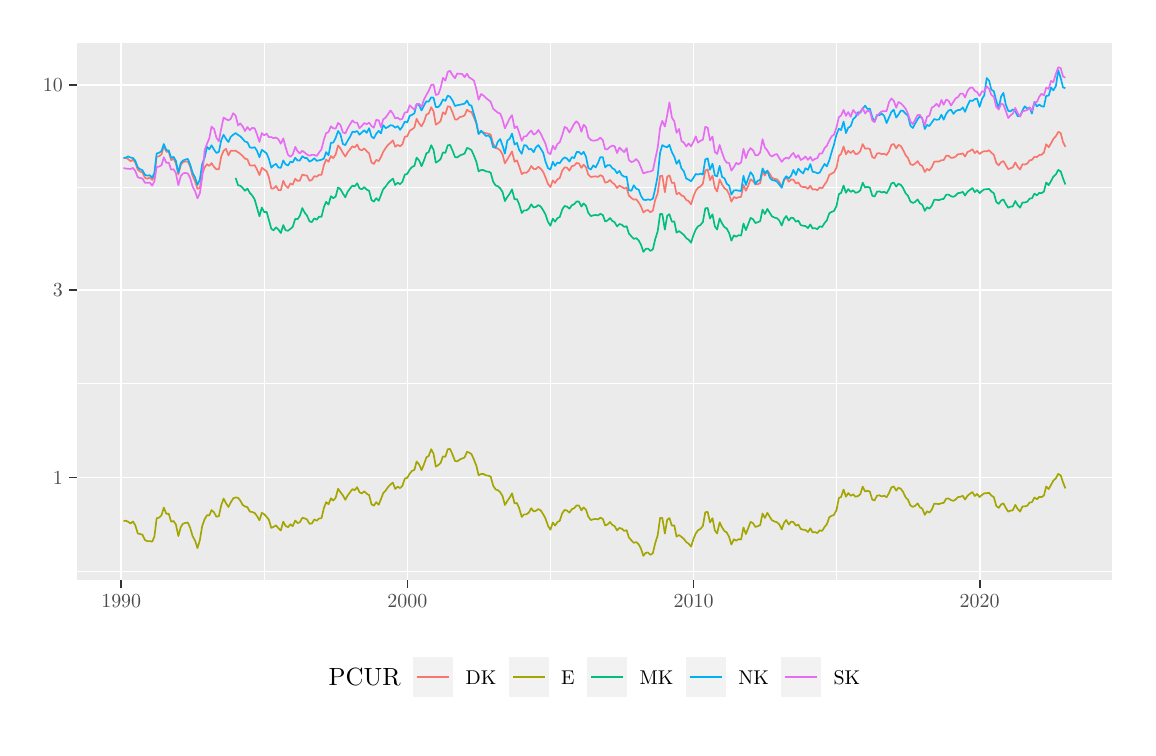
\begin{tikzpicture}[x=1pt,y=1pt]
\definecolor{fillColor}{RGB}{255,255,255}
\path[use as bounding box,fill=fillColor,fill opacity=0.00] (0,0) rectangle (397.48,252.94);
\begin{scope}
\path[clip] (  0.00,  0.00) rectangle (397.48,252.94);
\definecolor{drawColor}{RGB}{255,255,255}
\definecolor{fillColor}{RGB}{255,255,255}

\path[draw=drawColor,line width= 0.6pt,line join=round,line cap=round,fill=fillColor] (  0.00, -0.00) rectangle (397.48,252.94);
\end{scope}
\begin{scope}
\path[clip] ( 17.65, 53.26) rectangle (391.98,247.44);
\definecolor{fillColor}{gray}{0.92}

\path[fill=fillColor] ( 17.65, 53.26) rectangle (391.98,247.45);
\definecolor{drawColor}{RGB}{255,255,255}

\path[draw=drawColor,line width= 0.3pt,line join=round] ( 17.65, 56.61) --
	(391.98, 56.61);

\path[draw=drawColor,line width= 0.3pt,line join=round] ( 17.65,124.29) --
	(391.98,124.29);

\path[draw=drawColor,line width= 0.3pt,line join=round] ( 17.65,195.22) --
	(391.98,195.22);

\path[draw=drawColor,line width= 0.3pt,line join=round] ( 85.51, 53.26) --
	( 85.51,247.44);

\path[draw=drawColor,line width= 0.3pt,line join=round] (188.91, 53.26) --
	(188.91,247.44);

\path[draw=drawColor,line width= 0.3pt,line join=round] (292.31, 53.26) --
	(292.31,247.44);

\path[draw=drawColor,line width= 0.6pt,line join=round] ( 17.65, 90.45) --
	(391.98, 90.45);

\path[draw=drawColor,line width= 0.6pt,line join=round] ( 17.65,158.13) --
	(391.98,158.13);

\path[draw=drawColor,line width= 0.6pt,line join=round] ( 17.65,232.31) --
	(391.98,232.31);

\path[draw=drawColor,line width= 0.6pt,line join=round] ( 33.81, 53.26) --
	( 33.81,247.44);

\path[draw=drawColor,line width= 0.6pt,line join=round] (137.20, 53.26) --
	(137.20,247.44);

\path[draw=drawColor,line width= 0.6pt,line join=round] (240.61, 53.26) --
	(240.61,247.44);

\path[draw=drawColor,line width= 0.6pt,line join=round] (344.00, 53.26) --
	(344.00,247.44);
\definecolor{drawColor}{RGB}{248,118,109}

\path[draw=drawColor,line width= 0.6pt,line join=round] ( 34.66,205.85) --
	( 35.46,205.87) --
	( 36.31,205.44) --
	( 37.18,204.67) --
	( 38.06,205.27) --
	( 38.88,204.21) --
	( 39.79,201.61) --
	( 40.67,200.92) --
	( 41.46,200.62) --
	( 42.39,198.71) --
	( 43.24,198.33) --
	( 44.12,198.81) --
	( 45.00,197.88) --
	( 45.79,199.39) --
	( 46.61,206.40) --
	( 47.52,206.46) --
	( 48.39,207.18) --
	( 49.19,210.23) --
	( 50.12,208.10) --
	( 50.97,208.04) --
	( 51.85,205.07) --
	( 52.72,205.64) --
	( 53.55,203.93) --
	( 54.45,199.88) --
	( 55.33,203.30) --
	( 56.12,204.36) --
	( 57.03,204.58) --
	( 57.88,204.59) --
	( 58.70,202.75) --
	( 59.60,199.35) --
	( 60.48,197.40) --
	( 61.36,194.69) --
	( 62.21,195.07) --
	( 63.06,200.03) --
	( 63.94,202.42) --
	( 64.81,203.60) --
	( 65.63,202.99) --
	( 66.43,204.01) --
	( 67.36,202.60) --
	( 68.21,201.77) --
	( 69.09,201.80) --
	( 69.94,206.38) --
	( 70.79,208.47) --
	( 71.69,209.19) --
	( 72.54,206.76) --
	( 73.36,208.48) --
	( 74.27,208.42) --
	( 75.15,208.50) --
	( 76.02,207.88) --
	( 76.82,207.35) --
	( 77.69,206.56) --
	( 78.51,205.61) --
	( 79.42,205.38) --
	( 80.27,203.19) --
	( 81.09,203.11) --
	( 82.03,203.23) --
	( 82.87,201.69) --
	( 83.75,199.66) --
	( 84.60,202.31) --
	( 85.45,201.69) --
	( 86.36,201.04) --
	( 87.15,198.92) --
	( 88.03,194.84) --
	( 88.82,194.83) --
	( 89.75,195.74) --
	( 90.60,194.26) --
	( 91.48,194.21) --
	( 92.36,197.62) --
	( 93.18,195.88) --
	( 94.08,195.02) --
	( 94.93,196.64) --
	( 95.76,196.20) --
	( 96.69,198.36) --
	( 97.51,197.57) --
	( 98.33,197.66) --
	( 99.24,199.86) --
	(100.11,199.59) --
	(100.91,199.51) --
	(101.84,197.58) --
	(102.69,197.93) --
	(103.57,199.30) --
	(104.45,199.08) --
	(105.27,199.76) --
	(106.17,199.74) --
	(107.05,203.35) --
	(107.84,205.27) --
	(108.72,204.49) --
	(109.57,206.56) --
	(110.42,205.78) --
	(111.30,207.13) --
	(112.17,210.41) --
	(113.00,209.31) --
	(113.90,207.69) --
	(114.78,206.35) --
	(115.57,207.80) --
	(116.51,209.01) --
	(117.36,210.11) --
	(118.15,209.63) --
	(119.05,210.71) --
	(119.90,208.94) --
	(120.72,208.60) --
	(121.63,209.31) --
	(122.51,208.27) --
	(123.38,207.51) --
	(124.23,204.23) --
	(125.08,203.69) --
	(125.96,205.17) --
	(126.84,204.72) --
	(127.66,206.18) --
	(128.45,208.03) --
	(129.39,209.50) --
	(130.24,210.62) --
	(131.11,211.32) --
	(131.96,212.21) --
	(132.81,209.91) --
	(133.72,210.56) --
	(134.57,210.10) --
	(135.39,210.76) --
	(136.29,213.58) --
	(137.17,213.69) --
	(138.05,215.71) --
	(138.87,216.19) --
	(139.75,216.89) --
	(140.54,220.01) --
	(141.47,218.25) --
	(142.32,217.26) --
	(143.20,218.95) --
	(144.08,221.55) --
	(144.90,221.89) --
	(145.81,224.19) --
	(146.66,222.70) --
	(147.48,217.90) --
	(148.41,218.47) --
	(149.20,219.18) --
	(150.05,222.36) --
	(150.93,221.65) --
	(151.81,224.54) --
	(152.63,224.33) --
	(153.53,222.30) --
	(154.41,219.78) --
	(155.20,219.76) --
	(156.14,220.62) --
	(156.99,220.84) --
	(157.87,221.18) --
	(158.74,223.30) --
	(159.54,222.67) --
	(160.36,222.49) --
	(161.26,220.50) --
	(162.14,218.35) --
	(162.93,214.52) --
	(163.87,215.40) --
	(164.72,215.09) --
	(165.59,214.81) --
	(166.47,214.63) --
	(167.29,214.32) --
	(168.20,210.96) --
	(169.08,209.47) --
	(169.87,209.25) --
	(170.75,208.58) --
	(171.60,207.13) --
	(172.44,203.91) --
	(173.32,205.32) --
	(174.20,206.81) --
	(175.02,208.20) --
	(175.93,204.48) --
	(176.80,204.97) --
	(177.60,202.89) --
	(178.53,200.01) --
	(179.38,200.58) --
	(180.17,200.49) --
	(181.11,201.31) --
	(181.96,202.97) --
	(182.83,201.89) --
	(183.68,201.84) --
	(184.53,202.72) --
	(185.44,201.88) --
	(186.29,200.82) --
	(187.11,198.84) --
	(188.02,196.46) --
	(188.89,195.33) --
	(189.77,197.78) --
	(190.56,196.83) --
	(191.44,198.18) --
	(192.26,198.57) --
	(193.17,201.30) --
	(194.02,202.42) --
	(194.84,202.39) --
	(195.77,201.26) --
	(196.62,202.89) --
	(197.50,203.11) --
	(198.35,204.06) --
	(199.20,203.85) --
	(200.10,202.26) --
	(200.90,203.45) --
	(201.77,202.43) --
	(202.57,199.83) --
	(203.50,198.98) --
	(204.35,199.10) --
	(205.23,199.23) --
	(206.10,199.00) --
	(206.93,199.63) --
	(207.83,199.17) --
	(208.68,196.91) --
	(209.50,197.13) --
	(210.44,197.90) --
	(211.23,196.92) --
	(212.08,196.34) --
	(212.96,195.00) --
	(213.83,195.88) --
	(214.65,195.41) --
	(215.56,194.82) --
	(216.44,195.11) --
	(217.23,192.30) --
	(218.16,191.39) --
	(219.01,190.78) --
	(219.89,190.94) --
	(220.77,189.78) --
	(221.59,188.44) --
	(222.47,186.15) --
	(223.32,186.81) --
	(224.17,187.04) --
	(225.04,186.23) --
	(225.92,186.86) --
	(226.74,190.64) --
	(227.65,193.08) --
	(228.53,199.31) --
	(229.32,199.46) --
	(230.25,193.47) --
	(231.10,199.09) --
	(231.89,199.59) --
	(232.80,196.82) --
	(233.65,196.92) --
	(234.47,192.75) --
	(235.38,193.26) --
	(236.25,192.32) --
	(237.13,191.95) --
	(237.98,190.66) --
	(238.83,190.28) --
	(239.71,189.09) --
	(240.59,191.99) --
	(241.41,194.00) --
	(242.20,195.04) --
	(243.13,195.59) --
	(243.98,196.55) --
	(244.86,201.31) --
	(245.71,201.73) --
	(246.56,197.81) --
	(247.46,199.47) --
	(248.31,195.10) --
	(249.13,193.73) --
	(250.04,198.11) --
	(250.92,196.27) --
	(251.80,194.86) --
	(252.59,194.37) --
	(253.47,192.76) --
	(254.29,190.04) --
	(255.19,191.77) --
	(256.04,191.33) --
	(256.86,191.67) --
	(257.80,191.79) --
	(258.65,196.10) --
	(259.52,194.00) --
	(260.37,195.84) --
	(261.22,198.15) --
	(262.13,197.50) --
	(262.95,196.35) --
	(263.80,196.32) --
	(264.68,196.79) --
	(265.55,200.96) --
	(266.38,199.51) --
	(267.28,201.32) --
	(268.16,200.06) --
	(268.95,198.72) --
	(269.89,198.27) --
	(270.73,198.16) --
	(271.61,197.17) --
	(272.49,195.41) --
	(273.28,197.80) --
	(274.10,198.92) --
	(275.01,197.27) --
	(275.89,198.07) --
	(276.68,198.03) --
	(277.61,196.63) --
	(278.46,197.04) --
	(279.34,195.62) --
	(280.22,195.36) --
	(281.04,195.35) --
	(281.95,194.67) --
	(282.82,195.83) --
	(283.62,194.42) --
	(284.49,194.60) --
	(285.34,194.15) --
	(286.19,195.19) --
	(287.07,194.86) --
	(287.95,196.24) --
	(288.77,197.37) --
	(289.67,199.73) --
	(290.55,200.24) --
	(291.34,200.62) --
	(292.28,202.41) --
	(293.13,206.57) --
	(293.92,207.34) --
	(294.83,210.00) --
	(295.68,207.19) --
	(296.50,208.44) --
	(297.40,207.62) --
	(298.28,208.49) --
	(299.16,207.24) --
	(300.01,207.41) --
	(300.86,208.34) --
	(301.73,210.88) --
	(302.61,209.20) --
	(303.43,209.34) --
	(304.31,209.09) --
	(305.19,206.22) --
	(306.01,205.77) --
	(306.91,207.47) --
	(307.76,207.60) --
	(308.58,207.24) --
	(309.52,207.36) --
	(310.37,206.92) --
	(311.25,208.30) --
	(312.09,210.56) --
	(312.94,210.90) --
	(313.85,209.33) --
	(314.64,210.58) --
	(315.52,210.17) --
	(316.31,208.79) --
	(317.25,206.85) --
	(318.10,205.84) --
	(318.97,203.64) --
	(319.85,203.30) --
	(320.67,203.83) --
	(321.58,204.71) --
	(322.43,203.37) --
	(323.25,202.91) --
	(324.18,200.79) --
	(324.98,201.92) --
	(325.82,201.33) --
	(326.70,202.54) --
	(327.58,204.48) --
	(328.40,204.59) --
	(329.31,204.56) --
	(330.18,205.06) --
	(330.98,205.07) --
	(331.91,206.67) --
	(332.76,206.65) --
	(333.64,205.87) --
	(334.52,205.97) --
	(335.31,206.35) --
	(336.13,207.22) --
	(337.04,207.24) --
	(337.91,207.51) --
	(338.71,206.37) --
	(339.64,208.02) --
	(340.49,208.40) --
	(341.37,209.00) --
	(342.24,207.63) --
	(343.07,208.38) --
	(343.97,207.29) --
	(344.85,207.97) --
	(345.64,208.33) --
	(346.55,208.24) --
	(347.40,208.66) --
	(348.22,207.74) --
	(349.12,207.02) --
	(350.00,204.07) --
	(350.88,203.21) --
	(351.73,204.35) --
	(352.58,204.73) --
	(353.45,203.25) --
	(354.33,201.78) --
	(355.15,202.14) --
	(355.95,202.45) --
	(356.88,204.23) --
	(357.73,202.72) --
	(358.61,201.67) --
	(359.46,203.57) --
	(360.31,203.51) --
	(361.21,203.82) --
	(362.06,205.04) --
	(362.88,205.14) --
	(363.79,206.32) --
	(364.67,206.15) --
	(365.54,206.93) --
	(366.34,206.99) --
	(367.21,207.83) --
	(368.03,210.82) --
	(368.94,209.72) --
	(369.79,211.15) --
	(370.61,212.74) --
	(371.54,213.73) --
	(372.39,215.27) --
	(373.27,214.86) --
	(374.12,211.61) --
	(374.97,209.87);
\definecolor{drawColor}{RGB}{163,165,0}

\path[draw=drawColor,line width= 0.6pt,line join=round] ( 34.66, 74.67) --
	( 35.46, 74.78) --
	( 36.31, 74.37) --
	( 37.18, 73.79) --
	( 38.06, 74.49) --
	( 38.88, 73.14) --
	( 39.79, 70.15) --
	( 40.67, 69.95) --
	( 41.46, 69.75) --
	( 42.39, 67.77) --
	( 43.24, 67.41) --
	( 44.12, 67.40) --
	( 45.00, 67.22) --
	( 45.79, 69.01) --
	( 46.61, 75.66) --
	( 47.52, 75.90) --
	( 48.39, 76.82) --
	( 49.19, 79.52) --
	( 50.12, 77.25) --
	( 50.97, 77.33) --
	( 51.85, 74.42) --
	( 52.72, 74.67) --
	( 53.55, 73.44) --
	( 54.45, 69.24) --
	( 55.33, 72.52) --
	( 56.12, 73.68) --
	( 57.03, 74.01) --
	( 57.88, 74.11) --
	( 58.70, 72.27) --
	( 59.60, 69.18) --
	( 60.48, 67.56) --
	( 61.36, 64.88) --
	( 62.21, 67.70) --
	( 63.06, 72.85) --
	( 63.94, 75.31) --
	( 64.81, 76.78) --
	( 65.63, 76.68) --
	( 66.43, 78.64) --
	( 67.36, 77.77) --
	( 68.21, 76.20) --
	( 69.09, 76.43) --
	( 69.94, 80.33) --
	( 70.79, 82.79) --
	( 71.69, 81.05) --
	( 72.54, 79.73) --
	( 73.36, 81.35) --
	( 74.27, 82.85) --
	( 75.15, 83.19) --
	( 76.02, 83.06) --
	( 76.82, 82.06) --
	( 77.69, 80.48) --
	( 78.51, 79.96) --
	( 79.42, 79.65) --
	( 80.27, 78.07) --
	( 81.09, 77.93) --
	( 82.03, 77.57) --
	( 82.87, 76.48) --
	( 83.75, 74.93) --
	( 84.60, 77.62) --
	( 85.45, 77.14) --
	( 86.36, 76.16) --
	( 87.15, 75.14) --
	( 88.03, 72.17) --
	( 88.82, 72.55) --
	( 89.75, 73.09) --
	( 90.60, 72.04) --
	( 91.48, 71.26) --
	( 92.36, 74.46) --
	( 93.18, 72.93) --
	( 94.08, 72.43) --
	( 94.93, 73.50) --
	( 95.76, 72.81) --
	( 96.69, 74.84) --
	( 97.51, 73.94) --
	( 98.33, 74.20) --
	( 99.24, 75.83) --
	(100.11, 75.62) --
	(100.91, 75.27) --
	(101.84, 73.68) --
	(102.69, 73.79) --
	(103.57, 75.25) --
	(104.45, 74.77) --
	(105.27, 75.59) --
	(106.17, 75.67) --
	(107.05, 79.38) --
	(107.84, 81.49) --
	(108.72, 80.75) --
	(109.57, 82.88) --
	(110.42, 82.05) --
	(111.30, 83.09) --
	(112.17, 86.33) --
	(113.00, 85.13) --
	(113.90, 83.93) --
	(114.78, 82.34) --
	(115.57, 83.84) --
	(116.51, 85.10) --
	(117.36, 86.19) --
	(118.15, 85.78) --
	(119.05, 86.91) --
	(119.90, 85.09) --
	(120.72, 84.66) --
	(121.63, 85.39) --
	(122.51, 84.52) --
	(123.38, 84.03) --
	(124.23, 80.74) --
	(125.08, 80.21) --
	(125.96, 81.48) --
	(126.84, 80.55) --
	(127.66, 82.61) --
	(128.45, 84.70) --
	(129.39, 85.73) --
	(130.24, 86.97) --
	(131.11, 87.86) --
	(131.96, 88.55) --
	(132.81, 86.26) --
	(133.72, 87.07) --
	(134.57, 86.57) --
	(135.39, 87.38) --
	(136.29, 90.02) --
	(137.17, 90.30) --
	(138.05, 91.79) --
	(138.87, 92.78) --
	(139.75, 93.16) --
	(140.54, 96.17) --
	(141.47, 95.09) --
	(142.32, 93.05) --
	(143.20, 95.14) --
	(144.08, 97.69) --
	(144.90, 98.15) --
	(145.81,100.63) --
	(146.66, 98.99) --
	(147.48, 94.33) --
	(148.41, 94.92) --
	(149.20, 95.61) --
	(150.05, 98.04) --
	(150.93, 97.86) --
	(151.81,100.63) --
	(152.63,100.71) --
	(153.53, 98.67) --
	(154.41, 96.37) --
	(155.20, 96.21) --
	(156.14, 96.89) --
	(156.99, 97.25) --
	(157.87, 97.60) --
	(158.74, 99.68) --
	(159.54, 99.38) --
	(160.36, 98.86) --
	(161.26, 96.86) --
	(162.14, 94.63) --
	(162.93, 91.22) --
	(163.87, 91.67) --
	(164.72, 91.65) --
	(165.59, 91.17) --
	(166.47, 91.05) --
	(167.29, 90.77) --
	(168.20, 87.48) --
	(169.08, 86.08) --
	(169.87, 85.83) --
	(170.75, 85.07) --
	(171.60, 83.69) --
	(172.44, 80.45) --
	(173.32, 81.93) --
	(174.20, 83.16) --
	(175.02, 84.69) --
	(175.93, 81.06) --
	(176.80, 81.17) --
	(177.60, 79.28) --
	(178.53, 76.14) --
	(179.38, 77.08) --
	(180.17, 77.07) --
	(181.11, 77.75) --
	(181.96, 79.28) --
	(182.83, 78.14) --
	(183.68, 78.37) --
	(184.53, 79.01) --
	(185.44, 78.43) --
	(186.29, 77.10) --
	(187.11, 75.62) --
	(188.02, 72.92) --
	(188.89, 71.54) --
	(189.77, 74.12) --
	(190.56, 73.00) --
	(191.44, 74.30) --
	(192.26, 74.71) --
	(193.17, 77.46) --
	(194.02, 78.67) --
	(194.84, 78.47) --
	(195.77, 77.70) --
	(196.62, 78.93) --
	(197.50, 79.33) --
	(198.35, 80.31) --
	(199.20, 80.27) --
	(200.10, 78.49) --
	(200.90, 79.61) --
	(201.77, 78.70) --
	(202.57, 76.23) --
	(203.50, 75.03) --
	(204.35, 75.30) --
	(205.23, 75.42) --
	(206.10, 75.24) --
	(206.93, 75.88) --
	(207.83, 75.41) --
	(208.68, 73.08) --
	(209.50, 73.41) --
	(210.44, 74.31) --
	(211.23, 73.30) --
	(212.08, 72.83) --
	(212.96, 71.29) --
	(213.83, 72.16) --
	(214.65, 71.93) --
	(215.56, 71.10) --
	(216.44, 71.36) --
	(217.23, 68.75) --
	(218.16, 67.69) --
	(219.01, 66.80) --
	(219.89, 67.05) --
	(220.77, 66.27) --
	(221.59, 64.73) --
	(222.47, 62.09) --
	(223.32, 63.17) --
	(224.17, 63.29) --
	(225.04, 62.44) --
	(225.92, 63.04) --
	(226.74, 66.62) --
	(227.65, 69.51) --
	(228.53, 75.82) --
	(229.32, 75.78) --
	(230.25, 70.16) --
	(231.10, 75.17) --
	(231.89, 75.72) --
	(232.80, 72.98) --
	(233.65, 73.11) --
	(234.47, 69.04) --
	(235.38, 69.60) --
	(236.25, 68.94) --
	(237.13, 68.19) --
	(237.98, 67.06) --
	(238.83, 66.48) --
	(239.71, 65.41) --
	(240.59, 68.21) --
	(241.41, 70.16) --
	(242.20, 71.29) --
	(243.13, 71.82) --
	(243.98, 72.89) --
	(244.86, 77.84) --
	(245.71, 77.95) --
	(246.56, 74.15) --
	(247.46, 75.68) --
	(248.31, 71.27) --
	(249.13, 70.16) --
	(250.04, 74.20) --
	(250.92, 72.35) --
	(251.80, 71.01) --
	(252.59, 70.55) --
	(253.47, 68.88) --
	(254.29, 66.15) --
	(255.19, 68.09) --
	(256.04, 67.56) --
	(256.86, 68.11) --
	(257.80, 67.99) --
	(258.65, 72.34) --
	(259.52, 69.95) --
	(260.37, 72.13) --
	(261.22, 74.37) --
	(262.13, 73.86) --
	(262.95, 72.52) --
	(263.80, 72.80) --
	(264.68, 73.18) --
	(265.55, 77.37) --
	(266.38, 75.77) --
	(267.28, 77.62) --
	(268.16, 76.19) --
	(268.95, 74.93) --
	(269.89, 74.48) --
	(270.73, 74.26) --
	(271.61, 73.42) --
	(272.49, 71.62) --
	(273.28, 73.94) --
	(274.10, 75.04) --
	(275.01, 73.42) --
	(275.89, 74.47) --
	(276.68, 74.29) --
	(277.61, 72.98) --
	(278.46, 73.41) --
	(279.34, 71.79) --
	(280.22, 71.53) --
	(281.04, 71.43) --
	(281.95, 70.70) --
	(282.82, 72.03) --
	(283.62, 70.55) --
	(284.49, 70.68) --
	(285.34, 70.31) --
	(286.19, 71.30) --
	(287.07, 71.09) --
	(287.95, 72.51) --
	(288.77, 73.47) --
	(289.67, 76.05) --
	(290.55, 76.56) --
	(291.34, 76.87) --
	(292.28, 78.70) --
	(293.13, 83.00) --
	(293.92, 83.37) --
	(294.83, 86.05) --
	(295.68, 83.44) --
	(296.50, 84.78) --
	(297.40, 83.79) --
	(298.28, 84.30) --
	(299.16, 83.44) --
	(300.01, 83.67) --
	(300.86, 84.32) --
	(301.73, 87.08) --
	(302.61, 85.35) --
	(303.43, 85.59) --
	(304.31, 85.33) --
	(305.19, 82.40) --
	(306.01, 82.09) --
	(306.91, 83.84) --
	(307.76, 83.97) --
	(308.58, 83.56) --
	(309.52, 83.81) --
	(310.37, 83.26) --
	(311.25, 84.79) --
	(312.09, 86.81) --
	(312.94, 87.16) --
	(313.85, 85.67) --
	(314.64, 86.71) --
	(315.52, 86.31) --
	(316.31, 85.20) --
	(317.25, 83.22) --
	(318.10, 82.35) --
	(318.97, 80.30) --
	(319.85, 79.79) --
	(320.67, 80.14) --
	(321.58, 81.04) --
	(322.43, 79.61) --
	(323.25, 79.17) --
	(324.18, 76.91) --
	(324.98, 78.21) --
	(325.82, 77.70) --
	(326.70, 78.80) --
	(327.58, 80.92) --
	(328.40, 80.90) --
	(329.31, 80.77) --
	(330.18, 81.12) --
	(330.98, 81.22) --
	(331.91, 82.75) --
	(332.76, 82.80) --
	(333.64, 82.21) --
	(334.52, 81.97) --
	(335.31, 82.45) --
	(336.13, 83.31) --
	(337.04, 83.43) --
	(337.91, 83.78) --
	(338.71, 82.44) --
	(339.64, 83.83) --
	(340.49, 84.51) --
	(341.37, 85.13) --
	(342.24, 83.71) --
	(343.07, 84.43) --
	(343.97, 83.33) --
	(344.85, 84.12) --
	(345.64, 84.66) --
	(346.55, 84.73) --
	(347.40, 84.84) --
	(348.22, 83.89) --
	(349.12, 83.29) --
	(350.00, 80.12) --
	(350.88, 79.42) --
	(351.73, 80.64) --
	(352.58, 81.05) --
	(353.45, 79.41) --
	(354.33, 78.02) --
	(355.15, 78.45) --
	(355.95, 78.51) --
	(356.88, 80.50) --
	(357.73, 79.02) --
	(358.61, 78.06) --
	(359.46, 79.94) --
	(360.31, 79.95) --
	(361.21, 80.23) --
	(362.06, 81.36) --
	(362.88, 81.45) --
	(363.79, 83.16) --
	(364.67, 82.53) --
	(365.54, 83.41) --
	(366.34, 83.29) --
	(367.21, 83.87) --
	(368.03, 87.15) --
	(368.94, 86.21) --
	(369.79, 87.71) --
	(370.61, 89.25) --
	(371.54, 90.11) --
	(372.39, 91.71) --
	(373.27, 91.17) --
	(374.12, 88.65) --
	(374.97, 86.44);
\definecolor{drawColor}{RGB}{0,191,125}

\path[draw=drawColor,line width= 0.6pt,line join=round] ( 75.15,198.65) --
	( 76.02,196.01) --
	( 76.82,195.83) --
	( 77.69,195.04) --
	( 78.51,194.00) --
	( 79.42,194.80) --
	( 80.27,193.23) --
	( 81.09,192.37) --
	( 82.03,190.84) --
	( 82.87,187.89) --
	( 83.75,184.75) --
	( 84.60,187.94) --
	( 85.45,186.31) --
	( 86.36,186.36) --
	( 87.15,183.47) --
	( 88.03,180.29) --
	( 88.82,179.69) --
	( 89.75,180.77) --
	( 90.60,179.99) --
	( 91.48,178.71) --
	( 92.36,181.61) --
	( 93.18,179.74) --
	( 94.08,179.55) --
	( 94.93,180.23) --
	( 95.76,180.91) --
	( 96.69,183.84) --
	( 97.51,183.73) --
	( 98.33,184.92) --
	( 99.24,187.75) --
	(100.11,186.05) --
	(100.91,185.08) --
	(101.84,182.98) --
	(102.69,182.68) --
	(103.57,184.03) --
	(104.45,183.54) --
	(105.27,184.60) --
	(106.17,184.59) --
	(107.05,188.14) --
	(107.84,190.03) --
	(108.72,189.02) --
	(109.57,192.06) --
	(110.42,191.30) --
	(111.30,191.95) --
	(112.17,195.20) --
	(113.00,194.57) --
	(113.90,193.03) --
	(114.78,191.63) --
	(115.57,193.55) --
	(116.51,194.86) --
	(117.36,195.87) --
	(118.15,195.59) --
	(119.05,196.72) --
	(119.90,194.89) --
	(120.72,194.55) --
	(121.63,195.32) --
	(122.51,194.42) --
	(123.38,193.96) --
	(124.23,190.69) --
	(125.08,190.08) --
	(125.96,191.33) --
	(126.84,190.38) --
	(127.66,192.44) --
	(128.45,194.53) --
	(129.39,195.56) --
	(130.24,196.81) --
	(131.11,197.69) --
	(131.96,198.38) --
	(132.81,196.09) --
	(133.72,196.90) --
	(134.57,196.40) --
	(135.39,197.21) --
	(136.29,199.85) --
	(137.17,200.13) --
	(138.05,201.63) --
	(138.87,202.61) --
	(139.75,202.99) --
	(140.54,206.00) --
	(141.47,204.92) --
	(142.32,202.88) --
	(143.20,204.97) --
	(144.08,207.52) --
	(144.90,207.98) --
	(145.81,210.46) --
	(146.66,208.82) --
	(147.48,204.16) --
	(148.41,204.75) --
	(149.20,205.44) --
	(150.05,207.87) --
	(150.93,207.69) --
	(151.81,210.46) --
	(152.63,210.54) --
	(153.53,208.51) --
	(154.41,206.20) --
	(155.20,206.04) --
	(156.14,206.72) --
	(156.99,207.09) --
	(157.87,207.43) --
	(158.74,209.50) --
	(159.54,209.21) --
	(160.36,208.69) --
	(161.26,206.69) --
	(162.14,204.47) --
	(162.93,201.04) --
	(163.87,201.50) --
	(164.72,201.48) --
	(165.59,201.00) --
	(166.47,200.88) --
	(167.29,200.60) --
	(168.20,197.31) --
	(169.08,195.91) --
	(169.87,195.66) --
	(170.75,194.90) --
	(171.60,193.51) --
	(172.44,190.28) --
	(173.32,191.75) --
	(174.20,192.99) --
	(175.02,194.52) --
	(175.93,190.89) --
	(176.80,191.00) --
	(177.60,189.11) --
	(178.53,185.97) --
	(179.38,186.91) --
	(180.17,186.90) --
	(181.11,187.58) --
	(181.96,189.11) --
	(182.83,187.97) --
	(183.68,188.19) --
	(184.53,188.84) --
	(185.44,188.26) --
	(186.29,186.92) --
	(187.11,185.45) --
	(188.02,182.75) --
	(188.89,181.37) --
	(189.77,183.94) --
	(190.56,182.83) --
	(191.44,184.13) --
	(192.26,184.54) --
	(193.17,187.28) --
	(194.02,188.50) --
	(194.84,188.30) --
	(195.77,187.53) --
	(196.62,188.75) --
	(197.50,189.16) --
	(198.35,190.13) --
	(199.20,190.10) --
	(200.10,188.31) --
	(200.90,189.44) --
	(201.77,188.52) --
	(202.57,186.05) --
	(203.50,184.85) --
	(204.35,185.13) --
	(205.23,185.25) --
	(206.10,185.07) --
	(206.93,185.71) --
	(207.83,185.24) --
	(208.68,182.91) --
	(209.50,183.23) --
	(210.44,184.14) --
	(211.23,183.13) --
	(212.08,182.65) --
	(212.96,181.12) --
	(213.83,181.99) --
	(214.65,181.76) --
	(215.56,180.93) --
	(216.44,181.19) --
	(217.23,178.58) --
	(218.16,177.52) --
	(219.01,176.63) --
	(219.89,176.87) --
	(220.77,176.10) --
	(221.59,174.56) --
	(222.47,171.92) --
	(223.32,173.00) --
	(224.17,173.11) --
	(225.04,172.27) --
	(225.92,172.87) --
	(226.74,176.45) --
	(227.65,179.34) --
	(228.53,185.64) --
	(229.32,185.60) --
	(230.25,179.99) --
	(231.10,184.99) --
	(231.89,185.55) --
	(232.80,182.81) --
	(233.65,182.93) --
	(234.47,178.87) --
	(235.38,179.43) --
	(236.25,178.77) --
	(237.13,178.02) --
	(237.98,176.89) --
	(238.83,176.31) --
	(239.71,175.24) --
	(240.59,178.04) --
	(241.41,179.99) --
	(242.20,181.12) --
	(243.13,181.65) --
	(243.98,182.72) --
	(244.86,187.67) --
	(245.71,187.78) --
	(246.56,183.98) --
	(247.46,185.50) --
	(248.31,181.10) --
	(249.13,179.99) --
	(250.04,184.03) --
	(250.92,182.17) --
	(251.80,180.84) --
	(252.59,180.38) --
	(253.47,178.71) --
	(254.29,175.97) --
	(255.19,177.91) --
	(256.04,177.39) --
	(256.86,177.94) --
	(257.80,177.82) --
	(258.65,182.17) --
	(259.52,179.78) --
	(260.37,181.96) --
	(261.22,184.20) --
	(262.13,183.68) --
	(262.95,182.35) --
	(263.80,182.63) --
	(264.68,183.01) --
	(265.55,187.20) --
	(266.38,185.60) --
	(267.28,187.44) --
	(268.16,186.01) --
	(268.95,184.76) --
	(269.89,184.31) --
	(270.73,184.08) --
	(271.61,183.25) --
	(272.49,181.45) --
	(273.28,183.76) --
	(274.10,184.87) --
	(275.01,183.25) --
	(275.89,184.30) --
	(276.68,184.12) --
	(277.61,182.81) --
	(278.46,183.24) --
	(279.34,181.62) --
	(280.22,181.35) --
	(281.04,181.26) --
	(281.95,180.52) --
	(282.82,181.85) --
	(283.62,180.38) --
	(284.49,180.51) --
	(285.34,180.14) --
	(286.19,181.13) --
	(287.07,180.92) --
	(287.95,182.34) --
	(288.77,183.30) --
	(289.67,185.88) --
	(290.55,186.39) --
	(291.34,186.69) --
	(292.28,188.53) --
	(293.13,192.83) --
	(293.92,193.20) --
	(294.83,195.88) --
	(295.68,193.26) --
	(296.50,194.61) --
	(297.40,193.61) --
	(298.28,194.13) --
	(299.16,193.27) --
	(300.01,193.50) --
	(300.86,194.14) --
	(301.73,196.91) --
	(302.61,195.18) --
	(303.43,195.42) --
	(304.31,195.16) --
	(305.19,192.23) --
	(306.01,191.91) --
	(306.91,193.67) --
	(307.76,193.79) --
	(308.58,193.39) --
	(309.52,193.64) --
	(310.37,193.09) --
	(311.25,194.62) --
	(312.09,196.64) --
	(312.94,196.99) --
	(313.85,195.49) --
	(314.64,196.53) --
	(315.52,196.13) --
	(316.31,195.03) --
	(317.25,193.05) --
	(318.10,192.17) --
	(318.97,190.13) --
	(319.85,189.62) --
	(320.67,189.96) --
	(321.58,190.87) --
	(322.43,189.44) --
	(323.25,189.00) --
	(324.18,186.74) --
	(324.98,188.04) --
	(325.82,187.53) --
	(326.70,188.62) --
	(327.58,190.75) --
	(328.40,190.73) --
	(329.31,190.60) --
	(330.18,190.95) --
	(330.98,191.05) --
	(331.91,192.58) --
	(332.76,192.62) --
	(333.64,192.03) --
	(334.52,191.80) --
	(335.31,192.27) --
	(336.13,193.14) --
	(337.04,193.26) --
	(337.91,193.61) --
	(338.71,192.27) --
	(339.64,193.66) --
	(340.49,194.33) --
	(341.37,194.96) --
	(342.24,193.53) --
	(343.07,194.26) --
	(343.97,193.16) --
	(344.85,193.95) --
	(345.64,194.49) --
	(346.55,194.56) --
	(347.40,194.67) --
	(348.22,193.72) --
	(349.12,193.12) --
	(350.00,189.95) --
	(350.88,189.25) --
	(351.73,190.46) --
	(352.58,190.87) --
	(353.45,189.24) --
	(354.33,187.85) --
	(355.15,188.28) --
	(355.95,188.34) --
	(356.88,190.32) --
	(357.73,188.85) --
	(358.61,187.89) --
	(359.46,189.77) --
	(360.31,189.78) --
	(361.21,190.06) --
	(362.06,191.19) --
	(362.88,191.28) --
	(363.79,192.99) --
	(364.67,192.35) --
	(365.54,193.24) --
	(366.34,193.12) --
	(367.21,193.70) --
	(368.03,196.98) --
	(368.94,196.04) --
	(369.79,197.54) --
	(370.61,199.08) --
	(371.54,199.93) --
	(372.39,201.54) --
	(373.27,201.00) --
	(374.12,198.48) --
	(374.97,196.27);
\definecolor{drawColor}{RGB}{0,176,246}

\path[draw=drawColor,line width= 0.6pt,line join=round] ( 34.66,205.79) --
	( 35.46,205.98) --
	( 36.31,206.40) --
	( 37.18,206.00) --
	( 38.06,205.81) --
	( 38.88,204.87) --
	( 39.79,202.41) --
	( 40.67,201.75) --
	( 41.46,201.45) --
	( 42.39,199.75) --
	( 43.24,199.46) --
	( 44.12,199.62) --
	( 45.00,198.77) --
	( 45.79,200.45) --
	( 46.61,207.47) --
	( 47.52,207.75) --
	( 48.39,208.40) --
	( 49.19,210.89) --
	( 50.12,208.64) --
	( 50.97,208.59) --
	( 51.85,205.92) --
	( 52.72,206.25) --
	( 53.55,204.84) --
	( 54.45,200.55) --
	( 55.33,204.05) --
	( 56.12,204.93) --
	( 57.03,205.30) --
	( 57.88,205.51) --
	( 58.70,203.51) --
	( 59.60,200.51) --
	( 60.48,198.83) --
	( 61.36,196.13) --
	( 62.21,198.07) --
	( 63.06,203.70) --
	( 63.94,205.93) --
	( 64.81,209.89) --
	( 65.63,208.98) --
	( 66.43,210.45) --
	( 67.36,208.88) --
	( 68.21,207.66) --
	( 69.09,208.05) --
	( 69.94,212.23) --
	( 70.79,214.26) --
	( 71.69,212.73) --
	( 72.54,211.61) --
	( 73.36,213.49) --
	( 74.27,214.25) --
	( 75.15,214.86) --
	( 76.02,214.17) --
	( 76.82,213.67) --
	( 77.69,212.77) --
	( 78.51,211.82) --
	( 79.42,211.52) --
	( 80.27,209.68) --
	( 81.09,209.50) --
	( 82.03,209.74) --
	( 82.87,208.42) --
	( 83.75,206.11) --
	( 84.60,208.80) --
	( 85.45,208.21) --
	( 86.36,207.49) --
	( 87.15,205.53) --
	( 88.03,202.33) --
	( 88.82,203.18) --
	( 89.75,203.72) --
	( 90.60,202.42) --
	( 91.48,202.28) --
	( 92.36,204.97) --
	( 93.18,203.60) --
	( 94.08,203.11) --
	( 94.93,204.53) --
	( 95.76,204.27) --
	( 96.69,205.92) --
	( 97.51,204.93) --
	( 98.33,204.92) --
	( 99.24,206.47) --
	(100.11,205.85) --
	(100.91,205.82) --
	(101.84,204.51) --
	(102.69,204.96) --
	(103.57,205.76) --
	(104.45,204.79) --
	(105.27,205.02) --
	(106.17,205.21) --
	(107.05,205.64) --
	(107.84,207.98) --
	(108.72,206.85) --
	(109.57,211.34) --
	(110.42,211.40) --
	(111.30,213.14) --
	(112.17,215.61) --
	(113.00,214.44) --
	(113.90,210.93) --
	(114.78,210.48) --
	(115.57,212.03) --
	(116.51,213.54) --
	(117.36,215.36) --
	(118.15,215.23) --
	(119.05,215.59) --
	(119.90,214.26) --
	(120.72,215.05) --
	(121.63,215.88) --
	(122.51,214.92) --
	(123.38,216.63) --
	(124.23,213.61) --
	(125.08,212.94) --
	(125.96,214.62) --
	(126.84,215.66) --
	(127.66,214.73) --
	(128.45,217.71) --
	(129.39,216.63) --
	(130.24,217.07) --
	(131.11,217.71) --
	(131.96,217.55) --
	(132.81,216.81) --
	(133.72,217.36) --
	(134.57,216.04) --
	(135.39,217.17) --
	(136.29,219.02) --
	(137.17,218.69) --
	(138.05,221.08) --
	(138.87,221.43) --
	(139.75,222.02) --
	(140.54,225.31) --
	(141.47,224.87) --
	(142.32,223.02) --
	(143.20,224.83) --
	(144.08,226.33) --
	(144.90,226.21) --
	(145.81,227.77) --
	(146.66,227.59) --
	(147.48,224.23) --
	(148.41,224.30) --
	(149.20,225.20) --
	(150.05,227.00) --
	(150.93,226.49) --
	(151.81,228.41) --
	(152.63,227.97) --
	(153.53,226.61) --
	(154.41,224.64) --
	(155.20,224.91) --
	(156.14,225.07) --
	(156.99,225.28) --
	(157.87,225.45) --
	(158.74,226.61) --
	(159.54,225.00) --
	(160.36,224.78) --
	(161.26,221.66) --
	(162.14,218.59) --
	(162.93,214.52) --
	(163.87,215.71) --
	(164.72,214.71) --
	(165.59,213.79) --
	(166.47,214.03) --
	(167.29,213.12) --
	(168.20,209.71) --
	(169.08,209.63) --
	(169.87,211.70) --
	(170.75,212.69) --
	(171.60,210.32) --
	(172.44,207.41) --
	(173.32,212.14) --
	(174.20,212.83) --
	(175.02,214.68) --
	(175.93,210.71) --
	(176.80,211.30) --
	(177.60,208.71) --
	(178.53,207.37) --
	(179.38,210.49) --
	(180.17,210.38) --
	(181.11,208.98) --
	(181.96,209.12) --
	(182.83,207.95) --
	(183.68,209.73) --
	(184.53,210.50) --
	(185.44,209.12) --
	(186.29,207.73) --
	(187.11,204.54) --
	(188.02,202.18) --
	(188.89,201.65) --
	(189.77,204.47) --
	(190.56,203.00) --
	(191.44,204.21) --
	(192.26,203.96) --
	(193.17,205.34) --
	(194.02,206.06) --
	(194.84,205.67) --
	(195.77,204.56) --
	(196.62,206.18) --
	(197.50,205.80) --
	(198.35,208.00) --
	(199.20,208.05) --
	(200.10,207.16) --
	(200.90,208.07) --
	(201.77,206.27) --
	(202.57,202.26) --
	(203.50,201.69) --
	(204.35,203.15) --
	(205.23,202.45) --
	(206.10,204.07) --
	(206.93,206.17) --
	(207.83,206.11) --
	(208.68,202.47) --
	(209.50,203.22) --
	(210.44,203.27) --
	(211.23,202.20) --
	(212.08,201.69) --
	(212.96,200.35) --
	(213.83,201.17) --
	(214.65,199.69) --
	(215.56,199.10) --
	(216.44,199.08) --
	(217.23,194.23) --
	(218.16,193.99) --
	(219.01,195.99) --
	(219.89,194.76) --
	(220.77,194.44) --
	(221.59,192.19) --
	(222.47,190.80) --
	(223.32,190.64) --
	(224.17,190.88) --
	(225.04,190.68) --
	(225.92,191.16) --
	(226.74,194.64) --
	(227.65,199.40) --
	(228.53,207.79) --
	(229.32,210.52) --
	(230.25,209.95) --
	(231.10,209.74) --
	(231.89,210.61) --
	(232.80,207.93) --
	(233.65,206.33) --
	(234.47,203.74) --
	(235.38,205.09) --
	(236.25,202.06) --
	(237.13,201.01) --
	(237.98,198.43) --
	(238.83,198.02) --
	(239.71,197.44) --
	(240.59,198.70) --
	(241.41,200.08) --
	(242.20,199.86) --
	(243.13,200.21) --
	(243.98,199.86) --
	(244.86,205.34) --
	(245.71,205.74) --
	(246.56,201.60) --
	(247.46,203.78) --
	(248.31,199.56) --
	(249.13,199.22) --
	(250.04,202.97) --
	(250.92,199.00) --
	(251.80,198.50) --
	(252.59,196.57) --
	(253.47,195.87) --
	(254.29,192.61) --
	(255.19,194.12) --
	(256.04,194.20) --
	(256.86,194.05) --
	(257.80,193.92) --
	(258.65,199.44) --
	(259.52,196.07) --
	(260.37,198.46) --
	(261.22,200.75) --
	(262.13,199.46) --
	(262.95,196.46) --
	(263.80,197.60) --
	(264.68,197.93) --
	(265.55,202.06) --
	(266.38,200.40) --
	(267.28,201.18) --
	(268.16,198.73) --
	(268.95,197.90) --
	(269.89,197.70) --
	(270.73,197.34) --
	(271.61,196.22) --
	(272.49,195.10) --
	(273.28,198.09) --
	(274.10,199.25) --
	(275.01,198.43) --
	(275.89,199.48) --
	(276.68,201.54) --
	(277.61,199.72) --
	(278.46,201.99) --
	(279.34,200.98) --
	(280.22,200.24) --
	(281.04,202.15) --
	(281.95,201.53) --
	(282.82,203.65) --
	(283.62,200.87) --
	(284.49,200.72) --
	(285.34,200.31) --
	(286.19,200.55) --
	(287.07,202.19) --
	(287.95,203.70) --
	(288.77,202.81) --
	(289.67,205.06) --
	(290.55,208.13) --
	(291.34,210.61) --
	(292.28,214.37) --
	(293.13,216.42) --
	(293.92,215.93) --
	(294.83,219.02) --
	(295.68,214.85) --
	(296.50,216.77) --
	(297.40,217.35) --
	(298.28,219.88) --
	(299.16,220.68) --
	(300.01,222.41) --
	(300.86,222.18) --
	(301.73,223.72) --
	(302.61,224.73) --
	(303.43,223.56) --
	(304.31,223.68) --
	(305.19,220.58) --
	(306.01,218.96) --
	(306.91,221.42) --
	(307.76,221.30) --
	(308.58,221.92) --
	(309.52,221.01) --
	(310.37,218.45) --
	(311.25,220.53) --
	(312.09,222.48) --
	(312.94,223.30) --
	(313.85,220.43) --
	(314.64,221.52) --
	(315.52,222.99) --
	(316.31,222.90) --
	(317.25,221.82) --
	(318.10,221.18) --
	(318.97,217.50) --
	(319.85,216.69) --
	(320.67,218.26) --
	(321.58,219.85) --
	(322.43,220.97) --
	(323.25,220.15) --
	(324.18,216.30) --
	(324.98,217.80) --
	(325.82,217.40) --
	(326.70,218.68) --
	(327.58,219.92) --
	(328.40,219.66) --
	(329.31,219.76) --
	(330.18,221.47) --
	(330.98,219.68) --
	(331.91,221.83) --
	(332.76,222.97) --
	(333.64,223.31) --
	(334.52,221.80) --
	(335.31,222.75) --
	(336.13,223.19) --
	(337.04,223.22) --
	(337.91,224.12) --
	(338.71,222.53) --
	(339.64,224.88) --
	(340.49,226.62) --
	(341.37,226.46) --
	(342.24,227.12) --
	(343.07,227.30) --
	(343.97,224.29) --
	(344.85,227.18) --
	(345.64,228.47) --
	(346.55,234.74) --
	(347.40,233.79) --
	(348.22,230.57) --
	(349.12,229.95) --
	(350.00,226.53) --
	(350.88,223.88) --
	(351.73,228.04) --
	(352.58,229.38) --
	(353.45,225.10) --
	(354.33,222.87) --
	(355.15,222.70) --
	(355.95,223.40) --
	(356.88,222.66) --
	(357.73,220.95) --
	(358.61,221.03) --
	(359.46,223.03) --
	(360.31,224.53) --
	(361.21,223.68) --
	(362.06,224.06) --
	(362.88,221.89) --
	(363.79,226.09) --
	(364.67,224.49) --
	(365.54,225.12) --
	(366.34,224.56) --
	(367.21,224.38) --
	(368.03,228.29) --
	(368.94,228.39) --
	(369.79,231.36) --
	(370.61,230.28) --
	(371.54,231.85) --
	(372.39,237.58) --
	(373.27,234.75) --
	(374.12,231.35) --
	(374.97,231.05);
\definecolor{drawColor}{RGB}{231,107,243}

\path[draw=drawColor,line width= 0.6pt,line join=round] ( 34.66,202.21) --
	( 35.46,202.03) --
	( 36.31,201.96) --
	( 37.18,201.88) --
	( 38.06,202.26) --
	( 38.88,201.17) --
	( 39.79,198.88) --
	( 40.67,198.61) --
	( 41.46,198.45) --
	( 42.39,196.90) --
	( 43.24,196.86) --
	( 44.12,196.97) --
	( 45.00,195.85) --
	( 45.79,197.40) --
	( 46.61,202.63) --
	( 47.52,202.73) --
	( 48.39,203.28) --
	( 49.19,206.12) --
	( 50.12,204.08) --
	( 50.97,204.21) --
	( 51.85,201.62) --
	( 52.72,201.78) --
	( 53.55,200.40) --
	( 54.45,196.01) --
	( 55.33,199.31) --
	( 56.12,200.24) --
	( 57.03,200.48) --
	( 57.88,200.25) --
	( 58.70,198.65) --
	( 59.60,195.53) --
	( 60.48,193.87) --
	( 61.36,191.24) --
	( 62.21,193.10) --
	( 63.06,198.83) --
	( 63.94,208.65) --
	( 64.81,211.02) --
	( 65.63,212.94) --
	( 66.43,217.16) --
	( 67.36,216.34) --
	( 68.21,213.14) --
	( 69.09,211.93) --
	( 69.94,216.47) --
	( 70.79,220.46) --
	( 71.69,219.87) --
	( 72.54,219.47) --
	( 73.36,219.98) --
	( 74.27,222.02) --
	( 75.15,221.15) --
	( 76.02,217.61) --
	( 76.82,218.35) --
	( 77.69,217.26) --
	( 78.51,215.58) --
	( 79.42,217.03) --
	( 80.27,215.89) --
	( 81.09,216.73) --
	( 82.03,216.57) --
	( 82.87,214.37) --
	( 83.75,211.64) --
	( 84.60,214.86) --
	( 85.45,214.04) --
	( 86.36,214.62) --
	( 87.15,213.37) --
	( 88.03,213.41) --
	( 88.82,213.00) --
	( 89.75,213.25) --
	( 90.60,212.58) --
	( 91.48,211.01) --
	( 92.36,212.92) --
	( 93.18,209.77) --
	( 94.08,206.98) --
	( 94.93,206.31) --
	( 95.76,207.07) --
	( 96.69,209.87) --
	( 97.51,208.32) --
	( 98.33,207.51) --
	( 99.24,208.45) --
	(100.11,207.78) --
	(100.91,207.13) --
	(101.84,206.67) --
	(102.69,206.98) --
	(103.57,206.97) --
	(104.45,206.57) --
	(105.27,207.83) --
	(106.17,208.99) --
	(107.05,212.50) --
	(107.84,214.82) --
	(108.72,215.27) --
	(109.57,217.31) --
	(110.42,216.56) --
	(111.30,216.46) --
	(112.17,218.52) --
	(113.00,217.81) --
	(113.90,215.11) --
	(114.78,214.73) --
	(115.57,216.41) --
	(116.51,218.05) --
	(117.36,219.41) --
	(118.15,218.61) --
	(119.05,218.63) --
	(119.90,216.60) --
	(120.72,217.43) --
	(121.63,218.48) --
	(122.51,218.06) --
	(123.38,218.64) --
	(124.23,217.41) --
	(125.08,216.78) --
	(125.96,219.65) --
	(126.84,219.45) --
	(127.66,216.99) --
	(128.45,219.77) --
	(129.39,220.49) --
	(130.24,221.75) --
	(131.11,223.01) --
	(131.96,221.89) --
	(132.81,220.17) --
	(133.72,220.41) --
	(134.57,219.71) --
	(135.39,220.04) --
	(136.29,222.33) --
	(137.17,222.37) --
	(138.05,224.89) --
	(138.87,224.08) --
	(139.75,223.30) --
	(140.54,225.25) --
	(141.47,225.41) --
	(142.32,224.36) --
	(143.20,226.95) --
	(144.08,228.66) --
	(144.90,230.08) --
	(145.81,232.22) --
	(146.66,232.40) --
	(147.48,228.61) --
	(148.41,228.95) --
	(149.20,231.09) --
	(150.05,234.79) --
	(150.93,233.80) --
	(151.81,236.99) --
	(152.63,237.34) --
	(153.53,235.77) --
	(154.41,234.66) --
	(155.20,236.36) --
	(156.14,236.28) --
	(156.99,236.21) --
	(157.87,235.04) --
	(158.74,236.30) --
	(159.54,234.94) --
	(160.36,234.49) --
	(161.26,233.81) --
	(162.14,230.69) --
	(162.93,226.90) --
	(163.87,228.96) --
	(164.72,228.41) --
	(165.59,227.53) --
	(166.47,226.84) --
	(167.29,226.18) --
	(168.20,223.63) --
	(169.08,222.90) --
	(169.87,222.24) --
	(170.75,221.90) --
	(171.60,219.74) --
	(172.44,216.54) --
	(173.32,218.35) --
	(174.20,220.21) --
	(175.02,221.32) --
	(175.93,216.62) --
	(176.80,217.29) --
	(177.60,214.99) --
	(178.53,212.04) --
	(179.38,213.63) --
	(180.17,213.70) --
	(181.11,214.94) --
	(181.96,215.78) --
	(182.83,214.29) --
	(183.68,214.75) --
	(184.53,216.00) --
	(185.44,214.54) --
	(186.29,212.74) --
	(187.11,210.97) --
	(188.02,207.81) --
	(188.89,207.22) --
	(189.77,210.26) --
	(190.56,208.96) --
	(191.44,210.95) --
	(192.26,211.51) --
	(193.17,214.11) --
	(194.02,217.06) --
	(194.84,216.64) --
	(195.77,215.03) --
	(196.62,216.58) --
	(197.50,218.25) --
	(198.35,219.11) --
	(199.20,218.12) --
	(200.10,215.32) --
	(200.90,217.89) --
	(201.77,216.92) --
	(202.57,213.37) --
	(203.50,212.36) --
	(204.35,212.10) --
	(205.23,212.17) --
	(206.10,212.50) --
	(206.93,213.22) --
	(207.83,212.26) --
	(208.68,209.00) --
	(209.50,209.00) --
	(210.44,209.88) --
	(211.23,210.27) --
	(212.08,210.14) --
	(212.96,207.64) --
	(213.83,209.60) --
	(214.65,208.80) --
	(215.56,207.97) --
	(216.44,209.42) --
	(217.23,205.14) --
	(218.16,204.36) --
	(219.01,204.68) --
	(219.89,205.46) --
	(220.77,204.49) --
	(221.59,202.49) --
	(222.47,200.27) --
	(223.32,200.56) --
	(224.17,200.89) --
	(225.04,200.96) --
	(225.92,201.39) --
	(226.74,205.33) --
	(227.65,209.54) --
	(228.53,216.80) --
	(229.32,219.28) --
	(230.25,217.17) --
	(231.10,221.37) --
	(231.89,225.91) --
	(232.80,220.46) --
	(233.65,219.10) --
	(234.47,214.96) --
	(235.38,216.31) --
	(236.25,211.98) --
	(237.13,211.39) --
	(237.98,210.02) --
	(238.83,211.09) --
	(239.71,210.11) --
	(240.59,211.74) --
	(241.41,213.66) --
	(242.20,211.39) --
	(243.13,212.07) --
	(243.98,212.45) --
	(244.86,217.11) --
	(245.71,216.83) --
	(246.56,212.19) --
	(247.46,213.59) --
	(248.31,208.00) --
	(249.13,207.32) --
	(250.04,210.57) --
	(250.92,207.77) --
	(251.80,205.33) --
	(252.59,204.15) --
	(253.47,204.07) --
	(254.29,201.27) --
	(255.19,202.56) --
	(256.04,204.08) --
	(256.86,203.55) --
	(257.80,204.24) --
	(258.65,209.15) --
	(259.52,205.81) --
	(260.37,208.24) --
	(261.22,209.43) --
	(262.13,208.57) --
	(262.95,206.86) --
	(263.80,206.83) --
	(264.68,207.85) --
	(265.55,212.66) --
	(266.38,209.64) --
	(267.28,208.56) --
	(268.16,206.96) --
	(268.95,206.38) --
	(269.89,207.03) --
	(270.73,207.28) --
	(271.61,205.77) --
	(272.49,204.44) --
	(273.28,205.45) --
	(274.10,206.02) --
	(275.01,205.59) --
	(275.89,206.88) --
	(276.68,207.68) --
	(277.61,205.92) --
	(278.46,206.90) --
	(279.34,205.10) --
	(280.22,205.60) --
	(281.04,206.38) --
	(281.95,205.18) --
	(282.82,206.22) --
	(283.62,204.89) --
	(284.49,205.52) --
	(285.34,205.79) --
	(286.19,207.53) --
	(287.07,207.48) --
	(287.95,209.43) --
	(288.77,210.25) --
	(289.67,212.18) --
	(290.55,213.70) --
	(291.34,214.25) --
	(292.28,216.98) --
	(293.13,220.64) --
	(293.92,221.16) --
	(294.83,223.23) --
	(295.68,221.06) --
	(296.50,222.44) --
	(297.40,220.71) --
	(298.28,223.20) --
	(299.16,222.10) --
	(300.01,221.34) --
	(300.86,222.56) --
	(301.73,223.93) --
	(302.61,221.92) --
	(303.43,222.88) --
	(304.31,222.78) --
	(305.19,219.46) --
	(306.01,218.81) --
	(306.91,221.07) --
	(307.76,221.99) --
	(308.58,222.68) --
	(309.52,222.77) --
	(310.37,222.82) --
	(311.25,226.04) --
	(312.09,227.34) --
	(312.94,226.56) --
	(313.85,224.02) --
	(314.64,226.07) --
	(315.52,225.61) --
	(316.31,224.80) --
	(317.25,223.64) --
	(318.10,221.78) --
	(318.97,219.08) --
	(319.85,218.08) --
	(320.67,219.69) --
	(321.58,221.40) --
	(322.43,221.38) --
	(323.25,220.10) --
	(324.18,217.62) --
	(324.98,220.76) --
	(325.82,221.14) --
	(326.70,224.07) --
	(327.58,224.53) --
	(328.40,225.46) --
	(329.31,224.38) --
	(330.18,226.83) --
	(330.98,225.05) --
	(331.91,226.95) --
	(332.76,226.54) --
	(333.64,224.81) --
	(334.52,226.14) --
	(335.31,227.41) --
	(336.13,227.81) --
	(337.04,229.11) --
	(337.91,229.12) --
	(338.71,227.72) --
	(339.64,230.13) --
	(340.49,231.18) --
	(341.37,231.33) --
	(342.24,230.12) --
	(343.07,229.61) --
	(343.97,228.26) --
	(344.85,229.97) --
	(345.64,229.77) --
	(346.55,231.75) --
	(347.40,230.80) --
	(348.22,228.65) --
	(349.12,227.97) --
	(350.00,224.30) --
	(350.88,223.35) --
	(351.73,225.51) --
	(352.58,225.11) --
	(353.45,222.83) --
	(354.33,220.29) --
	(355.15,221.27) --
	(355.95,221.83) --
	(356.88,223.94) --
	(357.73,222.07) --
	(358.61,220.81) --
	(359.46,222.68) --
	(360.31,222.92) --
	(361.21,223.20) --
	(362.06,224.15) --
	(362.88,222.94) --
	(363.79,225.98) --
	(364.67,226.09) --
	(365.54,227.98) --
	(366.34,229.06) --
	(367.21,228.47) --
	(368.03,231.25) --
	(368.94,230.83) --
	(369.79,233.67) --
	(370.61,233.25) --
	(371.54,236.24) --
	(372.39,238.62) --
	(373.27,238.38) --
	(374.12,235.31) --
	(374.97,234.88);
\end{scope}
\begin{scope}
\path[clip] (  0.00,  0.00) rectangle (397.48,252.94);
\definecolor{drawColor}{gray}{0.30}

\node[text=drawColor,anchor=base east,inner sep=0pt, outer sep=0pt, scale=  0.72] at ( 12.70, 87.97) {1};

\node[text=drawColor,anchor=base east,inner sep=0pt, outer sep=0pt, scale=  0.72] at ( 12.70,155.65) {3};

\node[text=drawColor,anchor=base east,inner sep=0pt, outer sep=0pt, scale=  0.72] at ( 12.70,229.83) {10};
\end{scope}
\begin{scope}
\path[clip] (  0.00,  0.00) rectangle (397.48,252.94);
\definecolor{drawColor}{gray}{0.20}

\path[draw=drawColor,line width= 0.6pt,line join=round] ( 14.90, 90.45) --
	( 17.65, 90.45);

\path[draw=drawColor,line width= 0.6pt,line join=round] ( 14.90,158.13) --
	( 17.65,158.13);

\path[draw=drawColor,line width= 0.6pt,line join=round] ( 14.90,232.31) --
	( 17.65,232.31);
\end{scope}
\begin{scope}
\path[clip] (  0.00,  0.00) rectangle (397.48,252.94);
\definecolor{drawColor}{gray}{0.20}

\path[draw=drawColor,line width= 0.6pt,line join=round] ( 33.81, 50.51) --
	( 33.81, 53.26);

\path[draw=drawColor,line width= 0.6pt,line join=round] (137.20, 50.51) --
	(137.20, 53.26);

\path[draw=drawColor,line width= 0.6pt,line join=round] (240.61, 50.51) --
	(240.61, 53.26);

\path[draw=drawColor,line width= 0.6pt,line join=round] (344.00, 50.51) --
	(344.00, 53.26);
\end{scope}
\begin{scope}
\path[clip] (  0.00,  0.00) rectangle (397.48,252.94);
\definecolor{drawColor}{gray}{0.30}

\node[text=drawColor,anchor=base,inner sep=0pt, outer sep=0pt, scale=  0.72] at ( 33.81, 43.35) {1990};

\node[text=drawColor,anchor=base,inner sep=0pt, outer sep=0pt, scale=  0.72] at (137.20, 43.35) {2000};

\node[text=drawColor,anchor=base,inner sep=0pt, outer sep=0pt, scale=  0.72] at (240.61, 43.35) {2010};

\node[text=drawColor,anchor=base,inner sep=0pt, outer sep=0pt, scale=  0.72] at (344.00, 43.35) {2020};
\end{scope}
\begin{scope}
\path[clip] (  0.00,  0.00) rectangle (397.48,252.94);
\definecolor{fillColor}{RGB}{255,255,255}

\path[fill=fillColor] (103.29,  5.50) rectangle (306.34, 30.95);
\end{scope}
\begin{scope}
\path[clip] (  0.00,  0.00) rectangle (397.48,252.94);
\definecolor{drawColor}{RGB}{0,0,0}

\node[text=drawColor,anchor=base west,inner sep=0pt, outer sep=0pt, scale=  0.90] at (108.79, 15.13) {PCUR};
\end{scope}
\begin{scope}
\path[clip] (  0.00,  0.00) rectangle (397.48,252.94);
\definecolor{fillColor}{gray}{0.95}

\path[fill=fillColor] (139.28, 11.00) rectangle (153.74, 25.45);
\end{scope}
\begin{scope}
\path[clip] (  0.00,  0.00) rectangle (397.48,252.94);
\definecolor{drawColor}{RGB}{248,118,109}

\path[draw=drawColor,line width= 0.6pt,line join=round] (140.73, 18.23) -- (152.29, 18.23);
\end{scope}
\begin{scope}
\path[clip] (  0.00,  0.00) rectangle (397.48,252.94);
\definecolor{fillColor}{gray}{0.95}

\path[fill=fillColor] (173.84, 11.00) rectangle (188.29, 25.45);
\end{scope}
\begin{scope}
\path[clip] (  0.00,  0.00) rectangle (397.48,252.94);
\definecolor{drawColor}{RGB}{163,165,0}

\path[draw=drawColor,line width= 0.6pt,line join=round] (175.28, 18.23) -- (186.84, 18.23);
\end{scope}
\begin{scope}
\path[clip] (  0.00,  0.00) rectangle (397.48,252.94);
\definecolor{fillColor}{gray}{0.95}

\path[fill=fillColor] (202.19, 11.00) rectangle (216.64, 25.45);
\end{scope}
\begin{scope}
\path[clip] (  0.00,  0.00) rectangle (397.48,252.94);
\definecolor{drawColor}{RGB}{0,191,125}

\path[draw=drawColor,line width= 0.6pt,line join=round] (203.63, 18.23) -- (215.20, 18.23);
\end{scope}
\begin{scope}
\path[clip] (  0.00,  0.00) rectangle (397.48,252.94);
\definecolor{fillColor}{gray}{0.95}

\path[fill=fillColor] (237.84, 11.00) rectangle (252.29, 25.45);
\end{scope}
\begin{scope}
\path[clip] (  0.00,  0.00) rectangle (397.48,252.94);
\definecolor{drawColor}{RGB}{0,176,246}

\path[draw=drawColor,line width= 0.6pt,line join=round] (239.28, 18.23) -- (250.85, 18.23);
\end{scope}
\begin{scope}
\path[clip] (  0.00,  0.00) rectangle (397.48,252.94);
\definecolor{fillColor}{gray}{0.95}

\path[fill=fillColor] (272.29, 11.00) rectangle (286.74, 25.45);
\end{scope}
\begin{scope}
\path[clip] (  0.00,  0.00) rectangle (397.48,252.94);
\definecolor{drawColor}{RGB}{231,107,243}

\path[draw=drawColor,line width= 0.6pt,line join=round] (273.74, 18.23) -- (285.30, 18.23);
\end{scope}
\begin{scope}
\path[clip] (  0.00,  0.00) rectangle (397.48,252.94);
\definecolor{drawColor}{RGB}{0,0,0}

\node[text=drawColor,anchor=base west,inner sep=0pt, outer sep=0pt, scale=  0.72] at (158.24, 15.75) {DK};
\end{scope}
\begin{scope}
\path[clip] (  0.00,  0.00) rectangle (397.48,252.94);
\definecolor{drawColor}{RGB}{0,0,0}

\node[text=drawColor,anchor=base west,inner sep=0pt, outer sep=0pt, scale=  0.72] at (192.79, 15.75) {E};
\end{scope}
\begin{scope}
\path[clip] (  0.00,  0.00) rectangle (397.48,252.94);
\definecolor{drawColor}{RGB}{0,0,0}

\node[text=drawColor,anchor=base west,inner sep=0pt, outer sep=0pt, scale=  0.72] at (221.14, 15.75) {MK};
\end{scope}
\begin{scope}
\path[clip] (  0.00,  0.00) rectangle (397.48,252.94);
\definecolor{drawColor}{RGB}{0,0,0}

\node[text=drawColor,anchor=base west,inner sep=0pt, outer sep=0pt, scale=  0.72] at (256.79, 15.75) {NK};
\end{scope}
\begin{scope}
\path[clip] (  0.00,  0.00) rectangle (397.48,252.94);
\definecolor{drawColor}{RGB}{0,0,0}

\node[text=drawColor,anchor=base west,inner sep=0pt, outer sep=0pt, scale=  0.72] at (291.24, 15.75) {SK};
\end{scope}
\end{tikzpicture}

\label{plot:fx_rates}
\end{figure}

\begin{figure}[H]
\centering
\caption[US dollar one-month Treasury bill rate]{\textbf{US dollars one-month Treasury bill rate \textnormal{- Own source}}\\ Figure shows the development of US dollars one-month Treasury bill rate, which is used as the risk-free rate in this study.}
% Created by tikzDevice version 0.12.6 on 2024-03-17 13:17:39
% !TEX encoding = UTF-8 Unicode
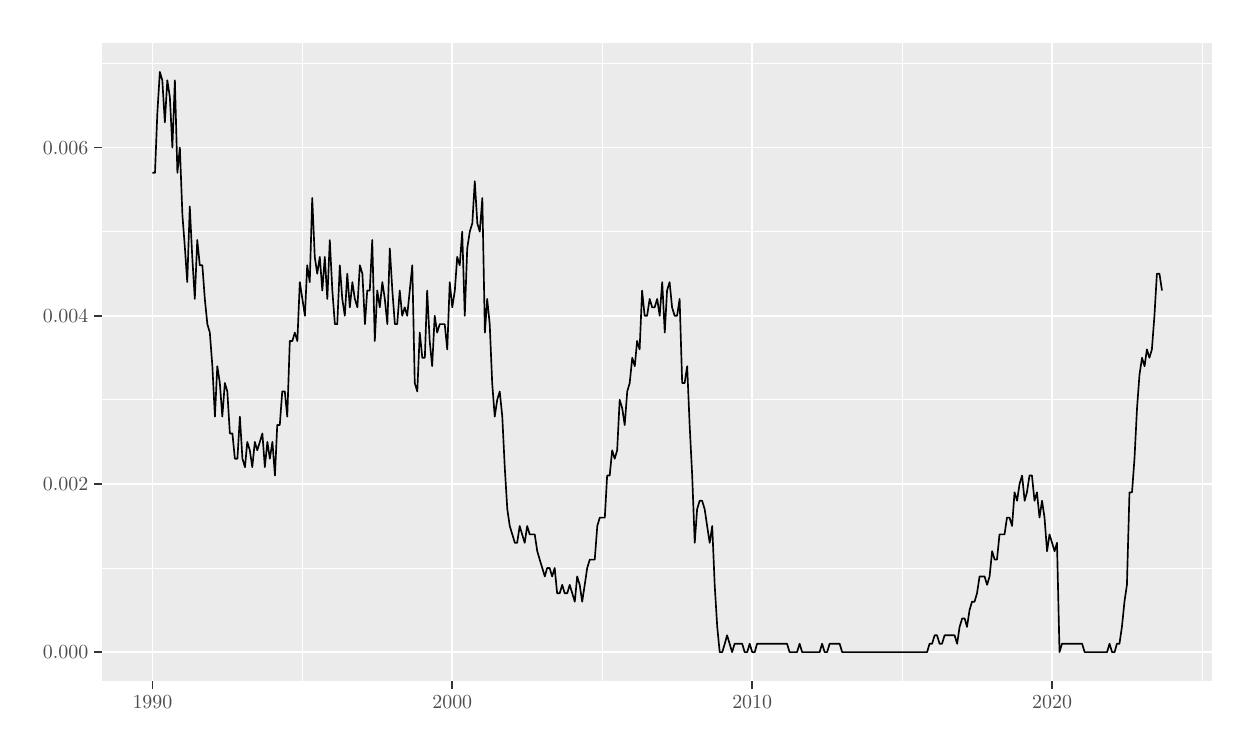
\begin{tikzpicture}[x=1pt,y=1pt]
\definecolor{fillColor}{RGB}{255,255,255}
\path[use as bounding box,fill=fillColor,fill opacity=0.00] (0,0) rectangle (433.62,252.94);
\begin{scope}
\path[clip] (  0.00,  0.00) rectangle (433.62,252.94);
\definecolor{drawColor}{RGB}{255,255,255}
\definecolor{fillColor}{RGB}{255,255,255}

\path[draw=drawColor,line width= 0.6pt,line join=round,line cap=round,fill=fillColor] (  0.00,  0.00) rectangle (433.62,252.94);
\end{scope}
\begin{scope}
\path[clip] ( 26.85, 16.81) rectangle (428.12,247.44);
\definecolor{fillColor}{gray}{0.92}

\path[fill=fillColor] ( 26.85, 16.81) rectangle (428.12,247.44);
\definecolor{drawColor}{RGB}{255,255,255}

\path[draw=drawColor,line width= 0.3pt,line join=round] ( 26.85, 57.68) --
	(428.12, 57.68);

\path[draw=drawColor,line width= 0.3pt,line join=round] ( 26.85,118.45) --
	(428.12,118.45);

\path[draw=drawColor,line width= 0.3pt,line join=round] ( 26.85,179.23) --
	(428.12,179.23);

\path[draw=drawColor,line width= 0.3pt,line join=round] ( 26.85,240.00) --
	(428.12,240.00);

\path[draw=drawColor,line width= 0.3pt,line join=round] ( 99.26, 16.81) --
	( 99.26,247.44);

\path[draw=drawColor,line width= 0.3pt,line join=round] (207.62, 16.81) --
	(207.62,247.44);

\path[draw=drawColor,line width= 0.3pt,line join=round] (315.98, 16.81) --
	(315.98,247.44);

\path[draw=drawColor,line width= 0.3pt,line join=round] (424.33, 16.81) --
	(424.33,247.44);

\path[draw=drawColor,line width= 0.6pt,line join=round] ( 26.85, 27.29) --
	(428.12, 27.29);

\path[draw=drawColor,line width= 0.6pt,line join=round] ( 26.85, 88.07) --
	(428.12, 88.07);

\path[draw=drawColor,line width= 0.6pt,line join=round] ( 26.85,148.84) --
	(428.12,148.84);

\path[draw=drawColor,line width= 0.6pt,line join=round] ( 26.85,209.61) --
	(428.12,209.61);

\path[draw=drawColor,line width= 0.6pt,line join=round] ( 45.09, 16.81) --
	( 45.09,247.44);

\path[draw=drawColor,line width= 0.6pt,line join=round] (153.43, 16.81) --
	(153.43,247.44);

\path[draw=drawColor,line width= 0.6pt,line join=round] (261.81, 16.81) --
	(261.81,247.44);

\path[draw=drawColor,line width= 0.6pt,line join=round] (370.16, 16.81) --
	(370.16,247.44);
\definecolor{drawColor}{RGB}{0,0,0}

\path[draw=drawColor,line width= 0.6pt,line join=round] ( 45.09,200.50) --
	( 46.01,200.50) --
	( 46.84,221.77) --
	( 47.76,236.96) --
	( 48.65,233.92) --
	( 49.57,218.73) --
	( 50.46,233.92) --
	( 51.38,227.85) --
	( 52.29,209.61) --
	( 53.19,233.92) --
	( 54.10,200.50) --
	( 54.99,209.61) --
	( 55.91,185.30) --
	( 56.83,173.15) --
	( 57.66,160.99) --
	( 58.58,188.34) --
	( 59.47,170.11) --
	( 60.39,154.92) --
	( 61.28,176.19) --
	( 62.20,167.07) --
	( 63.12,167.07) --
	( 64.01,154.92) --
	( 64.93,145.80) --
	( 65.82,142.76) --
	( 66.74,130.61) --
	( 67.66,112.38) --
	( 68.52,130.61) --
	( 69.44,124.53) --
	( 70.33,112.38) --
	( 71.25,124.53) --
	( 72.14,121.49) --
	( 73.06,106.30) --
	( 73.98,106.30) --
	( 74.87, 97.18) --
	( 75.79, 97.18) --
	( 76.68,112.38) --
	( 77.60, 97.18) --
	( 78.52, 94.14) --
	( 79.35,103.26) --
	( 80.27,100.22) --
	( 81.16, 94.14) --
	( 82.08,103.26) --
	( 82.97,100.22) --
	( 83.89,103.26) --
	( 84.81,106.30) --
	( 85.70, 94.14) --
	( 86.62,103.26) --
	( 87.51, 97.18) --
	( 88.43,103.26) --
	( 89.35, 91.10) --
	( 90.18,109.34) --
	( 91.10,109.34) --
	( 91.99,121.49) --
	( 92.91,121.49) --
	( 93.80,112.38) --
	( 94.72,139.72) --
	( 95.64,139.72) --
	( 96.53,142.76) --
	( 97.45,139.72) --
	( 98.34,160.99) --
	( 99.26,154.92) --
	(100.18,148.84) --
	(101.01,167.07) --
	(101.93,160.99) --
	(102.82,191.38) --
	(103.74,170.11) --
	(104.63,164.03) --
	(105.55,170.11) --
	(106.47,157.96) --
	(107.36,170.11) --
	(108.28,154.92) --
	(109.17,176.19) --
	(110.09,157.96) --
	(111.01,145.80) --
	(111.87,145.80) --
	(112.79,167.07) --
	(113.68,154.92) --
	(114.60,148.84) --
	(115.49,164.03) --
	(116.41,151.88) --
	(117.33,160.99) --
	(118.22,154.92) --
	(119.14,151.88) --
	(120.03,167.07) --
	(120.95,164.03) --
	(121.87,145.80) --
	(122.70,157.96) --
	(123.62,157.96) --
	(124.51,176.19) --
	(125.43,139.72) --
	(126.32,157.96) --
	(127.24,151.88) --
	(128.16,160.99) --
	(129.05,154.92) --
	(129.97,145.80) --
	(130.86,173.15) --
	(131.77,157.96) --
	(132.69,145.80) --
	(133.53,145.80) --
	(134.44,157.96) --
	(135.34,148.84) --
	(136.25,151.88) --
	(137.14,148.84) --
	(138.06,157.96) --
	(138.98,167.07) --
	(139.87,124.53) --
	(140.79,121.49) --
	(141.68,142.76) --
	(142.60,133.65) --
	(143.52,133.65) --
	(144.35,157.96) --
	(145.27,139.72) --
	(146.16,130.61) --
	(147.08,148.84) --
	(147.97,142.76) --
	(148.89,145.80) --
	(149.81,145.80) --
	(150.70,145.80) --
	(151.62,136.68) --
	(152.51,160.99) --
	(153.43,151.88) --
	(154.35,157.96) --
	(155.21,170.11) --
	(156.13,167.07) --
	(157.02,179.23) --
	(157.94,148.84) --
	(158.83,173.15) --
	(159.75,179.23) --
	(160.67,182.27) --
	(161.56,197.46) --
	(162.48,182.27) --
	(163.37,179.23) --
	(164.29,191.38) --
	(165.21,142.76) --
	(166.04,154.92) --
	(166.96,145.80) --
	(167.85,124.53) --
	(168.77,112.38) --
	(169.66,118.45) --
	(170.58,121.49) --
	(171.50,112.38) --
	(172.39, 94.14) --
	(173.31, 78.95) --
	(174.20, 72.87) --
	(175.12, 69.83) --
	(176.04, 66.79) --
	(176.87, 66.79) --
	(177.79, 72.87) --
	(178.68, 69.83) --
	(179.60, 66.79) --
	(180.49, 72.87) --
	(181.41, 69.83) --
	(182.33, 69.83) --
	(183.22, 69.83) --
	(184.14, 63.76) --
	(185.03, 60.72) --
	(185.95, 57.68) --
	(186.87, 54.64) --
	(187.70, 57.68) --
	(188.62, 57.68) --
	(189.51, 54.64) --
	(190.43, 57.68) --
	(191.32, 48.56) --
	(192.24, 48.56) --
	(193.16, 51.60) --
	(194.05, 48.56) --
	(194.97, 48.56) --
	(195.86, 51.60) --
	(196.78, 48.56) --
	(197.70, 45.52) --
	(198.56, 54.64) --
	(199.48, 51.60) --
	(200.37, 45.52) --
	(201.29, 51.60) --
	(202.18, 57.68) --
	(203.10, 60.72) --
	(204.02, 60.72) --
	(204.91, 60.72) --
	(205.83, 72.87) --
	(206.72, 75.91) --
	(207.64, 75.91) --
	(208.55, 75.91) --
	(209.39, 91.10) --
	(210.31, 91.10) --
	(211.20,100.22) --
	(212.12, 97.18) --
	(213.01,100.22) --
	(213.92,118.45) --
	(214.84,115.41) --
	(215.73,109.34) --
	(216.65,121.49) --
	(217.54,124.53) --
	(218.46,133.65) --
	(219.38,130.61) --
	(220.21,139.72) --
	(221.13,136.68) --
	(222.02,157.96) --
	(222.94,148.84) --
	(223.83,148.84) --
	(224.75,154.92) --
	(225.67,151.88) --
	(226.56,151.88) --
	(227.48,154.92) --
	(228.37,148.84) --
	(229.29,160.99) --
	(230.21,142.76) --
	(231.04,157.96) --
	(231.96,160.99) --
	(232.85,151.88) --
	(233.77,148.84) --
	(234.66,148.84) --
	(235.58,154.92) --
	(236.50,124.53) --
	(237.39,124.53) --
	(238.31,130.61) --
	(239.20,109.34) --
	(240.12, 91.10) --
	(241.04, 66.79) --
	(241.90, 78.95) --
	(242.82, 81.99) --
	(243.71, 81.99) --
	(244.63, 78.95) --
	(245.52, 72.87) --
	(246.44, 66.79) --
	(247.36, 72.87) --
	(248.25, 51.60) --
	(249.17, 36.41) --
	(250.06, 27.29) --
	(250.98, 27.29) --
	(251.90, 30.33) --
	(252.73, 33.37) --
	(253.65, 30.33) --
	(254.54, 27.29) --
	(255.46, 30.33) --
	(256.35, 30.33) --
	(257.27, 30.33) --
	(258.19, 30.33) --
	(259.08, 27.29) --
	(260.00, 27.29) --
	(260.89, 30.33) --
	(261.81, 27.29) --
	(262.73, 27.29) --
	(263.56, 30.33) --
	(264.48, 30.33) --
	(265.37, 30.33) --
	(266.29, 30.33) --
	(267.18, 30.33) --
	(268.10, 30.33) --
	(269.02, 30.33) --
	(269.91, 30.33) --
	(270.83, 30.33) --
	(271.72, 30.33) --
	(272.64, 30.33) --
	(273.56, 30.33) --
	(274.39, 30.33) --
	(275.31, 27.29) --
	(276.20, 27.29) --
	(277.12, 27.29) --
	(278.01, 27.29) --
	(278.93, 30.33) --
	(279.85, 27.29) --
	(280.74, 27.29) --
	(281.66, 27.29) --
	(282.55, 27.29) --
	(283.47, 27.29) --
	(284.39, 27.29) --
	(285.25, 27.29) --
	(286.17, 27.29) --
	(287.06, 30.33) --
	(287.98, 27.29) --
	(288.87, 27.29) --
	(289.79, 30.33) --
	(290.70, 30.33) --
	(291.59, 30.33) --
	(292.51, 30.33) --
	(293.40, 30.33) --
	(294.32, 27.29) --
	(295.24, 27.29) --
	(296.07, 27.29) --
	(296.99, 27.29) --
	(297.88, 27.29) --
	(298.80, 27.29) --
	(299.69, 27.29) --
	(300.61, 27.29) --
	(301.53, 27.29) --
	(302.42, 27.29) --
	(303.34, 27.29) --
	(304.23, 27.29) --
	(305.15, 27.29) --
	(306.07, 27.29) --
	(306.90, 27.29) --
	(307.82, 27.29) --
	(308.71, 27.29) --
	(309.63, 27.29) --
	(310.52, 27.29) --
	(311.44, 27.29) --
	(312.36, 27.29) --
	(313.25, 27.29) --
	(314.17, 27.29) --
	(315.06, 27.29) --
	(315.98, 27.29) --
	(316.90, 27.29) --
	(317.73, 27.29) --
	(318.65, 27.29) --
	(319.54, 27.29) --
	(320.46, 27.29) --
	(321.35, 27.29) --
	(322.27, 27.29) --
	(323.19, 27.29) --
	(324.08, 27.29) --
	(325.00, 27.29) --
	(325.89, 30.33) --
	(326.81, 30.33) --
	(327.73, 33.37) --
	(328.59, 33.37) --
	(329.51, 30.33) --
	(330.40, 30.33) --
	(331.32, 33.37) --
	(332.21, 33.37) --
	(333.13, 33.37) --
	(334.05, 33.37) --
	(334.94, 33.37) --
	(335.86, 30.33) --
	(336.75, 36.41) --
	(337.67, 39.45) --
	(338.59, 39.45) --
	(339.42, 36.41) --
	(340.34, 42.49) --
	(341.23, 45.52) --
	(342.15, 45.52) --
	(343.04, 48.56) --
	(343.96, 54.64) --
	(344.88, 54.64) --
	(345.77, 54.64) --
	(346.69, 51.60) --
	(347.58, 54.64) --
	(348.50, 63.76) --
	(349.42, 60.72) --
	(350.25, 60.72) --
	(351.17, 69.83) --
	(352.06, 69.83) --
	(352.98, 69.83) --
	(353.87, 75.91) --
	(354.79, 75.91) --
	(355.71, 72.87) --
	(356.60, 85.03) --
	(357.52, 81.99) --
	(358.41, 88.07) --
	(359.33, 91.10) --
	(360.25, 81.99) --
	(361.08, 85.03) --
	(362.00, 91.10) --
	(362.89, 91.10) --
	(363.81, 81.99) --
	(364.70, 85.03) --
	(365.62, 75.91) --
	(366.54, 81.99) --
	(367.43, 75.91) --
	(368.35, 63.76) --
	(369.24, 69.83) --
	(370.16, 66.79) --
	(371.07, 63.76) --
	(371.94, 66.79) --
	(372.85, 27.29) --
	(373.74, 30.33) --
	(374.66, 30.33) --
	(375.55, 30.33) --
	(376.47, 30.33) --
	(377.39, 30.33) --
	(378.28, 30.33) --
	(379.20, 30.33) --
	(380.09, 30.33) --
	(381.01, 30.33) --
	(381.93, 27.29) --
	(382.76, 27.29) --
	(383.68, 27.29) --
	(384.57, 27.29) --
	(385.49, 27.29) --
	(386.38, 27.29) --
	(387.30, 27.29) --
	(388.22, 27.29) --
	(389.11, 27.29) --
	(390.03, 27.29) --
	(390.92, 30.33) --
	(391.84, 27.29) --
	(392.76, 27.29) --
	(393.59, 30.33) --
	(394.51, 30.33) --
	(395.40, 36.41) --
	(396.32, 45.52) --
	(397.21, 51.60) --
	(398.13, 85.03) --
	(399.05, 85.03) --
	(399.94, 97.18) --
	(400.86,115.41) --
	(401.75,127.57) --
	(402.67,133.65) --
	(403.59,130.61) --
	(404.42,136.68) --
	(405.34,133.65) --
	(406.23,136.68) --
	(407.15,148.84) --
	(408.04,164.03) --
	(408.96,164.03) --
	(409.88,157.96);
\end{scope}
\begin{scope}
\path[clip] (  0.00,  0.00) rectangle (433.62,252.94);
\definecolor{drawColor}{gray}{0.30}

\node[text=drawColor,anchor=base east,inner sep=0pt, outer sep=0pt, scale=  0.72] at ( 21.90, 24.81) {0.000};

\node[text=drawColor,anchor=base east,inner sep=0pt, outer sep=0pt, scale=  0.72] at ( 21.90, 85.59) {0.002};

\node[text=drawColor,anchor=base east,inner sep=0pt, outer sep=0pt, scale=  0.72] at ( 21.90,146.36) {0.004};

\node[text=drawColor,anchor=base east,inner sep=0pt, outer sep=0pt, scale=  0.72] at ( 21.90,207.13) {0.006};
\end{scope}
\begin{scope}
\path[clip] (  0.00,  0.00) rectangle (433.62,252.94);
\definecolor{drawColor}{gray}{0.20}

\path[draw=drawColor,line width= 0.6pt,line join=round] ( 24.10, 27.29) --
	( 26.85, 27.29);

\path[draw=drawColor,line width= 0.6pt,line join=round] ( 24.10, 88.07) --
	( 26.85, 88.07);

\path[draw=drawColor,line width= 0.6pt,line join=round] ( 24.10,148.84) --
	( 26.85,148.84);

\path[draw=drawColor,line width= 0.6pt,line join=round] ( 24.10,209.61) --
	( 26.85,209.61);
\end{scope}
\begin{scope}
\path[clip] (  0.00,  0.00) rectangle (433.62,252.94);
\definecolor{drawColor}{gray}{0.20}

\path[draw=drawColor,line width= 0.6pt,line join=round] ( 45.09, 14.06) --
	( 45.09, 16.81);

\path[draw=drawColor,line width= 0.6pt,line join=round] (153.43, 14.06) --
	(153.43, 16.81);

\path[draw=drawColor,line width= 0.6pt,line join=round] (261.81, 14.06) --
	(261.81, 16.81);

\path[draw=drawColor,line width= 0.6pt,line join=round] (370.16, 14.06) --
	(370.16, 16.81);
\end{scope}
\begin{scope}
\path[clip] (  0.00,  0.00) rectangle (433.62,252.94);
\definecolor{drawColor}{gray}{0.30}

\node[text=drawColor,anchor=base,inner sep=0pt, outer sep=0pt, scale=  0.72] at ( 45.09,  6.90) {1990};

\node[text=drawColor,anchor=base,inner sep=0pt, outer sep=0pt, scale=  0.72] at (153.43,  6.90) {2000};

\node[text=drawColor,anchor=base,inner sep=0pt, outer sep=0pt, scale=  0.72] at (261.81,  6.90) {2010};

\node[text=drawColor,anchor=base,inner sep=0pt, outer sep=0pt, scale=  0.72] at (370.16,  6.90) {2020};
\end{scope}
\end{tikzpicture}

\label{plot:rf_ts}
\end{figure}

\begin{figure}[H]
\centering
\caption[Time series of the mean cross-sectional properties]{\textbf{Time series of the mean cross-sectional properties \textnormal{- Own source}}\\ Figure plots development of the firm characteristics across time. The values shown are the monthly cross-sectional averages. The construction of each variable is explained in detail in Section \ref{Data}.}
% Created by tikzDevice version 0.12.6 on 2024-03-27 12:49:17
% !TEX encoding = UTF-8 Unicode
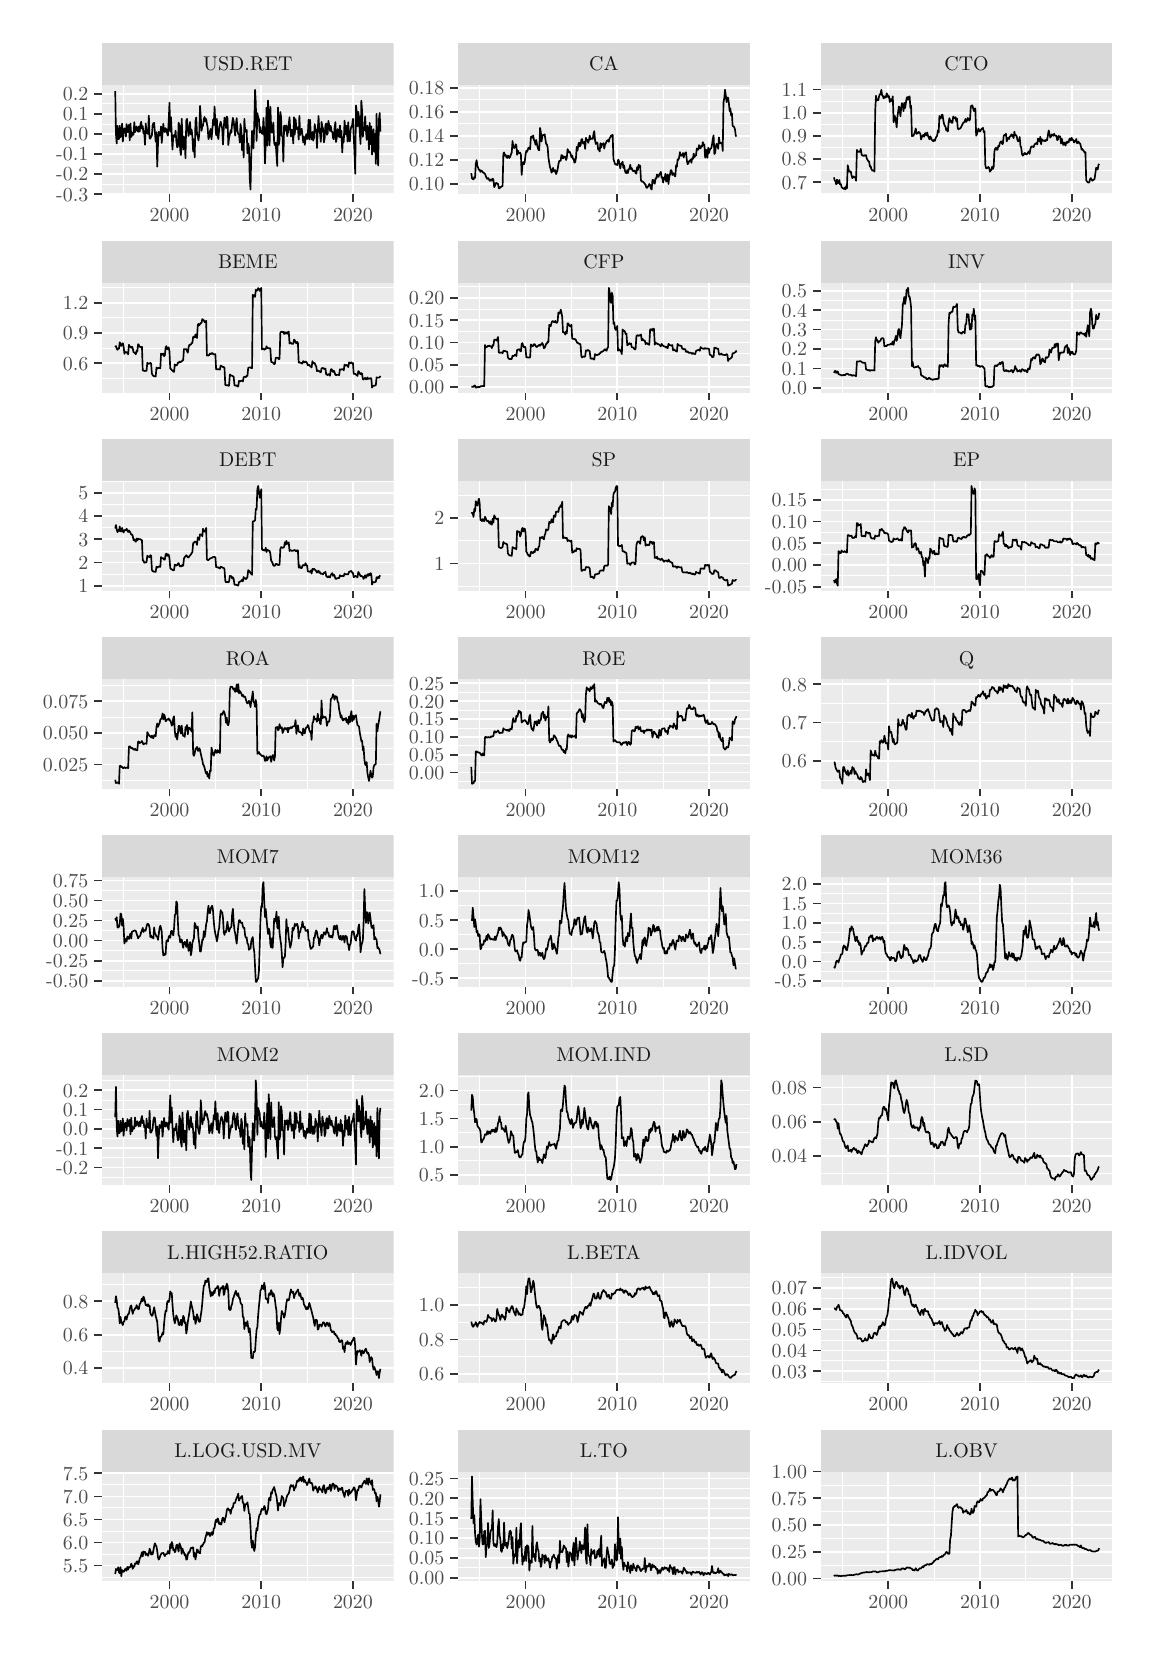
\begin{tikzpicture}[x=1pt,y=1pt]
\definecolor{fillColor}{RGB}{255,255,255}
\path[use as bounding box,fill=fillColor,fill opacity=0.00] (0,0) rectangle (397.48,578.16);
\begin{scope}
\path[clip] (  0.00,  0.00) rectangle (397.48,578.16);
\definecolor{drawColor}{RGB}{255,255,255}
\definecolor{fillColor}{RGB}{255,255,255}

\path[draw=drawColor,line width= 0.6pt,line join=round,line cap=round,fill=fillColor] (  0.00, -0.00) rectangle (397.48,578.16);
\end{scope}
\begin{scope}
\path[clip] ( 26.85,517.89) rectangle (132.26,557.50);
\definecolor{fillColor}{gray}{0.92}

\path[fill=fillColor] ( 26.85,517.89) rectangle (132.26,557.50);
\definecolor{drawColor}{RGB}{255,255,255}

\path[draw=drawColor,line width= 0.3pt,line join=round] ( 26.85,521.62) --
	(132.26,521.62);

\path[draw=drawColor,line width= 0.3pt,line join=round] ( 26.85,528.87) --
	(132.26,528.87);

\path[draw=drawColor,line width= 0.3pt,line join=round] ( 26.85,536.12) --
	(132.26,536.12);

\path[draw=drawColor,line width= 0.3pt,line join=round] ( 26.85,543.36) --
	(132.26,543.36);

\path[draw=drawColor,line width= 0.3pt,line join=round] ( 26.85,550.61) --
	(132.26,550.61);

\path[draw=drawColor,line width= 0.3pt,line join=round] ( 34.67,517.89) --
	( 34.67,557.50);

\path[draw=drawColor,line width= 0.3pt,line join=round] ( 67.82,517.89) --
	( 67.82,557.50);

\path[draw=drawColor,line width= 0.3pt,line join=round] (100.97,517.89) --
	(100.97,557.50);

\path[draw=drawColor,line width= 0.6pt,line join=round] ( 26.85,517.99) --
	(132.26,517.99);

\path[draw=drawColor,line width= 0.6pt,line join=round] ( 26.85,525.24) --
	(132.26,525.24);

\path[draw=drawColor,line width= 0.6pt,line join=round] ( 26.85,532.49) --
	(132.26,532.49);

\path[draw=drawColor,line width= 0.6pt,line join=round] ( 26.85,539.74) --
	(132.26,539.74);

\path[draw=drawColor,line width= 0.6pt,line join=round] ( 26.85,546.99) --
	(132.26,546.99);

\path[draw=drawColor,line width= 0.6pt,line join=round] ( 26.85,554.24) --
	(132.26,554.24);

\path[draw=drawColor,line width= 0.6pt,line join=round] ( 51.25,517.89) --
	( 51.25,557.50);

\path[draw=drawColor,line width= 0.6pt,line join=round] ( 84.40,517.89) --
	( 84.40,557.50);

\path[draw=drawColor,line width= 0.6pt,line join=round] (117.54,517.89) --
	(117.54,557.50);
\definecolor{drawColor}{RGB}{0,0,0}

\path[draw=drawColor,line width= 0.6pt,line join=round] ( 31.64,555.24) --
	( 31.89,539.94) --
	( 32.17,536.29) --
	( 32.44,542.69) --
	( 32.73,537.85) --
	( 33.00,537.97) --
	( 33.26,542.74) --
	( 33.56,538.58) --
	( 33.83,539.55) --
	( 34.12,543.49) --
	( 34.39,536.99) --
	( 34.66,540.93) --
	( 34.95,541.79) --
	( 35.20,541.64) --
	( 35.49,538.82) --
	( 35.74,543.30) --
	( 36.04,540.40) --
	( 36.31,541.42) --
	( 36.59,543.04) --
	( 36.87,537.42) --
	( 37.14,543.53) --
	( 37.43,538.67) --
	( 37.70,539.28) --
	( 37.96,540.23) --
	( 38.26,539.46) --
	( 38.53,544.03) --
	( 38.79,540.39) --
	( 39.08,541.44) --
	( 39.36,542.45) --
	( 39.61,541.06) --
	( 39.91,540.53) --
	( 40.19,542.45) --
	( 40.47,540.64) --
	( 40.75,543.10) --
	( 41.01,544.14) --
	( 41.30,541.67) --
	( 41.58,542.57) --
	( 41.84,539.92) --
	( 42.12,540.71) --
	( 42.39,535.85) --
	( 42.66,543.57) --
	( 42.95,539.97) --
	( 43.23,541.18) --
	( 43.49,539.73) --
	( 43.78,546.37) --
	( 44.06,538.18) --
	( 44.32,538.06) --
	( 44.61,538.79) --
	( 44.89,539.27) --
	( 45.14,542.90) --
	( 45.43,543.65) --
	( 45.70,543.73) --
	( 45.97,540.36) --
	( 46.26,536.97) --
	( 46.54,540.37) --
	( 46.82,527.93) --
	( 47.09,536.03) --
	( 47.36,540.55) --
	( 47.65,539.33) --
	( 47.93,539.26) --
	( 48.19,542.45) --
	( 48.44,536.51) --
	( 48.74,540.35) --
	( 49.02,543.42) --
	( 49.30,540.67) --
	( 49.57,540.44) --
	( 49.84,541.84) --
	( 50.13,541.21) --
	( 50.40,539.93) --
	( 50.67,539.14) --
	( 50.96,544.46) --
	( 51.24,551.06) --
	( 51.52,540.64) --
	( 51.78,545.79) --
	( 52.07,539.43) --
	( 52.32,534.12) --
	( 52.62,539.13) --
	( 52.89,539.36) --
	( 53.17,538.69) --
	( 53.45,540.95) --
	( 53.72,537.07) --
	( 54.01,534.90) --
	( 54.28,535.23) --
	( 54.54,543.83) --
	( 54.84,542.77) --
	( 55.10,534.04) --
	( 55.37,532.14) --
	( 55.65,545.23) --
	( 55.93,538.84) --
	( 56.19,534.08) --
	( 56.48,538.72) --
	( 56.77,536.59) --
	( 57.02,530.93) --
	( 57.32,544.60) --
	( 57.59,545.21) --
	( 57.87,541.35) --
	( 58.15,539.03) --
	( 58.41,541.72) --
	( 58.67,544.04) --
	( 58.96,539.65) --
	( 59.24,541.30) --
	( 59.50,538.96) --
	( 59.80,533.43) --
	( 60.07,537.83) --
	( 60.35,531.27) --
	( 60.63,544.27) --
	( 60.90,545.73) --
	( 61.19,539.81) --
	( 61.47,538.81) --
	( 61.72,537.37) --
	( 62.00,539.65) --
	( 62.27,549.90) --
	( 62.55,545.97) --
	( 62.83,540.90) --
	( 63.11,542.64) --
	( 63.37,542.67) --
	( 63.66,545.22) --
	( 63.94,545.93) --
	( 64.20,544.28) --
	( 64.50,545.16) --
	( 64.77,543.45) --
	( 65.02,542.25) --
	( 65.32,537.89) --
	( 65.60,538.64) --
	( 65.88,540.67) --
	( 66.15,541.56) --
	( 66.42,537.82) --
	( 66.71,541.01) --
	( 66.98,544.88) --
	( 67.25,542.96) --
	( 67.54,549.67) --
	( 67.82,543.18) --
	( 68.10,539.34) --
	( 68.36,545.20) --
	( 68.64,539.04) --
	( 68.90,537.92) --
	( 69.19,541.29) --
	( 69.46,543.13) --
	( 69.73,544.20) --
	( 70.02,543.08) --
	( 70.30,541.60) --
	( 70.58,535.95) --
	( 70.85,541.74) --
	( 71.12,545.64) --
	( 71.41,544.83) --
	( 71.67,541.86) --
	( 71.95,546.03) --
	( 72.20,545.41) --
	( 72.50,535.75) --
	( 72.77,538.34) --
	( 73.06,539.46) --
	( 73.34,541.09) --
	( 73.60,540.18) --
	( 73.89,543.61) --
	( 74.16,545.55) --
	( 74.43,544.43) --
	( 74.73,541.33) --
	( 74.98,539.12) --
	( 75.25,543.32) --
	( 75.53,545.45) --
	( 75.81,540.88) --
	( 76.08,539.74) --
	( 76.37,539.65) --
	( 76.65,536.63) --
	( 76.90,543.32) --
	( 77.20,541.25) --
	( 77.48,533.85) --
	( 77.76,539.11) --
	( 78.04,531.23) --
	( 78.30,545.18) --
	( 78.58,541.02) --
	( 78.85,540.46) --
	( 79.13,541.25) --
	( 79.41,532.72) --
	( 79.69,536.34) --
	( 79.95,535.07) --
	( 80.24,523.65) --
	( 80.52,519.69) --
	( 80.78,531.70) --
	( 81.08,540.88) --
	( 81.35,537.38) --
	( 81.60,534.60) --
	( 81.89,543.95) --
	( 82.17,555.70) --
	( 82.43,551.11) --
	( 82.72,537.22) --
	( 83.00,547.24) --
	( 83.28,545.78) --
	( 83.56,545.09) --
	( 83.83,540.18) --
	( 84.11,542.18) --
	( 84.39,540.43) --
	( 84.65,539.96) --
	( 84.91,539.74) --
	( 85.21,545.56) --
	( 85.48,540.39) --
	( 85.76,529.09) --
	( 86.03,537.22) --
	( 86.31,549.24) --
	( 86.60,535.48) --
	( 86.87,551.86) --
	( 87.13,542.66) --
	( 87.42,535.58) --
	( 87.70,549.58) --
	( 87.98,541.84) --
	( 88.24,540.19) --
	( 88.52,541.86) --
	( 88.78,543.86) --
	( 89.07,536.44) --
	( 89.35,535.64) --
	( 89.61,536.59) --
	( 89.91,532.07) --
	( 90.18,528.15) --
	( 90.46,549.35) --
	( 90.73,535.79) --
	( 91.01,537.61) --
	( 91.30,547.68) --
	( 91.56,545.95) --
	( 91.83,539.03) --
	( 92.11,538.83) --
	( 92.39,529.74) --
	( 92.66,542.87) --
	( 92.95,540.86) --
	( 93.23,542.55) --
	( 93.48,542.87) --
	( 93.78,538.95) --
	( 94.06,540.34) --
	( 94.34,543.36) --
	( 94.62,545.82) --
	( 94.87,541.35) --
	( 95.14,538.82) --
	( 95.43,541.27) --
	( 95.71,540.93) --
	( 95.96,536.26) --
	( 96.26,545.78) --
	( 96.53,539.54) --
	( 96.81,545.11) --
	( 97.10,541.73) --
	( 97.36,541.43) --
	( 97.65,542.10) --
	( 97.93,537.71) --
	( 98.18,546.29) --
	( 98.47,539.37) --
	( 98.74,541.37) --
	( 99.01,541.60) --
	( 99.29,539.46) --
	( 99.57,536.70) --
	( 99.84,538.77) --
	(100.13,535.81) --
	(100.41,538.10) --
	(100.66,539.75) --
	(100.96,537.88) --
	(101.23,539.25) --
	(101.49,544.94) --
	(101.78,537.72) --
	(102.05,544.87) --
	(102.31,539.42) --
	(102.60,537.76) --
	(102.89,540.47) --
	(103.17,537.34) --
	(103.44,538.22) --
	(103.71,543.28) --
	(103.99,541.62) --
	(104.27,541.27) --
	(104.54,534.67) --
	(104.82,540.99) --
	(105.10,546.23) --
	(105.36,541.47) --
	(105.65,539.87) --
	(105.93,536.88) --
	(106.19,544.08) --
	(106.49,542.25) --
	(106.76,541.68) --
	(107.04,536.70) --
	(107.31,538.11) --
	(107.59,542.97) --
	(107.88,543.52) --
	(108.13,539.45) --
	(108.41,539.89) --
	(108.67,544.46) --
	(108.97,542.76) --
	(109.24,540.86) --
	(109.52,542.63) --
	(109.80,540.58) --
	(110.06,540.55) --
	(110.35,538.33) --
	(110.63,537.77) --
	(110.89,541.75) --
	(111.19,544.06) --
	(111.44,536.85) --
	(111.72,538.54) --
	(112.00,541.51) --
	(112.28,540.02) --
	(112.54,538.60) --
	(112.83,542.83) --
	(113.11,538.47) --
	(113.37,540.85) --
	(113.67,533.08) --
	(113.94,538.58) --
	(114.22,536.82) --
	(114.50,544.54) --
	(114.76,541.56) --
	(115.02,539.52) --
	(115.31,542.76) --
	(115.59,536.99) --
	(115.84,544.02) --
	(116.14,537.37) --
	(116.42,537.09) --
	(116.70,541.34) --
	(116.98,542.49) --
	(117.24,542.84) --
	(117.53,545.23) --
	(117.81,538.74) --
	(118.07,533.74) --
	(118.36,525.37) --
	(118.63,550.03) --
	(118.89,548.03) --
	(119.18,542.48) --
	(119.47,547.71) --
	(119.75,545.62) --
	(120.02,539.88) --
	(120.29,536.12) --
	(120.57,551.78) --
	(120.85,547.90) --
	(121.12,538.73) --
	(121.37,541.38) --
	(121.67,541.15) --
	(121.94,546.08) --
	(122.22,541.38) --
	(122.50,537.61) --
	(122.77,542.73) --
	(123.06,541.27) --
	(123.33,534.09) --
	(123.59,543.75) --
	(123.89,536.13) --
	(124.17,542.48) --
	(124.45,532.30) --
	(124.70,535.12) --
	(124.98,541.45) --
	(125.25,533.38) --
	(125.54,539.71) --
	(125.81,528.93) --
	(126.07,547.01) --
	(126.37,533.67) --
	(126.64,528.34) --
	(126.93,544.89) --
	(127.20,547.32) --
	(127.47,540.63);
\end{scope}
\begin{scope}
\path[clip] ( 26.85,446.30) rectangle (132.26,485.92);
\definecolor{fillColor}{gray}{0.92}

\path[fill=fillColor] ( 26.85,446.30) rectangle (132.26,485.92);
\definecolor{drawColor}{RGB}{255,255,255}

\path[draw=drawColor,line width= 0.3pt,line join=round] ( 26.85,451.47) --
	(132.26,451.47);

\path[draw=drawColor,line width= 0.3pt,line join=round] ( 26.85,462.38) --
	(132.26,462.38);

\path[draw=drawColor,line width= 0.3pt,line join=round] ( 26.85,473.29) --
	(132.26,473.29);

\path[draw=drawColor,line width= 0.3pt,line join=round] ( 26.85,484.20) --
	(132.26,484.20);

\path[draw=drawColor,line width= 0.3pt,line join=round] ( 34.67,446.30) --
	( 34.67,485.92);

\path[draw=drawColor,line width= 0.3pt,line join=round] ( 67.82,446.30) --
	( 67.82,485.92);

\path[draw=drawColor,line width= 0.3pt,line join=round] (100.97,446.30) --
	(100.97,485.92);

\path[draw=drawColor,line width= 0.6pt,line join=round] ( 26.85,456.93) --
	(132.26,456.93);

\path[draw=drawColor,line width= 0.6pt,line join=round] ( 26.85,467.83) --
	(132.26,467.83);

\path[draw=drawColor,line width= 0.6pt,line join=round] ( 26.85,478.74) --
	(132.26,478.74);

\path[draw=drawColor,line width= 0.6pt,line join=round] ( 51.25,446.30) --
	( 51.25,485.92);

\path[draw=drawColor,line width= 0.6pt,line join=round] ( 84.40,446.30) --
	( 84.40,485.92);

\path[draw=drawColor,line width= 0.6pt,line join=round] (117.54,446.30) --
	(117.54,485.92);
\definecolor{drawColor}{RGB}{0,0,0}

\path[draw=drawColor,line width= 0.6pt,line join=round] ( 31.64,462.71) --
	( 31.89,463.10) --
	( 32.17,462.29) --
	( 32.44,461.75) --
	( 32.73,462.25) --
	( 33.00,462.21) --
	( 33.26,464.46) --
	( 33.56,463.98) --
	( 33.83,463.15) --
	( 34.12,463.55) --
	( 34.39,464.13) --
	( 34.66,462.99) --
	( 34.95,460.30) --
	( 35.20,460.98) --
	( 35.49,460.82) --
	( 35.74,460.97) --
	( 36.04,460.51) --
	( 36.31,460.14) --
	( 36.59,463.58) --
	( 36.87,463.03) --
	( 37.14,462.81) --
	( 37.43,462.51) --
	( 37.70,462.87) --
	( 37.96,462.29) --
	( 38.26,460.84) --
	( 38.53,460.82) --
	( 38.79,460.56) --
	( 39.08,460.13) --
	( 39.36,461.39) --
	( 39.61,461.10) --
	( 39.91,463.79) --
	( 40.19,463.46) --
	( 40.47,462.83) --
	( 40.75,462.79) --
	( 41.01,462.58) --
	( 41.30,462.82) --
	( 41.58,454.32) --
	( 41.84,454.21) --
	( 42.12,454.13) --
	( 42.39,454.10) --
	( 42.66,454.26) --
	( 42.95,454.10) --
	( 43.23,457.06) --
	( 43.49,456.62) --
	( 43.78,456.88) --
	( 44.06,456.76) --
	( 44.32,457.04) --
	( 44.61,456.73) --
	( 44.89,453.13) --
	( 45.14,452.67) --
	( 45.43,452.30) --
	( 45.70,452.14) --
	( 45.97,452.21) --
	( 46.26,452.10) --
	( 46.54,455.34) --
	( 46.82,454.93) --
	( 47.09,455.19) --
	( 47.36,455.12) --
	( 47.65,455.35) --
	( 47.93,455.06) --
	( 48.19,460.39) --
	( 48.44,459.84) --
	( 48.74,460.32) --
	( 49.02,460.38) --
	( 49.30,459.43) --
	( 49.57,459.78) --
	( 49.84,462.56) --
	( 50.13,463.10) --
	( 50.40,461.89) --
	( 50.67,462.45) --
	( 50.96,462.59) --
	( 51.24,461.10) --
	( 51.52,454.95) --
	( 51.78,454.79) --
	( 52.07,454.38) --
	( 52.32,454.30) --
	( 52.62,453.89) --
	( 52.89,453.76) --
	( 53.17,456.50) --
	( 53.45,456.10) --
	( 53.72,456.12) --
	( 54.01,456.32) --
	( 54.28,457.11) --
	( 54.54,457.02) --
	( 54.84,457.50) --
	( 55.10,457.21) --
	( 55.37,457.45) --
	( 55.65,457.51) --
	( 55.93,457.91) --
	( 56.19,457.98) --
	( 56.48,462.00) --
	( 56.77,461.93) --
	( 57.02,461.99) --
	( 57.32,462.00) --
	( 57.59,461.34) --
	( 57.87,460.70) --
	( 58.15,462.65) --
	( 58.41,463.50) --
	( 58.67,463.61) --
	( 58.96,463.59) --
	( 59.24,464.19) --
	( 59.50,464.19) --
	( 59.80,466.44) --
	( 60.07,466.44) --
	( 60.35,466.20) --
	( 60.63,467.31) --
	( 60.90,466.28) --
	( 61.19,466.02) --
	( 61.47,470.68) --
	( 61.72,471.12) --
	( 62.00,470.57) --
	( 62.27,471.10) --
	( 62.55,471.41) --
	( 62.83,471.47) --
	( 63.11,472.86) --
	( 63.37,472.59) --
	( 63.66,472.41) --
	( 63.94,471.76) --
	( 64.20,471.97) --
	( 64.50,472.22) --
	( 64.77,459.67) --
	( 65.02,459.81) --
	( 65.32,459.64) --
	( 65.60,459.92) --
	( 65.88,460.42) --
	( 66.15,460.17) --
	( 66.42,460.44) --
	( 66.71,460.62) --
	( 66.98,460.26) --
	( 67.25,460.06) --
	( 67.54,460.13) --
	( 67.82,460.21) --
	( 68.10,454.66) --
	( 68.36,454.74) --
	( 68.64,454.77) --
	( 68.90,454.71) --
	( 69.19,454.68) --
	( 69.46,454.57) --
	( 69.73,456.06) --
	( 70.02,455.84) --
	( 70.30,455.73) --
	( 70.58,455.51) --
	( 70.85,455.53) --
	( 71.12,455.20) --
	( 71.41,449.03) --
	( 71.67,448.96) --
	( 71.95,448.91) --
	( 72.20,449.02) --
	( 72.50,448.73) --
	( 72.77,448.78) --
	( 73.06,452.86) --
	( 73.34,452.47) --
	( 73.60,452.49) --
	( 73.89,452.32) --
	( 74.16,452.22) --
	( 74.43,452.02) --
	( 74.73,448.92) --
	( 74.98,448.85) --
	( 75.25,448.89) --
	( 75.53,448.83) --
	( 75.81,448.50) --
	( 76.08,448.53) --
	( 76.37,450.53) --
	( 76.65,450.42) --
	( 76.90,450.39) --
	( 77.20,450.60) --
	( 77.48,450.55) --
	( 77.76,450.32) --
	( 78.04,451.82) --
	( 78.30,452.00) --
	( 78.58,451.99) --
	( 78.85,451.85) --
	( 79.13,452.39) --
	( 79.41,452.30) --
	( 79.69,455.24) --
	( 79.95,455.33) --
	( 80.24,455.42) --
	( 80.52,455.35) --
	( 80.78,455.18) --
	( 81.08,455.14) --
	( 81.35,481.63) --
	( 81.60,480.83) --
	( 81.89,481.53) --
	( 82.17,480.87) --
	( 82.43,483.47) --
	( 82.72,483.03) --
	( 83.00,483.29) --
	( 83.28,484.03) --
	( 83.56,483.84) --
	( 83.83,483.08) --
	( 84.11,483.53) --
	( 84.39,484.12) --
	( 84.65,461.87) --
	( 84.91,462.14) --
	( 85.21,462.13) --
	( 85.48,461.78) --
	( 85.76,462.06) --
	( 86.03,462.05) --
	( 86.31,463.01) --
	( 86.60,462.34) --
	( 86.87,462.41) --
	( 87.13,462.21) --
	( 87.42,462.43) --
	( 87.70,462.08) --
	( 87.98,457.37) --
	( 88.24,457.34) --
	( 88.52,457.21) --
	( 88.78,456.94) --
	( 89.07,456.55) --
	( 89.35,456.78) --
	( 89.61,458.80) --
	( 89.91,458.88) --
	( 90.18,458.88) --
	( 90.46,458.87) --
	( 90.73,458.36) --
	( 91.01,458.46) --
	( 91.30,467.89) --
	( 91.56,468.26) --
	( 91.83,468.28) --
	( 92.11,468.07) --
	( 92.39,468.25) --
	( 92.66,467.45) --
	( 92.95,468.12) --
	( 93.23,467.62) --
	( 93.48,468.03) --
	( 93.78,467.53) --
	( 94.06,468.21) --
	( 94.34,468.32) --
	( 94.62,463.99) --
	( 94.87,464.45) --
	( 95.14,464.19) --
	( 95.43,463.94) --
	( 95.71,463.87) --
	( 95.96,463.95) --
	( 96.26,465.41) --
	( 96.53,465.20) --
	( 96.81,464.45) --
	( 97.10,464.08) --
	( 97.36,464.61) --
	( 97.65,464.18) --
	( 97.93,457.15) --
	( 98.18,457.32) --
	( 98.47,457.02) --
	( 98.74,457.10) --
	( 99.01,456.79) --
	( 99.29,456.83) --
	( 99.57,457.67) --
	( 99.84,457.38) --
	(100.13,457.21) --
	(100.41,457.52) --
	(100.66,457.35) --
	(100.96,456.94) --
	(101.23,456.14) --
	(101.49,456.35) --
	(101.78,456.28) --
	(102.05,455.82) --
	(102.31,455.72) --
	(102.60,455.35) --
	(102.89,457.64) --
	(103.17,456.99) --
	(103.44,456.91) --
	(103.71,456.98) --
	(103.99,456.19) --
	(104.27,455.73) --
	(104.54,454.03) --
	(104.82,454.16) --
	(105.10,454.21) --
	(105.36,454.03) --
	(105.65,453.75) --
	(105.93,453.61) --
	(106.19,455.04) --
	(106.49,455.15) --
	(106.76,455.17) --
	(107.04,454.91) --
	(107.31,454.76) --
	(107.59,454.99) --
	(107.88,452.81) --
	(108.13,452.95) --
	(108.41,452.62) --
	(108.67,453.00) --
	(108.97,452.88) --
	(109.24,452.37) --
	(109.52,454.58) --
	(109.80,454.77) --
	(110.06,454.25) --
	(110.35,453.75) --
	(110.63,454.18) --
	(110.89,453.63) --
	(111.19,452.72) --
	(111.44,452.58) --
	(111.72,452.72) --
	(112.00,452.75) --
	(112.28,452.71) --
	(112.54,452.55) --
	(112.83,454.72) --
	(113.11,454.55) --
	(113.37,454.68) --
	(113.67,454.81) --
	(113.94,454.63) --
	(114.22,454.35) --
	(114.50,456.40) --
	(114.76,456.21) --
	(115.02,455.98) --
	(115.31,456.27) --
	(115.59,455.91) --
	(115.84,455.50) --
	(116.14,457.19) --
	(116.42,456.99) --
	(116.70,456.97) --
	(116.98,457.23) --
	(117.24,456.81) --
	(117.53,456.97) --
	(117.81,453.08) --
	(118.07,453.13) --
	(118.36,453.10) --
	(118.63,452.74) --
	(118.89,452.71) --
	(119.18,452.30) --
	(119.47,454.06) --
	(119.75,453.75) --
	(120.02,453.20) --
	(120.29,452.96) --
	(120.57,453.35) --
	(120.85,453.02) --
	(121.12,451.11) --
	(121.37,451.00) --
	(121.67,451.36) --
	(121.94,451.61) --
	(122.22,451.13) --
	(122.50,451.08) --
	(122.77,451.75) --
	(123.06,451.24) --
	(123.33,451.31) --
	(123.59,451.33) --
	(123.89,451.57) --
	(124.17,451.39) --
	(124.45,448.10) --
	(124.70,448.70) --
	(124.98,448.74) --
	(125.25,448.79) --
	(125.54,448.85) --
	(125.81,449.01) --
	(126.07,451.78) --
	(126.37,451.73) --
	(126.64,451.69) --
	(126.93,451.69) --
	(127.20,451.86) --
	(127.47,452.29);
\end{scope}
\begin{scope}
\path[clip] ( 26.85,374.72) rectangle (132.26,414.34);
\definecolor{fillColor}{gray}{0.92}

\path[fill=fillColor] ( 26.85,374.72) rectangle (132.26,414.34);
\definecolor{drawColor}{RGB}{255,255,255}

\path[draw=drawColor,line width= 0.3pt,line join=round] ( 26.85,380.69) --
	(132.26,380.69);

\path[draw=drawColor,line width= 0.3pt,line join=round] ( 26.85,389.08) --
	(132.26,389.08);

\path[draw=drawColor,line width= 0.3pt,line join=round] ( 26.85,397.48) --
	(132.26,397.48);

\path[draw=drawColor,line width= 0.3pt,line join=round] ( 26.85,405.88) --
	(132.26,405.88);

\path[draw=drawColor,line width= 0.3pt,line join=round] ( 26.85,414.27) --
	(132.26,414.27);

\path[draw=drawColor,line width= 0.3pt,line join=round] ( 34.67,374.72) --
	( 34.67,414.34);

\path[draw=drawColor,line width= 0.3pt,line join=round] ( 67.82,374.72) --
	( 67.82,414.34);

\path[draw=drawColor,line width= 0.3pt,line join=round] (100.97,374.72) --
	(100.97,414.34);

\path[draw=drawColor,line width= 0.6pt,line join=round] ( 26.85,376.49) --
	(132.26,376.49);

\path[draw=drawColor,line width= 0.6pt,line join=round] ( 26.85,384.89) --
	(132.26,384.89);

\path[draw=drawColor,line width= 0.6pt,line join=round] ( 26.85,393.28) --
	(132.26,393.28);

\path[draw=drawColor,line width= 0.6pt,line join=round] ( 26.85,401.68) --
	(132.26,401.68);

\path[draw=drawColor,line width= 0.6pt,line join=round] ( 26.85,410.07) --
	(132.26,410.07);

\path[draw=drawColor,line width= 0.6pt,line join=round] ( 51.25,374.72) --
	( 51.25,414.34);

\path[draw=drawColor,line width= 0.6pt,line join=round] ( 84.40,374.72) --
	( 84.40,414.34);

\path[draw=drawColor,line width= 0.6pt,line join=round] (117.54,374.72) --
	(117.54,414.34);
\definecolor{drawColor}{RGB}{0,0,0}

\path[draw=drawColor,line width= 0.6pt,line join=round] ( 31.64,397.19) --
	( 31.89,398.43) --
	( 32.17,396.86) --
	( 32.44,395.86) --
	( 32.73,396.63) --
	( 33.00,396.24) --
	( 33.26,397.89) --
	( 33.56,396.17) --
	( 33.83,396.11) --
	( 34.12,397.40) --
	( 34.39,396.23) --
	( 34.66,395.73) --
	( 34.95,396.63) --
	( 35.20,396.57) --
	( 35.49,396.48) --
	( 35.74,397.11) --
	( 36.04,396.44) --
	( 36.31,395.91) --
	( 36.59,396.46) --
	( 36.87,396.09) --
	( 37.14,395.56) --
	( 37.43,394.99) --
	( 37.70,395.05) --
	( 37.96,394.49) --
	( 38.26,392.99) --
	( 38.53,393.29) --
	( 38.79,392.73) --
	( 39.08,392.40) --
	( 39.36,393.54) --
	( 39.61,392.88) --
	( 39.91,393.55) --
	( 40.19,393.32) --
	( 40.47,393.35) --
	( 40.75,393.30) --
	( 41.01,393.08) --
	( 41.30,392.97) --
	( 41.58,385.65) --
	( 41.84,385.53) --
	( 42.12,384.89) --
	( 42.39,384.82) --
	( 42.66,384.98) --
	( 42.95,384.98) --
	( 43.23,387.34) --
	( 43.49,386.88) --
	( 43.78,387.14) --
	( 44.06,386.85) --
	( 44.32,387.52) --
	( 44.61,387.34) --
	( 44.89,382.26) --
	( 45.14,381.77) --
	( 45.43,381.71) --
	( 45.70,381.50) --
	( 45.97,381.58) --
	( 46.26,381.48) --
	( 46.54,383.39) --
	( 46.82,383.05) --
	( 47.09,383.30) --
	( 47.36,383.34) --
	( 47.65,383.58) --
	( 47.93,383.29) --
	( 48.19,386.87) --
	( 48.44,386.41) --
	( 48.74,386.50) --
	( 49.02,386.39) --
	( 49.30,385.87) --
	( 49.57,386.01) --
	( 49.84,387.73) --
	( 50.13,388.08) --
	( 50.40,387.27) --
	( 50.67,387.87) --
	( 50.96,387.63) --
	( 51.24,386.46) --
	( 51.52,382.86) --
	( 51.78,382.54) --
	( 52.07,382.39) --
	( 52.32,382.24) --
	( 52.62,382.05) --
	( 52.89,382.16) --
	( 53.17,384.14) --
	( 53.45,383.99) --
	( 53.72,383.77) --
	( 54.01,383.97) --
	( 54.28,384.48) --
	( 54.54,384.68) --
	( 54.84,383.78) --
	( 55.10,383.46) --
	( 55.37,383.69) --
	( 55.65,383.52) --
	( 55.93,384.05) --
	( 56.19,383.72) --
	( 56.48,386.32) --
	( 56.77,386.88) --
	( 57.02,387.10) --
	( 57.32,387.53) --
	( 57.59,387.19) --
	( 57.87,386.78) --
	( 58.15,386.68) --
	( 58.41,387.14) --
	( 58.67,387.44) --
	( 58.96,387.81) --
	( 59.24,388.28) --
	( 59.50,388.60) --
	( 59.80,391.92) --
	( 60.07,392.01) --
	( 60.35,392.41) --
	( 60.63,392.42) --
	( 60.90,392.22) --
	( 61.19,391.27) --
	( 61.47,394.01) --
	( 61.72,393.80) --
	( 62.00,393.09) --
	( 62.27,395.09) --
	( 62.55,394.93) --
	( 62.83,395.06) --
	( 63.11,394.38) --
	( 63.37,397.08) --
	( 63.66,396.14) --
	( 63.94,396.10) --
	( 64.20,396.24) --
	( 64.50,397.39) --
	( 64.77,386.04) --
	( 65.02,385.82) --
	( 65.32,385.76) --
	( 65.60,386.08) --
	( 65.88,386.28) --
	( 66.15,386.44) --
	( 66.42,386.56) --
	( 66.71,386.63) --
	( 66.98,386.92) --
	( 67.25,386.92) --
	( 67.54,386.88) --
	( 67.82,386.81) --
	( 68.10,383.20) --
	( 68.36,383.27) --
	( 68.64,383.07) --
	( 68.90,383.17) --
	( 69.19,382.87) --
	( 69.46,382.73) --
	( 69.73,383.40) --
	( 70.02,383.32) --
	( 70.30,383.07) --
	( 70.58,382.94) --
	( 70.85,382.96) --
	( 71.12,382.43) --
	( 71.41,378.27) --
	( 71.67,377.74) --
	( 71.95,377.86) --
	( 72.20,377.87) --
	( 72.50,377.72) --
	( 72.77,378.02) --
	( 73.06,380.11) --
	( 73.34,379.94) --
	( 73.60,379.99) --
	( 73.89,379.08) --
	( 74.16,379.54) --
	( 74.43,379.03) --
	( 74.73,376.87) --
	( 74.98,376.82) --
	( 75.25,376.84) --
	( 75.53,376.79) --
	( 75.81,376.63) --
	( 76.08,376.52) --
	( 76.37,377.88) --
	( 76.65,377.87) --
	( 76.90,378.15) --
	( 77.20,378.21) --
	( 77.48,378.67) --
	( 77.76,378.09) --
	( 78.04,379.64) --
	( 78.30,379.13) --
	( 78.58,379.28) --
	( 78.85,378.87) --
	( 79.13,379.16) --
	( 79.41,379.66) --
	( 79.69,382.13) --
	( 79.95,381.91) --
	( 80.24,381.66) --
	( 80.52,381.05) --
	( 80.78,380.73) --
	( 81.08,380.45) --
	( 81.35,399.77) --
	( 81.60,399.79) --
	( 81.89,399.86) --
	( 82.17,400.20) --
	( 82.43,404.26) --
	( 82.72,404.06) --
	( 83.00,411.40) --
	( 83.28,412.54) --
	( 83.56,410.69) --
	( 83.83,408.26) --
	( 84.11,408.97) --
	( 84.39,411.40) --
	( 84.65,389.76) --
	( 84.91,389.39) --
	( 85.21,389.42) --
	( 85.48,389.22) --
	( 85.76,389.25) --
	( 86.03,390.21) --
	( 86.31,388.70) --
	( 86.60,389.49) --
	( 86.87,389.33) --
	( 87.13,389.15) --
	( 87.42,389.06) --
	( 87.70,388.08) --
	( 87.98,385.56) --
	( 88.24,385.21) --
	( 88.52,384.62) --
	( 88.78,383.81) --
	( 89.07,383.67) --
	( 89.35,383.72) --
	( 89.61,384.33) --
	( 89.91,384.40) --
	( 90.18,384.21) --
	( 90.46,383.96) --
	( 90.73,384.09) --
	( 91.01,384.07) --
	( 91.30,389.81) --
	( 91.56,390.44) --
	( 91.83,390.38) --
	( 92.11,390.20) --
	( 92.39,390.29) --
	( 92.66,390.53) --
	( 92.95,392.21) --
	( 93.23,391.35) --
	( 93.48,392.70) --
	( 93.78,391.60) --
	( 94.06,391.73) --
	( 94.34,392.14) --
	( 94.62,389.04) --
	( 94.87,389.40) --
	( 95.14,389.31) --
	( 95.43,389.07) --
	( 95.71,389.15) --
	( 95.96,389.18) --
	( 96.26,389.34) --
	( 96.53,389.41) --
	( 96.81,389.07) --
	( 97.10,388.95) --
	( 97.36,389.34) --
	( 97.65,389.24) --
	( 97.93,383.00) --
	( 98.18,383.93) --
	( 98.47,383.07) --
	( 98.74,382.90) --
	( 99.01,382.85) --
	( 99.29,383.68) --
	( 99.57,384.03) --
	( 99.84,383.82) --
	(100.13,383.86) --
	(100.41,384.66) --
	(100.66,383.94) --
	(100.96,383.82) --
	(101.23,381.69) --
	(101.49,381.61) --
	(101.78,381.57) --
	(102.05,381.51) --
	(102.31,382.05) --
	(102.60,380.89) --
	(102.89,382.59) --
	(103.17,382.26) --
	(103.44,382.61) --
	(103.71,382.32) --
	(103.99,382.17) --
	(104.27,381.70) --
	(104.54,381.23) --
	(104.82,381.74) --
	(105.10,381.91) --
	(105.36,381.19) --
	(105.65,381.41) --
	(105.93,380.78) --
	(106.19,380.87) --
	(106.49,380.78) --
	(106.76,380.63) --
	(107.04,381.22) --
	(107.31,381.17) --
	(107.59,381.55) --
	(107.88,380.02) --
	(108.13,379.84) --
	(108.41,379.55) --
	(108.67,379.92) --
	(108.97,379.59) --
	(109.24,379.52) --
	(109.52,380.39) --
	(109.80,380.70) --
	(110.06,381.06) --
	(110.35,380.07) --
	(110.63,380.50) --
	(110.89,380.15) --
	(111.19,379.09) --
	(111.44,378.93) --
	(111.72,379.22) --
	(112.00,379.18) --
	(112.28,379.28) --
	(112.54,379.27) --
	(112.83,380.33) --
	(113.11,379.95) --
	(113.37,379.97) --
	(113.67,380.15) --
	(113.94,379.92) --
	(114.22,379.99) --
	(114.50,380.92) --
	(114.76,380.61) --
	(115.02,380.63) --
	(115.31,380.68) --
	(115.59,380.61) --
	(115.84,380.62) --
	(116.14,381.53) --
	(116.42,381.58) --
	(116.70,381.79) --
	(116.98,381.85) --
	(117.24,381.23) --
	(117.53,381.12) --
	(117.81,379.58) --
	(118.07,379.74) --
	(118.36,380.07) --
	(118.63,379.87) --
	(118.89,379.73) --
	(119.18,379.51) --
	(119.47,381.48) --
	(119.75,381.02) --
	(120.02,380.50) --
	(120.29,379.97) --
	(120.57,380.15) --
	(120.85,379.88) --
	(121.12,379.67) --
	(121.37,378.98) --
	(121.67,379.56) --
	(121.94,380.32) --
	(122.22,379.33) --
	(122.50,379.92) --
	(122.77,380.63) --
	(123.06,380.07) --
	(123.33,380.80) --
	(123.59,380.25) --
	(123.89,381.05) --
	(124.17,380.71) --
	(124.45,376.89) --
	(124.70,377.83) --
	(124.98,377.81) --
	(125.25,377.73) --
	(125.54,377.82) --
	(125.81,377.97) --
	(126.07,379.58) --
	(126.37,379.08) --
	(126.64,379.71) --
	(126.93,379.24) --
	(127.20,380.09) --
	(127.47,380.19);
\end{scope}
\begin{scope}
\path[clip] ( 26.85,303.14) rectangle (132.26,342.75);
\definecolor{fillColor}{gray}{0.92}

\path[fill=fillColor] ( 26.85,303.14) rectangle (132.26,342.75);
\definecolor{drawColor}{RGB}{255,255,255}

\path[draw=drawColor,line width= 0.3pt,line join=round] ( 26.85,306.21) --
	(132.26,306.21);

\path[draw=drawColor,line width= 0.3pt,line join=round] ( 26.85,317.64) --
	(132.26,317.64);

\path[draw=drawColor,line width= 0.3pt,line join=round] ( 26.85,329.06) --
	(132.26,329.06);

\path[draw=drawColor,line width= 0.3pt,line join=round] ( 26.85,340.49) --
	(132.26,340.49);

\path[draw=drawColor,line width= 0.3pt,line join=round] ( 34.67,303.14) --
	( 34.67,342.75);

\path[draw=drawColor,line width= 0.3pt,line join=round] ( 67.82,303.14) --
	( 67.82,342.75);

\path[draw=drawColor,line width= 0.3pt,line join=round] (100.97,303.14) --
	(100.97,342.75);

\path[draw=drawColor,line width= 0.6pt,line join=round] ( 26.85,311.92) --
	(132.26,311.92);

\path[draw=drawColor,line width= 0.6pt,line join=round] ( 26.85,323.35) --
	(132.26,323.35);

\path[draw=drawColor,line width= 0.6pt,line join=round] ( 26.85,334.78) --
	(132.26,334.78);

\path[draw=drawColor,line width= 0.6pt,line join=round] ( 51.25,303.14) --
	( 51.25,342.75);

\path[draw=drawColor,line width= 0.6pt,line join=round] ( 84.40,303.14) --
	( 84.40,342.75);

\path[draw=drawColor,line width= 0.6pt,line join=round] (117.54,303.14) --
	(117.54,342.75);
\definecolor{drawColor}{RGB}{0,0,0}

\path[draw=drawColor,line width= 0.6pt,line join=round] ( 31.64,306.37) --
	( 31.89,305.20) --
	( 32.17,305.31) --
	( 32.44,305.45) --
	( 32.73,305.28) --
	( 33.00,304.94) --
	( 33.26,311.33) --
	( 33.56,311.50) --
	( 33.83,310.97) --
	( 34.12,311.03) --
	( 34.39,310.59) --
	( 34.66,310.62) --
	( 34.95,310.93) --
	( 35.20,310.63) --
	( 35.49,310.74) --
	( 35.74,310.67) --
	( 36.04,310.88) --
	( 36.31,310.57) --
	( 36.59,318.36) --
	( 36.87,318.51) --
	( 37.14,318.20) --
	( 37.43,317.73) --
	( 37.70,317.95) --
	( 37.96,317.63) --
	( 38.26,317.40) --
	( 38.53,317.19) --
	( 38.79,317.57) --
	( 39.08,317.14) --
	( 39.36,317.18) --
	( 39.61,317.00) --
	( 39.91,320.20) --
	( 40.19,320.19) --
	( 40.47,319.63) --
	( 40.75,319.86) --
	( 41.01,319.94) --
	( 41.30,320.38) --
	( 41.58,319.74) --
	( 41.84,319.16) --
	( 42.12,319.44) --
	( 42.39,319.53) --
	( 42.66,319.55) --
	( 42.95,319.35) --
	( 43.23,323.61) --
	( 43.49,323.02) --
	( 43.78,322.61) --
	( 44.06,322.15) --
	( 44.32,322.16) --
	( 44.61,321.64) --
	( 44.89,322.35) --
	( 45.14,321.57) --
	( 45.43,321.47) --
	( 45.70,322.49) --
	( 45.97,322.56) --
	( 46.26,322.10) --
	( 46.54,325.50) --
	( 46.82,326.75) --
	( 47.09,325.50) --
	( 47.36,326.27) --
	( 47.65,326.76) --
	( 47.93,328.09) --
	( 48.19,328.39) --
	( 48.44,328.66) --
	( 48.74,330.33) --
	( 49.02,328.22) --
	( 49.30,329.97) --
	( 49.57,329.27) --
	( 49.84,327.55) --
	( 50.13,327.73) --
	( 50.40,328.21) --
	( 50.67,328.23) --
	( 50.96,328.55) --
	( 51.24,327.77) --
	( 51.52,327.91) --
	( 51.78,327.08) --
	( 52.07,325.96) --
	( 52.32,326.32) --
	( 52.62,328.68) --
	( 52.89,329.31) --
	( 53.17,324.00) --
	( 53.45,321.84) --
	( 53.72,323.02) --
	( 54.01,320.88) --
	( 54.28,322.97) --
	( 54.54,325.89) --
	( 54.84,325.79) --
	( 55.10,323.91) --
	( 55.37,323.11) --
	( 55.65,325.95) --
	( 55.93,323.36) --
	( 56.19,322.27) --
	( 56.48,322.36) --
	( 56.77,321.87) --
	( 57.02,325.40) --
	( 57.32,324.64) --
	( 57.59,326.19) --
	( 57.87,322.78) --
	( 58.15,325.15) --
	( 58.41,325.18) --
	( 58.67,324.69) --
	( 58.96,324.52) --
	( 59.24,323.82) --
	( 59.50,330.75) --
	( 59.80,315.69) --
	( 60.07,315.03) --
	( 60.35,315.87) --
	( 60.63,317.56) --
	( 60.90,317.74) --
	( 61.19,318.27) --
	( 61.47,316.84) --
	( 61.72,316.83) --
	( 62.00,317.78) --
	( 62.27,317.20) --
	( 62.55,315.76) --
	( 62.83,314.54) --
	( 63.11,313.45) --
	( 63.37,311.95) --
	( 63.66,311.55) --
	( 63.94,310.67) --
	( 64.20,309.49) --
	( 64.50,308.59) --
	( 64.77,309.26) --
	( 65.02,307.56) --
	( 65.32,308.40) --
	( 65.60,306.87) --
	( 65.88,309.73) --
	( 66.15,309.47) --
	( 66.42,318.00) --
	( 66.71,316.80) --
	( 66.98,315.68) --
	( 67.25,315.08) --
	( 67.54,316.02) --
	( 67.82,317.16) --
	( 68.10,316.41) --
	( 68.36,316.09) --
	( 68.64,317.14) --
	( 68.90,316.36) --
	( 69.19,316.84) --
	( 69.46,316.01) --
	( 69.73,330.03) --
	( 70.02,330.30) --
	( 70.30,329.87) --
	( 70.58,330.68) --
	( 70.85,331.23) --
	( 71.12,330.57) --
	( 71.41,329.41) --
	( 71.67,327.00) --
	( 71.95,328.83) --
	( 72.20,326.36) --
	( 72.50,326.10) --
	( 72.77,327.49) --
	( 73.06,338.89) --
	( 73.34,340.06) --
	( 73.60,339.93) --
	( 73.89,340.01) --
	( 74.16,339.45) --
	( 74.43,338.86) --
	( 74.73,339.39) --
	( 74.98,338.13) --
	( 75.25,338.55) --
	( 75.53,340.80) --
	( 75.81,338.20) --
	( 76.08,340.95) --
	( 76.37,337.62) --
	( 76.65,338.48) --
	( 76.90,338.07) --
	( 77.20,337.55) --
	( 77.48,336.66) --
	( 77.76,337.07) --
	( 78.04,336.31) --
	( 78.30,336.48) --
	( 78.58,336.42) --
	( 78.85,335.34) --
	( 79.13,334.40) --
	( 79.41,333.97) --
	( 79.69,334.18) --
	( 79.95,334.91) --
	( 80.24,334.34) --
	( 80.52,332.63) --
	( 80.78,334.77) --
	( 81.08,336.38) --
	( 81.35,338.32) --
	( 81.60,334.48) --
	( 81.89,334.33) --
	( 82.17,332.74) --
	( 82.43,335.23) --
	( 82.72,333.21) --
	( 83.00,315.76) --
	( 83.28,315.98) --
	( 83.56,316.42) --
	( 83.83,315.72) --
	( 84.11,315.62) --
	( 84.39,315.23) --
	( 84.65,314.97) --
	( 84.91,314.92) --
	( 85.21,315.07) --
	( 85.48,314.49) --
	( 85.76,313.20) --
	( 86.03,313.24) --
	( 86.31,314.86) --
	( 86.60,313.45) --
	( 86.87,314.00) --
	( 87.13,314.50) --
	( 87.42,314.68) --
	( 87.70,314.89) --
	( 87.98,312.84) --
	( 88.24,314.07) --
	( 88.52,315.32) --
	( 88.78,315.19) --
	( 89.07,313.35) --
	( 89.35,314.92) --
	( 89.61,325.26) --
	( 89.91,325.25) --
	( 90.18,325.49) --
	( 90.46,324.29) --
	( 90.73,324.51) --
	( 91.01,326.49) --
	( 91.30,325.19) --
	( 91.56,325.05) --
	( 91.83,325.39) --
	( 92.11,323.29) --
	( 92.39,323.86) --
	( 92.66,324.81) --
	( 92.95,325.12) --
	( 93.23,324.74) --
	( 93.48,324.53) --
	( 93.78,325.13) --
	( 94.06,323.52) --
	( 94.34,325.10) --
	( 94.62,324.80) --
	( 94.87,325.22) --
	( 95.14,325.42) --
	( 95.43,325.03) --
	( 95.71,325.69) --
	( 95.96,325.66) --
	( 96.26,325.70) --
	( 96.53,326.07) --
	( 96.81,327.92) --
	( 97.10,322.96) --
	( 97.36,325.08) --
	( 97.65,326.06) --
	( 97.93,324.07) --
	( 98.18,323.59) --
	( 98.47,323.65) --
	( 98.74,323.41) --
	( 99.01,323.10) --
	( 99.29,322.47) --
	( 99.57,324.94) --
	( 99.84,323.37) --
	(100.13,323.14) --
	(100.41,324.70) --
	(100.66,325.29) --
	(100.96,325.36) --
	(101.23,326.19) --
	(101.49,325.78) --
	(101.78,324.24) --
	(102.05,323.63) --
	(102.31,323.91) --
	(102.60,320.80) --
	(102.89,326.83) --
	(103.17,327.26) --
	(103.44,329.38) --
	(103.71,328.13) --
	(103.99,328.34) --
	(104.27,328.45) --
	(104.54,327.32) --
	(104.82,330.27) --
	(105.10,327.94) --
	(105.36,328.37) --
	(105.65,326.76) --
	(105.93,326.50) --
	(106.19,335.04) --
	(106.49,328.62) --
	(106.76,329.35) --
	(107.04,328.87) --
	(107.31,329.03) --
	(107.59,329.13) --
	(107.88,328.35) --
	(108.13,325.86) --
	(108.41,327.00) --
	(108.67,327.51) --
	(108.97,327.38) --
	(109.24,329.44) --
	(109.52,335.46) --
	(109.80,335.75) --
	(110.06,336.23) --
	(110.35,337.31) --
	(110.63,336.51) --
	(110.89,335.31) --
	(111.19,336.60) --
	(111.44,336.49) --
	(111.72,336.33) --
	(112.00,334.60) --
	(112.28,334.23) --
	(112.54,331.76) --
	(112.83,330.59) --
	(113.11,328.87) --
	(113.37,329.69) --
	(113.67,328.28) --
	(113.94,327.80) --
	(114.22,328.50) --
	(114.50,328.45) --
	(114.76,327.99) --
	(115.02,328.73) --
	(115.31,327.13) --
	(115.59,328.16) --
	(115.84,326.54) --
	(116.14,329.30) --
	(116.42,327.14) --
	(116.70,329.67) --
	(116.98,331.20) --
	(117.24,327.47) --
	(117.53,329.59) --
	(117.81,328.06) --
	(118.07,329.26) --
	(118.36,329.46) --
	(118.63,329.72) --
	(118.89,327.71) --
	(119.18,326.14) --
	(119.47,325.89) --
	(119.75,325.51) --
	(120.02,323.29) --
	(120.29,321.95) --
	(120.57,320.32) --
	(120.85,320.52) --
	(121.12,316.99) --
	(121.37,318.34) --
	(121.67,313.70) --
	(121.94,312.07) --
	(122.22,311.59) --
	(122.50,312.76) --
	(122.77,308.80) --
	(123.06,307.29) --
	(123.33,305.97) --
	(123.59,307.41) --
	(123.89,309.65) --
	(124.17,307.80) --
	(124.45,307.16) --
	(124.70,307.57) --
	(124.98,310.88) --
	(125.25,311.64) --
	(125.54,311.89) --
	(125.81,312.12) --
	(126.07,326.61) --
	(126.37,323.86) --
	(126.64,326.04) --
	(126.93,327.54) --
	(127.20,329.39) --
	(127.47,331.13);
\end{scope}
\begin{scope}
\path[clip] ( 26.85,231.56) rectangle (132.26,271.17);
\definecolor{fillColor}{gray}{0.92}

\path[fill=fillColor] ( 26.85,231.56) rectangle (132.26,271.17);
\definecolor{drawColor}{RGB}{255,255,255}

\path[draw=drawColor,line width= 0.3pt,line join=round] ( 26.85,237.38) --
	(132.26,237.38);

\path[draw=drawColor,line width= 0.3pt,line join=round] ( 26.85,244.63) --
	(132.26,244.63);

\path[draw=drawColor,line width= 0.3pt,line join=round] ( 26.85,251.89) --
	(132.26,251.89);

\path[draw=drawColor,line width= 0.3pt,line join=round] ( 26.85,259.15) --
	(132.26,259.15);

\path[draw=drawColor,line width= 0.3pt,line join=round] ( 26.85,266.40) --
	(132.26,266.40);

\path[draw=drawColor,line width= 0.3pt,line join=round] ( 34.67,231.56) --
	( 34.67,271.17);

\path[draw=drawColor,line width= 0.3pt,line join=round] ( 67.82,231.56) --
	( 67.82,271.17);

\path[draw=drawColor,line width= 0.3pt,line join=round] (100.97,231.56) --
	(100.97,271.17);

\path[draw=drawColor,line width= 0.6pt,line join=round] ( 26.85,233.75) --
	(132.26,233.75);

\path[draw=drawColor,line width= 0.6pt,line join=round] ( 26.85,241.01) --
	(132.26,241.01);

\path[draw=drawColor,line width= 0.6pt,line join=round] ( 26.85,248.26) --
	(132.26,248.26);

\path[draw=drawColor,line width= 0.6pt,line join=round] ( 26.85,255.52) --
	(132.26,255.52);

\path[draw=drawColor,line width= 0.6pt,line join=round] ( 26.85,262.78) --
	(132.26,262.78);

\path[draw=drawColor,line width= 0.6pt,line join=round] ( 26.85,270.03) --
	(132.26,270.03);

\path[draw=drawColor,line width= 0.6pt,line join=round] ( 51.25,231.56) --
	( 51.25,271.17);

\path[draw=drawColor,line width= 0.6pt,line join=round] ( 84.40,231.56) --
	( 84.40,271.17);

\path[draw=drawColor,line width= 0.6pt,line join=round] (117.54,231.56) --
	(117.54,271.17);
\definecolor{drawColor}{RGB}{0,0,0}

\path[draw=drawColor,line width= 0.6pt,line join=round] ( 31.64,256.36) --
	( 31.89,255.61) --
	( 32.17,256.75) --
	( 32.44,253.07) --
	( 32.73,252.95) --
	( 33.00,253.35) --
	( 33.26,254.22) --
	( 33.56,258.04) --
	( 33.83,257.77) --
	( 34.12,253.70) --
	( 34.39,256.14) --
	( 34.66,253.37) --
	( 34.95,247.21) --
	( 35.20,248.05) --
	( 35.49,248.95) --
	( 35.74,247.91) --
	( 36.04,249.77) --
	( 36.31,249.44) --
	( 36.59,248.87) --
	( 36.87,249.92) --
	( 37.14,250.82) --
	( 37.43,249.03) --
	( 37.70,251.58) --
	( 37.96,251.60) --
	( 38.26,251.75) --
	( 38.53,251.91) --
	( 38.79,251.91) --
	( 39.08,251.74) --
	( 39.36,250.81) --
	( 39.61,250.11) --
	( 39.91,249.06) --
	( 40.19,249.74) --
	( 40.47,249.74) --
	( 40.75,250.30) --
	( 41.01,251.31) --
	( 41.30,252.01) --
	( 41.58,252.86) --
	( 41.84,251.37) --
	( 42.12,252.11) --
	( 42.39,251.78) --
	( 42.66,252.00) --
	( 42.95,253.38) --
	( 43.23,254.30) --
	( 43.49,254.32) --
	( 43.78,253.91) --
	( 44.06,252.85) --
	( 44.32,249.55) --
	( 44.61,250.11) --
	( 44.89,249.34) --
	( 45.14,249.35) --
	( 45.43,249.05) --
	( 45.70,253.02) --
	( 45.97,250.88) --
	( 46.26,250.41) --
	( 46.54,249.76) --
	( 46.82,249.72) --
	( 47.09,248.54) --
	( 47.36,250.54) --
	( 47.65,252.71) --
	( 47.93,253.65) --
	( 48.19,252.81) --
	( 48.44,251.59) --
	( 48.74,245.42) --
	( 49.02,242.92) --
	( 49.30,243.03) --
	( 49.57,243.58) --
	( 49.84,243.19) --
	( 50.13,248.21) --
	( 50.40,248.39) --
	( 50.67,247.92) --
	( 50.96,249.62) --
	( 51.24,250.08) --
	( 51.52,249.29) --
	( 51.78,251.60) --
	( 52.07,251.78) --
	( 52.32,250.80) --
	( 52.62,250.15) --
	( 52.89,252.72) --
	( 53.17,257.39) --
	( 53.45,257.92) --
	( 53.72,262.43) --
	( 54.01,261.77) --
	( 54.28,254.98) --
	( 54.54,250.14) --
	( 54.84,249.88) --
	( 55.10,247.62) --
	( 55.37,247.92) --
	( 55.65,248.68) --
	( 55.93,247.16) --
	( 56.19,245.69) --
	( 56.48,247.47) --
	( 56.77,247.84) --
	( 57.02,247.14) --
	( 57.32,245.97) --
	( 57.59,248.62) --
	( 57.87,246.61) --
	( 58.15,244.53) --
	( 58.41,245.75) --
	( 58.67,247.74) --
	( 58.96,242.98) --
	( 59.24,244.44) --
	( 59.50,247.38) --
	( 59.80,248.39) --
	( 60.07,249.12) --
	( 60.35,254.64) --
	( 60.63,254.05) --
	( 60.90,252.76) --
	( 61.19,252.93) --
	( 61.47,253.33) --
	( 61.72,249.29) --
	( 62.00,247.45) --
	( 62.27,244.40) --
	( 62.55,244.32) --
	( 62.83,246.22) --
	( 63.11,248.63) --
	( 63.37,248.53) --
	( 63.66,251.65) --
	( 63.94,249.56) --
	( 64.20,251.20) --
	( 64.50,254.27) --
	( 64.77,255.22) --
	( 65.02,258.44) --
	( 65.32,260.85) --
	( 65.60,258.36) --
	( 65.88,258.17) --
	( 66.15,259.76) --
	( 66.42,260.51) --
	( 66.71,260.84) --
	( 66.98,259.08) --
	( 67.25,255.06) --
	( 67.54,252.28) --
	( 67.82,250.63) --
	( 68.10,249.63) --
	( 68.36,247.97) --
	( 68.64,249.30) --
	( 68.90,251.55) --
	( 69.19,252.80) --
	( 69.46,256.40) --
	( 69.73,259.30) --
	( 70.02,258.47) --
	( 70.30,258.52) --
	( 70.58,256.45) --
	( 70.85,251.33) --
	( 71.12,250.34) --
	( 71.41,251.70) --
	( 71.67,251.36) --
	( 71.95,253.31) --
	( 72.20,255.12) --
	( 72.50,252.36) --
	( 72.77,251.57) --
	( 73.06,252.50) --
	( 73.34,253.13) --
	( 73.60,253.19) --
	( 73.89,257.98) --
	( 74.16,259.76) --
	( 74.43,254.89) --
	( 74.73,251.99) --
	( 74.98,250.91) --
	( 75.25,248.98) --
	( 75.53,247.17) --
	( 75.81,250.27) --
	( 76.08,253.34) --
	( 76.37,255.61) --
	( 76.65,255.64) --
	( 76.90,254.93) --
	( 77.20,254.64) --
	( 77.48,254.79) --
	( 77.76,253.32) --
	( 78.04,252.79) --
	( 78.30,252.88) --
	( 78.58,250.04) --
	( 78.85,249.30) --
	( 79.13,249.47) --
	( 79.41,247.27) --
	( 79.69,246.98) --
	( 79.95,244.91) --
	( 80.24,245.43) --
	( 80.52,245.33) --
	( 80.78,248.02) --
	( 81.08,249.02) --
	( 81.35,249.56) --
	( 81.60,245.90) --
	( 81.89,244.19) --
	( 82.17,238.72) --
	( 82.43,233.36) --
	( 82.72,233.36) --
	( 83.00,234.23) --
	( 83.28,234.58) --
	( 83.56,237.28) --
	( 83.83,245.61) --
	( 84.11,255.53) --
	( 84.39,260.72) --
	( 84.65,260.29) --
	( 84.91,268.19) --
	( 85.21,269.37) --
	( 85.48,262.34) --
	( 85.76,256.75) --
	( 86.03,259.65) --
	( 86.31,256.24) --
	( 86.60,253.05) --
	( 86.87,250.67) --
	( 87.13,252.61) --
	( 87.42,251.61) --
	( 87.70,246.79) --
	( 87.98,245.79) --
	( 88.24,249.09) --
	( 88.52,245.64) --
	( 88.78,249.92) --
	( 89.07,256.22) --
	( 89.35,255.15) --
	( 89.61,255.36) --
	( 89.91,258.68) --
	( 90.18,253.18) --
	( 90.46,252.63) --
	( 90.73,256.86) --
	( 91.01,251.15) --
	( 91.30,248.66) --
	( 91.56,247.00) --
	( 91.83,243.48) --
	( 92.11,238.63) --
	( 92.39,241.97) --
	( 92.66,242.04) --
	( 92.95,242.50) --
	( 93.23,247.63) --
	( 93.48,256.00) --
	( 93.78,251.51) --
	( 94.06,253.02) --
	( 94.34,249.32) --
	( 94.62,247.46) --
	( 94.87,245.66) --
	( 95.14,246.94) --
	( 95.43,248.52) --
	( 95.71,252.87) --
	( 95.96,251.88) --
	( 96.26,252.75) --
	( 96.53,254.34) --
	( 96.81,253.57) --
	( 97.10,253.83) --
	( 97.36,254.34) --
	( 97.65,253.37) --
	( 97.93,249.03) --
	( 98.18,251.20) --
	( 98.47,251.26) --
	( 98.74,252.81) --
	( 99.01,253.03) --
	( 99.29,255.15) --
	( 99.57,253.64) --
	( 99.84,253.00) --
	(100.13,253.23) --
	(100.41,251.77) --
	(100.66,251.81) --
	(100.96,251.77) --
	(101.23,252.25) --
	(101.49,248.63) --
	(101.78,248.27) --
	(102.05,246.16) --
	(102.31,245.27) --
	(102.60,245.50) --
	(102.89,245.95) --
	(103.17,246.11) --
	(103.44,249.37) --
	(103.71,249.28) --
	(103.99,251.20) --
	(104.27,251.94) --
	(104.54,251.35) --
	(104.82,249.62) --
	(105.10,249.00) --
	(105.36,246.54) --
	(105.65,248.21) --
	(105.93,249.85) --
	(106.19,250.38) --
	(106.49,249.08) --
	(106.76,250.08) --
	(107.04,251.27) --
	(107.31,251.16) --
	(107.59,250.42) --
	(107.88,251.45) --
	(108.13,252.76) --
	(108.41,251.08) --
	(108.67,251.10) --
	(108.97,249.64) --
	(109.24,250.07) --
	(109.52,249.47) --
	(109.80,249.99) --
	(110.06,249.32) --
	(110.35,250.67) --
	(110.63,253.45) --
	(110.89,253.55) --
	(111.19,252.30) --
	(111.44,253.48) --
	(111.72,253.79) --
	(112.00,252.07) --
	(112.28,250.30) --
	(112.54,249.18) --
	(112.83,248.70) --
	(113.11,250.07) --
	(113.37,248.53) --
	(113.67,248.68) --
	(113.94,250.01) --
	(114.22,249.42) --
	(114.50,247.58) --
	(114.76,249.98) --
	(115.02,249.88) --
	(115.31,249.65) --
	(115.59,247.16) --
	(115.84,246.91) --
	(116.14,244.83) --
	(116.42,246.74) --
	(116.70,247.13) --
	(116.98,249.75) --
	(117.24,251.59) --
	(117.53,251.63) --
	(117.81,251.46) --
	(118.07,249.71) --
	(118.36,248.71) --
	(118.63,248.24) --
	(118.89,250.29) --
	(119.18,249.92) --
	(119.47,252.91) --
	(119.75,254.13) --
	(120.02,250.55) --
	(120.29,244.06) --
	(120.57,246.49) --
	(120.85,247.44) --
	(121.12,248.41) --
	(121.37,254.54) --
	(121.67,266.90) --
	(121.94,260.15) --
	(122.22,254.66) --
	(122.50,258.54) --
	(122.77,258.36) --
	(123.06,254.49) --
	(123.33,255.96) --
	(123.59,258.43) --
	(123.89,256.21) --
	(124.17,253.43) --
	(124.45,252.81) --
	(124.70,253.46) --
	(124.98,253.84) --
	(125.25,248.66) --
	(125.54,249.57) --
	(125.81,248.86) --
	(126.07,248.79) --
	(126.37,245.54) --
	(126.64,245.86) --
	(126.93,245.33) --
	(127.20,244.69) --
	(127.47,243.36);
\end{scope}
\begin{scope}
\path[clip] ( 26.85,159.97) rectangle (132.26,199.59);
\definecolor{fillColor}{gray}{0.92}

\path[fill=fillColor] ( 26.85,159.97) rectangle (132.26,199.59);
\definecolor{drawColor}{RGB}{255,255,255}

\path[draw=drawColor,line width= 0.3pt,line join=round] ( 26.85,162.81) --
	(132.26,162.81);

\path[draw=drawColor,line width= 0.3pt,line join=round] ( 26.85,169.78) --
	(132.26,169.78);

\path[draw=drawColor,line width= 0.3pt,line join=round] ( 26.85,176.75) --
	(132.26,176.75);

\path[draw=drawColor,line width= 0.3pt,line join=round] ( 26.85,183.72) --
	(132.26,183.72);

\path[draw=drawColor,line width= 0.3pt,line join=round] ( 26.85,190.69) --
	(132.26,190.69);

\path[draw=drawColor,line width= 0.3pt,line join=round] ( 26.85,197.67) --
	(132.26,197.67);

\path[draw=drawColor,line width= 0.3pt,line join=round] ( 34.67,159.97) --
	( 34.67,199.59);

\path[draw=drawColor,line width= 0.3pt,line join=round] ( 67.82,159.97) --
	( 67.82,199.59);

\path[draw=drawColor,line width= 0.3pt,line join=round] (100.97,159.97) --
	(100.97,199.59);

\path[draw=drawColor,line width= 0.6pt,line join=round] ( 26.85,166.29) --
	(132.26,166.29);

\path[draw=drawColor,line width= 0.6pt,line join=round] ( 26.85,173.26) --
	(132.26,173.26);

\path[draw=drawColor,line width= 0.6pt,line join=round] ( 26.85,180.24) --
	(132.26,180.24);

\path[draw=drawColor,line width= 0.6pt,line join=round] ( 26.85,187.21) --
	(132.26,187.21);

\path[draw=drawColor,line width= 0.6pt,line join=round] ( 26.85,194.18) --
	(132.26,194.18);

\path[draw=drawColor,line width= 0.6pt,line join=round] ( 51.25,159.97) --
	( 51.25,199.59);

\path[draw=drawColor,line width= 0.6pt,line join=round] ( 84.40,159.97) --
	( 84.40,199.59);

\path[draw=drawColor,line width= 0.6pt,line join=round] (117.54,159.97) --
	(117.54,199.59);
\definecolor{drawColor}{RGB}{0,0,0}

\path[draw=drawColor,line width= 0.6pt,line join=round] ( 31.64,184.51) --
	( 31.89,195.45) --
	( 32.17,180.75) --
	( 32.44,177.50) --
	( 32.73,183.17) --
	( 33.00,178.68) --
	( 33.26,178.86) --
	( 33.56,183.20) --
	( 33.83,179.36) --
	( 34.12,180.33) --
	( 34.39,184.00) --
	( 34.66,177.73) --
	( 34.95,181.53) --
	( 35.20,182.40) --
	( 35.49,182.32) --
	( 35.74,179.65) --
	( 36.04,183.79) --
	( 36.31,181.25) --
	( 36.59,182.09) --
	( 36.87,183.50) --
	( 37.14,178.29) --
	( 37.43,184.28) --
	( 37.70,179.36) --
	( 37.96,180.00) --
	( 38.26,180.96) --
	( 38.53,180.31) --
	( 38.79,184.34) --
	( 39.08,181.26) --
	( 39.36,182.24) --
	( 39.61,182.99) --
	( 39.91,181.58) --
	( 40.19,181.12) --
	( 40.47,182.85) --
	( 40.75,181.28) --
	( 41.01,183.73) --
	( 41.30,184.87) --
	( 41.58,182.32) --
	( 41.84,183.27) --
	( 42.12,180.80) --
	( 42.39,181.18) --
	( 42.66,176.73) --
	( 42.95,183.92) --
	( 43.23,180.81) --
	( 43.49,181.79) --
	( 43.78,180.51) --
	( 44.06,186.72) --
	( 44.32,178.94) --
	( 44.61,178.90) --
	( 44.89,179.59) --
	( 45.14,180.07) --
	( 45.43,183.47) --
	( 45.70,184.40) --
	( 45.97,184.16) --
	( 46.26,181.04) --
	( 46.54,177.70) --
	( 46.82,181.10) --
	( 47.09,169.61) --
	( 47.36,177.19) --
	( 47.65,181.63) --
	( 47.93,180.71) --
	( 48.19,180.58) --
	( 48.44,183.00) --
	( 48.74,177.41) --
	( 49.02,181.07) --
	( 49.30,184.18) --
	( 49.57,181.28) --
	( 49.84,181.07) --
	( 50.13,182.53) --
	( 50.40,182.24) --
	( 50.67,180.71) --
	( 50.96,179.92) --
	( 51.24,185.93) --
	( 51.52,192.36) --
	( 51.78,182.46) --
	( 52.07,187.96) --
	( 52.32,180.90) --
	( 52.62,175.42) --
	( 52.89,180.12) --
	( 53.17,180.44) --
	( 53.45,179.68) --
	( 53.72,182.12) --
	( 54.01,178.04) --
	( 54.28,176.09) --
	( 54.54,176.56) --
	( 54.84,185.00) --
	( 55.10,183.60) --
	( 55.37,175.45) --
	( 55.65,173.82) --
	( 55.93,186.15) --
	( 56.19,179.88) --
	( 56.48,175.30) --
	( 56.77,179.69) --
	( 57.02,178.09) --
	( 57.32,172.50) --
	( 57.59,185.59) --
	( 57.87,186.73) --
	( 58.15,182.41) --
	( 58.41,179.91) --
	( 58.67,182.80) --
	( 58.96,184.63) --
	( 59.24,180.77) --
	( 59.50,182.19) --
	( 59.80,179.77) --
	( 60.07,174.58) --
	( 60.35,178.96) --
	( 60.63,173.17) --
	( 60.90,185.32) --
	( 61.19,186.57) --
	( 61.47,181.04) --
	( 61.72,179.70) --
	( 62.00,178.39) --
	( 62.27,180.40) --
	( 62.55,190.57) --
	( 62.83,186.41) --
	( 63.11,181.86) --
	( 63.37,183.52) --
	( 63.66,183.41) --
	( 63.94,185.94) --
	( 64.20,186.68) --
	( 64.50,185.07) --
	( 64.77,185.64) --
	( 65.02,184.25) --
	( 65.32,183.07) --
	( 65.60,178.71) --
	( 65.88,179.53) --
	( 66.15,181.25) --
	( 66.42,182.23) --
	( 66.71,178.64) --
	( 66.98,181.70) --
	( 67.25,185.20) --
	( 67.54,183.62) --
	( 67.82,190.21) --
	( 68.10,183.98) --
	( 68.36,179.96) --
	( 68.64,185.95) --
	( 68.90,179.87) --
	( 69.19,178.75) --
	( 69.46,181.88) --
	( 69.73,183.66) --
	( 70.02,184.69) --
	( 70.30,183.89) --
	( 70.58,182.41) --
	( 70.85,176.72) --
	( 71.12,182.04) --
	( 71.41,186.12) --
	( 71.67,185.09) --
	( 71.95,182.75) --
	( 72.20,186.48) --
	( 72.50,186.07) --
	( 72.77,176.79) --
	( 73.06,179.03) --
	( 73.34,180.10) --
	( 73.60,181.61) --
	( 73.89,180.85) --
	( 74.16,184.37) --
	( 74.43,185.99) --
	( 74.73,184.97) --
	( 74.98,181.86) --
	( 75.25,179.90) --
	( 75.53,183.85) --
	( 75.81,185.82) --
	( 76.08,181.73) --
	( 76.37,180.39) --
	( 76.65,180.32) --
	( 76.90,177.33) --
	( 77.20,183.84) --
	( 77.48,182.17) --
	( 77.76,174.78) --
	( 78.04,179.85) --
	( 78.30,172.80) --
	( 78.58,185.87) --
	( 78.85,181.71) --
	( 79.13,181.27) --
	( 79.41,181.99) --
	( 79.69,173.76) --
	( 79.95,177.40) --
	( 80.24,176.39) --
	( 80.52,165.37) --
	( 80.78,161.77) --
	( 81.08,173.91) --
	( 81.35,182.27) --
	( 81.60,179.34) --
	( 81.89,176.02) --
	( 82.17,185.10) --
	( 82.43,197.79) --
	( 82.72,192.09) --
	( 83.00,178.10) --
	( 83.28,187.78) --
	( 83.56,186.76) --
	( 83.83,185.86) --
	( 84.11,181.10) --
	( 84.39,182.94) --
	( 84.65,181.25) --
	( 84.91,180.56) --
	( 85.21,180.28) --
	( 85.48,186.04) --
	( 85.76,181.34) --
	( 86.03,170.09) --
	( 86.31,178.12) --
	( 86.60,189.51) --
	( 86.87,176.79) --
	( 87.13,192.77) --
	( 87.42,183.20) --
	( 87.70,176.54) --
	( 87.98,189.83) --
	( 88.24,182.60) --
	( 88.52,180.90) --
	( 88.78,182.66) --
	( 89.07,184.49) --
	( 89.35,177.50) --
	( 89.61,176.48) --
	( 89.91,177.25) --
	( 90.18,172.93) --
	( 90.46,169.44) --
	( 90.73,189.84) --
	( 91.01,176.49) --
	( 91.30,178.30) --
	( 91.56,188.43) --
	( 91.83,186.55) --
	( 92.11,179.71) --
	( 92.39,179.74) --
	( 92.66,170.96) --
	( 92.95,183.35) --
	( 93.23,181.80) --
	( 93.48,182.96) --
	( 93.78,183.42) --
	( 94.06,179.86) --
	( 94.34,181.31) --
	( 94.62,184.05) --
	( 94.87,186.30) --
	( 95.14,182.01) --
	( 95.43,179.53) --
	( 95.71,181.83) --
	( 95.96,181.52) --
	( 96.26,176.84) --
	( 96.53,186.19) --
	( 96.81,180.23) --
	( 97.10,185.87) --
	( 97.36,182.53) --
	( 97.65,182.38) --
	( 97.93,182.61) --
	( 98.18,179.11) --
	( 98.47,186.56) --
	( 98.74,180.14) --
	( 99.01,181.97) --
	( 99.29,182.18) --
	( 99.57,180.09) --
	( 99.84,177.56) --
	(100.13,179.49) --
	(100.41,176.80) --
	(100.66,178.93) --
	(100.96,180.41) --
	(101.23,178.74) --
	(101.49,180.14) --
	(101.78,185.80) --
	(102.05,178.72) --
	(102.31,185.59) --
	(102.60,179.94) --
	(102.89,178.41) --
	(103.17,181.15) --
	(103.44,178.40) --
	(103.71,179.14) --
	(103.99,183.84) --
	(104.27,182.47) --
	(104.54,181.94) --
	(104.82,175.68) --
	(105.10,181.46) --
	(105.36,186.82) --
	(105.65,182.44) --
	(105.93,180.62) --
	(106.19,177.85) --
	(106.49,184.71) --
	(106.76,182.84) --
	(107.04,182.43) --
	(107.31,177.58) --
	(107.59,178.62) --
	(107.88,183.55) --
	(108.13,184.15) --
	(108.41,180.30) --
	(108.67,180.52) --
	(108.97,184.94) --
	(109.24,183.39) --
	(109.52,181.61) --
	(109.80,183.29) --
	(110.06,181.27) --
	(110.35,181.30) --
	(110.63,179.25) --
	(110.89,178.55) --
	(111.19,182.36) --
	(111.44,184.50) --
	(111.72,177.67) --
	(112.00,179.26) --
	(112.28,182.00) --
	(112.54,180.85) --
	(112.83,179.44) --
	(113.11,183.50) --
	(113.37,179.35) --
	(113.67,181.75) --
	(113.94,174.10) --
	(114.22,179.42) --
	(114.50,177.72) --
	(114.76,185.09) --
	(115.02,182.23) --
	(115.31,180.14) --
	(115.59,183.47) --
	(115.84,177.98) --
	(116.14,184.62) --
	(116.42,178.21) --
	(116.70,177.99) --
	(116.98,181.91) --
	(117.24,183.10) --
	(117.53,183.67) --
	(117.81,185.79) --
	(118.07,180.00) --
	(118.36,174.85) --
	(118.63,167.34) --
	(118.89,190.77) --
	(119.18,188.55) --
	(119.47,182.96) --
	(119.75,188.56) --
	(120.02,186.62) --
	(120.29,180.59) --
	(120.57,177.27) --
	(120.85,192.21) --
	(121.12,188.88) --
	(121.37,179.96) --
	(121.67,182.44) --
	(121.94,181.85) --
	(122.22,186.59) --
	(122.50,182.25) --
	(122.77,178.36) --
	(123.06,183.67) --
	(123.33,182.11) --
	(123.59,175.25) --
	(123.89,184.76) --
	(124.17,177.44) --
	(124.45,183.18) --
	(124.70,173.45) --
	(124.98,176.29) --
	(125.25,182.37) --
	(125.54,174.47) --
	(125.81,181.09) --
	(126.07,170.28) --
	(126.37,187.77) --
	(126.64,174.65) --
	(126.93,169.56) --
	(127.20,185.83) --
	(127.47,187.80);
\end{scope}
\begin{scope}
\path[clip] ( 26.85, 88.39) rectangle (132.26,128.01);
\definecolor{fillColor}{gray}{0.92}

\path[fill=fillColor] ( 26.85, 88.39) rectangle (132.26,128.01);
\definecolor{drawColor}{RGB}{255,255,255}

\path[draw=drawColor,line width= 0.3pt,line join=round] ( 26.85, 99.83) --
	(132.26, 99.83);

\path[draw=drawColor,line width= 0.3pt,line join=round] ( 26.85,111.90) --
	(132.26,111.90);

\path[draw=drawColor,line width= 0.3pt,line join=round] ( 26.85,123.97) --
	(132.26,123.97);

\path[draw=drawColor,line width= 0.3pt,line join=round] ( 34.67, 88.39) --
	( 34.67,128.01);

\path[draw=drawColor,line width= 0.3pt,line join=round] ( 67.82, 88.39) --
	( 67.82,128.01);

\path[draw=drawColor,line width= 0.3pt,line join=round] (100.97, 88.39) --
	(100.97,128.01);

\path[draw=drawColor,line width= 0.6pt,line join=round] ( 26.85, 93.79) --
	(132.26, 93.79);

\path[draw=drawColor,line width= 0.6pt,line join=round] ( 26.85,105.87) --
	(132.26,105.87);

\path[draw=drawColor,line width= 0.6pt,line join=round] ( 26.85,117.94) --
	(132.26,117.94);

\path[draw=drawColor,line width= 0.6pt,line join=round] ( 51.25, 88.39) --
	( 51.25,128.01);

\path[draw=drawColor,line width= 0.6pt,line join=round] ( 84.40, 88.39) --
	( 84.40,128.01);

\path[draw=drawColor,line width= 0.6pt,line join=round] (117.54, 88.39) --
	(117.54,128.01);
\definecolor{drawColor}{RGB}{0,0,0}

\path[draw=drawColor,line width= 0.6pt,line join=round] ( 31.64,117.35) --
	( 31.89,119.76) --
	( 32.17,118.27) --
	( 32.44,115.68) --
	( 32.73,115.31) --
	( 33.00,113.40) --
	( 33.26,109.95) --
	( 33.56,112.28) --
	( 33.83,110.44) --
	( 34.12,109.98) --
	( 34.39,109.33) --
	( 34.66,110.49) --
	( 34.95,110.77) --
	( 35.20,112.15) --
	( 35.49,112.46) --
	( 35.74,111.32) --
	( 36.04,112.69) --
	( 36.31,113.26) --
	( 36.59,113.53) --
	( 36.87,114.99) --
	( 37.14,116.03) --
	( 37.43,116.42) --
	( 37.70,114.73) --
	( 37.96,113.40) --
	( 38.26,114.58) --
	( 38.53,114.80) --
	( 38.79,115.43) --
	( 39.08,115.42) --
	( 39.36,116.55) --
	( 39.61,115.81) --
	( 39.91,115.11) --
	( 40.19,115.14) --
	( 40.47,116.91) --
	( 40.75,117.23) --
	( 41.01,118.08) --
	( 41.30,118.97) --
	( 41.58,117.95) --
	( 41.84,119.63) --
	( 42.12,119.00) --
	( 42.39,117.84) --
	( 42.66,116.54) --
	( 42.95,116.65) --
	( 43.23,116.22) --
	( 43.49,116.89) --
	( 43.78,116.20) --
	( 44.06,116.37) --
	( 44.32,113.67) --
	( 44.61,113.09) --
	( 44.89,112.68) --
	( 45.14,112.89) --
	( 45.43,114.40) --
	( 45.70,115.77) --
	( 45.97,114.25) --
	( 46.26,112.57) --
	( 46.54,111.63) --
	( 46.82,110.50) --
	( 47.09,106.93) --
	( 47.36,103.69) --
	( 47.65,103.37) --
	( 47.93,105.07) --
	( 48.19,105.13) --
	( 48.44,105.53) --
	( 48.74,106.54) --
	( 49.02,105.99) --
	( 49.30,109.98) --
	( 49.57,112.70) --
	( 49.84,114.52) --
	( 50.13,114.27) --
	( 50.40,117.60) --
	( 50.67,118.05) --
	( 50.96,117.62) --
	( 51.24,118.68) --
	( 51.52,121.52) --
	( 51.78,120.44) --
	( 52.07,120.92) --
	( 52.32,116.92) --
	( 52.62,113.14) --
	( 52.89,111.23) --
	( 53.17,109.99) --
	( 53.45,111.20) --
	( 53.72,112.83) --
	( 54.01,112.00) --
	( 54.28,111.42) --
	( 54.54,109.53) --
	( 54.84,109.34) --
	( 55.10,110.11) --
	( 55.37,111.26) --
	( 55.65,109.19) --
	( 55.93,110.43) --
	( 56.19,112.70) --
	( 56.48,112.10) --
	( 56.77,110.04) --
	( 57.02,110.29) --
	( 57.32,106.30) --
	( 57.59,107.91) --
	( 57.87,110.45) --
	( 58.15,112.16) --
	( 58.41,113.77) --
	( 58.67,115.57) --
	( 58.96,117.87) --
	( 59.24,116.45) --
	( 59.50,115.44) --
	( 59.80,113.97) --
	( 60.07,111.34) --
	( 60.35,112.38) --
	( 60.63,109.76) --
	( 60.90,110.95) --
	( 61.19,113.25) --
	( 61.47,112.30) --
	( 61.72,111.23) --
	( 62.00,110.50) --
	( 62.27,110.68) --
	( 62.55,112.85) --
	( 62.83,114.66) --
	( 63.11,117.39) --
	( 63.37,120.95) --
	( 63.66,123.65) --
	( 63.94,123.69) --
	( 64.20,125.39) --
	( 64.50,125.00) --
	( 64.77,124.91) --
	( 65.02,126.05) --
	( 65.32,126.21) --
	( 65.60,123.07) --
	( 65.88,121.52) --
	( 66.15,119.77) --
	( 66.42,121.25) --
	( 66.71,120.04) --
	( 66.98,120.37) --
	( 67.25,121.63) --
	( 67.54,120.93) --
	( 67.82,122.56) --
	( 68.10,122.53) --
	( 68.36,122.82) --
	( 68.64,123.44) --
	( 68.90,123.21) --
	( 69.19,119.87) --
	( 69.46,121.64) --
	( 69.73,122.38) --
	( 70.02,122.92) --
	( 70.30,122.66) --
	( 70.58,123.51) --
	( 70.85,120.23) --
	( 71.12,120.80) --
	( 71.41,123.28) --
	( 71.67,122.40) --
	( 71.95,124.28) --
	( 72.20,123.70) --
	( 72.50,121.37) --
	( 72.77,115.11) --
	( 73.06,114.77) --
	( 73.34,114.86) --
	( 73.60,116.28) --
	( 73.89,117.04) --
	( 74.16,118.79) --
	( 74.43,119.41) --
	( 74.73,120.40) --
	( 74.98,121.17) --
	( 75.25,121.70) --
	( 75.53,120.34) --
	( 75.81,119.88) --
	( 76.08,120.85) --
	( 76.37,119.15) --
	( 76.65,119.14) --
	( 76.90,117.45) --
	( 77.20,116.91) --
	( 77.48,116.65) --
	( 77.76,112.33) --
	( 78.04,112.10) --
	( 78.30,107.87) --
	( 78.58,110.33) --
	( 78.85,109.19) --
	( 79.13,109.02) --
	( 79.41,110.76) --
	( 79.69,108.34) --
	( 79.95,106.68) --
	( 80.24,108.18) --
	( 80.52,104.62) --
	( 80.78, 97.46) --
	( 81.08, 98.01) --
	( 81.35, 97.32) --
	( 81.60, 99.63) --
	( 81.89, 99.52) --
	( 82.17, 99.99) --
	( 82.43,103.99) --
	( 82.72,107.70) --
	( 83.00,108.64) --
	( 83.28,112.90) --
	( 83.56,116.08) --
	( 83.83,118.67) --
	( 84.11,121.83) --
	( 84.39,122.27) --
	( 84.65,123.67) --
	( 84.91,123.13) --
	( 85.21,122.34) --
	( 85.48,124.62) --
	( 85.76,123.04) --
	( 86.03,118.99) --
	( 86.31,118.72) --
	( 86.60,118.76) --
	( 86.87,117.31) --
	( 87.13,120.47) --
	( 87.42,120.85) --
	( 87.70,120.29) --
	( 87.98,121.98) --
	( 88.24,121.25) --
	( 88.52,119.73) --
	( 88.78,120.83) --
	( 89.07,120.11) --
	( 89.35,118.40) --
	( 89.61,116.31) --
	( 89.91,114.43) --
	( 90.18,108.11) --
	( 90.46,107.43) --
	( 90.73,110.16) --
	( 91.01,106.11) --
	( 91.30,108.52) --
	( 91.56,111.99) --
	( 91.83,114.45) --
	( 92.11,113.57) --
	( 92.39,113.47) --
	( 92.66,111.96) --
	( 92.95,112.93) --
	( 93.23,114.87) --
	( 93.48,117.29) --
	( 93.78,118.70) --
	( 94.06,118.36) --
	( 94.34,118.28) --
	( 94.62,119.49) --
	( 94.87,121.05) --
	( 95.14,122.24) --
	( 95.43,121.25) --
	( 95.71,120.98) --
	( 95.96,121.40) --
	( 96.26,119.08) --
	( 96.53,120.36) --
	( 96.81,120.59) --
	( 97.10,121.35) --
	( 97.36,121.59) --
	( 97.65,122.20) --
	( 97.93,121.00) --
	( 98.18,119.87) --
	( 98.47,120.87) --
	( 98.74,119.61) --
	( 99.01,118.64) --
	( 99.29,119.24) --
	( 99.57,118.39) --
	( 99.84,116.76) --
	(100.13,116.30) --
	(100.41,115.63) --
	(100.66,115.00) --
	(100.96,115.86) --
	(101.23,115.07) --
	(101.49,116.03) --
	(101.78,117.38) --
	(102.05,116.36) --
	(102.31,115.39) --
	(102.60,114.37) --
	(102.89,113.09) --
	(103.17,112.14) --
	(103.44,110.43) --
	(103.71,109.03) --
	(103.99,111.22) --
	(104.27,111.32) --
	(104.54,110.92) --
	(104.82,107.73) --
	(105.10,107.96) --
	(105.36,109.45) --
	(105.65,109.50) --
	(105.93,109.43) --
	(106.19,108.77) --
	(106.49,109.70) --
	(106.76,110.35) --
	(107.04,110.30) --
	(107.31,109.69) --
	(107.59,108.86) --
	(107.88,109.63) --
	(108.13,110.24) --
	(108.41,109.89) --
	(108.67,109.01) --
	(108.97,110.08) --
	(109.24,109.47) --
	(109.52,107.63) --
	(109.80,107.18) --
	(110.06,106.75) --
	(110.35,107.06) --
	(110.63,107.04) --
	(110.89,105.99) --
	(111.19,106.16) --
	(111.44,105.54) --
	(111.72,105.43) --
	(112.00,104.65) --
	(112.28,104.64) --
	(112.54,103.44) --
	(112.83,103.18) --
	(113.11,103.39) --
	(113.37,103.86) --
	(113.67,103.69) --
	(113.94,100.74) --
	(114.22,101.45) --
	(114.50, 99.56) --
	(114.76,102.11) --
	(115.02,103.01) --
	(115.31,102.58) --
	(115.59,103.53) --
	(115.84,102.45) --
	(116.14,102.95) --
	(116.42,102.85) --
	(116.70,102.13) --
	(116.98,102.85) --
	(117.24,103.63) --
	(117.53,103.94) --
	(117.81,104.77) --
	(118.07,104.64) --
	(118.36,101.57) --
	(118.63, 95.06) --
	(118.89, 98.19) --
	(119.18,100.01) --
	(119.47, 99.65) --
	(119.75, 99.85) --
	(120.02,100.25) --
	(120.29, 99.60) --
	(120.57, 98.22) --
	(120.85,100.19) --
	(121.12, 99.75) --
	(121.37, 99.13) --
	(121.67, 99.68) --
	(121.94,100.46) --
	(122.22,100.79) --
	(122.50, 99.87) --
	(122.77, 99.06) --
	(123.06, 99.35) --
	(123.33, 98.47) --
	(123.59, 95.98) --
	(123.89, 97.52) --
	(124.17, 97.73) --
	(124.45, 97.21) --
	(124.70, 94.80) --
	(124.98, 93.27) --
	(125.25, 94.18) --
	(125.54, 93.37) --
	(125.81, 92.67) --
	(126.07, 91.30) --
	(126.37, 92.59) --
	(126.64, 92.63) --
	(126.93, 90.19) --
	(127.20, 92.27) --
	(127.47, 93.54);
\end{scope}
\begin{scope}
\path[clip] ( 26.85, 16.81) rectangle (132.26, 56.42);
\definecolor{fillColor}{gray}{0.92}

\path[fill=fillColor] ( 26.85, 16.81) rectangle (132.26, 56.42);
\definecolor{drawColor}{RGB}{255,255,255}

\path[draw=drawColor,line width= 0.3pt,line join=round] ( 26.85, 18.29) --
	(132.26, 18.29);

\path[draw=drawColor,line width= 0.3pt,line join=round] ( 26.85, 26.62) --
	(132.26, 26.62);

\path[draw=drawColor,line width= 0.3pt,line join=round] ( 26.85, 34.95) --
	(132.26, 34.95);

\path[draw=drawColor,line width= 0.3pt,line join=round] ( 26.85, 43.29) --
	(132.26, 43.29);

\path[draw=drawColor,line width= 0.3pt,line join=round] ( 26.85, 51.62) --
	(132.26, 51.62);

\path[draw=drawColor,line width= 0.3pt,line join=round] ( 34.67, 16.81) --
	( 34.67, 56.42);

\path[draw=drawColor,line width= 0.3pt,line join=round] ( 67.82, 16.81) --
	( 67.82, 56.42);

\path[draw=drawColor,line width= 0.3pt,line join=round] (100.97, 16.81) --
	(100.97, 56.42);

\path[draw=drawColor,line width= 0.6pt,line join=round] ( 26.85, 22.45) --
	(132.26, 22.45);

\path[draw=drawColor,line width= 0.6pt,line join=round] ( 26.85, 30.79) --
	(132.26, 30.79);

\path[draw=drawColor,line width= 0.6pt,line join=round] ( 26.85, 39.12) --
	(132.26, 39.12);

\path[draw=drawColor,line width= 0.6pt,line join=round] ( 26.85, 47.45) --
	(132.26, 47.45);

\path[draw=drawColor,line width= 0.6pt,line join=round] ( 26.85, 55.79) --
	(132.26, 55.79);

\path[draw=drawColor,line width= 0.6pt,line join=round] ( 51.25, 16.81) --
	( 51.25, 56.42);

\path[draw=drawColor,line width= 0.6pt,line join=round] ( 84.40, 16.81) --
	( 84.40, 56.42);

\path[draw=drawColor,line width= 0.6pt,line join=round] (117.54, 16.81) --
	(117.54, 56.42);
\definecolor{drawColor}{RGB}{0,0,0}

\path[draw=drawColor,line width= 0.6pt,line join=round] ( 31.64, 19.39) --
	( 31.89, 21.26) --
	( 32.17, 20.70) --
	( 32.44, 21.00) --
	( 32.73, 21.83) --
	( 33.00, 20.04) --
	( 33.26, 19.66) --
	( 33.56, 21.83) --
	( 33.83, 18.61) --
	( 34.12, 20.81) --
	( 34.39, 20.62) --
	( 34.66, 20.18) --
	( 34.95, 20.42) --
	( 35.20, 21.19) --
	( 35.49, 21.37) --
	( 35.74, 20.59) --
	( 36.04, 21.96) --
	( 36.31, 21.02) --
	( 36.59, 21.92) --
	( 36.87, 21.72) --
	( 37.14, 22.07) --
	( 37.43, 23.16) --
	( 37.70, 22.48) --
	( 37.96, 21.27) --
	( 38.26, 22.21) --
	( 38.53, 22.04) --
	( 38.79, 23.19) --
	( 39.08, 23.03) --
	( 39.36, 23.86) --
	( 39.61, 23.98) --
	( 39.91, 22.91) --
	( 40.19, 23.62) --
	( 40.47, 25.00) --
	( 40.75, 25.42) --
	( 41.01, 26.19) --
	( 41.30, 27.26) --
	( 41.58, 25.77) --
	( 41.84, 27.53) --
	( 42.12, 27.12) --
	( 42.39, 27.38) --
	( 42.66, 26.22) --
	( 42.95, 26.86) --
	( 43.23, 26.51) --
	( 43.49, 25.96) --
	( 43.78, 26.81) --
	( 44.06, 28.53) --
	( 44.32, 27.85) --
	( 44.61, 26.39) --
	( 44.89, 27.16) --
	( 45.14, 26.47) --
	( 45.43, 27.91) --
	( 45.70, 29.39) --
	( 45.97, 30.48) --
	( 46.26, 29.84) --
	( 46.54, 29.34) --
	( 46.82, 27.71) --
	( 47.09, 25.38) --
	( 47.36, 24.61) --
	( 47.65, 25.09) --
	( 47.93, 26.09) --
	( 48.19, 26.53) --
	( 48.44, 26.96) --
	( 48.74, 26.93) --
	( 49.02, 27.05) --
	( 49.30, 26.30) --
	( 49.57, 25.85) --
	( 49.84, 26.57) --
	( 50.13, 26.56) --
	( 50.40, 26.72) --
	( 50.67, 27.69) --
	( 50.96, 27.01) --
	( 51.24, 26.71) --
	( 51.52, 30.14) --
	( 51.78, 28.72) --
	( 52.07, 30.94) --
	( 52.32, 30.27) --
	( 52.62, 28.00) --
	( 52.89, 28.36) --
	( 53.17, 27.26) --
	( 53.45, 27.78) --
	( 53.72, 29.71) --
	( 54.01, 30.00) --
	( 54.28, 28.64) --
	( 54.54, 27.52) --
	( 54.84, 30.50) --
	( 55.10, 29.84) --
	( 55.37, 29.13) --
	( 55.65, 26.67) --
	( 55.93, 28.56) --
	( 56.19, 27.59) --
	( 56.48, 27.07) --
	( 56.77, 26.12) --
	( 57.02, 26.52) --
	( 57.32, 24.61) --
	( 57.59, 24.69) --
	( 57.87, 26.39) --
	( 58.15, 27.32) --
	( 58.41, 27.05) --
	( 58.67, 27.87) --
	( 58.96, 28.79) --
	( 59.24, 28.65) --
	( 59.50, 29.03) --
	( 59.80, 28.99) --
	( 60.07, 25.63) --
	( 60.35, 27.01) --
	( 60.63, 24.65) --
	( 60.90, 26.16) --
	( 61.19, 28.25) --
	( 61.47, 28.08) --
	( 61.72, 27.11) --
	( 62.00, 27.11) --
	( 62.27, 26.85) --
	( 62.55, 29.18) --
	( 62.83, 29.73) --
	( 63.11, 29.41) --
	( 63.37, 30.13) --
	( 63.66, 30.69) --
	( 63.94, 30.90) --
	( 64.20, 32.43) --
	( 64.50, 33.39) --
	( 64.77, 34.52) --
	( 65.02, 33.53) --
	( 65.32, 34.33) --
	( 65.60, 34.15) --
	( 65.88, 33.11) --
	( 66.15, 33.77) --
	( 66.42, 34.50) --
	( 66.71, 33.50) --
	( 66.98, 34.09) --
	( 67.25, 35.96) --
	( 67.54, 35.98) --
	( 67.82, 38.21) --
	( 68.10, 39.02) --
	( 68.36, 38.13) --
	( 68.64, 39.50) --
	( 68.90, 39.01) --
	( 69.19, 37.41) --
	( 69.46, 37.86) --
	( 69.73, 37.25) --
	( 70.02, 37.36) --
	( 70.30, 39.25) --
	( 70.58, 39.78) --
	( 70.85, 38.97) --
	( 71.12, 38.14) --
	( 71.41, 39.58) --
	( 71.67, 40.37) --
	( 71.95, 42.37) --
	( 72.20, 43.07) --
	( 72.50, 43.09) --
	( 72.77, 42.39) --
	( 73.06, 42.58) --
	( 73.34, 41.13) --
	( 73.60, 42.53) --
	( 73.89, 43.31) --
	( 74.16, 43.49) --
	( 74.43, 45.04) --
	( 74.73, 44.87) --
	( 74.98, 45.25) --
	( 75.25, 46.20) --
	( 75.53, 46.93) --
	( 75.81, 47.42) --
	( 76.08, 48.46) --
	( 76.37, 45.89) --
	( 76.65, 46.68) --
	( 76.90, 46.72) --
	( 77.20, 47.35) --
	( 77.48, 47.59) --
	( 77.76, 45.09) --
	( 78.04, 44.99) --
	( 78.30, 42.21) --
	( 78.58, 44.24) --
	( 78.85, 44.66) --
	( 79.13, 44.61) --
	( 79.41, 45.28) --
	( 79.69, 43.44) --
	( 79.95, 41.39) --
	( 80.24, 41.02) --
	( 80.52, 36.48) --
	( 80.78, 30.89) --
	( 81.08, 28.90) --
	( 81.35, 31.49) --
	( 81.60, 28.94) --
	( 81.89, 27.71) --
	( 82.17, 29.10) --
	( 82.43, 33.54) --
	( 82.72, 35.93) --
	( 83.00, 35.16) --
	( 83.28, 38.21) --
	( 83.56, 39.92) --
	( 83.83, 40.98) --
	( 84.11, 40.93) --
	( 84.39, 42.41) --
	( 84.65, 42.96) --
	( 84.91, 42.56) --
	( 85.21, 42.59) --
	( 85.48, 43.97) --
	( 85.76, 43.41) --
	( 86.03, 41.27) --
	( 86.31, 40.99) --
	( 86.60, 42.00) --
	( 86.87, 42.99) --
	( 87.13, 46.43) --
	( 87.42, 46.99) --
	( 87.70, 45.90) --
	( 87.98, 48.98) --
	( 88.24, 48.34) --
	( 88.52, 49.84) --
	( 88.78, 50.12) --
	( 89.07, 50.85) --
	( 89.35, 49.53) --
	( 89.61, 48.51) --
	( 89.91, 47.41) --
	( 90.18, 45.21) --
	( 90.46, 42.33) --
	( 90.73, 45.00) --
	( 91.01, 44.77) --
	( 91.30, 44.23) --
	( 91.56, 45.90) --
	( 91.83, 47.58) --
	( 92.11, 47.11) --
	( 92.39, 46.81) --
	( 92.66, 43.82) --
	( 92.95, 45.08) --
	( 93.23, 45.53) --
	( 93.48, 46.71) --
	( 93.78, 47.79) --
	( 94.06, 48.13) --
	( 94.34, 48.51) --
	( 94.62, 49.63) --
	( 94.87, 50.99) --
	( 95.14, 51.56) --
	( 95.43, 50.95) --
	( 95.71, 51.12) --
	( 95.96, 51.50) --
	( 96.26, 49.56) --
	( 96.53, 50.65) --
	( 96.81, 50.56) --
	( 97.10, 52.04) --
	( 97.36, 53.06) --
	( 97.65, 52.77) --
	( 97.93, 53.67) --
	( 98.18, 53.08) --
	( 98.47, 54.28) --
	( 98.74, 54.09) --
	( 99.01, 52.87) --
	( 99.29, 54.14) --
	( 99.57, 54.62) --
	( 99.84, 52.60) --
	(100.13, 53.34) --
	(100.41, 52.69) --
	(100.66, 52.28) --
	(100.96, 51.52) --
	(101.23, 52.19) --
	(101.49, 52.94) --
	(101.78, 53.86) --
	(102.05, 52.35) --
	(102.31, 52.16) --
	(102.60, 52.31) --
	(102.89, 51.67) --
	(103.17, 49.48) --
	(103.44, 50.71) --
	(103.71, 50.31) --
	(103.99, 51.10) --
	(104.27, 50.55) --
	(104.54, 49.82) --
	(104.82, 48.82) --
	(105.10, 50.16) --
	(105.36, 50.87) --
	(105.65, 49.91) --
	(105.93, 50.07) --
	(106.19, 49.80) --
	(106.49, 48.87) --
	(106.76, 51.03) --
	(107.04, 51.51) --
	(107.31, 50.07) --
	(107.59, 48.54) --
	(107.88, 49.05) --
	(108.13, 50.32) --
	(108.41, 50.63) --
	(108.67, 50.05) --
	(108.97, 50.89) --
	(109.24, 51.73) --
	(109.52, 49.41) --
	(109.80, 50.32) --
	(110.06, 51.80) --
	(110.35, 52.06) --
	(110.63, 51.67) --
	(110.89, 50.12) --
	(111.19, 51.39) --
	(111.44, 51.33) --
	(111.72, 51.09) --
	(112.00, 50.47) --
	(112.28, 49.30) --
	(112.54, 50.34) --
	(112.83, 49.94) --
	(113.11, 49.77) --
	(113.37, 50.47) --
	(113.67, 50.58) --
	(113.94, 48.92) --
	(114.22, 48.17) --
	(114.50, 47.22) --
	(114.76, 48.82) --
	(115.02, 49.45) --
	(115.31, 49.19) --
	(115.59, 49.42) --
	(115.84, 47.67) --
	(116.14, 49.91) --
	(116.42, 48.39) --
	(116.70, 48.74) --
	(116.98, 49.10) --
	(117.24, 49.53) --
	(117.53, 49.87) --
	(117.81, 50.70) --
	(118.07, 50.69) --
	(118.36, 49.42) --
	(118.63, 46.04) --
	(118.89, 47.77) --
	(119.18, 49.79) --
	(119.47, 49.69) --
	(119.75, 51.03) --
	(120.02, 51.30) --
	(120.29, 51.14) --
	(120.57, 50.59) --
	(120.85, 51.39) --
	(121.12, 52.16) --
	(121.37, 52.39) --
	(121.67, 53.07) --
	(121.94, 52.40) --
	(122.22, 51.93) --
	(122.50, 53.96) --
	(122.77, 53.41) --
	(123.06, 51.64) --
	(123.33, 53.98) --
	(123.59, 52.54) --
	(123.89, 52.89) --
	(124.17, 51.70) --
	(124.45, 53.29) --
	(124.70, 49.76) --
	(124.98, 50.20) --
	(125.25, 49.88) --
	(125.54, 48.45) --
	(125.81, 48.69) --
	(126.07, 45.70) --
	(126.37, 47.33) --
	(126.64, 46.26) --
	(126.93, 43.72) --
	(127.20, 45.52) --
	(127.47, 48.19);
\end{scope}
\begin{scope}
\path[clip] (155.51,517.89) rectangle (260.92,557.50);
\definecolor{fillColor}{gray}{0.92}

\path[fill=fillColor] (155.51,517.89) rectangle (260.92,557.50);
\definecolor{drawColor}{RGB}{255,255,255}

\path[draw=drawColor,line width= 0.3pt,line join=round] (155.51,525.99) --
	(260.92,525.99);

\path[draw=drawColor,line width= 0.3pt,line join=round] (155.51,534.69) --
	(260.92,534.69);

\path[draw=drawColor,line width= 0.3pt,line join=round] (155.51,543.39) --
	(260.92,543.39);

\path[draw=drawColor,line width= 0.3pt,line join=round] (155.51,552.09) --
	(260.92,552.09);

\path[draw=drawColor,line width= 0.3pt,line join=round] (163.34,517.89) --
	(163.34,557.50);

\path[draw=drawColor,line width= 0.3pt,line join=round] (196.49,517.89) --
	(196.49,557.50);

\path[draw=drawColor,line width= 0.3pt,line join=round] (229.63,517.89) --
	(229.63,557.50);

\path[draw=drawColor,line width= 0.6pt,line join=round] (155.51,521.64) --
	(260.92,521.64);

\path[draw=drawColor,line width= 0.6pt,line join=round] (155.51,530.34) --
	(260.92,530.34);

\path[draw=drawColor,line width= 0.6pt,line join=round] (155.51,539.04) --
	(260.92,539.04);

\path[draw=drawColor,line width= 0.6pt,line join=round] (155.51,547.74) --
	(260.92,547.74);

\path[draw=drawColor,line width= 0.6pt,line join=round] (155.51,556.43) --
	(260.92,556.43);

\path[draw=drawColor,line width= 0.6pt,line join=round] (179.91,517.89) --
	(179.91,557.50);

\path[draw=drawColor,line width= 0.6pt,line join=round] (213.06,517.89) --
	(213.06,557.50);

\path[draw=drawColor,line width= 0.6pt,line join=round] (246.20,517.89) --
	(246.20,557.50);
\definecolor{drawColor}{RGB}{0,0,0}

\path[draw=drawColor,line width= 0.6pt,line join=round] (160.30,525.57) --
	(160.55,523.75) --
	(160.84,523.48) --
	(161.10,523.36) --
	(161.39,524.14) --
	(161.66,523.87) --
	(161.92,528.85) --
	(162.22,530.29) --
	(162.50,528.18) --
	(162.78,527.53) --
	(163.05,526.78) --
	(163.32,526.81) --
	(163.61,526.03) --
	(163.87,526.55) --
	(164.15,526.37) --
	(164.40,525.97) --
	(164.70,525.75) --
	(164.97,525.62) --
	(165.25,525.27) --
	(165.54,524.57) --
	(165.80,523.88) --
	(166.09,523.50) --
	(166.36,523.84) --
	(166.63,523.49) --
	(166.92,522.84) --
	(167.19,522.87) --
	(167.45,523.35) --
	(167.74,522.86) --
	(168.02,523.57) --
	(168.28,523.27) --
	(168.58,520.52) --
	(168.85,521.02) --
	(169.13,521.97) --
	(169.41,522.08) --
	(169.67,521.76) --
	(169.96,521.78) --
	(170.25,520.09) --
	(170.50,520.12) --
	(170.78,520.50) --
	(171.05,520.63) --
	(171.33,520.84) --
	(171.61,520.84) --
	(171.89,532.58) --
	(172.15,533.09) --
	(172.44,531.88) --
	(172.72,532.19) --
	(172.98,531.37) --
	(173.28,531.06) --
	(173.55,531.92) --
	(173.80,531.72) --
	(174.09,531.07) --
	(174.37,531.60) --
	(174.63,532.40) --
	(174.92,533.07) --
	(175.20,537.18) --
	(175.48,535.10) --
	(175.75,534.67) --
	(176.03,534.75) --
	(176.31,536.01) --
	(176.59,535.62) --
	(176.85,532.21) --
	(177.11,533.76) --
	(177.41,532.90) --
	(177.68,532.75) --
	(177.96,532.99) --
	(178.23,532.21) --
	(178.50,524.97) --
	(178.79,529.05) --
	(179.07,529.58) --
	(179.33,528.78) --
	(179.62,529.65) --
	(179.90,532.22) --
	(180.18,533.70) --
	(180.45,533.30) --
	(180.73,534.05) --
	(180.98,534.80) --
	(181.28,534.81) --
	(181.55,534.18) --
	(181.83,538.64) --
	(182.12,538.85) --
	(182.38,538.37) --
	(182.67,539.23) --
	(182.94,537.55) --
	(183.21,537.19) --
	(183.50,535.86) --
	(183.76,537.60) --
	(184.03,536.12) --
	(184.31,534.78) --
	(184.59,534.01) --
	(184.86,533.85) --
	(185.15,541.92) --
	(185.43,540.44) --
	(185.68,537.00) --
	(185.98,538.93) --
	(186.25,539.40) --
	(186.54,539.34) --
	(186.82,539.60) --
	(187.07,537.88) --
	(187.33,536.22) --
	(187.62,535.93) --
	(187.91,534.81) --
	(188.16,531.32) --
	(188.46,529.35) --
	(188.73,527.84) --
	(189.01,527.02) --
	(189.29,525.78) --
	(189.56,526.24) --
	(189.85,527.49) --
	(190.13,526.34) --
	(190.38,526.16) --
	(190.66,526.68) --
	(190.94,525.23) --
	(191.21,526.02) --
	(191.49,526.89) --
	(191.77,528.76) --
	(192.04,529.91) --
	(192.33,530.11) --
	(192.61,530.07) --
	(192.86,532.12) --
	(193.16,532.04) --
	(193.43,530.85) --
	(193.69,531.63) --
	(193.99,531.23) --
	(194.26,531.56) --
	(194.54,530.33) --
	(194.81,531.04) --
	(195.08,534.27) --
	(195.37,533.70) --
	(195.65,533.08) --
	(195.91,533.25) --
	(196.20,532.52) --
	(196.48,531.33) --
	(196.76,531.97) --
	(197.02,530.70) --
	(197.30,530.82) --
	(197.56,529.35) --
	(197.85,529.56) --
	(198.12,531.06) --
	(198.39,535.07) --
	(198.69,533.69) --
	(198.96,535.77) --
	(199.24,536.63) --
	(199.51,535.26) --
	(199.79,535.65) --
	(200.08,537.70) --
	(200.33,537.91) --
	(200.61,536.36) --
	(200.87,536.26) --
	(201.16,536.87) --
	(201.44,534.32) --
	(201.72,538.37) --
	(202.00,537.45) --
	(202.26,537.58) --
	(202.55,536.54) --
	(202.83,537.53) --
	(203.09,539.16) --
	(203.39,537.79) --
	(203.64,538.18) --
	(203.91,538.06) --
	(204.20,537.98) --
	(204.48,539.86) --
	(204.74,540.75) --
	(205.03,537.38) --
	(205.31,536.10) --
	(205.57,536.72) --
	(205.87,536.54) --
	(206.14,534.16) --
	(206.42,534.00) --
	(206.70,533.43) --
	(206.96,536.44) --
	(207.24,534.88) --
	(207.52,536.14) --
	(207.79,535.87) --
	(208.07,536.42) --
	(208.35,534.45) --
	(208.62,535.82) --
	(208.91,536.37) --
	(209.19,537.12) --
	(209.44,537.35) --
	(209.74,537.57) --
	(210.01,536.88) --
	(210.27,538.26) --
	(210.56,538.51) --
	(210.83,539.21) --
	(211.09,539.13) --
	(211.38,539.47) --
	(211.66,530.72) --
	(211.95,529.78) --
	(212.22,528.95) --
	(212.49,528.65) --
	(212.77,528.83) --
	(213.05,528.47) --
	(213.32,530.34) --
	(213.57,530.33) --
	(213.87,528.74) --
	(214.14,527.28) --
	(214.42,528.87) --
	(214.70,529.15) --
	(214.97,529.70) --
	(215.26,527.47) --
	(215.53,528.38) --
	(215.79,526.48) --
	(216.08,525.71) --
	(216.37,525.61) --
	(216.65,526.69) --
	(216.90,525.63) --
	(217.18,526.92) --
	(217.45,527.23) --
	(217.74,528.58) --
	(218.01,527.00) --
	(218.27,527.38) --
	(218.57,526.54) --
	(218.84,526.24) --
	(219.12,526.53) --
	(219.40,526.44) --
	(219.67,525.59) --
	(219.96,525.45) --
	(220.22,527.75) --
	(220.49,526.68) --
	(220.78,528.63) --
	(221.06,528.05) --
	(221.32,528.29) --
	(221.61,523.00) --
	(221.89,522.52) --
	(222.15,522.57) --
	(222.45,522.41) --
	(222.72,522.09) --
	(223.00,521.67) --
	(223.28,521.43) --
	(223.53,520.38) --
	(223.80,520.25) --
	(224.09,520.66) --
	(224.37,521.09) --
	(224.62,521.67) --
	(224.92,521.30) --
	(225.20,520.05) --
	(225.48,519.69) --
	(225.76,523.14) --
	(226.02,523.15) --
	(226.31,522.05) --
	(226.59,521.75) --
	(226.85,523.72) --
	(227.13,523.61) --
	(227.40,525.12) --
	(227.67,524.37) --
	(227.95,524.22) --
	(228.24,525.19) --
	(228.50,525.50) --
	(228.79,526.03) --
	(229.07,523.98) --
	(229.32,524.06) --
	(229.62,522.20) --
	(229.90,524.03) --
	(230.15,523.34) --
	(230.44,525.36) --
	(230.71,522.52) --
	(230.98,523.14) --
	(231.27,525.15) --
	(231.55,521.66) --
	(231.83,524.28) --
	(232.10,525.09) --
	(232.37,526.61) --
	(232.65,526.63) --
	(232.94,524.92) --
	(233.20,525.60) --
	(233.48,525.49) --
	(233.76,524.62) --
	(234.03,524.44) --
	(234.32,528.46) --
	(234.59,527.87) --
	(234.85,530.54) --
	(235.15,530.39) --
	(235.42,531.35) --
	(235.70,533.17) --
	(235.98,531.92) --
	(236.25,531.88) --
	(236.54,532.05) --
	(236.79,532.85) --
	(237.07,531.24) --
	(237.33,532.63) --
	(237.63,532.88) --
	(237.90,533.11) --
	(238.18,530.26) --
	(238.46,528.82) --
	(238.73,529.10) --
	(239.02,529.97) --
	(239.29,530.05) --
	(239.55,530.54) --
	(239.85,529.34) --
	(240.11,531.02) --
	(240.38,530.74) --
	(240.66,532.65) --
	(240.94,531.33) --
	(241.20,531.91) --
	(241.49,531.92) --
	(241.78,534.50) --
	(242.03,533.99) --
	(242.33,534.14) --
	(242.60,535.72) --
	(242.88,534.60) --
	(243.16,534.51) --
	(243.42,535.43) --
	(243.68,535.22) --
	(243.97,536.81) --
	(244.25,535.62) --
	(244.51,535.93) --
	(244.81,531.14) --
	(245.08,534.14) --
	(245.36,532.38) --
	(245.64,531.15) --
	(245.90,534.78) --
	(246.19,532.87) --
	(246.48,534.00) --
	(246.73,534.45) --
	(247.02,534.65) --
	(247.29,535.91) --
	(247.56,537.86) --
	(247.85,539.25) --
	(248.13,532.49) --
	(248.41,532.93) --
	(248.68,535.32) --
	(248.95,536.17) --
	(249.23,535.69) --
	(249.52,534.37) --
	(249.78,538.49) --
	(250.03,536.85) --
	(250.33,536.34) --
	(250.61,536.61) --
	(250.89,536.40) --
	(251.16,533.62) --
	(251.43,551.16) --
	(251.72,552.68) --
	(251.99,555.70) --
	(252.26,553.73) --
	(252.55,551.25) --
	(252.83,552.90) --
	(253.11,552.86) --
	(253.36,550.98) --
	(253.65,547.96) --
	(253.91,548.97) --
	(254.20,546.37) --
	(254.47,547.15) --
	(254.73,542.66) --
	(255.03,542.52) --
	(255.31,542.18) --
	(255.59,541.38) --
	(255.86,539.12) --
	(256.13,538.83);
\end{scope}
\begin{scope}
\path[clip] (155.51,446.30) rectangle (260.92,485.92);
\definecolor{fillColor}{gray}{0.92}

\path[fill=fillColor] (155.51,446.30) rectangle (260.92,485.92);
\definecolor{drawColor}{RGB}{255,255,255}

\path[draw=drawColor,line width= 0.3pt,line join=round] (155.51,452.30) --
	(260.92,452.30);

\path[draw=drawColor,line width= 0.3pt,line join=round] (155.51,460.36) --
	(260.92,460.36);

\path[draw=drawColor,line width= 0.3pt,line join=round] (155.51,468.42) --
	(260.92,468.42);

\path[draw=drawColor,line width= 0.3pt,line join=round] (155.51,476.48) --
	(260.92,476.48);

\path[draw=drawColor,line width= 0.3pt,line join=round] (155.51,484.54) --
	(260.92,484.54);

\path[draw=drawColor,line width= 0.3pt,line join=round] (163.34,446.30) --
	(163.34,485.92);

\path[draw=drawColor,line width= 0.3pt,line join=round] (196.49,446.30) --
	(196.49,485.92);

\path[draw=drawColor,line width= 0.3pt,line join=round] (229.63,446.30) --
	(229.63,485.92);

\path[draw=drawColor,line width= 0.6pt,line join=round] (155.51,448.27) --
	(260.92,448.27);

\path[draw=drawColor,line width= 0.6pt,line join=round] (155.51,456.33) --
	(260.92,456.33);

\path[draw=drawColor,line width= 0.6pt,line join=round] (155.51,464.39) --
	(260.92,464.39);

\path[draw=drawColor,line width= 0.6pt,line join=round] (155.51,472.45) --
	(260.92,472.45);

\path[draw=drawColor,line width= 0.6pt,line join=round] (155.51,480.51) --
	(260.92,480.51);

\path[draw=drawColor,line width= 0.6pt,line join=round] (179.91,446.30) --
	(179.91,485.92);

\path[draw=drawColor,line width= 0.6pt,line join=round] (213.06,446.30) --
	(213.06,485.92);

\path[draw=drawColor,line width= 0.6pt,line join=round] (246.20,446.30) --
	(246.20,485.92);
\definecolor{drawColor}{RGB}{0,0,0}

\path[draw=drawColor,line width= 0.6pt,line join=round] (160.30,448.38) --
	(160.55,448.38) --
	(160.84,448.38) --
	(161.10,448.38) --
	(161.39,448.83) --
	(161.66,448.82) --
	(161.92,448.10) --
	(162.22,448.10) --
	(162.50,448.29) --
	(162.78,448.29) --
	(163.05,448.29) --
	(163.32,448.24) --
	(163.61,448.58) --
	(163.87,448.58) --
	(164.15,448.65) --
	(164.40,448.64) --
	(164.70,448.65) --
	(164.97,448.64) --
	(165.25,463.49) --
	(165.54,462.75) --
	(165.80,462.76) --
	(166.09,462.87) --
	(166.36,463.23) --
	(166.63,463.02) --
	(166.92,463.28) --
	(167.19,463.01) --
	(167.45,462.98) --
	(167.74,462.36) --
	(168.02,463.46) --
	(168.28,463.25) --
	(168.58,465.38) --
	(168.85,465.40) --
	(169.13,465.37) --
	(169.41,465.09) --
	(169.67,465.67) --
	(169.96,466.38) --
	(170.25,460.80) --
	(170.50,460.62) --
	(170.78,460.74) --
	(171.05,460.75) --
	(171.33,460.80) --
	(171.61,460.49) --
	(171.89,461.41) --
	(172.15,461.34) --
	(172.44,461.32) --
	(172.72,461.23) --
	(172.98,461.12) --
	(173.28,461.03) --
	(173.55,458.95) --
	(173.80,458.61) --
	(174.09,458.39) --
	(174.37,458.42) --
	(174.63,458.39) --
	(174.92,458.45) --
	(175.20,459.61) --
	(175.48,459.42) --
	(175.75,459.60) --
	(176.03,459.88) --
	(176.31,460.00) --
	(176.59,459.48) --
	(176.85,461.75) --
	(177.11,461.72) --
	(177.41,461.87) --
	(177.68,461.98) --
	(177.96,461.38) --
	(178.23,461.15) --
	(178.50,463.86) --
	(178.79,464.16) --
	(179.07,463.07) --
	(179.33,462.70) --
	(179.62,462.91) --
	(179.90,462.34) --
	(180.18,459.04) --
	(180.45,459.10) --
	(180.73,458.97) --
	(180.98,458.98) --
	(181.28,458.91) --
	(181.55,459.00) --
	(181.83,463.69) --
	(182.12,463.42) --
	(182.38,463.09) --
	(182.67,463.13) --
	(182.94,463.79) --
	(183.21,463.79) --
	(183.50,463.22) --
	(183.76,462.85) --
	(184.03,462.76) --
	(184.31,463.18) --
	(184.59,463.17) --
	(184.86,463.63) --
	(185.15,463.21) --
	(185.43,463.57) --
	(185.68,463.95) --
	(185.98,464.20) --
	(186.25,463.49) --
	(186.54,462.33) --
	(186.82,462.52) --
	(187.07,463.07) --
	(187.33,463.89) --
	(187.62,464.03) --
	(187.91,464.69) --
	(188.16,464.55) --
	(188.46,470.79) --
	(188.73,470.20) --
	(189.01,470.34) --
	(189.29,471.51) --
	(189.56,472.09) --
	(189.85,472.11) --
	(190.13,471.79) --
	(190.38,471.72) --
	(190.66,472.20) --
	(190.94,471.56) --
	(191.21,471.48) --
	(191.49,471.96) --
	(191.77,475.28) --
	(192.04,474.83) --
	(192.33,475.01) --
	(192.61,476.26) --
	(192.86,475.33) --
	(193.16,473.61) --
	(193.43,468.06) --
	(193.69,468.01) --
	(193.99,468.08) --
	(194.26,467.26) --
	(194.54,468.33) --
	(194.81,467.67) --
	(195.08,471.31) --
	(195.37,471.25) --
	(195.65,470.61) --
	(195.91,470.33) --
	(196.20,470.26) --
	(196.48,470.86) --
	(196.76,465.80) --
	(197.02,465.66) --
	(197.30,465.81) --
	(197.56,465.50) --
	(197.85,465.65) --
	(198.12,465.25) --
	(198.39,464.56) --
	(198.69,464.25) --
	(198.96,464.16) --
	(199.24,463.90) --
	(199.51,463.95) --
	(199.79,463.42) --
	(200.08,459.41) --
	(200.33,458.97) --
	(200.61,459.29) --
	(200.87,459.33) --
	(201.16,459.19) --
	(201.44,459.39) --
	(201.72,461.57) --
	(202.00,461.35) --
	(202.26,461.57) --
	(202.55,461.67) --
	(202.83,461.41) --
	(203.09,461.21) --
	(203.39,458.63) --
	(203.64,458.52) --
	(203.91,458.62) --
	(204.20,458.62) --
	(204.48,458.24) --
	(204.74,458.31) --
	(205.03,460.22) --
	(205.31,459.98) --
	(205.57,459.88) --
	(205.87,459.89) --
	(206.14,460.05) --
	(206.42,460.02) --
	(206.70,460.56) --
	(206.96,460.50) --
	(207.24,461.06) --
	(207.52,460.98) --
	(207.79,461.22) --
	(208.07,461.35) --
	(208.35,461.73) --
	(208.62,461.98) --
	(208.91,461.56) --
	(209.19,461.41) --
	(209.44,462.31) --
	(209.74,462.69) --
	(210.01,484.12) --
	(210.27,482.71) --
	(210.56,480.14) --
	(210.83,478.67) --
	(211.09,482.35) --
	(211.38,481.39) --
	(211.66,471.13) --
	(211.95,471.66) --
	(212.22,469.58) --
	(212.49,468.93) --
	(212.77,469.53) --
	(213.05,470.37) --
	(213.32,461.41) --
	(213.57,461.66) --
	(213.87,461.88) --
	(214.14,461.37) --
	(214.42,461.12) --
	(214.70,460.19) --
	(214.97,469.10) --
	(215.26,468.59) --
	(215.53,468.74) --
	(215.79,468.32) --
	(216.08,467.44) --
	(216.37,467.60) --
	(216.65,463.38) --
	(216.90,463.57) --
	(217.18,463.88) --
	(217.45,464.18) --
	(217.74,463.73) --
	(218.01,464.05) --
	(218.27,462.68) --
	(218.57,462.63) --
	(218.84,462.61) --
	(219.12,462.15) --
	(219.40,461.90) --
	(219.67,462.02) --
	(219.96,466.66) --
	(220.22,466.99) --
	(220.49,467.01) --
	(220.78,466.74) --
	(221.06,466.99) --
	(221.32,466.99) --
	(221.61,467.28) --
	(221.89,465.16) --
	(222.15,465.78) --
	(222.45,465.18) --
	(222.72,465.13) --
	(223.00,465.15) --
	(223.28,463.81) --
	(223.53,464.12) --
	(223.80,464.21) --
	(224.09,463.85) --
	(224.37,463.69) --
	(224.62,463.54) --
	(224.92,469.12) --
	(225.20,469.17) --
	(225.48,469.15) --
	(225.76,468.63) --
	(226.02,469.44) --
	(226.31,469.28) --
	(226.59,463.59) --
	(226.85,464.46) --
	(227.13,463.96) --
	(227.40,464.14) --
	(227.67,463.81) --
	(227.95,463.82) --
	(228.24,463.57) --
	(228.50,463.32) --
	(228.79,463.00) --
	(229.07,463.90) --
	(229.32,463.48) --
	(229.62,463.23) --
	(229.90,463.06) --
	(230.15,462.90) --
	(230.44,462.88) --
	(230.71,462.58) --
	(230.98,462.84) --
	(231.27,462.29) --
	(231.55,463.90) --
	(231.83,463.61) --
	(232.10,463.45) --
	(232.37,463.32) --
	(232.65,463.30) --
	(232.94,463.49) --
	(233.20,461.57) --
	(233.48,461.90) --
	(233.76,461.81) --
	(234.03,461.32) --
	(234.32,461.35) --
	(234.59,461.07) --
	(234.85,463.88) --
	(235.15,463.44) --
	(235.42,463.29) --
	(235.70,463.28) --
	(235.98,463.17) --
	(236.25,463.15) --
	(236.54,462.10) --
	(236.79,462.13) --
	(237.07,461.84) --
	(237.33,462.05) --
	(237.63,461.90) --
	(237.90,460.98) --
	(238.18,461.07) --
	(238.46,461.22) --
	(238.73,460.75) --
	(239.02,460.62) --
	(239.29,460.73) --
	(239.55,460.68) --
	(239.85,460.59) --
	(240.11,460.27) --
	(240.38,460.58) --
	(240.66,460.28) --
	(240.94,460.37) --
	(241.20,460.17) --
	(241.49,461.28) --
	(241.78,461.53) --
	(242.03,461.58) --
	(242.33,461.68) --
	(242.60,461.77) --
	(242.88,461.39) --
	(243.16,462.75) --
	(243.42,462.48) --
	(243.68,462.23) --
	(243.97,462.28) --
	(244.25,462.08) --
	(244.51,462.14) --
	(244.81,462.40) --
	(245.08,462.15) --
	(245.36,462.19) --
	(245.64,462.20) --
	(245.90,462.17) --
	(246.19,462.03) --
	(246.48,460.03) --
	(246.73,459.82) --
	(247.02,459.79) --
	(247.29,459.16) --
	(247.56,459.16) --
	(247.85,459.21) --
	(248.13,462.57) --
	(248.41,462.41) --
	(248.68,462.44) --
	(248.95,462.22) --
	(249.23,462.14) --
	(249.52,462.09) --
	(249.78,460.20) --
	(250.03,460.03) --
	(250.33,460.14) --
	(250.61,460.40) --
	(250.89,459.98) --
	(251.16,460.03) --
	(251.43,460.01) --
	(251.72,459.82) --
	(251.99,459.84) --
	(252.26,459.97) --
	(252.55,460.21) --
	(252.83,459.96) --
	(253.11,457.69) --
	(253.36,458.42) --
	(253.65,458.46) --
	(253.91,458.56) --
	(254.20,458.83) --
	(254.47,459.15) --
	(254.73,460.49) --
	(255.03,460.42) --
	(255.31,460.66) --
	(255.59,460.81) --
	(255.86,460.94) --
	(256.13,461.53);
\end{scope}
\begin{scope}
\path[clip] (155.51,374.72) rectangle (260.92,414.34);
\definecolor{fillColor}{gray}{0.92}

\path[fill=fillColor] (155.51,374.72) rectangle (260.92,414.34);
\definecolor{drawColor}{RGB}{255,255,255}

\path[draw=drawColor,line width= 0.3pt,line join=round] (155.51,376.33) --
	(260.92,376.33);

\path[draw=drawColor,line width= 0.3pt,line join=round] (155.51,392.75) --
	(260.92,392.75);

\path[draw=drawColor,line width= 0.3pt,line join=round] (155.51,409.17) --
	(260.92,409.17);

\path[draw=drawColor,line width= 0.3pt,line join=round] (163.34,374.72) --
	(163.34,414.34);

\path[draw=drawColor,line width= 0.3pt,line join=round] (196.49,374.72) --
	(196.49,414.34);

\path[draw=drawColor,line width= 0.3pt,line join=round] (229.63,374.72) --
	(229.63,414.34);

\path[draw=drawColor,line width= 0.6pt,line join=round] (155.51,384.54) --
	(260.92,384.54);

\path[draw=drawColor,line width= 0.6pt,line join=round] (155.51,400.96) --
	(260.92,400.96);

\path[draw=drawColor,line width= 0.6pt,line join=round] (179.91,374.72) --
	(179.91,414.34);

\path[draw=drawColor,line width= 0.6pt,line join=round] (213.06,374.72) --
	(213.06,414.34);

\path[draw=drawColor,line width= 0.6pt,line join=round] (246.20,374.72) --
	(246.20,414.34);
\definecolor{drawColor}{RGB}{0,0,0}

\path[draw=drawColor,line width= 0.6pt,line join=round] (160.30,402.66) --
	(160.55,402.86) --
	(160.84,402.56) --
	(161.10,401.36) --
	(161.39,404.26) --
	(161.66,403.42) --
	(161.92,407.06) --
	(162.22,406.10) --
	(162.50,405.44) --
	(162.78,406.96) --
	(163.05,407.94) --
	(163.32,406.32) --
	(163.61,400.22) --
	(163.87,400.42) --
	(164.15,399.82) --
	(164.40,400.58) --
	(164.70,400.16) --
	(164.97,399.80) --
	(165.25,401.43) --
	(165.54,400.83) --
	(165.80,400.12) --
	(166.09,399.78) --
	(166.36,400.00) --
	(166.63,399.47) --
	(166.92,398.96) --
	(167.19,399.79) --
	(167.45,398.73) --
	(167.74,398.57) --
	(168.02,400.75) --
	(168.28,399.29) --
	(168.58,401.97) --
	(168.85,401.36) --
	(169.13,400.83) --
	(169.41,400.67) --
	(169.67,400.46) --
	(169.96,400.79) --
	(170.25,390.53) --
	(170.50,390.27) --
	(170.78,390.18) --
	(171.05,390.12) --
	(171.33,390.29) --
	(171.61,390.49) --
	(171.89,392.35) --
	(172.15,391.84) --
	(172.44,391.86) --
	(172.72,391.66) --
	(172.98,391.67) --
	(173.28,391.33) --
	(173.55,388.11) --
	(173.80,387.81) --
	(174.09,387.47) --
	(174.37,387.39) --
	(174.63,387.40) --
	(174.92,387.31) --
	(175.20,390.45) --
	(175.48,390.27) --
	(175.75,390.13) --
	(176.03,389.91) --
	(176.31,390.11) --
	(176.59,389.66) --
	(176.85,396.29) --
	(177.11,395.97) --
	(177.41,396.11) --
	(177.68,395.89) --
	(177.96,394.29) --
	(178.23,395.10) --
	(178.50,396.67) --
	(178.79,397.40) --
	(179.07,396.08) --
	(179.33,397.15) --
	(179.62,397.10) --
	(179.90,395.77) --
	(180.18,388.76) --
	(180.45,388.43) --
	(180.73,387.65) --
	(180.98,387.60) --
	(181.28,387.07) --
	(181.55,387.11) --
	(181.83,388.69) --
	(182.12,388.70) --
	(182.38,388.29) --
	(182.67,388.35) --
	(182.94,388.91) --
	(183.21,388.62) --
	(183.50,389.84) --
	(183.76,389.74) --
	(184.03,389.48) --
	(184.31,389.25) --
	(184.59,390.41) --
	(184.86,390.80) --
	(185.15,394.01) --
	(185.43,393.67) --
	(185.68,393.95) --
	(185.98,394.14) --
	(186.25,393.61) --
	(186.54,393.25) --
	(186.82,394.80) --
	(187.07,395.38) --
	(187.33,396.87) --
	(187.62,396.59) --
	(187.91,396.56) --
	(188.16,397.04) --
	(188.46,399.62) --
	(188.73,399.21) --
	(189.01,399.18) --
	(189.29,400.53) --
	(189.56,399.64) --
	(189.85,399.38) --
	(190.13,401.88) --
	(190.38,401.86) --
	(190.66,401.39) --
	(190.94,403.26) --
	(191.21,403.20) --
	(191.49,403.45) --
	(191.77,403.14) --
	(192.04,404.68) --
	(192.33,404.93) --
	(192.61,405.56) --
	(192.86,404.97) --
	(193.16,406.87) --
	(193.43,393.73) --
	(193.69,393.87) --
	(193.99,394.02) --
	(194.26,393.66) --
	(194.54,393.80) --
	(194.81,393.77) --
	(195.08,392.63) --
	(195.37,392.96) --
	(195.65,392.82) --
	(195.91,392.65) --
	(196.20,392.48) --
	(196.48,392.79) --
	(196.76,388.42) --
	(197.02,388.75) --
	(197.30,388.62) --
	(197.56,389.27) --
	(197.85,389.22) --
	(198.12,388.95) --
	(198.39,390.07) --
	(198.69,389.69) --
	(198.96,389.86) --
	(199.24,389.82) --
	(199.51,389.80) --
	(199.79,389.30) --
	(200.08,381.90) --
	(200.33,381.92) --
	(200.61,382.12) --
	(200.87,382.30) --
	(201.16,382.22) --
	(201.44,382.15) --
	(201.72,383.26) --
	(202.00,383.23) --
	(202.26,383.11) --
	(202.55,383.20) --
	(202.83,383.11) --
	(203.09,382.71) --
	(203.39,379.66) --
	(203.64,379.65) --
	(203.91,379.79) --
	(204.20,379.62) --
	(204.48,379.19) --
	(204.74,379.37) --
	(205.03,380.59) --
	(205.31,380.67) --
	(205.57,380.61) --
	(205.87,380.79) --
	(206.14,380.88) --
	(206.42,380.85) --
	(206.70,381.74) --
	(206.96,381.93) --
	(207.24,382.05) --
	(207.52,382.01) --
	(207.79,382.08) --
	(208.07,381.89) --
	(208.35,383.59) --
	(208.62,383.72) --
	(208.91,383.83) --
	(209.19,383.82) --
	(209.44,383.67) --
	(209.74,384.10) --
	(210.01,405.24) --
	(210.27,404.58) --
	(210.56,404.35) --
	(210.83,402.40) --
	(211.09,406.54) --
	(211.38,405.11) --
	(211.66,409.46) --
	(211.95,410.30) --
	(212.22,410.51) --
	(212.49,411.85) --
	(212.77,412.54) --
	(213.05,412.44) --
	(213.32,391.04) --
	(213.57,390.99) --
	(213.87,390.70) --
	(214.14,390.90) --
	(214.42,390.88) --
	(214.70,391.24) --
	(214.97,389.03) --
	(215.26,388.87) --
	(215.53,388.92) --
	(215.79,388.55) --
	(216.08,388.53) --
	(216.37,388.18) --
	(216.65,384.42) --
	(216.90,384.65) --
	(217.18,384.53) --
	(217.45,384.60) --
	(217.74,383.98) --
	(218.01,384.51) --
	(218.27,384.85) --
	(218.57,384.92) --
	(218.84,384.87) --
	(219.12,384.88) --
	(219.40,384.19) --
	(219.67,384.50) --
	(219.96,391.17) --
	(220.22,392.11) --
	(220.49,392.56) --
	(220.78,392.44) --
	(221.06,392.08) --
	(221.32,391.67) --
	(221.61,394.12) --
	(221.89,394.09) --
	(222.15,394.45) --
	(222.45,394.18) --
	(222.72,392.81) --
	(223.00,393.98) --
	(223.28,390.93) --
	(223.53,391.48) --
	(223.80,391.36) --
	(224.09,391.16) --
	(224.37,391.31) --
	(224.62,391.21) --
	(224.92,392.52) --
	(225.20,392.06) --
	(225.48,392.33) --
	(225.76,391.60) --
	(226.02,392.26) --
	(226.31,392.25) --
	(226.59,386.57) --
	(226.85,386.79) --
	(227.13,386.48) --
	(227.40,386.98) --
	(227.67,386.17) --
	(227.95,386.34) --
	(228.24,386.17) --
	(228.50,385.90) --
	(228.79,385.80) --
	(229.07,386.27) --
	(229.32,386.11) --
	(229.62,385.59) --
	(229.90,385.17) --
	(230.15,385.50) --
	(230.44,385.51) --
	(230.71,385.64) --
	(230.98,385.37) --
	(231.27,385.18) --
	(231.55,385.94) --
	(231.83,385.55) --
	(232.10,385.14) --
	(232.37,385.11) --
	(232.65,384.80) --
	(232.94,384.84) --
	(233.20,383.38) --
	(233.48,383.43) --
	(233.76,383.40) --
	(234.03,383.59) --
	(234.32,383.26) --
	(234.59,382.92) --
	(234.85,383.45) --
	(235.15,383.33) --
	(235.42,383.20) --
	(235.70,383.14) --
	(235.98,383.11) --
	(236.25,383.22) --
	(236.54,381.64) --
	(236.79,381.36) --
	(237.07,381.29) --
	(237.33,381.35) --
	(237.63,381.32) --
	(237.90,381.25) --
	(238.18,381.46) --
	(238.46,381.21) --
	(238.73,381.14) --
	(239.02,381.02) --
	(239.29,381.25) --
	(239.55,380.92) --
	(239.85,380.95) --
	(240.11,380.68) --
	(240.38,380.85) --
	(240.66,380.70) --
	(240.94,380.50) --
	(241.20,380.60) --
	(241.49,381.48) --
	(241.78,381.28) --
	(242.03,381.22) --
	(242.33,381.18) --
	(242.60,380.96) --
	(242.88,380.87) --
	(243.16,382.78) --
	(243.42,382.76) --
	(243.68,382.66) --
	(243.97,382.72) --
	(244.25,382.63) --
	(244.51,382.64) --
	(244.81,384.09) --
	(245.08,383.79) --
	(245.36,383.83) --
	(245.64,384.07) --
	(245.90,383.71) --
	(246.19,384.00) --
	(246.48,381.58) --
	(246.73,381.36) --
	(247.02,381.08) --
	(247.29,380.73) --
	(247.56,380.84) --
	(247.85,380.82) --
	(248.13,382.06) --
	(248.41,382.08) --
	(248.68,381.89) --
	(248.95,381.72) --
	(249.23,381.42) --
	(249.52,381.41) --
	(249.78,379.48) --
	(250.03,379.27) --
	(250.33,379.40) --
	(250.61,379.73) --
	(250.89,379.46) --
	(251.16,379.54) --
	(251.43,378.79) --
	(251.72,378.68) --
	(251.99,378.51) --
	(252.26,378.37) --
	(252.55,378.62) --
	(252.83,378.64) --
	(253.11,376.52) --
	(253.36,376.76) --
	(253.65,376.78) --
	(253.91,376.87) --
	(254.20,377.09) --
	(254.47,377.21) --
	(254.73,378.58) --
	(255.03,378.24) --
	(255.31,378.32) --
	(255.59,378.27) --
	(255.86,378.69) --
	(256.13,378.52);
\end{scope}
\begin{scope}
\path[clip] (155.51,303.14) rectangle (260.92,342.75);
\definecolor{fillColor}{gray}{0.92}

\path[fill=fillColor] (155.51,303.14) rectangle (260.92,342.75);
\definecolor{drawColor}{RGB}{255,255,255}

\path[draw=drawColor,line width= 0.3pt,line join=round] (155.51,305.74) --
	(260.92,305.74);

\path[draw=drawColor,line width= 0.3pt,line join=round] (155.51,312.20) --
	(260.92,312.20);

\path[draw=drawColor,line width= 0.3pt,line join=round] (155.51,318.65) --
	(260.92,318.65);

\path[draw=drawColor,line width= 0.3pt,line join=round] (155.51,325.11) --
	(260.92,325.11);

\path[draw=drawColor,line width= 0.3pt,line join=round] (155.51,331.57) --
	(260.92,331.57);

\path[draw=drawColor,line width= 0.3pt,line join=round] (155.51,338.02) --
	(260.92,338.02);

\path[draw=drawColor,line width= 0.3pt,line join=round] (163.34,303.14) --
	(163.34,342.75);

\path[draw=drawColor,line width= 0.3pt,line join=round] (196.49,303.14) --
	(196.49,342.75);

\path[draw=drawColor,line width= 0.3pt,line join=round] (229.63,303.14) --
	(229.63,342.75);

\path[draw=drawColor,line width= 0.6pt,line join=round] (155.51,308.97) --
	(260.92,308.97);

\path[draw=drawColor,line width= 0.6pt,line join=round] (155.51,315.43) --
	(260.92,315.43);

\path[draw=drawColor,line width= 0.6pt,line join=round] (155.51,321.88) --
	(260.92,321.88);

\path[draw=drawColor,line width= 0.6pt,line join=round] (155.51,328.34) --
	(260.92,328.34);

\path[draw=drawColor,line width= 0.6pt,line join=round] (155.51,334.79) --
	(260.92,334.79);

\path[draw=drawColor,line width= 0.6pt,line join=round] (155.51,341.25) --
	(260.92,341.25);

\path[draw=drawColor,line width= 0.6pt,line join=round] (179.91,303.14) --
	(179.91,342.75);

\path[draw=drawColor,line width= 0.6pt,line join=round] (213.06,303.14) --
	(213.06,342.75);

\path[draw=drawColor,line width= 0.6pt,line join=round] (246.20,303.14) --
	(246.20,342.75);
\definecolor{drawColor}{RGB}{0,0,0}

\path[draw=drawColor,line width= 0.6pt,line join=round] (160.30,311.05) --
	(160.55,304.94) --
	(160.84,305.02) --
	(161.10,305.15) --
	(161.39,305.99) --
	(161.66,305.95) --
	(161.92,316.57) --
	(162.22,316.67) --
	(162.50,316.24) --
	(162.78,316.35) --
	(163.05,316.20) --
	(163.32,316.20) --
	(163.61,315.76) --
	(163.87,315.37) --
	(164.15,315.14) --
	(164.40,315.90) --
	(164.70,315.33) --
	(164.97,315.21) --
	(165.25,321.77) --
	(165.54,321.90) --
	(165.80,321.72) --
	(166.09,321.62) --
	(166.36,321.83) --
	(166.63,321.76) --
	(166.92,321.62) --
	(167.19,321.80) --
	(167.45,322.09) --
	(167.74,321.90) --
	(168.02,322.12) --
	(168.28,322.24) --
	(168.58,323.86) --
	(168.85,323.94) --
	(169.13,323.40) --
	(169.41,323.69) --
	(169.67,323.83) --
	(169.96,324.19) --
	(170.25,323.73) --
	(170.50,323.20) --
	(170.78,323.31) --
	(171.05,323.38) --
	(171.33,323.38) --
	(171.61,323.35) --
	(171.89,325.01) --
	(172.15,324.57) --
	(172.44,324.60) --
	(172.72,324.42) --
	(172.98,324.38) --
	(173.28,324.16) --
	(173.55,324.56) --
	(173.80,324.07) --
	(174.09,323.99) --
	(174.37,324.85) --
	(174.63,324.89) --
	(174.92,324.63) --
	(175.20,327.25) --
	(175.48,328.67) --
	(175.75,327.34) --
	(176.03,327.36) --
	(176.31,327.36) --
	(176.59,329.51) --
	(176.85,329.12) --
	(177.11,329.72) --
	(177.41,331.37) --
	(177.68,330.64) --
	(177.96,331.06) --
	(178.23,330.73) --
	(178.50,327.10) --
	(178.79,327.32) --
	(179.07,327.61) --
	(179.33,327.78) --
	(179.62,328.00) --
	(179.90,327.66) --
	(180.18,327.33) --
	(180.45,326.68) --
	(180.73,326.45) --
	(180.98,327.01) --
	(181.28,329.21) --
	(181.55,329.86) --
	(181.83,326.13) --
	(182.12,324.63) --
	(182.38,324.97) --
	(182.67,324.06) --
	(182.94,325.45) --
	(183.21,327.42) --
	(183.50,326.75) --
	(183.76,327.54) --
	(184.03,325.98) --
	(184.31,327.07) --
	(184.59,328.00) --
	(184.86,326.77) --
	(185.15,327.97) --
	(185.43,327.96) --
	(185.68,330.40) --
	(185.98,330.29) --
	(186.25,331.01) --
	(186.54,328.74) --
	(186.82,329.91) --
	(187.07,327.75) --
	(187.33,328.80) --
	(187.62,329.19) --
	(187.91,328.97) --
	(188.16,332.92) --
	(188.46,320.57) --
	(188.73,319.85) --
	(189.01,320.42) --
	(189.29,321.29) --
	(189.56,320.70) --
	(189.85,321.05) --
	(190.13,322.47) --
	(190.38,322.31) --
	(190.66,321.81) --
	(190.94,321.44) --
	(191.21,320.69) --
	(191.49,320.15) --
	(191.77,319.24) --
	(192.04,318.58) --
	(192.33,318.67) --
	(192.61,318.52) --
	(192.86,317.68) --
	(193.16,317.13) --
	(193.43,317.26) --
	(193.69,316.38) --
	(193.99,316.88) --
	(194.26,315.88) --
	(194.54,317.61) --
	(194.81,317.33) --
	(195.08,322.08) --
	(195.37,322.80) --
	(195.65,322.24) --
	(195.91,321.86) --
	(196.20,322.44) --
	(196.48,321.62) --
	(196.76,322.44) --
	(197.02,322.03) --
	(197.30,321.95) --
	(197.56,322.04) --
	(197.85,322.33) --
	(198.12,321.45) --
	(198.39,330.30) --
	(198.69,330.77) --
	(198.96,330.85) --
	(199.24,331.60) --
	(199.51,331.92) --
	(199.79,331.47) --
	(200.08,330.80) --
	(200.33,328.79) --
	(200.61,330.09) --
	(200.87,327.69) --
	(201.16,327.21) --
	(201.44,328.49) --
	(201.72,337.15) --
	(202.00,339.80) --
	(202.26,338.92) --
	(202.55,339.24) --
	(202.83,338.78) --
	(203.09,338.36) --
	(203.39,339.87) --
	(203.64,339.19) --
	(203.91,339.30) --
	(204.20,340.25) --
	(204.48,339.57) --
	(204.74,340.95) --
	(205.03,334.55) --
	(205.31,335.05) --
	(205.57,334.92) --
	(205.87,334.24) --
	(206.14,333.96) --
	(206.42,333.96) --
	(206.70,333.58) --
	(206.96,333.82) --
	(207.24,333.70) --
	(207.52,333.13) --
	(207.79,332.43) --
	(208.07,332.32) --
	(208.35,333.76) --
	(208.62,334.51) --
	(208.91,334.11) --
	(209.19,334.12) --
	(209.44,335.99) --
	(209.74,334.93) --
	(210.01,336.07) --
	(210.27,334.34) --
	(210.56,335.21) --
	(210.83,333.27) --
	(211.09,334.60) --
	(211.38,333.64) --
	(211.66,320.15) --
	(211.95,320.56) --
	(212.22,320.73) --
	(212.49,320.41) --
	(212.77,320.06) --
	(213.05,319.92) --
	(213.32,319.95) --
	(213.57,319.89) --
	(213.87,319.98) --
	(214.14,319.66) --
	(214.42,319.01) --
	(214.70,319.03) --
	(214.97,319.69) --
	(215.26,319.66) --
	(215.53,319.97) --
	(215.79,319.70) --
	(216.08,319.96) --
	(216.37,320.08) --
	(216.65,318.90) --
	(216.90,319.53) --
	(217.18,320.13) --
	(217.45,319.69) --
	(217.74,319.03) --
	(218.01,319.51) --
	(218.27,323.98) --
	(218.57,324.33) --
	(218.84,324.34) --
	(219.12,323.89) --
	(219.40,323.94) --
	(219.67,325.57) --
	(219.96,325.06) --
	(220.22,325.30) --
	(220.49,325.72) --
	(220.78,324.51) --
	(221.06,324.84) --
	(221.32,325.46) --
	(221.61,324.01) --
	(221.89,323.92) --
	(222.15,323.77) --
	(222.45,324.19) --
	(222.72,323.25) --
	(223.00,324.11) --
	(223.28,324.01) --
	(223.53,324.26) --
	(223.80,324.60) --
	(224.09,324.17) --
	(224.37,324.58) --
	(224.62,324.48) --
	(224.92,324.12) --
	(225.20,324.40) --
	(225.48,324.49) --
	(225.76,321.68) --
	(226.02,322.88) --
	(226.31,323.82) --
	(226.59,323.43) --
	(226.85,322.90) --
	(227.13,322.84) --
	(227.40,321.72) --
	(227.67,322.19) --
	(227.95,321.50) --
	(228.24,324.41) --
	(228.50,322.54) --
	(228.79,322.36) --
	(229.07,324.53) --
	(229.32,324.81) --
	(229.62,324.92) --
	(229.90,324.96) --
	(230.15,324.99) --
	(230.44,323.70) --
	(230.71,323.81) --
	(230.98,324.07) --
	(231.27,322.88) --
	(231.55,325.21) --
	(231.83,325.02) --
	(232.10,325.99) --
	(232.37,325.67) --
	(232.65,325.58) --
	(232.94,325.79) --
	(233.20,325.11) --
	(233.48,326.77) --
	(233.76,325.94) --
	(234.03,325.87) --
	(234.32,324.69) --
	(234.59,324.71) --
	(234.85,331.08) --
	(235.15,329.04) --
	(235.42,329.44) --
	(235.70,329.25) --
	(235.98,329.58) --
	(236.25,329.44) --
	(236.54,328.83) --
	(236.79,327.69) --
	(237.07,328.07) --
	(237.33,328.18) --
	(237.63,327.82) --
	(237.90,330.12) --
	(238.18,332.03) --
	(238.46,332.31) --
	(238.73,332.16) --
	(239.02,333.47) --
	(239.29,332.97) --
	(239.55,332.01) --
	(239.85,332.05) --
	(240.11,331.93) --
	(240.38,331.89) --
	(240.66,332.61) --
	(240.94,332.38) --
	(241.20,332.18) --
	(241.49,329.88) --
	(241.78,329.43) --
	(242.03,329.98) --
	(242.33,329.26) --
	(242.60,329.17) --
	(242.88,329.63) --
	(243.16,329.26) --
	(243.42,329.37) --
	(243.68,329.70) --
	(243.97,329.48) --
	(244.25,329.87) --
	(244.51,329.28) --
	(244.81,327.53) --
	(245.08,326.91) --
	(245.36,327.75) --
	(245.64,327.91) --
	(245.90,326.45) --
	(246.19,326.78) --
	(246.48,326.47) --
	(246.73,326.57) --
	(247.02,326.58) --
	(247.29,327.28) --
	(247.56,326.86) --
	(247.85,326.41) --
	(248.13,326.55) --
	(248.41,326.37) --
	(248.68,325.90) --
	(248.95,325.46) --
	(249.23,323.97) --
	(249.52,323.73) --
	(249.78,321.81) --
	(250.03,323.26) --
	(250.33,320.99) --
	(250.61,320.66) --
	(250.89,320.24) --
	(251.16,321.59) --
	(251.43,317.93) --
	(251.72,317.66) --
	(251.99,317.30) --
	(252.26,317.58) --
	(252.55,318.26) --
	(252.83,318.00) --
	(253.11,318.09) --
	(253.36,319.12) --
	(253.65,321.62) --
	(253.91,321.19) --
	(254.20,321.34) --
	(254.47,320.52) --
	(254.73,327.48) --
	(255.03,326.80) --
	(255.31,326.61) --
	(255.59,328.25) --
	(255.86,328.61) --
	(256.13,329.39);
\end{scope}
\begin{scope}
\path[clip] (155.51,231.56) rectangle (260.92,271.17);
\definecolor{fillColor}{gray}{0.92}

\path[fill=fillColor] (155.51,231.56) rectangle (260.92,271.17);
\definecolor{drawColor}{RGB}{255,255,255}

\path[draw=drawColor,line width= 0.3pt,line join=round] (155.51,239.90) --
	(260.92,239.90);

\path[draw=drawColor,line width= 0.3pt,line join=round] (155.51,250.40) --
	(260.92,250.40);

\path[draw=drawColor,line width= 0.3pt,line join=round] (155.51,260.90) --
	(260.92,260.90);

\path[draw=drawColor,line width= 0.3pt,line join=round] (163.34,231.56) --
	(163.34,271.17);

\path[draw=drawColor,line width= 0.3pt,line join=round] (196.49,231.56) --
	(196.49,271.17);

\path[draw=drawColor,line width= 0.3pt,line join=round] (229.63,231.56) --
	(229.63,271.17);

\path[draw=drawColor,line width= 0.6pt,line join=round] (155.51,234.65) --
	(260.92,234.65);

\path[draw=drawColor,line width= 0.6pt,line join=round] (155.51,245.15) --
	(260.92,245.15);

\path[draw=drawColor,line width= 0.6pt,line join=round] (155.51,255.65) --
	(260.92,255.65);

\path[draw=drawColor,line width= 0.6pt,line join=round] (155.51,266.15) --
	(260.92,266.15);

\path[draw=drawColor,line width= 0.6pt,line join=round] (179.91,231.56) --
	(179.91,271.17);

\path[draw=drawColor,line width= 0.6pt,line join=round] (213.06,231.56) --
	(213.06,271.17);

\path[draw=drawColor,line width= 0.6pt,line join=round] (246.20,231.56) --
	(246.20,271.17);
\definecolor{drawColor}{RGB}{0,0,0}

\path[draw=drawColor,line width= 0.6pt,line join=round] (160.30,255.88) --
	(160.55,255.61) --
	(160.84,260.16) --
	(161.10,256.77) --
	(161.39,253.18) --
	(161.66,255.99) --
	(161.92,254.18) --
	(162.22,251.23) --
	(162.50,251.86) --
	(162.78,249.90) --
	(163.05,250.59) --
	(163.32,250.35) --
	(163.61,245.21) --
	(163.87,245.37) --
	(164.15,246.98) --
	(164.40,246.70) --
	(164.70,246.95) --
	(164.97,248.41) --
	(165.25,247.97) --
	(165.54,248.66) --
	(165.80,249.98) --
	(166.09,248.49) --
	(166.36,250.60) --
	(166.63,250.03) --
	(166.92,249.45) --
	(167.19,248.71) --
	(167.45,249.01) --
	(167.74,248.83) --
	(168.02,248.64) --
	(168.28,248.77) --
	(168.58,248.49) --
	(168.85,249.78) --
	(169.13,248.47) --
	(169.41,249.68) --
	(169.67,250.25) --
	(169.96,251.21) --
	(170.25,252.89) --
	(170.50,252.12) --
	(170.78,253.04) --
	(171.05,252.60) --
	(171.33,251.89) --
	(171.61,249.83) --
	(171.89,251.28) --
	(172.15,250.43) --
	(172.44,250.26) --
	(172.72,249.17) --
	(172.98,249.74) --
	(173.28,248.52) --
	(173.55,247.20) --
	(173.80,246.63) --
	(174.09,246.40) --
	(174.37,248.50) --
	(174.63,248.64) --
	(174.92,250.21) --
	(175.20,250.34) --
	(175.48,249.64) --
	(175.75,248.00) --
	(176.03,245.00) --
	(176.31,244.34) --
	(176.59,244.50) --
	(176.85,244.78) --
	(177.11,243.66) --
	(177.41,243.14) --
	(177.68,241.39) --
	(177.96,240.99) --
	(178.23,242.29) --
	(178.50,242.26) --
	(178.79,245.79) --
	(179.07,247.65) --
	(179.33,247.37) --
	(179.62,247.71) --
	(179.90,247.70) --
	(180.18,247.97) --
	(180.45,253.87) --
	(180.73,255.62) --
	(180.98,259.30) --
	(181.28,257.68) --
	(181.55,255.76) --
	(181.83,253.56) --
	(182.12,252.47) --
	(182.38,252.20) --
	(182.67,253.18) --
	(182.94,250.25) --
	(183.21,245.62) --
	(183.50,244.82) --
	(183.76,244.69) --
	(184.03,244.95) --
	(184.31,244.86) --
	(184.59,242.90) --
	(184.86,243.75) --
	(185.15,243.84) --
	(185.43,242.69) --
	(185.68,243.27) --
	(185.98,243.87) --
	(186.25,242.15) --
	(186.54,241.59) --
	(186.82,242.02) --
	(187.07,243.44) --
	(187.33,245.42) --
	(187.62,244.97) --
	(187.91,246.06) --
	(188.16,247.72) --
	(188.46,248.72) --
	(188.73,249.11) --
	(189.01,250.08) --
	(189.29,248.42) --
	(189.56,245.20) --
	(189.85,245.35) --
	(190.13,247.16) --
	(190.38,246.53) --
	(190.66,245.42) --
	(190.94,244.63) --
	(191.21,243.47) --
	(191.49,245.75) --
	(191.77,249.52) --
	(192.04,250.40) --
	(192.33,255.52) --
	(192.61,254.57) --
	(192.86,254.69) --
	(193.16,258.23) --
	(193.43,260.57) --
	(193.69,265.21) --
	(193.99,269.07) --
	(194.26,264.10) --
	(194.54,259.34) --
	(194.81,257.63) --
	(195.08,256.27) --
	(195.37,255.59) --
	(195.65,252.51) --
	(195.91,250.76) --
	(196.20,250.74) --
	(196.48,250.26) --
	(196.76,252.16) --
	(197.02,252.65) --
	(197.30,253.44) --
	(197.56,255.99) --
	(197.85,255.63) --
	(198.12,253.96) --
	(198.39,255.40) --
	(198.69,256.48) --
	(198.96,256.21) --
	(199.24,256.67) --
	(199.51,253.86) --
	(199.79,250.42) --
	(200.08,250.77) --
	(200.33,250.67) --
	(200.61,252.90) --
	(200.87,254.56) --
	(201.16,256.50) --
	(201.44,257.06) --
	(201.72,254.11) --
	(202.00,251.92) --
	(202.26,251.12) --
	(202.55,253.01) --
	(202.83,252.10) --
	(203.09,251.62) --
	(203.39,251.90) --
	(203.64,252.75) --
	(203.91,251.13) --
	(204.20,249.05) --
	(204.48,251.70) --
	(204.74,254.64) --
	(205.03,255.35) --
	(205.31,254.71) --
	(205.57,254.33) --
	(205.87,251.46) --
	(206.14,250.90) --
	(206.42,250.03) --
	(206.70,247.80) --
	(206.96,247.53) --
	(207.24,244.21) --
	(207.52,244.08) --
	(207.79,243.91) --
	(208.07,244.09) --
	(208.35,244.57) --
	(208.62,243.59) --
	(208.91,241.78) --
	(209.19,240.43) --
	(209.44,238.37) --
	(209.74,235.07) --
	(210.01,234.92) --
	(210.27,234.30) --
	(210.56,233.94) --
	(210.83,233.36) --
	(211.09,233.36) --
	(211.38,236.47) --
	(211.66,238.86) --
	(211.95,239.23) --
	(212.22,245.17) --
	(212.49,255.82) --
	(212.77,262.76) --
	(213.05,262.77) --
	(213.32,265.50) --
	(213.57,269.37) --
	(213.87,266.58) --
	(214.14,257.99) --
	(214.42,255.66) --
	(214.70,257.23) --
	(214.97,249.71) --
	(215.26,246.62) --
	(215.53,247.55) --
	(215.79,246.07) --
	(216.08,249.01) --
	(216.37,249.65) --
	(216.65,248.00) --
	(216.90,251.06) --
	(217.18,249.81) --
	(217.45,249.95) --
	(217.74,255.13) --
	(218.01,258.05) --
	(218.27,252.83) --
	(218.57,252.85) --
	(218.84,247.63) --
	(219.12,244.62) --
	(219.40,242.69) --
	(219.67,242.45) --
	(219.96,241.02) --
	(220.22,240.17) --
	(220.49,241.33) --
	(220.78,241.69) --
	(221.06,242.39) --
	(221.32,243.35) --
	(221.61,241.56) --
	(221.89,244.30) --
	(222.15,248.45) --
	(222.45,246.47) --
	(222.72,248.90) --
	(223.00,249.44) --
	(223.28,247.19) --
	(223.53,246.32) --
	(223.80,248.34) --
	(224.09,249.40) --
	(224.37,252.95) --
	(224.62,252.46) --
	(224.92,252.65) --
	(225.20,250.07) --
	(225.48,251.19) --
	(225.76,251.75) --
	(226.02,253.94) --
	(226.31,253.56) --
	(226.59,251.46) --
	(226.85,252.45) --
	(227.13,251.83) --
	(227.40,253.17) --
	(227.67,251.94) --
	(227.95,253.33) --
	(228.24,251.95) --
	(228.50,252.00) --
	(228.79,249.11) --
	(229.07,247.92) --
	(229.32,246.27) --
	(229.62,245.31) --
	(229.90,245.68) --
	(230.15,243.70) --
	(230.44,243.57) --
	(230.71,244.47) --
	(230.98,243.60) --
	(231.27,245.00) --
	(231.55,245.74) --
	(231.83,245.29) --
	(232.10,247.12) --
	(232.37,246.81) --
	(232.65,246.45) --
	(232.94,247.98) --
	(233.20,248.50) --
	(233.48,247.56) --
	(233.76,246.19) --
	(234.03,245.00) --
	(234.32,247.25) --
	(234.59,248.36) --
	(234.85,248.30) --
	(235.15,248.07) --
	(235.42,250.11) --
	(235.70,249.69) --
	(235.98,249.59) --
	(236.25,248.06) --
	(236.54,249.05) --
	(236.79,249.69) --
	(237.07,248.84) --
	(237.33,248.02) --
	(237.63,248.05) --
	(237.90,250.49) --
	(238.18,249.88) --
	(238.46,249.27) --
	(238.73,249.63) --
	(239.02,251.14) --
	(239.29,252.25) --
	(239.55,250.90) --
	(239.85,248.92) --
	(240.11,249.59) --
	(240.38,250.86) --
	(240.66,248.37) --
	(240.94,247.11) --
	(241.20,247.57) --
	(241.49,246.64) --
	(241.78,246.12) --
	(242.03,246.83) --
	(242.33,246.76) --
	(242.60,247.67) --
	(242.88,245.11) --
	(243.16,243.83) --
	(243.42,243.81) --
	(243.68,245.36) --
	(243.97,245.40) --
	(244.25,245.30) --
	(244.51,246.47) --
	(244.81,244.90) --
	(245.08,246.45) --
	(245.36,245.41) --
	(245.64,246.64) --
	(245.90,247.51) --
	(246.19,249.29) --
	(246.48,248.81) --
	(246.73,249.83) --
	(247.02,250.20) --
	(247.29,247.10) --
	(247.56,243.75) --
	(247.85,245.09) --
	(248.13,247.82) --
	(248.41,249.65) --
	(248.68,252.13) --
	(248.95,254.31) --
	(249.23,252.99) --
	(249.52,249.86) --
	(249.78,253.03) --
	(250.03,259.02) --
	(250.33,267.30) --
	(250.61,262.10) --
	(250.89,258.90) --
	(251.16,260.66) --
	(251.43,258.06) --
	(251.72,254.09) --
	(251.99,255.78) --
	(252.26,257.87) --
	(252.55,251.28) --
	(252.83,250.18) --
	(253.11,249.35) --
	(253.36,249.70) --
	(253.65,246.99) --
	(253.91,243.97) --
	(254.20,243.97) --
	(254.47,242.79) --
	(254.73,242.32) --
	(255.03,239.35) --
	(255.31,241.79) --
	(255.59,239.74) --
	(255.86,238.17) --
	(256.13,238.11);
\end{scope}
\begin{scope}
\path[clip] (155.51,159.97) rectangle (260.92,199.59);
\definecolor{fillColor}{gray}{0.92}

\path[fill=fillColor] (155.51,159.97) rectangle (260.92,199.59);
\definecolor{drawColor}{RGB}{255,255,255}

\path[draw=drawColor,line width= 0.3pt,line join=round] (155.51,168.70) --
	(260.92,168.70);

\path[draw=drawColor,line width= 0.3pt,line join=round] (155.51,178.86) --
	(260.92,178.86);

\path[draw=drawColor,line width= 0.3pt,line join=round] (155.51,189.02) --
	(260.92,189.02);

\path[draw=drawColor,line width= 0.3pt,line join=round] (155.51,199.17) --
	(260.92,199.17);

\path[draw=drawColor,line width= 0.3pt,line join=round] (163.34,159.97) --
	(163.34,199.59);

\path[draw=drawColor,line width= 0.3pt,line join=round] (196.49,159.97) --
	(196.49,199.59);

\path[draw=drawColor,line width= 0.3pt,line join=round] (229.63,159.97) --
	(229.63,199.59);

\path[draw=drawColor,line width= 0.6pt,line join=round] (155.51,163.62) --
	(260.92,163.62);

\path[draw=drawColor,line width= 0.6pt,line join=round] (155.51,173.78) --
	(260.92,173.78);

\path[draw=drawColor,line width= 0.6pt,line join=round] (155.51,183.94) --
	(260.92,183.94);

\path[draw=drawColor,line width= 0.6pt,line join=round] (155.51,194.10) --
	(260.92,194.10);

\path[draw=drawColor,line width= 0.6pt,line join=round] (179.91,159.97) --
	(179.91,199.59);

\path[draw=drawColor,line width= 0.6pt,line join=round] (213.06,159.97) --
	(213.06,199.59);

\path[draw=drawColor,line width= 0.6pt,line join=round] (246.20,159.97) --
	(246.20,199.59);
\definecolor{drawColor}{RGB}{0,0,0}

\path[draw=drawColor,line width= 0.6pt,line join=round] (160.30,186.87) --
	(160.55,192.55) --
	(160.84,191.69) --
	(161.10,187.90) --
	(161.39,185.57) --
	(161.66,182.61) --
	(161.92,183.80) --
	(162.22,183.79) --
	(162.50,181.39) --
	(162.78,180.92) --
	(163.05,180.60) --
	(163.32,180.23) --
	(163.61,179.37) --
	(163.87,175.35) --
	(164.15,175.48) --
	(164.40,176.18) --
	(164.70,176.52) --
	(164.97,177.17) --
	(165.25,178.28) --
	(165.54,178.35) --
	(165.80,178.07) --
	(166.09,179.44) --
	(166.36,178.37) --
	(166.63,179.29) --
	(166.92,179.18) --
	(167.19,178.43) --
	(167.45,179.39) --
	(167.74,179.92) --
	(168.02,179.27) --
	(168.28,179.96) --
	(168.58,179.79) --
	(168.85,179.03) --
	(169.13,180.55) --
	(169.41,179.16) --
	(169.67,180.40) --
	(169.96,182.31) --
	(170.25,182.99) --
	(170.50,184.77) --
	(170.78,182.81) --
	(171.05,182.52) --
	(171.33,180.19) --
	(171.61,180.54) --
	(171.89,180.05) --
	(172.15,179.85) --
	(172.44,179.15) --
	(172.72,181.36) --
	(172.98,179.67) --
	(173.28,177.66) --
	(173.55,176.36) --
	(173.80,175.15) --
	(174.09,175.81) --
	(174.37,176.81) --
	(174.63,179.44) --
	(174.92,178.57) --
	(175.20,177.86) --
	(175.48,177.84) --
	(175.75,174.23) --
	(176.03,171.60) --
	(176.31,171.64) --
	(176.59,172.11) --
	(176.85,171.87) --
	(177.11,172.60) --
	(177.41,170.92) --
	(177.68,169.99) --
	(177.96,169.95) --
	(178.23,170.11) --
	(178.50,170.78) --
	(178.79,171.01) --
	(179.07,174.20) --
	(179.33,175.60) --
	(179.62,175.52) --
	(179.90,177.54) --
	(180.18,183.91) --
	(180.45,185.58) --
	(180.73,192.53) --
	(180.98,193.42) --
	(181.28,187.63) --
	(181.55,185.17) --
	(181.83,184.40) --
	(182.12,183.21) --
	(182.38,182.49) --
	(182.67,180.52) --
	(182.94,178.09) --
	(183.21,174.88) --
	(183.50,172.28) --
	(183.76,172.20) --
	(184.03,169.97) --
	(184.31,168.08) --
	(184.59,169.99) --
	(184.86,169.64) --
	(185.15,168.85) --
	(185.43,169.18) --
	(185.68,168.94) --
	(185.98,167.84) --
	(186.25,169.43) --
	(186.54,171.04) --
	(186.82,170.79) --
	(187.07,169.69) --
	(187.33,171.24) --
	(187.62,173.93) --
	(187.91,173.00) --
	(188.16,174.17) --
	(188.46,175.50) --
	(188.73,174.18) --
	(189.01,174.15) --
	(189.29,174.47) --
	(189.56,174.62) --
	(189.85,174.58) --
	(190.13,174.57) --
	(190.38,174.85) --
	(190.66,173.80) --
	(190.94,173.01) --
	(191.21,174.55) --
	(191.49,175.79) --
	(191.77,176.11) --
	(192.04,178.39) --
	(192.33,180.33) --
	(192.61,186.89) --
	(192.86,187.23) --
	(193.16,186.61) --
	(193.43,189.24) --
	(193.69,192.71) --
	(193.99,195.89) --
	(194.26,195.18) --
	(194.54,189.81) --
	(194.81,186.37) --
	(195.08,186.27) --
	(195.37,184.20) --
	(195.65,183.55) --
	(195.91,182.51) --
	(196.20,181.97) --
	(196.48,183.79) --
	(196.76,183.24) --
	(197.02,180.57) --
	(197.30,181.48) --
	(197.56,182.30) --
	(197.85,182.40) --
	(198.12,182.52) --
	(198.39,183.62) --
	(198.69,186.65) --
	(198.96,188.41) --
	(199.24,186.57) --
	(199.51,183.30) --
	(199.79,180.50) --
	(200.08,181.20) --
	(200.33,183.55) --
	(200.61,182.00) --
	(200.87,184.37) --
	(201.16,187.81) --
	(201.44,185.72) --
	(201.72,183.41) --
	(202.00,181.52) --
	(202.26,180.42) --
	(202.55,180.02) --
	(202.83,182.59) --
	(203.09,184.37) --
	(203.39,183.75) --
	(203.64,182.11) --
	(203.91,181.46) --
	(204.20,180.53) --
	(204.48,180.32) --
	(204.74,182.01) --
	(205.03,182.79) --
	(205.31,182.87) --
	(205.57,180.98) --
	(205.87,182.26) --
	(206.14,181.47) --
	(206.42,177.06) --
	(206.70,175.31) --
	(206.96,172.85) --
	(207.24,174.38) --
	(207.52,173.70) --
	(207.79,172.65) --
	(208.07,172.74) --
	(208.35,171.04) --
	(208.62,170.23) --
	(208.91,169.82) --
	(209.19,165.68) --
	(209.44,162.28) --
	(209.74,162.11) --
	(210.01,162.20) --
	(210.27,163.01) --
	(210.56,161.77) --
	(210.83,162.15) --
	(211.09,163.53) --
	(211.38,165.16) --
	(211.66,165.98) --
	(211.95,167.54) --
	(212.22,169.74) --
	(212.49,175.30) --
	(212.77,183.80) --
	(213.05,188.35) --
	(213.32,188.59) --
	(213.57,188.73) --
	(213.87,191.39) --
	(214.14,191.75) --
	(214.42,185.58) --
	(214.70,176.89) --
	(214.97,176.78) --
	(215.26,177.21) --
	(215.53,174.04) --
	(215.79,175.34) --
	(216.08,175.79) --
	(216.37,173.96) --
	(216.65,176.24) --
	(216.90,177.43) --
	(217.18,177.39) --
	(217.45,176.50) --
	(217.74,177.77) --
	(218.01,180.54) --
	(218.27,179.93) --
	(218.57,176.49) --
	(218.84,175.57) --
	(219.12,170.11) --
	(219.40,171.21) --
	(219.67,171.20) --
	(219.96,168.83) --
	(220.22,169.51) --
	(220.49,171.14) --
	(220.78,170.51) --
	(221.06,169.27) --
	(221.32,167.95) --
	(221.61,169.01) --
	(221.89,169.87) --
	(222.15,172.45) --
	(222.45,176.39) --
	(222.72,174.11) --
	(223.00,175.39) --
	(223.28,177.38) --
	(223.53,177.27) --
	(223.80,175.87) --
	(224.09,175.86) --
	(224.37,176.43) --
	(224.62,179.92) --
	(224.92,178.82) --
	(225.20,180.42) --
	(225.48,179.52) --
	(225.76,180.59) --
	(226.02,181.90) --
	(226.31,182.80) --
	(226.59,182.17) --
	(226.85,179.22) --
	(227.13,180.83) --
	(227.40,180.59) --
	(227.67,180.55) --
	(227.95,180.89) --
	(228.24,181.24) --
	(228.50,178.73) --
	(228.79,178.14) --
	(229.07,175.08) --
	(229.32,173.66) --
	(229.62,173.21) --
	(229.90,171.87) --
	(230.15,171.91) --
	(230.44,171.72) --
	(230.71,171.61) --
	(230.98,172.45) --
	(231.27,172.03) --
	(231.55,172.04) --
	(231.83,172.51) --
	(232.10,172.59) --
	(232.37,173.55) --
	(232.65,175.38) --
	(232.94,176.15) --
	(233.20,178.40) --
	(233.48,176.88) --
	(233.76,175.37) --
	(234.03,177.67) --
	(234.32,176.98) --
	(234.59,176.71) --
	(234.85,175.98) --
	(235.15,177.06) --
	(235.42,178.49) --
	(235.70,179.59) --
	(235.98,177.24) --
	(236.25,176.11) --
	(236.54,176.22) --
	(236.79,179.49) --
	(237.07,179.07) --
	(237.33,177.01) --
	(237.63,177.48) --
	(237.90,178.30) --
	(238.18,180.07) --
	(238.46,179.76) --
	(238.73,179.02) --
	(239.02,178.52) --
	(239.29,179.13) --
	(239.55,178.81) --
	(239.85,178.13) --
	(240.11,178.06) --
	(240.38,177.05) --
	(240.66,176.56) --
	(240.94,175.72) --
	(241.20,175.09) --
	(241.49,174.31) --
	(241.78,174.03) --
	(242.03,173.53) --
	(242.33,173.74) --
	(242.60,172.32) --
	(242.88,172.43) --
	(243.16,171.48) --
	(243.42,171.22) --
	(243.68,172.21) --
	(243.97,172.78) --
	(244.25,173.27) --
	(244.51,172.60) --
	(244.81,173.83) --
	(245.08,172.76) --
	(245.36,172.11) --
	(245.64,172.15) --
	(245.90,174.54) --
	(246.19,175.77) --
	(246.48,178.19) --
	(246.73,177.01) --
	(247.02,174.72) --
	(247.29,170.72) --
	(247.56,172.65) --
	(247.85,175.29) --
	(248.13,175.28) --
	(248.41,178.52) --
	(248.68,182.35) --
	(248.95,181.72) --
	(249.23,179.64) --
	(249.52,182.38) --
	(249.78,183.96) --
	(250.03,184.06) --
	(250.33,188.24) --
	(250.61,197.79) --
	(250.89,196.47) --
	(251.16,192.42) --
	(251.43,189.26) --
	(251.72,186.35) --
	(251.99,184.23) --
	(252.26,182.42) --
	(252.55,184.96) --
	(252.83,179.40) --
	(253.11,177.31) --
	(253.36,175.34) --
	(253.65,173.07) --
	(253.91,172.99) --
	(254.20,169.84) --
	(254.47,169.58) --
	(254.73,167.90) --
	(255.03,168.44) --
	(255.31,167.17) --
	(255.59,165.66) --
	(255.86,165.80) --
	(256.13,167.50);
\end{scope}
\begin{scope}
\path[clip] (155.51, 88.39) rectangle (260.92,128.01);
\definecolor{fillColor}{gray}{0.92}

\path[fill=fillColor] (155.51, 88.39) rectangle (260.92,128.01);
\definecolor{drawColor}{RGB}{255,255,255}

\path[draw=drawColor,line width= 0.3pt,line join=round] (155.51, 97.89) --
	(260.92, 97.89);

\path[draw=drawColor,line width= 0.3pt,line join=round] (155.51,110.38) --
	(260.92,110.38);

\path[draw=drawColor,line width= 0.3pt,line join=round] (155.51,122.87) --
	(260.92,122.87);

\path[draw=drawColor,line width= 0.3pt,line join=round] (163.34, 88.39) --
	(163.34,128.01);

\path[draw=drawColor,line width= 0.3pt,line join=round] (196.49, 88.39) --
	(196.49,128.01);

\path[draw=drawColor,line width= 0.3pt,line join=round] (229.63, 88.39) --
	(229.63,128.01);

\path[draw=drawColor,line width= 0.6pt,line join=round] (155.51, 91.65) --
	(260.92, 91.65);

\path[draw=drawColor,line width= 0.6pt,line join=round] (155.51,104.14) --
	(260.92,104.14);

\path[draw=drawColor,line width= 0.6pt,line join=round] (155.51,116.63) --
	(260.92,116.63);

\path[draw=drawColor,line width= 0.6pt,line join=round] (179.91, 88.39) --
	(179.91,128.01);

\path[draw=drawColor,line width= 0.6pt,line join=round] (213.06, 88.39) --
	(213.06,128.01);

\path[draw=drawColor,line width= 0.6pt,line join=round] (246.20, 88.39) --
	(246.20,128.01);
\definecolor{drawColor}{RGB}{0,0,0}

\path[draw=drawColor,line width= 0.6pt,line join=round] (160.30,110.58) --
	(160.55,109.50) --
	(160.84,108.75) --
	(161.10,108.80) --
	(161.39,109.62) --
	(161.66,109.48) --
	(161.92,110.40) --
	(162.22,109.49) --
	(162.50,108.69) --
	(162.78,109.72) --
	(163.05,109.89) --
	(163.32,110.49) --
	(163.61,110.17) --
	(163.87,110.23) --
	(164.15,110.10) --
	(164.40,109.77) --
	(164.70,109.52) --
	(164.97,110.73) --
	(165.25,110.83) --
	(165.54,110.66) --
	(165.80,110.53) --
	(166.09,111.54) --
	(166.36,113.02) --
	(166.63,112.25) --
	(166.92,112.05) --
	(167.19,111.95) --
	(167.45,111.88) --
	(167.74,110.80) --
	(168.02,111.49) --
	(168.28,111.84) --
	(168.58,111.31) --
	(168.85,110.71) --
	(169.13,110.64) --
	(169.41,111.87) --
	(169.67,115.18) --
	(169.96,113.80) --
	(170.25,113.05) --
	(170.50,112.42) --
	(170.78,111.20) --
	(171.05,112.33) --
	(171.33,113.14) --
	(171.61,112.86) --
	(171.89,112.09) --
	(172.15,112.26) --
	(172.44,111.24) --
	(172.72,112.22) --
	(172.98,115.56) --
	(173.28,115.42) --
	(173.55,114.60) --
	(173.80,114.36) --
	(174.09,113.88) --
	(174.37,115.06) --
	(174.63,115.34) --
	(174.92,116.19) --
	(175.20,116.08) --
	(175.48,114.87) --
	(175.75,113.99) --
	(176.03,113.57) --
	(176.31,112.75) --
	(176.59,115.36) --
	(176.85,114.54) --
	(177.11,114.39) --
	(177.41,113.10) --
	(177.68,113.65) --
	(177.96,113.23) --
	(178.23,112.85) --
	(178.50,113.20) --
	(178.79,113.09) --
	(179.07,115.47) --
	(179.33,115.44) --
	(179.62,117.57) --
	(179.90,119.64) --
	(180.18,123.40) --
	(180.45,120.54) --
	(180.73,124.58) --
	(180.98,126.13) --
	(181.28,126.21) --
	(181.55,124.13) --
	(181.83,121.17) --
	(182.12,122.07) --
	(182.38,123.42) --
	(182.67,125.34) --
	(182.94,124.35) --
	(183.21,121.57) --
	(183.50,118.84) --
	(183.76,116.72) --
	(184.03,115.60) --
	(184.31,115.58) --
	(184.59,116.30) --
	(184.86,116.14) --
	(185.15,115.39) --
	(185.43,114.18) --
	(185.68,109.53) --
	(185.98,107.61) --
	(186.25,110.31) --
	(186.54,112.91) --
	(186.82,112.15) --
	(187.07,111.60) --
	(187.33,109.09) --
	(187.62,109.62) --
	(187.91,107.57) --
	(188.16,105.18) --
	(188.46,103.81) --
	(188.73,103.95) --
	(189.01,103.32) --
	(189.29,102.61) --
	(189.56,104.48) --
	(189.85,106.00) --
	(190.13,104.20) --
	(190.38,105.25) --
	(190.66,105.19) --
	(190.94,105.23) --
	(191.21,106.80) --
	(191.49,106.59) --
	(191.77,107.70) --
	(192.04,108.71) --
	(192.33,108.83) --
	(192.61,108.09) --
	(192.86,110.38) --
	(193.16,110.71) --
	(193.43,111.00) --
	(193.69,111.14) --
	(193.99,111.13) --
	(194.26,110.97) --
	(194.54,110.29) --
	(194.81,110.52) --
	(195.08,109.85) --
	(195.37,109.39) --
	(195.65,109.99) --
	(195.91,110.14) --
	(196.20,110.13) --
	(196.48,111.49) --
	(196.76,112.59) --
	(197.02,111.22) --
	(197.30,111.79) --
	(197.56,113.05) --
	(197.85,112.87) --
	(198.12,112.82) --
	(198.39,112.42) --
	(198.69,110.42) --
	(198.96,111.59) --
	(199.24,112.73) --
	(199.51,114.17) --
	(199.79,113.91) --
	(200.08,113.82) --
	(200.33,113.39) --
	(200.61,113.01) --
	(200.87,114.14) --
	(201.16,114.96) --
	(201.44,115.73) --
	(201.72,115.96) --
	(202.00,115.40) --
	(202.26,115.78) --
	(202.55,116.40) --
	(202.83,116.40) --
	(203.09,117.28) --
	(203.39,116.29) --
	(203.64,117.58) --
	(203.91,118.41) --
	(204.20,119.61) --
	(204.48,120.69) --
	(204.74,120.44) --
	(205.03,118.95) --
	(205.31,118.91) --
	(205.57,118.92) --
	(205.87,120.27) --
	(206.14,121.03) --
	(206.42,119.38) --
	(206.70,118.82) --
	(206.96,118.83) --
	(207.24,120.01) --
	(207.52,121.11) --
	(207.79,121.49) --
	(208.07,122.03) --
	(208.35,121.61) --
	(208.62,121.34) --
	(208.91,121.17) --
	(209.19,120.18) --
	(209.44,119.51) --
	(209.74,120.03) --
	(210.01,120.30) --
	(210.27,119.03) --
	(210.56,118.94) --
	(210.83,118.87) --
	(211.09,120.76) --
	(211.38,120.32) --
	(211.66,120.59) --
	(211.95,120.89) --
	(212.22,120.89) --
	(212.49,121.65) --
	(212.77,121.94) --
	(213.05,122.17) --
	(213.32,122.11) --
	(213.57,122.15) --
	(213.87,121.94) --
	(214.14,122.58) --
	(214.42,122.04) --
	(214.70,121.81) --
	(214.97,122.09) --
	(215.26,121.12) --
	(215.53,120.96) --
	(215.79,121.77) --
	(216.08,121.89) --
	(216.37,121.25) --
	(216.65,121.35) --
	(216.90,120.58) --
	(217.18,120.18) --
	(217.45,120.79) --
	(217.74,120.56) --
	(218.01,120.03) --
	(218.27,119.62) --
	(218.57,119.42) --
	(218.84,119.83) --
	(219.12,119.76) --
	(219.40,120.83) --
	(219.67,120.35) --
	(219.96,120.88) --
	(220.22,122.22) --
	(220.49,122.51) --
	(220.78,122.65) --
	(221.06,122.25) --
	(221.32,122.06) --
	(221.61,122.48) --
	(221.89,122.67) --
	(222.15,122.62) --
	(222.45,122.82) --
	(222.72,122.16) --
	(223.00,122.12) --
	(223.28,123.34) --
	(223.53,122.61) --
	(223.80,122.73) --
	(224.09,122.87) --
	(224.37,122.76) --
	(224.62,123.25) --
	(224.92,122.58) --
	(225.20,121.95) --
	(225.48,121.61) --
	(225.76,121.00) --
	(226.02,120.44) --
	(226.31,121.05) --
	(226.59,120.48) --
	(226.85,121.47) --
	(227.13,121.56) --
	(227.40,120.70) --
	(227.67,119.87) --
	(227.95,119.81) --
	(228.24,120.12) --
	(228.50,118.22) --
	(228.79,118.15) --
	(229.07,117.89) --
	(229.32,116.34) --
	(229.62,115.22) --
	(229.90,112.03) --
	(230.15,111.86) --
	(230.44,113.94) --
	(230.71,113.88) --
	(230.98,113.00) --
	(231.27,112.23) --
	(231.55,111.52) --
	(231.83,109.66) --
	(232.10,108.70) --
	(232.37,110.02) --
	(232.65,110.74) --
	(232.94,109.35) --
	(233.20,108.70) --
	(233.48,109.38) --
	(233.76,111.39) --
	(234.03,110.69) --
	(234.32,110.51) --
	(234.59,109.99) --
	(234.85,111.24) --
	(235.15,110.56) --
	(235.42,110.73) --
	(235.70,111.26) --
	(235.98,110.34) --
	(236.25,109.68) --
	(236.54,109.05) --
	(236.79,108.96) --
	(237.07,109.06) --
	(237.33,108.94) --
	(237.63,108.96) --
	(237.90,108.13) --
	(238.18,106.39) --
	(238.46,105.71) --
	(238.73,105.79) --
	(239.02,105.45) --
	(239.29,104.56) --
	(239.55,104.55) --
	(239.85,105.22) --
	(240.11,103.47) --
	(240.38,104.01) --
	(240.66,104.20) --
	(240.94,103.49) --
	(241.20,103.01) --
	(241.49,103.27) --
	(241.78,102.21) --
	(242.03,102.10) --
	(242.33,102.36) --
	(242.60,101.80) --
	(242.88,102.04) --
	(243.16,102.26) --
	(243.42,101.83) --
	(243.68,100.69) --
	(243.97,100.74) --
	(244.25,100.80) --
	(244.51,100.40) --
	(244.81, 98.47) --
	(245.08, 97.54) --
	(245.36, 97.92) --
	(245.64, 98.10) --
	(245.90, 98.19) --
	(246.19, 97.60) --
	(246.48, 97.69) --
	(246.73, 98.79) --
	(247.02, 99.14) --
	(247.29, 97.74) --
	(247.56, 97.08) --
	(247.85, 97.61) --
	(248.13, 97.20) --
	(248.41, 96.69) --
	(248.68, 95.67) --
	(248.95, 95.53) --
	(249.23, 95.48) --
	(249.52, 95.38) --
	(249.78, 93.91) --
	(250.03, 93.95) --
	(250.33, 93.16) --
	(250.61, 93.31) --
	(250.89, 92.17) --
	(251.16, 93.15) --
	(251.43, 92.95) --
	(251.72, 92.16) --
	(251.99, 91.59) --
	(252.26, 91.16) --
	(252.55, 91.58) --
	(252.83, 91.54) --
	(253.11, 91.21) --
	(253.36, 90.69) --
	(253.65, 90.52) --
	(253.91, 90.19) --
	(254.20, 90.40) --
	(254.47, 90.80) --
	(254.73, 90.94) --
	(255.03, 91.16) --
	(255.31, 91.30) --
	(255.59, 91.41) --
	(255.86, 92.17) --
	(256.13, 92.77);
\end{scope}
\begin{scope}
\path[clip] (155.51, 16.81) rectangle (260.92, 56.42);
\definecolor{fillColor}{gray}{0.92}

\path[fill=fillColor] (155.51, 16.81) rectangle (260.92, 56.42);
\definecolor{drawColor}{RGB}{255,255,255}

\path[draw=drawColor,line width= 0.3pt,line join=round] (155.51, 21.63) --
	(260.92, 21.63);

\path[draw=drawColor,line width= 0.3pt,line join=round] (155.51, 28.81) --
	(260.92, 28.81);

\path[draw=drawColor,line width= 0.3pt,line join=round] (155.51, 35.98) --
	(260.92, 35.98);

\path[draw=drawColor,line width= 0.3pt,line join=round] (155.51, 43.16) --
	(260.92, 43.16);

\path[draw=drawColor,line width= 0.3pt,line join=round] (155.51, 50.33) --
	(260.92, 50.33);

\path[draw=drawColor,line width= 0.3pt,line join=round] (163.34, 16.81) --
	(163.34, 56.42);

\path[draw=drawColor,line width= 0.3pt,line join=round] (196.49, 16.81) --
	(196.49, 56.42);

\path[draw=drawColor,line width= 0.3pt,line join=round] (229.63, 16.81) --
	(229.63, 56.42);

\path[draw=drawColor,line width= 0.6pt,line join=round] (155.51, 18.05) --
	(260.92, 18.05);

\path[draw=drawColor,line width= 0.6pt,line join=round] (155.51, 25.22) --
	(260.92, 25.22);

\path[draw=drawColor,line width= 0.6pt,line join=round] (155.51, 32.40) --
	(260.92, 32.40);

\path[draw=drawColor,line width= 0.6pt,line join=round] (155.51, 39.57) --
	(260.92, 39.57);

\path[draw=drawColor,line width= 0.6pt,line join=round] (155.51, 46.75) --
	(260.92, 46.75);

\path[draw=drawColor,line width= 0.6pt,line join=round] (155.51, 53.92) --
	(260.92, 53.92);

\path[draw=drawColor,line width= 0.6pt,line join=round] (179.91, 16.81) --
	(179.91, 56.42);

\path[draw=drawColor,line width= 0.6pt,line join=round] (213.06, 16.81) --
	(213.06, 56.42);

\path[draw=drawColor,line width= 0.6pt,line join=round] (246.20, 16.81) --
	(246.20, 56.42);
\definecolor{drawColor}{RGB}{0,0,0}

\path[draw=drawColor,line width= 0.6pt,line join=round] (160.30, 39.28) --
	(160.55, 54.62) --
	(160.84, 44.69) --
	(161.10, 37.69) --
	(161.39, 40.62) --
	(161.66, 34.05) --
	(161.92, 31.06) --
	(162.22, 30.03) --
	(162.50, 31.79) --
	(162.78, 33.60) --
	(163.05, 29.24) --
	(163.32, 31.75) --
	(163.61, 46.42) --
	(163.87, 39.75) --
	(164.15, 33.14) --
	(164.40, 30.11) --
	(164.70, 30.15) --
	(164.97, 34.76) --
	(165.25, 35.02) --
	(165.54, 25.48) --
	(165.80, 29.83) --
	(166.09, 30.12) --
	(166.36, 37.85) --
	(166.63, 28.80) --
	(166.92, 30.62) --
	(167.19, 34.25) --
	(167.45, 35.33) --
	(167.74, 35.53) --
	(168.02, 42.39) --
	(168.28, 30.66) --
	(168.58, 29.50) --
	(168.85, 30.23) --
	(169.13, 29.51) --
	(169.41, 29.09) --
	(169.67, 30.75) --
	(169.96, 36.58) --
	(170.25, 39.27) --
	(170.50, 33.40) --
	(170.78, 32.02) --
	(171.05, 27.80) --
	(171.33, 27.37) --
	(171.61, 30.23) --
	(171.89, 28.74) --
	(172.15, 37.96) --
	(172.44, 29.86) --
	(172.72, 29.61) --
	(172.98, 30.68) --
	(173.28, 28.70) --
	(173.55, 30.23) --
	(173.80, 31.72) --
	(174.09, 34.56) --
	(174.37, 35.02) --
	(174.63, 34.57) --
	(174.92, 28.63) --
	(175.20, 32.72) --
	(175.48, 23.07) --
	(175.75, 25.71) --
	(176.03, 26.58) --
	(176.31, 25.84) --
	(176.59, 36.12) --
	(176.85, 23.26) --
	(177.11, 28.54) --
	(177.41, 31.66) --
	(177.68, 28.91) --
	(177.96, 34.72) --
	(178.23, 37.75) --
	(178.50, 28.78) --
	(178.79, 22.78) --
	(179.07, 25.71) --
	(179.33, 24.11) --
	(179.62, 26.23) --
	(179.90, 29.20) --
	(180.18, 24.10) --
	(180.45, 29.78) --
	(180.73, 29.56) --
	(180.98, 28.98) --
	(181.28, 20.61) --
	(181.55, 24.14) --
	(181.83, 24.25) --
	(182.12, 23.42) --
	(182.38, 36.76) --
	(182.67, 25.57) --
	(182.94, 26.75) --
	(183.21, 25.34) --
	(183.50, 24.08) --
	(183.76, 29.47) --
	(184.03, 30.84) --
	(184.31, 28.44) --
	(184.59, 27.74) --
	(184.86, 23.93) --
	(185.15, 25.05) --
	(185.43, 21.95) --
	(185.68, 22.88) --
	(185.98, 26.43) --
	(186.25, 25.63) --
	(186.54, 25.92) --
	(186.82, 23.36) --
	(187.07, 26.22) --
	(187.33, 25.48) --
	(187.62, 24.17) --
	(187.91, 24.85) --
	(188.16, 25.11) --
	(188.46, 23.58) --
	(188.73, 21.68) --
	(189.01, 23.61) --
	(189.29, 24.04) --
	(189.56, 25.57) --
	(189.85, 25.72) --
	(190.13, 26.39) --
	(190.38, 25.34) --
	(190.66, 25.12) --
	(190.94, 24.71) --
	(191.21, 21.27) --
	(191.49, 25.00) --
	(191.77, 26.26) --
	(192.04, 23.39) --
	(192.33, 31.39) --
	(192.61, 27.20) --
	(192.86, 27.59) --
	(193.16, 27.31) --
	(193.43, 28.20) --
	(193.69, 29.71) --
	(193.99, 29.29) --
	(194.26, 28.72) --
	(194.54, 28.67) --
	(194.81, 23.67) --
	(195.08, 27.53) --
	(195.37, 22.05) --
	(195.65, 24.50) --
	(195.91, 27.25) --
	(196.20, 26.74) --
	(196.48, 26.64) --
	(196.76, 24.18) --
	(197.02, 28.26) --
	(197.30, 30.65) --
	(197.56, 22.51) --
	(197.85, 27.66) --
	(198.12, 32.48) --
	(198.39, 28.81) --
	(198.69, 24.58) --
	(198.96, 27.12) --
	(199.24, 28.10) --
	(199.51, 31.13) --
	(199.79, 28.95) --
	(200.08, 26.96) --
	(200.33, 29.82) --
	(200.61, 29.56) --
	(200.87, 28.21) --
	(201.16, 30.52) --
	(201.44, 36.25) --
	(201.72, 25.06) --
	(202.00, 23.09) --
	(202.26, 37.36) --
	(202.55, 26.62) --
	(202.83, 25.90) --
	(203.09, 25.49) --
	(203.39, 22.60) --
	(203.64, 28.38) --
	(203.91, 27.07) --
	(204.20, 26.70) --
	(204.48, 27.44) --
	(204.74, 28.04) --
	(205.03, 25.06) --
	(205.31, 25.27) --
	(205.57, 25.27) --
	(205.87, 27.77) --
	(206.14, 26.50) --
	(206.42, 28.40) --
	(206.70, 25.62) --
	(206.96, 29.18) --
	(207.24, 33.24) --
	(207.52, 22.28) --
	(207.79, 24.34) --
	(208.07, 23.76) --
	(208.35, 25.09) --
	(208.62, 21.61) --
	(208.91, 21.62) --
	(209.19, 26.21) --
	(209.44, 29.04) --
	(209.74, 27.21) --
	(210.01, 26.08) --
	(210.27, 23.20) --
	(210.56, 23.01) --
	(210.83, 23.11) --
	(211.09, 24.71) --
	(211.38, 21.55) --
	(211.66, 22.33) --
	(211.95, 22.59) --
	(212.22, 30.19) --
	(212.49, 26.88) --
	(212.77, 24.25) --
	(213.05, 24.78) --
	(213.32, 39.88) --
	(213.57, 30.38) --
	(213.87, 26.75) --
	(214.14, 32.26) --
	(214.42, 24.90) --
	(214.70, 29.17) --
	(214.97, 23.63) --
	(215.26, 20.87) --
	(215.53, 23.50) --
	(215.79, 22.56) --
	(216.08, 22.31) --
	(216.37, 22.25) --
	(216.65, 20.33) --
	(216.90, 23.69) --
	(217.18, 22.23) --
	(217.45, 21.62) --
	(217.74, 19.77) --
	(218.01, 22.56) --
	(218.27, 21.31) --
	(218.57, 20.70) --
	(218.84, 23.10) --
	(219.12, 21.91) --
	(219.40, 21.65) --
	(219.67, 21.13) --
	(219.96, 20.43) --
	(220.22, 22.35) --
	(220.49, 22.48) --
	(220.78, 21.75) --
	(221.06, 21.90) --
	(221.32, 20.89) --
	(221.61, 20.43) --
	(221.89, 20.75) --
	(222.15, 21.37) --
	(222.45, 21.30) --
	(222.72, 21.33) --
	(223.00, 25.16) --
	(223.28, 20.09) --
	(223.53, 21.35) --
	(223.80, 22.37) --
	(224.09, 22.09) --
	(224.37, 22.15) --
	(224.62, 23.21) --
	(224.92, 22.92) --
	(225.20, 20.72) --
	(225.48, 21.63) --
	(225.76, 22.88) --
	(226.02, 21.93) --
	(226.31, 22.37) --
	(226.59, 21.84) --
	(226.85, 21.96) --
	(227.13, 21.15) --
	(227.40, 21.35) --
	(227.67, 19.49) --
	(227.95, 20.75) --
	(228.24, 20.77) --
	(228.50, 19.72) --
	(228.79, 20.40) --
	(229.07, 21.40) --
	(229.32, 21.64) --
	(229.62, 20.88) --
	(229.90, 21.24) --
	(230.15, 21.87) --
	(230.44, 21.35) --
	(230.71, 21.59) --
	(230.98, 21.53) --
	(231.27, 20.74) --
	(231.55, 21.51) --
	(231.83, 20.16) --
	(232.10, 22.64) --
	(232.37, 21.68) --
	(232.65, 21.70) --
	(232.94, 20.98) --
	(233.20, 19.36) --
	(233.48, 21.82) --
	(233.76, 21.88) --
	(234.03, 19.21) --
	(234.32, 20.75) --
	(234.59, 20.88) --
	(234.85, 21.02) --
	(235.15, 19.97) --
	(235.42, 20.30) --
	(235.70, 20.20) --
	(235.98, 20.33) --
	(236.25, 20.23) --
	(236.54, 19.48) --
	(236.79, 20.30) --
	(237.07, 21.60) --
	(237.33, 21.36) --
	(237.63, 20.75) --
	(237.90, 20.39) --
	(238.18, 19.63) --
	(238.46, 20.11) --
	(238.73, 19.84) --
	(239.02, 19.89) --
	(239.29, 20.00) --
	(239.55, 19.79) --
	(239.85, 19.08) --
	(240.11, 20.06) --
	(240.38, 20.24) --
	(240.66, 19.96) --
	(240.94, 19.94) --
	(241.20, 19.89) --
	(241.49, 19.80) --
	(241.78, 20.21) --
	(242.03, 19.85) --
	(242.33, 20.03) --
	(242.60, 20.20) --
	(242.88, 19.72) --
	(243.16, 19.20) --
	(243.42, 19.77) --
	(243.68, 20.05) --
	(243.97, 19.63) --
	(244.25, 18.88) --
	(244.51, 19.70) --
	(244.81, 19.74) --
	(245.08, 19.50) --
	(245.36, 19.29) --
	(245.64, 19.63) --
	(245.90, 19.82) --
	(246.19, 19.53) --
	(246.48, 19.16) --
	(246.73, 19.73) --
	(247.02, 20.25) --
	(247.29, 22.28) --
	(247.56, 20.23) --
	(247.85, 19.77) --
	(248.13, 20.00) --
	(248.41, 19.64) --
	(248.68, 19.68) --
	(248.95, 19.98) --
	(249.23, 19.97) --
	(249.52, 21.50) --
	(249.78, 19.78) --
	(250.03, 20.02) --
	(250.33, 20.56) --
	(250.61, 20.17) --
	(250.89, 19.94) --
	(251.16, 19.47) --
	(251.43, 19.55) --
	(251.72, 18.88) --
	(251.99, 19.05) --
	(252.26, 18.94) --
	(252.55, 19.30) --
	(252.83, 19.17) --
	(253.11, 18.61) --
	(253.36, 19.47) --
	(253.65, 19.16) --
	(253.91, 19.13) --
	(254.20, 19.23) --
	(254.47, 19.29) --
	(254.73, 18.95) --
	(255.03, 18.96) --
	(255.31, 19.02) --
	(255.59, 18.97) --
	(255.86, 19.04) --
	(256.13, 18.89);
\end{scope}
\begin{scope}
\path[clip] (286.57,517.89) rectangle (391.98,557.50);
\definecolor{fillColor}{gray}{0.92}

\path[fill=fillColor] (286.57,517.89) rectangle (391.98,557.50);
\definecolor{drawColor}{RGB}{255,255,255}

\path[draw=drawColor,line width= 0.3pt,line join=round] (286.57,518.16) --
	(391.98,518.16);

\path[draw=drawColor,line width= 0.3pt,line join=round] (286.57,526.52) --
	(391.98,526.52);

\path[draw=drawColor,line width= 0.3pt,line join=round] (286.57,534.88) --
	(391.98,534.88);

\path[draw=drawColor,line width= 0.3pt,line join=round] (286.57,543.24) --
	(391.98,543.24);

\path[draw=drawColor,line width= 0.3pt,line join=round] (286.57,551.60) --
	(391.98,551.60);

\path[draw=drawColor,line width= 0.3pt,line join=round] (294.40,517.89) --
	(294.40,557.50);

\path[draw=drawColor,line width= 0.3pt,line join=round] (327.55,517.89) --
	(327.55,557.50);

\path[draw=drawColor,line width= 0.3pt,line join=round] (360.69,517.89) --
	(360.69,557.50);

\path[draw=drawColor,line width= 0.6pt,line join=round] (286.57,522.34) --
	(391.98,522.34);

\path[draw=drawColor,line width= 0.6pt,line join=round] (286.57,530.70) --
	(391.98,530.70);

\path[draw=drawColor,line width= 0.6pt,line join=round] (286.57,539.06) --
	(391.98,539.06);

\path[draw=drawColor,line width= 0.6pt,line join=round] (286.57,547.42) --
	(391.98,547.42);

\path[draw=drawColor,line width= 0.6pt,line join=round] (286.57,555.78) --
	(391.98,555.78);

\path[draw=drawColor,line width= 0.6pt,line join=round] (310.97,517.89) --
	(310.97,557.50);

\path[draw=drawColor,line width= 0.6pt,line join=round] (344.12,517.89) --
	(344.12,557.50);

\path[draw=drawColor,line width= 0.6pt,line join=round] (377.27,517.89) --
	(377.27,557.50);
\definecolor{drawColor}{RGB}{0,0,0}

\path[draw=drawColor,line width= 0.6pt,line join=round] (291.36,524.05) --
	(291.62,522.94) --
	(291.90,522.68) --
	(292.16,521.53) --
	(292.45,523.24) --
	(292.72,522.01) --
	(292.99,522.05) --
	(293.29,523.11) --
	(293.56,521.50) --
	(293.84,521.66) --
	(294.11,520.56) --
	(294.38,520.23) --
	(294.67,520.00) --
	(294.93,519.88) --
	(295.21,520.33) --
	(295.46,519.69) --
	(295.76,520.92) --
	(296.03,520.07) --
	(296.32,528.46) --
	(296.60,527.07) --
	(296.86,526.17) --
	(297.15,526.11) --
	(297.42,526.21) --
	(297.69,524.79) --
	(297.99,523.78) --
	(298.25,524.43) --
	(298.51,524.40) --
	(298.80,523.99) --
	(299.08,524.15) --
	(299.34,522.82) --
	(299.64,533.97) --
	(299.91,533.51) --
	(300.19,533.21) --
	(300.47,533.41) --
	(300.74,533.24) --
	(301.03,534.34) --
	(301.31,532.47) --
	(301.56,532.00) --
	(301.84,531.94) --
	(302.12,531.78) --
	(302.39,532.10) --
	(302.67,531.93) --
	(302.95,532.07) --
	(303.21,530.84) --
	(303.50,530.39) --
	(303.79,529.86) --
	(304.04,529.87) --
	(304.34,527.94) --
	(304.61,528.08) --
	(304.86,527.05) --
	(305.16,526.59) --
	(305.43,526.51) --
	(305.69,526.63) --
	(305.98,526.16) --
	(306.26,548.27) --
	(306.54,553.56) --
	(306.82,551.77) --
	(307.09,552.21) --
	(307.37,551.93) --
	(307.65,553.33) --
	(307.91,554.07) --
	(308.17,554.11) --
	(308.47,555.70) --
	(308.74,553.72) --
	(309.02,553.53) --
	(309.29,552.60) --
	(309.57,553.29) --
	(309.86,552.85) --
	(310.13,553.02) --
	(310.39,554.42) --
	(310.68,554.06) --
	(310.96,552.97) --
	(311.24,553.41) --
	(311.51,551.29) --
	(311.79,552.36) --
	(312.04,552.18) --
	(312.34,551.54) --
	(312.61,553.35) --
	(312.90,543.96) --
	(313.18,546.41) --
	(313.44,545.89) --
	(313.73,544.40) --
	(314.00,542.14) --
	(314.27,545.86) --
	(314.57,548.02) --
	(314.82,549.67) --
	(315.09,548.68) --
	(315.37,546.15) --
	(315.66,549.38) --
	(315.92,550.87) --
	(316.21,549.88) --
	(316.49,547.98) --
	(316.74,551.01) --
	(317.04,549.10) --
	(317.32,550.77) --
	(317.60,552.70) --
	(317.88,553.08) --
	(318.13,552.07) --
	(318.40,553.14) --
	(318.69,553.31) --
	(318.97,549.07) --
	(319.22,549.97) --
	(319.52,538.95) --
	(319.79,539.21) --
	(320.07,539.09) --
	(320.36,539.82) --
	(320.62,540.54) --
	(320.91,541.73) --
	(321.19,539.78) --
	(321.44,539.91) --
	(321.73,540.13) --
	(322.00,540.48) --
	(322.27,540.14) --
	(322.55,539.87) --
	(322.83,537.75) --
	(323.10,538.57) --
	(323.39,539.14) --
	(323.67,539.43) --
	(323.92,538.74) --
	(324.22,539.92) --
	(324.49,540.08) --
	(324.75,539.20) --
	(325.05,540.25) --
	(325.32,539.10) --
	(325.60,538.42) --
	(325.87,537.81) --
	(326.15,538.91) --
	(326.44,538.28) --
	(326.71,537.61) --
	(326.97,537.39) --
	(327.26,537.12) --
	(327.54,537.66) --
	(327.82,537.25) --
	(328.08,538.16) --
	(328.36,538.75) --
	(328.62,539.10) --
	(328.91,541.05) --
	(329.19,540.30) --
	(329.45,546.25) --
	(329.75,545.26) --
	(330.02,545.54) --
	(330.30,546.61) --
	(330.57,546.74) --
	(330.85,544.82) --
	(331.14,543.34) --
	(331.39,542.78) --
	(331.67,542.27) --
	(331.93,541.01) --
	(332.23,541.69) --
	(332.50,540.61) --
	(332.78,543.88) --
	(333.06,545.47) --
	(333.32,544.09) --
	(333.61,544.59) --
	(333.89,543.78) --
	(334.15,543.75) --
	(334.45,546.05) --
	(334.70,545.34) --
	(334.98,545.49) --
	(335.26,545.80) --
	(335.54,544.38) --
	(335.80,545.34) --
	(336.09,541.71) --
	(336.37,541.40) --
	(336.63,541.66) --
	(336.93,541.70) --
	(337.20,542.04) --
	(337.48,542.58) --
	(337.76,543.21) --
	(338.03,543.72) --
	(338.31,543.99) --
	(338.58,544.15) --
	(338.85,545.19) --
	(339.13,544.10) --
	(339.41,544.61) --
	(339.68,545.52) --
	(339.97,545.03) --
	(340.25,544.57) --
	(340.50,544.98) --
	(340.80,549.64) --
	(341.07,549.97) --
	(341.33,550.10) --
	(341.62,549.15) --
	(341.89,548.00) --
	(342.15,548.91) --
	(342.44,548.93) --
	(342.73,539.11) --
	(343.01,539.64) --
	(343.28,540.60) --
	(343.55,541.69) --
	(343.83,541.01) --
	(344.11,540.60) --
	(344.38,541.03) --
	(344.63,541.56) --
	(344.93,541.70) --
	(345.20,541.93) --
	(345.48,540.41) --
	(345.76,540.66) --
	(346.03,528.59) --
	(346.32,527.38) --
	(346.59,527.35) --
	(346.85,527.57) --
	(347.15,527.81) --
	(347.43,527.43) --
	(347.71,526.10) --
	(347.96,526.50) --
	(348.24,526.77) --
	(348.51,527.91) --
	(348.80,527.14) --
	(349.07,527.91) --
	(349.33,533.40) --
	(349.63,534.52) --
	(349.90,534.75) --
	(350.19,534.05) --
	(350.46,534.00) --
	(350.73,535.45) --
	(351.02,535.19) --
	(351.28,536.41) --
	(351.56,536.94) --
	(351.84,537.09) --
	(352.12,536.12) --
	(352.38,536.15) --
	(352.67,539.00) --
	(352.95,539.40) --
	(353.21,539.37) --
	(353.51,539.83) --
	(353.78,537.06) --
	(354.06,538.08) --
	(354.34,538.33) --
	(354.60,537.90) --
	(354.86,538.89) --
	(355.15,538.82) --
	(355.43,539.58) --
	(355.68,539.58) --
	(355.98,538.88) --
	(356.26,538.25) --
	(356.54,540.55) --
	(356.82,539.28) --
	(357.08,539.39) --
	(357.37,538.92) --
	(357.65,537.55) --
	(357.91,537.09) --
	(358.19,537.28) --
	(358.46,538.63) --
	(358.73,535.49) --
	(359.02,534.78) --
	(359.30,532.47) --
	(359.56,531.93) --
	(359.85,532.16) --
	(360.13,532.78) --
	(360.39,532.86) --
	(360.69,532.39) --
	(360.96,532.40) --
	(361.21,532.63) --
	(361.50,533.10) --
	(361.77,533.46) --
	(362.04,532.56) --
	(362.33,534.26) --
	(362.61,535.15) --
	(362.89,535.29) --
	(363.16,535.19) --
	(363.44,534.95) --
	(363.72,535.66) --
	(364.00,536.17) --
	(364.26,536.17) --
	(364.54,536.57) --
	(364.82,536.00) --
	(365.09,538.06) --
	(365.38,537.79) --
	(365.65,537.01) --
	(365.91,538.75) --
	(366.21,536.03) --
	(366.48,537.85) --
	(366.77,537.31) --
	(367.04,537.45) --
	(367.31,537.15) --
	(367.60,537.45) --
	(367.85,537.18) --
	(368.14,537.75) --
	(368.39,537.51) --
	(368.69,539.63) --
	(368.96,541.04) --
	(369.24,539.69) --
	(369.52,538.43) --
	(369.79,538.88) --
	(370.08,539.59) --
	(370.35,539.46) --
	(370.61,539.06) --
	(370.91,539.82) --
	(371.17,539.17) --
	(371.44,539.12) --
	(371.72,539.08) --
	(372.00,537.53) --
	(372.27,537.71) --
	(372.56,539.03) --
	(372.84,538.79) --
	(373.09,538.85) --
	(373.39,536.32) --
	(373.66,538.03) --
	(373.94,536.71) --
	(374.23,535.77) --
	(374.48,536.67) --
	(374.74,536.28) --
	(375.03,535.56) --
	(375.31,536.87) --
	(375.57,536.45) --
	(375.87,537.03) --
	(376.14,536.69) --
	(376.42,537.91) --
	(376.70,538.12) --
	(376.97,537.34) --
	(377.26,538.32) --
	(377.54,537.60) --
	(377.79,537.60) --
	(378.08,536.66) --
	(378.35,537.20) --
	(378.62,536.99) --
	(378.91,537.94) --
	(379.19,536.39) --
	(379.47,536.73) --
	(379.74,536.96) --
	(380.02,536.31) --
	(380.30,536.37) --
	(380.58,535.28) --
	(380.84,534.06) --
	(381.09,534.31) --
	(381.39,533.84) --
	(381.67,533.54) --
	(381.95,533.00) --
	(382.22,533.15) --
	(382.49,523.05) --
	(382.78,522.55) --
	(383.06,522.28) --
	(383.32,522.17) --
	(383.61,522.22) --
	(383.89,523.37) --
	(384.17,523.81) --
	(384.43,523.28) --
	(384.71,522.84) --
	(384.97,523.06) --
	(385.26,523.26) --
	(385.53,523.50) --
	(385.80,525.54) --
	(386.10,527.57) --
	(386.37,527.19) --
	(386.65,526.89) --
	(386.92,528.55) --
	(387.19,528.92);
\end{scope}
\begin{scope}
\path[clip] (286.57,446.30) rectangle (391.98,485.92);
\definecolor{fillColor}{gray}{0.92}

\path[fill=fillColor] (286.57,446.30) rectangle (391.98,485.92);
\definecolor{drawColor}{RGB}{255,255,255}

\path[draw=drawColor,line width= 0.3pt,line join=round] (286.57,451.52) --
	(391.98,451.52);

\path[draw=drawColor,line width= 0.3pt,line join=round] (286.57,458.53) --
	(391.98,458.53);

\path[draw=drawColor,line width= 0.3pt,line join=round] (286.57,465.54) --
	(391.98,465.54);

\path[draw=drawColor,line width= 0.3pt,line join=round] (286.57,472.55) --
	(391.98,472.55);

\path[draw=drawColor,line width= 0.3pt,line join=round] (286.57,479.56) --
	(391.98,479.56);

\path[draw=drawColor,line width= 0.3pt,line join=round] (294.40,446.30) --
	(294.40,485.92);

\path[draw=drawColor,line width= 0.3pt,line join=round] (327.55,446.30) --
	(327.55,485.92);

\path[draw=drawColor,line width= 0.3pt,line join=round] (360.69,446.30) --
	(360.69,485.92);

\path[draw=drawColor,line width= 0.6pt,line join=round] (286.57,448.01) --
	(391.98,448.01);

\path[draw=drawColor,line width= 0.6pt,line join=round] (286.57,455.02) --
	(391.98,455.02);

\path[draw=drawColor,line width= 0.6pt,line join=round] (286.57,462.03) --
	(391.98,462.03);

\path[draw=drawColor,line width= 0.6pt,line join=round] (286.57,469.04) --
	(391.98,469.04);

\path[draw=drawColor,line width= 0.6pt,line join=round] (286.57,476.05) --
	(391.98,476.05);

\path[draw=drawColor,line width= 0.6pt,line join=round] (286.57,483.06) --
	(391.98,483.06);

\path[draw=drawColor,line width= 0.6pt,line join=round] (310.97,446.30) --
	(310.97,485.92);

\path[draw=drawColor,line width= 0.6pt,line join=round] (344.12,446.30) --
	(344.12,485.92);

\path[draw=drawColor,line width= 0.6pt,line join=round] (377.27,446.30) --
	(377.27,485.92);
\definecolor{drawColor}{RGB}{0,0,0}

\path[draw=drawColor,line width= 0.6pt,line join=round] (291.36,453.44) --
	(291.62,454.05) --
	(291.90,454.13) --
	(292.16,453.38) --
	(292.45,453.87) --
	(292.72,453.94) --
	(292.99,452.91) --
	(293.29,452.87) --
	(293.56,452.75) --
	(293.84,452.68) --
	(294.11,452.46) --
	(294.38,452.56) --
	(294.67,452.56) --
	(294.93,452.72) --
	(295.21,452.56) --
	(295.46,452.63) --
	(295.76,453.04) --
	(296.03,453.08) --
	(296.32,453.12) --
	(296.60,452.80) --
	(296.86,452.69) --
	(297.15,452.70) --
	(297.42,452.74) --
	(297.69,452.52) --
	(297.99,452.35) --
	(298.25,452.59) --
	(298.51,452.54) --
	(298.80,452.40) --
	(299.08,452.47) --
	(299.34,452.23) --
	(299.64,457.53) --
	(299.91,457.59) --
	(300.19,457.49) --
	(300.47,457.59) --
	(300.74,457.59) --
	(301.03,457.59) --
	(301.31,457.45) --
	(301.56,457.18) --
	(301.84,457.07) --
	(302.12,457.07) --
	(302.39,457.04) --
	(302.67,456.97) --
	(302.95,454.68) --
	(303.21,454.59) --
	(303.50,454.40) --
	(303.79,454.36) --
	(304.04,454.48) --
	(304.34,454.12) --
	(304.61,454.33) --
	(304.86,454.36) --
	(305.16,454.37) --
	(305.43,454.30) --
	(305.69,454.35) --
	(305.98,454.27) --
	(306.26,464.87) --
	(306.54,466.30) --
	(306.82,465.10) --
	(307.09,465.23) --
	(307.37,464.29) --
	(307.65,464.81) --
	(307.91,464.88) --
	(308.17,465.14) --
	(308.47,465.83) --
	(308.74,465.97) --
	(309.02,465.96) --
	(309.29,465.65) --
	(309.57,463.02) --
	(309.86,463.06) --
	(310.13,463.19) --
	(310.39,463.06) --
	(310.68,463.55) --
	(310.96,463.54) --
	(311.24,463.65) --
	(311.51,463.59) --
	(311.79,463.82) --
	(312.04,464.04) --
	(312.34,463.64) --
	(312.61,464.79) --
	(312.90,463.53) --
	(313.18,464.99) --
	(313.44,465.52) --
	(313.73,466.81) --
	(314.00,464.98) --
	(314.27,466.16) --
	(314.57,468.79) --
	(314.82,469.29) --
	(315.09,467.43) --
	(315.37,465.95) --
	(315.66,468.55) --
	(315.92,470.70) --
	(316.21,478.01) --
	(316.49,479.03) --
	(316.74,480.82) --
	(317.04,478.29) --
	(317.32,479.90) --
	(317.60,483.49) --
	(317.88,483.56) --
	(318.13,484.12) --
	(318.40,480.96) --
	(318.69,480.91) --
	(318.97,479.26) --
	(319.22,477.05) --
	(319.52,455.86) --
	(319.79,457.34) --
	(320.07,455.56) --
	(320.36,455.34) --
	(320.62,455.41) --
	(320.91,455.59) --
	(321.19,455.53) --
	(321.44,455.68) --
	(321.73,455.90) --
	(322.00,455.31) --
	(322.27,455.16) --
	(322.55,454.86) --
	(322.83,452.64) --
	(323.10,452.37) --
	(323.39,452.35) --
	(323.67,452.06) --
	(323.92,451.85) --
	(324.22,451.73) --
	(324.49,451.81) --
	(324.75,451.16) --
	(325.05,451.28) --
	(325.32,451.17) --
	(325.60,451.59) --
	(325.87,451.60) --
	(326.15,451.21) --
	(326.44,451.16) --
	(326.71,451.11) --
	(326.97,450.83) --
	(327.26,451.08) --
	(327.54,451.09) --
	(327.82,451.10) --
	(328.08,451.19) --
	(328.36,451.21) --
	(328.62,451.14) --
	(328.91,451.38) --
	(329.19,451.31) --
	(329.45,456.23) --
	(329.75,455.65) --
	(330.02,456.12) --
	(330.30,456.28) --
	(330.57,455.82) --
	(330.85,455.52) --
	(331.14,456.31) --
	(331.39,456.55) --
	(331.67,455.95) --
	(331.93,455.85) --
	(332.23,456.29) --
	(332.50,455.57) --
	(332.78,471.49) --
	(333.06,475.15) --
	(333.32,474.87) --
	(333.61,475.25) --
	(333.89,475.64) --
	(334.15,475.49) --
	(334.45,477.25) --
	(334.70,477.32) --
	(334.98,477.11) --
	(335.26,477.41) --
	(335.54,477.65) --
	(335.80,478.33) --
	(336.09,469.06) --
	(336.37,468.02) --
	(336.63,468.02) --
	(336.93,467.95) --
	(337.20,467.81) --
	(337.48,467.56) --
	(337.76,468.10) --
	(338.03,468.22) --
	(338.31,468.27) --
	(338.58,467.73) --
	(338.85,470.93) --
	(339.13,471.03) --
	(339.41,474.70) --
	(339.68,474.41) --
	(339.97,474.60) --
	(340.25,471.10) --
	(340.50,468.98) --
	(340.80,471.12) --
	(341.07,469.27) --
	(341.33,474.46) --
	(341.62,474.32) --
	(341.89,476.58) --
	(342.15,472.62) --
	(342.44,474.09) --
	(342.73,456.15) --
	(343.01,456.33) --
	(343.28,455.85) --
	(343.55,455.92) --
	(343.83,455.96) --
	(344.11,455.57) --
	(344.38,455.84) --
	(344.63,455.72) --
	(344.93,455.87) --
	(345.20,455.60) --
	(345.48,455.21) --
	(345.76,455.02) --
	(346.03,448.77) --
	(346.32,448.45) --
	(346.59,448.67) --
	(346.85,448.56) --
	(347.15,448.32) --
	(347.43,448.10) --
	(347.71,448.40) --
	(347.96,448.24) --
	(348.24,448.44) --
	(348.51,448.34) --
	(348.80,448.65) --
	(349.07,448.81) --
	(349.33,455.59) --
	(349.63,456.12) --
	(349.90,456.11) --
	(350.19,455.83) --
	(350.46,456.30) --
	(350.73,456.38) --
	(351.02,456.63) --
	(351.28,457.10) --
	(351.56,456.54) --
	(351.84,457.16) --
	(352.12,457.35) --
	(352.38,457.26) --
	(352.67,454.33) --
	(352.95,454.10) --
	(353.21,454.12) --
	(353.51,454.47) --
	(353.78,454.03) --
	(354.06,454.32) --
	(354.34,454.07) --
	(354.60,453.84) --
	(354.86,454.00) --
	(355.15,454.07) --
	(355.43,454.44) --
	(355.68,454.38) --
	(355.98,453.53) --
	(356.26,454.03) --
	(356.54,454.44) --
	(356.82,455.89) --
	(357.08,455.05) --
	(357.37,454.78) --
	(357.65,453.90) --
	(357.91,454.09) --
	(358.19,454.11) --
	(358.46,454.43) --
	(358.73,453.86) --
	(359.02,453.82) --
	(359.30,454.76) --
	(359.56,454.61) --
	(359.85,454.55) --
	(360.13,454.08) --
	(360.39,454.32) --
	(360.69,454.43) --
	(360.96,453.82) --
	(361.21,453.64) --
	(361.50,454.96) --
	(361.77,455.04) --
	(362.04,454.74) --
	(362.33,456.46) --
	(362.61,458.44) --
	(362.89,457.97) --
	(363.16,458.71) --
	(363.44,459.02) --
	(363.72,459.05) --
	(364.00,458.54) --
	(364.26,459.36) --
	(364.54,460.05) --
	(364.82,459.85) --
	(365.09,460.12) --
	(365.38,459.94) --
	(365.65,459.37) --
	(365.91,456.55) --
	(366.21,457.06) --
	(366.48,458.31) --
	(366.77,458.63) --
	(367.04,457.62) --
	(367.31,457.50) --
	(367.60,457.23) --
	(367.85,459.01) --
	(368.14,459.08) --
	(368.39,458.82) --
	(368.69,459.14) --
	(368.96,459.39) --
	(369.24,461.90) --
	(369.52,460.91) --
	(369.79,460.75) --
	(370.08,462.00) --
	(370.35,462.54) --
	(370.61,462.48) --
	(370.91,462.52) --
	(371.17,463.81) --
	(371.44,462.69) --
	(371.72,464.01) --
	(372.00,463.47) --
	(372.27,464.03) --
	(372.56,457.98) --
	(372.84,459.72) --
	(373.09,460.70) --
	(373.39,460.59) --
	(373.66,460.87) --
	(373.94,460.68) --
	(374.23,460.83) --
	(374.48,460.97) --
	(374.74,462.54) --
	(375.03,463.06) --
	(375.31,463.13) --
	(375.57,463.50) --
	(375.87,460.53) --
	(376.14,462.39) --
	(376.42,461.36) --
	(376.70,459.84) --
	(376.97,461.10) --
	(377.26,460.58) --
	(377.54,461.03) --
	(377.79,460.19) --
	(378.08,460.12) --
	(378.35,460.07) --
	(378.62,460.51) --
	(378.91,461.44) --
	(379.19,468.11) --
	(379.47,467.75) --
	(379.74,467.48) --
	(380.02,467.20) --
	(380.30,468.02) --
	(380.58,468.03) --
	(380.84,467.81) --
	(381.09,467.52) --
	(381.39,467.57) --
	(381.67,467.55) --
	(381.95,466.93) --
	(382.22,467.82) --
	(382.49,466.45) --
	(382.78,468.64) --
	(383.06,470.63) --
	(383.32,469.26) --
	(383.61,466.62) --
	(383.89,475.22) --
	(384.17,476.62) --
	(384.43,475.65) --
	(384.71,470.83) --
	(384.97,469.36) --
	(385.26,469.50) --
	(385.53,470.75) --
	(385.80,471.18) --
	(386.10,474.42) --
	(386.37,473.02) --
	(386.65,472.82) --
	(386.92,473.39) --
	(387.19,475.09);
\end{scope}
\begin{scope}
\path[clip] (286.57,374.72) rectangle (391.98,414.34);
\definecolor{fillColor}{gray}{0.92}

\path[fill=fillColor] (286.57,374.72) rectangle (391.98,414.34);
\definecolor{drawColor}{RGB}{255,255,255}

\path[draw=drawColor,line width= 0.3pt,line join=round] (286.57,380.05) --
	(391.98,380.05);

\path[draw=drawColor,line width= 0.3pt,line join=round] (286.57,387.91) --
	(391.98,387.91);

\path[draw=drawColor,line width= 0.3pt,line join=round] (286.57,395.77) --
	(391.98,395.77);

\path[draw=drawColor,line width= 0.3pt,line join=round] (286.57,403.62) --
	(391.98,403.62);

\path[draw=drawColor,line width= 0.3pt,line join=round] (286.57,411.48) --
	(391.98,411.48);

\path[draw=drawColor,line width= 0.3pt,line join=round] (294.40,374.72) --
	(294.40,414.34);

\path[draw=drawColor,line width= 0.3pt,line join=round] (327.55,374.72) --
	(327.55,414.34);

\path[draw=drawColor,line width= 0.3pt,line join=round] (360.69,374.72) --
	(360.69,414.34);

\path[draw=drawColor,line width= 0.6pt,line join=round] (286.57,376.12) --
	(391.98,376.12);

\path[draw=drawColor,line width= 0.6pt,line join=round] (286.57,383.98) --
	(391.98,383.98);

\path[draw=drawColor,line width= 0.6pt,line join=round] (286.57,391.84) --
	(391.98,391.84);

\path[draw=drawColor,line width= 0.6pt,line join=round] (286.57,399.69) --
	(391.98,399.69);

\path[draw=drawColor,line width= 0.6pt,line join=round] (286.57,407.55) --
	(391.98,407.55);

\path[draw=drawColor,line width= 0.6pt,line join=round] (310.97,374.72) --
	(310.97,414.34);

\path[draw=drawColor,line width= 0.6pt,line join=round] (344.12,374.72) --
	(344.12,414.34);

\path[draw=drawColor,line width= 0.6pt,line join=round] (377.27,374.72) --
	(377.27,414.34);
\definecolor{drawColor}{RGB}{0,0,0}

\path[draw=drawColor,line width= 0.6pt,line join=round] (291.36,378.59) --
	(291.62,377.63) --
	(291.90,377.84) --
	(292.16,378.91) --
	(292.45,377.30) --
	(292.72,376.52) --
	(292.99,388.98) --
	(293.29,388.77) --
	(293.56,388.27) --
	(293.84,388.29) --
	(294.11,389.28) --
	(294.38,388.76) --
	(294.67,388.85) --
	(294.93,388.65) --
	(295.21,389.00) --
	(295.46,388.75) --
	(295.76,388.60) --
	(296.03,388.50) --
	(296.32,394.71) --
	(296.60,394.86) --
	(296.86,394.55) --
	(297.15,394.48) --
	(297.42,394.58) --
	(297.69,394.56) --
	(297.99,393.81) --
	(298.25,393.75) --
	(298.51,393.87) --
	(298.80,393.81) --
	(299.08,394.48) --
	(299.34,394.00) --
	(299.64,399.13) --
	(299.91,399.06) --
	(300.19,398.24) --
	(300.47,398.44) --
	(300.74,398.43) --
	(301.03,398.81) --
	(301.31,394.61) --
	(301.56,394.34) --
	(301.84,394.43) --
	(302.12,394.49) --
	(302.39,394.51) --
	(302.67,394.27) --
	(302.95,395.98) --
	(303.21,395.69) --
	(303.50,395.75) --
	(303.79,395.32) --
	(304.04,395.65) --
	(304.34,395.51) --
	(304.61,394.16) --
	(304.86,393.70) --
	(305.16,393.57) --
	(305.43,393.61) --
	(305.69,393.65) --
	(305.98,393.38) --
	(306.26,394.67) --
	(306.54,394.41) --
	(306.82,394.39) --
	(307.09,394.45) --
	(307.37,394.55) --
	(307.65,394.50) --
	(307.91,396.76) --
	(308.17,396.47) --
	(308.47,396.99) --
	(308.74,396.95) --
	(309.02,396.39) --
	(309.29,396.30) --
	(309.57,395.49) --
	(309.86,395.62) --
	(310.13,395.34) --
	(310.39,395.57) --
	(310.68,395.34) --
	(310.96,394.96) --
	(311.24,392.76) --
	(311.51,392.65) --
	(311.79,392.42) --
	(312.04,392.29) --
	(312.34,392.45) --
	(312.61,392.40) --
	(312.90,393.60) --
	(313.18,393.35) --
	(313.44,393.27) --
	(313.73,393.30) --
	(314.00,393.43) --
	(314.27,393.64) --
	(314.57,393.30) --
	(314.82,392.99) --
	(315.09,392.87) --
	(315.37,393.09) --
	(315.66,393.42) --
	(315.92,392.72) --
	(316.21,396.60) --
	(316.49,396.68) --
	(316.74,397.64) --
	(317.04,397.56) --
	(317.32,397.10) --
	(317.60,396.48) --
	(317.88,396.01) --
	(318.13,395.74) --
	(318.40,396.55) --
	(318.69,396.27) --
	(318.97,396.51) --
	(319.22,396.49) --
	(319.52,390.29) --
	(319.79,390.54) --
	(320.07,390.47) --
	(320.36,391.57) --
	(320.62,391.86) --
	(320.91,391.84) --
	(321.19,389.48) --
	(321.44,389.66) --
	(321.73,390.10) --
	(322.00,389.08) --
	(322.27,388.19) --
	(322.55,388.13) --
	(322.83,388.77) --
	(323.10,386.84) --
	(323.39,386.69) --
	(323.67,383.80) --
	(323.92,385.18) --
	(324.22,379.78) --
	(324.49,386.60) --
	(324.75,385.94) --
	(325.05,386.10) --
	(325.32,384.66) --
	(325.60,386.75) --
	(325.87,386.28) --
	(326.15,389.91) --
	(326.44,389.41) --
	(326.71,389.03) --
	(326.97,388.12) --
	(327.26,388.53) --
	(327.54,389.14) --
	(327.82,387.79) --
	(328.08,387.86) --
	(328.36,388.20) --
	(328.62,387.87) --
	(328.91,388.05) --
	(329.19,387.91) --
	(329.45,393.84) --
	(329.75,393.74) --
	(330.02,393.61) --
	(330.30,393.38) --
	(330.57,393.51) --
	(330.85,393.32) --
	(331.14,390.97) --
	(331.39,390.74) --
	(331.67,390.80) --
	(331.93,390.66) --
	(332.23,390.51) --
	(332.50,390.67) --
	(332.78,394.92) --
	(333.06,394.74) --
	(333.32,394.83) --
	(333.61,394.84) --
	(333.89,394.76) --
	(334.15,394.65) --
	(334.45,392.63) --
	(334.70,392.48) --
	(334.98,392.53) --
	(335.26,392.65) --
	(335.54,392.35) --
	(335.80,392.48) --
	(336.09,393.66) --
	(336.37,393.87) --
	(336.63,393.72) --
	(336.93,393.50) --
	(337.20,393.47) --
	(337.48,393.37) --
	(337.76,394.03) --
	(338.03,393.95) --
	(338.31,394.21) --
	(338.58,393.95) --
	(338.85,393.96) --
	(339.13,393.89) --
	(339.41,394.58) --
	(339.68,394.57) --
	(339.97,395.01) --
	(340.25,394.67) --
	(340.50,395.16) --
	(340.80,395.17) --
	(341.07,412.54) --
	(341.33,410.72) --
	(341.62,410.28) --
	(341.89,409.66) --
	(342.15,411.69) --
	(342.44,410.54) --
	(342.73,378.95) --
	(343.01,378.86) --
	(343.28,379.49) --
	(343.55,380.75) --
	(343.83,378.09) --
	(344.11,376.71) --
	(344.38,381.84) --
	(344.63,381.82) --
	(344.93,381.72) --
	(345.20,381.16) --
	(345.48,380.59) --
	(345.76,380.41) --
	(346.03,387.56) --
	(346.32,387.38) --
	(346.59,387.91) --
	(346.85,387.53) --
	(347.15,387.11) --
	(347.43,387.07) --
	(347.71,386.55) --
	(347.96,386.80) --
	(348.24,387.57) --
	(348.51,387.16) --
	(348.80,386.89) --
	(349.07,387.13) --
	(349.33,392.62) --
	(349.63,392.61) --
	(349.90,392.35) --
	(350.19,392.36) --
	(350.46,392.55) --
	(350.73,392.65) --
	(351.02,395.14) --
	(351.28,394.56) --
	(351.56,394.50) --
	(351.84,394.51) --
	(352.12,395.27) --
	(352.38,396.02) --
	(352.67,391.77) --
	(352.95,391.48) --
	(353.21,390.75) --
	(353.51,391.42) --
	(353.78,390.66) --
	(354.06,390.87) --
	(354.34,390.06) --
	(354.60,390.22) --
	(354.86,390.47) --
	(355.15,390.32) --
	(355.43,390.63) --
	(355.68,390.61) --
	(355.98,393.13) --
	(356.26,393.02) --
	(356.54,393.12) --
	(356.82,392.72) --
	(357.08,393.20) --
	(357.37,393.16) --
	(357.65,391.18) --
	(357.91,390.93) --
	(358.19,390.83) --
	(358.46,390.71) --
	(358.73,390.69) --
	(359.02,389.53) --
	(359.30,392.38) --
	(359.56,392.26) --
	(359.85,392.15) --
	(360.13,392.34) --
	(360.39,392.13) --
	(360.69,392.17) --
	(360.96,391.81) --
	(361.21,391.72) --
	(361.50,391.52) --
	(361.77,391.11) --
	(362.04,391.20) --
	(362.33,391.02) --
	(362.61,392.22) --
	(362.89,392.07) --
	(363.16,391.81) --
	(363.44,391.69) --
	(363.72,391.73) --
	(364.00,391.53) --
	(364.26,390.35) --
	(364.54,390.68) --
	(364.82,390.53) --
	(365.09,390.34) --
	(365.38,390.05) --
	(365.65,390.03) --
	(365.91,391.49) --
	(366.21,391.41) --
	(366.48,391.40) --
	(366.77,391.16) --
	(367.04,390.98) --
	(367.31,391.09) --
	(367.60,390.36) --
	(367.85,390.15) --
	(368.14,390.30) --
	(368.39,390.36) --
	(368.69,390.18) --
	(368.96,390.52) --
	(369.24,392.99) --
	(369.52,393.19) --
	(369.79,392.93) --
	(370.08,392.95) --
	(370.35,393.05) --
	(370.61,392.83) --
	(370.91,392.55) --
	(371.17,392.54) --
	(371.44,392.51) --
	(371.72,392.58) --
	(372.00,392.48) --
	(372.27,392.15) --
	(372.56,392.19) --
	(372.84,392.15) --
	(373.09,392.54) --
	(373.39,392.04) --
	(373.66,392.24) --
	(373.94,392.47) --
	(374.23,393.60) --
	(374.48,393.54) --
	(374.74,393.43) --
	(375.03,393.47) --
	(375.31,393.36) --
	(375.57,393.03) --
	(375.87,393.49) --
	(376.14,393.23) --
	(376.42,393.53) --
	(376.70,393.55) --
	(376.97,393.08) --
	(377.26,392.92) --
	(377.54,391.56) --
	(377.79,391.54) --
	(378.08,391.74) --
	(378.35,391.78) --
	(378.62,391.66) --
	(378.91,391.41) --
	(379.19,391.97) --
	(379.47,391.73) --
	(379.74,391.39) --
	(380.02,391.07) --
	(380.30,391.14) --
	(380.58,391.06) --
	(380.84,390.31) --
	(381.09,390.51) --
	(381.39,390.52) --
	(381.67,390.37) --
	(381.95,390.33) --
	(382.22,390.46) --
	(382.49,387.56) --
	(382.78,387.55) --
	(383.06,387.14) --
	(383.32,387.69) --
	(383.61,386.77) --
	(383.89,387.33) --
	(384.17,386.22) --
	(384.43,386.40) --
	(384.71,386.49) --
	(384.97,385.95) --
	(385.26,385.96) --
	(385.53,385.69) --
	(385.80,391.85) --
	(386.10,391.45) --
	(386.37,391.70) --
	(386.65,392.10) --
	(386.92,391.77) --
	(387.19,392.09);
\end{scope}
\begin{scope}
\path[clip] (286.57,303.14) rectangle (391.98,342.75);
\definecolor{fillColor}{gray}{0.92}

\path[fill=fillColor] (286.57,303.14) rectangle (391.98,342.75);
\definecolor{drawColor}{RGB}{255,255,255}

\path[draw=drawColor,line width= 0.3pt,line join=round] (286.57,306.23) --
	(391.98,306.23);

\path[draw=drawColor,line width= 0.3pt,line join=round] (286.57,320.11) --
	(391.98,320.11);

\path[draw=drawColor,line width= 0.3pt,line join=round] (286.57,333.98) --
	(391.98,333.98);

\path[draw=drawColor,line width= 0.3pt,line join=round] (294.40,303.14) --
	(294.40,342.75);

\path[draw=drawColor,line width= 0.3pt,line join=round] (327.55,303.14) --
	(327.55,342.75);

\path[draw=drawColor,line width= 0.3pt,line join=round] (360.69,303.14) --
	(360.69,342.75);

\path[draw=drawColor,line width= 0.6pt,line join=round] (286.57,313.17) --
	(391.98,313.17);

\path[draw=drawColor,line width= 0.6pt,line join=round] (286.57,327.04) --
	(391.98,327.04);

\path[draw=drawColor,line width= 0.6pt,line join=round] (286.57,340.92) --
	(391.98,340.92);

\path[draw=drawColor,line width= 0.6pt,line join=round] (310.97,303.14) --
	(310.97,342.75);

\path[draw=drawColor,line width= 0.6pt,line join=round] (344.12,303.14) --
	(344.12,342.75);

\path[draw=drawColor,line width= 0.6pt,line join=round] (377.27,303.14) --
	(377.27,342.75);
\definecolor{drawColor}{RGB}{0,0,0}

\path[draw=drawColor,line width= 0.6pt,line join=round] (291.36,312.72) --
	(291.62,312.59) --
	(291.90,310.95) --
	(292.16,310.24) --
	(292.45,309.73) --
	(292.72,309.24) --
	(292.99,309.76) --
	(293.29,309.73) --
	(293.56,307.10) --
	(293.84,306.68) --
	(294.11,306.17) --
	(294.38,304.94) --
	(294.67,310.90) --
	(294.93,311.01) --
	(295.21,310.25) --
	(295.46,309.26) --
	(295.76,308.76) --
	(296.03,308.25) --
	(296.32,309.78) --
	(296.60,307.87) --
	(296.86,308.76) --
	(297.15,308.50) --
	(297.42,309.63) --
	(297.69,308.57) --
	(297.99,311.01) --
	(298.25,310.04) --
	(298.51,310.56) --
	(298.80,308.45) --
	(299.08,309.49) --
	(299.34,308.78) --
	(299.64,308.42) --
	(299.91,307.86) --
	(300.19,306.86) --
	(300.47,306.94) --
	(300.74,306.47) --
	(301.03,307.40) --
	(301.31,307.09) --
	(301.56,306.34) --
	(301.84,305.55) --
	(302.12,305.79) --
	(302.39,305.97) --
	(302.67,305.61) --
	(302.95,310.14) --
	(303.21,307.95) --
	(303.50,308.55) --
	(303.79,308.66) --
	(304.04,307.87) --
	(304.34,306.26) --
	(304.61,316.99) --
	(304.86,316.26) --
	(305.16,315.28) --
	(305.43,315.18) --
	(305.69,315.40) --
	(305.98,315.02) --
	(306.26,316.90) --
	(306.54,315.45) --
	(306.82,315.01) --
	(307.09,314.81) --
	(307.37,314.10) --
	(307.65,314.06) --
	(307.91,320.32) --
	(308.17,319.72) --
	(308.47,320.70) --
	(308.74,320.45) --
	(309.02,319.78) --
	(309.29,319.99) --
	(309.57,322.33) --
	(309.86,320.93) --
	(310.13,319.54) --
	(310.39,319.65) --
	(310.68,319.55) --
	(310.96,317.27) --
	(311.24,325.75) --
	(311.51,323.86) --
	(311.79,323.42) --
	(312.04,323.69) --
	(312.34,322.10) --
	(312.61,320.01) --
	(312.90,321.17) --
	(313.18,319.42) --
	(313.44,319.16) --
	(313.73,319.53) --
	(314.00,319.53) --
	(314.27,320.18) --
	(314.57,328.30) --
	(314.82,326.53) --
	(315.09,326.08) --
	(315.37,326.01) --
	(315.66,325.96) --
	(315.92,326.82) --
	(316.21,328.11) --
	(316.49,326.57) --
	(316.74,326.91) --
	(317.04,325.58) --
	(317.32,324.46) --
	(317.60,324.55) --
	(317.88,329.17) --
	(318.13,329.46) --
	(318.40,329.94) --
	(318.69,329.52) --
	(318.97,329.71) --
	(319.22,328.98) --
	(319.52,330.54) --
	(319.79,328.94) --
	(320.07,328.45) --
	(320.36,329.22) --
	(320.62,329.49) --
	(320.91,329.40) --
	(321.19,331.36) --
	(321.44,331.31) --
	(321.73,331.09) --
	(322.00,331.35) --
	(322.27,331.34) --
	(322.55,331.11) --
	(322.83,331.19) --
	(323.10,330.83) --
	(323.39,330.87) --
	(323.67,330.55) --
	(323.92,329.76) --
	(324.22,330.41) --
	(324.49,331.22) --
	(324.75,331.13) --
	(325.05,331.77) --
	(325.32,331.87) --
	(325.60,331.09) --
	(325.87,330.31) --
	(326.15,329.25) --
	(326.44,328.67) --
	(326.71,327.74) --
	(326.97,327.77) --
	(327.26,327.87) --
	(327.54,327.94) --
	(327.82,331.78) --
	(328.08,331.73) --
	(328.36,332.29) --
	(328.62,332.05) --
	(328.91,331.92) --
	(329.19,331.33) --
	(329.45,329.24) --
	(329.75,327.21) --
	(330.02,327.34) --
	(330.30,327.56) --
	(330.57,327.60) --
	(330.85,325.46) --
	(331.14,329.67) --
	(331.39,328.98) --
	(331.67,328.77) --
	(331.93,328.15) --
	(332.23,326.91) --
	(332.50,325.87) --
	(332.78,325.69) --
	(333.06,324.93) --
	(333.32,324.03) --
	(333.61,324.79) --
	(333.89,323.30) --
	(334.15,322.57) --
	(334.45,330.37) --
	(334.70,329.23) --
	(334.98,328.97) --
	(335.26,328.97) --
	(335.54,327.84) --
	(335.80,327.72) --
	(336.09,327.27) --
	(336.37,326.62) --
	(336.63,326.22) --
	(336.93,327.03) --
	(337.20,327.48) --
	(337.48,325.96) --
	(337.76,331.51) --
	(338.03,331.43) --
	(338.31,331.70) --
	(338.58,331.48) --
	(338.85,331.30) --
	(339.13,330.70) --
	(339.41,331.13) --
	(339.68,331.15) --
	(339.97,331.27) --
	(340.25,331.58) --
	(340.50,331.21) --
	(340.80,331.98) --
	(341.07,334.66) --
	(341.33,334.40) --
	(341.62,334.04) --
	(341.89,333.61) --
	(342.15,333.28) --
	(342.44,333.21) --
	(342.73,336.29) --
	(343.01,336.08) --
	(343.28,336.44) --
	(343.55,337.10) --
	(343.83,336.71) --
	(344.11,336.38) --
	(344.38,336.97) --
	(344.63,337.49) --
	(344.93,337.52) --
	(345.20,338.38) --
	(345.48,337.26) --
	(345.76,336.73) --
	(346.03,337.46) --
	(346.32,335.66) --
	(346.59,336.03) --
	(346.85,336.64) --
	(347.15,336.83) --
	(347.43,336.42) --
	(347.71,338.90) --
	(347.96,338.89) --
	(348.24,339.16) --
	(348.51,339.94) --
	(348.80,339.63) --
	(349.07,339.70) --
	(349.33,338.96) --
	(349.63,338.55) --
	(349.90,338.40) --
	(350.19,338.16) --
	(350.46,337.57) --
	(350.73,338.43) --
	(351.02,339.92) --
	(351.28,338.68) --
	(351.56,339.79) --
	(351.84,339.21) --
	(352.12,338.93) --
	(352.38,338.10) --
	(352.67,340.54) --
	(352.95,340.20) --
	(353.21,339.60) --
	(353.51,340.34) --
	(353.78,339.53) --
	(354.06,339.50) --
	(354.34,340.95) --
	(354.60,340.17) --
	(354.86,340.57) --
	(355.15,340.24) --
	(355.43,340.16) --
	(355.68,340.34) --
	(355.98,340.00) --
	(356.26,339.46) --
	(356.54,339.37) --
	(356.82,338.43) --
	(357.08,338.50) --
	(357.37,338.03) --
	(357.65,339.76) --
	(357.91,339.36) --
	(358.19,339.42) --
	(358.46,339.11) --
	(358.73,337.08) --
	(359.02,336.26) --
	(359.30,336.31) --
	(359.56,334.88) --
	(359.85,334.29) --
	(360.13,334.44) --
	(360.39,334.21) --
	(360.69,333.08) --
	(360.96,339.58) --
	(361.21,340.16) --
	(361.50,339.22) --
	(361.77,339.13) --
	(362.04,337.76) --
	(362.33,336.90) --
	(362.61,337.05) --
	(362.89,334.37) --
	(363.16,332.40) --
	(363.44,332.45) --
	(363.72,332.03) --
	(364.00,331.65) --
	(364.26,338.94) --
	(364.54,337.88) --
	(364.82,338.21) --
	(365.09,338.54) --
	(365.38,336.44) --
	(365.65,335.76) --
	(365.91,335.45) --
	(366.21,333.58) --
	(366.48,333.32) --
	(366.77,332.53) --
	(367.04,332.03) --
	(367.31,330.27) --
	(367.60,335.86) --
	(367.85,335.24) --
	(368.14,335.73) --
	(368.39,335.01) --
	(368.69,335.38) --
	(368.96,335.27) --
	(369.24,334.73) --
	(369.52,332.94) --
	(369.79,332.76) --
	(370.08,332.47) --
	(370.35,332.20) --
	(370.61,331.11) --
	(370.91,337.14) --
	(371.17,336.43) --
	(371.44,336.34) --
	(371.72,335.91) --
	(372.00,334.53) --
	(372.27,334.55) --
	(372.56,335.47) --
	(372.84,333.91) --
	(373.09,334.03) --
	(373.39,333.93) --
	(373.66,333.38) --
	(373.94,332.67) --
	(374.23,335.25) --
	(374.48,335.58) --
	(374.74,335.53) --
	(375.03,334.97) --
	(375.31,335.11) --
	(375.57,333.96) --
	(375.87,335.66) --
	(376.14,333.98) --
	(376.42,334.36) --
	(376.70,335.07) --
	(376.97,334.07) --
	(377.26,334.68) --
	(377.54,336.02) --
	(377.79,335.63) --
	(378.08,335.19) --
	(378.35,334.40) --
	(378.62,333.75) --
	(378.91,333.75) --
	(379.19,335.00) --
	(379.47,334.76) --
	(379.74,334.19) --
	(380.02,333.72) --
	(380.30,333.80) --
	(380.58,331.77) --
	(380.84,334.78) --
	(381.09,334.47) --
	(381.39,333.81) --
	(381.67,332.72) --
	(381.95,330.23) --
	(382.22,330.50) --
	(382.49,326.05) --
	(382.78,324.18) --
	(383.06,323.30) --
	(383.32,323.89) --
	(383.61,323.90) --
	(383.89,322.21) --
	(384.17,330.40) --
	(384.43,329.23) --
	(384.71,329.33) --
	(384.97,328.97) --
	(385.26,329.08) --
	(385.53,329.39) --
	(385.80,330.96) --
	(386.10,330.63) --
	(386.37,330.30) --
	(386.65,330.13) --
	(386.92,331.19) --
	(387.19,331.68);
\end{scope}
\begin{scope}
\path[clip] (286.57,231.56) rectangle (391.98,271.17);
\definecolor{fillColor}{gray}{0.92}

\path[fill=fillColor] (286.57,231.56) rectangle (391.98,271.17);
\definecolor{drawColor}{RGB}{255,255,255}

\path[draw=drawColor,line width= 0.3pt,line join=round] (286.57,237.15) --
	(391.98,237.15);

\path[draw=drawColor,line width= 0.3pt,line join=round] (286.57,244.17) --
	(391.98,244.17);

\path[draw=drawColor,line width= 0.3pt,line join=round] (286.57,251.19) --
	(391.98,251.19);

\path[draw=drawColor,line width= 0.3pt,line join=round] (286.57,258.20) --
	(391.98,258.20);

\path[draw=drawColor,line width= 0.3pt,line join=round] (286.57,265.22) --
	(391.98,265.22);

\path[draw=drawColor,line width= 0.3pt,line join=round] (294.40,231.56) --
	(294.40,271.17);

\path[draw=drawColor,line width= 0.3pt,line join=round] (327.55,231.56) --
	(327.55,271.17);

\path[draw=drawColor,line width= 0.3pt,line join=round] (360.69,231.56) --
	(360.69,271.17);

\path[draw=drawColor,line width= 0.6pt,line join=round] (286.57,233.64) --
	(391.98,233.64);

\path[draw=drawColor,line width= 0.6pt,line join=round] (286.57,240.66) --
	(391.98,240.66);

\path[draw=drawColor,line width= 0.6pt,line join=round] (286.57,247.68) --
	(391.98,247.68);

\path[draw=drawColor,line width= 0.6pt,line join=round] (286.57,254.70) --
	(391.98,254.70);

\path[draw=drawColor,line width= 0.6pt,line join=round] (286.57,261.71) --
	(391.98,261.71);

\path[draw=drawColor,line width= 0.6pt,line join=round] (286.57,268.73) --
	(391.98,268.73);

\path[draw=drawColor,line width= 0.6pt,line join=round] (310.97,231.56) --
	(310.97,271.17);

\path[draw=drawColor,line width= 0.6pt,line join=round] (344.12,231.56) --
	(344.12,271.17);

\path[draw=drawColor,line width= 0.6pt,line join=round] (377.27,231.56) --
	(377.27,271.17);
\definecolor{drawColor}{RGB}{0,0,0}

\path[draw=drawColor,line width= 0.6pt,line join=round] (291.36,238.86) --
	(291.62,238.44) --
	(291.90,239.46) --
	(292.16,240.67) --
	(292.45,241.05) --
	(292.72,240.88) --
	(292.99,240.33) --
	(293.29,241.58) --
	(293.56,242.09) --
	(293.84,243.27) --
	(294.11,243.19) --
	(294.38,243.58) --
	(294.67,245.85) --
	(294.93,246.56) --
	(295.21,245.78) --
	(295.46,246.19) --
	(295.76,244.97) --
	(296.03,244.81) --
	(296.32,246.02) --
	(296.60,247.65) --
	(296.86,249.79) --
	(297.15,252.60) --
	(297.42,251.76) --
	(297.69,253.43) --
	(297.99,252.83) --
	(298.25,252.48) --
	(298.51,250.92) --
	(298.80,249.68) --
	(299.08,248.09) --
	(299.34,249.39) --
	(299.64,249.69) --
	(299.91,247.82) --
	(300.19,248.18) --
	(300.47,246.68) --
	(300.74,247.39) --
	(301.03,246.37) --
	(301.31,243.19) --
	(301.56,243.90) --
	(301.84,244.62) --
	(302.12,244.57) --
	(302.39,245.69) --
	(302.67,246.39) --
	(302.95,246.19) --
	(303.21,247.00) --
	(303.50,247.52) --
	(303.79,247.47) --
	(304.04,249.49) --
	(304.34,249.56) --
	(304.61,250.10) --
	(304.86,249.47) --
	(305.16,250.23) --
	(305.43,248.02) --
	(305.69,248.96) --
	(305.98,248.83) --
	(306.26,248.51) --
	(306.54,249.21) --
	(306.82,249.62) --
	(307.09,249.34) --
	(307.37,248.90) --
	(307.65,249.33) --
	(307.91,249.50) --
	(308.17,248.59) --
	(308.47,249.09) --
	(308.74,249.65) --
	(309.02,249.05) --
	(309.29,247.57) --
	(309.57,248.23) --
	(309.86,244.64) --
	(310.13,243.50) --
	(310.39,243.45) --
	(310.68,242.53) --
	(310.96,242.32) --
	(311.24,242.20) --
	(311.51,241.34) --
	(311.79,241.16) --
	(312.04,242.41) --
	(312.34,241.77) --
	(312.61,242.00) --
	(312.90,242.07) --
	(313.18,241.86) --
	(313.44,240.88) --
	(313.73,240.87) --
	(314.00,241.50) --
	(314.27,243.83) --
	(314.57,244.14) --
	(314.82,244.38) --
	(315.09,243.57) --
	(315.37,242.22) --
	(315.66,241.89) --
	(315.92,242.73) --
	(316.21,242.37) --
	(316.49,245.20) --
	(316.74,246.72) --
	(317.04,245.56) --
	(317.32,244.83) --
	(317.60,245.65) --
	(317.88,245.23) --
	(318.13,244.83) --
	(318.40,242.97) --
	(318.69,243.19) --
	(318.97,243.08) --
	(319.22,242.21) --
	(319.52,241.63) --
	(319.79,241.31) --
	(320.07,240.15) --
	(320.36,240.80) --
	(320.62,241.26) --
	(320.91,240.67) --
	(321.19,240.94) --
	(321.44,240.93) --
	(321.73,241.46) --
	(322.00,242.71) --
	(322.27,243.09) --
	(322.55,242.91) --
	(322.83,241.66) --
	(323.10,241.27) --
	(323.39,240.58) --
	(323.67,241.46) --
	(323.92,242.34) --
	(324.22,241.71) --
	(324.49,241.27) --
	(324.75,241.21) --
	(325.05,242.26) --
	(325.32,242.71) --
	(325.60,244.19) --
	(325.87,245.21) --
	(326.15,245.43) --
	(326.44,246.44) --
	(326.71,250.43) --
	(326.97,250.97) --
	(327.26,251.34) --
	(327.54,252.95) --
	(327.82,254.14) --
	(328.08,254.35) --
	(328.36,252.57) --
	(328.62,251.92) --
	(328.91,251.58) --
	(329.19,252.98) --
	(329.45,253.91) --
	(329.75,254.77) --
	(330.02,261.46) --
	(330.30,260.65) --
	(330.57,262.47) --
	(330.85,264.66) --
	(331.14,264.57) --
	(331.39,268.92) --
	(331.67,269.37) --
	(331.93,261.92) --
	(332.23,260.28) --
	(332.50,260.91) --
	(332.78,260.99) --
	(333.06,260.33) --
	(333.32,258.59) --
	(333.61,255.03) --
	(333.89,253.67) --
	(334.15,254.37) --
	(334.45,255.15) --
	(334.70,254.55) --
	(334.98,256.77) --
	(335.26,259.50) --
	(335.54,257.95) --
	(335.80,256.21) --
	(336.09,256.97) --
	(336.37,256.50) --
	(336.63,254.85) --
	(336.93,255.18) --
	(337.20,253.83) --
	(337.48,254.01) --
	(337.76,254.21) --
	(338.03,252.16) --
	(338.31,253.45) --
	(338.58,256.26) --
	(338.85,256.17) --
	(339.13,254.62) --
	(339.41,253.52) --
	(339.68,251.30) --
	(339.97,251.96) --
	(340.25,253.82) --
	(340.50,251.71) --
	(340.80,250.48) --
	(341.07,247.01) --
	(341.33,247.91) --
	(341.62,246.81) --
	(341.89,245.49) --
	(342.15,246.57) --
	(342.44,245.08) --
	(342.73,244.57) --
	(343.01,243.23) --
	(343.28,239.69) --
	(343.55,236.03) --
	(343.83,234.62) --
	(344.11,234.29) --
	(344.38,233.74) --
	(344.63,233.36) --
	(344.93,233.39) --
	(345.20,233.95) --
	(345.48,234.84) --
	(345.76,234.77) --
	(346.03,235.46) --
	(346.32,236.53) --
	(346.59,236.87) --
	(346.85,236.85) --
	(347.15,238.15) --
	(347.43,238.40) --
	(347.71,239.77) --
	(347.96,238.64) --
	(348.24,239.36) --
	(348.51,239.44) --
	(348.80,237.67) --
	(349.07,238.52) --
	(349.33,240.53) --
	(349.63,240.52) --
	(349.90,247.15) --
	(350.19,256.64) --
	(350.46,259.03) --
	(350.73,262.60) --
	(351.02,264.34) --
	(351.28,268.45) --
	(351.56,266.96) --
	(351.84,260.48) --
	(352.12,254.84) --
	(352.38,254.28) --
	(352.67,250.28) --
	(352.95,245.77) --
	(353.21,241.80) --
	(353.51,243.51) --
	(353.78,242.02) --
	(354.06,241.36) --
	(354.34,242.78) --
	(354.60,244.16) --
	(354.86,242.84) --
	(355.15,242.49) --
	(355.43,242.62) --
	(355.68,243.73) --
	(355.98,242.13) --
	(356.26,243.59) --
	(356.54,241.88) --
	(356.82,241.24) --
	(357.08,242.08) --
	(357.37,240.94) --
	(357.65,241.81) --
	(357.91,242.12) --
	(358.19,241.85) --
	(358.46,241.38) --
	(358.73,242.12) --
	(359.02,242.83) --
	(359.30,244.55) --
	(359.56,246.41) --
	(359.85,251.81) --
	(360.13,250.44) --
	(360.39,252.04) --
	(360.69,253.55) --
	(360.96,249.86) --
	(361.21,249.26) --
	(361.50,249.40) --
	(361.77,251.12) --
	(362.04,255.56) --
	(362.33,254.16) --
	(362.61,252.70) --
	(362.89,251.04) --
	(363.16,248.75) --
	(363.44,248.67) --
	(363.72,248.58) --
	(364.00,246.95) --
	(364.26,245.19) --
	(364.54,245.93) --
	(364.82,245.42) --
	(365.09,246.13) --
	(365.38,245.95) --
	(365.65,246.32) --
	(365.91,245.32) --
	(366.21,245.09) --
	(366.48,243.36) --
	(366.77,243.56) --
	(367.04,243.54) --
	(367.31,243.65) --
	(367.60,242.45) --
	(367.85,241.55) --
	(368.14,242.57) --
	(368.39,242.69) --
	(368.69,242.62) --
	(368.96,242.19) --
	(369.24,243.53) --
	(369.52,243.92) --
	(369.79,244.98) --
	(370.08,244.65) --
	(370.35,244.06) --
	(370.61,245.15) --
	(370.91,246.46) --
	(371.17,245.03) --
	(371.44,245.41) --
	(371.72,245.44) --
	(372.00,246.40) --
	(372.27,246.92) --
	(372.56,247.49) --
	(372.84,248.30) --
	(373.09,249.14) --
	(373.39,247.80) --
	(373.66,246.65) --
	(373.94,246.77) --
	(374.23,249.19) --
	(374.48,248.41) --
	(374.74,246.27) --
	(375.03,246.12) --
	(375.31,246.16) --
	(375.57,246.61) --
	(375.87,246.22) --
	(376.14,245.55) --
	(376.42,245.35) --
	(376.70,244.24) --
	(376.97,244.47) --
	(377.26,243.25) --
	(377.54,243.63) --
	(377.79,243.81) --
	(378.08,243.95) --
	(378.35,243.86) --
	(378.62,242.84) --
	(378.91,243.60) --
	(379.19,242.41) --
	(379.47,242.10) --
	(379.74,242.21) --
	(380.02,242.69) --
	(380.30,243.73) --
	(380.58,244.61) --
	(380.84,243.77) --
	(381.09,243.75) --
	(381.39,241.00) --
	(381.67,242.72) --
	(381.95,244.40) --
	(382.22,245.12) --
	(382.49,246.12) --
	(382.78,248.66) --
	(383.06,248.12) --
	(383.32,249.02) --
	(383.61,252.38) --
	(383.89,256.60) --
	(384.17,254.13) --
	(384.43,253.47) --
	(384.71,253.32) --
	(384.97,253.38) --
	(385.26,254.93) --
	(385.53,253.01) --
	(385.80,255.81) --
	(386.10,258.26) --
	(386.37,253.83) --
	(386.65,255.02) --
	(386.92,252.80) --
	(387.19,251.87);
\end{scope}
\begin{scope}
\path[clip] (286.57,159.97) rectangle (391.98,199.59);
\definecolor{fillColor}{gray}{0.92}

\path[fill=fillColor] (286.57,159.97) rectangle (391.98,199.59);
\definecolor{drawColor}{RGB}{255,255,255}

\path[draw=drawColor,line width= 0.3pt,line join=round] (286.57,164.24) --
	(391.98,164.24);

\path[draw=drawColor,line width= 0.3pt,line join=round] (286.57,176.63) --
	(391.98,176.63);

\path[draw=drawColor,line width= 0.3pt,line join=round] (286.57,189.01) --
	(391.98,189.01);

\path[draw=drawColor,line width= 0.3pt,line join=round] (294.40,159.97) --
	(294.40,199.59);

\path[draw=drawColor,line width= 0.3pt,line join=round] (327.55,159.97) --
	(327.55,199.59);

\path[draw=drawColor,line width= 0.3pt,line join=round] (360.69,159.97) --
	(360.69,199.59);

\path[draw=drawColor,line width= 0.6pt,line join=round] (286.57,170.44) --
	(391.98,170.44);

\path[draw=drawColor,line width= 0.6pt,line join=round] (286.57,182.82) --
	(391.98,182.82);

\path[draw=drawColor,line width= 0.6pt,line join=round] (286.57,195.21) --
	(391.98,195.21);

\path[draw=drawColor,line width= 0.6pt,line join=round] (310.97,159.97) --
	(310.97,199.59);

\path[draw=drawColor,line width= 0.6pt,line join=round] (344.12,159.97) --
	(344.12,199.59);

\path[draw=drawColor,line width= 0.6pt,line join=round] (377.27,159.97) --
	(377.27,199.59);
\definecolor{drawColor}{RGB}{0,0,0}

\path[draw=drawColor,line width= 0.6pt,line join=round] (291.36,183.47) --
	(291.62,183.81) --
	(291.90,183.50) --
	(292.16,182.81) --
	(292.45,182.53) --
	(292.72,180.33) --
	(292.99,182.30) --
	(293.29,179.65) --
	(293.56,178.41) --
	(293.84,178.28) --
	(294.11,177.46) --
	(294.38,176.47) --
	(294.67,175.65) --
	(294.93,175.57) --
	(295.21,174.48) --
	(295.46,173.70) --
	(295.76,173.24) --
	(296.03,173.85) --
	(296.32,174.23) --
	(296.60,172.17) --
	(296.86,172.32) --
	(297.15,172.34) --
	(297.42,172.68) --
	(297.69,171.91) --
	(297.99,172.89) --
	(298.25,172.90) --
	(298.51,173.37) --
	(298.80,173.03) --
	(299.08,172.59) --
	(299.34,172.91) --
	(299.64,171.98) --
	(299.91,171.41) --
	(300.19,172.39) --
	(300.47,171.87) --
	(300.74,171.91) --
	(301.03,171.36) --
	(301.31,171.02) --
	(301.56,172.06) --
	(301.84,172.81) --
	(302.12,173.26) --
	(302.39,174.12) --
	(302.67,174.70) --
	(302.95,174.30) --
	(303.21,173.95) --
	(303.50,174.45) --
	(303.79,174.82) --
	(304.04,176.08) --
	(304.34,175.68) --
	(304.61,175.75) --
	(304.86,175.63) --
	(305.16,175.35) --
	(305.43,175.38) --
	(305.69,176.33) --
	(305.98,176.89) --
	(306.26,177.21) --
	(306.54,176.78) --
	(306.82,177.57) --
	(307.09,178.65) --
	(307.37,182.67) --
	(307.65,184.18) --
	(307.91,184.05) --
	(308.17,184.71) --
	(308.47,185.07) --
	(308.74,185.24) --
	(309.02,187.61) --
	(309.29,188.20) --
	(309.57,188.16) --
	(309.86,187.01) --
	(310.13,187.46) --
	(310.39,186.29) --
	(310.68,184.80) --
	(310.96,183.30) --
	(311.24,188.72) --
	(311.51,191.11) --
	(311.79,194.29) --
	(312.04,197.05) --
	(312.34,196.64) --
	(312.61,196.93) --
	(312.90,195.58) --
	(313.18,194.85) --
	(313.44,197.41) --
	(313.73,197.79) --
	(314.00,196.66) --
	(314.27,195.75) --
	(314.57,194.20) --
	(314.82,193.89) --
	(315.09,192.84) --
	(315.37,192.73) --
	(315.66,190.81) --
	(315.92,189.97) --
	(316.21,188.06) --
	(316.49,186.57) --
	(316.74,185.95) --
	(317.04,187.12) --
	(317.32,189.08) --
	(317.60,190.74) --
	(317.88,189.97) --
	(318.13,188.48) --
	(318.40,186.21) --
	(318.69,185.73) --
	(318.97,183.91) --
	(319.22,181.72) --
	(319.52,180.96) --
	(319.79,180.61) --
	(320.07,181.59) --
	(320.36,180.80) --
	(320.62,180.52) --
	(320.91,180.86) --
	(321.19,180.61) --
	(321.44,180.78) --
	(321.73,179.79) --
	(322.00,179.56) --
	(322.27,180.83) --
	(322.55,180.60) --
	(322.83,183.51) --
	(323.10,184.51) --
	(323.39,183.98) --
	(323.67,181.28) --
	(323.92,182.46) --
	(324.22,180.34) --
	(324.49,179.25) --
	(324.75,179.02) --
	(325.05,178.94) --
	(325.32,179.27) --
	(325.60,178.83) --
	(325.87,178.77) --
	(326.15,175.73) --
	(326.44,174.70) --
	(326.71,174.98) --
	(326.97,175.34) --
	(327.26,174.33) --
	(327.54,173.68) --
	(327.82,174.77) --
	(328.08,174.67) --
	(328.36,174.37) --
	(328.62,173.16) --
	(328.91,173.28) --
	(329.19,173.31) --
	(329.45,174.71) --
	(329.75,174.35) --
	(330.02,175.55) --
	(330.30,175.34) --
	(330.57,175.61) --
	(330.85,174.92) --
	(331.14,174.31) --
	(331.39,174.26) --
	(331.67,175.86) --
	(331.93,176.32) --
	(332.23,177.28) --
	(332.50,179.85) --
	(332.78,180.71) --
	(333.06,179.13) --
	(333.32,178.69) --
	(333.61,178.34) --
	(333.89,177.86) --
	(334.15,177.52) --
	(334.45,177.12) --
	(334.70,176.83) --
	(334.98,176.96) --
	(335.26,177.24) --
	(335.54,177.29) --
	(335.80,176.91) --
	(336.09,173.83) --
	(336.37,173.12) --
	(336.63,174.67) --
	(336.93,174.93) --
	(337.20,174.87) --
	(337.48,176.72) --
	(337.76,176.86) --
	(338.03,178.40) --
	(338.31,179.27) --
	(338.58,179.52) --
	(338.85,179.50) --
	(339.13,179.40) --
	(339.41,178.99) --
	(339.68,179.70) --
	(339.97,180.05) --
	(340.25,181.26) --
	(340.50,186.51) --
	(340.80,189.25) --
	(341.07,189.41) --
	(341.33,191.64) --
	(341.62,192.27) --
	(341.89,193.09) --
	(342.15,195.36) --
	(342.44,197.66) --
	(342.73,197.62) --
	(343.01,197.33) --
	(343.28,196.07) --
	(343.55,196.42) --
	(343.83,196.32) --
	(344.11,191.79) --
	(344.38,187.93) --
	(344.63,186.04) --
	(344.93,184.25) --
	(345.20,183.12) --
	(345.48,181.35) --
	(345.76,179.85) --
	(346.03,178.89) --
	(346.32,177.29) --
	(346.59,176.35) --
	(346.85,176.13) --
	(347.15,175.23) --
	(347.43,174.67) --
	(347.71,174.50) --
	(347.96,174.28) --
	(348.24,173.51) --
	(348.51,173.58) --
	(348.80,173.15) --
	(349.07,172.28) --
	(349.33,171.76) --
	(349.63,171.44) --
	(349.90,174.16) --
	(350.19,174.25) --
	(350.46,175.39) --
	(350.73,175.95) --
	(351.02,176.90) --
	(351.28,177.50) --
	(351.56,178.09) --
	(351.84,178.61) --
	(352.12,178.74) --
	(352.38,178.53) --
	(352.67,178.37) --
	(352.95,177.47) --
	(353.21,178.04) --
	(353.51,175.64) --
	(353.78,174.31) --
	(354.06,173.09) --
	(354.34,171.96) --
	(354.60,170.63) --
	(354.86,169.99) --
	(355.15,170.11) --
	(355.43,170.56) --
	(355.68,170.98) --
	(355.98,170.72) --
	(356.26,169.83) --
	(356.54,169.21) --
	(356.82,169.34) --
	(357.08,168.88) --
	(357.37,168.45) --
	(357.65,167.96) --
	(357.91,170.07) --
	(358.19,170.15) --
	(358.46,169.93) --
	(358.73,169.38) --
	(359.02,168.73) --
	(359.30,168.85) --
	(359.56,168.50) --
	(359.85,168.51) --
	(360.13,167.95) --
	(360.39,169.72) --
	(360.69,169.42) --
	(360.96,168.76) --
	(361.21,168.28) --
	(361.50,169.12) --
	(361.77,168.95) --
	(362.04,169.25) --
	(362.33,169.94) --
	(362.61,169.98) --
	(362.89,169.70) --
	(363.16,170.16) --
	(363.44,170.93) --
	(363.72,171.58) --
	(364.00,169.64) --
	(364.26,169.84) --
	(364.54,169.72) --
	(364.82,170.91) --
	(365.09,170.34) --
	(365.38,170.52) --
	(365.65,169.97) --
	(365.91,170.63) --
	(366.21,169.78) --
	(366.48,169.68) --
	(366.77,169.49) --
	(367.04,168.33) --
	(367.31,168.18) --
	(367.60,167.85) --
	(367.85,167.78) --
	(368.14,167.32) --
	(368.39,165.91) --
	(368.69,165.78) --
	(368.96,165.30) --
	(369.24,165.21) --
	(369.52,163.57) --
	(369.79,162.81) --
	(370.08,162.55) --
	(370.35,162.33) --
	(370.61,162.34) --
	(370.91,162.36) --
	(371.17,161.77) --
	(371.44,162.80) --
	(371.72,162.96) --
	(372.00,163.04) --
	(372.27,163.82) --
	(372.56,163.55) --
	(372.84,163.00) --
	(373.09,163.22) --
	(373.39,163.72) --
	(373.66,164.12) --
	(373.94,164.55) --
	(374.23,164.83) --
	(374.48,165.41) --
	(374.74,165.17) --
	(375.03,164.98) --
	(375.31,165.04) --
	(375.57,164.80) --
	(375.87,164.58) --
	(376.14,164.42) --
	(376.42,164.50) --
	(376.70,164.63) --
	(376.97,164.57) --
	(377.26,163.57) --
	(377.54,163.15) --
	(377.79,163.02) --
	(378.08,164.02) --
	(378.35,169.52) --
	(378.62,170.77) --
	(378.91,171.30) --
	(379.19,171.28) --
	(379.47,171.42) --
	(379.74,170.90) --
	(380.02,170.62) --
	(380.30,171.17) --
	(380.58,171.85) --
	(380.84,171.13) --
	(381.09,170.99) --
	(381.39,170.89) --
	(381.67,170.72) --
	(381.95,165.09) --
	(382.22,165.30) --
	(382.49,164.94) --
	(382.78,164.05) --
	(383.06,163.54) --
	(383.32,163.48) --
	(383.61,163.31) --
	(383.89,162.65) --
	(384.17,161.92) --
	(384.43,161.84) --
	(384.71,162.32) --
	(384.97,162.76) --
	(385.26,162.80) --
	(385.53,163.76) --
	(385.80,164.03) --
	(386.10,164.55) --
	(386.37,164.85) --
	(386.65,165.40) --
	(386.92,166.32) --
	(387.19,166.63);
\end{scope}
\begin{scope}
\path[clip] (286.57, 88.39) rectangle (391.98,128.01);
\definecolor{fillColor}{gray}{0.92}

\path[fill=fillColor] (286.57, 88.39) rectangle (391.98,128.01);
\definecolor{drawColor}{RGB}{255,255,255}

\path[draw=drawColor,line width= 0.3pt,line join=round] (286.57, 88.88) --
	(391.98, 88.88);

\path[draw=drawColor,line width= 0.3pt,line join=round] (286.57, 96.40) --
	(391.98, 96.40);

\path[draw=drawColor,line width= 0.3pt,line join=round] (286.57,103.93) --
	(391.98,103.93);

\path[draw=drawColor,line width= 0.3pt,line join=round] (286.57,111.45) --
	(391.98,111.45);

\path[draw=drawColor,line width= 0.3pt,line join=round] (286.57,118.97) --
	(391.98,118.97);

\path[draw=drawColor,line width= 0.3pt,line join=round] (286.57,126.49) --
	(391.98,126.49);

\path[draw=drawColor,line width= 0.3pt,line join=round] (294.40, 88.39) --
	(294.40,128.01);

\path[draw=drawColor,line width= 0.3pt,line join=round] (327.55, 88.39) --
	(327.55,128.01);

\path[draw=drawColor,line width= 0.3pt,line join=round] (360.69, 88.39) --
	(360.69,128.01);

\path[draw=drawColor,line width= 0.6pt,line join=round] (286.57, 92.64) --
	(391.98, 92.64);

\path[draw=drawColor,line width= 0.6pt,line join=round] (286.57,100.16) --
	(391.98,100.16);

\path[draw=drawColor,line width= 0.6pt,line join=round] (286.57,107.69) --
	(391.98,107.69);

\path[draw=drawColor,line width= 0.6pt,line join=round] (286.57,115.21) --
	(391.98,115.21);

\path[draw=drawColor,line width= 0.6pt,line join=round] (286.57,122.73) --
	(391.98,122.73);

\path[draw=drawColor,line width= 0.6pt,line join=round] (310.97, 88.39) --
	(310.97,128.01);

\path[draw=drawColor,line width= 0.6pt,line join=round] (344.12, 88.39) --
	(344.12,128.01);

\path[draw=drawColor,line width= 0.6pt,line join=round] (377.27, 88.39) --
	(377.27,128.01);
\definecolor{drawColor}{RGB}{0,0,0}

\path[draw=drawColor,line width= 0.6pt,line join=round] (291.36,115.41) --
	(291.62,115.37) --
	(291.90,115.02) --
	(292.16,114.84) --
	(292.45,115.88) --
	(292.72,115.95) --
	(292.99,116.70) --
	(293.29,115.76) --
	(293.56,114.68) --
	(293.84,114.73) --
	(294.11,114.51) --
	(294.38,114.24) --
	(294.67,113.59) --
	(294.93,113.43) --
	(295.21,112.88) --
	(295.46,112.46) --
	(295.76,112.05) --
	(296.03,113.16) --
	(296.32,113.01) --
	(296.60,112.24) --
	(296.86,111.80) --
	(297.15,111.24) --
	(297.42,110.93) --
	(297.69,109.48) --
	(297.99,108.99) --
	(298.25,108.33) --
	(298.51,107.35) --
	(298.80,106.83) --
	(299.08,106.32) --
	(299.34,106.28) --
	(299.64,105.65) --
	(299.91,104.40) --
	(300.19,104.48) --
	(300.47,104.51) --
	(300.74,104.64) --
	(301.03,104.49) --
	(301.31,103.91) --
	(301.56,103.38) --
	(301.84,103.41) --
	(302.12,103.69) --
	(302.39,103.94) --
	(302.67,104.64) --
	(302.95,103.77) --
	(303.21,103.78) --
	(303.50,103.88) --
	(303.79,104.88) --
	(304.04,106.06) --
	(304.34,105.18) --
	(304.61,104.62) --
	(304.86,104.82) --
	(305.16,104.55) --
	(305.43,105.08) --
	(305.69,106.15) --
	(305.98,106.59) --
	(306.26,106.48) --
	(306.54,106.14) --
	(306.82,105.77) --
	(307.09,106.67) --
	(307.37,107.66) --
	(307.65,108.87) --
	(307.91,108.00) --
	(308.17,109.17) --
	(308.47,108.95) --
	(308.74,109.56) --
	(309.02,110.42) --
	(309.29,109.66) --
	(309.57,109.21) --
	(309.86,109.54) --
	(310.13,111.55) --
	(310.39,112.23) --
	(310.68,113.11) --
	(310.96,115.22) --
	(311.24,118.48) --
	(311.51,119.55) --
	(311.79,123.63) --
	(312.04,125.68) --
	(312.34,126.21) --
	(312.61,124.88) --
	(312.90,123.17) --
	(313.18,122.63) --
	(313.44,123.99) --
	(313.73,124.87) --
	(314.00,124.92) --
	(314.27,124.13) --
	(314.57,123.16) --
	(314.82,123.68) --
	(315.09,122.52) --
	(315.37,122.87) --
	(315.66,123.51) --
	(315.92,123.63) --
	(316.21,123.48) --
	(316.49,121.99) --
	(316.74,120.65) --
	(317.04,120.13) --
	(317.32,121.82) --
	(317.60,122.73) --
	(317.88,122.34) --
	(318.13,121.81) --
	(318.40,120.38) --
	(318.69,120.46) --
	(318.97,119.09) --
	(319.22,117.58) --
	(319.52,116.73) --
	(319.79,116.25) --
	(320.07,116.72) --
	(320.36,115.84) --
	(320.62,116.18) --
	(320.91,116.69) --
	(321.19,115.89) --
	(321.44,115.55) --
	(321.73,114.43) --
	(322.00,113.84) --
	(322.27,113.44) --
	(322.55,112.92) --
	(322.83,114.37) --
	(323.10,114.84) --
	(323.39,114.58) --
	(323.67,113.01) --
	(323.92,114.93) --
	(324.22,115.20) --
	(324.49,114.43) --
	(324.75,114.28) --
	(325.05,114.33) --
	(325.32,114.33) --
	(325.60,113.05) --
	(325.87,113.00) --
	(326.15,112.02) --
	(326.44,111.84) --
	(326.71,111.40) --
	(326.97,110.63) --
	(327.26,109.87) --
	(327.54,109.25) --
	(327.82,110.05) --
	(328.08,110.04) --
	(328.36,110.06) --
	(328.62,109.80) --
	(328.91,110.11) --
	(329.19,110.14) --
	(329.45,110.81) --
	(329.75,109.58) --
	(330.02,110.23) --
	(330.30,110.44) --
	(330.57,109.55) --
	(330.85,108.55) --
	(331.14,108.11) --
	(331.39,107.24) --
	(331.67,107.51) --
	(331.93,107.78) --
	(332.23,109.37) --
	(332.50,108.48) --
	(332.78,108.25) --
	(333.06,107.58) --
	(333.32,107.16) --
	(333.61,106.92) --
	(333.89,106.29) --
	(334.15,106.24) --
	(334.45,105.73) --
	(334.70,105.35) --
	(334.98,105.23) --
	(335.26,105.54) --
	(335.54,106.02) --
	(335.80,106.51) --
	(336.09,106.11) --
	(336.37,105.56) --
	(336.63,105.75) --
	(336.93,106.15) --
	(337.20,106.74) --
	(337.48,106.81) --
	(337.76,106.27) --
	(338.03,106.84) --
	(338.31,107.62) --
	(338.58,108.11) --
	(338.85,108.18) --
	(339.13,108.24) --
	(339.41,108.00) --
	(339.68,108.41) --
	(339.97,108.42) --
	(340.25,108.67) --
	(340.50,110.03) --
	(340.80,111.10) --
	(341.07,110.97) --
	(341.33,112.29) --
	(341.62,112.61) --
	(341.89,113.58) --
	(342.15,113.99) --
	(342.44,114.90) --
	(342.73,114.29) --
	(343.01,114.14) --
	(343.28,112.88) --
	(343.55,113.43) --
	(343.83,113.68) --
	(344.11,114.31) --
	(344.38,114.28) --
	(344.63,114.44) --
	(344.93,113.89) --
	(345.20,114.16) --
	(345.48,113.55) --
	(345.76,112.91) --
	(346.03,113.00) --
	(346.32,112.62) --
	(346.59,112.13) --
	(346.85,112.33) --
	(347.15,111.97) --
	(347.43,111.22) --
	(347.71,111.43) --
	(347.96,110.69) --
	(348.24,110.21) --
	(348.51,110.35) --
	(348.80,111.15) --
	(349.07,109.71) --
	(349.33,109.97) --
	(349.63,109.56) --
	(349.90,109.64) --
	(350.19,109.53) --
	(350.46,107.81) --
	(350.73,106.77) --
	(351.02,106.48) --
	(351.28,106.23) --
	(351.56,106.13) --
	(351.84,105.44) --
	(352.12,104.65) --
	(352.38,103.65) --
	(352.67,103.60) --
	(352.95,102.91) --
	(353.21,102.62) --
	(353.51,102.42) --
	(353.78,101.24) --
	(354.06,101.44) --
	(354.34,101.07) --
	(354.60,100.62) --
	(354.86,100.47) --
	(355.15,100.83) --
	(355.43,100.98) --
	(355.68,101.04) --
	(355.98,100.74) --
	(356.26,100.55) --
	(356.54,100.85) --
	(356.82,101.24) --
	(357.08,100.57) --
	(357.37,100.22) --
	(357.65, 99.26) --
	(357.91,101.10) --
	(358.19,101.20) --
	(358.46,101.25) --
	(358.73,100.24) --
	(359.02,100.33) --
	(359.30,100.93) --
	(359.56,100.29) --
	(359.85, 99.76) --
	(360.13, 98.98) --
	(360.39, 97.86) --
	(360.69, 97.66) --
	(360.96, 96.42) --
	(361.21, 95.43) --
	(361.50, 95.94) --
	(361.77, 96.15) --
	(362.04, 96.24) --
	(362.33, 96.65) --
	(362.61, 96.58) --
	(362.89, 95.87) --
	(363.16, 96.28) --
	(363.44, 96.51) --
	(363.72, 98.31) --
	(364.00, 97.32) --
	(364.26, 97.43) --
	(364.54, 96.84) --
	(364.82, 97.10) --
	(365.09, 95.17) --
	(365.38, 95.52) --
	(365.65, 95.24) --
	(365.91, 95.61) --
	(366.21, 94.95) --
	(366.48, 94.96) --
	(366.77, 94.64) --
	(367.04, 94.33) --
	(367.31, 94.43) --
	(367.60, 94.18) --
	(367.85, 94.31) --
	(368.14, 94.10) --
	(368.39, 94.17) --
	(368.69, 94.12) --
	(368.96, 93.58) --
	(369.24, 93.55) --
	(369.52, 93.71) --
	(369.79, 93.62) --
	(370.08, 93.16) --
	(370.35, 92.87) --
	(370.61, 92.96) --
	(370.91, 93.10) --
	(371.17, 92.61) --
	(371.44, 93.08) --
	(371.72, 93.20) --
	(372.00, 92.64) --
	(372.27, 91.99) --
	(372.56, 92.31) --
	(372.84, 91.88) --
	(373.09, 91.78) --
	(373.39, 92.11) --
	(373.66, 91.61) --
	(373.94, 91.63) --
	(374.23, 91.55) --
	(374.48, 91.67) --
	(374.74, 91.18) --
	(375.03, 91.11) --
	(375.31, 91.03) --
	(375.57, 90.96) --
	(375.87, 90.80) --
	(376.14, 90.49) --
	(376.42, 90.60) --
	(376.70, 90.62) --
	(376.97, 90.70) --
	(377.26, 90.31) --
	(377.54, 90.19) --
	(377.79, 90.36) --
	(378.08, 90.19) --
	(378.35, 90.90) --
	(378.62, 91.33) --
	(378.91, 91.52) --
	(379.19, 91.17) --
	(379.47, 91.18) --
	(379.74, 90.84) --
	(380.02, 90.67) --
	(380.30, 90.83) --
	(380.58, 91.18) --
	(380.84, 90.69) --
	(381.09, 90.50) --
	(381.39, 91.04) --
	(381.67, 91.38) --
	(381.95, 90.93) --
	(382.22, 90.76) --
	(382.49, 91.14) --
	(382.78, 90.75) --
	(383.06, 90.51) --
	(383.32, 90.36) --
	(383.61, 90.65) --
	(383.89, 90.68) --
	(384.17, 90.70) --
	(384.43, 90.39) --
	(384.71, 90.55) --
	(384.97, 90.70) --
	(385.26, 91.01) --
	(385.53, 91.98) --
	(385.80, 92.19) --
	(386.10, 92.36) --
	(386.37, 92.46) --
	(386.65, 92.37) --
	(386.92, 93.02) --
	(387.19, 93.15);
\end{scope}
\begin{scope}
\path[clip] (286.57, 16.81) rectangle (391.98, 56.42);
\definecolor{fillColor}{gray}{0.92}

\path[fill=fillColor] (286.57, 16.81) rectangle (391.98, 56.42);
\definecolor{drawColor}{RGB}{255,255,255}

\path[draw=drawColor,line width= 0.3pt,line join=round] (286.57, 22.61) --
	(391.98, 22.61);

\path[draw=drawColor,line width= 0.3pt,line join=round] (286.57, 32.26) --
	(391.98, 32.26);

\path[draw=drawColor,line width= 0.3pt,line join=round] (286.57, 41.91) --
	(391.98, 41.91);

\path[draw=drawColor,line width= 0.3pt,line join=round] (286.57, 51.57) --
	(391.98, 51.57);

\path[draw=drawColor,line width= 0.3pt,line join=round] (294.40, 16.81) --
	(294.40, 56.42);

\path[draw=drawColor,line width= 0.3pt,line join=round] (327.55, 16.81) --
	(327.55, 56.42);

\path[draw=drawColor,line width= 0.3pt,line join=round] (360.69, 16.81) --
	(360.69, 56.42);

\path[draw=drawColor,line width= 0.6pt,line join=round] (286.57, 17.78) --
	(391.98, 17.78);

\path[draw=drawColor,line width= 0.6pt,line join=round] (286.57, 27.43) --
	(391.98, 27.43);

\path[draw=drawColor,line width= 0.6pt,line join=round] (286.57, 37.09) --
	(391.98, 37.09);

\path[draw=drawColor,line width= 0.6pt,line join=round] (286.57, 46.74) --
	(391.98, 46.74);

\path[draw=drawColor,line width= 0.6pt,line join=round] (286.57, 56.39) --
	(391.98, 56.39);

\path[draw=drawColor,line width= 0.6pt,line join=round] (310.97, 16.81) --
	(310.97, 56.42);

\path[draw=drawColor,line width= 0.6pt,line join=round] (344.12, 16.81) --
	(344.12, 56.42);

\path[draw=drawColor,line width= 0.6pt,line join=round] (377.27, 16.81) --
	(377.27, 56.42);
\definecolor{drawColor}{RGB}{0,0,0}

\path[draw=drawColor,line width= 0.6pt,line join=round] (291.36, 18.63) --
	(291.62, 18.88) --
	(291.90, 18.85) --
	(292.16, 18.76) --
	(292.45, 18.88) --
	(292.72, 18.82) --
	(292.99, 18.66) --
	(293.29, 18.75) --
	(293.56, 18.69) --
	(293.84, 18.61) --
	(294.11, 18.66) --
	(294.38, 18.75) --
	(294.67, 18.74) --
	(294.93, 18.77) --
	(295.21, 18.76) --
	(295.46, 18.71) --
	(295.76, 18.82) --
	(296.03, 18.90) --
	(296.32, 18.92) --
	(296.60, 18.98) --
	(296.86, 18.98) --
	(297.15, 19.03) --
	(297.42, 18.97) --
	(297.69, 19.02) --
	(297.99, 18.97) --
	(298.25, 18.98) --
	(298.51, 19.08) --
	(298.80, 19.11) --
	(299.08, 19.22) --
	(299.34, 19.29) --
	(299.64, 19.29) --
	(299.91, 19.22) --
	(300.19, 19.26) --
	(300.47, 19.36) --
	(300.74, 19.52) --
	(301.03, 19.68) --
	(301.31, 19.70) --
	(301.56, 19.82) --
	(301.84, 19.88) --
	(302.12, 19.92) --
	(302.39, 19.95) --
	(302.67, 19.99) --
	(302.95, 20.04) --
	(303.21, 20.11) --
	(303.50, 19.99) --
	(303.79, 20.07) --
	(304.04, 19.96) --
	(304.34, 20.08) --
	(304.61, 20.06) --
	(304.86, 20.07) --
	(305.16, 20.20) --
	(305.43, 20.33) --
	(305.69, 20.34) --
	(305.98, 20.32) --
	(306.26, 20.29) --
	(306.54, 20.26) --
	(306.82, 20.07) --
	(307.09, 19.97) --
	(307.37, 20.05) --
	(307.65, 20.20) --
	(307.91, 20.33) --
	(308.17, 20.32) --
	(308.47, 20.35) --
	(308.74, 20.35) --
	(309.02, 20.42) --
	(309.29, 20.34) --
	(309.57, 20.40) --
	(309.86, 20.42) --
	(310.13, 20.54) --
	(310.39, 20.54) --
	(310.68, 20.56) --
	(310.96, 20.63) --
	(311.24, 20.82) --
	(311.51, 20.78) --
	(311.79, 20.77) --
	(312.04, 20.71) --
	(312.34, 20.70) --
	(312.61, 20.73) --
	(312.90, 20.61) --
	(313.18, 20.71) --
	(313.44, 20.85) --
	(313.73, 20.88) --
	(314.00, 21.05) --
	(314.27, 20.97) --
	(314.57, 21.11) --
	(314.82, 21.02) --
	(315.09, 21.02) --
	(315.37, 20.87) --
	(315.66, 21.14) --
	(315.92, 21.43) --
	(316.21, 21.39) --
	(316.49, 21.39) --
	(316.74, 21.19) --
	(317.04, 21.04) --
	(317.32, 21.43) --
	(317.60, 21.67) --
	(317.88, 21.80) --
	(318.13, 21.60) --
	(318.40, 21.64) --
	(318.69, 21.75) --
	(318.97, 21.50) --
	(319.22, 21.40) --
	(319.52, 21.25) --
	(319.79, 20.78) --
	(320.07, 20.95) --
	(320.36, 20.63) --
	(320.62, 20.91) --
	(320.91, 21.47) --
	(321.19, 20.88) --
	(321.44, 20.65) --
	(321.73, 20.72) --
	(322.00, 21.05) --
	(322.27, 21.46) --
	(322.55, 21.37) --
	(322.83, 21.50) --
	(323.10, 21.78) --
	(323.39, 22.11) --
	(323.67, 21.82) --
	(323.92, 22.37) --
	(324.22, 22.51) --
	(324.49, 22.60) --
	(324.75, 22.69) --
	(325.05, 22.97) --
	(325.32, 22.88) --
	(325.60, 22.82) --
	(325.87, 22.67) --
	(326.15, 23.11) --
	(326.44, 22.94) --
	(326.71, 23.04) --
	(326.97, 23.52) --
	(327.26, 23.54) --
	(327.54, 24.10) --
	(327.82, 24.25) --
	(328.08, 24.47) --
	(328.36, 24.88) --
	(328.62, 24.84) --
	(328.91, 24.66) --
	(329.19, 25.21) --
	(329.45, 25.41) --
	(329.75, 25.52) --
	(330.02, 25.46) --
	(330.30, 25.89) --
	(330.57, 25.64) --
	(330.85, 26.01) --
	(331.14, 26.40) --
	(331.39, 26.41) --
	(331.67, 26.96) --
	(331.93, 27.39) --
	(332.23, 27.21) --
	(332.50, 26.79) --
	(332.78, 26.66) --
	(333.06, 26.67) --
	(333.32, 31.79) --
	(333.61, 33.18) --
	(333.89, 37.77) --
	(334.15, 41.70) --
	(334.45, 43.45) --
	(334.70, 43.58) --
	(334.98, 44.00) --
	(335.26, 43.98) --
	(335.54, 44.35) --
	(335.80, 44.65) --
	(336.09, 43.66) --
	(336.37, 43.31) --
	(336.63, 43.55) --
	(336.93, 43.53) --
	(337.20, 43.35) --
	(337.48, 43.00) --
	(337.76, 42.94) --
	(338.03, 41.49) --
	(338.31, 42.11) --
	(338.58, 42.03) --
	(338.85, 41.90) --
	(339.13, 42.52) --
	(339.41, 42.03) --
	(339.68, 41.32) --
	(339.97, 41.71) --
	(340.25, 41.16) --
	(340.50, 40.87) --
	(340.80, 41.26) --
	(341.07, 43.02) --
	(341.33, 41.57) --
	(341.62, 41.47) --
	(341.89, 42.03) --
	(342.15, 43.97) --
	(342.44, 43.79) --
	(342.73, 43.70) --
	(343.01, 45.20) --
	(343.28, 45.68) --
	(343.55, 45.29) --
	(343.83, 45.40) --
	(344.11, 45.98) --
	(344.38, 46.47) --
	(344.63, 45.91) --
	(344.93, 45.94) --
	(345.20, 46.68) --
	(345.48, 46.84) --
	(345.76, 46.95) --
	(346.03, 47.36) --
	(346.32, 47.66) --
	(346.59, 47.85) --
	(346.85, 48.96) --
	(347.15, 49.04) --
	(347.43, 49.44) --
	(347.71, 50.25) --
	(347.96, 49.44) --
	(348.24, 49.69) --
	(348.51, 49.80) --
	(348.80, 49.77) --
	(349.07, 49.44) --
	(349.33, 49.16) --
	(349.63, 48.70) --
	(349.90, 48.02) --
	(350.19, 47.86) --
	(350.46, 49.15) --
	(350.73, 49.14) --
	(351.02, 49.33) --
	(351.28, 49.62) --
	(351.56, 50.34) --
	(351.84, 49.93) --
	(352.12, 49.75) --
	(352.38, 48.90) --
	(352.67, 49.77) --
	(352.95, 50.41) --
	(353.21, 50.76) --
	(353.51, 51.44) --
	(353.78, 51.93) --
	(354.06, 52.75) --
	(354.34, 53.22) --
	(354.60, 53.55) --
	(354.86, 53.96) --
	(355.15, 53.59) --
	(355.43, 53.91) --
	(355.68, 54.30) --
	(355.98, 53.12) --
	(356.26, 53.54) --
	(356.54, 53.16) --
	(356.82, 53.39) --
	(357.08, 54.29) --
	(357.37, 54.52) --
	(357.65, 54.62) --
	(357.91, 32.92) --
	(358.19, 33.33) --
	(358.46, 33.15) --
	(358.73, 32.96) --
	(359.02, 33.08) --
	(359.30, 32.86) --
	(359.56, 32.61) --
	(359.85, 32.72) --
	(360.13, 32.94) --
	(360.39, 33.22) --
	(360.69, 33.49) --
	(360.96, 33.61) --
	(361.21, 33.88) --
	(361.50, 34.20) --
	(361.77, 34.13) --
	(362.04, 33.67) --
	(362.33, 33.62) --
	(362.61, 33.39) --
	(362.89, 33.10) --
	(363.16, 32.57) --
	(363.44, 32.44) --
	(363.72, 32.80) --
	(364.00, 32.82) --
	(364.26, 32.28) --
	(364.54, 31.89) --
	(364.82, 32.04) --
	(365.09, 31.97) --
	(365.38, 31.70) --
	(365.65, 31.89) --
	(365.91, 31.68) --
	(366.21, 31.50) --
	(366.48, 31.36) --
	(366.77, 31.43) --
	(367.04, 31.31) --
	(367.31, 30.93) --
	(367.60, 30.86) --
	(367.85, 30.58) --
	(368.14, 30.73) --
	(368.39, 30.82) --
	(368.69, 30.84) --
	(368.96, 30.97) --
	(369.24, 30.45) --
	(369.52, 30.30) --
	(369.79, 30.37) --
	(370.08, 30.50) --
	(370.35, 30.63) --
	(370.61, 30.30) --
	(370.91, 30.26) --
	(371.17, 30.04) --
	(371.44, 30.29) --
	(371.72, 30.10) --
	(372.00, 30.17) --
	(372.27, 29.98) --
	(372.56, 29.83) --
	(372.84, 29.82) --
	(373.09, 29.96) --
	(373.39, 29.91) --
	(373.66, 29.71) --
	(373.94, 29.74) --
	(374.23, 29.46) --
	(374.48, 29.71) --
	(374.74, 29.90) --
	(375.03, 29.87) --
	(375.31, 29.98) --
	(375.57, 29.60) --
	(375.87, 29.76) --
	(376.14, 29.61) --
	(376.42, 29.87) --
	(376.70, 29.98) --
	(376.97, 30.02) --
	(377.26, 29.94) --
	(377.54, 29.99) --
	(377.79, 29.94) --
	(378.08, 30.07) --
	(378.35, 29.89) --
	(378.62, 30.00) --
	(378.91, 30.02) --
	(379.19, 29.82) --
	(379.47, 29.57) --
	(379.74, 29.46) --
	(380.02, 29.37) --
	(380.30, 29.03) --
	(380.58, 29.74) --
	(380.84, 29.01) --
	(381.09, 28.79) --
	(381.39, 28.71) --
	(381.67, 28.80) --
	(381.95, 28.43) --
	(382.22, 28.43) --
	(382.49, 28.39) --
	(382.78, 28.18) --
	(383.06, 28.06) --
	(383.32, 27.88) --
	(383.61, 28.00) --
	(383.89, 28.05) --
	(384.17, 27.94) --
	(384.43, 27.56) --
	(384.71, 27.59) --
	(384.97, 27.52) --
	(385.26, 27.56) --
	(385.53, 27.56) --
	(385.80, 27.47) --
	(386.10, 27.69) --
	(386.37, 27.87) --
	(386.65, 27.76) --
	(386.92, 28.10) --
	(387.19, 28.73);
\end{scope}
\begin{scope}
\path[clip] ( 26.85, 56.42) rectangle (132.26, 71.58);
\definecolor{fillColor}{gray}{0.85}

\path[fill=fillColor] ( 26.85, 56.42) rectangle (132.26, 71.58);
\definecolor{drawColor}{gray}{0.10}

\node[text=drawColor,anchor=base,inner sep=0pt, outer sep=0pt, scale=  0.72] at ( 79.55, 61.52) {L.LOG.USD.MV};
\end{scope}
\begin{scope}
\path[clip] (155.51, 56.42) rectangle (260.92, 71.58);
\definecolor{fillColor}{gray}{0.85}

\path[fill=fillColor] (155.51, 56.42) rectangle (260.92, 71.58);
\definecolor{drawColor}{gray}{0.10}

\node[text=drawColor,anchor=base,inner sep=0pt, outer sep=0pt, scale=  0.72] at (208.22, 61.52) {L.TO};
\end{scope}
\begin{scope}
\path[clip] (286.57, 56.42) rectangle (391.98, 71.58);
\definecolor{fillColor}{gray}{0.85}

\path[fill=fillColor] (286.57, 56.42) rectangle (391.98, 71.58);
\definecolor{drawColor}{gray}{0.10}

\node[text=drawColor,anchor=base,inner sep=0pt, outer sep=0pt, scale=  0.72] at (339.28, 61.52) {L.OBV};
\end{scope}
\begin{scope}
\path[clip] ( 26.85,128.01) rectangle (132.26,143.16);
\definecolor{fillColor}{gray}{0.85}

\path[fill=fillColor] ( 26.85,128.01) rectangle (132.26,143.16);
\definecolor{drawColor}{gray}{0.10}

\node[text=drawColor,anchor=base,inner sep=0pt, outer sep=0pt, scale=  0.72] at ( 79.55,133.11) {L.HIGH52.RATIO};
\end{scope}
\begin{scope}
\path[clip] (155.51,128.01) rectangle (260.92,143.16);
\definecolor{fillColor}{gray}{0.85}

\path[fill=fillColor] (155.51,128.01) rectangle (260.92,143.16);
\definecolor{drawColor}{gray}{0.10}

\node[text=drawColor,anchor=base,inner sep=0pt, outer sep=0pt, scale=  0.72] at (208.22,133.11) {L.BETA};
\end{scope}
\begin{scope}
\path[clip] (286.57,128.01) rectangle (391.98,143.16);
\definecolor{fillColor}{gray}{0.85}

\path[fill=fillColor] (286.57,128.01) rectangle (391.98,143.16);
\definecolor{drawColor}{gray}{0.10}

\node[text=drawColor,anchor=base,inner sep=0pt, outer sep=0pt, scale=  0.72] at (339.28,133.11) {L.IDVOL};
\end{scope}
\begin{scope}
\path[clip] ( 26.85,199.59) rectangle (132.26,214.75);
\definecolor{fillColor}{gray}{0.85}

\path[fill=fillColor] ( 26.85,199.59) rectangle (132.26,214.75);
\definecolor{drawColor}{gray}{0.10}

\node[text=drawColor,anchor=base,inner sep=0pt, outer sep=0pt, scale=  0.72] at ( 79.55,204.69) {MOM2};
\end{scope}
\begin{scope}
\path[clip] (155.51,199.59) rectangle (260.92,214.75);
\definecolor{fillColor}{gray}{0.85}

\path[fill=fillColor] (155.51,199.59) rectangle (260.92,214.75);
\definecolor{drawColor}{gray}{0.10}

\node[text=drawColor,anchor=base,inner sep=0pt, outer sep=0pt, scale=  0.72] at (208.22,204.69) {MOM.IND};
\end{scope}
\begin{scope}
\path[clip] (286.57,199.59) rectangle (391.98,214.75);
\definecolor{fillColor}{gray}{0.85}

\path[fill=fillColor] (286.57,199.59) rectangle (391.98,214.75);
\definecolor{drawColor}{gray}{0.10}

\node[text=drawColor,anchor=base,inner sep=0pt, outer sep=0pt, scale=  0.72] at (339.28,204.69) {L.SD};
\end{scope}
\begin{scope}
\path[clip] ( 26.85,271.17) rectangle (132.26,286.33);
\definecolor{fillColor}{gray}{0.85}

\path[fill=fillColor] ( 26.85,271.17) rectangle (132.26,286.33);
\definecolor{drawColor}{gray}{0.10}

\node[text=drawColor,anchor=base,inner sep=0pt, outer sep=0pt, scale=  0.72] at ( 79.55,276.27) {MOM7};
\end{scope}
\begin{scope}
\path[clip] (155.51,271.17) rectangle (260.92,286.33);
\definecolor{fillColor}{gray}{0.85}

\path[fill=fillColor] (155.51,271.17) rectangle (260.92,286.33);
\definecolor{drawColor}{gray}{0.10}

\node[text=drawColor,anchor=base,inner sep=0pt, outer sep=0pt, scale=  0.72] at (208.22,276.27) {MOM12};
\end{scope}
\begin{scope}
\path[clip] (286.57,271.17) rectangle (391.98,286.33);
\definecolor{fillColor}{gray}{0.85}

\path[fill=fillColor] (286.57,271.17) rectangle (391.98,286.33);
\definecolor{drawColor}{gray}{0.10}

\node[text=drawColor,anchor=base,inner sep=0pt, outer sep=0pt, scale=  0.72] at (339.28,276.27) {MOM36};
\end{scope}
\begin{scope}
\path[clip] ( 26.85,342.75) rectangle (132.26,357.91);
\definecolor{fillColor}{gray}{0.85}

\path[fill=fillColor] ( 26.85,342.75) rectangle (132.26,357.91);
\definecolor{drawColor}{gray}{0.10}

\node[text=drawColor,anchor=base,inner sep=0pt, outer sep=0pt, scale=  0.72] at ( 79.55,347.85) {ROA};
\end{scope}
\begin{scope}
\path[clip] (155.51,342.75) rectangle (260.92,357.91);
\definecolor{fillColor}{gray}{0.85}

\path[fill=fillColor] (155.51,342.75) rectangle (260.92,357.91);
\definecolor{drawColor}{gray}{0.10}

\node[text=drawColor,anchor=base,inner sep=0pt, outer sep=0pt, scale=  0.72] at (208.22,347.85) {ROE};
\end{scope}
\begin{scope}
\path[clip] (286.57,342.75) rectangle (391.98,357.91);
\definecolor{fillColor}{gray}{0.85}

\path[fill=fillColor] (286.57,342.75) rectangle (391.98,357.91);
\definecolor{drawColor}{gray}{0.10}

\node[text=drawColor,anchor=base,inner sep=0pt, outer sep=0pt, scale=  0.72] at (339.28,347.85) {Q};
\end{scope}
\begin{scope}
\path[clip] ( 26.85,414.34) rectangle (132.26,429.49);
\definecolor{fillColor}{gray}{0.85}

\path[fill=fillColor] ( 26.85,414.34) rectangle (132.26,429.50);
\definecolor{drawColor}{gray}{0.10}

\node[text=drawColor,anchor=base,inner sep=0pt, outer sep=0pt, scale=  0.72] at ( 79.55,419.44) {DEBT};
\end{scope}
\begin{scope}
\path[clip] (155.51,414.34) rectangle (260.92,429.49);
\definecolor{fillColor}{gray}{0.85}

\path[fill=fillColor] (155.51,414.34) rectangle (260.92,429.50);
\definecolor{drawColor}{gray}{0.10}

\node[text=drawColor,anchor=base,inner sep=0pt, outer sep=0pt, scale=  0.72] at (208.22,419.44) {SP};
\end{scope}
\begin{scope}
\path[clip] (286.57,414.34) rectangle (391.98,429.49);
\definecolor{fillColor}{gray}{0.85}

\path[fill=fillColor] (286.57,414.34) rectangle (391.98,429.50);
\definecolor{drawColor}{gray}{0.10}

\node[text=drawColor,anchor=base,inner sep=0pt, outer sep=0pt, scale=  0.72] at (339.28,419.44) {EP};
\end{scope}
\begin{scope}
\path[clip] ( 26.85,485.92) rectangle (132.26,501.08);
\definecolor{fillColor}{gray}{0.85}

\path[fill=fillColor] ( 26.85,485.92) rectangle (132.26,501.08);
\definecolor{drawColor}{gray}{0.10}

\node[text=drawColor,anchor=base,inner sep=0pt, outer sep=0pt, scale=  0.72] at ( 79.55,491.02) {BEME};
\end{scope}
\begin{scope}
\path[clip] (155.51,485.92) rectangle (260.92,501.08);
\definecolor{fillColor}{gray}{0.85}

\path[fill=fillColor] (155.51,485.92) rectangle (260.92,501.08);
\definecolor{drawColor}{gray}{0.10}

\node[text=drawColor,anchor=base,inner sep=0pt, outer sep=0pt, scale=  0.72] at (208.22,491.02) {CFP};
\end{scope}
\begin{scope}
\path[clip] (286.57,485.92) rectangle (391.98,501.08);
\definecolor{fillColor}{gray}{0.85}

\path[fill=fillColor] (286.57,485.92) rectangle (391.98,501.08);
\definecolor{drawColor}{gray}{0.10}

\node[text=drawColor,anchor=base,inner sep=0pt, outer sep=0pt, scale=  0.72] at (339.28,491.02) {INV};
\end{scope}
\begin{scope}
\path[clip] ( 26.85,557.50) rectangle (132.26,572.66);
\definecolor{fillColor}{gray}{0.85}

\path[fill=fillColor] ( 26.85,557.50) rectangle (132.26,572.66);
\definecolor{drawColor}{gray}{0.10}

\node[text=drawColor,anchor=base,inner sep=0pt, outer sep=0pt, scale=  0.72] at ( 79.55,562.60) {USD.RET};
\end{scope}
\begin{scope}
\path[clip] (155.51,557.50) rectangle (260.92,572.66);
\definecolor{fillColor}{gray}{0.85}

\path[fill=fillColor] (155.51,557.50) rectangle (260.92,572.66);
\definecolor{drawColor}{gray}{0.10}

\node[text=drawColor,anchor=base,inner sep=0pt, outer sep=0pt, scale=  0.72] at (208.22,562.60) {CA};
\end{scope}
\begin{scope}
\path[clip] (286.57,557.50) rectangle (391.98,572.66);
\definecolor{fillColor}{gray}{0.85}

\path[fill=fillColor] (286.57,557.50) rectangle (391.98,572.66);
\definecolor{drawColor}{gray}{0.10}

\node[text=drawColor,anchor=base,inner sep=0pt, outer sep=0pt, scale=  0.72] at (339.28,562.60) {CTO};
\end{scope}
\begin{scope}
\path[clip] (  0.00,  0.00) rectangle (397.48,578.16);
\definecolor{drawColor}{gray}{0.20}

\path[draw=drawColor,line width= 0.6pt,line join=round] ( 51.25, 14.06) --
	( 51.25, 16.81);

\path[draw=drawColor,line width= 0.6pt,line join=round] ( 84.40, 14.06) --
	( 84.40, 16.81);

\path[draw=drawColor,line width= 0.6pt,line join=round] (117.54, 14.06) --
	(117.54, 16.81);
\end{scope}
\begin{scope}
\path[clip] (  0.00,  0.00) rectangle (397.48,578.16);
\definecolor{drawColor}{gray}{0.30}

\node[text=drawColor,anchor=base,inner sep=0pt, outer sep=0pt, scale=  0.72] at ( 51.25,  6.90) {2000};

\node[text=drawColor,anchor=base,inner sep=0pt, outer sep=0pt, scale=  0.72] at ( 84.40,  6.90) {2010};

\node[text=drawColor,anchor=base,inner sep=0pt, outer sep=0pt, scale=  0.72] at (117.54,  6.90) {2020};
\end{scope}
\begin{scope}
\path[clip] (  0.00,  0.00) rectangle (397.48,578.16);
\definecolor{drawColor}{gray}{0.20}

\path[draw=drawColor,line width= 0.6pt,line join=round] (179.91, 14.06) --
	(179.91, 16.81);

\path[draw=drawColor,line width= 0.6pt,line join=round] (213.06, 14.06) --
	(213.06, 16.81);

\path[draw=drawColor,line width= 0.6pt,line join=round] (246.20, 14.06) --
	(246.20, 16.81);
\end{scope}
\begin{scope}
\path[clip] (  0.00,  0.00) rectangle (397.48,578.16);
\definecolor{drawColor}{gray}{0.30}

\node[text=drawColor,anchor=base,inner sep=0pt, outer sep=0pt, scale=  0.72] at (179.91,  6.90) {2000};

\node[text=drawColor,anchor=base,inner sep=0pt, outer sep=0pt, scale=  0.72] at (213.06,  6.90) {2010};

\node[text=drawColor,anchor=base,inner sep=0pt, outer sep=0pt, scale=  0.72] at (246.20,  6.90) {2020};
\end{scope}
\begin{scope}
\path[clip] (  0.00,  0.00) rectangle (397.48,578.16);
\definecolor{drawColor}{gray}{0.20}

\path[draw=drawColor,line width= 0.6pt,line join=round] (310.97, 14.06) --
	(310.97, 16.81);

\path[draw=drawColor,line width= 0.6pt,line join=round] (344.12, 14.06) --
	(344.12, 16.81);

\path[draw=drawColor,line width= 0.6pt,line join=round] (377.27, 14.06) --
	(377.27, 16.81);
\end{scope}
\begin{scope}
\path[clip] (  0.00,  0.00) rectangle (397.48,578.16);
\definecolor{drawColor}{gray}{0.30}

\node[text=drawColor,anchor=base,inner sep=0pt, outer sep=0pt, scale=  0.72] at (310.97,  6.90) {2000};

\node[text=drawColor,anchor=base,inner sep=0pt, outer sep=0pt, scale=  0.72] at (344.12,  6.90) {2010};

\node[text=drawColor,anchor=base,inner sep=0pt, outer sep=0pt, scale=  0.72] at (377.27,  6.90) {2020};
\end{scope}
\begin{scope}
\path[clip] (  0.00,  0.00) rectangle (397.48,578.16);
\definecolor{drawColor}{gray}{0.20}

\path[draw=drawColor,line width= 0.6pt,line join=round] ( 51.25, 85.64) --
	( 51.25, 88.39);

\path[draw=drawColor,line width= 0.6pt,line join=round] ( 84.40, 85.64) --
	( 84.40, 88.39);

\path[draw=drawColor,line width= 0.6pt,line join=round] (117.54, 85.64) --
	(117.54, 88.39);
\end{scope}
\begin{scope}
\path[clip] (  0.00,  0.00) rectangle (397.48,578.16);
\definecolor{drawColor}{gray}{0.30}

\node[text=drawColor,anchor=base,inner sep=0pt, outer sep=0pt, scale=  0.72] at ( 51.25, 78.48) {2000};

\node[text=drawColor,anchor=base,inner sep=0pt, outer sep=0pt, scale=  0.72] at ( 84.40, 78.48) {2010};

\node[text=drawColor,anchor=base,inner sep=0pt, outer sep=0pt, scale=  0.72] at (117.54, 78.48) {2020};
\end{scope}
\begin{scope}
\path[clip] (  0.00,  0.00) rectangle (397.48,578.16);
\definecolor{drawColor}{gray}{0.20}

\path[draw=drawColor,line width= 0.6pt,line join=round] (179.91, 85.64) --
	(179.91, 88.39);

\path[draw=drawColor,line width= 0.6pt,line join=round] (213.06, 85.64) --
	(213.06, 88.39);

\path[draw=drawColor,line width= 0.6pt,line join=round] (246.20, 85.64) --
	(246.20, 88.39);
\end{scope}
\begin{scope}
\path[clip] (  0.00,  0.00) rectangle (397.48,578.16);
\definecolor{drawColor}{gray}{0.30}

\node[text=drawColor,anchor=base,inner sep=0pt, outer sep=0pt, scale=  0.72] at (179.91, 78.48) {2000};

\node[text=drawColor,anchor=base,inner sep=0pt, outer sep=0pt, scale=  0.72] at (213.06, 78.48) {2010};

\node[text=drawColor,anchor=base,inner sep=0pt, outer sep=0pt, scale=  0.72] at (246.20, 78.48) {2020};
\end{scope}
\begin{scope}
\path[clip] (  0.00,  0.00) rectangle (397.48,578.16);
\definecolor{drawColor}{gray}{0.20}

\path[draw=drawColor,line width= 0.6pt,line join=round] (310.97, 85.64) --
	(310.97, 88.39);

\path[draw=drawColor,line width= 0.6pt,line join=round] (344.12, 85.64) --
	(344.12, 88.39);

\path[draw=drawColor,line width= 0.6pt,line join=round] (377.27, 85.64) --
	(377.27, 88.39);
\end{scope}
\begin{scope}
\path[clip] (  0.00,  0.00) rectangle (397.48,578.16);
\definecolor{drawColor}{gray}{0.30}

\node[text=drawColor,anchor=base,inner sep=0pt, outer sep=0pt, scale=  0.72] at (310.97, 78.48) {2000};

\node[text=drawColor,anchor=base,inner sep=0pt, outer sep=0pt, scale=  0.72] at (344.12, 78.48) {2010};

\node[text=drawColor,anchor=base,inner sep=0pt, outer sep=0pt, scale=  0.72] at (377.27, 78.48) {2020};
\end{scope}
\begin{scope}
\path[clip] (  0.00,  0.00) rectangle (397.48,578.16);
\definecolor{drawColor}{gray}{0.20}

\path[draw=drawColor,line width= 0.6pt,line join=round] ( 51.25,157.22) --
	( 51.25,159.97);

\path[draw=drawColor,line width= 0.6pt,line join=round] ( 84.40,157.22) --
	( 84.40,159.97);

\path[draw=drawColor,line width= 0.6pt,line join=round] (117.54,157.22) --
	(117.54,159.97);
\end{scope}
\begin{scope}
\path[clip] (  0.00,  0.00) rectangle (397.48,578.16);
\definecolor{drawColor}{gray}{0.30}

\node[text=drawColor,anchor=base,inner sep=0pt, outer sep=0pt, scale=  0.72] at ( 51.25,150.06) {2000};

\node[text=drawColor,anchor=base,inner sep=0pt, outer sep=0pt, scale=  0.72] at ( 84.40,150.06) {2010};

\node[text=drawColor,anchor=base,inner sep=0pt, outer sep=0pt, scale=  0.72] at (117.54,150.06) {2020};
\end{scope}
\begin{scope}
\path[clip] (  0.00,  0.00) rectangle (397.48,578.16);
\definecolor{drawColor}{gray}{0.20}

\path[draw=drawColor,line width= 0.6pt,line join=round] (179.91,157.22) --
	(179.91,159.97);

\path[draw=drawColor,line width= 0.6pt,line join=round] (213.06,157.22) --
	(213.06,159.97);

\path[draw=drawColor,line width= 0.6pt,line join=round] (246.20,157.22) --
	(246.20,159.97);
\end{scope}
\begin{scope}
\path[clip] (  0.00,  0.00) rectangle (397.48,578.16);
\definecolor{drawColor}{gray}{0.30}

\node[text=drawColor,anchor=base,inner sep=0pt, outer sep=0pt, scale=  0.72] at (179.91,150.06) {2000};

\node[text=drawColor,anchor=base,inner sep=0pt, outer sep=0pt, scale=  0.72] at (213.06,150.06) {2010};

\node[text=drawColor,anchor=base,inner sep=0pt, outer sep=0pt, scale=  0.72] at (246.20,150.06) {2020};
\end{scope}
\begin{scope}
\path[clip] (  0.00,  0.00) rectangle (397.48,578.16);
\definecolor{drawColor}{gray}{0.20}

\path[draw=drawColor,line width= 0.6pt,line join=round] (310.97,157.22) --
	(310.97,159.97);

\path[draw=drawColor,line width= 0.6pt,line join=round] (344.12,157.22) --
	(344.12,159.97);

\path[draw=drawColor,line width= 0.6pt,line join=round] (377.27,157.22) --
	(377.27,159.97);
\end{scope}
\begin{scope}
\path[clip] (  0.00,  0.00) rectangle (397.48,578.16);
\definecolor{drawColor}{gray}{0.30}

\node[text=drawColor,anchor=base,inner sep=0pt, outer sep=0pt, scale=  0.72] at (310.97,150.06) {2000};

\node[text=drawColor,anchor=base,inner sep=0pt, outer sep=0pt, scale=  0.72] at (344.12,150.06) {2010};

\node[text=drawColor,anchor=base,inner sep=0pt, outer sep=0pt, scale=  0.72] at (377.27,150.06) {2020};
\end{scope}
\begin{scope}
\path[clip] (  0.00,  0.00) rectangle (397.48,578.16);
\definecolor{drawColor}{gray}{0.20}

\path[draw=drawColor,line width= 0.6pt,line join=round] ( 51.25,228.81) --
	( 51.25,231.56);

\path[draw=drawColor,line width= 0.6pt,line join=round] ( 84.40,228.81) --
	( 84.40,231.56);

\path[draw=drawColor,line width= 0.6pt,line join=round] (117.54,228.81) --
	(117.54,231.56);
\end{scope}
\begin{scope}
\path[clip] (  0.00,  0.00) rectangle (397.48,578.16);
\definecolor{drawColor}{gray}{0.30}

\node[text=drawColor,anchor=base,inner sep=0pt, outer sep=0pt, scale=  0.72] at ( 51.25,221.65) {2000};

\node[text=drawColor,anchor=base,inner sep=0pt, outer sep=0pt, scale=  0.72] at ( 84.40,221.65) {2010};

\node[text=drawColor,anchor=base,inner sep=0pt, outer sep=0pt, scale=  0.72] at (117.54,221.65) {2020};
\end{scope}
\begin{scope}
\path[clip] (  0.00,  0.00) rectangle (397.48,578.16);
\definecolor{drawColor}{gray}{0.20}

\path[draw=drawColor,line width= 0.6pt,line join=round] (179.91,228.81) --
	(179.91,231.56);

\path[draw=drawColor,line width= 0.6pt,line join=round] (213.06,228.81) --
	(213.06,231.56);

\path[draw=drawColor,line width= 0.6pt,line join=round] (246.20,228.81) --
	(246.20,231.56);
\end{scope}
\begin{scope}
\path[clip] (  0.00,  0.00) rectangle (397.48,578.16);
\definecolor{drawColor}{gray}{0.30}

\node[text=drawColor,anchor=base,inner sep=0pt, outer sep=0pt, scale=  0.72] at (179.91,221.65) {2000};

\node[text=drawColor,anchor=base,inner sep=0pt, outer sep=0pt, scale=  0.72] at (213.06,221.65) {2010};

\node[text=drawColor,anchor=base,inner sep=0pt, outer sep=0pt, scale=  0.72] at (246.20,221.65) {2020};
\end{scope}
\begin{scope}
\path[clip] (  0.00,  0.00) rectangle (397.48,578.16);
\definecolor{drawColor}{gray}{0.20}

\path[draw=drawColor,line width= 0.6pt,line join=round] (310.97,228.81) --
	(310.97,231.56);

\path[draw=drawColor,line width= 0.6pt,line join=round] (344.12,228.81) --
	(344.12,231.56);

\path[draw=drawColor,line width= 0.6pt,line join=round] (377.27,228.81) --
	(377.27,231.56);
\end{scope}
\begin{scope}
\path[clip] (  0.00,  0.00) rectangle (397.48,578.16);
\definecolor{drawColor}{gray}{0.30}

\node[text=drawColor,anchor=base,inner sep=0pt, outer sep=0pt, scale=  0.72] at (310.97,221.65) {2000};

\node[text=drawColor,anchor=base,inner sep=0pt, outer sep=0pt, scale=  0.72] at (344.12,221.65) {2010};

\node[text=drawColor,anchor=base,inner sep=0pt, outer sep=0pt, scale=  0.72] at (377.27,221.65) {2020};
\end{scope}
\begin{scope}
\path[clip] (  0.00,  0.00) rectangle (397.48,578.16);
\definecolor{drawColor}{gray}{0.20}

\path[draw=drawColor,line width= 0.6pt,line join=round] ( 51.25,300.39) --
	( 51.25,303.14);

\path[draw=drawColor,line width= 0.6pt,line join=round] ( 84.40,300.39) --
	( 84.40,303.14);

\path[draw=drawColor,line width= 0.6pt,line join=round] (117.54,300.39) --
	(117.54,303.14);
\end{scope}
\begin{scope}
\path[clip] (  0.00,  0.00) rectangle (397.48,578.16);
\definecolor{drawColor}{gray}{0.30}

\node[text=drawColor,anchor=base,inner sep=0pt, outer sep=0pt, scale=  0.72] at ( 51.25,293.23) {2000};

\node[text=drawColor,anchor=base,inner sep=0pt, outer sep=0pt, scale=  0.72] at ( 84.40,293.23) {2010};

\node[text=drawColor,anchor=base,inner sep=0pt, outer sep=0pt, scale=  0.72] at (117.54,293.23) {2020};
\end{scope}
\begin{scope}
\path[clip] (  0.00,  0.00) rectangle (397.48,578.16);
\definecolor{drawColor}{gray}{0.20}

\path[draw=drawColor,line width= 0.6pt,line join=round] (179.91,300.39) --
	(179.91,303.14);

\path[draw=drawColor,line width= 0.6pt,line join=round] (213.06,300.39) --
	(213.06,303.14);

\path[draw=drawColor,line width= 0.6pt,line join=round] (246.20,300.39) --
	(246.20,303.14);
\end{scope}
\begin{scope}
\path[clip] (  0.00,  0.00) rectangle (397.48,578.16);
\definecolor{drawColor}{gray}{0.30}

\node[text=drawColor,anchor=base,inner sep=0pt, outer sep=0pt, scale=  0.72] at (179.91,293.23) {2000};

\node[text=drawColor,anchor=base,inner sep=0pt, outer sep=0pt, scale=  0.72] at (213.06,293.23) {2010};

\node[text=drawColor,anchor=base,inner sep=0pt, outer sep=0pt, scale=  0.72] at (246.20,293.23) {2020};
\end{scope}
\begin{scope}
\path[clip] (  0.00,  0.00) rectangle (397.48,578.16);
\definecolor{drawColor}{gray}{0.20}

\path[draw=drawColor,line width= 0.6pt,line join=round] (310.97,300.39) --
	(310.97,303.14);

\path[draw=drawColor,line width= 0.6pt,line join=round] (344.12,300.39) --
	(344.12,303.14);

\path[draw=drawColor,line width= 0.6pt,line join=round] (377.27,300.39) --
	(377.27,303.14);
\end{scope}
\begin{scope}
\path[clip] (  0.00,  0.00) rectangle (397.48,578.16);
\definecolor{drawColor}{gray}{0.30}

\node[text=drawColor,anchor=base,inner sep=0pt, outer sep=0pt, scale=  0.72] at (310.97,293.23) {2000};

\node[text=drawColor,anchor=base,inner sep=0pt, outer sep=0pt, scale=  0.72] at (344.12,293.23) {2010};

\node[text=drawColor,anchor=base,inner sep=0pt, outer sep=0pt, scale=  0.72] at (377.27,293.23) {2020};
\end{scope}
\begin{scope}
\path[clip] (  0.00,  0.00) rectangle (397.48,578.16);
\definecolor{drawColor}{gray}{0.20}

\path[draw=drawColor,line width= 0.6pt,line join=round] ( 51.25,371.97) --
	( 51.25,374.72);

\path[draw=drawColor,line width= 0.6pt,line join=round] ( 84.40,371.97) --
	( 84.40,374.72);

\path[draw=drawColor,line width= 0.6pt,line join=round] (117.54,371.97) --
	(117.54,374.72);
\end{scope}
\begin{scope}
\path[clip] (  0.00,  0.00) rectangle (397.48,578.16);
\definecolor{drawColor}{gray}{0.30}

\node[text=drawColor,anchor=base,inner sep=0pt, outer sep=0pt, scale=  0.72] at ( 51.25,364.81) {2000};

\node[text=drawColor,anchor=base,inner sep=0pt, outer sep=0pt, scale=  0.72] at ( 84.40,364.81) {2010};

\node[text=drawColor,anchor=base,inner sep=0pt, outer sep=0pt, scale=  0.72] at (117.54,364.81) {2020};
\end{scope}
\begin{scope}
\path[clip] (  0.00,  0.00) rectangle (397.48,578.16);
\definecolor{drawColor}{gray}{0.20}

\path[draw=drawColor,line width= 0.6pt,line join=round] (179.91,371.97) --
	(179.91,374.72);

\path[draw=drawColor,line width= 0.6pt,line join=round] (213.06,371.97) --
	(213.06,374.72);

\path[draw=drawColor,line width= 0.6pt,line join=round] (246.20,371.97) --
	(246.20,374.72);
\end{scope}
\begin{scope}
\path[clip] (  0.00,  0.00) rectangle (397.48,578.16);
\definecolor{drawColor}{gray}{0.30}

\node[text=drawColor,anchor=base,inner sep=0pt, outer sep=0pt, scale=  0.72] at (179.91,364.81) {2000};

\node[text=drawColor,anchor=base,inner sep=0pt, outer sep=0pt, scale=  0.72] at (213.06,364.81) {2010};

\node[text=drawColor,anchor=base,inner sep=0pt, outer sep=0pt, scale=  0.72] at (246.20,364.81) {2020};
\end{scope}
\begin{scope}
\path[clip] (  0.00,  0.00) rectangle (397.48,578.16);
\definecolor{drawColor}{gray}{0.20}

\path[draw=drawColor,line width= 0.6pt,line join=round] (310.97,371.97) --
	(310.97,374.72);

\path[draw=drawColor,line width= 0.6pt,line join=round] (344.12,371.97) --
	(344.12,374.72);

\path[draw=drawColor,line width= 0.6pt,line join=round] (377.27,371.97) --
	(377.27,374.72);
\end{scope}
\begin{scope}
\path[clip] (  0.00,  0.00) rectangle (397.48,578.16);
\definecolor{drawColor}{gray}{0.30}

\node[text=drawColor,anchor=base,inner sep=0pt, outer sep=0pt, scale=  0.72] at (310.97,364.81) {2000};

\node[text=drawColor,anchor=base,inner sep=0pt, outer sep=0pt, scale=  0.72] at (344.12,364.81) {2010};

\node[text=drawColor,anchor=base,inner sep=0pt, outer sep=0pt, scale=  0.72] at (377.27,364.81) {2020};
\end{scope}
\begin{scope}
\path[clip] (  0.00,  0.00) rectangle (397.48,578.16);
\definecolor{drawColor}{gray}{0.20}

\path[draw=drawColor,line width= 0.6pt,line join=round] ( 51.25,443.55) --
	( 51.25,446.30);

\path[draw=drawColor,line width= 0.6pt,line join=round] ( 84.40,443.55) --
	( 84.40,446.30);

\path[draw=drawColor,line width= 0.6pt,line join=round] (117.54,443.55) --
	(117.54,446.30);
\end{scope}
\begin{scope}
\path[clip] (  0.00,  0.00) rectangle (397.48,578.16);
\definecolor{drawColor}{gray}{0.30}

\node[text=drawColor,anchor=base,inner sep=0pt, outer sep=0pt, scale=  0.72] at ( 51.25,436.39) {2000};

\node[text=drawColor,anchor=base,inner sep=0pt, outer sep=0pt, scale=  0.72] at ( 84.40,436.39) {2010};

\node[text=drawColor,anchor=base,inner sep=0pt, outer sep=0pt, scale=  0.72] at (117.54,436.39) {2020};
\end{scope}
\begin{scope}
\path[clip] (  0.00,  0.00) rectangle (397.48,578.16);
\definecolor{drawColor}{gray}{0.20}

\path[draw=drawColor,line width= 0.6pt,line join=round] (179.91,443.55) --
	(179.91,446.30);

\path[draw=drawColor,line width= 0.6pt,line join=round] (213.06,443.55) --
	(213.06,446.30);

\path[draw=drawColor,line width= 0.6pt,line join=round] (246.20,443.55) --
	(246.20,446.30);
\end{scope}
\begin{scope}
\path[clip] (  0.00,  0.00) rectangle (397.48,578.16);
\definecolor{drawColor}{gray}{0.30}

\node[text=drawColor,anchor=base,inner sep=0pt, outer sep=0pt, scale=  0.72] at (179.91,436.39) {2000};

\node[text=drawColor,anchor=base,inner sep=0pt, outer sep=0pt, scale=  0.72] at (213.06,436.39) {2010};

\node[text=drawColor,anchor=base,inner sep=0pt, outer sep=0pt, scale=  0.72] at (246.20,436.39) {2020};
\end{scope}
\begin{scope}
\path[clip] (  0.00,  0.00) rectangle (397.48,578.16);
\definecolor{drawColor}{gray}{0.20}

\path[draw=drawColor,line width= 0.6pt,line join=round] (310.97,443.55) --
	(310.97,446.30);

\path[draw=drawColor,line width= 0.6pt,line join=round] (344.12,443.55) --
	(344.12,446.30);

\path[draw=drawColor,line width= 0.6pt,line join=round] (377.27,443.55) --
	(377.27,446.30);
\end{scope}
\begin{scope}
\path[clip] (  0.00,  0.00) rectangle (397.48,578.16);
\definecolor{drawColor}{gray}{0.30}

\node[text=drawColor,anchor=base,inner sep=0pt, outer sep=0pt, scale=  0.72] at (310.97,436.39) {2000};

\node[text=drawColor,anchor=base,inner sep=0pt, outer sep=0pt, scale=  0.72] at (344.12,436.39) {2010};

\node[text=drawColor,anchor=base,inner sep=0pt, outer sep=0pt, scale=  0.72] at (377.27,436.39) {2020};
\end{scope}
\begin{scope}
\path[clip] (  0.00,  0.00) rectangle (397.48,578.16);
\definecolor{drawColor}{gray}{0.20}

\path[draw=drawColor,line width= 0.6pt,line join=round] ( 51.25,515.14) --
	( 51.25,517.89);

\path[draw=drawColor,line width= 0.6pt,line join=round] ( 84.40,515.14) --
	( 84.40,517.89);

\path[draw=drawColor,line width= 0.6pt,line join=round] (117.54,515.14) --
	(117.54,517.89);
\end{scope}
\begin{scope}
\path[clip] (  0.00,  0.00) rectangle (397.48,578.16);
\definecolor{drawColor}{gray}{0.30}

\node[text=drawColor,anchor=base,inner sep=0pt, outer sep=0pt, scale=  0.72] at ( 51.25,507.98) {2000};

\node[text=drawColor,anchor=base,inner sep=0pt, outer sep=0pt, scale=  0.72] at ( 84.40,507.98) {2010};

\node[text=drawColor,anchor=base,inner sep=0pt, outer sep=0pt, scale=  0.72] at (117.54,507.98) {2020};
\end{scope}
\begin{scope}
\path[clip] (  0.00,  0.00) rectangle (397.48,578.16);
\definecolor{drawColor}{gray}{0.20}

\path[draw=drawColor,line width= 0.6pt,line join=round] (179.91,515.14) --
	(179.91,517.89);

\path[draw=drawColor,line width= 0.6pt,line join=round] (213.06,515.14) --
	(213.06,517.89);

\path[draw=drawColor,line width= 0.6pt,line join=round] (246.20,515.14) --
	(246.20,517.89);
\end{scope}
\begin{scope}
\path[clip] (  0.00,  0.00) rectangle (397.48,578.16);
\definecolor{drawColor}{gray}{0.30}

\node[text=drawColor,anchor=base,inner sep=0pt, outer sep=0pt, scale=  0.72] at (179.91,507.98) {2000};

\node[text=drawColor,anchor=base,inner sep=0pt, outer sep=0pt, scale=  0.72] at (213.06,507.98) {2010};

\node[text=drawColor,anchor=base,inner sep=0pt, outer sep=0pt, scale=  0.72] at (246.20,507.98) {2020};
\end{scope}
\begin{scope}
\path[clip] (  0.00,  0.00) rectangle (397.48,578.16);
\definecolor{drawColor}{gray}{0.20}

\path[draw=drawColor,line width= 0.6pt,line join=round] (310.97,515.14) --
	(310.97,517.89);

\path[draw=drawColor,line width= 0.6pt,line join=round] (344.12,515.14) --
	(344.12,517.89);

\path[draw=drawColor,line width= 0.6pt,line join=round] (377.27,515.14) --
	(377.27,517.89);
\end{scope}
\begin{scope}
\path[clip] (  0.00,  0.00) rectangle (397.48,578.16);
\definecolor{drawColor}{gray}{0.30}

\node[text=drawColor,anchor=base,inner sep=0pt, outer sep=0pt, scale=  0.72] at (310.97,507.98) {2000};

\node[text=drawColor,anchor=base,inner sep=0pt, outer sep=0pt, scale=  0.72] at (344.12,507.98) {2010};

\node[text=drawColor,anchor=base,inner sep=0pt, outer sep=0pt, scale=  0.72] at (377.27,507.98) {2020};
\end{scope}
\begin{scope}
\path[clip] (  0.00,  0.00) rectangle (397.48,578.16);
\definecolor{drawColor}{gray}{0.30}

\node[text=drawColor,anchor=base east,inner sep=0pt, outer sep=0pt, scale=  0.72] at (281.62,519.86) {0.7};

\node[text=drawColor,anchor=base east,inner sep=0pt, outer sep=0pt, scale=  0.72] at (281.62,528.22) {0.8};

\node[text=drawColor,anchor=base east,inner sep=0pt, outer sep=0pt, scale=  0.72] at (281.62,536.58) {0.9};

\node[text=drawColor,anchor=base east,inner sep=0pt, outer sep=0pt, scale=  0.72] at (281.62,544.94) {1.0};

\node[text=drawColor,anchor=base east,inner sep=0pt, outer sep=0pt, scale=  0.72] at (281.62,553.30) {1.1};
\end{scope}
\begin{scope}
\path[clip] (  0.00,  0.00) rectangle (397.48,578.16);
\definecolor{drawColor}{gray}{0.20}

\path[draw=drawColor,line width= 0.6pt,line join=round] (283.82,522.34) --
	(286.57,522.34);

\path[draw=drawColor,line width= 0.6pt,line join=round] (283.82,530.70) --
	(286.57,530.70);

\path[draw=drawColor,line width= 0.6pt,line join=round] (283.82,539.06) --
	(286.57,539.06);

\path[draw=drawColor,line width= 0.6pt,line join=round] (283.82,547.42) --
	(286.57,547.42);

\path[draw=drawColor,line width= 0.6pt,line join=round] (283.82,555.78) --
	(286.57,555.78);
\end{scope}
\begin{scope}
\path[clip] (  0.00,  0.00) rectangle (397.48,578.16);
\definecolor{drawColor}{gray}{0.30}

\node[text=drawColor,anchor=base east,inner sep=0pt, outer sep=0pt, scale=  0.72] at (281.62,445.53) {0.0};

\node[text=drawColor,anchor=base east,inner sep=0pt, outer sep=0pt, scale=  0.72] at (281.62,452.54) {0.1};

\node[text=drawColor,anchor=base east,inner sep=0pt, outer sep=0pt, scale=  0.72] at (281.62,459.55) {0.2};

\node[text=drawColor,anchor=base east,inner sep=0pt, outer sep=0pt, scale=  0.72] at (281.62,466.56) {0.3};

\node[text=drawColor,anchor=base east,inner sep=0pt, outer sep=0pt, scale=  0.72] at (281.62,473.57) {0.4};

\node[text=drawColor,anchor=base east,inner sep=0pt, outer sep=0pt, scale=  0.72] at (281.62,480.59) {0.5};
\end{scope}
\begin{scope}
\path[clip] (  0.00,  0.00) rectangle (397.48,578.16);
\definecolor{drawColor}{gray}{0.20}

\path[draw=drawColor,line width= 0.6pt,line join=round] (283.82,448.01) --
	(286.57,448.01);

\path[draw=drawColor,line width= 0.6pt,line join=round] (283.82,455.02) --
	(286.57,455.02);

\path[draw=drawColor,line width= 0.6pt,line join=round] (283.82,462.03) --
	(286.57,462.03);

\path[draw=drawColor,line width= 0.6pt,line join=round] (283.82,469.04) --
	(286.57,469.04);

\path[draw=drawColor,line width= 0.6pt,line join=round] (283.82,476.05) --
	(286.57,476.05);

\path[draw=drawColor,line width= 0.6pt,line join=round] (283.82,483.06) --
	(286.57,483.06);
\end{scope}
\begin{scope}
\path[clip] (  0.00,  0.00) rectangle (397.48,578.16);
\definecolor{drawColor}{gray}{0.30}

\node[text=drawColor,anchor=base east,inner sep=0pt, outer sep=0pt, scale=  0.72] at (281.62,373.64) {-0.05};

\node[text=drawColor,anchor=base east,inner sep=0pt, outer sep=0pt, scale=  0.72] at (281.62,381.50) {0.00};

\node[text=drawColor,anchor=base east,inner sep=0pt, outer sep=0pt, scale=  0.72] at (281.62,389.36) {0.05};

\node[text=drawColor,anchor=base east,inner sep=0pt, outer sep=0pt, scale=  0.72] at (281.62,397.21) {0.10};

\node[text=drawColor,anchor=base east,inner sep=0pt, outer sep=0pt, scale=  0.72] at (281.62,405.07) {0.15};
\end{scope}
\begin{scope}
\path[clip] (  0.00,  0.00) rectangle (397.48,578.16);
\definecolor{drawColor}{gray}{0.20}

\path[draw=drawColor,line width= 0.6pt,line join=round] (283.82,376.12) --
	(286.57,376.12);

\path[draw=drawColor,line width= 0.6pt,line join=round] (283.82,383.98) --
	(286.57,383.98);

\path[draw=drawColor,line width= 0.6pt,line join=round] (283.82,391.84) --
	(286.57,391.84);

\path[draw=drawColor,line width= 0.6pt,line join=round] (283.82,399.69) --
	(286.57,399.69);

\path[draw=drawColor,line width= 0.6pt,line join=round] (283.82,407.55) --
	(286.57,407.55);
\end{scope}
\begin{scope}
\path[clip] (  0.00,  0.00) rectangle (397.48,578.16);
\definecolor{drawColor}{gray}{0.30}

\node[text=drawColor,anchor=base east,inner sep=0pt, outer sep=0pt, scale=  0.72] at (281.62,310.69) {0.6};

\node[text=drawColor,anchor=base east,inner sep=0pt, outer sep=0pt, scale=  0.72] at (281.62,324.57) {0.7};

\node[text=drawColor,anchor=base east,inner sep=0pt, outer sep=0pt, scale=  0.72] at (281.62,338.44) {0.8};
\end{scope}
\begin{scope}
\path[clip] (  0.00,  0.00) rectangle (397.48,578.16);
\definecolor{drawColor}{gray}{0.20}

\path[draw=drawColor,line width= 0.6pt,line join=round] (283.82,313.17) --
	(286.57,313.17);

\path[draw=drawColor,line width= 0.6pt,line join=round] (283.82,327.04) --
	(286.57,327.04);

\path[draw=drawColor,line width= 0.6pt,line join=round] (283.82,340.92) --
	(286.57,340.92);
\end{scope}
\begin{scope}
\path[clip] (  0.00,  0.00) rectangle (397.48,578.16);
\definecolor{drawColor}{gray}{0.30}

\node[text=drawColor,anchor=base east,inner sep=0pt, outer sep=0pt, scale=  0.72] at (281.62,231.16) {-0.5};

\node[text=drawColor,anchor=base east,inner sep=0pt, outer sep=0pt, scale=  0.72] at (281.62,238.18) {0.0};

\node[text=drawColor,anchor=base east,inner sep=0pt, outer sep=0pt, scale=  0.72] at (281.62,245.20) {0.5};

\node[text=drawColor,anchor=base east,inner sep=0pt, outer sep=0pt, scale=  0.72] at (281.62,252.22) {1.0};

\node[text=drawColor,anchor=base east,inner sep=0pt, outer sep=0pt, scale=  0.72] at (281.62,259.23) {1.5};

\node[text=drawColor,anchor=base east,inner sep=0pt, outer sep=0pt, scale=  0.72] at (281.62,266.25) {2.0};
\end{scope}
\begin{scope}
\path[clip] (  0.00,  0.00) rectangle (397.48,578.16);
\definecolor{drawColor}{gray}{0.20}

\path[draw=drawColor,line width= 0.6pt,line join=round] (283.82,233.64) --
	(286.57,233.64);

\path[draw=drawColor,line width= 0.6pt,line join=round] (283.82,240.66) --
	(286.57,240.66);

\path[draw=drawColor,line width= 0.6pt,line join=round] (283.82,247.68) --
	(286.57,247.68);

\path[draw=drawColor,line width= 0.6pt,line join=round] (283.82,254.70) --
	(286.57,254.70);

\path[draw=drawColor,line width= 0.6pt,line join=round] (283.82,261.71) --
	(286.57,261.71);

\path[draw=drawColor,line width= 0.6pt,line join=round] (283.82,268.73) --
	(286.57,268.73);
\end{scope}
\begin{scope}
\path[clip] (  0.00,  0.00) rectangle (397.48,578.16);
\definecolor{drawColor}{gray}{0.30}

\node[text=drawColor,anchor=base east,inner sep=0pt, outer sep=0pt, scale=  0.72] at (281.62,167.96) {0.04};

\node[text=drawColor,anchor=base east,inner sep=0pt, outer sep=0pt, scale=  0.72] at (281.62,180.34) {0.06};

\node[text=drawColor,anchor=base east,inner sep=0pt, outer sep=0pt, scale=  0.72] at (281.62,192.73) {0.08};
\end{scope}
\begin{scope}
\path[clip] (  0.00,  0.00) rectangle (397.48,578.16);
\definecolor{drawColor}{gray}{0.20}

\path[draw=drawColor,line width= 0.6pt,line join=round] (283.82,170.44) --
	(286.57,170.44);

\path[draw=drawColor,line width= 0.6pt,line join=round] (283.82,182.82) --
	(286.57,182.82);

\path[draw=drawColor,line width= 0.6pt,line join=round] (283.82,195.21) --
	(286.57,195.21);
\end{scope}
\begin{scope}
\path[clip] (  0.00,  0.00) rectangle (397.48,578.16);
\definecolor{drawColor}{gray}{0.30}

\node[text=drawColor,anchor=base east,inner sep=0pt, outer sep=0pt, scale=  0.72] at (281.62, 90.16) {0.03};

\node[text=drawColor,anchor=base east,inner sep=0pt, outer sep=0pt, scale=  0.72] at (281.62, 97.69) {0.04};

\node[text=drawColor,anchor=base east,inner sep=0pt, outer sep=0pt, scale=  0.72] at (281.62,105.21) {0.05};

\node[text=drawColor,anchor=base east,inner sep=0pt, outer sep=0pt, scale=  0.72] at (281.62,112.73) {0.06};

\node[text=drawColor,anchor=base east,inner sep=0pt, outer sep=0pt, scale=  0.72] at (281.62,120.25) {0.07};
\end{scope}
\begin{scope}
\path[clip] (  0.00,  0.00) rectangle (397.48,578.16);
\definecolor{drawColor}{gray}{0.20}

\path[draw=drawColor,line width= 0.6pt,line join=round] (283.82, 92.64) --
	(286.57, 92.64);

\path[draw=drawColor,line width= 0.6pt,line join=round] (283.82,100.16) --
	(286.57,100.16);

\path[draw=drawColor,line width= 0.6pt,line join=round] (283.82,107.69) --
	(286.57,107.69);

\path[draw=drawColor,line width= 0.6pt,line join=round] (283.82,115.21) --
	(286.57,115.21);

\path[draw=drawColor,line width= 0.6pt,line join=round] (283.82,122.73) --
	(286.57,122.73);
\end{scope}
\begin{scope}
\path[clip] (  0.00,  0.00) rectangle (397.48,578.16);
\definecolor{drawColor}{gray}{0.30}

\node[text=drawColor,anchor=base east,inner sep=0pt, outer sep=0pt, scale=  0.72] at (281.62, 15.30) {0.00};

\node[text=drawColor,anchor=base east,inner sep=0pt, outer sep=0pt, scale=  0.72] at (281.62, 24.95) {0.25};

\node[text=drawColor,anchor=base east,inner sep=0pt, outer sep=0pt, scale=  0.72] at (281.62, 34.61) {0.50};

\node[text=drawColor,anchor=base east,inner sep=0pt, outer sep=0pt, scale=  0.72] at (281.62, 44.26) {0.75};

\node[text=drawColor,anchor=base east,inner sep=0pt, outer sep=0pt, scale=  0.72] at (281.62, 53.91) {1.00};
\end{scope}
\begin{scope}
\path[clip] (  0.00,  0.00) rectangle (397.48,578.16);
\definecolor{drawColor}{gray}{0.20}

\path[draw=drawColor,line width= 0.6pt,line join=round] (283.82, 17.78) --
	(286.57, 17.78);

\path[draw=drawColor,line width= 0.6pt,line join=round] (283.82, 27.43) --
	(286.57, 27.43);

\path[draw=drawColor,line width= 0.6pt,line join=round] (283.82, 37.09) --
	(286.57, 37.09);

\path[draw=drawColor,line width= 0.6pt,line join=round] (283.82, 46.74) --
	(286.57, 46.74);

\path[draw=drawColor,line width= 0.6pt,line join=round] (283.82, 56.39) --
	(286.57, 56.39);
\end{scope}
\begin{scope}
\path[clip] (  0.00,  0.00) rectangle (397.48,578.16);
\definecolor{drawColor}{gray}{0.30}

\node[text=drawColor,anchor=base east,inner sep=0pt, outer sep=0pt, scale=  0.72] at (150.56,519.16) {0.10};

\node[text=drawColor,anchor=base east,inner sep=0pt, outer sep=0pt, scale=  0.72] at (150.56,527.86) {0.12};

\node[text=drawColor,anchor=base east,inner sep=0pt, outer sep=0pt, scale=  0.72] at (150.56,536.56) {0.14};

\node[text=drawColor,anchor=base east,inner sep=0pt, outer sep=0pt, scale=  0.72] at (150.56,545.26) {0.16};

\node[text=drawColor,anchor=base east,inner sep=0pt, outer sep=0pt, scale=  0.72] at (150.56,553.96) {0.18};
\end{scope}
\begin{scope}
\path[clip] (  0.00,  0.00) rectangle (397.48,578.16);
\definecolor{drawColor}{gray}{0.20}

\path[draw=drawColor,line width= 0.6pt,line join=round] (152.76,521.64) --
	(155.51,521.64);

\path[draw=drawColor,line width= 0.6pt,line join=round] (152.76,530.34) --
	(155.51,530.34);

\path[draw=drawColor,line width= 0.6pt,line join=round] (152.76,539.04) --
	(155.51,539.04);

\path[draw=drawColor,line width= 0.6pt,line join=round] (152.76,547.74) --
	(155.51,547.74);

\path[draw=drawColor,line width= 0.6pt,line join=round] (152.76,556.43) --
	(155.51,556.43);
\end{scope}
\begin{scope}
\path[clip] (  0.00,  0.00) rectangle (397.48,578.16);
\definecolor{drawColor}{gray}{0.30}

\node[text=drawColor,anchor=base east,inner sep=0pt, outer sep=0pt, scale=  0.72] at (150.56,445.79) {0.00};

\node[text=drawColor,anchor=base east,inner sep=0pt, outer sep=0pt, scale=  0.72] at (150.56,453.85) {0.05};

\node[text=drawColor,anchor=base east,inner sep=0pt, outer sep=0pt, scale=  0.72] at (150.56,461.91) {0.10};

\node[text=drawColor,anchor=base east,inner sep=0pt, outer sep=0pt, scale=  0.72] at (150.56,469.97) {0.15};

\node[text=drawColor,anchor=base east,inner sep=0pt, outer sep=0pt, scale=  0.72] at (150.56,478.03) {0.20};
\end{scope}
\begin{scope}
\path[clip] (  0.00,  0.00) rectangle (397.48,578.16);
\definecolor{drawColor}{gray}{0.20}

\path[draw=drawColor,line width= 0.6pt,line join=round] (152.76,448.27) --
	(155.51,448.27);

\path[draw=drawColor,line width= 0.6pt,line join=round] (152.76,456.33) --
	(155.51,456.33);

\path[draw=drawColor,line width= 0.6pt,line join=round] (152.76,464.39) --
	(155.51,464.39);

\path[draw=drawColor,line width= 0.6pt,line join=round] (152.76,472.45) --
	(155.51,472.45);

\path[draw=drawColor,line width= 0.6pt,line join=round] (152.76,480.51) --
	(155.51,480.51);
\end{scope}
\begin{scope}
\path[clip] (  0.00,  0.00) rectangle (397.48,578.16);
\definecolor{drawColor}{gray}{0.30}

\node[text=drawColor,anchor=base east,inner sep=0pt, outer sep=0pt, scale=  0.72] at (150.56,382.06) {1};

\node[text=drawColor,anchor=base east,inner sep=0pt, outer sep=0pt, scale=  0.72] at (150.56,398.48) {2};
\end{scope}
\begin{scope}
\path[clip] (  0.00,  0.00) rectangle (397.48,578.16);
\definecolor{drawColor}{gray}{0.20}

\path[draw=drawColor,line width= 0.6pt,line join=round] (152.76,384.54) --
	(155.51,384.54);

\path[draw=drawColor,line width= 0.6pt,line join=round] (152.76,400.96) --
	(155.51,400.96);
\end{scope}
\begin{scope}
\path[clip] (  0.00,  0.00) rectangle (397.48,578.16);
\definecolor{drawColor}{gray}{0.30}

\node[text=drawColor,anchor=base east,inner sep=0pt, outer sep=0pt, scale=  0.72] at (150.56,306.49) {0.00};

\node[text=drawColor,anchor=base east,inner sep=0pt, outer sep=0pt, scale=  0.72] at (150.56,312.95) {0.05};

\node[text=drawColor,anchor=base east,inner sep=0pt, outer sep=0pt, scale=  0.72] at (150.56,319.40) {0.10};

\node[text=drawColor,anchor=base east,inner sep=0pt, outer sep=0pt, scale=  0.72] at (150.56,325.86) {0.15};

\node[text=drawColor,anchor=base east,inner sep=0pt, outer sep=0pt, scale=  0.72] at (150.56,332.31) {0.20};

\node[text=drawColor,anchor=base east,inner sep=0pt, outer sep=0pt, scale=  0.72] at (150.56,338.77) {0.25};
\end{scope}
\begin{scope}
\path[clip] (  0.00,  0.00) rectangle (397.48,578.16);
\definecolor{drawColor}{gray}{0.20}

\path[draw=drawColor,line width= 0.6pt,line join=round] (152.76,308.97) --
	(155.51,308.97);

\path[draw=drawColor,line width= 0.6pt,line join=round] (152.76,315.43) --
	(155.51,315.43);

\path[draw=drawColor,line width= 0.6pt,line join=round] (152.76,321.88) --
	(155.51,321.88);

\path[draw=drawColor,line width= 0.6pt,line join=round] (152.76,328.34) --
	(155.51,328.34);

\path[draw=drawColor,line width= 0.6pt,line join=round] (152.76,334.79) --
	(155.51,334.79);

\path[draw=drawColor,line width= 0.6pt,line join=round] (152.76,341.25) --
	(155.51,341.25);
\end{scope}
\begin{scope}
\path[clip] (  0.00,  0.00) rectangle (397.48,578.16);
\definecolor{drawColor}{gray}{0.30}

\node[text=drawColor,anchor=base east,inner sep=0pt, outer sep=0pt, scale=  0.72] at (150.56,232.17) {-0.5};

\node[text=drawColor,anchor=base east,inner sep=0pt, outer sep=0pt, scale=  0.72] at (150.56,242.67) {0.0};

\node[text=drawColor,anchor=base east,inner sep=0pt, outer sep=0pt, scale=  0.72] at (150.56,253.17) {0.5};

\node[text=drawColor,anchor=base east,inner sep=0pt, outer sep=0pt, scale=  0.72] at (150.56,263.67) {1.0};
\end{scope}
\begin{scope}
\path[clip] (  0.00,  0.00) rectangle (397.48,578.16);
\definecolor{drawColor}{gray}{0.20}

\path[draw=drawColor,line width= 0.6pt,line join=round] (152.76,234.65) --
	(155.51,234.65);

\path[draw=drawColor,line width= 0.6pt,line join=round] (152.76,245.15) --
	(155.51,245.15);

\path[draw=drawColor,line width= 0.6pt,line join=round] (152.76,255.65) --
	(155.51,255.65);

\path[draw=drawColor,line width= 0.6pt,line join=round] (152.76,266.15) --
	(155.51,266.15);
\end{scope}
\begin{scope}
\path[clip] (  0.00,  0.00) rectangle (397.48,578.16);
\definecolor{drawColor}{gray}{0.30}

\node[text=drawColor,anchor=base east,inner sep=0pt, outer sep=0pt, scale=  0.72] at (150.56,161.14) {0.5};

\node[text=drawColor,anchor=base east,inner sep=0pt, outer sep=0pt, scale=  0.72] at (150.56,171.30) {1.0};

\node[text=drawColor,anchor=base east,inner sep=0pt, outer sep=0pt, scale=  0.72] at (150.56,181.46) {1.5};

\node[text=drawColor,anchor=base east,inner sep=0pt, outer sep=0pt, scale=  0.72] at (150.56,191.62) {2.0};
\end{scope}
\begin{scope}
\path[clip] (  0.00,  0.00) rectangle (397.48,578.16);
\definecolor{drawColor}{gray}{0.20}

\path[draw=drawColor,line width= 0.6pt,line join=round] (152.76,163.62) --
	(155.51,163.62);

\path[draw=drawColor,line width= 0.6pt,line join=round] (152.76,173.78) --
	(155.51,173.78);

\path[draw=drawColor,line width= 0.6pt,line join=round] (152.76,183.94) --
	(155.51,183.94);

\path[draw=drawColor,line width= 0.6pt,line join=round] (152.76,194.10) --
	(155.51,194.10);
\end{scope}
\begin{scope}
\path[clip] (  0.00,  0.00) rectangle (397.48,578.16);
\definecolor{drawColor}{gray}{0.30}

\node[text=drawColor,anchor=base east,inner sep=0pt, outer sep=0pt, scale=  0.72] at (150.56, 89.17) {0.6};

\node[text=drawColor,anchor=base east,inner sep=0pt, outer sep=0pt, scale=  0.72] at (150.56,101.66) {0.8};

\node[text=drawColor,anchor=base east,inner sep=0pt, outer sep=0pt, scale=  0.72] at (150.56,114.15) {1.0};
\end{scope}
\begin{scope}
\path[clip] (  0.00,  0.00) rectangle (397.48,578.16);
\definecolor{drawColor}{gray}{0.20}

\path[draw=drawColor,line width= 0.6pt,line join=round] (152.76, 91.65) --
	(155.51, 91.65);

\path[draw=drawColor,line width= 0.6pt,line join=round] (152.76,104.14) --
	(155.51,104.14);

\path[draw=drawColor,line width= 0.6pt,line join=round] (152.76,116.63) --
	(155.51,116.63);
\end{scope}
\begin{scope}
\path[clip] (  0.00,  0.00) rectangle (397.48,578.16);
\definecolor{drawColor}{gray}{0.30}

\node[text=drawColor,anchor=base east,inner sep=0pt, outer sep=0pt, scale=  0.72] at (150.56, 15.57) {0.00};

\node[text=drawColor,anchor=base east,inner sep=0pt, outer sep=0pt, scale=  0.72] at (150.56, 22.74) {0.05};

\node[text=drawColor,anchor=base east,inner sep=0pt, outer sep=0pt, scale=  0.72] at (150.56, 29.92) {0.10};

\node[text=drawColor,anchor=base east,inner sep=0pt, outer sep=0pt, scale=  0.72] at (150.56, 37.09) {0.15};

\node[text=drawColor,anchor=base east,inner sep=0pt, outer sep=0pt, scale=  0.72] at (150.56, 44.27) {0.20};

\node[text=drawColor,anchor=base east,inner sep=0pt, outer sep=0pt, scale=  0.72] at (150.56, 51.44) {0.25};
\end{scope}
\begin{scope}
\path[clip] (  0.00,  0.00) rectangle (397.48,578.16);
\definecolor{drawColor}{gray}{0.20}

\path[draw=drawColor,line width= 0.6pt,line join=round] (152.76, 18.05) --
	(155.51, 18.05);

\path[draw=drawColor,line width= 0.6pt,line join=round] (152.76, 25.22) --
	(155.51, 25.22);

\path[draw=drawColor,line width= 0.6pt,line join=round] (152.76, 32.40) --
	(155.51, 32.40);

\path[draw=drawColor,line width= 0.6pt,line join=round] (152.76, 39.57) --
	(155.51, 39.57);

\path[draw=drawColor,line width= 0.6pt,line join=round] (152.76, 46.75) --
	(155.51, 46.75);

\path[draw=drawColor,line width= 0.6pt,line join=round] (152.76, 53.92) --
	(155.51, 53.92);
\end{scope}
\begin{scope}
\path[clip] (  0.00,  0.00) rectangle (397.48,578.16);
\definecolor{drawColor}{gray}{0.30}

\node[text=drawColor,anchor=base east,inner sep=0pt, outer sep=0pt, scale=  0.72] at ( 21.90,515.51) {-0.3};

\node[text=drawColor,anchor=base east,inner sep=0pt, outer sep=0pt, scale=  0.72] at ( 21.90,522.76) {-0.2};

\node[text=drawColor,anchor=base east,inner sep=0pt, outer sep=0pt, scale=  0.72] at ( 21.90,530.01) {-0.1};

\node[text=drawColor,anchor=base east,inner sep=0pt, outer sep=0pt, scale=  0.72] at ( 21.90,537.26) {0.0};

\node[text=drawColor,anchor=base east,inner sep=0pt, outer sep=0pt, scale=  0.72] at ( 21.90,544.51) {0.1};

\node[text=drawColor,anchor=base east,inner sep=0pt, outer sep=0pt, scale=  0.72] at ( 21.90,551.76) {0.2};
\end{scope}
\begin{scope}
\path[clip] (  0.00,  0.00) rectangle (397.48,578.16);
\definecolor{drawColor}{gray}{0.20}

\path[draw=drawColor,line width= 0.6pt,line join=round] ( 24.10,517.99) --
	( 26.85,517.99);

\path[draw=drawColor,line width= 0.6pt,line join=round] ( 24.10,525.24) --
	( 26.85,525.24);

\path[draw=drawColor,line width= 0.6pt,line join=round] ( 24.10,532.49) --
	( 26.85,532.49);

\path[draw=drawColor,line width= 0.6pt,line join=round] ( 24.10,539.74) --
	( 26.85,539.74);

\path[draw=drawColor,line width= 0.6pt,line join=round] ( 24.10,546.99) --
	( 26.85,546.99);

\path[draw=drawColor,line width= 0.6pt,line join=round] ( 24.10,554.24) --
	( 26.85,554.24);
\end{scope}
\begin{scope}
\path[clip] (  0.00,  0.00) rectangle (397.48,578.16);
\definecolor{drawColor}{gray}{0.30}

\node[text=drawColor,anchor=base east,inner sep=0pt, outer sep=0pt, scale=  0.72] at ( 21.90,454.45) {0.6};

\node[text=drawColor,anchor=base east,inner sep=0pt, outer sep=0pt, scale=  0.72] at ( 21.90,465.35) {0.9};

\node[text=drawColor,anchor=base east,inner sep=0pt, outer sep=0pt, scale=  0.72] at ( 21.90,476.26) {1.2};
\end{scope}
\begin{scope}
\path[clip] (  0.00,  0.00) rectangle (397.48,578.16);
\definecolor{drawColor}{gray}{0.20}

\path[draw=drawColor,line width= 0.6pt,line join=round] ( 24.10,456.93) --
	( 26.85,456.93);

\path[draw=drawColor,line width= 0.6pt,line join=round] ( 24.10,467.83) --
	( 26.85,467.83);

\path[draw=drawColor,line width= 0.6pt,line join=round] ( 24.10,478.74) --
	( 26.85,478.74);
\end{scope}
\begin{scope}
\path[clip] (  0.00,  0.00) rectangle (397.48,578.16);
\definecolor{drawColor}{gray}{0.30}

\node[text=drawColor,anchor=base east,inner sep=0pt, outer sep=0pt, scale=  0.72] at ( 21.90,374.01) {1};

\node[text=drawColor,anchor=base east,inner sep=0pt, outer sep=0pt, scale=  0.72] at ( 21.90,382.41) {2};

\node[text=drawColor,anchor=base east,inner sep=0pt, outer sep=0pt, scale=  0.72] at ( 21.90,390.80) {3};

\node[text=drawColor,anchor=base east,inner sep=0pt, outer sep=0pt, scale=  0.72] at ( 21.90,399.20) {4};

\node[text=drawColor,anchor=base east,inner sep=0pt, outer sep=0pt, scale=  0.72] at ( 21.90,407.60) {5};
\end{scope}
\begin{scope}
\path[clip] (  0.00,  0.00) rectangle (397.48,578.16);
\definecolor{drawColor}{gray}{0.20}

\path[draw=drawColor,line width= 0.6pt,line join=round] ( 24.10,376.49) --
	( 26.85,376.49);

\path[draw=drawColor,line width= 0.6pt,line join=round] ( 24.10,384.89) --
	( 26.85,384.89);

\path[draw=drawColor,line width= 0.6pt,line join=round] ( 24.10,393.28) --
	( 26.85,393.28);

\path[draw=drawColor,line width= 0.6pt,line join=round] ( 24.10,401.68) --
	( 26.85,401.68);

\path[draw=drawColor,line width= 0.6pt,line join=round] ( 24.10,410.07) --
	( 26.85,410.07);
\end{scope}
\begin{scope}
\path[clip] (  0.00,  0.00) rectangle (397.48,578.16);
\definecolor{drawColor}{gray}{0.30}

\node[text=drawColor,anchor=base east,inner sep=0pt, outer sep=0pt, scale=  0.72] at ( 21.90,309.44) {0.025};

\node[text=drawColor,anchor=base east,inner sep=0pt, outer sep=0pt, scale=  0.72] at ( 21.90,320.87) {0.050};

\node[text=drawColor,anchor=base east,inner sep=0pt, outer sep=0pt, scale=  0.72] at ( 21.90,332.30) {0.075};
\end{scope}
\begin{scope}
\path[clip] (  0.00,  0.00) rectangle (397.48,578.16);
\definecolor{drawColor}{gray}{0.20}

\path[draw=drawColor,line width= 0.6pt,line join=round] ( 24.10,311.92) --
	( 26.85,311.92);

\path[draw=drawColor,line width= 0.6pt,line join=round] ( 24.10,323.35) --
	( 26.85,323.35);

\path[draw=drawColor,line width= 0.6pt,line join=round] ( 24.10,334.78) --
	( 26.85,334.78);
\end{scope}
\begin{scope}
\path[clip] (  0.00,  0.00) rectangle (397.48,578.16);
\definecolor{drawColor}{gray}{0.30}

\node[text=drawColor,anchor=base east,inner sep=0pt, outer sep=0pt, scale=  0.72] at ( 21.90,231.27) {-0.50};

\node[text=drawColor,anchor=base east,inner sep=0pt, outer sep=0pt, scale=  0.72] at ( 21.90,238.53) {-0.25};

\node[text=drawColor,anchor=base east,inner sep=0pt, outer sep=0pt, scale=  0.72] at ( 21.90,245.78) {0.00};

\node[text=drawColor,anchor=base east,inner sep=0pt, outer sep=0pt, scale=  0.72] at ( 21.90,253.04) {0.25};

\node[text=drawColor,anchor=base east,inner sep=0pt, outer sep=0pt, scale=  0.72] at ( 21.90,260.30) {0.50};

\node[text=drawColor,anchor=base east,inner sep=0pt, outer sep=0pt, scale=  0.72] at ( 21.90,267.55) {0.75};
\end{scope}
\begin{scope}
\path[clip] (  0.00,  0.00) rectangle (397.48,578.16);
\definecolor{drawColor}{gray}{0.20}

\path[draw=drawColor,line width= 0.6pt,line join=round] ( 24.10,233.75) --
	( 26.85,233.75);

\path[draw=drawColor,line width= 0.6pt,line join=round] ( 24.10,241.01) --
	( 26.85,241.01);

\path[draw=drawColor,line width= 0.6pt,line join=round] ( 24.10,248.26) --
	( 26.85,248.26);

\path[draw=drawColor,line width= 0.6pt,line join=round] ( 24.10,255.52) --
	( 26.85,255.52);

\path[draw=drawColor,line width= 0.6pt,line join=round] ( 24.10,262.78) --
	( 26.85,262.78);

\path[draw=drawColor,line width= 0.6pt,line join=round] ( 24.10,270.03) --
	( 26.85,270.03);
\end{scope}
\begin{scope}
\path[clip] (  0.00,  0.00) rectangle (397.48,578.16);
\definecolor{drawColor}{gray}{0.30}

\node[text=drawColor,anchor=base east,inner sep=0pt, outer sep=0pt, scale=  0.72] at ( 21.90,163.81) {-0.2};

\node[text=drawColor,anchor=base east,inner sep=0pt, outer sep=0pt, scale=  0.72] at ( 21.90,170.79) {-0.1};

\node[text=drawColor,anchor=base east,inner sep=0pt, outer sep=0pt, scale=  0.72] at ( 21.90,177.76) {0.0};

\node[text=drawColor,anchor=base east,inner sep=0pt, outer sep=0pt, scale=  0.72] at ( 21.90,184.73) {0.1};

\node[text=drawColor,anchor=base east,inner sep=0pt, outer sep=0pt, scale=  0.72] at ( 21.90,191.70) {0.2};
\end{scope}
\begin{scope}
\path[clip] (  0.00,  0.00) rectangle (397.48,578.16);
\definecolor{drawColor}{gray}{0.20}

\path[draw=drawColor,line width= 0.6pt,line join=round] ( 24.10,166.29) --
	( 26.85,166.29);

\path[draw=drawColor,line width= 0.6pt,line join=round] ( 24.10,173.26) --
	( 26.85,173.26);

\path[draw=drawColor,line width= 0.6pt,line join=round] ( 24.10,180.24) --
	( 26.85,180.24);

\path[draw=drawColor,line width= 0.6pt,line join=round] ( 24.10,187.21) --
	( 26.85,187.21);

\path[draw=drawColor,line width= 0.6pt,line join=round] ( 24.10,194.18) --
	( 26.85,194.18);
\end{scope}
\begin{scope}
\path[clip] (  0.00,  0.00) rectangle (397.48,578.16);
\definecolor{drawColor}{gray}{0.30}

\node[text=drawColor,anchor=base east,inner sep=0pt, outer sep=0pt, scale=  0.72] at ( 21.90, 91.31) {0.4};

\node[text=drawColor,anchor=base east,inner sep=0pt, outer sep=0pt, scale=  0.72] at ( 21.90,103.39) {0.6};

\node[text=drawColor,anchor=base east,inner sep=0pt, outer sep=0pt, scale=  0.72] at ( 21.90,115.46) {0.8};
\end{scope}
\begin{scope}
\path[clip] (  0.00,  0.00) rectangle (397.48,578.16);
\definecolor{drawColor}{gray}{0.20}

\path[draw=drawColor,line width= 0.6pt,line join=round] ( 24.10, 93.79) --
	( 26.85, 93.79);

\path[draw=drawColor,line width= 0.6pt,line join=round] ( 24.10,105.87) --
	( 26.85,105.87);

\path[draw=drawColor,line width= 0.6pt,line join=round] ( 24.10,117.94) --
	( 26.85,117.94);
\end{scope}
\begin{scope}
\path[clip] (  0.00,  0.00) rectangle (397.48,578.16);
\definecolor{drawColor}{gray}{0.30}

\node[text=drawColor,anchor=base east,inner sep=0pt, outer sep=0pt, scale=  0.72] at ( 21.90, 19.97) {5.5};

\node[text=drawColor,anchor=base east,inner sep=0pt, outer sep=0pt, scale=  0.72] at ( 21.90, 28.31) {6.0};

\node[text=drawColor,anchor=base east,inner sep=0pt, outer sep=0pt, scale=  0.72] at ( 21.90, 36.64) {6.5};

\node[text=drawColor,anchor=base east,inner sep=0pt, outer sep=0pt, scale=  0.72] at ( 21.90, 44.97) {7.0};

\node[text=drawColor,anchor=base east,inner sep=0pt, outer sep=0pt, scale=  0.72] at ( 21.90, 53.31) {7.5};
\end{scope}
\begin{scope}
\path[clip] (  0.00,  0.00) rectangle (397.48,578.16);
\definecolor{drawColor}{gray}{0.20}

\path[draw=drawColor,line width= 0.6pt,line join=round] ( 24.10, 22.45) --
	( 26.85, 22.45);

\path[draw=drawColor,line width= 0.6pt,line join=round] ( 24.10, 30.79) --
	( 26.85, 30.79);

\path[draw=drawColor,line width= 0.6pt,line join=round] ( 24.10, 39.12) --
	( 26.85, 39.12);

\path[draw=drawColor,line width= 0.6pt,line join=round] ( 24.10, 47.45) --
	( 26.85, 47.45);

\path[draw=drawColor,line width= 0.6pt,line join=round] ( 24.10, 55.79) --
	( 26.85, 55.79);
\end{scope}
\end{tikzpicture}

\label{plot:variableTS}
\end{figure}

\begin{figure}[H]
\centering
\caption[Time series of out-of-sample $R^2$]{\textbf{Time series of out-of-sample \boldmath$R^2$s \textnormal{- Own source}}\\ Figures present the out-of-sample predictive performance of different machine learning models. Left side graphs show the out-of-sample $R^2$ values with a benchmark prediction of zero. This method is described in Section \ref{Methodology}. Additionally, traditional out-of-sample $R^2$s are displayed. In traditional out-of-sample $R^2$ benchmark prediction is the historical mean of corresponding stocks return. $R^2$s are calculated for each retraining period.}
% Created by tikzDevice version 0.12.6 on 2024-03-28 17:07:37
% !TEX encoding = UTF-8 Unicode
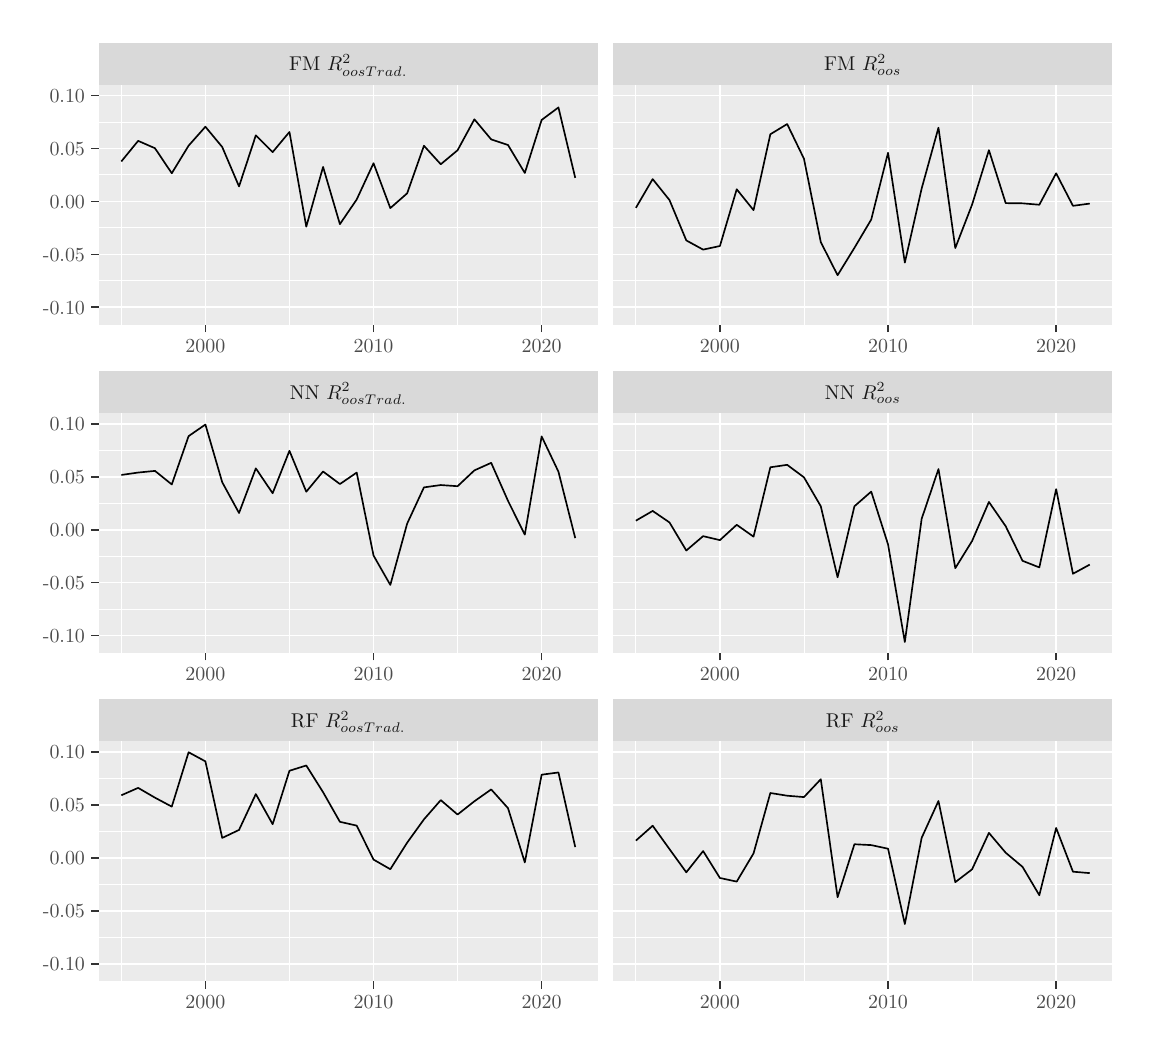
\begin{tikzpicture}[x=1pt,y=1pt]
\definecolor{fillColor}{RGB}{255,255,255}
\path[use as bounding box,fill=fillColor,fill opacity=0.00] (0,0) rectangle (397.48,361.35);
\begin{scope}
\path[clip] (  0.00,  0.00) rectangle (397.48,361.35);
\definecolor{drawColor}{RGB}{255,255,255}
\definecolor{fillColor}{RGB}{255,255,255}

\path[draw=drawColor,line width= 0.6pt,line join=round,line cap=round,fill=fillColor] (  0.00,  0.00) rectangle (397.48,361.35);
\end{scope}
\begin{scope}
\path[clip] ( 25.65,254.04) rectangle (206.07,340.69);
\definecolor{fillColor}{gray}{0.92}

\path[fill=fillColor] ( 25.65,254.04) rectangle (206.07,340.69);
\definecolor{drawColor}{RGB}{255,255,255}

\path[draw=drawColor,line width= 0.3pt,line join=round] ( 25.65,269.86) --
	(206.07,269.86);

\path[draw=drawColor,line width= 0.3pt,line join=round] ( 25.65,289.00) --
	(206.07,289.00);

\path[draw=drawColor,line width= 0.3pt,line join=round] ( 25.65,308.14) --
	(206.07,308.14);

\path[draw=drawColor,line width= 0.3pt,line join=round] ( 25.65,327.27) --
	(206.07,327.27);

\path[draw=drawColor,line width= 0.3pt,line join=round] ( 33.85,254.04) --
	( 33.85,340.69);

\path[draw=drawColor,line width= 0.3pt,line join=round] ( 94.59,254.04) --
	( 94.59,340.69);

\path[draw=drawColor,line width= 0.3pt,line join=round] (155.34,254.04) --
	(155.34,340.69);

\path[draw=drawColor,line width= 0.6pt,line join=round] ( 25.65,260.30) --
	(206.07,260.30);

\path[draw=drawColor,line width= 0.6pt,line join=round] ( 25.65,279.43) --
	(206.07,279.43);

\path[draw=drawColor,line width= 0.6pt,line join=round] ( 25.65,298.57) --
	(206.07,298.57);

\path[draw=drawColor,line width= 0.6pt,line join=round] ( 25.65,317.70) --
	(206.07,317.70);

\path[draw=drawColor,line width= 0.6pt,line join=round] ( 25.65,336.84) --
	(206.07,336.84);

\path[draw=drawColor,line width= 0.6pt,line join=round] ( 64.22,254.04) --
	( 64.22,340.69);

\path[draw=drawColor,line width= 0.6pt,line join=round] (124.97,254.04) --
	(124.97,340.69);

\path[draw=drawColor,line width= 0.6pt,line join=round] (185.72,254.04) --
	(185.72,340.69);
\definecolor{drawColor}{RGB}{0,0,0}

\path[draw=drawColor,line width= 0.6pt,line join=round] ( 33.85,313.01) --
	( 39.92,320.45) --
	( 46.00,317.78) --
	( 52.07,308.74) --
	( 58.15,318.71) --
	( 64.22,325.55) --
	( 70.30,318.22) --
	( 76.37,303.98) --
	( 82.44,322.44) --
	( 88.52,316.38) --
	( 94.59,323.66) --
	(100.67,289.44) --
	(106.74,311.03) --
	(112.82,290.35) --
	(118.89,299.26) --
	(124.97,312.36) --
	(131.04,296.15) --
	(137.12,301.48) --
	(143.19,318.67) --
	(149.27,311.99) --
	(155.34,317.05) --
	(161.42,328.23) --
	(167.49,320.97) --
	(173.57,318.94) --
	(179.64,308.84) --
	(185.72,328.01) --
	(191.79,332.52) --
	(197.86,307.08);
\end{scope}
\begin{scope}
\path[clip] ( 25.65,135.43) rectangle (206.07,222.07);
\definecolor{fillColor}{gray}{0.92}

\path[fill=fillColor] ( 25.65,135.43) rectangle (206.07,222.07);
\definecolor{drawColor}{RGB}{255,255,255}

\path[draw=drawColor,line width= 0.3pt,line join=round] ( 25.65,151.25) --
	(206.07,151.25);

\path[draw=drawColor,line width= 0.3pt,line join=round] ( 25.65,170.38) --
	(206.07,170.38);

\path[draw=drawColor,line width= 0.3pt,line join=round] ( 25.65,189.52) --
	(206.07,189.52);

\path[draw=drawColor,line width= 0.3pt,line join=round] ( 25.65,208.65) --
	(206.07,208.65);

\path[draw=drawColor,line width= 0.3pt,line join=round] ( 33.85,135.43) --
	( 33.85,222.07);

\path[draw=drawColor,line width= 0.3pt,line join=round] ( 94.59,135.43) --
	( 94.59,222.07);

\path[draw=drawColor,line width= 0.3pt,line join=round] (155.34,135.43) --
	(155.34,222.07);

\path[draw=drawColor,line width= 0.6pt,line join=round] ( 25.65,141.68) --
	(206.07,141.68);

\path[draw=drawColor,line width= 0.6pt,line join=round] ( 25.65,160.81) --
	(206.07,160.81);

\path[draw=drawColor,line width= 0.6pt,line join=round] ( 25.65,179.95) --
	(206.07,179.95);

\path[draw=drawColor,line width= 0.6pt,line join=round] ( 25.65,199.09) --
	(206.07,199.09);

\path[draw=drawColor,line width= 0.6pt,line join=round] ( 25.65,218.22) --
	(206.07,218.22);

\path[draw=drawColor,line width= 0.6pt,line join=round] ( 64.22,135.43) --
	( 64.22,222.07);

\path[draw=drawColor,line width= 0.6pt,line join=round] (124.97,135.43) --
	(124.97,222.07);

\path[draw=drawColor,line width= 0.6pt,line join=round] (185.72,135.43) --
	(185.72,222.07);
\definecolor{drawColor}{RGB}{0,0,0}

\path[draw=drawColor,line width= 0.6pt,line join=round] ( 33.85,199.72) --
	( 39.92,200.59) --
	( 46.00,201.19) --
	( 52.07,196.29) --
	( 58.15,213.75) --
	( 64.22,217.94) --
	( 70.30,197.08) --
	( 76.37,185.98) --
	( 82.44,202.10) --
	( 88.52,193.11) --
	( 94.59,208.45) --
	(100.67,193.67) --
	(106.74,200.98) --
	(112.82,196.43) --
	(118.89,200.58) --
	(124.97,170.61) --
	(131.04,159.98) --
	(137.12,182.13) --
	(143.19,195.23) --
	(149.27,196.08) --
	(155.34,195.65) --
	(161.42,201.38) --
	(167.49,204.10) --
	(173.57,190.35) --
	(179.64,178.17) --
	(185.72,213.65) --
	(191.79,200.90) --
	(197.86,176.91);
\end{scope}
\begin{scope}
\path[clip] ( 25.65, 16.81) rectangle (206.07,103.46);
\definecolor{fillColor}{gray}{0.92}

\path[fill=fillColor] ( 25.65, 16.81) rectangle (206.07,103.46);
\definecolor{drawColor}{RGB}{255,255,255}

\path[draw=drawColor,line width= 0.3pt,line join=round] ( 25.65, 32.63) --
	(206.07, 32.63);

\path[draw=drawColor,line width= 0.3pt,line join=round] ( 25.65, 51.77) --
	(206.07, 51.77);

\path[draw=drawColor,line width= 0.3pt,line join=round] ( 25.65, 70.90) --
	(206.07, 70.90);

\path[draw=drawColor,line width= 0.3pt,line join=round] ( 25.65, 90.04) --
	(206.07, 90.04);

\path[draw=drawColor,line width= 0.3pt,line join=round] ( 33.85, 16.81) --
	( 33.85,103.46);

\path[draw=drawColor,line width= 0.3pt,line join=round] ( 94.59, 16.81) --
	( 94.59,103.46);

\path[draw=drawColor,line width= 0.3pt,line join=round] (155.34, 16.81) --
	(155.34,103.46);

\path[draw=drawColor,line width= 0.6pt,line join=round] ( 25.65, 23.06) --
	(206.07, 23.06);

\path[draw=drawColor,line width= 0.6pt,line join=round] ( 25.65, 42.20) --
	(206.07, 42.20);

\path[draw=drawColor,line width= 0.6pt,line join=round] ( 25.65, 61.33) --
	(206.07, 61.33);

\path[draw=drawColor,line width= 0.6pt,line join=round] ( 25.65, 80.47) --
	(206.07, 80.47);

\path[draw=drawColor,line width= 0.6pt,line join=round] ( 25.65, 99.61) --
	(206.07, 99.61);

\path[draw=drawColor,line width= 0.6pt,line join=round] ( 64.22, 16.81) --
	( 64.22,103.46);

\path[draw=drawColor,line width= 0.6pt,line join=round] (124.97, 16.81) --
	(124.97,103.46);

\path[draw=drawColor,line width= 0.6pt,line join=round] (185.72, 16.81) --
	(185.72,103.46);
\definecolor{drawColor}{RGB}{0,0,0}

\path[draw=drawColor,line width= 0.6pt,line join=round] ( 33.85, 83.98) --
	( 39.92, 86.65) --
	( 46.00, 83.11) --
	( 52.07, 79.87) --
	( 58.15, 99.52) --
	( 64.22, 96.23) --
	( 70.30, 68.56) --
	( 76.37, 71.45) --
	( 82.44, 84.41) --
	( 88.52, 73.53) --
	( 94.59, 92.83) --
	(100.67, 94.74) --
	(106.74, 85.09) --
	(112.82, 74.39) --
	(118.89, 73.01) --
	(124.97, 60.74) --
	(131.04, 57.26) --
	(137.12, 66.85) --
	(143.19, 75.26) --
	(149.27, 82.23) --
	(155.34, 77.01) --
	(161.42, 81.81) --
	(167.49, 86.09) --
	(173.57, 79.31) --
	(179.64, 59.71) --
	(185.72, 91.41) --
	(191.79, 92.22) --
	(197.86, 65.26);
\end{scope}
\begin{scope}
\path[clip] (211.57,254.04) rectangle (391.98,340.69);
\definecolor{fillColor}{gray}{0.92}

\path[fill=fillColor] (211.57,254.04) rectangle (391.98,340.69);
\definecolor{drawColor}{RGB}{255,255,255}

\path[draw=drawColor,line width= 0.3pt,line join=round] (211.57,269.86) --
	(391.98,269.86);

\path[draw=drawColor,line width= 0.3pt,line join=round] (211.57,289.00) --
	(391.98,289.00);

\path[draw=drawColor,line width= 0.3pt,line join=round] (211.57,308.14) --
	(391.98,308.14);

\path[draw=drawColor,line width= 0.3pt,line join=round] (211.57,327.27) --
	(391.98,327.27);

\path[draw=drawColor,line width= 0.3pt,line join=round] (219.77,254.04) --
	(219.77,340.69);

\path[draw=drawColor,line width= 0.3pt,line join=round] (280.51,254.04) --
	(280.51,340.69);

\path[draw=drawColor,line width= 0.3pt,line join=round] (341.26,254.04) --
	(341.26,340.69);

\path[draw=drawColor,line width= 0.6pt,line join=round] (211.57,260.30) --
	(391.98,260.30);

\path[draw=drawColor,line width= 0.6pt,line join=round] (211.57,279.43) --
	(391.98,279.43);

\path[draw=drawColor,line width= 0.6pt,line join=round] (211.57,298.57) --
	(391.98,298.57);

\path[draw=drawColor,line width= 0.6pt,line join=round] (211.57,317.70) --
	(391.98,317.70);

\path[draw=drawColor,line width= 0.6pt,line join=round] (211.57,336.84) --
	(391.98,336.84);

\path[draw=drawColor,line width= 0.6pt,line join=round] (250.14,254.04) --
	(250.14,340.69);

\path[draw=drawColor,line width= 0.6pt,line join=round] (310.89,254.04) --
	(310.89,340.69);

\path[draw=drawColor,line width= 0.6pt,line join=round] (371.63,254.04) --
	(371.63,340.69);
\definecolor{drawColor}{RGB}{0,0,0}

\path[draw=drawColor,line width= 0.6pt,line join=round] (219.77,296.24) --
	(225.84,306.63) --
	(231.92,299.05) --
	(237.99,284.47) --
	(244.07,281.15) --
	(250.14,282.45) --
	(256.21,302.95) --
	(262.29,295.40) --
	(268.36,322.83) --
	(274.44,326.52) --
	(280.51,313.98) --
	(286.59,283.86) --
	(292.66,271.90) --
	(298.74,281.78) --
	(304.81,292.01) --
	(310.89,316.14) --
	(316.96,276.44) --
	(323.04,303.23) --
	(329.11,325.21) --
	(335.19,281.72) --
	(341.26,297.41) --
	(347.34,317.08) --
	(353.41,297.94) --
	(359.49,297.87) --
	(365.56,297.36) --
	(371.63,308.73) --
	(377.71,296.97) --
	(383.78,297.78);
\end{scope}
\begin{scope}
\path[clip] (211.57,135.43) rectangle (391.98,222.07);
\definecolor{fillColor}{gray}{0.92}

\path[fill=fillColor] (211.57,135.43) rectangle (391.98,222.07);
\definecolor{drawColor}{RGB}{255,255,255}

\path[draw=drawColor,line width= 0.3pt,line join=round] (211.57,151.25) --
	(391.98,151.25);

\path[draw=drawColor,line width= 0.3pt,line join=round] (211.57,170.38) --
	(391.98,170.38);

\path[draw=drawColor,line width= 0.3pt,line join=round] (211.57,189.52) --
	(391.98,189.52);

\path[draw=drawColor,line width= 0.3pt,line join=round] (211.57,208.65) --
	(391.98,208.65);

\path[draw=drawColor,line width= 0.3pt,line join=round] (219.77,135.43) --
	(219.77,222.07);

\path[draw=drawColor,line width= 0.3pt,line join=round] (280.51,135.43) --
	(280.51,222.07);

\path[draw=drawColor,line width= 0.3pt,line join=round] (341.26,135.43) --
	(341.26,222.07);

\path[draw=drawColor,line width= 0.6pt,line join=round] (211.57,141.68) --
	(391.98,141.68);

\path[draw=drawColor,line width= 0.6pt,line join=round] (211.57,160.81) --
	(391.98,160.81);

\path[draw=drawColor,line width= 0.6pt,line join=round] (211.57,179.95) --
	(391.98,179.95);

\path[draw=drawColor,line width= 0.6pt,line join=round] (211.57,199.09) --
	(391.98,199.09);

\path[draw=drawColor,line width= 0.6pt,line join=round] (211.57,218.22) --
	(391.98,218.22);

\path[draw=drawColor,line width= 0.6pt,line join=round] (250.14,135.43) --
	(250.14,222.07);

\path[draw=drawColor,line width= 0.6pt,line join=round] (310.89,135.43) --
	(310.89,222.07);

\path[draw=drawColor,line width= 0.6pt,line join=round] (371.63,135.43) --
	(371.63,222.07);
\definecolor{drawColor}{RGB}{0,0,0}

\path[draw=drawColor,line width= 0.6pt,line join=round] (219.77,183.20) --
	(225.84,186.72) --
	(231.92,182.56) --
	(237.99,172.42) --
	(244.07,177.61) --
	(250.14,176.17) --
	(256.21,181.71) --
	(262.29,177.42) --
	(268.36,202.49) --
	(274.44,203.38) --
	(280.51,198.86) --
	(286.59,188.41) --
	(292.66,162.75) --
	(298.74,188.40) --
	(304.81,193.71) --
	(310.89,174.63) --
	(316.96,139.36) --
	(323.04,183.88) --
	(329.11,201.85) --
	(335.19,166.04) --
	(341.26,175.86) --
	(347.34,189.97) --
	(353.41,181.18) --
	(359.49,168.70) --
	(365.56,166.31) --
	(371.63,194.61) --
	(377.71,164.02) --
	(383.78,167.33);
\end{scope}
\begin{scope}
\path[clip] (211.57, 16.81) rectangle (391.98,103.46);
\definecolor{fillColor}{gray}{0.92}

\path[fill=fillColor] (211.57, 16.81) rectangle (391.98,103.46);
\definecolor{drawColor}{RGB}{255,255,255}

\path[draw=drawColor,line width= 0.3pt,line join=round] (211.57, 32.63) --
	(391.98, 32.63);

\path[draw=drawColor,line width= 0.3pt,line join=round] (211.57, 51.77) --
	(391.98, 51.77);

\path[draw=drawColor,line width= 0.3pt,line join=round] (211.57, 70.90) --
	(391.98, 70.90);

\path[draw=drawColor,line width= 0.3pt,line join=round] (211.57, 90.04) --
	(391.98, 90.04);

\path[draw=drawColor,line width= 0.3pt,line join=round] (219.77, 16.81) --
	(219.77,103.46);

\path[draw=drawColor,line width= 0.3pt,line join=round] (280.51, 16.81) --
	(280.51,103.46);

\path[draw=drawColor,line width= 0.3pt,line join=round] (341.26, 16.81) --
	(341.26,103.46);

\path[draw=drawColor,line width= 0.6pt,line join=round] (211.57, 23.06) --
	(391.98, 23.06);

\path[draw=drawColor,line width= 0.6pt,line join=round] (211.57, 42.20) --
	(391.98, 42.20);

\path[draw=drawColor,line width= 0.6pt,line join=round] (211.57, 61.33) --
	(391.98, 61.33);

\path[draw=drawColor,line width= 0.6pt,line join=round] (211.57, 80.47) --
	(391.98, 80.47);

\path[draw=drawColor,line width= 0.6pt,line join=round] (211.57, 99.61) --
	(391.98, 99.61);

\path[draw=drawColor,line width= 0.6pt,line join=round] (250.14, 16.81) --
	(250.14,103.46);

\path[draw=drawColor,line width= 0.6pt,line join=round] (310.89, 16.81) --
	(310.89,103.46);

\path[draw=drawColor,line width= 0.6pt,line join=round] (371.63, 16.81) --
	(371.63,103.46);
\definecolor{drawColor}{RGB}{0,0,0}

\path[draw=drawColor,line width= 0.6pt,line join=round] (219.77, 67.59) --
	(225.84, 72.96) --
	(231.92, 64.52) --
	(237.99, 56.14) --
	(244.07, 63.82) --
	(250.14, 54.09) --
	(256.21, 52.78) --
	(262.29, 62.98) --
	(268.36, 84.80) --
	(274.44, 83.82) --
	(280.51, 83.32) --
	(286.59, 89.77) --
	(292.66, 47.15) --
	(298.74, 66.28) --
	(304.81, 65.97) --
	(310.89, 64.67) --
	(316.96, 37.46) --
	(323.04, 68.60) --
	(329.11, 81.92) --
	(335.19, 52.58) --
	(341.26, 57.22) --
	(347.34, 70.38) --
	(353.41, 63.21) --
	(359.49, 58.11) --
	(365.56, 47.86) --
	(371.63, 72.17) --
	(377.71, 56.36) --
	(383.78, 55.85);
\end{scope}
\begin{scope}
\path[clip] ( 25.65,103.46) rectangle (206.07,118.62);
\definecolor{fillColor}{gray}{0.85}

\path[fill=fillColor] ( 25.65,103.46) rectangle (206.07,118.62);
\definecolor{drawColor}{gray}{0.10}

\node[text=drawColor,anchor=base,inner sep=0pt, outer sep=0pt, scale=  0.72] at (115.86,108.56) {RF $R^2_{oos  Trad.}$};
\end{scope}
\begin{scope}
\path[clip] (211.57,103.46) rectangle (391.98,118.62);
\definecolor{fillColor}{gray}{0.85}

\path[fill=fillColor] (211.57,103.46) rectangle (391.98,118.62);
\definecolor{drawColor}{gray}{0.10}

\node[text=drawColor,anchor=base,inner sep=0pt, outer sep=0pt, scale=  0.72] at (301.78,108.56) {RF $R^2_{oos}$};
\end{scope}
\begin{scope}
\path[clip] ( 25.65,222.07) rectangle (206.07,237.23);
\definecolor{fillColor}{gray}{0.85}

\path[fill=fillColor] ( 25.65,222.07) rectangle (206.07,237.23);
\definecolor{drawColor}{gray}{0.10}

\node[text=drawColor,anchor=base,inner sep=0pt, outer sep=0pt, scale=  0.72] at (115.86,227.17) {NN $R^2_{oos  Trad.}$};
\end{scope}
\begin{scope}
\path[clip] (211.57,222.07) rectangle (391.98,237.23);
\definecolor{fillColor}{gray}{0.85}

\path[fill=fillColor] (211.57,222.07) rectangle (391.98,237.23);
\definecolor{drawColor}{gray}{0.10}

\node[text=drawColor,anchor=base,inner sep=0pt, outer sep=0pt, scale=  0.72] at (301.78,227.17) {NN $R^2_{oos}$};
\end{scope}
\begin{scope}
\path[clip] ( 25.65,340.69) rectangle (206.07,355.85);
\definecolor{fillColor}{gray}{0.85}

\path[fill=fillColor] ( 25.65,340.69) rectangle (206.07,355.85);
\definecolor{drawColor}{gray}{0.10}

\node[text=drawColor,anchor=base,inner sep=0pt, outer sep=0pt, scale=  0.72] at (115.86,345.79) {FM $R^2_{oos  Trad.}$};
\end{scope}
\begin{scope}
\path[clip] (211.57,340.69) rectangle (391.98,355.85);
\definecolor{fillColor}{gray}{0.85}

\path[fill=fillColor] (211.57,340.69) rectangle (391.98,355.85);
\definecolor{drawColor}{gray}{0.10}

\node[text=drawColor,anchor=base,inner sep=0pt, outer sep=0pt, scale=  0.72] at (301.78,345.79) {FM $R^2_{oos}$};
\end{scope}
\begin{scope}
\path[clip] (  0.00,  0.00) rectangle (397.48,361.35);
\definecolor{drawColor}{gray}{0.20}

\path[draw=drawColor,line width= 0.6pt,line join=round] ( 64.22, 14.06) --
	( 64.22, 16.81);

\path[draw=drawColor,line width= 0.6pt,line join=round] (124.97, 14.06) --
	(124.97, 16.81);

\path[draw=drawColor,line width= 0.6pt,line join=round] (185.72, 14.06) --
	(185.72, 16.81);
\end{scope}
\begin{scope}
\path[clip] (  0.00,  0.00) rectangle (397.48,361.35);
\definecolor{drawColor}{gray}{0.30}

\node[text=drawColor,anchor=base,inner sep=0pt, outer sep=0pt, scale=  0.72] at ( 64.22,  6.90) {2000};

\node[text=drawColor,anchor=base,inner sep=0pt, outer sep=0pt, scale=  0.72] at (124.97,  6.90) {2010};

\node[text=drawColor,anchor=base,inner sep=0pt, outer sep=0pt, scale=  0.72] at (185.72,  6.90) {2020};
\end{scope}
\begin{scope}
\path[clip] (  0.00,  0.00) rectangle (397.48,361.35);
\definecolor{drawColor}{gray}{0.20}

\path[draw=drawColor,line width= 0.6pt,line join=round] (250.14, 14.06) --
	(250.14, 16.81);

\path[draw=drawColor,line width= 0.6pt,line join=round] (310.89, 14.06) --
	(310.89, 16.81);

\path[draw=drawColor,line width= 0.6pt,line join=round] (371.63, 14.06) --
	(371.63, 16.81);
\end{scope}
\begin{scope}
\path[clip] (  0.00,  0.00) rectangle (397.48,361.35);
\definecolor{drawColor}{gray}{0.30}

\node[text=drawColor,anchor=base,inner sep=0pt, outer sep=0pt, scale=  0.72] at (250.14,  6.90) {2000};

\node[text=drawColor,anchor=base,inner sep=0pt, outer sep=0pt, scale=  0.72] at (310.89,  6.90) {2010};

\node[text=drawColor,anchor=base,inner sep=0pt, outer sep=0pt, scale=  0.72] at (371.63,  6.90) {2020};
\end{scope}
\begin{scope}
\path[clip] (  0.00,  0.00) rectangle (397.48,361.35);
\definecolor{drawColor}{gray}{0.20}

\path[draw=drawColor,line width= 0.6pt,line join=round] ( 64.22,132.68) --
	( 64.22,135.43);

\path[draw=drawColor,line width= 0.6pt,line join=round] (124.97,132.68) --
	(124.97,135.43);

\path[draw=drawColor,line width= 0.6pt,line join=round] (185.72,132.68) --
	(185.72,135.43);
\end{scope}
\begin{scope}
\path[clip] (  0.00,  0.00) rectangle (397.48,361.35);
\definecolor{drawColor}{gray}{0.30}

\node[text=drawColor,anchor=base,inner sep=0pt, outer sep=0pt, scale=  0.72] at ( 64.22,125.52) {2000};

\node[text=drawColor,anchor=base,inner sep=0pt, outer sep=0pt, scale=  0.72] at (124.97,125.52) {2010};

\node[text=drawColor,anchor=base,inner sep=0pt, outer sep=0pt, scale=  0.72] at (185.72,125.52) {2020};
\end{scope}
\begin{scope}
\path[clip] (  0.00,  0.00) rectangle (397.48,361.35);
\definecolor{drawColor}{gray}{0.20}

\path[draw=drawColor,line width= 0.6pt,line join=round] (250.14,132.68) --
	(250.14,135.43);

\path[draw=drawColor,line width= 0.6pt,line join=round] (310.89,132.68) --
	(310.89,135.43);

\path[draw=drawColor,line width= 0.6pt,line join=round] (371.63,132.68) --
	(371.63,135.43);
\end{scope}
\begin{scope}
\path[clip] (  0.00,  0.00) rectangle (397.48,361.35);
\definecolor{drawColor}{gray}{0.30}

\node[text=drawColor,anchor=base,inner sep=0pt, outer sep=0pt, scale=  0.72] at (250.14,125.52) {2000};

\node[text=drawColor,anchor=base,inner sep=0pt, outer sep=0pt, scale=  0.72] at (310.89,125.52) {2010};

\node[text=drawColor,anchor=base,inner sep=0pt, outer sep=0pt, scale=  0.72] at (371.63,125.52) {2020};
\end{scope}
\begin{scope}
\path[clip] (  0.00,  0.00) rectangle (397.48,361.35);
\definecolor{drawColor}{gray}{0.20}

\path[draw=drawColor,line width= 0.6pt,line join=round] ( 64.22,251.29) --
	( 64.22,254.04);

\path[draw=drawColor,line width= 0.6pt,line join=round] (124.97,251.29) --
	(124.97,254.04);

\path[draw=drawColor,line width= 0.6pt,line join=round] (185.72,251.29) --
	(185.72,254.04);
\end{scope}
\begin{scope}
\path[clip] (  0.00,  0.00) rectangle (397.48,361.35);
\definecolor{drawColor}{gray}{0.30}

\node[text=drawColor,anchor=base,inner sep=0pt, outer sep=0pt, scale=  0.72] at ( 64.22,244.13) {2000};

\node[text=drawColor,anchor=base,inner sep=0pt, outer sep=0pt, scale=  0.72] at (124.97,244.13) {2010};

\node[text=drawColor,anchor=base,inner sep=0pt, outer sep=0pt, scale=  0.72] at (185.72,244.13) {2020};
\end{scope}
\begin{scope}
\path[clip] (  0.00,  0.00) rectangle (397.48,361.35);
\definecolor{drawColor}{gray}{0.20}

\path[draw=drawColor,line width= 0.6pt,line join=round] (250.14,251.29) --
	(250.14,254.04);

\path[draw=drawColor,line width= 0.6pt,line join=round] (310.89,251.29) --
	(310.89,254.04);

\path[draw=drawColor,line width= 0.6pt,line join=round] (371.63,251.29) --
	(371.63,254.04);
\end{scope}
\begin{scope}
\path[clip] (  0.00,  0.00) rectangle (397.48,361.35);
\definecolor{drawColor}{gray}{0.30}

\node[text=drawColor,anchor=base,inner sep=0pt, outer sep=0pt, scale=  0.72] at (250.14,244.13) {2000};

\node[text=drawColor,anchor=base,inner sep=0pt, outer sep=0pt, scale=  0.72] at (310.89,244.13) {2010};

\node[text=drawColor,anchor=base,inner sep=0pt, outer sep=0pt, scale=  0.72] at (371.63,244.13) {2020};
\end{scope}
\begin{scope}
\path[clip] (  0.00,  0.00) rectangle (397.48,361.35);
\definecolor{drawColor}{gray}{0.30}

\node[text=drawColor,anchor=base east,inner sep=0pt, outer sep=0pt, scale=  0.72] at ( 20.70,257.82) {-0.10};

\node[text=drawColor,anchor=base east,inner sep=0pt, outer sep=0pt, scale=  0.72] at ( 20.70,276.95) {-0.05};

\node[text=drawColor,anchor=base east,inner sep=0pt, outer sep=0pt, scale=  0.72] at ( 20.70,296.09) {0.00};

\node[text=drawColor,anchor=base east,inner sep=0pt, outer sep=0pt, scale=  0.72] at ( 20.70,315.22) {0.05};

\node[text=drawColor,anchor=base east,inner sep=0pt, outer sep=0pt, scale=  0.72] at ( 20.70,334.36) {0.10};
\end{scope}
\begin{scope}
\path[clip] (  0.00,  0.00) rectangle (397.48,361.35);
\definecolor{drawColor}{gray}{0.20}

\path[draw=drawColor,line width= 0.6pt,line join=round] ( 22.90,260.30) --
	( 25.65,260.30);

\path[draw=drawColor,line width= 0.6pt,line join=round] ( 22.90,279.43) --
	( 25.65,279.43);

\path[draw=drawColor,line width= 0.6pt,line join=round] ( 22.90,298.57) --
	( 25.65,298.57);

\path[draw=drawColor,line width= 0.6pt,line join=round] ( 22.90,317.70) --
	( 25.65,317.70);

\path[draw=drawColor,line width= 0.6pt,line join=round] ( 22.90,336.84) --
	( 25.65,336.84);
\end{scope}
\begin{scope}
\path[clip] (  0.00,  0.00) rectangle (397.48,361.35);
\definecolor{drawColor}{gray}{0.30}

\node[text=drawColor,anchor=base east,inner sep=0pt, outer sep=0pt, scale=  0.72] at ( 20.70,139.20) {-0.10};

\node[text=drawColor,anchor=base east,inner sep=0pt, outer sep=0pt, scale=  0.72] at ( 20.70,158.34) {-0.05};

\node[text=drawColor,anchor=base east,inner sep=0pt, outer sep=0pt, scale=  0.72] at ( 20.70,177.47) {0.00};

\node[text=drawColor,anchor=base east,inner sep=0pt, outer sep=0pt, scale=  0.72] at ( 20.70,196.61) {0.05};

\node[text=drawColor,anchor=base east,inner sep=0pt, outer sep=0pt, scale=  0.72] at ( 20.70,215.74) {0.10};
\end{scope}
\begin{scope}
\path[clip] (  0.00,  0.00) rectangle (397.48,361.35);
\definecolor{drawColor}{gray}{0.20}

\path[draw=drawColor,line width= 0.6pt,line join=round] ( 22.90,141.68) --
	( 25.65,141.68);

\path[draw=drawColor,line width= 0.6pt,line join=round] ( 22.90,160.81) --
	( 25.65,160.81);

\path[draw=drawColor,line width= 0.6pt,line join=round] ( 22.90,179.95) --
	( 25.65,179.95);

\path[draw=drawColor,line width= 0.6pt,line join=round] ( 22.90,199.09) --
	( 25.65,199.09);

\path[draw=drawColor,line width= 0.6pt,line join=round] ( 22.90,218.22) --
	( 25.65,218.22);
\end{scope}
\begin{scope}
\path[clip] (  0.00,  0.00) rectangle (397.48,361.35);
\definecolor{drawColor}{gray}{0.30}

\node[text=drawColor,anchor=base east,inner sep=0pt, outer sep=0pt, scale=  0.72] at ( 20.70, 20.58) {-0.10};

\node[text=drawColor,anchor=base east,inner sep=0pt, outer sep=0pt, scale=  0.72] at ( 20.70, 39.72) {-0.05};

\node[text=drawColor,anchor=base east,inner sep=0pt, outer sep=0pt, scale=  0.72] at ( 20.70, 58.85) {0.00};

\node[text=drawColor,anchor=base east,inner sep=0pt, outer sep=0pt, scale=  0.72] at ( 20.70, 77.99) {0.05};

\node[text=drawColor,anchor=base east,inner sep=0pt, outer sep=0pt, scale=  0.72] at ( 20.70, 97.13) {0.10};
\end{scope}
\begin{scope}
\path[clip] (  0.00,  0.00) rectangle (397.48,361.35);
\definecolor{drawColor}{gray}{0.20}

\path[draw=drawColor,line width= 0.6pt,line join=round] ( 22.90, 23.06) --
	( 25.65, 23.06);

\path[draw=drawColor,line width= 0.6pt,line join=round] ( 22.90, 42.20) --
	( 25.65, 42.20);

\path[draw=drawColor,line width= 0.6pt,line join=round] ( 22.90, 61.33) --
	( 25.65, 61.33);

\path[draw=drawColor,line width= 0.6pt,line join=round] ( 22.90, 80.47) --
	( 25.65, 80.47);

\path[draw=drawColor,line width= 0.6pt,line join=round] ( 22.90, 99.61) --
	( 25.65, 99.61);
\end{scope}
\end{tikzpicture}

\label{plot:OOSR2_ts}
\end{figure}

\begin{figure}[H]
\centering
\caption[Turnover of long-short machine learning portfolios]{\textbf{Turnover of long-short machine learning portfolios \textnormal{- Own source}}\\ Figure plots time series of turnover of the long-short portfolios. Values shown are mean turnovers of prediction periods. FM stands for linear regression model, RF stands for random forest model and NN stands for neural networks model. }
% Created by tikzDevice version 0.12.6 on 2024-03-11 18:45:03
% !TEX encoding = UTF-8 Unicode
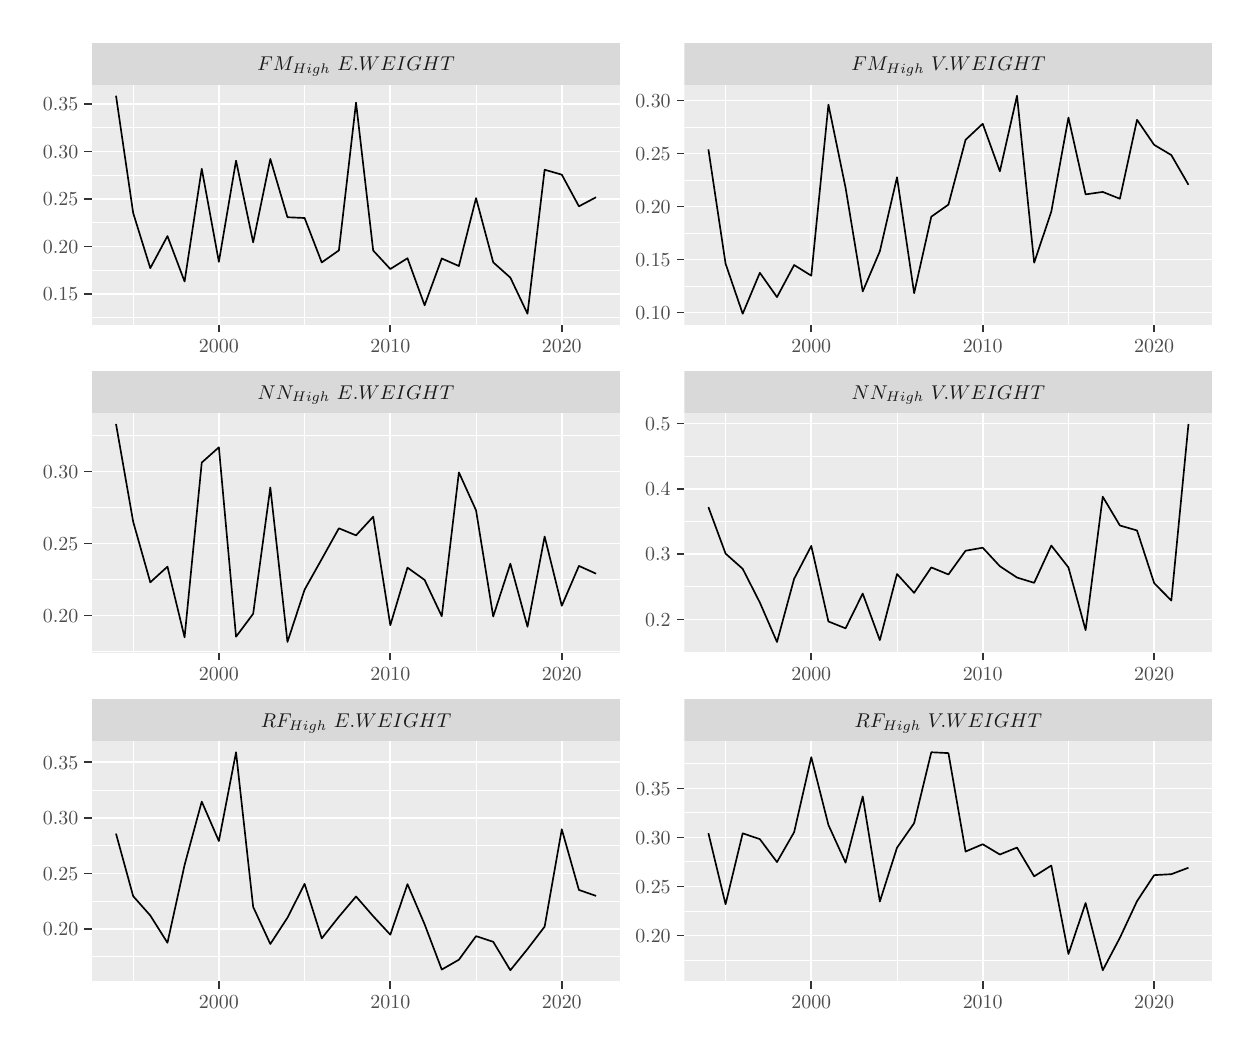
\begin{tikzpicture}[x=1pt,y=1pt]
\definecolor{fillColor}{RGB}{255,255,255}
\path[use as bounding box,fill=fillColor,fill opacity=0.00] (0,0) rectangle (433.62,361.35);
\begin{scope}
\path[clip] (  0.00,  0.00) rectangle (433.62,361.35);
\definecolor{drawColor}{RGB}{255,255,255}
\definecolor{fillColor}{RGB}{255,255,255}

\path[draw=drawColor,line width= 0.6pt,line join=round,line cap=round,fill=fillColor] (  0.00,  0.00) rectangle (433.62,361.35);
\end{scope}
\begin{scope}
\path[clip] ( 23.25,254.04) rectangle (214.06,340.69);
\definecolor{fillColor}{gray}{0.92}

\path[fill=fillColor] ( 23.25,254.04) rectangle (214.06,340.69);
\definecolor{drawColor}{RGB}{255,255,255}

\path[draw=drawColor,line width= 0.3pt,line join=round] ( 23.25,256.50) --
	(214.06,256.50);

\path[draw=drawColor,line width= 0.3pt,line join=round] ( 23.25,273.67) --
	(214.06,273.67);

\path[draw=drawColor,line width= 0.3pt,line join=round] ( 23.25,290.84) --
	(214.06,290.84);

\path[draw=drawColor,line width= 0.3pt,line join=round] ( 23.25,308.01) --
	(214.06,308.01);

\path[draw=drawColor,line width= 0.3pt,line join=round] ( 23.25,325.18) --
	(214.06,325.18);

\path[draw=drawColor,line width= 0.3pt,line join=round] ( 38.12,254.04) --
	( 38.12,340.69);

\path[draw=drawColor,line width= 0.3pt,line join=round] (100.07,254.04) --
	(100.07,340.69);

\path[draw=drawColor,line width= 0.3pt,line join=round] (162.02,254.04) --
	(162.02,340.69);

\path[draw=drawColor,line width= 0.6pt,line join=round] ( 23.25,265.09) --
	(214.06,265.09);

\path[draw=drawColor,line width= 0.6pt,line join=round] ( 23.25,282.26) --
	(214.06,282.26);

\path[draw=drawColor,line width= 0.6pt,line join=round] ( 23.25,299.43) --
	(214.06,299.43);

\path[draw=drawColor,line width= 0.6pt,line join=round] ( 23.25,316.60) --
	(214.06,316.60);

\path[draw=drawColor,line width= 0.6pt,line join=round] ( 23.25,333.77) --
	(214.06,333.77);

\path[draw=drawColor,line width= 0.6pt,line join=round] ( 69.09,254.04) --
	( 69.09,340.69);

\path[draw=drawColor,line width= 0.6pt,line join=round] (131.04,254.04) --
	(131.04,340.69);

\path[draw=drawColor,line width= 0.6pt,line join=round] (193.00,254.04) --
	(193.00,340.69);
\definecolor{drawColor}{RGB}{0,0,0}

\path[draw=drawColor,line width= 0.6pt,line join=round] ( 31.92,336.75) --
	( 38.12,294.39) --
	( 44.31,274.45) --
	( 50.51,286.04) --
	( 56.70,269.63) --
	( 62.90,310.37) --
	( 69.09,276.73) --
	( 75.29,313.29) --
	( 81.48,283.78) --
	( 87.68,313.91) --
	( 93.87,292.85) --
	(100.07,292.57) --
	(106.26,276.51) --
	(112.46,280.87) --
	(118.65,334.26) --
	(124.85,280.82) --
	(131.04,274.13) --
	(137.24,278.03) --
	(143.43,261.03) --
	(149.63,277.94) --
	(155.82,275.22) --
	(162.02,299.75) --
	(168.22,276.55) --
	(174.41,271.03) --
	(180.61,257.98) --
	(186.80,310.01) --
	(193.00,308.24) --
	(199.19,296.79) --
	(205.39,300.07);
\end{scope}
\begin{scope}
\path[clip] ( 23.25,135.43) rectangle (214.06,222.07);
\definecolor{fillColor}{gray}{0.92}

\path[fill=fillColor] ( 23.25,135.43) rectangle (214.06,222.07);
\definecolor{drawColor}{RGB}{255,255,255}

\path[draw=drawColor,line width= 0.3pt,line join=round] ( 23.25,135.94) --
	(214.06,135.94);

\path[draw=drawColor,line width= 0.3pt,line join=round] ( 23.25,161.96) --
	(214.06,161.96);

\path[draw=drawColor,line width= 0.3pt,line join=round] ( 23.25,187.98) --
	(214.06,187.98);

\path[draw=drawColor,line width= 0.3pt,line join=round] ( 23.25,214.00) --
	(214.06,214.00);

\path[draw=drawColor,line width= 0.3pt,line join=round] ( 38.12,135.43) --
	( 38.12,222.07);

\path[draw=drawColor,line width= 0.3pt,line join=round] (100.07,135.43) --
	(100.07,222.07);

\path[draw=drawColor,line width= 0.3pt,line join=round] (162.02,135.43) --
	(162.02,222.07);

\path[draw=drawColor,line width= 0.6pt,line join=round] ( 23.25,148.95) --
	(214.06,148.95);

\path[draw=drawColor,line width= 0.6pt,line join=round] ( 23.25,174.97) --
	(214.06,174.97);

\path[draw=drawColor,line width= 0.6pt,line join=round] ( 23.25,200.99) --
	(214.06,200.99);

\path[draw=drawColor,line width= 0.6pt,line join=round] ( 69.09,135.43) --
	( 69.09,222.07);

\path[draw=drawColor,line width= 0.6pt,line join=round] (131.04,135.43) --
	(131.04,222.07);

\path[draw=drawColor,line width= 0.6pt,line join=round] (193.00,135.43) --
	(193.00,222.07);
\definecolor{drawColor}{RGB}{0,0,0}

\path[draw=drawColor,line width= 0.6pt,line join=round] ( 31.92,218.14) --
	( 38.12,182.84) --
	( 44.31,160.94) --
	( 50.51,166.59) --
	( 56.70,141.06) --
	( 62.90,204.19) --
	( 69.09,209.72) --
	( 75.29,141.28) --
	( 81.48,149.55) --
	( 87.68,195.19) --
	( 93.87,139.36) --
	(100.07,158.28) --
	(106.26,169.32) --
	(112.46,180.45) --
	(118.65,177.89) --
	(124.85,184.63) --
	(131.04,145.43) --
	(137.24,166.23) --
	(143.43,161.79) --
	(149.63,148.67) --
	(155.82,200.65) --
	(162.02,186.92) --
	(168.22,148.57) --
	(174.41,167.65) --
	(180.61,144.88) --
	(186.80,177.47) --
	(193.00,152.44) --
	(199.19,166.85) --
	(205.39,164.05);
\end{scope}
\begin{scope}
\path[clip] ( 23.25, 16.81) rectangle (214.06,103.46);
\definecolor{fillColor}{gray}{0.92}

\path[fill=fillColor] ( 23.25, 16.81) rectangle (214.06,103.46);
\definecolor{drawColor}{RGB}{255,255,255}

\path[draw=drawColor,line width= 0.3pt,line join=round] ( 23.25, 25.58) --
	(214.06, 25.58);

\path[draw=drawColor,line width= 0.3pt,line join=round] ( 23.25, 45.68) --
	(214.06, 45.68);

\path[draw=drawColor,line width= 0.3pt,line join=round] ( 23.25, 65.79) --
	(214.06, 65.79);

\path[draw=drawColor,line width= 0.3pt,line join=round] ( 23.25, 85.89) --
	(214.06, 85.89);

\path[draw=drawColor,line width= 0.3pt,line join=round] ( 38.12, 16.81) --
	( 38.12,103.46);

\path[draw=drawColor,line width= 0.3pt,line join=round] (100.07, 16.81) --
	(100.07,103.46);

\path[draw=drawColor,line width= 0.3pt,line join=round] (162.02, 16.81) --
	(162.02,103.46);

\path[draw=drawColor,line width= 0.6pt,line join=round] ( 23.25, 35.63) --
	(214.06, 35.63);

\path[draw=drawColor,line width= 0.6pt,line join=round] ( 23.25, 55.74) --
	(214.06, 55.74);

\path[draw=drawColor,line width= 0.6pt,line join=round] ( 23.25, 75.84) --
	(214.06, 75.84);

\path[draw=drawColor,line width= 0.6pt,line join=round] ( 23.25, 95.95) --
	(214.06, 95.95);

\path[draw=drawColor,line width= 0.6pt,line join=round] ( 69.09, 16.81) --
	( 69.09,103.46);

\path[draw=drawColor,line width= 0.6pt,line join=round] (131.04, 16.81) --
	(131.04,103.46);

\path[draw=drawColor,line width= 0.6pt,line join=round] (193.00, 16.81) --
	(193.00,103.46);
\definecolor{drawColor}{RGB}{0,0,0}

\path[draw=drawColor,line width= 0.6pt,line join=round] ( 31.92, 70.11) --
	( 38.12, 47.52) --
	( 44.31, 40.53) --
	( 50.51, 30.68) --
	( 56.70, 58.79) --
	( 62.90, 81.69) --
	( 69.09, 67.43) --
	( 75.29, 99.52) --
	( 81.48, 43.63) --
	( 87.68, 30.23) --
	( 93.87, 39.73) --
	(100.07, 51.96) --
	(106.26, 32.26) --
	(112.46, 40.08) --
	(118.65, 47.41) --
	(124.85, 40.28) --
	(131.04, 33.60) --
	(137.24, 51.86) --
	(143.43, 37.36) --
	(149.63, 21.00) --
	(155.82, 24.55) --
	(162.02, 33.07) --
	(168.22, 31.04) --
	(174.41, 20.75) --
	(180.61, 28.41) --
	(186.80, 36.51) --
	(193.00, 71.68) --
	(199.19, 49.78) --
	(205.39, 47.61);
\end{scope}
\begin{scope}
\path[clip] (237.31,254.04) rectangle (428.12,340.69);
\definecolor{fillColor}{gray}{0.92}

\path[fill=fillColor] (237.31,254.04) rectangle (428.12,340.69);
\definecolor{drawColor}{RGB}{255,255,255}

\path[draw=drawColor,line width= 0.3pt,line join=round] (237.31,267.96) --
	(428.12,267.96);

\path[draw=drawColor,line width= 0.3pt,line join=round] (237.31,287.11) --
	(428.12,287.11);

\path[draw=drawColor,line width= 0.3pt,line join=round] (237.31,306.27) --
	(428.12,306.27);

\path[draw=drawColor,line width= 0.3pt,line join=round] (237.31,325.43) --
	(428.12,325.43);

\path[draw=drawColor,line width= 0.3pt,line join=round] (252.18,254.04) --
	(252.18,340.69);

\path[draw=drawColor,line width= 0.3pt,line join=round] (314.13,254.04) --
	(314.13,340.69);

\path[draw=drawColor,line width= 0.3pt,line join=round] (376.08,254.04) --
	(376.08,340.69);

\path[draw=drawColor,line width= 0.6pt,line join=round] (237.31,258.38) --
	(428.12,258.38);

\path[draw=drawColor,line width= 0.6pt,line join=round] (237.31,277.53) --
	(428.12,277.53);

\path[draw=drawColor,line width= 0.6pt,line join=round] (237.31,296.69) --
	(428.12,296.69);

\path[draw=drawColor,line width= 0.6pt,line join=round] (237.31,315.85) --
	(428.12,315.85);

\path[draw=drawColor,line width= 0.6pt,line join=round] (237.31,335.01) --
	(428.12,335.01);

\path[draw=drawColor,line width= 0.6pt,line join=round] (283.15,254.04) --
	(283.15,340.69);

\path[draw=drawColor,line width= 0.6pt,line join=round] (345.10,254.04) --
	(345.10,340.69);

\path[draw=drawColor,line width= 0.6pt,line join=round] (407.06,254.04) --
	(407.06,340.69);
\definecolor{drawColor}{RGB}{0,0,0}

\path[draw=drawColor,line width= 0.6pt,line join=round] (245.98,317.36) --
	(252.18,276.08) --
	(258.37,257.98) --
	(264.57,272.78) --
	(270.76,263.99) --
	(276.96,275.58) --
	(283.15,271.73) --
	(289.35,333.54) --
	(295.54,303.51) --
	(301.74,266.03) --
	(307.93,280.56) --
	(314.13,307.29) --
	(320.32,265.40) --
	(326.52,293.04) --
	(332.71,297.41) --
	(338.91,320.83) --
	(345.10,326.62) --
	(351.30,309.44) --
	(357.49,336.75) --
	(363.69,276.42) --
	(369.88,294.86) --
	(376.08,328.86) --
	(382.28,301.11) --
	(388.47,301.99) --
	(394.67,299.53) --
	(400.86,328.05) --
	(407.06,318.99) --
	(413.25,315.31) --
	(419.45,304.57);
\end{scope}
\begin{scope}
\path[clip] (237.31,135.43) rectangle (428.12,222.07);
\definecolor{fillColor}{gray}{0.92}

\path[fill=fillColor] (237.31,135.43) rectangle (428.12,222.07);
\definecolor{drawColor}{RGB}{255,255,255}

\path[draw=drawColor,line width= 0.3pt,line join=round] (237.31,135.76) --
	(428.12,135.76);

\path[draw=drawColor,line width= 0.3pt,line join=round] (237.31,159.34) --
	(428.12,159.34);

\path[draw=drawColor,line width= 0.3pt,line join=round] (237.31,182.91) --
	(428.12,182.91);

\path[draw=drawColor,line width= 0.3pt,line join=round] (237.31,206.49) --
	(428.12,206.49);

\path[draw=drawColor,line width= 0.3pt,line join=round] (252.18,135.43) --
	(252.18,222.07);

\path[draw=drawColor,line width= 0.3pt,line join=round] (314.13,135.43) --
	(314.13,222.07);

\path[draw=drawColor,line width= 0.3pt,line join=round] (376.08,135.43) --
	(376.08,222.07);

\path[draw=drawColor,line width= 0.6pt,line join=round] (237.31,147.55) --
	(428.12,147.55);

\path[draw=drawColor,line width= 0.6pt,line join=round] (237.31,171.12) --
	(428.12,171.12);

\path[draw=drawColor,line width= 0.6pt,line join=round] (237.31,194.70) --
	(428.12,194.70);

\path[draw=drawColor,line width= 0.6pt,line join=round] (237.31,218.28) --
	(428.12,218.28);

\path[draw=drawColor,line width= 0.6pt,line join=round] (283.15,135.43) --
	(283.15,222.07);

\path[draw=drawColor,line width= 0.6pt,line join=round] (345.10,135.43) --
	(345.10,222.07);

\path[draw=drawColor,line width= 0.6pt,line join=round] (407.06,135.43) --
	(407.06,222.07);
\definecolor{drawColor}{RGB}{0,0,0}

\path[draw=drawColor,line width= 0.6pt,line join=round] (245.98,188.10) --
	(252.18,171.31) --
	(258.37,165.80) --
	(264.57,153.62) --
	(270.76,139.36) --
	(276.96,162.21) --
	(283.15,174.08) --
	(289.35,146.78) --
	(295.54,144.30) --
	(301.74,156.87) --
	(307.93,140.03) --
	(314.13,163.93) --
	(320.32,157.12) --
	(326.52,166.31) --
	(332.71,163.76) --
	(338.91,172.34) --
	(345.10,173.43) --
	(351.30,166.74) --
	(357.49,162.65) --
	(363.69,160.74) --
	(369.88,174.21) --
	(376.08,166.30) --
	(382.28,143.64) --
	(388.47,191.87) --
	(394.67,181.46) --
	(400.86,179.66) --
	(407.06,160.62) --
	(413.25,154.33) --
	(419.45,218.14);
\end{scope}
\begin{scope}
\path[clip] (237.31, 16.81) rectangle (428.12,103.46);
\definecolor{fillColor}{gray}{0.92}

\path[fill=fillColor] (237.31, 16.81) rectangle (428.12,103.46);
\definecolor{drawColor}{RGB}{255,255,255}

\path[draw=drawColor,line width= 0.3pt,line join=round] (237.31, 24.46) --
	(428.12, 24.46);

\path[draw=drawColor,line width= 0.3pt,line join=round] (237.31, 42.18) --
	(428.12, 42.18);

\path[draw=drawColor,line width= 0.3pt,line join=round] (237.31, 59.90) --
	(428.12, 59.90);

\path[draw=drawColor,line width= 0.3pt,line join=round] (237.31, 77.62) --
	(428.12, 77.62);

\path[draw=drawColor,line width= 0.3pt,line join=round] (237.31, 95.34) --
	(428.12, 95.34);

\path[draw=drawColor,line width= 0.3pt,line join=round] (252.18, 16.81) --
	(252.18,103.46);

\path[draw=drawColor,line width= 0.3pt,line join=round] (314.13, 16.81) --
	(314.13,103.46);

\path[draw=drawColor,line width= 0.3pt,line join=round] (376.08, 16.81) --
	(376.08,103.46);

\path[draw=drawColor,line width= 0.6pt,line join=round] (237.31, 33.32) --
	(428.12, 33.32);

\path[draw=drawColor,line width= 0.6pt,line join=round] (237.31, 51.04) --
	(428.12, 51.04);

\path[draw=drawColor,line width= 0.6pt,line join=round] (237.31, 68.76) --
	(428.12, 68.76);

\path[draw=drawColor,line width= 0.6pt,line join=round] (237.31, 86.48) --
	(428.12, 86.48);

\path[draw=drawColor,line width= 0.6pt,line join=round] (283.15, 16.81) --
	(283.15,103.46);

\path[draw=drawColor,line width= 0.6pt,line join=round] (345.10, 16.81) --
	(345.10,103.46);

\path[draw=drawColor,line width= 0.6pt,line join=round] (407.06, 16.81) --
	(407.06,103.46);
\definecolor{drawColor}{RGB}{0,0,0}

\path[draw=drawColor,line width= 0.6pt,line join=round] (245.98, 70.27) --
	(252.18, 44.61) --
	(258.37, 70.23) --
	(264.57, 68.12) --
	(270.76, 59.84) --
	(276.96, 70.65) --
	(283.15, 97.74) --
	(289.35, 73.24) --
	(295.54, 59.62) --
	(301.74, 83.56) --
	(307.93, 45.60) --
	(314.13, 65.03) --
	(320.32, 73.91) --
	(326.52, 99.52) --
	(332.71, 99.21) --
	(338.91, 63.65) --
	(345.10, 66.28) --
	(351.30, 62.57) --
	(357.49, 65.08) --
	(363.69, 54.68) --
	(369.88, 58.59) --
	(376.08, 26.62) --
	(382.28, 45.05) --
	(388.47, 20.75) --
	(394.67, 32.48) --
	(400.86, 45.72) --
	(407.06, 55.12) --
	(413.25, 55.46) --
	(419.45, 57.80);
\end{scope}
\begin{scope}
\path[clip] ( 23.25,103.46) rectangle (214.06,118.62);
\definecolor{fillColor}{gray}{0.85}

\path[fill=fillColor] ( 23.25,103.46) rectangle (214.06,118.62);
\definecolor{drawColor}{gray}{0.10}

\node[text=drawColor,anchor=base,inner sep=0pt, outer sep=0pt, scale=  0.72] at (118.65,108.56) {$ RF _{ High } \ E.WEIGHT $};
\end{scope}
\begin{scope}
\path[clip] (237.31,103.46) rectangle (428.12,118.62);
\definecolor{fillColor}{gray}{0.85}

\path[fill=fillColor] (237.31,103.46) rectangle (428.12,118.62);
\definecolor{drawColor}{gray}{0.10}

\node[text=drawColor,anchor=base,inner sep=0pt, outer sep=0pt, scale=  0.72] at (332.71,108.56) {$ RF _{ High } \ V.WEIGHT $};
\end{scope}
\begin{scope}
\path[clip] ( 23.25,222.07) rectangle (214.06,237.23);
\definecolor{fillColor}{gray}{0.85}

\path[fill=fillColor] ( 23.25,222.07) rectangle (214.06,237.23);
\definecolor{drawColor}{gray}{0.10}

\node[text=drawColor,anchor=base,inner sep=0pt, outer sep=0pt, scale=  0.72] at (118.65,227.17) {$ NN _{ High } \ E.WEIGHT $};
\end{scope}
\begin{scope}
\path[clip] (237.31,222.07) rectangle (428.12,237.23);
\definecolor{fillColor}{gray}{0.85}

\path[fill=fillColor] (237.31,222.07) rectangle (428.12,237.23);
\definecolor{drawColor}{gray}{0.10}

\node[text=drawColor,anchor=base,inner sep=0pt, outer sep=0pt, scale=  0.72] at (332.71,227.17) {$ NN _{ High } \ V.WEIGHT $};
\end{scope}
\begin{scope}
\path[clip] ( 23.25,340.69) rectangle (214.06,355.85);
\definecolor{fillColor}{gray}{0.85}

\path[fill=fillColor] ( 23.25,340.69) rectangle (214.06,355.85);
\definecolor{drawColor}{gray}{0.10}

\node[text=drawColor,anchor=base,inner sep=0pt, outer sep=0pt, scale=  0.72] at (118.65,345.79) {$ FM _{ High } \ E.WEIGHT $};
\end{scope}
\begin{scope}
\path[clip] (237.31,340.69) rectangle (428.12,355.85);
\definecolor{fillColor}{gray}{0.85}

\path[fill=fillColor] (237.31,340.69) rectangle (428.12,355.85);
\definecolor{drawColor}{gray}{0.10}

\node[text=drawColor,anchor=base,inner sep=0pt, outer sep=0pt, scale=  0.72] at (332.71,345.79) {$ FM _{ High } \ V.WEIGHT $};
\end{scope}
\begin{scope}
\path[clip] (  0.00,  0.00) rectangle (433.62,361.35);
\definecolor{drawColor}{gray}{0.20}

\path[draw=drawColor,line width= 0.6pt,line join=round] ( 69.09, 14.06) --
	( 69.09, 16.81);

\path[draw=drawColor,line width= 0.6pt,line join=round] (131.04, 14.06) --
	(131.04, 16.81);

\path[draw=drawColor,line width= 0.6pt,line join=round] (193.00, 14.06) --
	(193.00, 16.81);
\end{scope}
\begin{scope}
\path[clip] (  0.00,  0.00) rectangle (433.62,361.35);
\definecolor{drawColor}{gray}{0.30}

\node[text=drawColor,anchor=base,inner sep=0pt, outer sep=0pt, scale=  0.72] at ( 69.09,  6.90) {2000};

\node[text=drawColor,anchor=base,inner sep=0pt, outer sep=0pt, scale=  0.72] at (131.04,  6.90) {2010};

\node[text=drawColor,anchor=base,inner sep=0pt, outer sep=0pt, scale=  0.72] at (193.00,  6.90) {2020};
\end{scope}
\begin{scope}
\path[clip] (  0.00,  0.00) rectangle (433.62,361.35);
\definecolor{drawColor}{gray}{0.20}

\path[draw=drawColor,line width= 0.6pt,line join=round] (283.15, 14.06) --
	(283.15, 16.81);

\path[draw=drawColor,line width= 0.6pt,line join=round] (345.10, 14.06) --
	(345.10, 16.81);

\path[draw=drawColor,line width= 0.6pt,line join=round] (407.06, 14.06) --
	(407.06, 16.81);
\end{scope}
\begin{scope}
\path[clip] (  0.00,  0.00) rectangle (433.62,361.35);
\definecolor{drawColor}{gray}{0.30}

\node[text=drawColor,anchor=base,inner sep=0pt, outer sep=0pt, scale=  0.72] at (283.15,  6.90) {2000};

\node[text=drawColor,anchor=base,inner sep=0pt, outer sep=0pt, scale=  0.72] at (345.10,  6.90) {2010};

\node[text=drawColor,anchor=base,inner sep=0pt, outer sep=0pt, scale=  0.72] at (407.06,  6.90) {2020};
\end{scope}
\begin{scope}
\path[clip] (  0.00,  0.00) rectangle (433.62,361.35);
\definecolor{drawColor}{gray}{0.20}

\path[draw=drawColor,line width= 0.6pt,line join=round] ( 69.09,132.68) --
	( 69.09,135.43);

\path[draw=drawColor,line width= 0.6pt,line join=round] (131.04,132.68) --
	(131.04,135.43);

\path[draw=drawColor,line width= 0.6pt,line join=round] (193.00,132.68) --
	(193.00,135.43);
\end{scope}
\begin{scope}
\path[clip] (  0.00,  0.00) rectangle (433.62,361.35);
\definecolor{drawColor}{gray}{0.30}

\node[text=drawColor,anchor=base,inner sep=0pt, outer sep=0pt, scale=  0.72] at ( 69.09,125.52) {2000};

\node[text=drawColor,anchor=base,inner sep=0pt, outer sep=0pt, scale=  0.72] at (131.04,125.52) {2010};

\node[text=drawColor,anchor=base,inner sep=0pt, outer sep=0pt, scale=  0.72] at (193.00,125.52) {2020};
\end{scope}
\begin{scope}
\path[clip] (  0.00,  0.00) rectangle (433.62,361.35);
\definecolor{drawColor}{gray}{0.20}

\path[draw=drawColor,line width= 0.6pt,line join=round] (283.15,132.68) --
	(283.15,135.43);

\path[draw=drawColor,line width= 0.6pt,line join=round] (345.10,132.68) --
	(345.10,135.43);

\path[draw=drawColor,line width= 0.6pt,line join=round] (407.06,132.68) --
	(407.06,135.43);
\end{scope}
\begin{scope}
\path[clip] (  0.00,  0.00) rectangle (433.62,361.35);
\definecolor{drawColor}{gray}{0.30}

\node[text=drawColor,anchor=base,inner sep=0pt, outer sep=0pt, scale=  0.72] at (283.15,125.52) {2000};

\node[text=drawColor,anchor=base,inner sep=0pt, outer sep=0pt, scale=  0.72] at (345.10,125.52) {2010};

\node[text=drawColor,anchor=base,inner sep=0pt, outer sep=0pt, scale=  0.72] at (407.06,125.52) {2020};
\end{scope}
\begin{scope}
\path[clip] (  0.00,  0.00) rectangle (433.62,361.35);
\definecolor{drawColor}{gray}{0.20}

\path[draw=drawColor,line width= 0.6pt,line join=round] ( 69.09,251.29) --
	( 69.09,254.04);

\path[draw=drawColor,line width= 0.6pt,line join=round] (131.04,251.29) --
	(131.04,254.04);

\path[draw=drawColor,line width= 0.6pt,line join=round] (193.00,251.29) --
	(193.00,254.04);
\end{scope}
\begin{scope}
\path[clip] (  0.00,  0.00) rectangle (433.62,361.35);
\definecolor{drawColor}{gray}{0.30}

\node[text=drawColor,anchor=base,inner sep=0pt, outer sep=0pt, scale=  0.72] at ( 69.09,244.13) {2000};

\node[text=drawColor,anchor=base,inner sep=0pt, outer sep=0pt, scale=  0.72] at (131.04,244.13) {2010};

\node[text=drawColor,anchor=base,inner sep=0pt, outer sep=0pt, scale=  0.72] at (193.00,244.13) {2020};
\end{scope}
\begin{scope}
\path[clip] (  0.00,  0.00) rectangle (433.62,361.35);
\definecolor{drawColor}{gray}{0.20}

\path[draw=drawColor,line width= 0.6pt,line join=round] (283.15,251.29) --
	(283.15,254.04);

\path[draw=drawColor,line width= 0.6pt,line join=round] (345.10,251.29) --
	(345.10,254.04);

\path[draw=drawColor,line width= 0.6pt,line join=round] (407.06,251.29) --
	(407.06,254.04);
\end{scope}
\begin{scope}
\path[clip] (  0.00,  0.00) rectangle (433.62,361.35);
\definecolor{drawColor}{gray}{0.30}

\node[text=drawColor,anchor=base,inner sep=0pt, outer sep=0pt, scale=  0.72] at (283.15,244.13) {2000};

\node[text=drawColor,anchor=base,inner sep=0pt, outer sep=0pt, scale=  0.72] at (345.10,244.13) {2010};

\node[text=drawColor,anchor=base,inner sep=0pt, outer sep=0pt, scale=  0.72] at (407.06,244.13) {2020};
\end{scope}
\begin{scope}
\path[clip] (  0.00,  0.00) rectangle (433.62,361.35);
\definecolor{drawColor}{gray}{0.30}

\node[text=drawColor,anchor=base east,inner sep=0pt, outer sep=0pt, scale=  0.72] at (232.36,255.90) {0.10};

\node[text=drawColor,anchor=base east,inner sep=0pt, outer sep=0pt, scale=  0.72] at (232.36,275.05) {0.15};

\node[text=drawColor,anchor=base east,inner sep=0pt, outer sep=0pt, scale=  0.72] at (232.36,294.21) {0.20};

\node[text=drawColor,anchor=base east,inner sep=0pt, outer sep=0pt, scale=  0.72] at (232.36,313.37) {0.25};

\node[text=drawColor,anchor=base east,inner sep=0pt, outer sep=0pt, scale=  0.72] at (232.36,332.53) {0.30};
\end{scope}
\begin{scope}
\path[clip] (  0.00,  0.00) rectangle (433.62,361.35);
\definecolor{drawColor}{gray}{0.20}

\path[draw=drawColor,line width= 0.6pt,line join=round] (234.56,258.38) --
	(237.31,258.38);

\path[draw=drawColor,line width= 0.6pt,line join=round] (234.56,277.53) --
	(237.31,277.53);

\path[draw=drawColor,line width= 0.6pt,line join=round] (234.56,296.69) --
	(237.31,296.69);

\path[draw=drawColor,line width= 0.6pt,line join=round] (234.56,315.85) --
	(237.31,315.85);

\path[draw=drawColor,line width= 0.6pt,line join=round] (234.56,335.01) --
	(237.31,335.01);
\end{scope}
\begin{scope}
\path[clip] (  0.00,  0.00) rectangle (433.62,361.35);
\definecolor{drawColor}{gray}{0.30}

\node[text=drawColor,anchor=base east,inner sep=0pt, outer sep=0pt, scale=  0.72] at (232.36,145.07) {0.2};

\node[text=drawColor,anchor=base east,inner sep=0pt, outer sep=0pt, scale=  0.72] at (232.36,168.65) {0.3};

\node[text=drawColor,anchor=base east,inner sep=0pt, outer sep=0pt, scale=  0.72] at (232.36,192.22) {0.4};

\node[text=drawColor,anchor=base east,inner sep=0pt, outer sep=0pt, scale=  0.72] at (232.36,215.80) {0.5};
\end{scope}
\begin{scope}
\path[clip] (  0.00,  0.00) rectangle (433.62,361.35);
\definecolor{drawColor}{gray}{0.20}

\path[draw=drawColor,line width= 0.6pt,line join=round] (234.56,147.55) --
	(237.31,147.55);

\path[draw=drawColor,line width= 0.6pt,line join=round] (234.56,171.12) --
	(237.31,171.12);

\path[draw=drawColor,line width= 0.6pt,line join=round] (234.56,194.70) --
	(237.31,194.70);

\path[draw=drawColor,line width= 0.6pt,line join=round] (234.56,218.28) --
	(237.31,218.28);
\end{scope}
\begin{scope}
\path[clip] (  0.00,  0.00) rectangle (433.62,361.35);
\definecolor{drawColor}{gray}{0.30}

\node[text=drawColor,anchor=base east,inner sep=0pt, outer sep=0pt, scale=  0.72] at (232.36, 30.84) {0.20};

\node[text=drawColor,anchor=base east,inner sep=0pt, outer sep=0pt, scale=  0.72] at (232.36, 48.56) {0.25};

\node[text=drawColor,anchor=base east,inner sep=0pt, outer sep=0pt, scale=  0.72] at (232.36, 66.28) {0.30};

\node[text=drawColor,anchor=base east,inner sep=0pt, outer sep=0pt, scale=  0.72] at (232.36, 84.00) {0.35};
\end{scope}
\begin{scope}
\path[clip] (  0.00,  0.00) rectangle (433.62,361.35);
\definecolor{drawColor}{gray}{0.20}

\path[draw=drawColor,line width= 0.6pt,line join=round] (234.56, 33.32) --
	(237.31, 33.32);

\path[draw=drawColor,line width= 0.6pt,line join=round] (234.56, 51.04) --
	(237.31, 51.04);

\path[draw=drawColor,line width= 0.6pt,line join=round] (234.56, 68.76) --
	(237.31, 68.76);

\path[draw=drawColor,line width= 0.6pt,line join=round] (234.56, 86.48) --
	(237.31, 86.48);
\end{scope}
\begin{scope}
\path[clip] (  0.00,  0.00) rectangle (433.62,361.35);
\definecolor{drawColor}{gray}{0.30}

\node[text=drawColor,anchor=base east,inner sep=0pt, outer sep=0pt, scale=  0.72] at ( 18.30,262.61) {0.15};

\node[text=drawColor,anchor=base east,inner sep=0pt, outer sep=0pt, scale=  0.72] at ( 18.30,279.78) {0.20};

\node[text=drawColor,anchor=base east,inner sep=0pt, outer sep=0pt, scale=  0.72] at ( 18.30,296.95) {0.25};

\node[text=drawColor,anchor=base east,inner sep=0pt, outer sep=0pt, scale=  0.72] at ( 18.30,314.12) {0.30};

\node[text=drawColor,anchor=base east,inner sep=0pt, outer sep=0pt, scale=  0.72] at ( 18.30,331.29) {0.35};
\end{scope}
\begin{scope}
\path[clip] (  0.00,  0.00) rectangle (433.62,361.35);
\definecolor{drawColor}{gray}{0.20}

\path[draw=drawColor,line width= 0.6pt,line join=round] ( 20.50,265.09) --
	( 23.25,265.09);

\path[draw=drawColor,line width= 0.6pt,line join=round] ( 20.50,282.26) --
	( 23.25,282.26);

\path[draw=drawColor,line width= 0.6pt,line join=round] ( 20.50,299.43) --
	( 23.25,299.43);

\path[draw=drawColor,line width= 0.6pt,line join=round] ( 20.50,316.60) --
	( 23.25,316.60);

\path[draw=drawColor,line width= 0.6pt,line join=round] ( 20.50,333.77) --
	( 23.25,333.77);
\end{scope}
\begin{scope}
\path[clip] (  0.00,  0.00) rectangle (433.62,361.35);
\definecolor{drawColor}{gray}{0.30}

\node[text=drawColor,anchor=base east,inner sep=0pt, outer sep=0pt, scale=  0.72] at ( 18.30,146.47) {0.20};

\node[text=drawColor,anchor=base east,inner sep=0pt, outer sep=0pt, scale=  0.72] at ( 18.30,172.49) {0.25};

\node[text=drawColor,anchor=base east,inner sep=0pt, outer sep=0pt, scale=  0.72] at ( 18.30,198.51) {0.30};
\end{scope}
\begin{scope}
\path[clip] (  0.00,  0.00) rectangle (433.62,361.35);
\definecolor{drawColor}{gray}{0.20}

\path[draw=drawColor,line width= 0.6pt,line join=round] ( 20.50,148.95) --
	( 23.25,148.95);

\path[draw=drawColor,line width= 0.6pt,line join=round] ( 20.50,174.97) --
	( 23.25,174.97);

\path[draw=drawColor,line width= 0.6pt,line join=round] ( 20.50,200.99) --
	( 23.25,200.99);
\end{scope}
\begin{scope}
\path[clip] (  0.00,  0.00) rectangle (433.62,361.35);
\definecolor{drawColor}{gray}{0.30}

\node[text=drawColor,anchor=base east,inner sep=0pt, outer sep=0pt, scale=  0.72] at ( 18.30, 33.15) {0.20};

\node[text=drawColor,anchor=base east,inner sep=0pt, outer sep=0pt, scale=  0.72] at ( 18.30, 53.26) {0.25};

\node[text=drawColor,anchor=base east,inner sep=0pt, outer sep=0pt, scale=  0.72] at ( 18.30, 73.36) {0.30};

\node[text=drawColor,anchor=base east,inner sep=0pt, outer sep=0pt, scale=  0.72] at ( 18.30, 93.47) {0.35};
\end{scope}
\begin{scope}
\path[clip] (  0.00,  0.00) rectangle (433.62,361.35);
\definecolor{drawColor}{gray}{0.20}

\path[draw=drawColor,line width= 0.6pt,line join=round] ( 20.50, 35.63) --
	( 23.25, 35.63);

\path[draw=drawColor,line width= 0.6pt,line join=round] ( 20.50, 55.74) --
	( 23.25, 55.74);

\path[draw=drawColor,line width= 0.6pt,line join=round] ( 20.50, 75.84) --
	( 23.25, 75.84);

\path[draw=drawColor,line width= 0.6pt,line join=round] ( 20.50, 95.95) --
	( 23.25, 95.95);
\end{scope}
\end{tikzpicture}

\label{plot:Turnover}
\end{figure}

\begin{figure}[H]
\centering
\caption[Optimized random forest hyperparameters]{\textbf{Random forest optimized hyperparameters \textnormal{- Own source}}\\ Time series of optimal hyperparameters for random forest model. Mtry stands for the number of features to possibly split at in each node and max.depth stands for the maximum depth of the regression trees in the random forest model.}
% Created by tikzDevice version 0.12.6 on 2024-03-10 23:17:15
% !TEX encoding = UTF-8 Unicode
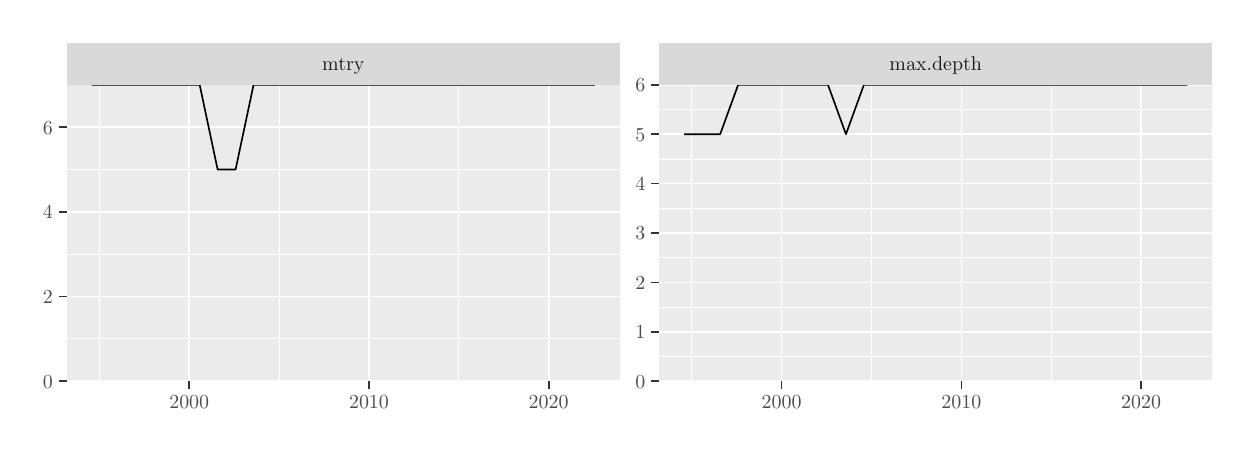
\begin{tikzpicture}[x=1pt,y=1pt]
\definecolor{fillColor}{RGB}{255,255,255}
\path[use as bounding box,fill=fillColor,fill opacity=0.00] (0,0) rectangle (433.62,144.54);
\begin{scope}
\path[clip] (  0.00,  0.00) rectangle (433.62,144.54);
\definecolor{drawColor}{RGB}{255,255,255}
\definecolor{fillColor}{RGB}{255,255,255}

\path[draw=drawColor,line width= 0.6pt,line join=round,line cap=round,fill=fillColor] (  0.00,  0.00) rectangle (433.62,144.54);
\end{scope}
\begin{scope}
\path[clip] ( 14.05, 16.81) rectangle (214.06,123.88);
\definecolor{fillColor}{gray}{0.92}

\path[fill=fillColor] ( 14.05, 16.81) rectangle (214.06,123.88);
\definecolor{drawColor}{RGB}{255,255,255}

\path[draw=drawColor,line width= 0.3pt,line join=round] ( 14.05, 32.10) --
	(214.06, 32.10);

\path[draw=drawColor,line width= 0.3pt,line join=round] ( 14.05, 62.70) --
	(214.06, 62.70);

\path[draw=drawColor,line width= 0.3pt,line join=round] ( 14.05, 93.29) --
	(214.06, 93.29);

\path[draw=drawColor,line width= 0.3pt,line join=round] ( 14.05,123.88) --
	(214.06,123.88);

\path[draw=drawColor,line width= 0.3pt,line join=round] ( 25.91, 16.81) --
	( 25.91,123.88);

\path[draw=drawColor,line width= 0.3pt,line join=round] ( 90.85, 16.81) --
	( 90.85,123.88);

\path[draw=drawColor,line width= 0.3pt,line join=round] (155.79, 16.81) --
	(155.79,123.88);

\path[draw=drawColor,line width= 0.6pt,line join=round] ( 14.05, 16.81) --
	(214.06, 16.81);

\path[draw=drawColor,line width= 0.6pt,line join=round] ( 14.05, 47.40) --
	(214.06, 47.40);

\path[draw=drawColor,line width= 0.6pt,line join=round] ( 14.05, 77.99) --
	(214.06, 77.99);

\path[draw=drawColor,line width= 0.6pt,line join=round] ( 14.05,108.59) --
	(214.06,108.59);

\path[draw=drawColor,line width= 0.6pt,line join=round] ( 58.38, 16.81) --
	( 58.38,123.88);

\path[draw=drawColor,line width= 0.6pt,line join=round] (123.33, 16.81) --
	(123.33,123.88);

\path[draw=drawColor,line width= 0.6pt,line join=round] (188.26, 16.81) --
	(188.26,123.88);
\definecolor{drawColor}{RGB}{0,0,0}

\path[draw=drawColor,line width= 0.6pt,line join=round] ( 23.14,123.88) --
	( 29.67,123.88) --
	( 36.17,123.88) --
	( 42.66,123.88) --
	( 49.15,123.88) --
	( 55.62,123.88) --
	( 62.15,123.88) --
	( 68.64, 93.29) --
	( 75.13, 93.29) --
	( 81.62,123.88) --
	( 88.11,123.88) --
	( 94.58,123.88) --
	(101.10,123.88) --
	(107.59,123.88) --
	(114.10,123.88) --
	(120.59,123.88) --
	(127.06,123.88) --
	(133.53,123.88) --
	(140.07,123.88) --
	(146.56,123.88) --
	(153.05,123.88) --
	(159.54,123.88) --
	(166.01,123.88) --
	(172.54,123.88) --
	(179.03,123.88) --
	(185.52,123.88) --
	(192.03,123.88) --
	(198.50,123.88) --
	(204.97,123.88);
\end{scope}
\begin{scope}
\path[clip] (228.11, 16.81) rectangle (428.12,123.88);
\definecolor{fillColor}{gray}{0.92}

\path[fill=fillColor] (228.11, 16.81) rectangle (428.12,123.88);
\definecolor{drawColor}{RGB}{255,255,255}

\path[draw=drawColor,line width= 0.3pt,line join=round] (228.11, 25.73) --
	(428.12, 25.73);

\path[draw=drawColor,line width= 0.3pt,line join=round] (228.11, 43.58) --
	(428.12, 43.58);

\path[draw=drawColor,line width= 0.3pt,line join=round] (228.11, 61.42) --
	(428.12, 61.42);

\path[draw=drawColor,line width= 0.3pt,line join=round] (228.11, 79.27) --
	(428.12, 79.27);

\path[draw=drawColor,line width= 0.3pt,line join=round] (228.11, 97.11) --
	(428.12, 97.11);

\path[draw=drawColor,line width= 0.3pt,line join=round] (228.11,114.96) --
	(428.12,114.96);

\path[draw=drawColor,line width= 0.3pt,line join=round] (239.97, 16.81) --
	(239.97,123.88);

\path[draw=drawColor,line width= 0.3pt,line join=round] (304.91, 16.81) --
	(304.91,123.88);

\path[draw=drawColor,line width= 0.3pt,line join=round] (369.85, 16.81) --
	(369.85,123.88);

\path[draw=drawColor,line width= 0.6pt,line join=round] (228.11, 16.81) --
	(428.12, 16.81);

\path[draw=drawColor,line width= 0.6pt,line join=round] (228.11, 34.65) --
	(428.12, 34.65);

\path[draw=drawColor,line width= 0.6pt,line join=round] (228.11, 52.50) --
	(428.12, 52.50);

\path[draw=drawColor,line width= 0.6pt,line join=round] (228.11, 70.34) --
	(428.12, 70.34);

\path[draw=drawColor,line width= 0.6pt,line join=round] (228.11, 88.19) --
	(428.12, 88.19);

\path[draw=drawColor,line width= 0.6pt,line join=round] (228.11,106.04) --
	(428.12,106.04);

\path[draw=drawColor,line width= 0.6pt,line join=round] (228.11,123.88) --
	(428.12,123.88);

\path[draw=drawColor,line width= 0.6pt,line join=round] (272.44, 16.81) --
	(272.44,123.88);

\path[draw=drawColor,line width= 0.6pt,line join=round] (337.39, 16.81) --
	(337.39,123.88);

\path[draw=drawColor,line width= 0.6pt,line join=round] (402.32, 16.81) --
	(402.32,123.88);
\definecolor{drawColor}{RGB}{0,0,0}

\path[draw=drawColor,line width= 0.6pt,line join=round] (237.20,106.04) --
	(243.73,106.04) --
	(250.23,106.04) --
	(256.72,123.88) --
	(263.21,123.88) --
	(269.68,123.88) --
	(276.21,123.88) --
	(282.70,123.88) --
	(289.19,123.88) --
	(295.68,106.04) --
	(302.17,123.88) --
	(308.64,123.88) --
	(315.16,123.88) --
	(321.65,123.88) --
	(328.16,123.88) --
	(334.65,123.88) --
	(341.12,123.88) --
	(347.59,123.88) --
	(354.13,123.88) --
	(360.62,123.88) --
	(367.11,123.88) --
	(373.60,123.88) --
	(380.07,123.88) --
	(386.60,123.88) --
	(393.09,123.88) --
	(399.58,123.88) --
	(406.09,123.88) --
	(412.56,123.88) --
	(419.03,123.88);
\end{scope}
\begin{scope}
\path[clip] ( 14.05,123.88) rectangle (214.06,139.04);
\definecolor{fillColor}{gray}{0.85}

\path[fill=fillColor] ( 14.05,123.88) rectangle (214.06,139.04);
\definecolor{drawColor}{gray}{0.10}

\node[text=drawColor,anchor=base,inner sep=0pt, outer sep=0pt, scale=  0.72] at (114.05,128.98) {mtry};
\end{scope}
\begin{scope}
\path[clip] (228.11,123.88) rectangle (428.12,139.04);
\definecolor{fillColor}{gray}{0.85}

\path[fill=fillColor] (228.11,123.88) rectangle (428.12,139.04);
\definecolor{drawColor}{gray}{0.10}

\node[text=drawColor,anchor=base,inner sep=0pt, outer sep=0pt, scale=  0.72] at (328.11,128.98) {max.depth};
\end{scope}
\begin{scope}
\path[clip] (  0.00,  0.00) rectangle (433.62,144.54);
\definecolor{drawColor}{gray}{0.20}

\path[draw=drawColor,line width= 0.6pt,line join=round] ( 58.38, 14.06) --
	( 58.38, 16.81);

\path[draw=drawColor,line width= 0.6pt,line join=round] (123.33, 14.06) --
	(123.33, 16.81);

\path[draw=drawColor,line width= 0.6pt,line join=round] (188.26, 14.06) --
	(188.26, 16.81);
\end{scope}
\begin{scope}
\path[clip] (  0.00,  0.00) rectangle (433.62,144.54);
\definecolor{drawColor}{gray}{0.30}

\node[text=drawColor,anchor=base,inner sep=0pt, outer sep=0pt, scale=  0.72] at ( 58.38,  6.90) {2000};

\node[text=drawColor,anchor=base,inner sep=0pt, outer sep=0pt, scale=  0.72] at (123.33,  6.90) {2010};

\node[text=drawColor,anchor=base,inner sep=0pt, outer sep=0pt, scale=  0.72] at (188.26,  6.90) {2020};
\end{scope}
\begin{scope}
\path[clip] (  0.00,  0.00) rectangle (433.62,144.54);
\definecolor{drawColor}{gray}{0.20}

\path[draw=drawColor,line width= 0.6pt,line join=round] (272.44, 14.06) --
	(272.44, 16.81);

\path[draw=drawColor,line width= 0.6pt,line join=round] (337.39, 14.06) --
	(337.39, 16.81);

\path[draw=drawColor,line width= 0.6pt,line join=round] (402.32, 14.06) --
	(402.32, 16.81);
\end{scope}
\begin{scope}
\path[clip] (  0.00,  0.00) rectangle (433.62,144.54);
\definecolor{drawColor}{gray}{0.30}

\node[text=drawColor,anchor=base,inner sep=0pt, outer sep=0pt, scale=  0.72] at (272.44,  6.90) {2000};

\node[text=drawColor,anchor=base,inner sep=0pt, outer sep=0pt, scale=  0.72] at (337.39,  6.90) {2010};

\node[text=drawColor,anchor=base,inner sep=0pt, outer sep=0pt, scale=  0.72] at (402.32,  6.90) {2020};
\end{scope}
\begin{scope}
\path[clip] (  0.00,  0.00) rectangle (433.62,144.54);
\definecolor{drawColor}{gray}{0.30}

\node[text=drawColor,anchor=base east,inner sep=0pt, outer sep=0pt, scale=  0.72] at (223.16, 14.33) {0};

\node[text=drawColor,anchor=base east,inner sep=0pt, outer sep=0pt, scale=  0.72] at (223.16, 32.17) {1};

\node[text=drawColor,anchor=base east,inner sep=0pt, outer sep=0pt, scale=  0.72] at (223.16, 50.02) {2};

\node[text=drawColor,anchor=base east,inner sep=0pt, outer sep=0pt, scale=  0.72] at (223.16, 67.87) {3};

\node[text=drawColor,anchor=base east,inner sep=0pt, outer sep=0pt, scale=  0.72] at (223.16, 85.71) {4};

\node[text=drawColor,anchor=base east,inner sep=0pt, outer sep=0pt, scale=  0.72] at (223.16,103.56) {5};

\node[text=drawColor,anchor=base east,inner sep=0pt, outer sep=0pt, scale=  0.72] at (223.16,121.40) {6};
\end{scope}
\begin{scope}
\path[clip] (  0.00,  0.00) rectangle (433.62,144.54);
\definecolor{drawColor}{gray}{0.20}

\path[draw=drawColor,line width= 0.6pt,line join=round] (225.36, 16.81) --
	(228.11, 16.81);

\path[draw=drawColor,line width= 0.6pt,line join=round] (225.36, 34.65) --
	(228.11, 34.65);

\path[draw=drawColor,line width= 0.6pt,line join=round] (225.36, 52.50) --
	(228.11, 52.50);

\path[draw=drawColor,line width= 0.6pt,line join=round] (225.36, 70.34) --
	(228.11, 70.34);

\path[draw=drawColor,line width= 0.6pt,line join=round] (225.36, 88.19) --
	(228.11, 88.19);

\path[draw=drawColor,line width= 0.6pt,line join=round] (225.36,106.04) --
	(228.11,106.04);

\path[draw=drawColor,line width= 0.6pt,line join=round] (225.36,123.88) --
	(228.11,123.88);
\end{scope}
\begin{scope}
\path[clip] (  0.00,  0.00) rectangle (433.62,144.54);
\definecolor{drawColor}{gray}{0.30}

\node[text=drawColor,anchor=base east,inner sep=0pt, outer sep=0pt, scale=  0.72] at (  9.10, 14.33) {0};

\node[text=drawColor,anchor=base east,inner sep=0pt, outer sep=0pt, scale=  0.72] at (  9.10, 44.92) {2};

\node[text=drawColor,anchor=base east,inner sep=0pt, outer sep=0pt, scale=  0.72] at (  9.10, 75.51) {4};

\node[text=drawColor,anchor=base east,inner sep=0pt, outer sep=0pt, scale=  0.72] at (  9.10,106.11) {6};
\end{scope}
\begin{scope}
\path[clip] (  0.00,  0.00) rectangle (433.62,144.54);
\definecolor{drawColor}{gray}{0.20}

\path[draw=drawColor,line width= 0.6pt,line join=round] ( 11.30, 16.81) --
	( 14.05, 16.81);

\path[draw=drawColor,line width= 0.6pt,line join=round] ( 11.30, 47.40) --
	( 14.05, 47.40);

\path[draw=drawColor,line width= 0.6pt,line join=round] ( 11.30, 77.99) --
	( 14.05, 77.99);

\path[draw=drawColor,line width= 0.6pt,line join=round] ( 11.30,108.59) --
	( 14.05,108.59);
\end{scope}
\end{tikzpicture}

\label{plot:RFHyperParams}
\end{figure}

\clearpage

\bibliographystyle{TUM2}
\bibliography{References}

\end{document}